\documentclass[10pt,a4paper,twoside]{book}
\usepackage[utf8]{inputenc}
\usepackage[T1]{fontenc}
\usepackage{graphicx}
\usepackage{lmodern} % Police un peu plus jolie
\usepackage{eurosym}
\usepackage{chemist}
\usepackage{enumitem}
\usepackage{moredefs}\usepackage[mla]{lips}
\usepackage{makeidx}
% à passer en dernier
\usepackage[french]{babel, varioref}
\usepackage{hyperref}

\setcounter{tocdepth}{3}
\setcounter{secnumdepth}{5}

\author{Agnès \nom{Lebatteux}}
\title{Copropriété}
\date{2010}

\hypersetup{%
	pdfinfo={%
		Title={\@title}%
		%, Subject={}%
		%, Author={Samuel \nom{Déom}}%
		, Keywords={Copropriété, Master}%
	}%
	, colorlinks = true% colore, plutot qu'encadre, les liens hypertexte
	, linkcolor = black% colore les liens internes en noir
	, urlcolor = black% colore les liens externes en noir
	, breaklinks = true% autorise les liens à être étendus sur plusieurs lignes
}

\newcommand*{\siecle}[1]{\textsc{#1}\ieme{}~siècle}
\newcommand*{\nom}[1]{\textsc{#1}}
\newcommand*{\pourcent}[1]{\nombre{#1}~\%}
\newcommand*{\montant}[1]{\nombre{#1}~\euro}
\newcommand*{\metreCarre}{m\up{2}}
\newcommand*{\surface}[1]{\nombre{#1}~\metreCarre}
\newcommand*{\prixSurface}[1]{\montant{#1}/\metreCarre} 
\newcommand*{\dioxydeDeCarbone}{\chemform{CO_2}}
\newcommand*{\I}{\textsc{i}}
\newcommand*{\II}{\textsc{ii}}
\newcommand*{\III}{\textsc{iii}}
\newcommand*{\IV}{\textsc{iv}}
\newcommand*{\V}{\textsc{v}}
\newcommand*{\VI}{\textsc{vi}}
\newcommand*{\CCH}{Code de la construction et de l'habitation}
\newcommand*{\article}[2]{article~\articleCodifie{#1}{#2}}
\newcommand*{\articleCodifie}[2]{#1.~#2}
\newcommand*{\VEFA}{\textsc{vefa}}

\newcommand*{\lrar}{lettre recommandée avec accusé de réception}

\newcommand*{\etc}{\emph{etc.}}

\newenvironment*{exemple}{\itshape}{}

\makeindex

\begin{document}
	\maketitle
	
	\frontmatter
	
	\part*{Préambule}
	
		« Un propriétaire, un bien ne sont jamais isolés ; toute
		propriété se heurte à d’autres propriétés, à d’autres libertés
		qui la limitent inévitablement" (C. Atias).
	
		\chapter*{Introduction}

\section*{Propos Liminaires}
	Le droit de la copropriété relève du droit des contrats.
	
	Le Code civil régit en effet les conventions conclues entre particuliers, en renvoyant essentiellement à la volonté des parties telle qu'exprimée dans leur accord. Il veille à la liberté et à la validité de l’échange des consentements, à la régularité de cet accord au regard de l’ordre public et pose la règle supérieure de la bonne foi des parties.
	
	Mais les temps modernes ont eu tendance à spécialiser le droit --- certains auteurs\footnote{Professeur Périnet Marquet Rapport au Congrès des Notaires de Deauville –-- mai 2003} parlent même de « balkanisation » du droit du contrat --- et peu à peu ce sont des pans entiers du contrat qui échappent au droit commun du Code civil pour faire l'objet de règles spécifiques de plus en plus complexes.
	
	En sorte que l'on peut penser que ces droits spéciaux sont en réalité des droits réglementaires et non plus des droits contractuels.
	
	L'extrême spécialisation de la réglementation présente un grand avantage : à quoi bon apprendre les principes généraux du droit dès lors qu'il suffira de connaître par coeur une réglementation dont le caractère impératif s'applique dans presque toutes les hypothèses rencontrées ?
	
	Le spécialiste sort sans aucun doute vainqueur de la confrontation entre la règle traditionnelle et la réglementation excessive : il ne suffit plus d'être juriste pour connaître la question ; il faut avant tout naviguer à l'aise dans cette réglementation.
	
	Mais la réglementation a toujours ses limites : elle ne peut tout prévoir et vient le moment où dans le silence de la loi et du décret nous devrons nous référer à la règle de droit traditionnelle.
	
	Le présent ouvrage s'adresse en priorité à des professionnels qui bien souvent connaissent –-- ou en tout cas appliquent --- tout ou partie de la réglementation ; il a pour but d'apporter à ces professionnels, comme à ceux qui découvrent la matière, non seulement une vue globale de la réglementation et l'acquisition de réflexes techniques, mais encore une connaissance des règles générales du droit et plus particulièrement de celles du Code civil en matière de contrats.
	
	En effet, une fois atteintes les limites de la réglementation, le Code civil demeure la référence supérieure dont la maîtrise permet d'atteindre véritablement le stade de la Spécialisation.

\section*{Lexique}

	\paragraph*{Copropriété}
	La copropriété est l'organisation d'un immeuble ou groupe d'immeubles dont la propriété est répartie en lots comportant chacun une partie privative et une quote part de partie commune. Cette forme existe dès l'instant qu'un immeuble est divisé entre 2 propriétaires et plus.
	
	\paragraph*{Lots}
	Chaque lot comprend une fraction d'immeuble appartenant au copropriétaire en pleine propriété (appartement, magasin, boutique, garage), dite « partie privative » et une quote-part des parties communes.
	Exemple : lot \no 1 : un appartement situé au rez-de-chaussée, à droite dans le hall d'entrée, comprenant, entrée, salon, salle à manger, chambre, cuisine, WC, salle de bains et les 75/1.000èmes des parties communes.
	
	\paragraph*{Parties privatives}
	Sont privatives les parties des bâtiments et des terrains réservées à l'usage exclusif d'un copropriétaire déterminé. Les parties privatives sont la propriété exclusive de chaque copropriétaire.
	Exemple : Les parquets et carrelages, les cloisons intérieures, les enduits des murs et plafonds, les peintures et tapisseries, les équipements et aménagements intérieurs (appareils sanitaires et de cuisine, placards).
	
	\paragraph*{Parties communes (ou choses communes)}
	Parties de l'immeuble qui sont en état d'indivision forcée entre tous les copropriétaires ou certains d'entre eux. Elles sont à l’usage ou à l’utilité de tous.
	Exemple : sols, cours, jardins, gros oeuvre des bâtiments, hall d'entrée, escaliers, toiture, etc...
	
	\paragraph*{Tantièmes}
	Les droits indivis de chaque copropriétaire sur les parties communes sont représentés par des tantièmes de propriété qui s'expriment en << \nombre{1 000}\ieme{} >>, << \nombre{10 000}\ieme{} >>, etc. Ces tantièmes sont calculés pour chaque lot en fonction de sa valeur relative, c’est-à-dire de sa consistance, de sa superficie et de sa situation sans qu'il soit tenu compte de son utilisation (article 5 de la loi qui n'est pas d'ordre public).
	Les tantièmes de propriété attribués à chaque lot déterminent le nombre de voix attribué à chaque copropriétaire ainsi que la quote part de charge commune générales.
	
	\paragraph*{Charges communes générales}
	Frais entraînés par la conservation, l'entretien et l'administration des parties communes.
	Ces frais ou charges sont en général répartis entre tous les copropriétaires au prorata de leurs tantièmes de copropriété et en tout cas, obligatoirement, en fonction de la consistance, de la superficie et de la situation de chaque lot (sans qu'il soit tenu compte de son utilisation) : Tantièmes de charges.
	
	\paragraph*{Charges relatives au services et éléments d’équipements}
	Frais entraînés par les services collectifs et les éléments d'équipement communs.
	Ces frais sont obligatoirement répartis entre les copropriétaires en fonction de l'utilité que les services et éléments présentent pour chaque lot.
	
	\paragraph*{Règlement de copropriété (autrefois dénommé « cahier des charges »)}
	Document obligatoire établi en principe au moment de la mise en copropriété de l'immeuble, et même avant :
	\begin{itemize}
		\item déterminant les droits et obligations des copropriétaires
		\item  fixant la répartition des charges,
		\item  définissant les modalités de fonctionnement du Syndicat.
	\end{itemize}
	
	\paragraph*{État descriptif de division}
	Document rendu obligatoire en matière de copropriété par le décret \no 59-89 du 7 janvier 1959, destiné à la publicité foncière, ayant pour objet l'identification de l'immeuble, sa division en lots numérotés, la description des lots avec l'indication de leurs tantièmes de copropriété. La désignation des lots est obligatoirement résumée dans un tableau récapitulatif.
	
	Exemple : lot 1 : appartement au rez-de-chaussée à gauche comprenant quatre pièces principales, une cuisine, une salle de bains.... et les 100/1.000èmes des parties communes générales.
	
	\paragraph*{Syndicat des copropriétaires}
	Collectivité qui regroupe tous les copropriétaires d’un immeuble l'ensemble des copropriétaires sans exception. Elle est dotée de la personnalité morale, ses organes de gestion sont l’Assemblée Générale, le Syndic et le Conseil Syndical.
	Le Syndicat des Copropriétaires est chargé de l'administration et de la conservation des parties communes.
	
	\paragraph*{Assemblées générales}
	Ce sont les réunions qui se tiennent au moins une fois par an, auxquelles assistent tous les copropriétaires et au cours desquelles, ils votent sur les questions intéressant l'immeuble, avec des voix proprotionnelles aux tantièmes de leur lot.
	
	Il n'y a pas d'assemblée générale extraordinaire, ni d'assemblée générale ordinaire, mais des assemblées générales aux cours desquelles certaines décisions devront être prises à la majorité simple, d'autres à la majorité absolue et même à la double majorité.
	
	\paragraph*{Syndic} 
	C'est le mandataire du syndicat des copropriétaires, élu en assemblée générale, pour administrer l'immeuble et veiller à sa conservation, ainsi qu’au respect du règlement de copropriété et des décisions d’assemblée générale. Il peut être bénévole ou professionnel.
	
	\paragraph*{Conseil syndical}
	C'est un groupe de copropriétaires élus par l'assemblée générale pour assister et contrôler le syndic.
	
	\paragraph*{Les majorités}
	Les décisions du Syndicat des Copropriétaires sont prises par les copropriétaires ayant des droits dans les parties communes concernées au cours de l’assemblée générale.
	Ces décisions sont votées nominativement en tenant compte du nombre de voix dont chaque copropriétaire dispose (ce nombre est fonction des tantièmes de propriété du lot) :
	\begin{description}
		\item[Majorité de l’article 24 de la loi (dite majorité relative)] Majorité des voix exprimées des présents ou représentés.
		\item[Majorité de l’article 25 de la loi (dite majorité absolue)] Majorité des voix des tous les copropriétaires de la loi.
		\item[Majorité de l’article 25-1 de la loi] Lorsque l'assemblée générale des copropriétaires n'a pas décidé à la majorité prévue à l'article précédent mais que le projet a recueilli au moins le tiers des voix de tous les copropriétaires composant le syndicat, la même assemblée peut décider à la majorité prévue à l'article 24 en procédant immédiatement à un second vote.
		\item[Majorité de l’article 26 de la loi (dite double majorité)] Majorité des 2/3 des voix de tous les copropriétaires représentant la majorité en nombre des copropriétaires. Cette majorité a été modifiée par l’Ordonnance du 30 octobre 2019
		\item[Majorité de l’article 26-1 de la loi] Lorsque l’assemblée générale n’a pas décidé à la majorité prévue au premier alinéa de l’article 26 mais que le projet a au moins recueilli l’approbation de la moitié des membres du syndicat des copropriétaires présents, représentés ou ayant voté par correspondance, représentant au moins le tiers des voix de tous les copropriétaires, la même assemblée se prononce à la majorité des voix de tous les copropriétaires en procédant immédiatement à un second vote.
		
		Exemple : si dans une copropriété existe 12 copropriétaires et que l’ensemble des lots représente 1.000/1.000èmes, la double majorité de l’article 26 est obtenue lorsque la résolution recueille le vote favorable de 7 (6 + 1) copropriétaires réunissant eux-mêmes 667 voix sur 1.000 (2/3 des voix).
	\end{description}

	Certaines décisions nécessitent l’unanimité des voix … donc des copropriétaires également.
	
\section*{Bibliographie}

\section*{Les acteurs en copropriété}

	\subsection*{La commission relative a la copropriété (CRC)}
	Par arrêté du 4 août 1987 le Garde des Sceaux a créé une commission relative à la copropriété, qui comprenait le représentant du directeur des affaires civiles et du sceau et celui du ministère de l'équipement, des transports et du logement, un Professeur de Droit, un Notaire et un Avocat, ainsi qu’à parité, des représentants d’association de propriétaires et d’associations représentant les administrateurs de bien.
	
	Depuis le 11 février 1994, M. CAPOULADE (Pierre), conseiller Honoraire à la Cour de cassation, était le président de la commission relative à la copropriété. M. PERINET MARQUET représentait la faculté.
	
	La Commission a rédigé des \textbf{Recommandations} sur toutes les questions relatives au statut de la copropriété et émis des \textbf{Avis} (non publiés) sur les questions qui lui étaient soumises par le Garde des Sceaux.
	
	Ces Recommandations n’ont pas valeur « normative », mais on ne connaît qu’un seul cas en jurisprudence où une Cour d’appel a refusé de faire application d’une Recommandation de la Commission.\footnote{CA Paris 1\iere Ch, 7 mai 2003, Administrer \no 359 octobre 2003, sur renvoi de cassation à propos de l’élection par vote bloqué du conseil syndical alors que le nombre de candidats était égal au nombre de postes à pourvoir.}
	
	A l’occasion de la loi ALUR, la commission a été supprimée au profit du CNTGI (dont les missions n’étaient pas cependant identiques\dots).
	
	\subsection*{Le CNTGI}
	Le CNTGI, Conseil National de la Transaction et de la Gestion Immobilières a été créé par la loi ALUR (article 24) du 24 mars 2014. Sa composition et son fonctionnement ont été modifiés par la loi du 27 janvier 2017 dite Egalité et Citoyenneté. Ces textes sont devenus caducs avec l’adoption de la loi ELAN dont l’article 53 d’origine (devenu l’article 151 de la Petite Loi) réforme profondément l’Institution.
	
	Le CNTGI doit être consulté « pour avis », notamment « sur les projets de textes législatifs ou réglementaires relatifs à la copropriété » et plus seulement sur les projets de loi relatifs à l’exercice des activités des professionnels de l’immobilier qui sont soumis à la loi Hoguet.
	
	La loi ELAN a retiré partiellement au CNTGI la fonction disciplinaire qui lui avait été donnée par la loi ALUR pour ne lui laisser, au moyen d’une Commission de contrôle des activités de transaction et de gestion immobilière, qu’un rôle d’instruction des « cas de pratiques abusives portées à la connaissance du conseil ».d’alerte auprès de la DGCCRF.
	
	Le financement de ce Conseil devait à l’origine être assuré par \textbf{le versement d’une cotisation professionnelle} par les personnes soumises à la réglementation Hoguet dont le montant aurait été fixé tous les trois ans par le Garde des Sceaux. Cette obligation de financement, très mal vécue par les professionnels, a été supprimée par la loi ELAN.
	
	\subsection*{Syndicats professionnels et associations}
	Au sein du CNTGI, quelle que soit la formule retenue par la loi ELAN, se trouvent un certain nombre de représentants des professionnels et des « consommateurs ».
	
	Les professionnels de la gestion en copropriété sont essentiellement groupés en deux syndicats professionnels qui ont pour but d’assurer la représentativité et l’influence de leur organisation professionnelle auprès des pouvoirs publics et de défendre leurs adhérents :
	\begin{enumerate}
		\item la FNAIM, numériquement le syndicat le plus important en nombre de membres (12.000 membres revendiqués) et qui consacre une grande partie de son activité aux agents immobiliers et transactionnaires ;
		\item l’Union des syndicats de l'immobilier (UNIS), regroupant également les agents immobiliers et gestionnaires mais dont l’activité principale est consacrée à la mise en valeur de la profession de syndic de copropriété et gestionnaire d’immeuble.
	\end{enumerate}
	
	Les associations dite de « consommateurs » sont essentiellement :
	\begin{enumerate}
		\item l’Association des Responsables de copropriété (ARC) qui adhère à l’UNARC (Union Nationale) et revendique l’adhésion de \nombre{14 000} syndicats de copropriétaires ; \footnote{Cette association met essentiellement en valeur la gestion des copropriétés par des syndics bénévoles (copropriétaires assurant la fonction de syndic) auxquels elle propose d’apporter ses compétences techniques, juridiques et comptables. Elle se veut un contre-pouvoir aux syndics professionnels.}
		\item l’Association Consommation, Logement et Cadre de Vie (CLCV) qui défend essentiellement les copropriétaires eux-mêmes et qui est très impliquée dans la protection de l’environnement ;
		\item  l’Union Nationale des propriétaires immobiliers (UNPI) forte de \nombre{250 000} adhérents ;
		\item  l’Association nationale de la copropriété et des copropriétaires (ANCC) historiquement dédiée aux syndicats coopératifs, mais dont la compétence a été élargie ;
		\item  la Fédération des syndicats coopératifs de copropriété (FSCC)
	\end{enumerate}

	
	\mainmatter
	
	\part{Le statut de la copropriété}
	
		\chapter{Historique de la copropriété}

	
		\chapter{Les immeubles régis par la copropriété}

\section*{Introduction}
	
	\subsection{Quel est le parc de logements en copropriété ?}
	
	Selon l’enquête INSEE de 2013, \pourcent{28,1} des logements du parc métropolitain sont en copropriété. Le reste
	relève du parc social (\pourcent{11,8}) ou du secteur libre en mono-propriété (\pourcent{60,1}). La quasi-totalité des
	logements en copropriété sont des appartements (\pourcent{94,3}), et près de la moitié sont des résidences
	principales occupées par leur propriétaire. Les autres sont occupés à titre de résidence principale par des
	locataires, ou sont des résidences secondaires ou encore des logements vacants. Dans l’habitat individuel,
	très peu sont en location : ils sont en quasi-totalité occupés par leur propriétaire, à titre de résidence
	principale ou secondaire.
	
	Le parc est relativement ancien : près des deux tiers des copropriétés dans le collectif ont au moins un
	appartement construit avant 1970 (contre un logement sur deux dans l’ensemble du parc collectif), dont
	la moitié ont été bâtis avant 1914.
	
	Si l’on s’en tient à la région Ile de France l’habitat se répartissait ainsi en 2007 :
	\begin{itemize}
		\item La monopropriété qui représente aujourd’hui \pourcent{26} de l’habitat (en nette diminution).
		\item La maison individuelle qui représente aujourd’hui \pourcent{28,5} de l’habitat (en progression)
		\item La copropriété qui a fortement progressé ces dix dernières années et qui représentait en 2007
	\pourcent{45,1} de l’habitat.
	\end{itemize}
	
	En sorte qu’au total il y avait en 2007 plus de \nombre{2 400 000} logements en copropriété pour la seule région Ile-
	de-France\footnote{Il semble qu’au total il existe actuellement plus de 8 millions de logements soumis au statut de la copropriété sur un total de 34	millions de logements environ, soit 1/4 environ soumis au statut de la copropriété (cf. INSEE Le parc de logements en France au 1er janvier	2014).}
	
	Le registre des copropriétés a permis d’affiner ces chiffres. Au 3ème trimestre 2019, les
	statistiques (pour les copropriétés recensées) sont les suivantes :
	\begin{figure}[h]
		\centering
		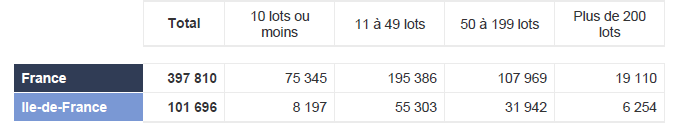
\includegraphics[width=0.7\linewidth]{images/nombreDeCoproprietesParLots}
		\caption[Nombre de copropriétés par lots]{}
		\label{fig:nombredecoproprietesparlots}
	\end{figure}
	
	\begin{figure}[h]
		\centering
		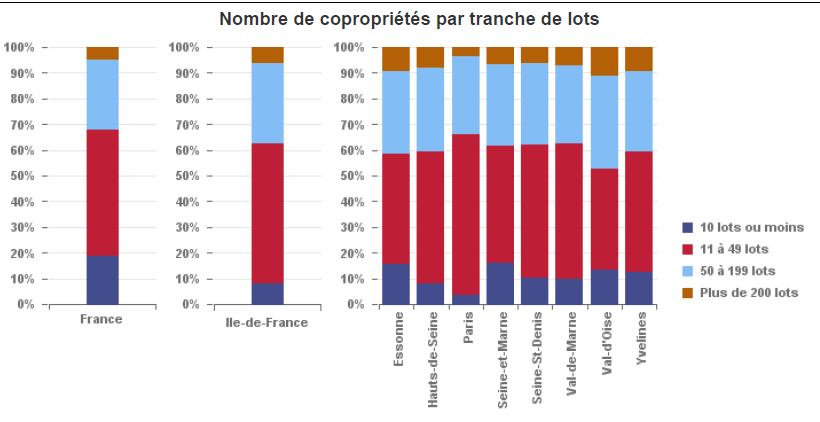
\includegraphics[width=0.7\linewidth]{images/tailleDesCoproprietes}
		\caption[Taille des copropriétés]{Taille des copropriétés (les copropriétés de moins de 10 lots sont sans doute sous représentées)}
		\label{fig:tailledescoproprietes}
	\end{figure}
	
	\subsection{Quels sont les immeubles régis par le statut de la copropriété ?}
	
		\subsubsection{Définition du champ d’application par l’article 1 de la Loi 65-557 du 10 juillet 1965 modifie par l’ordonnance du 30 octobre 2019}
		Les immeubles auxquels s’applique le statut de la copropriété sont désignés à l'article 1er de la loi du 10
		juillet 1965, ainsi rédigé après l’Ordonnance du 30 octobre 2019 :
		\begin{quote}
			« \textsc{i} - La présente loi régit tout immeuble bâti ou groupe d’immeubles bâtis à usage total ou partiel
			d’habitation dont la propriété est répartie par lots entre plusieurs personnes
			Le lot de copropriété comporte obligatoirement une partie privative et une quote-part de parties
			communes, lesquelles sont indissociables. [$\dots$]
			
			« \textsc{ii} - A défaut de convention y dérogeant expressément et mettant en place une organisation dotée de
			la personnalité morale et suffisamment structurée pour assurer la gestion de leurs éléments et services
			communs, la présente loi est également applicable :
			
			« 1\degre{} A tout immeuble ou groupe d’immeubles bâtis à destination totale autre que d’habitation dont la
			propriété est répartie par lots entre plusieurs personnes ;
			
			« 2\degre{} A tout ensemble immobilier qui, outre des terrains, des volumes, des aménagements et des services
			communs, comporte des parcelles ou des volumes, bâtis ou non, faisant l’objet de droits de propriété
			privatifs.
			
			« Pour les immeubles, groupes d’immeubles et ensembles immobiliers mentionnés aux deux alinéas cidessus
			et déjà régis par la présente loi, la convention mentionnée au premier alinéa du présent II est
			adoptée par l’assemblée générale à l’unanimité des voix de tous les copropriétaires composant le
			syndicat. »
		\end{quote}
	
		\subsubsection{Le double champs d’application du texte : Obligatoire ou supplétif}
			Avant l’Ordonnance du 30 octobre 2018, l’article 1 n’était expressément visé parmi les
			dispositions « d’ordre public » du texte.
			
			Cependant, du fait de sa rédaction, les auteurs et la jurisprudence considéraient que l'on ne
			pouvait déroger au statut de la Copropriété dès lors que la propriété de l'immeuble ou du groupe
			d'immeubles est répartie entre plusieurs personnes\footnote{
			Civ 3\degre{} 15 nov. 1989 : Bull. civ. III \no 213 p. 117; D. 1990. J. 195 note Giverdon et Capoulade
			Un immeuble avait fait l'objet d'une donation-partage et à cette occasion avait été établi un État descriptif de division créant plusieurs lots ensuite vendus à des personnes différentes. Mais cet État descriptif de division ne fixait pas de quotes-parts de parties communes attribuées à chaque lot. Un propriétaire ayant réalisé des travaux sur parties communes prétendait que la loi sur la copropriété ne s'appliquait pas du fait que s'il existait des lots, ceux-ci ne comportaient pas de quote-part de parties communes. La cour de cassation répond : << le statut des immeubles bâtis s'applique de plein droit dès que sont remplies les seules conditions prévues à l'article 1er, alinéa 1er, de la loi du 10 juillet 1965 >>.
			Également Civ. 3\degre{} Ch. 30 juin 1998, JCP G. 1998, IV, 2961	
			}, et ce alors même qu'aucun Règlement de Copropriété n'a été établi.
			
			L’ordonnance du 30 octobre 2018 consacre ce caractère d’ordre public, car l’article 1 fait
			désormais partie des textes énumérés par l’article 43 de la Loi 65-557 du 10 juillet 1965, et toute
			clause contraire est « réputée non écrite ».
			
			Toutefois, le champ d’application « obligatoire » est cantonné par le grand (\I) de l’article 1 :
			\begin{itemize}
				\item aux « immeubles ou groupes d’immeuble bâtis dont la propriété est
				repartie par lots comprenant chacun une partie privative et une quote part
				de parties communes, les deux étant indissociables » (il existe une
				indivision forcée sur les parties communes) ;
				\item\textbf{ si ces immeubles sont partiellement à usage d’habitation}, ce qui est une
				nouveauté issue de l’ordonnance
			\end{itemize}
		
			Inversement, le statut peut être écarté par une convention expresse mettant en place une
			personne morale suffisamment structurée (\II) :
			\begin{itemize}
				\item \textbf{pour un ensemble immobilier} (parcelles ou volumes distinct) dans lequel il
				n’y a pas de propriété indivise mais des terrains, volumes, équipements ou
				services « communs », c’est-à-dire d’intérêt collectif
				\item \textbf{même dans un Immeuble ou groupe d’immeuble comportant des parties
				communes en indivision}, si les lots sont tous à usage autre que d’habitation
			\end{itemize}
		
		\subsubsection{Les éléments indifférents à l’application du statut}
		
			\paragraph{L’absence d’organisation}
			
			L’absence d’assemblée générale ou de syndic (absence d’organisation de la copropriété) ne sont pas des
			conditions d’application du statut de la copropriété\footnote{Cass. Civ. 3e 14 décembre 2010 – Juris Data \no 2011-000224}. D’ailleurs, les premières immatriculations de	copropriété révèlent que \pourcent{20} des copropriétés seraient dépourvues de syndic, et ce chiffre est sans doute sous- estimé car l’immatriculation se fait alors au fil des ventes par les notaires
			
			\paragraph{L’absence d’immatriculation}
			
			De même, l’absence d’immatriculation de l’immeuble au Registre des Copropriétés est sans conséquence
			sur l’application du statut (article 1-1 de la Loi 65-557 du 10 juillet 1965 issue de la loi \no 2018-1021 du 23
			novembre 2018 dite ELAN, dernier alinéa).
			
			\paragraph{L’absence de règlement de copropriété}
			
			Lorsqu’un ensemble immobilier fait l’objet d’un état descriptif de division mais qu’il n’y a pas de règlement
			de copropriété, cet immeuble est soumis à la loi du 10 juillet 1965\footnote{Cass. Civ. 3e 1er décembre 2009 pourvoi: 08-22102}. En ce cas, l’état descriptif de division, quelle que soit sa date, approuvé ou non, revêt un caractère contractuel entre colotis (résultant de l’acte de vente) et ses clauses engagent les colotis entre eux pour toutes les stipulations qui y sont contenues\footnote{Cass. Civ. 3e 12 janvier 2011 pourvoi: 09-13822}.
			La vente de lot de copropriété en l’absence de règlement de copropriété et d’état descriptif de division
			n’est pas nulle pour indétermination de l’objet (1109 Code Civil) dès lors que les lots étaient individualisés
			et qu'il n'en résultait aucune confusion avec les lots de l'autre copropriétaire, bien que le règlement de
			copropriété soit obligatoire et doit être soumis à l’acquéreur\footnote{Cass. Civ. 3e 17 novembre 2010}.
	
	\subsection*{Plan}
		Pour déterminer le champ d’application du statut de la copropriété, il faut par conséquent distinguer :
		\begin{itemize}
			\item La copropriété des régimes voisins, dans lesquels il n’existe pas de division de
			l’immeuble entre plusieurs propriétaires ayant des droits concurrents sur les parties
			communes % (section I)
			\item La copropriété horizontale, la copropriété verticale et la construction en volume
			%(section II)
			\item Pour ce qui concerne les ensembles comprenant plusieurs bâtiments, les « groupes
			d’immeubles bâtis », pour lesquels le statut de la copropriété s’applique
			obligatoirement, des « ensembles immobiliers » pour lesquels une organisation
			différente peut être mise en place %(section III)
			\item Enfin, il sera examiné la comptabilité entre le statut de la copropriété et les
			servitudes %(section IV)
		\end{itemize}

\section{Champ d’application impératif (article \II) : immeuble ou groupe d’immeuble affecte a l’habitation}
	Depuis l’Ordonnance du 30 octobre 2019, l’article \I{} repose sur une double opposition
	\begin{itemize}
		\item l’Immeuble ou le groupe d’immeuble par opposition à « l’ensemble immobilier »
		\item et l’affectation à usage total ou partiel d’habitation par opposition à l’Immeuble ou le
		groupe d’immeuble à « destination totale autre que d’habitation »
	\end{itemize}
	
	Le champ d’application impératif du statut est désormais le suivant :
	\begin{quote}
		« \I{} - La présente loi régit tout immeuble bâti ou groupe d’immeubles bâtis à usage total ou partiel
		d’habitation dont la propriété est répartie par lots entre plusieurs personnes.
		Le lot de copropriété comporte obligatoirement une partie privative et une quote-part de parties
		communes, lesquelles sont indissociables. »
	\end{quote}
	
	\subsection{L’immeuble ou « groupe d’immeuble bâtis » caractérisé par l’homogénéité du sol}
	
		\subsubsection{Critère de distinction : homogénéité du sol}
		
			Qu'est-ce qui différencie le groupe d'immeubles bâtis où le statut sur la copropriété s'applique
			nécessairement, de l'ensemble immobilier où le statut de la copropriété ne s'applique qu'à défaut de
			conventions contraires ?
			
			Selon l’article 1, c’est l’existence de lots « comportant obligatoirement une partie privative et une
			quote-part de parties communes, lesquelles sont indissociables » qui justifie l’application
			impérative du statut, en d’autres termes la situation d’indivision forcée et perpétuelle dans
			laquelle se trouve les copropriétaires sur les parties communes qui détermine l’application du
			statut impératif.
			
			Cette situation correspond naturellement à un immeuble unique divisé en lots, mais également –-- c’est
			l’hypothèse du « groupe d’immeubles bâtis » aussi appelé « copropriété horizontale » --- à une parcelle
			cadastrale unique sur laquelle sont édifiés plusieurs bâtiments ou pavillon, tant que tous copropriétaires
			ont à la fois des « parties privatives » (appartement ou maison) et des droits indivis dans le sol (partie
			commune).
			
			Par conséquent, le groupe d’immeuble bâti relevant impérativement du statut de la copropriété se
			caractérise par l’homogénéité su sol, par opposition à l’hétérogénéité de la propriété du sol dans un
			ensemble immobilier\footnote{
			Givord, Giverdon, Capoulade, La Copropriété, Ed. Dalloz 2018 p. 85 ; Atias, Guide de la Copropriété bâtie, Edilex, 6\degre{} Edition, p. 35 ;
			Lafond Roux, Code de la Copropriété Ed. 2018 p. 11, J. Cabanac, Les ensembles immobiliers et le nouveau statut de la copropriété : Inf.
			rap. copr. mai 1966, p. 66. – Les ensembles immobiliers et la loi du 10 juillet 1965 : Gaz. Pal. 1966, 1, doctr. p. 117.– B. Leclercq, Les
			ensembles immobiliers : Rapport au 73e Congrès des notaires de France, Strasbourg 1976, p. 403 et s. – C. Lebatteux et J. Barnier-
			Sztabowvicz, Les ensembles immobiliers et l'adoption de l'organisation différente : Administrer juin 1994, p. 9 et s. – P. Capoulade :
			Copropriété et structures foncières dans la jurisprudence de la Cour de cassation : Administrer janv. 1996, p. 4 et s. – P. Capoulade et
			Cl. Giverdon, Propos sur les ensembles immobiliers : RD imm. 1997, p. 161 et s..
			} . Il y a homogénéité lorsque tous les propriétaires ont des droits réels sur
			l'ensemble du terrain servant d'assiette aux immeubles. Comme l’a écrit Pierre CAPOULADE\footnote{Administrer janvier 2001 \no 329 p. 37 et suivantes.} :
			\begin{quote}
				« Les copropriétaires possèdent des droits indivis sur l’ensemble du sol. Ils disposent sur celui-ci d’une
				quote-part numérique entrant, d’une manière indissociable avec les parties privatives, dans la composition
				du lot de copropriété ».
			\end{quote}
	
		\subsubsection{Exemples :}
			\begin{enumerate}
				\item Groupe d’immeuble bâti sur une seule parcelle comportant plusieurs Bâtiments d’habitation ou
				mixte (avec plusieurs lots), et des maisons individuelles chacune constitutive d’un lot, mais le sol
				est indivis
				\begin{center}
					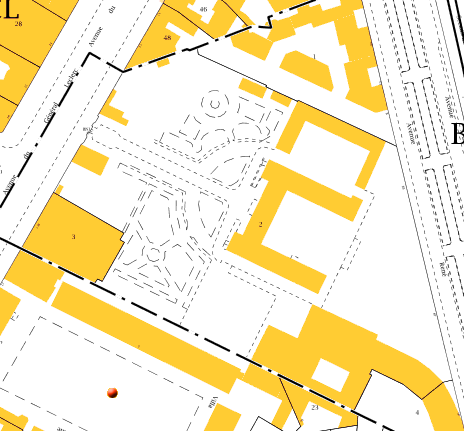
\includegraphics[width=0.7\linewidth]{images/assietteCopro}
				\end{center}
				
				\item  Plan à rez-de-chaussée d’une copropriété (en jaune pâle : parties communes :
				sol et hall), avec deux Bâtiments constitués en lot
				\begin{center}
					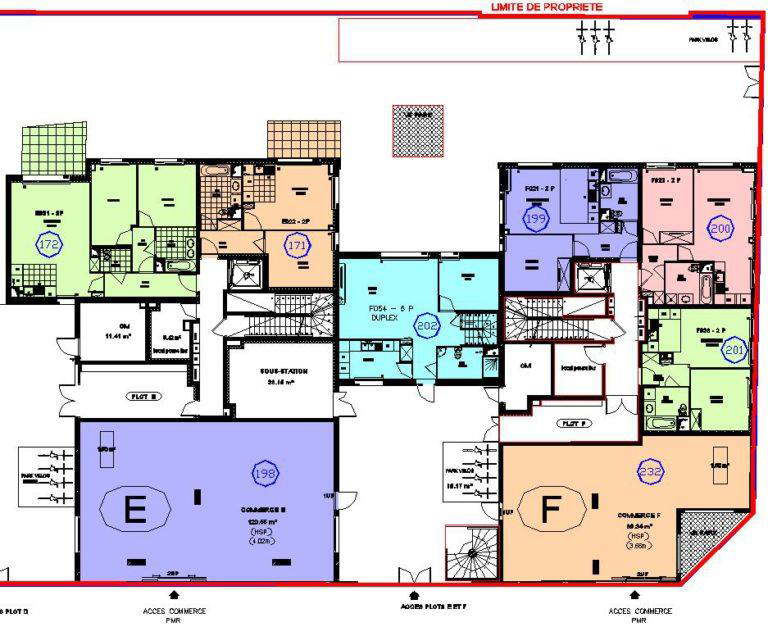
\includegraphics[width=0.7\linewidth]{images/planRdcCopro}
				\end{center}
				
				
				\item Plan de coupe d’une copropriété « verticale » classique
				\begin{center}
					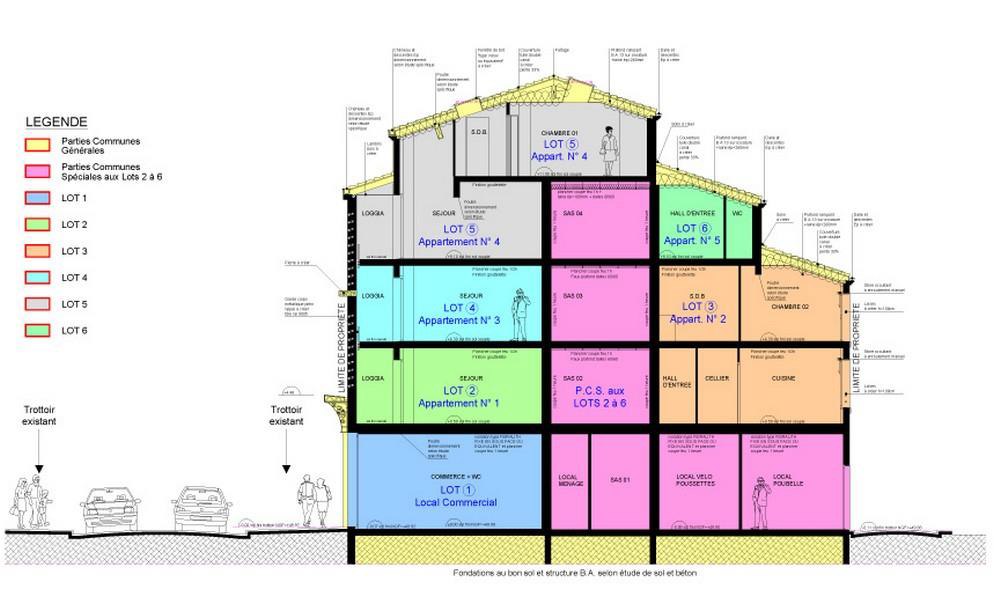
\includegraphics[width=0.7\linewidth]{images/planCoupeCopro}
				\end{center}
				
			\end{enumerate}

		\subsubsection{Conséquences}
			Lorsque la propriété du sol est homogène (appartenant indivisément à l’ensemble des copropriétaires), il
			existe un syndicat des copropriétaires de plein droit. Certes il sera possible de créer des syndicats
			secondaires pour chacun des bâtiments mais il n’y aura toujours qu’un seul syndicat « principal ».
			Ce principe a amené la Cour de Cassation à préciser qu’en cas de division d’un lot donnant vocation à la
			construction d’un bâtiment, la division de ce lot ne peut avoir pour conséquence de créer une seconde
			copropriété sur un terrain homogène\footnote{
			3\degre{} civ. 18 janv. 2018, \no 16-26072 au Bulletin et sur le site de la cour de cassation.
			} quand bien même ce lot correspondrait-il à un bâtiment séparé.
			
			La Cour d'Aix en Provence\footnote{
			16 avril 1992, Résidence l'Esplanade, Loyers et Copropriété 1993.272 et RTDI 93 p 115
			} a également retenu ce critère du régime du sol : retenant que l'immeuble
			présentait une structure homogène, l’arrêt a refusé d'assimiler l'Esplanade à un ensemble immobilier et
			a jugé en conséquence que seul le statut de la Copropriété devait recevoir application. En sorte que sur la
			demande d'un copropriétaire, les décisions de l'association syndicale libre mise en place par le promoteur
			de la Résidence lui ont été déclarées inopposables.
			
	\subsection{L’affectation a « usage total ou partiel d’habitation », nouveau critère du champ d’application impératif}

		Jusqu’à l’ordonnance du 30 octobre 2019, le statut de la copropriété s’appliquait à toutes sortes
		d’immeubles, quel que soit leur destination, dès lors que l’on se trouve en présence du régime homogène
		de la propriété du sol (chaque copropriétaire ayant des droits indivis sur la totalité du sol).
		
		En sorte que le statut s’applique bien évidemment aux immeubles d’habitation comme aux immeubles
		mixtes (habitation, professionnel, bureaux, commerces $\dots$) qui constituent la majorité en nombre
		d’immeubles soumis au statut de la copropriété. Mais le même statut s’applique également
		obligatoirement aux immeubles à usage exclusif de bureaux ou de commerces, et ce quel que soit le mode
		d’exploitation de l’immeuble dès lors que celui-ci se trouve divisé par lots.
		
		L’Ordonnance du 30 octobre 2019 revient aux origines du droit de la copropriété et aux intentions du
		législateur : que ce soit dans l’article 664 du Code civil de 1804 ou dans la loi du 28 juin 1938, les textes
		envisageaient la copropriété sous son aspect « habitation » : rappelons-nous en effet que le statut de la
		copropriété issu de la loi du 28 juin 1938 constituait le titre \II{} de cette loi, dans le titre 1\ier{} régissait les
		sociétés d’attribution qui avaient pour objet l’acquisition d’un appartement sur plan.
		
		La loi de 1965 a eu pour volonté principale d’établir un équilibre dans les droits et devoirs des
		copropriétaires à titre individuel d’une part et à titre collectif d’autre part ; implicitement cet équilibre
		concerne essentiellement les immeubles d’habitation : les travaux préparatoires de la loi de 1965 faisaient
		état de l’avenir « de l’habitat urbain ». Depuis lors s’est développée une conscience consumériste à laquelle
		l’idée du logement n’est pas étrangère. Enfin l’étude d’impact du projet de loi ELAN s’interrogeait
		justement sur la possibilité de différencier le statut selon le type d’occupation de l’immeuble.
		
		On peut s’interroger sur le point de savoir si le statut protecteur de la copropriété doit effectivement
		profiter à des immeubles exclusivement consacrés à des activités professionnelles : qu’il s’agisse de
		commerces ou d’immeubles de bureaux réalisés par des investisseurs.
		
		Le gouvernement a décidé de franchir le pas en modifiant l’alinéa 1er de la loi du 10 juillet 1965 par l’ajout
		des mots « \textit{à usage total ou partiel d’habitation} », en sorte qu’\textit{a contrario }le statut de la copropriété ne s’applique pas de plein droit aux immeubles dont la propriété est répartie par lots entre plusieurs
		personnes dès lors qu’aucun de ces lots n’a vocation à être affecté à l’habitation.
		
		Notons que pourra également échapper au statut de la copropriété un immeuble composé exclusivement
		de parkings !
		
		Cette réduction du champ d’application obligatoire du statut est tellement importante que l’Ordonnance
		a jugé utile de la réaffirmer dans l’alinéa 2 de l’article 1er de la loi en faisant état de la possibilité
		d’échapper au statut de la copropriété lorsqu’il s’agit « \textit{de tout immeuble ou groupes d’immeubles bâtis, à
		destination totale autre que l’habitation} ».
		Ainsi, le statut de la copropriété « obligatoire » est écarté, \textbf{alors même que l’immeuble est divisé par lots
		et que le sol est homogène, dès lors qu’il n’y a aucun lot à usage d’habitation}.
	
		Toutefois, l’affectation d’un sol lot à usage d’habitation (loge de gardien par exemple), aura pour
		conséquence de faire retomber l’immeuble en copropriété.

\section{Le champ d’application supplétif du statut : les ensembles immobiliers et les immeubles a destination autre que d'habitation}
	Le champ d’application du statut « par subsidiarité » (à défaut d’organisation contraire), ou supplétif est
	désormais défini, en application de l’article 1-\II{} de la Loi 65-557 du 10 juillet 1965 dans sa rédaction issue
	de l’Ordonnance du 30 octobre 2019
	\begin{quote}
		« \II. - A défaut de convention y dérogeant expressément et mettant en place une organisation dotée de
		la personnalité morale et suffisamment structurée pour assurer la gestion de leurs éléments et services
		communs, la présente loi est également applicable :
		« 1\degre{} A tout immeuble ou groupe d’immeubles bâtis à destination totale autre que d’habitation dont la
		propriété est répartie par lots entre plusieurs personnes ;
		« 2\degre{} A tout ensemble immobilier qui, outre des terrains, des volumes, des aménagements et des services
		communs, comporte des parcelles ou des volumes, bâtis ou non, faisant l’objet de droits de propriété
		privatifs.
		« Pour les immeubles, groupes d’immeubles et ensembles immobiliers mentionnés aux deux alinéas ci dessus
		et déjà régis par la présente loi, la convention mentionnée au premier alinéa du présent \II{} est
		adoptée par l’assemblée générale à l’unanimité des voix de tous les copropriétaires composant le
		syndicat. »
	\end{quote}
	
	\subsection{Les ensembles immobiliers hétérogènes}
	
		Qu'est ce qu'un ensemble immobilier ? C'est un ensemble dans lequel il existe à la fois :
		\begin{itemize}
			\item Des biens ou services « communs »: terrains, des volumes, des aménagements et des services
			communs, tels par exemple des allées et voies de desserte, un local social, des terrains de jeux
			et de sport, une piscine, des tennis, un gardiennage avec une maison de gardien, etc.
			\item Des parcelles ou volumes, bâtis ou non, faisant l’objet de droits de propriété « privatifs » ou
			« divis » (le sol de ces parcelles n’est pas en indivision forcée).
		\end{itemize}
		
		\subsubsection{L’ensemble immobilier caractérisé par « l’hétérogénéité du sol »}
			Il y a hétérogénéité lorsque l'ensemble immobilier comporte les terrains attribués à différentes personnes
			(le foncier est éclaté), aucune ne pouvant se prévaloir de droits réels (indivis) sur l'ensemble des terrains.
			Mais entre ces différentes parcelles existent des terrains communs, ou des éléments fédérateurs (indivis
			ou non)
		
			M \nom{SIZAIRE} : « à côté d'un terrain et d'éléments communs ou bien superposés à ceux-ci, il existe des propriétés ou des	copropriétés particulières : l'ensemble immobilier est juridiquement hétérogène »\footnote{
			Journées d'étude du CNEIL 22/23 nov. 1965, p. 52}
			
			M \nom{VIGNERON} : « l’ensemble immobilier tient sa spécificité du fait que les sols d’assiette font l’objet de modes d’appropriation différents, en propriété ou en copropriété selon les parcelles incluses dans cet ensemble et autonomes les unes par rapport aux autres »\footnote{
			(G. Vigneron- JurisClasseur Construction - Urbanisme > Fasc. 90-20 : STATUT DE LA COPROPRIÉTÉ. – Champ
			d'application du statut, \no 35}
			
			\paragraph{Exemples}
			
			\subparagraph{Lotissement} : toutes les parcelles font l’objet d’un droit de propriété exclusif, mais il existe des terrains, voiries, équipements d’intérêt collectifs dont la propriété est confiée à une ASL (voie = parcelle cadastrale)
			\begin{center}
				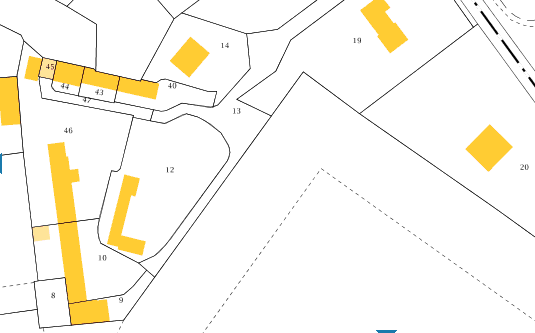
\includegraphics[width=0.7\linewidth]{images/lotissement}
			\end{center}
			
			
			\subparagraph{Voie privée} : Voie laissée en indivision avec de part et d’autres des parcelles distinctes, ou encore faisant l’objet d’une propriété de chaque riverain au droit de sa façade, jusqu’à la moitié de la voie.
			\begin{center}
				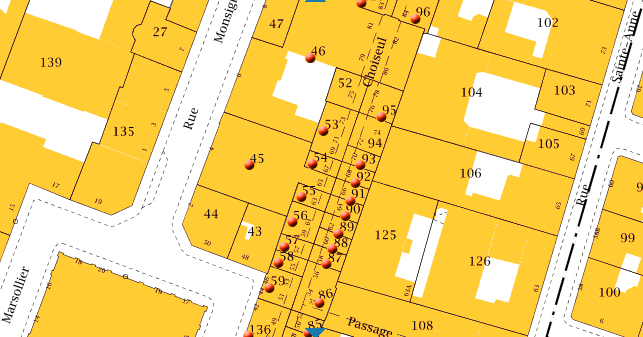
\includegraphics[width=0.7\linewidth]{images/voiePrivee}
			\end{center}
			
		
			\subparagraph{Jurisprudence antérieure à l’ordonnance}
			\begin{description}
				\item[Civ. 3ème 17 février 1999\footnote{Cour de cassation Chambre civile 3 17 Février 1999 \no 97-14.368 Bull. Association foncière urbaine libre Grand Ecran c/ associationsyndicale Italie-Vandrezanne}] : l’ensemble immobilier susceptible de faire l’objet d’une organisation différente résulte du seul fait que certains copropriétaires avaient des droits réels exclusifs sur certaines parcelles du terrain faisant ressortir l’hétérogénéité du régime juridique des fractions de l’ensemble en question.
				
				\item[Civ. 15 décembre 1993\footnote{Civ 15 décembre 1993, pourvoi: 91-12645 , au bulletin, Recueil Dalloz 1994, Somm. p. 205 (Domaine des Clausonnes)}]	: << \textit{Un lotissement comportant, selon les dispositions de l'art. R. 315-1 c. urb., division du sol en propriété ou en jouissance, privant les allotis de droits concurrents sur l'ensemble du terrain, une cour d'appel, qui constate, par motifs non critiqués, qu'un arrêté préfectoral a autorisé le lotissement et approuvé le cahier des charges et qu'une association syndicale a été constituée, d'où il résulte que l'application de la loi \no 65-557 du 10 juill. 1965 se trouve exclue, n'a pas à procéder à une recherche que ses constatations rendaient inopérante et qui n'était pas demandée} >>.
			
				\item[Paris 23\degre{} Ch 29 octobre 1997\footnote{Paris 23\degre{} Ch 29 octobre 1997 Tour Cantate Loyers et Copropriété 1998 \no 20}] Constitue un ensemble immobilier la juxtaposition d’immeubles en copropriété et d’immeubles	appartenant à une société détentrice de droits réels exclusifs sur une partie du terrain.
			\end{description}
		
		\subsubsection{L’ensemble immobilier dit « complexe » (en volumes)}
		
			\paragraph{Origine}
			
				La loi sur la copropriété ne s'applique pas nécessairement à des locaux superposés ou imbriqués, sans
				création corrélative de parties communes.
				En effet, il existe une présomption posée par l'article 552 du Code Civil, selon laquelle << la propriété du sol
				emporte la propriété du dessus et du dessous >> ; mais la preuve contraire peut être rapportée : c'est le cas
				assez fréquent d'une cave qui déborde sur le terrain voisin. Cette cave << débordante >> ne sera pas en
				copropriété avec l'immeuble dans le sol duquel elle se trouve.\footnote{
				Civ 1\degre{}, 2 avril 1962. B. \no 66, p. 54; cf également Civ 3\degre{} 11 mai 1994 RD Imm 1994, 486 pour une terrasse qui constitue
				le sol d'un immeuble et la couverture d'un autre immeuble.}
				
				La généralisation de ce mécanisme a permis la création de construction dites en « volume » (ou Ensembles
				Immobiliers Complexes) qui échappent également au statut de la copropriété.
				
				<< \emph{La volonté de limiter le gaspillage de l'espace se concrétisa avec l'apparition d'un nouveau parti
				architectural et urbanistique : << \emph{l'ensemble immobilier complexe (E.I.C.)} >>, ouvrage formant un tout,
				techniquement indivisible, où se juxtaposent, se superposent, s'imbriquent, s'articulent des volumes de
				destinations variées (habitations, activités, équipements, circulation, etc) et où l'utilisation systématique
				du tréfonds fait disparaître la notion même de sol naturel. L'objectif consiste à aménager non plus des
				terrains, mais l'espace urbain dans ses trois dimensions} >>(\nom{Walet} et \nom{Chambelland})\footnote{
				Walet et Chambelland in La Construction en Volumes (Masson Editeur, 1989)}
				
			\paragraph{Définition}
				Selon MM \nom{Walet} et \nom{Chambelland}, l'E.I.C. sera caractérisé :
				\begin{quote}
					<< 1\degre{} Par la juxtaposition et la superposition à l'intérieur \emph{d'une même structure technique},
					de volumes dont chacun \emph{abrite une fonction spécifique} et reçoit un statut \emph{approprié à
					celle-ci} ;
					<< 2\degre{} par son absence de parties communes entre ces volumes, \emph{absence due à
					l'hétérogénéité juridique de ces derniers} ;
					<< 3\degre{} par son appropriation, sa construction, sa gestion par \emph{deux ou plusieurs maîtres
					d'ouvrage} dont souvent l'un d'eux \emph{relève du droit public} ;
					<< 4\degre{} par ses contraintes de construction et de gestion entraînées à la fois par la structure
					technique et la pluralité de maîtrises de l'ouvrage et de destinations;
					<< 5\degre{} par l'intervention d'un spécialiste, promoteur ou aménageur. >>
				\end{quote}
			
				\begin{figure}[h]
					\centering
					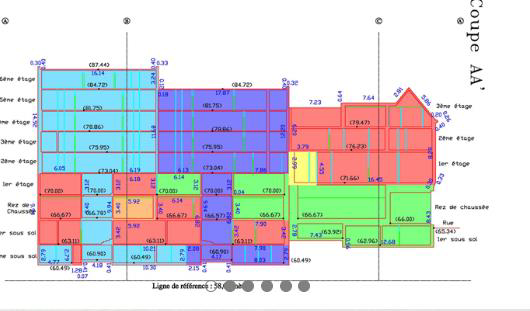
\includegraphics[width=0.7\linewidth]{images/volumetrieCoupe}
					\caption[Exemple : Urbanisme sur Dalle (Nanterre)]{}
					\label{fig:volumetriecoupe}
				\end{figure}
				)
				Le plus souvent on trouve à l’origine de cette conception :
				\begin{itemize}
					\item une dalle servant de base à l'aménagement d'une zone --- cette dalle sera un ouvrage public;
					\item  plusieurs niveaux techniques et à usage de parkings sous la dalle ;
					\item des ouvrages ou parties d'ouvrages à vocation publique également (service de mairie
					ou Tribunal de commerce par exemple à Nanterre) sur la dalle ; 
					\item  à côté de ces ouvrages à caractère public ou parfois même au-dessus on trouvera des commerces
					et des habitations.
				\end{itemize}
				
				Chaque volume sera défini en altimétrie par rapport au Nivellement Général de la France\footnote{
				Une altitude est un écart de hauteur par rapport à un niveau de référence, le niveau moyen des mers. En France, l’altitude 0 correspond au niveau moyen de la Méditerranée enregistré au marégraphe de Marseille (dans le Vieux Port) de 1885 à 1897.
				Depuis ce lieu les géomètres ont parcouru l’Hexagone pour installer des repères d’altitude par la méthode du nivellement	géométrique précis à quelques millimètres. Il y a actuellement 450.000 repères sur un réseau de \nombre{300 000} kms de long.
				}(NGF) en sorte que la propriété du volume sera comprise entre deux cotes N.G.F.
				
				A l'intérieur du volume pourront être créés plusieurs niveaux qui seront eux-mêmes soumis à un statut
				prédéterminé, par exemple le volume A sera une propriété unique (Un Commerce au niveau O) et le
				volume B une copropriété (habitations du niveau 1 au niveau 5).
				
				S'il n'existe pas de parties communes, il existe cependant une certaine imbrication entre les différents
				volumes. Ces imbrications feront l'objet de servitudes entre les volumes (servitude d'appui, d'accrochage,
				de vue, etc ...).
				
				Il n’y a pas de copropriété s’il n’y a pas de parties indivises entre les copropriétaires (parties communes)\footnote{
				Cass. Civ 3e 8 septembre 2010
				}. Ces volumes seront le plus souvent regroupés en une Association Syndicale de Propriétaires qui gérera
				l'Ensemble Immobilier.
				
			\paragraph{Volumétrie par « affectation »}
				On peut s'interroger sur la légalité d'un découpage de bâtiments qui ne correspond pas à une réalité
				physique. Mais on imagine mal les tribunaux remettre en cause un nombre aujourd'hui important
				d'opérations immobilières d'envergure\footnote{
				Sur la question Cf. Sizaire - Division en volumes et Copropriété des immeubles bâtis JCP 88.1.3367.
				}
				
				Étant toutefois observé l'abus manifeste de certains promoteurs qui pour mieux vendre certains locaux en
				les faisant échapper aux contraintes de la loi de 1965 n'hésitent pas à créer des Divisions en volumes
				purement artificiels qui comprennent deux parties : un volume commercial au rez de chaussée et un
				volume habitation pour les étages au-dessus des commerces.
				
				La loi ALUR a consacré l’organisation des immeubles en volumes… dans l’hypothèse de la scission d’une
				copropriété initiale devant donner naissance à plusieurs propriétés distinctes. L’article 28 de la loi sur la
				scission comporte désormais deux nouveaux paragraphes qui sont ainsi rédigés :
				\begin{quote}
					\textsc{iv}. – La procédure (de scission) prévue au présent article peut également être employée pour la
					division en volumes d’un ensemble immobilier complexe comportant soit plusieurs bâtiments
					distincts sur dalle, soit plusieurs entités homogènes affectées à des usages différents pour autant
					que chacune de ces entités permettent une gestion autonome. Si le représentant de l'État dans le
					département ne se prononce dans les deux mois, son avis est réputé favorable.
					
					Elle ne peut en aucun cas être employée pour la division en volumes d’un bâtiment unique. ($\dots$)
				\end{quote}
			
				Toutefois il convient d’observer qu’en excluant la division en volumes d’un bâtiment unique, le législateur
				semble considérer que la Volumétrie doit correspondre à une « autonomie de gestion ».
				
			\paragraph{Consécration par l’ordonnance du 30 octobre 2019}
				
				L’ordonnance du 30 octobre 2019 a consacré la possibilité de constituer un Ensemble Immobilier
				complexe, puisque l’article 1- \II{} vise explicitement l’hypothèse de l’ensemble immobilier composé non de
				« parcelles » mais de « volumes ».
				
				Contrairement à ce qui avait été pressenti, l’ordonnance ne restreint pas les cas dans lesquels une mise
				en Volume est envisageable, par exemple en exigeant une autonomie structurelle ou une superposition
				des domaines publics et des domaines privées. Elle se contente de renforcer les exigences concernant
				l’organisation à mettre en place pour éviter à ces ensembles de se trouver « sans gouvernail », mais ces
				exigences ne sont pas de nature à éviter certains abus ( par exemple, la prise en charge de la toiture
				exclusivement par le volume supérieur, qui se trouve être celui d’habitation).
				
				Aussi, l’ordonnance pourrait-elle avoir un effet accélérateur sur la constitution d’ensembles immobiliers
				en Volumes :
				\begin{itemize}
					\item  elle supprime le contrôle du Préfet (prévu dans la loi \no 2014-366 DU 24 MARS 2014 DITE ALUR)
					en cas de scission en Volumes
					\item  elle encourage le découpage d’un ensemble Immobilier complexe en volumes « par
					affectation », dès lors que le Volume « commerce » en pied d’immeuble, même s’il est lui-même
					divisé en plusieurs lots comportant des parties communes indivises, pourra échapper
					complètement au statut de la copropriété
				\end{itemize}
		
		\subsubsection{Les éléments fédérateurs}
			Pour être qualifié comme tel, l’ensemble immobilier doit cependant nécessairement comprendre un ou
			des éléments fédérateurs, constitués par « \emph{des terrains, des volumes, des aménagements et des services communs} » tels que, par exemple, des parcelles indivises, une impasse commune\footnote{3ème Civ., 11 février 2009, Bull. civ., III, \no 34, pourvoi 08-10109}, une chaufferie
			centrale\footnote{3ème Civ., 21 juin 2000, pourvoi \no 98-20897}, etc.
			Ces « choses communes » peuvent être en indivision forcée, attribuées de façon divise à chaque coloti (
			voie privée propriété de chaque coloti jusqu’à la moitié de la voie) ou leur propriété peut être transférée
			à l’organisme de gestion ( à l’ASL en lotissement)
			La question qui peut se poser est celle de savoir si des aménagements communs, en l’absence de terrain
			commun suffisent à constituer un ensemble immobilier : en effet l’énumération de l’article 1 – II de la loi
			issu de l’ordonnance (et avant de dernier alinéa de l’article 1) et reliée par la conjonction « et », et non ou
			Cela signifie-t’il qu’il faut « en plus » de terrains ou volumes communs, des aménagements ou des
			équipements communs ? En l’état de la jurisprudence il semble qu’il suffit d’avoir un élément commun
			pour constituer un ensemble immobilier\footnote{
			(Civ. 3\degre{} Ch. 21 juin 2000, Pourvoi \no 98-20897) – Solution critiquée par Atias ; op. cit. p. 35
			}	(par exemple une chaufferie commune).
	
	\subsection{Les ensembles immobiliers à destination autre que d’habitation (ordonnance du 30 octobre 2019)}
		Relèvent également du champ supplétif d’application de la copropropriété « tout immeuble ou groupe
		d’immeubles bâtis à destination totale autre que d’habitation dont la propriété est répartie par lots entre
		plusieurs personne »
		
		Il faut noter que les termes du \I{} et du \II{} ne sont pas totalement transposable : le \I{} (champ d’application
		obligatoire) parle des immeubles « à usage total ou partiel d’habitation », tandis que le \II{} (champ
		d’application supplétif) parle des immeubles « à destination autre que d’habitation ».
		
		Or, en principe, la destination résulte du règlement de copropriété, et elle est intangible, tandis que l’usage
		d’un lot est une question de fait, un lot pouvant librement changer d’usage (ou d’affectation), tant que ce
		changement demeure compatible avec la destination de l’immeuble.
		
		En réalité, ces deux conditions sont sans doute cumulatives. Pour qu’un immeuble puisse être soumis à un
		statut autre que la copropriété :
		\begin{itemize}
			\item il faut qu’à sa conception, donc dans le « cahier des charges » constitutif, il se trouve
				intégralement destiné à un usage autre que d’habitation ;
			\item il faut en outre que cette destination ait été respectée concrètement, car si l’immeuble devient
				à usage partiel ou total d’habitation, il retombera sous le coup du statut de la copropriété.
		\end{itemize}
	
	\subsection{L’exigence d’une organisation différente « suffisamment structurée » et « dotée de la personnalité morale » (ordonnance du 30 octobre 2019)}
		Bien que l’ordonnance ait pour l’essentiel consacré l’évolution jurisprudentielle en cours, elle crée pour
		ces immeubles soumis à un statut « alternatif » à la copropriété un cadre beaucoup plus rigide que celui
		de l’ancien article I dernier alinéa qui se contentait d’appliquer le statut aux ensembles immobiliers
		hétérogènes « à défaut de convention contraire créant une organisation différente ».
		
		Désormais, le statut redeviendra applicable « à défaut de \emph{convention y dérogeant expressément} et mettant
		en place une organisation dotée de la \emph{personnalité morale} et \emph{suffisamment structurée pour assurer}, la
		gestion de leurs éléments et services communs, la présente loi est également applicable ($\dots$) ».
		
		\subsubsection{Exigence d’une dérogation explicite}
			L’Ordonnance substitue au mot « convention contraire » les mots « convention y dérogeant
			expressément ». Ce faisant le texte reprend purement et simplement les mots qui avaient été retenus
			dans l’arrêt de la cour de cassation du 19 septembre 2012.
			
			Cette modification est heureuse : la convention à intervenir n’est pas nécessairement contraire aux
			dispositions de la loi de 1965 ; on peut concevoir en effet la mise en place d’une ASL qui outre les quelques
			dispositions impératives de l’Ordonnance du 1er juillet 2004, reprendrait pour l’essentiel les dispositions
			de la Loi 65-557 du 10 juillet 1965, par exemple quant à la répartition des charges.
		
		\subsubsection{Exigence de la création d’une personne morale}
		
			Cette précision est une codification de la jurisprudence récente de la Cour de Cassation. En effet, certaines
			voies privées, ou certains lotissements (avant 1943) sont dotés d’un cahier des charges, ou d’une
			convention d’indivision ou de servitude, indiquant les modalités de répartition des charges, voire de prise
			de décision, mais dépourvus de la personnalité morale, si bien qu’ils constituent des groupements de fait\footnote{cf. civ. 3\degre{} Ch. 31 mars 1993 \no 90-10143.}.
			
			Cette situation aboutit immanquablement à une impasse : dépourvu des attributs de la personnalité
			morale, un tel groupement ne peut ni régulariser de contrat, ni agir en justice pour préserver les
			« éléments fédérateurs », ni poursuivre judiciairement l’un de ses membres en recouvrement des charges.
			
			Aussi la cour de cassation\footnote{Civ. 3\degre{} Ch. 19 sep 2012, Pourvoi \no 11-13679 11-13789, au Bulletin} dans un arrêt du 19 septembre 2012 rendu à propos d’immeubles divisés en
			volumes, avait-elle déjà considéré que le statut ne pouvait être écarté en l’absence de personnalité
			juridique assurant l’entretien de ces éléments d’équipement:
			\begin{quote}
				« Attendu que, pour débouter la SCI [\emph{de sa demande tendant à l’application du statut de la
				copropriété}], l'arrêt [$\dots$] relève que l'état descriptif de division stipule que l'ensemble immobilier ne
				sera pas régi par la loi du 10 juillet 1965 et qu'à cette fin, l'acte identifie des volumes immobiliers de
				pleine propriété dans le cadre du régime du droit de superficie, et énonce l'ensemble des servitudes
				issues de l'imbrication de ces volumes qui permettent leur coexistence ainsi que l'attribution [de]
				\nombre{3 026}/\nombre{10 000}\iemes{} des charges générales au lot \no 4, retient que l'état descriptif de division constitue,
				relativement à ce lot, la convention contraire visée à l'article 1er, alinéa 2, de la loi du 10 juillet 1965 ;
				Qu'en statuant ainsi, sans constater la création d'une organisation différente, au sens de la loi, pour
				la gestion des éléments communs de l'ensemble immobilier, la cour d'appel a violé le texte susvisé »
			\end{quote}
		
		\subsubsection{Une personnalité morale « suffisamment structurée » -- les 3 types de	« structures » communément envisageables}
		
		On ignore pour quelles raisons l’Ordonnance a cru devoir exiger que cette personnalité morale soit
		suffisamment structurée.
		
		Si l’on prend cet exemple de l’association syndicale libre l’Ordonnance du 1er juillet 2004 édicte en son
		article 7 que « les statuts fixent son objet, son siège et ses règles de fonctionnement, précise ses modalités
		de financement et le mode de ($\dots$) recouvrement des cotisations ». Aux termes de l’article 9 de la même
		ordonnance du 1er juillet 2004 : l’association « est administrée par un syndicat composé de membres élus
		($\dots$) » et « le syndicat règle par ses délibérations les affaires de l’association ».
		
		Il est vrai cependant que les statuts peuvent être mal rédigés ou contradictoires, mais en ce cas on voit
		mal le juge requalifier l’association syndicale en syndicat de copropriété puisqu’il doit simplement
		appliquer les dispositions du droit des obligations en ce qui concerne l’interprétation des contrats : article
		1188 et suivants modifiés par l’Ordonnance \no 2016-131 du 10 février 2016.
		
		De plus, il a été jugé à maintes reprises qu'un statut d'organisation différente est exclusif du statut de la
		Copropriété : les charges seront réparties conformément aux statuts qui pourront retenir une répartition
		différente de celle organisée par la loi de 1965 (sauf dans l'hypothèse de la Société d'Attribution non
		encore dissoute) : la loi du 10 juillet 1965 est étrangère au fonctionnement d'une ASL régie par
		l’ordonnance du 1er juillet 2004 relative aux associations de propriétaires (ayant remplacé la loi du 21 juin
		1865 abrogée).
		
		Pour autant on peut cependant envisager l’hypothèse où les statuts seraient muets sur des points
		essentiels comme par exemple la majorité applicable aux décisions ou l’absence de répartition des
		cotisations entre les immeubles membres de l’association syndicale libre.
		
		En cette hypothèse et dans le premier cas (absence de mention sur les majorités applicables) le juge devra t-il faire application de la règle de l’unanimité ou pourrait-il requalifier le statut de l’ensemble immobilier
		pour le soumettre au droit de la copropriété ? Dans le second cas (absence de répartition des cotisations),
		on pourrait concevoir effectivement que le juge considère qu’il y a lieu d’appliquer le statut de la
		copropriété. En ce cas il y aurait substitution pure et simple du régime de la copropriété aux statuts de
		l’association syndicale libre.
		
		Face à cette exigence, il sera préférable, de retenir, pour administrer l’immeuble, une des formes
		communément admises pour la gestion des ensembles immobiliers.
		
		\paragraph{L'association de propriétaires de l’ordonnance du 1er juillet 2004 et le décret du 8 mai 2006}
			Ces associations de propriétaires sont en fait les anciennes associations syndicales de la loi du 21 juin 1865.
			L’association de propriétaires peut être libre ou autorisée. La forme moderne de ces Associations est
			l’Association Foncière Urbaine Libre (AFUL), prévue par le Code de l’Urbanisme pour gérer les lotissements
			(art Article L322-9-1 du Code de l’Urbanisme).
			
			La contrainte majeure concernant ces Associations Syndicales est qu’il faut recueillir le consentement
			individuel de tous les membres situés dans son périmètre. L’ASL n’est donc, le plus souvent, que constituée
			\emph{ab initio}. Sinon, l’unanimité est requise.
			
			Ces Associations Syndicales sont administrées par un « Syndicat » élu par l'Assemblée des syndicataires et
			représenté par un Président (salarié ou élu) qui est l'agent d'exécution du Syndicat. Lorsqu’elles
			comprennent des copropriétés, celles-ci peuvent être représentées à l’assemblée générale par le
			président du conseil syndical (ASL) ou le syndic (AFUL), préalablement habilité par l’assemblée générale
			de copropriété.
			
			L’Ordonnance du 1er juillet 2004 et son décret d’application imposent un contenu minimum aux statuts,
			mais ne comprennent pratiquement aucune disposition d’ordre public, ce qui laisse une grande latitude
			dans l’organisation de l’ensemble immobilier.
	
			Toutefois on peut s’inquiéter de cette trop grande liberté s’agissant notamment de la participation aux
			charges qui peut être particulièrement déséquilibrée : par exemple dans un centre commercial où
			l’opérateur pourra avoir tendance à favoriser les « locomotives » - dont les murs peuvent appartenir à une
			ou plusieurs de ses filiales - au détriment des simples « wagons » que sont les boutiques installées le long
			du mail commercial !
			
			De la même façon, les propriétaires minoritaires ne pourront en cas de décision majoritaire contraire à
			leurs intérêts invoquer l’atteinte à la destination de l’immeuble, garde-fou essentiel dans l’application du
			statut de la copropriété.
			
			Il est vrai que le même risque peut exister dans le cas d’ensembles immobiliers à vocation mixte
			(habitation, commerce, bureau). Toutefois le risque est alors limité puisqu’il ne portera que sur les
			éléments fédérateurs à plusieurs immeubles, alors que s’agissant d’un même immeuble à usage exclusif
			de bureaux et/ou de commerces, ce statut (organisation dotée de la personnalité morale et suffisamment
			structurée) s’appliquera à toutes les parties communes.
		
		\paragraph{La Société Immobilière de Gestion et d'Entretien}
		
			Souvent appelée société de location, cette société loue des immeubles ou les met à disposition de ses
			associés. Ce type de société est régi par le droit commun (article 1844 et s. du code civil).
		
		\paragraph{L'Union de syndicats de copropriétaires}
		
			C’est une organisation différente prévue à l’article 29 de la loi de 1965 et qui fait l’objet des articles 63 à
			63-4 du Décret de 1967.
			
			Par exemple, l'ensemble réalisé à la Plagne en Savoie a adopté ce schéma juridique. Notons cependant que
			pour qu'il y ait Union de Syndicats, il faut par application de la loi du 10 juillet 1965 sur la copropriété que
			cette Union comprenne au moins un syndicat de copropriété, peu importe le statut juridique des autres
			immeubles. De plus, cette structure n’est pas juridiquement stable : sauf pour les Unions issues d’une
			scission volumétrique, il ne peut être imposé à l’un des membres de l’union l’interdiction de s’en retirer.
			
			Il n’en reste pas moins que l’Union est une bonne solution pour « recouvrir » d’une personnalité juridique
			une convention de gestion qui en était jusqu’alors dépourvue, car l’adhésion de la copropriété sera votée
			à la majorité de l’article 25 (l’unanimité n’est donc pas requise).
	
	\subsection{Le passage du statut impératif au statut supplétif (et inversement)}
	
		\subsubsection{Modalité de la « sortie » du régime de la copropriété (Ord. 30 oct. 2019)}
		
			L’ordonnance prévoit les modalités selon lesquelles un immeuble déjà existant, pour lequel l’application
			du statut n’est pas ou plus obligatoire, mais qui en relèverait actuellement, pourrait se soustraire au statut
			impératif : il est exigé une décision prise à l’unanimité des copropriétaires.
		
			Bien que le dernier alinéa vise les « deux alinéas ci –dessus », donc tant l’hypothèse d’un immeuble
			pouvant échapper au statut du fait de sa destination autre que d’habitation, que celle d’un ensemble
			immobilier :
			\begin{itemize}
				\item  pour l’immeuble à destination autre que d’habitation, il est normal qu’un changement des
				règles du jeu aussi fondamental relève de l’unanimité des membres du syndicat des
				copropriétaires
				\item  toutefois, pour les ensembles immobiliers hétérogènes, soumis par « défaut » au statut de la
				copropriété, la solution peut s’avérer en contradiction avec les dispositions concernant les
				Unions de Syndicat. En effet, la constitution d’une Union devrait permettre d’échapper au
				statut de la Loi 65-557 du 10 juillet 1965, et ne requière qu’une décision à l’article 25. A moins
				que le gouvernement n’ait considéré que les Unions relevaient encore du statut ?
			\end{itemize}
			
			Par ailleurs, l’adoption de cette convention n’est pas nécessairement incompatible avec le maintien d’une
			indivision forcée sur les parties communes. Pour un immeuble de bureau, par exemple, il pourrait être
			constituée (à l’unanimité) une ASL pour l’administration des parties communes, chacun demeurant
			propriétaire de « lots » comportant une quote part indivise de parties communes. En effet, la division en
			Volumes a posteriori d’un tel immeuble serait sans doute d’une complexité inextricable.
		
		\subsubsection{Exemple de requalification : application du statut de la copropriété aux voies privées dépourvues d’organisation collective}
			
			On peut s'interroger sur la possibilité de faire appliquer la loi aux immeubles riverains d'une voie privée
			lorsque cette voie ne bénéficie pas d'un statut conventionnel (A.S.L.) ou forcé (loi sur l'assainissement de
			1912, aujourd’hui abrogée).\footnote{
			Cf D. \nom{SIZAIRE} Gazette du Palais 14 juillet 1985 p. 4 : Le statut de la copropriété des immeubles bâtis et la gestion des voies privées, cours ou jardins}
			
			Un premier arrêt de cassation, concernant le Passage de Briare\footnote{
			Civ.3ème 11 octobre 2000, \no 99-10039, Administrer janvier 2001 \no 329, comm Capoulade
			}, avait consacré ce principe, étant précisé que la propriété du sol était commune à l’ensemble des immeubles riverains. La cour d’appel avait écarté	l’application de la loi sur la copropriété puisque cette voie était bordée de propriétés distinctes. L’arrêt est cassé car « cette situation n’exclut pas de plein droit l’application du statut de la copropriété pour l’entretien, la gestion et l’administration de la voie. »
			
			La même solution a été retenue sans équivoque dans un arrêt de cassation de la 3ème Chambre de la Cour
			de Cassation du 11 février 2009\footnote{
			Cour de cassation, chambre civile 3, 11 février 2009, \no de pourvoi: 08-10109 Publié au bulletin Cassation Recueil Dalloz,
			\no 8, 26 février 2009, Actualité jurisprudentielle, p.496-497, note Yves Rouquet (“Etablissement d’enseignement et propriété
			commerciale”). Voir également la revue Loyers et copropriété, \no 4, avril 2009, commentaire \no 99, p.23-24, note Guy Vigneron
			(“Ensemble immobilier”).
			}	: la cour d’appel avait considéré que « la copropriété pure et simple
			appliquée à un ensemble immobilier n’est pas sans inconvénient et qu’il existe d’autres modes
			d’organisation différente ». La cassation se fait au visa de l’article 1er alinéa 2 (devenu l’article I-2\degre{}) de la
			loi et avec l’attendu de principe : « Attendu qu'à défaut de convention contraire créant une organisation
			différente, la présente loi est également applicable aux ensembles immobiliers qui, outre des terrains, des
			aménagements et des services communs, comportent des parcelles, bâties ou non, faisant l'objet de droits
			de propriété privatifs ».

\section{Copropriété et autres formes d’appropriation des biens}
	
	\subsection{Copropriété et monopropriété}
	
		La loi sur la copropriété ne s'applique pas lorsqu'une même personne, une même famille ou une même
		société est propriétaire de la totalité de l'immeuble (Cf. les immeubles de rapport du début du siècle).
		
		Mais dès que cette personne (pour payer le ravalement ou pour mettre l'immeuble aux normes de
		salubrité et de confort, par exemple) vend un seul appartement sur l'ensemble de ceux qui composent le
		bâtiment, le statut sur la copropriété reçoit application : par le fait de cette vente la propriété est répartie
		entre plusieurs personnes"\footnote{Civ 1ère 19 janvier 1960. Bull. \no 35 p 28}.
		
		\paragraph{Sur l’apparition de la copropriété}
		Dès lors que la propriété de l'immeuble est répartie entre plusieurs personnes, par lots comportant chacun
		une partie privative constituée d'une maison et une quote-part de parties communes, il y a lieu d'en
		déduire que le statut de la copropriété était applicable à la date où l'immeuble avait comporté deux lots
		bâtis appartenant à deux personnes différentes\footnote{Cass. Civ 3e 12 janvier 2011 Pourvoi \no 09-13822}.
		L’acte de partage qui répartit les lots de l’immeuble entre les copartageants, condition d’application du
		statut de la copropriété immobilière, marque la naissance de plein droit du syndicat de copropriété.\footnote{
		Cass. Civ. 15 mars 2011	}%(cf. Chap III)
	
		\paragraph{Sur la dissolution de la copropriété par réunion de tous les lots en une seule main}
		Il résulte de cette exigence de « division » de l’immeuble entre plusieurs propriétaires qu’une copropriété
		peut disparaître dans l'hypothèse inverse : lorsque tous les lots deviennent la propriété d'une seule
		personne (achat, héritage,...)\footnote{
		Cf. sur ce point l'article du Coneiller GUILLOT Administrer avril 1979 : La disparition du Syndicat des Copropriétaires.
		}, comme prévu désormais par l’article 46-1 de la Loi 65-557 du 10 juillet
		1965 (article 39 de l’ordonnance du 30.10.2019)% –cf infra chapitre III
	
	\subsection{La copropriété et les sociétés de construction}
	
		\subsubsection{Les sociétés d’Attributions (art 212 à 212-17 du CCH)}
			
			Les sociétés d'attribution sont les anciennes sociétés de la loi de 1938 Chapitre 1er, appelées ensuite
			Sociétés du Titre \II{} de la loi du 16 juillet 1971 (abrogée) qui relèvent des dispositions du chapitre \II{} du Titre
			1\ier{} – Statut des sociétés de construction du CCH, articles 212-1 à 212-17.
			
			Ces sociétés sont constituées par des promoteurs en vue de vendre l'immeuble, mais les capitaux
			nécessaires à la construction sont recueillis auprès des futurs propriétaires. Ces promoteurs vont
			constituer entre eux une société dont l'objet sera la construction de l'immeuble en vue de son attribution
			par fractions divises aux associés qui souscriront les parts des promoteurs (Méthode dite de Paris ayant
			succédé à la méthode dite de Grenoble).
			
			Les acquéreurs de parts ne deviennent pas propriétaires des appartements, mais associés : les parts
			acquises donnant vocation à l'attribution en jouissance de l'appartement jusqu'à dissolution de la société,
			C'est donc la dissolution ou le retrait de l'associé qui transfère à celui-ci la propriété de son appartement.
			
			C'est la Société qui est propriétaire de l'immeuble et non pas les associés, l'associé peut seulement donner ses parts en nantissement ; par contre il ne peut pas consentir d’hypothèque sur un immeuble dont il n’est pas propriétaire. Certes, la société pourrait consentir une hypothèque ; mais elle ne peut le faire au profit d’un associé sans perdre le régime fiscal de la << transparence >>. Ceci explique qu’il est plus difficile d’obtenir un crédit pour acquérir des parts de société d’attribution que pour acquérir un appartement ; d’où la liquidation de ces sociétés lorsque l’immeuble est achevé et les comptes de construction approuvés.
	
			\subsubsection*{Zoom}
			
			Le régime de ces sociétés se rapproche de celui de la copropriété : l'article L 212-2 édicte en effet que
			lorsque l'immeuble est destiné à passer en copropriété, doivent exister un règlement de copropriété et un
			état descriptif de division "avant tout commencement des travaux" ou "avant toute entrée en jouissance".
			
			Les règles de répartition des charges sont identiques aux règles posées par la loi sur la copropriété et la
			révision judiciaire de ces charges est possible dans les mêmes conditions.
			
			Cette identité n'est cependant pas complète : si le règlement de jouissance est un règlement de
			copropriété avant la lettre, la gestion de la Société même après achèvement de l'immeuble demeure régie
			par les dispositions de ses statuts et les majorités applicables sont celles des statuts, non celles prévues
			par la loi de 1965\footnote{PARIS 12 janvier 1983 R.T.D.I. 1983 p 258 et 261} : l’article L 212-1 précise au demeurant : « L’objet de ces sociétés comprend la gestion
			et l’entretien des immeubles jusqu’à la mise en place d’un statut différent ».
			Notamment, la modification de la répartition des charges entre associés doit intervenir dans les conditions
			prévues par les statuts, non en fonction de la loi du 10 juillet 1965, inapplicables au fonctionnement d’une
			société d’attribution\footnote{Civ 3\degre{} 12 fév 1997 Loyers et Copropriété mai 1997 \no 149}.
			Le passage en copropriété résultera de la première « sortie » d’un associé de la société. Il demandera
			« l’attribution des parts aux lots »), car il se formera alors une copropriété à deux : l’attributaire et la SCIA.
			Il peut aussi résulter de la dissolution de la SCIA (cf. Chapitre 3)
		
		\subsubsection{Les sociétés d’habitat participatif (art l 200-1 et s. du cch)}
	
		Il s’agit d’une création de la loi ALUR insérée dans le Livre \II{} du CCH : « TITRE PRÉLIMINAIRE : « LES
		SOCIÉTÉS D'HABITAT PARTICIPATIF » (articles L. 200-1 et suivants)
		\begin{quote}
			« L'habitat participatif est une démarche citoyenne qui permet à des personnes physiques de s'associer,
			le cas échéant avec des personnes morales, afin de participer à la définition et à la conception de leurs
			logements et des espaces destinés à un usage commun, de construire ou d'acquérir un ou plusieurs
			immeubles destinés à leur habitation et, le cas échéant, d'assurer la gestion ultérieure des immeubles
			construits ou acquis.
			« En partenariat avec les différents acteurs agissant en faveur de l'amélioration et de la réhabilitation du
			parc de logements existant public ou privé et dans le respect des politiques menées aux niveaux national
			et local, l'habitat participatif favorise la construction et la mise à disposition de logements, ainsi que la
			mise en valeur d'espaces collectifs dans une logique de partage et de solidarité entre habitants ».
		\end{quote}
		
		\paragraph{Les principales caractéristiques de ces sociétés}
		
	\begin{enumerate}[label=\arabic*)]
		\item elles ont pour vocation de construire puis de loger des associés personnes physiques dont les parts
		donneront vocation à l'attribution en propriété ou en jouissance de leur résidence principale.
		
		\item ces sociétés ont également pour objet de gérer l'immeuble une fois construit ou acquis ; cette gestion
		portant notamment sur les parties communes et les " espaces partagés" ; en d'autres termes ces sociétés
		ont également pour objet de " contribuer au développement de la vie collective" étant précisé que ces
		sociétés pourront sous certaines conditions offrir des services non seulement à leurs membres mais
		également à des tiers.
		
		\item  la responsabilité des associés est limitée à leur apport dans le capital social.
		En réalité ces sociétés auront pour " promoteurs" des personnes morales à vocation sociale (sociétés HLM,
		sociétés d'économie mixte ...) qui détiendront jusqu'à \pourcent{30} du capital social et se verront attribuer les
		logements correspondant à leur participation dans le capital social.
		
		\item Ces sociétés seront de deux types distincts :
		\begin{enumerate}[label=\roman*)]
			\item Sociétés coopératives d'habitants
			
			Les sociétés coopératives d'habitants ne donneront à leurs associés que la jouissance des logements, en
			sorte que l'immeuble restera la propriété de la société coopérative, donc l'immeuble aura un propriétaire
			unique et le statut de la copropriété ne s'appliquera pas.
			
			\item Sociétés d'autopromotion
			
			Les sociétés d'autopromotion décideront dès l'approbation de leurs statuts de choisir entre deux vocations
			distincts : soit l'attribution en jouissance des logements soit l'attribution en jouissance puis en propriété
			des logements.
			
			Si l’attribution en jouissance est prévue, l’associé pourra quand même se retirer de la société mais son
			retrait n'entraînera pas la disparition de ses parts qu'il pourra céder à un successeur choisi par lui et agréé
			par la société ou en cas de refus de ce successeur par la société, choisi par cette dernière.
		
			Si l’attribution en propriété est prévue, tout associé peut se retirer de la société une fois l’immeuble
			construit et les comptes de construction approuvés. En ce cas le retrait entraîne annulation des parts
			correspondantes et l'immeuble se trouve soumis au statut de la copropriété puisque appartenant à
			plusieurs propriétaires.
			
			Mais dans l'un et l'autre cas, l'assemblée générale statuant à la double majorité des deux tiers des voix et
			des deux tiers des associés pourra prononcer la dissolution de la société ; le partage pouvant alors
			entraîner attribution des fractions d'immeubles aux associés.
		\end{enumerate}
	\end{enumerate}
	
	\subsection{Copropriété et démembrement de propriété}
	
		\subsubsection{Location Accession de la loi du 12 juillet 1984}
			
			Même si l'article 32 de cette loi édicte que la signature d'un contrat de location est assimilée à une
			mutation, en réalité, la Copropriété ne naîtra à la vie civile que du jour où le locataire-accédant sera devenu
			réellement propriétaire au terme du contrat. La disposition de l'article 32 signifie simplement que si
			l'immeuble est soumis au régime de la Copropriété, le locataire-accédant aura pour partie les droits d'un
			copropriétaire (par exemple celui de participer et de voter sur certaines questions aux Assemblées
			Générales).
		
		\subsubsection{La copropriété et la multipropriété (Loi du 6 janvier 1986)}
	
			Le terme de multipropriété n'est pas exclusif : on rencontre en effet la propriété à temps partagé ou encore
			la propriété spatio-temporelle $\dots$ sans évoquer son appellation franglaise de \emph{société de time-sharing}.
			Le << multipropriétaire" >> est tout $\dots$ sauf copropriétaire. Il est essentiellement un acquéreur des parts ou
			actions d'une << société d'attribution d'immeubles à temps partagé >> donc sans attribution en propriété.
			C'est donc une société de type particulier.
	
			Dans ce système l'acquéreur achète les parts qui lui donneront vocation à la jouissance d'une fraction de
			l'immeuble pendant une période déterminée : huit jours à Noël ou quinze jours en été, par exemple.
			
			La loi de 1965 ne s'applique pas davantage à cette catégorie particulière de société ; cependant, compte
			tenu de l'essor de ce type d'habitat de loisir, le législateur, par une loi du 6 janvier 1986, leur a donné un
			statut spécial qui par nombre d'aspects s'inspire, en matière de gestion de l'immeuble de la société et de
			répartition des charges, du régime de la loi du 10 juillet 1965 :
			
			Par exemple le gérant de la société est nécessairement désigné (ou révoqué) par décision des associés
			représentant plus de la moitié des parts sociales (dans une Copropriété le syndic est désigné par les
			copropriétaires représentant plus de la moitié des voix de l'ensemble immobilier). De même doit exister
			un \textbf{conseil de surveillance} qui donne son avis aux dirigeants sociaux ou à l'assemblée générale sur toutes
			les questions concernant la société pour lesquelles il est consulté ou dont il se saisit lui-même.
			
			De plus les décisions votées en Assemblée Générale doivent être prises selon les cas à la majorité des parts
			sociales, à la majorité de plus de la moitié des parts sociales ou à la majorité des deux-tiers des voix des
			associés; système des trois majorités tiré du statut de la Copropriété.
			
			S'agissant de la répartition des charges, il distingue entre les charges générales (réparties
			proportionnellement au nombre de parts détenues par les associés dans le capital - article 9) et les charges
			entraînées par les services collectifs et éléments d'équipement (réparties en fonction de la situation, de
			la consistance du local et de la période de jouissance).
			
			Mais cette répartition tient compte de l'utilisation effective des lots, (les charges de ces services collectifs
			et équipements collectifs ne sont pas dues si l'associé n'occupe pas son lot) ce qui est antinomique du
			statut de la copropriété qui ne tient compte que de l'utilité des services et équipements collectifs pour le
			lot (et non de l'utilisation des lots).
		
		\subsubsection{Le BRS (Bail réel solidaire)}
		
			La loi \no 2014-366 du 24 mars 2014 dite loi ALUR a créé, à son article 164, les organismes de foncier
			solidaire (OFS). Il s’agit d’organismes sans but lucratif qui ont pour objet d’acquérir et de gérer des terrains,
			bâtis ou non, en vue de réaliser des logements et des équipements collectifs, destinés à la location ou à
			l’accession à la propriété, à usage d’habitation principale ou à usage mixte professionnel et d’habitation
			principale. Cet article a été codifié à l’article L. 329-1 du Code de l’urbanisme.
			
			L’OFS constitue ainsi un nouvel acteur foncier dont l’objet est notamment d’affecter durablement du
			foncier, bâti ou non bâti, dont ils restent propriétaires, à la construction ou à la gestion de logements en
			accession à la propriété ou en location pour des ménages sous plafond de ressources.
			Pour ce faire, le législateur a prévu un nouveau dispositif visant à dissocier les propriétés du sol et du bâti
			à travers un bail de longue durée générateur de droits réels, dont la durée est reconduite à chaque
			mutation : le bail réel solidaire (BRS).
			
			L’article L. 255-1 du Code de la construction et de l’habitation en présente les caractéristiques essentielles.
			La mise sous bail réel solidaire est une faculté réservée aux OFS. Le bail réel solidaire, d’une durée comprise
			entre dix-huit et quatre-vingt-dix-neuf ans, permet de consentir des droits réels immobiliers portant sur
			des logements en vue soit de la location, soit de l’accession à la propriété de logements. Le bail réel
			solidaire peut avoir pour objet la construction ou la réhabilitation de logements. Il peut également
			concerner une construction existante, ne nécessitant pas de travaux. Le preneur doit verser une redevance
			au bailleur en vue de la location ou de l’accession à la propriété de logements à prix modéré.
			
			La principale innovation du bail réel solidaire repose sur son caractère rechargeable. En cela, à chaque
			cession des droits réels afférents au logement par le preneur, le cessionnaire conclut un nouveau bail réel
			avec l’OFS et voit la durée de ce nouveau bail de plein droit prorogée lorsqu’un agrément est délivré
			(article L. 255-12 du Code de la construction et de l’habitation). Ainsi, tout nouveau preneur bénéficie de
			droits réels immobiliers pour une durée égale à celle prévue dans le contrat initial.
			Le BRS peut être compatible avec le statut de la copropriété :
			- le « droit au bail » est un droit réel qui peut servir d’assiette à une copropriété (comme un bail
			emphytéotique) –art L. 255-7 du Code de la construction et de l’habitation
			- on pourrait même envisager que le BRS porte sur un ou plusieurs lots de copropriété
		
		\subsubsection{L’Usufruit Locatif Social (USL -- issu de la loi \no 2006-872 du 13 juillet 2006 portant engagement national pour le logement)}
		
			Inversement, une copropriété peut être consituée uniquement, pendant un certain temps, de la nuepropriété
			des lots, tandis que l’usufruit de tous les lots est réuni en une seule main
			C’est le principe de l’Usufruit Locatif Social qui repose repose sur le principe du démembrement
			temporaire de propriété sur une période de 15 à 20 ans. Le copropriétaire acquiert la nue-propriété d’un
			bien à un prix décoté, tandis que son usufruit est cédé à un bailleur institutionnel. La pleine propriété se
			reconstitue sans formalités ni frais au terme du contrat. L’investisseur peut dès lors vendre, louer ou
			occuper son bien.
			
			Le nu-propriétaire quant à lui ne perçoit aucun loyer mais il bénéficie d’un régime fiscal favorable et le
			bailleur social lui garantit la libération du bien et sa remise en état à l’échéance de la convention.
			De règles dérogatoires au régime permettent l’administration du bien pendant la phase de
			démembrement, car la copropriété est pratiquement « suspendue » pour la gestion courante. Cependant,
			les droits du nu propriétaire sont préservés pour les décisions qui engagent l’avenir (travaux..)

	\subsection{Le bornage au sein d’une copropriete}
	
		Les propriétaires de différents lots ne peuvent intenter d’action en bornage de la partie privative de leurs
		lots au sein de la copropriété « car la propriété de l’entier immeuble demeure commune »\footnote{
		Cour d'Appel Nancy, 7 janvier 2016, \no 15/00252 – JurisData \no 2016-000162, Loyers et Copropriété 2016 \no 107
		}.
		C’est ce qui est dit par la Cour de Cassation\footnote{arrêt de rejet du 19 novembre 2015, \no de pourvoi: 14-25403, Publié au bulletin
		}, qui approuve la cour d’Appel d’avoir jugé que :
		« L'action en bornage ne peut pas être intenté dans une même copropriété, que se soit pour délimiter des
		parcelles affecter à la jouissance privative de deux copropriétaires distincts, ou des parcelles
		conventionnellement exclues des parties communes et attribuées privativement, ou des parties privatives
		dont la délimitation résulte du règlement de copropriété et de l'état descriptif de division ».
		\chapter[Naissance et disparition du Syndicat]{Naissance et disparition du syndicat des copropriétaires}

\section[Naissance et immatriculation]{Naissance et immatriculation du syndicat des copropriétaires}

	\subsection{Naissance de plein droit lorsque sont réunies les conditions de l’article 1\ier{} et immatriculation}

		\subsubsection{La constitution du syndicat des copropriétaires de plein droit}
		
			Le syndicat des copropriétaires est une des rares personnes morales dépourvues d’acte de naissance ou de constitution. En effet, le Syndicat des Copropriétaires existe dès lors que les conditions prévues par l’article 1\ier{} sont réunies, puisque le statut de la copropriété est d’application impérative.
			
			De ce fait, le législateur n’a pas voulu conditionner la naissance du Syndicat à une quelconque formalité --- il n’existe pas de déclaration préalable à la mise en copropriété contrairement à ce qui s’impose dans certains pays --- de peur de permettre à celui qui devrait accomplir cette formalité --- le promoteur notamment, en cas de construction de l’immeuble, de différer le plus longtemps possible cette formalité afin d’en éviter les contraintes.
			
			Dès qu’il nait à la vie civile, le syndicat des copropriétaires a la personnalité civile, ceci sans aucune forme particulière.
			
			Il suffit donc que l’immeuble soit divisé par lots appartenant à plusieurs personnes pour que le statut s’applique, ceci quand bien même il n’a pas été établi de Règlement de copropriété, d’état descriptif de division et quand bien même aucun syndic n’a été élu :
			
			Cette naissance de plein droit a bien évidemment des effets importants : par exemple la nécessité de s’adresser au syndicat des copropriétaires pour avoir réparation des parties communes ou remboursement des sommes avancées pour le compte du syndicat.\footnote{
			Civ. 3\degre{} Ch. 11 janvier 2012, \no 10-24413, au Bulletin ; D 2012, 219 note Y. Rouquet. En l’espèce l’un des deux copropriétaires avait réalisé des travaux conservatoires sur le sol commun et assigné l’autre copropriétaire pour avoir remboursement de sa quote-part : irrecevabilité de la demande qui aurait dû être engagée contre le syndicat des copropriétaires}
		
		\subsubsection{L’immatriculation obligatoire de certaines copropriétés}
		
			Le fait que les syndicats existent de plein droit dès que se trouvent remplies les conditions posées à l’article 1\ier{} de la loi a permis de constater une méconnaissance des copropriétés par les pouvoirs publics. Certes leur nombre est à peu près connu par l’enquête réalisée tous les cinq ans par l’INSEE et le Fichier des Logements par Commune (FILCOM) recoupé avec les données fiscales donne une idée approximative de ce nombre.
			
			Cette approximation n’avait pas grande importance à l’époque où les copropriétés relevaient totalement du droit privé, si ce n’est parfois la difficulté d’identifier le représentant du syndicat des copropriétaires.
			
			Mais depuis 1994 les autorités publiques sont amenées à participer au redressement des copropriétés en difficulté. Il est donc nécessaire de connaître beaucoup plus précisément non seulement le nombre de copropriétés mais également l’état de ces copropriétés. Suivant la proposition du rapport BRAYE, la loi ALUR a adopté l’obligation d’immatriculation des copropriétés sur un Registre spécifique. Ce sont les nouveaux articles L 711-1 à L 711-7 du \CCH, complété par le décret \no 2016-1167 du 26 août 2016 relatif au registre national d'immatriculation des syndicats de copropriétaires.
			
			\paragraph{Qui tient le Registre des Syndicats de Copropriété ?}
			
				Le registre des syndicats de copropriétaires est tenu par un établissement public de l'État (le Teneur du Registre). Par arrêté en date du 26 octobre 2016, l’ANAH a été désignée en cette qualité à compter du 1\ier{} novembre 2016.
			
			\paragraph{Le Registre des Copropriétés est un Registre dématérialisé}
			
				Le dépôt du dossier et les modifications qui y sont apportées sont dématérialisées ; la déclaration est donc faite par le $\dots$ « Télédéclarant ».
				
			\paragraph{Quels sont les syndicats concernés ?}
			
				Uniquement les syndicats dont les immeubles sont à usage total ou partiel d’habitation (au moins un lot à usage d’habitation).
			
			\paragraph{A qui incombe l’obligation d’immatriculation ?}
				
				La réponse est sans équivoque : Pour les immeubles à construire ou mis en copropriété, cette obligation incombe au notaire qui reçoit l’EDD et le RC\footnote{
					Immatriculation des syndicats de copropriétaires : le rôle du notaire ; Jacques Lafond, JCPN \no 38 – 23 Septembre 2016 ts
				} ; pour les immeubles déjà existants, il incombe au syndic d’effectuer cette immatriculation et de transmettre les actualisations nécessaires. A défaut il s’expose à une amende (pouvant aller jusqu’à \montant{20} par lot) assortie d’une astreinte recouvrées par le Teneur du Registre (art. L 711-6 CCH). Si un acte est reçu par un notaire sur un immeuble non immatriculé, le notaire
				procèdera à l’immatriculation et le syndic paiera l’amende ! Bien évidemment le syndic ne pourra pas se faire rembourser cette amende par le syndicat des copropriétaires. De plus le syndicat non immatriculé ou dont les données ne sont pas à jour ne pourra percevoir de subventions de l’Etat.
				
			\paragraph{Le contenu de l’immatriculation.}
			
				Les informations à porter au Registre sont fixées par Décret en Conseil d’Etat ; il s’agit du Décret \no 2016-1167 du 26 août 2016.
				
				Elles sont de deux catégories (art. L 711-1 CCH) :
				\begin{itemize}
					\item  d’une part les informations permettant d'identifier le syndicat, de préciser son mode de gestion et de connaître les caractéristiques financières et techniques de la copropriété et de son bâti, notamment le nom, l'adresse et la date de création du syndicat ainsi que, le cas échéant, le nom du syndic et le nombre et la nature des lots
					
					\item d’autre part les informations financières, les informations sur une mise sous administration judiciaire, la mise en oeuvre d’une procédure de carence ou de sauvegarde.
							
					Mais les informations « financières » seront limitées si l’immeuble comporte moins de dix lots à usage de logements, de bureaux ou de commerces, dont le budget prévisionnel moyen sur une période de trois ans consécutifs est inférieur à \montant{15 000}.
				\end{itemize}
			
			\paragraph{Les modalités de télédéclaration}
		
				La télédéclaration se fait en plusieurs temps.
				
				\subparagraph{La création d’un compte de télédéclarant.}
				Soit le télédéclarant est un « professionnel » : notaire, syndic, mandataire ad hoc, administrateur judiciaire ; auquel cas il aura un compte général auquel il « rattachera » la copropriété concernée.
				Soit le déclarant est un syndic bénévole, auquel cas il remplira directement le formulaire de sa copropriété.
				
				\subparagraph{La déclaration de la copropriété concernée.}
				Le télédéclarant fournit au Teneur de Registre tous les documents et renseignements prévus par l’arrêté du 26 octobre 2016, Annexe 1 à 7 (certaines annexes concernant les renseignements à fournir chaque année et celles à fournir en cas de changement de syndic, tant par le syndic sortant que par le nouveau syndic).
			
				\subparagraph{L’immatriculation du syndicat des copropriétaires}
				Une fois complétés les renseignements demandés, l’ANAH fournit au Télédéclarant un \no d’im\-ma\-triculation qui sera unique pour le syndicat des copropriétaires tout au long de son existence.
				
				\subparagraph{Conservation des données pendant 5 ans}
								L’article R 711-15 prévoit que les données fournies sont conservées pendant 5 ans
			
			\paragraph{La mise à jour des informations}
			
				Doivent être portées au Registre :
				\begin{itemize}
					\item toute modification dans les données du Registre ;
					\item à l’issue de chaque exercice comptable les données financières actualisées.
				\end{itemize}
			
				C’est ainsi qu’en cas de changement de syndic, le syndic sortant doit informer le Teneur de Registre de la cessation de ses fonctions et son successeur doit à son tour informer le Teneur de Registre de ce qu’il est le nouveau représentant légal du syndicat des copropriétaires.
				
				Précisons que dores et déjà il est possible d’accéder au site du Teneur de Registre et de télécharger les formulaires à compléter sur le site \url{http://www.registre-coproprietes.gouv.fr/} .
			
			\paragraph{Qui peut accéder aux informations portées au Registre ?}
			
				\begin{enumerate}
					\item \textbf{Le notaire}, qui doit porter le numéro d'immatriculation de la copropriété dans les actes de vente.
					\item \textbf{Les copropriétaires} ont un droit d'accès aux données relatives au syndicat dont ils font partie et peuvent solliciter le syndic aux fins de rectification des données erronées.
					\item \textbf{L'État} et ses services ainsi que ses opérateurs, les EPCI compétents en matière d'habitat, les départements et les régions obtiennent du teneur du registre communication des informations du répertoire relatives à chaque copropriété située sur leur territoire.
					\item \textbf{Des tiers}, selon des conditions précisées par décret en Conseil d'État pris après avis de la Commission nationale de l'informatique et des libertés (CNIL).
				\end{enumerate}
			
			\paragraph{Date d’entrée en vigueur de ces nouvelles dispositions.}
				\begin{enumerate}[label=\alph*)]
					\item Tous les immeubles à usage total ou partiel d’habitation dès à présent soumis au statut de la copropriété doivent être immatriculés avant le 31 décembre 2018.
					\item Pour les immeubles neufs ou mis en copropriété : l’immatriculation devra se faire automatiquement à compter du 1er décembre 2016.
				\end{enumerate}
		
	\subsection{Naissance a la date de la division de l’immeuble par lots}
	
		Ne sont soumis de plein droit au statut de la copropriété que tous « les immeubles bâtis dont la propriété est répartie entre plusieurs personnes $\dots$ ».
		
		Par conséquent, le Syndicat des Copropriétaires prend naissance à la plus tardive des deux dates suivantes :
		\begin{itemize}
			\item division de l’immeuble par lots comprenant chacun une quote part de parties communes et une partie privative, division qui se traduit en principe par la rédaction d’un Règlement de copropriété et d’un État descriptif de division ;
			\item existence d’un immeuble bâti, pour les immeubles vendus en VEFA.
		\end{itemize}
		
		\subsubsection{Vente par appartements d'un immeuble ancien déjà construit}
		
			L’article 1\ier{}-1 (rédaction de la loi ELAN) consacre la jurisprudence existante et édicte :
			\begin{quote}
				« En cas de mise en copropriété d’un immeuble bâti existant, l’ensemble du statut s’applique à compter du premier transfert de propriété d’un lot ».
			\end{quote}
			
			C'est le cas de l'immeuble de rapport vendu par appartements par son propriétaire.
			
			Celui-ci va procéder ou plutôt faire procéder par un ou plusieurs hommes de l'art (géomètre, expert, notaire, avocat) à l'établissement d'un Règlement de Copropriété, et d’un état descriptif de division, puis vendre un par un les lots issus de cette division.
	
			Le syndicat des copropriétaires va naître dès la première vente entre l'ancien propriétaire qui sera propriétaires de tous les lots à l'exclusion d'un seul et l'acquéreur de ce lot : en effet dès cette première vente la propriété de l'immeuble est répartie entre plusieurs personnes.
			En pratique on relève très souvent des modifications au Règlement de Copropriété et parfois des contradictions qui tiennent au fait que l'acquéreur a étudié le Règlement de Copropriété qui lui est soumis par le vendeur avant la signature de l'acte authentique de vente et tente d'obtenir divers avantages que le vendeur, désireux d'en finir pour réaliser la vente, accepte de prendre en compte.
		
		\subsubsection{Dissolution de la Société d'Attribution ou retrait d'associé (Sociétés du Titre \II{} de la loi du 16 juillet 1971)}
		
			Ces sociétés constituées pour la construction ou l'acquisition d'un immeuble en vue de sa division par fractions destinées à être attribuées aux associés en propriété ont donc pour vocation d'être dissoutes pour laisser place au régime de la Copropriété.
			
			L'immeuble construit, les associés réunis en Assemblée Générale Extraordinaire approuvent les comptes de construction et décident de la liquidation de la Société. Ils désignent un liquidateur qui aura notamment pour mission d'établir un projet de partage que signeront (ou pourront contester) individuellement les associés. Les Associés se réuniront pour approuver les comptes de liquidation. Il ne restera plus alors qu'à signer l'Acte de Partage. Par cette signature de l'acte de partage chaque associé se voit attribuer la propriété du lot dont il n'avait jusque lors que la jouissance.
			
			Toutefois les associés peuvent préférer rester en société nonobstant l'achèvement de l'immeuble et l'approbation des comptes de construction. Dans cette hypothèse cependant tout associé peut demander à se retirer de la Société et à se voir attribuer la propriété de son appartement : il exerce la faculté de retrait anticipé. Le retrait est simplement constaté par acte authentique signé par le retrayant et le représentant légal de la société.
			
			L'associé ne peut demander son retrait que s'il remplit trois conditions :
			\begin{itemize}
				\item être à jour de tous les appels de fonds nécessaires à la réalisation de l'objet social (la jurisprudence ne prend en considération que les appels de fonds nécessaires à la construction de l’immeuble et non les appels de fonds relatifs à la gestion de l’immeuble une fois construit).
				\item justifier que l'achèvement de l'immeuble social et sa conformité avec l’État descriptif de division ont été constatés par l'Assemblée Générale des Associés.
				\item justifier que l'Assemblée Générale des Associés a décidé des comptes définitifs de l'opération.
			\end{itemize}
			
			Toutefois l'associé peut demander au Tribunal de Grande Instance de faire ces constatations et mettre en œuvre la procédure de retrait malgré le refus ou la passivité des organes de direction de la Société.
			
			Dans les deux cas évoqués (dissolution ou retrait anticipé), la loi sur la copropriété s'appliquera à compter de la signature de l'acte authentique :
			\begin{itemize}
				\item en cas de liquidation il n'existe plus que des copropriétaires.
				\item en cas de retrait la copropriété fait coexister la société et le retrayant ; c'est alors une Copropriété à deux personnes.
			\end{itemize}
		
			Relevons toutefois un intéressant arrêt de la Cour d'Appel de Versailles du 27 juin 1991\footnote{Rev. Dr. Imm 1991, 3\degre{} T, p. 337} qui a affirmé que la Copropriété naissait le jour de l'Assemblée ayant approuvé les comptes de liquidation. C'est en effet cette Assemblée qui procède à l'attribution des lots conformément aux statuts et à l’État descriptif de division. Mais cette décision demeure isolée. L’opinion généralement admise étant que la copropriété naît au moment de l’attribution à chaque associé de sa part divise\footnote{Cf. Givors, Giverdon, Capoulade, La Copropriété Dalloz Ed 2018 \no 111.31}.
		
		\subsubsection{Partage en nature de l'immeuble ou licitation des lots}
		
			Lorsqu'un immeuble échoit à plusieurs héritiers, ceux-ci se trouvent placés sous le régime de l'indivision régie par les articles 812 et suivants du Code Civil. Tant que l'immeuble demeure en indivision, il appartient à une même famille et n'est donc pas soumis au statut de la Copropriété : il n’y a pas attribution des parts aux lots, et chacun est propriétaire d’une quote part virtuelle de l’immeuble.
			
			Cependant, << Nul n'est tenu de rester dans l'indivision >> en sorte que tout indivisaire est en droit de demander à sortir de l'indivision et à se faire attribuer, après partage de l'immeuble, la quote-part d'immeuble à laquelle il a droit.
			
			Préalablement au partage de l'immeuble les héritiers feront établir par le notaire un Règlement de Copropriété et un état descriptif de division.
			
			Si les héritiers ou co-indivisaires sont d'accord sur l'attribution des lots l'immeuble sera partagé en nature. En cas de désaccord des héritiers, les lots seront vendus sur licitation, les héritiers pouvant bien entendu se porter acquéreurs de lots.\footnote{Toulouse 18 Jan. 88 - juris Data \no 043735}
			
			Par contre, dès la première attribution (signature de l'acte de partage ou licitation) l'immeuble entre dans le champ d'application de la loi du 10 juillet 1965.

			Relevons que le nouvel article 1\ier{}-1 de la loi n’envisage comme point de départ du statut de la copropriété dans un immeuble existant que l’hypothèse du premier transfert de propriété du lot, alors qu’il eut été plus exhaustif d’ajouter « ou de la première attribution d’un lot ».
		
		\subsubsection{Vente d’un lot de S.C.I. d’attribution sur poursuites judiciaires.}
		
			Hypothèse plus originale où la Copropriété est imposée par voie de justice : la vente sur poursuites judiciaires d'une partie du patrimoine d'une Société d'Attribution. On peut envisager effectivement le cas où un créancier d'une société d'attribution ayant inscrit une hypothèque conventionnelle ou judiciaire sur l'immeuble propriété de la Société poursuit la vente judiciaire d'une partie de l'immeuble seulement (la valeur de cette partie d'immeuble étant suffisante pour l'indemniser de sa créance). Dans cette hypothèse l'adjudicataire sera copropriétaire de l'immeuble avec la Société saisie.
		
		\subsubsection{Surélévation d'un immeuble appartenant à un propriétaire}
		
			Dans cette hypothèse, le propriétaire d'un immeuble construit va céder à un tiers le droit de surélever son immeuble en y construisant un ou plusieurs étages supplémentaires. Une convention de copropriété devra être établie avec rédaction d'un Règlement de Copropriété et d'un État descriptif de division.
			
			Le statut de la copropriété s’appliquera dès la cession du lot « droit de surélever ».
		
		\subsubsection{Location vente ou location attribution}
		
			Si la location-vente est fréquente appliquée à un lot d'un immeuble déjà soumis au droit de la Copropriété, il arrive également que l'immeuble soit réalisé par une société qui soumettra l'ensemble au régime de la location-vente. Hypothèse qui se rencontre essentiellement dans le domaine de la Coopérative H.L.M.
			
			La société d'H.L.M. demeurera propriétaire jusqu'à ce que soit réalisée la promesse de vente. Mais dès l'origine un état descriptif de division et un Règlement de Copropriété auront été établis. Rappelons que la location accession est régie par les dispositions de la loi du 17 juillet 1984 qui emporte différentes conséquences sur le statut de la Copropriété, par exemple participation du locataire acquéreur aux Assemblées Générales de copropriété et même au Conseil Syndical.
			
	\subsection{Naissance a la date de l’achèvement de l’immeuble}
	
		\subsubsection{L’article 1\ier{}-1 de la loi du 10 juillet 1965}
	
			Pour la réalisation d’un immeuble à construire, les promoteurs peuvent constituer entre eux une société, de vente d'immeuble (art. L 210-1 et s. CCH pour les sociétés civile) , dont l'objet est l'acquisition et la
			vente d'appartements. Les fonds nécessaires à la construction étant réunis, partie en fonds propres des promoteurs et partie grâce aux prêts promoteurs consentis par les banques.
			
			Le candidat acquéreur n'est pas associé à la Société de construction mais achète directement son local qui lui sera livré soit achevé soit en l'état futur d'achèvement,
			
			Si l'immeuble est vendu << achevé >>, la Copropriété prend naissance dès la première vente.
			
			Si l'immeuble est vendu en l'état futur d'achèvement la Copropriété prend naissance dès achèvement de l'immeuble.
			C’est ce qui est expressément mentionné dans l’article 1\ier{}–1 nouveau de la loi du 10 juillet 1965 qui est ainsi rédigé :
			« Pour les immeubles à construire, le fonctionnement de la copropriété découlant de la personnalité morale du syndicat de copropriétaires prend effet lors de la livraison du premier lot ».
			Ce faisant le législateur de 2018 n’a fait que consacrer légalement une jurisprudence relativement constante\footnote{Civ 3\degre{} 20 déc 1976, JCP 1978, II, 18800, Obs. Guillot.}, quand bien même certaines décisions de cours d’appel avaient cru devoir affirmer que le statut aurait été applicable dès la première vente en l’état futur\footnote{Paris 23\degre{} Ch. 22 sep 1995, Loyers et Copropriété 1996 \no 80 ; Versailles 22 mai 1984, Rev. Dr. imm. 1984 p. 351 ; Aix 16 avril 1992 Loyers et Copropriété 1993 \no 275.}.
	
		\subsubsection{Construction d'un bâtiment unique.}
		
			S'agissant de vente en l'état futur d'achèvement le décret d'application de la loi du 3 janvier donne une définition de cet achèvement :
			\begin{quote}
			Art 261-1 C.C.H.\\
			<< L'immeuble ($\dots$) est réputé achevé ($\dots$) lorsque sont exécutés les ouvrages et sont installés les éléments d'équipement qui sont indispensables à l'utilisation, conformément à sa destination, de l'immeuble faisant l'objet du contrat. Pour l'appréciation de cet achèvement les défauts de conformité avec les prévisions du contrat ne sont pas pris en considération lorsqu'ils n'ont pas un caractère substantiel, ni les malfaçons qui ne rendent pas les ouvrages ou éléments ci-dessus précisés impropres à leur utilisation >>.
			\end{quote}

			Cet achèvement n’est donc pas subordonné à la livraison de tous les lots, ou encore à l’obtention du certificat de conformité.
		
		\subsubsection{L’immeuble vendu en l’état futur d’inachèvement}
		
			La loi ELAN a modifié le \CCH sur la vente en l’état futur d’achèvement, en ajoutant à l’article L 261-15 qui traite du contrat préliminaire à la VEFA un \II{} ainsi rédigé :
			\begin{quote}
				« \II{}. – Le contrat préliminaire peut prévoir qu’en cas de conclusion de la vente, l’acquéreur se réserve l’exécution de travaux de finition ou d’installation d’équipements qu’il se procure par lui-même. Le contrat comporte alors une clause en caractères très apparents stipulant que l’acquéreur accepte la charge, le coût et les responsabilités qui résultent de ces travaux, qu’il réalise après la livraison de l’immeuble. ($\dots$)
				
				Un décret en Conseil d’État précise les conditions d’application du présent \II{}, notamment la nature des travaux dont l’acquéreur peut se réserver l’exécution »
			\end{quote}
			
			Bien évidemment ce texte n’entrera en application qu’après publication du Décret.
			
			Pour autant il est ici question de travaux d’achèvement et non de parachèvement en sorte que les travaux que l’acquéreur se réserve peuvent porter sur des ouvrages ou éléments d’équipement indispensables à l’utilisation du lot (équipements de la salle de bains par exemple).
			
			Dans cette hypothèse faudra-t’il attendre que l’acquéreur ait réalisé ces travaux ou éléments d’équipement indispensables pour faire application du statut ?
			
			Pour des raisons pratiques et de texte, la réponse nous paraît devoir être négative et la date à retenir pour l’application du statut devrait être la livraison du premier lot $\dots$ même non achevé.
		
		\subsubsection{Pluralité de bâtiments}
		
			Il est très délicat en revanche de déterminer l'achèvement d'un ensemble de bâtiments livrés successivement (Problème des tranches successives de construction) et il est en conséquence difficile de déterminer la date à laquelle le statut de la Copropriété va recevoir application.
			
			Or, la loi s'applique à << tout immeuble bâti ou groupe d'immeubles bâtis >>.
			
			Ce texte est susceptible de deux interprétations :
			\begin{itemize}
				\item soit l'on considère que la loi n'est applicable qu'à l'achèvement du groupe d'immeubles --- lorsque le groupe est construit ;
				\item soit l'on considère que la loi s'applique dès achèvement du premier bâtiment --- dès qu'il y a un immeuble bâti.
			\end{itemize}
		
			Dans un arrêt du 4 décembre 1979\footnote{3\degre{} Ch Civ. B \no 218 p. 171} la Cour de Cassation a admis implicitement que la loi devait recevoir application dès achèvement du premier bâtiment.
			Alors que les autres bâtiments n'étaient pas construits, ce premier bâtiment achevé s'était constitué en syndicat secondaire. Une telle constitution d'un syndicat secondaire n'était possible que dans l'hypothèse où la loi de 1965 recevait application. C'est ce qu'a décidé la Cour de Cassation.
			
			Cette solution n'est plus guère discutée aujourd'hui : en fait elle constitue une réponse pratique à un problème difficile. La solution contraire aurait créé un << vide juridique >> : quel aurait été en effet le régime applicable au bâtiment achevé qui, par suite des retards souvent apportés à la réalisation des travaux de construction par << tranches successives >>, serait resté seul achevé pendant plusieurs mois, voire plusieurs années ?
			
			Au demeurant la rédaction du nouvel article 1\ier{}-1 qui fait application du statut dès la livraison du premier lot ne fait pas de distinction entre la VEFA passée dans le cadre d’un bâtiment unique ou dans le cas d’une pluralité de bâtiments.
		
			La jurisprudence précitée devrait continuer de s’appliquer : le statut s’applique dès la livraison du premier lot dans le premier bâtiment ; pour les bâtiments non construits, le vendeur sera considéré comme propriétaire des lots correspondant à ces bâtiments, mais ne participera qu’aux charges générales.
		
		\subsubsection{Le problème du lot transitoire}
			
			\paragraph{Historique}
			
				Étant admis que la loi reçoit application dès achèvement du premier bâtiment, doit-elle être appliquée au seul bâtiment achevé ou à l'ensemble des lots, que ceux-ci soient construits ou non ?
				
				Ce d'autant que la technique le plus souvent appliquée dans la Construction par << Tranches Successives >> est celle dite du lot transitoire\footnote{Autrement appelé selon Mr \nom{CAPOULADE} dans son étude pour le Rapport de la Cour de Cassation de 1994 : << lot d'attente >>, << lot par anticipation >> ou << lot parthénogénique >>}.
				
				\begin{quote}
					En pratique le Promoteur de l'ensemble constitue des lots intermédiaires, généralement un lot par bâtiment à construire. Par exemple si cinq bâtiments sont prévus, l’État descriptif de division comprendra cinq lots intermédiaires 100, 200, 300, 400 et 500.

					Chacun de ces lots étant défini non par l'addition d'une partie privative et de tantièmes généraux de copropriété, mais par un droit de construire un bâtiment qui comprendra un nombre de tantièmes généraux de la Copropriété, correspondant à l’ensemble des tantièmes du futur bâtiment.
				
					Lors de l'édification du premier bâtiment le lot 100 est << éclaté >> en autant de lots qu'il y aura de locaux principaux et accessoires dans ce bâtiment, de telle sorte que le lot 100 sera annulé et remplacé par exemple par les lots 101 à 152. Avec l'édification du deuxième bâtiment le lot 200 sera remplacé par les lots 201 à 260, etc.
				\end{quote}
				
				Ce lot transitoire est-il véritablement un lot de copropriété alors qu'il ne comprend pas de parties privatives ? La doctrine avait en effet douté de l'applicabilité de la loi à ce type de lot qui ne comporte pas de véritable "partie privative", ou plutôt, dont la partie privative ne présente pas de consistance matérielle.\footnote{Giverdon et Bouyeure, ADMINISTRER déc 81, p. 7.}
				
				La Cour de Cassation a finalement admis l’existence des lots transitoires, notamment par un important arrêt du 15 novembre 1989\footnote{Bulletin \no 213, p. 117; D 90. J. 216, note Giverdon et Capoulade} à propos de la saisie immobilière de lots transitoires
				\begin{quote}
					<< Retenant que chacun des lots saisis, placé par l'auteur de la division sous le régime de la copropriété, comprenait selon l'état descriptif, le droit exclusif d'utiliser une surface déterminée du sol pour y édifier des constructions conformément à un permis de construire délivré..., ainsi qu'une quote-part de la propriété du sol et des parties communes, la cour d'appel a exactement décidé... que le lot privatif du débiteur constituait un immeuble par nature pouvant faire l'objet d'une saisie immobilière >>.
				\end{quote}
				Et surtout par un arrêt SCI SALENGRO du 3 juin 1991\footnote{3\degre{} Ch. Civ. du 3 juin 1991 (JCP 92, \I{}, 3560)} aux termes duquel le lot transitoire ou intermédiaire est un véritable lot de copropriété, en sorte que dès l'achèvement du premier bâtiment le régime de la Copropriété va s'appliquer à l'ensemble immobilier, parties bâties et non bâties et que la SCI promotrice, en sa qualité de propriétaire des lots transitoires participera aux Assemblées Générales de la Copropriété.
				
				On retiendra également un arrêt du 14 novembre 1991 par lequel la cour de cassation a rejeté un pourvoi à l'encontre d'un arrêt par lequel la cour d'appel
				\begin{quote}
					« Retenant à bon droit que les lots dits << transitoires >> ne sont pas assujettis à un régime particulier, en a exactement déduit$\dots$ que la SCI était copropriétaire au sens de la loi du 10 juillet 1965 »
				\end{quote}.
	
			\paragraph{Le nouvel article 1\ier{} alinéas 2 et 3} 

				La loi ELAN a tenu compte de cette jurisprudence pour ajouter un nouvel alinéa à l’article 1er qui est ainsi rédigé :
				\begin{quote}
					« Ce lot peut être un lot transitoire. Il est alors formé d’une partie privative constituée d’un droit de construire précisément défini quant aux constructions qu’il permet de réaliser sur une surface déterminée du sol, et d’une quote-part de parties communes correspondante. (art. 59 bis D)
					
					« La création et la consistance du lot transitoire sont stipulées dans le règlement de copropriété. »
				\end{quote}
			
			\paragraph{La construction future doit être précisément définie}
	
				Ce nouvel article est très important.
				
				La jurisprudence ayant validé le lot transitoire acceptait parfaitement que celui-ci ne soit en aucune façon défini. Par exemple, un arrêt du 3 novembre 2016\footnote{Civ. 3\degre{} Ch. 16 novembe 2016, Pourvoi \no 15-14895 15-15113, Inédit} a considéré qu’était parfaitement valable le lot appartenant à une société , constitué du droit de construire sur une partie du terrain, sans aucune précision quant à la future construction alors que le demandeur au pourvoi avait fait valoir que : « le droit de construire mentionné dans la description d'un lot de copropriété ne peut en constituer la partie privative qu'à la condition d'être concrètement défini dans sa consistance et son implantation » . De façon lapidaire la cour de cassation a simplement répondu : « a cour d'appel a retenu, à bon droit, que le lot de la société constituait un lot privatif composé pour sa partie privative du droit exclusif d'utiliser le sol pour édifier une construction et d'une quote-part de parties communes et en a exactement déduit que la société était titulaire d'un lot transitoire.
				
				Jurisprudence d’autant plus favorable au titulaire du lot que le droit à construire sur le lot transitoire n'est pas soumis aux règles d'autorisation de la copropriété de l’article 25 dès lors qu'en vertu du règlement de copropriété son titulaire bénéficie du droit de construite « tous bâtiments et constructions »\footnote{Cass. Civ. 3e 8 juin 2011 ; \no de pourvoi: 10-20276 Publié au bulletin Revue des Loyers juillet 2011 page 322, note Jean-Marc \nom{Roux}}. De même il a été jugé que le promoteur, qui a édifié sur le lot transitoire un bâtiment à usage de garage et qui n'a fait qu'user d'un droit reconnu par le règlement de copropriété, n'était pas tenu de solliciter pour construire l'autorisation de l'assemblée générale dans la mesure où la nature et l’affectation étaient définies\footnote{Cass. Civ. 3e 4 novembre 2010}.
				
				Cette jurisprudence avait un effet déstabilisateur à l’intérieur de la copropriété du fait de la totale liberté dont bénéficiait le titulaire du lot transitoire.
				Le nouvel article 1er alinéa 2 réagit contre cette jurisprudence en imposant justement que le lot transitoire soit précisément défini :
				\begin{itemize}
					\item quant à sa surface au sol ;
					\item quant à la construction à réaliser ;
					\item quant aux quotes-parts attribuées à ce lot transitoire.
				\end{itemize}
				
				De plus, ce lot transitoire doit non seulement figurer comme tel dans l’état descriptif de division mais il doit également être mentionné et décrit dans le règlement de copropriété.\footnote{Nous verrons ultérieurement que l’état descriptif de division ne se confond pas avec le règlement de copropriété.}
			
			\paragraph{Dispositions transitoires prévues par la loi ELAN}
	
				En principe ces nouvelles dispositions ne devraient s’appliquer qu’aux lots transitoires créés postérieurement à la publication de la loi ELAN, en application du principe de non-rétroactivité des lois.
				
				La loi ELAN en décide autrement en imposant des dispositions transitoires ainsi rédigées :
				\begin{quote}
					– Les syndicats des copropriétaires disposent d’un délai de trois ans à compter de la promulgation de la présente loi pour mettre, le cas échéant, leur règlement de copropriété en conformité avec les dispositions relatives au lot transitoire de l’article 1er de la loi \no 65-557 du 10 juillet 1965 fixant le statut de la copropriété des immeubles bâtis.
					
					À cette fin et si nécessaire, le syndic inscrit à l’ordre du jour de chaque assemblée générale des copropriétaires organisée dans ce délai de trois ans la question de la mise en conformité du règlement de copropriété. La décision de mise en conformité du règlement de copropriété est prise à la majorité des voix exprimées des copropriétaires présents ou représentés.
				\end{quote}
				
				Ce texte posera certainement des difficultés d’application : Sera-t’il seulement applicable lorsque l’état descriptif de division comportera un lot transitoire non défini ou pourra-t’il être recevoir application dans l’hypothèse où le droit de construire figurera seulement dans le règlement de copropriété.
				
				En tout cas dès la première assemblée générale suivant la publication de la loi ELAN les syndics devront vérifier si les états descriptif de division comprennent des lots transitoires non précisément définis ni quant à la surface au sol ni quant à la construction projetée et en ce cas proposer à l’assemblée générale de modifier le règlement de copropriété pour y inscrire la définition du lot transitoire.
				
				Comment se fera cette définition ? Il semble difficile d’imposer au titulaire du lot une description du bâtiment à construire.
				
				A quelle majorité l’assemblée générale se prononcera sur cette modification du règlement de copropriété qui ne concerne ni l’administration de l’immeuble ni l’usage des parties communes , seules hypothèses de modifications du règlement de copropriété à la double majorité de l’article 26 de la loi ? Doit-on considérer que cette adaptation du règlement de copropriété relève de la majorité de l’article 24 f) de la loi ?
				Ce droit de construire sera-t’il caduc si l’assemblée générale n’a pas défini le lot transitoire dans le délai de 3 ans de la publication de la loi ?

			\paragraph{Jurisprudence complémentaire sur le lot transitoire}
			
				La jurisprudence, tirant les conséquences de l’’existence du lot provisoire, condamne les clauses du règlement de copropriété qui ne font participer aux assemblées générales et aux charges que les propriétaires des lots construits\footnote{Civ 3\degre{} 30 juin 1998 - Administrer janvier 1999 p. 62, note \nom{CAPOULADE}.} : le titulaire d’un lot transitoire doit obligatoirement être convoqué aux assemblées générales (à défaut il pourra en demander l’annulation pendant dix ans), et doit participer aux charges communes générales (assurances et frais de gestion notamment) $\dots$
				
				La modification d’un droit de construire attaché à un lot dit << transitoire >> pour l’étendre à des activités annexes et/ou complémentaires relève de la double majorité de l’article 26 de la loi du 10 juillet 1965 et non de l’unanimité\footnote{Cass. Civ. 3e 30 novembre 2010 30 novembre 2010 \no de pourvoi: 09-72386, non publié}.
	
\section{Disparition du syndicat des coproprietaires}

	Nous venons de voir précédemment dans quelles conditions un immeuble qui appartenait à une seule personne se trouve du fait de sa division entre plusieurs propriétaires soumis au statut de la copropriété.
	
	L’hypothèse inverse peut se rencontrer : un immeuble divisé en plusieurs lots appartenant à des copropriétaires différents va devenir la propriété d’une seule personne\footnote{Il ne faut pas confondre cette hypothèse avec la situation qui résulte de l’application des dispositions de l’article 28 de la loi sur la copropriété en cas de retrait d’un ou plusieurs lots de la copropriété d’origine. En effet aux termes de cette loi, la scission entraîne la disparition du syndicat des copropriétaires d’origine. Cette question sera traitée ultérieurement.}.
	
	La disparition du syndicat peut également résulter de son $\dots$ annulation par le juge !
	
	\subsection{La disparition du syndicat pour l’avenir}
	
		\subsubsection{La dissolution de plein droit du syndicat des copropriétaires, et sa survie pour les besoins de la liquidation}
		
			La réunion de tous les lots entre les mains d’un même propriétaire entraîne, de plein droit, la disparition du Syndicat\footnote{Cass. Civ. 3e 28 janvier 2009 pourvoi: 06-19650 Publié au bulletin} du fait que disparaît l’une : « la réunion de tous les lots entre les mains d'un même propriétaire avait entraîné de plein droit la disparition de la copropriété ».

			C’est pourquoi la cour de cassation\footnote{Civ 3ème Ch 4 juillet 2007, pourvoi: 06-11015 Publié au bulletin, Loyers et Copropriété 2007 \no 204} dans un arrêt du 4 juillet 2007 pose le principe selon lequel la réunion de tous les lots entraîne la disparition de la copropriété.
			
			Ce principe étant posé, reste à en découvrir les conséquences.
			
			\medskip
			
			Aux termes de l’article 1844–8 du code civil la société civile se survie pour les besoins de sa liquidation. Aucune disposition spécifique n’a été prévue dans la loi du 10 juillet 1965. Un syndicat des copropriétaires n’est pas une société ! Dès lors peut-on soutenir que le syndicat des copropriétaires se survie pour les besoins de sa liquidation ?
			
			\medskip
			
			Une réponse positive à cette question a été donnée par la cour de cassation\footnote{Civ 3ème Ch 5 déc 2007, pourvoi: 07-11188 07-11204 Publié au bulletin Loyers et Copropriété 2008 \no 43} dans un arrêt du 5 décembre 2007 dont les enseignements sont les suivants :
			\begin{itemize}
				\item la personnalité morale du syndicat subsiste pour les besoins de sa liquidation,
				\item la liquidation du syndicat des copropriétaires ne peut se faire sous le régime du droit de la copropriété - le liquidateur peut être désigné à l’unanimité des anciens propriétaires
				\item le Syndicat peut également être représenté par un mandataire ad hoc dans les procédures en cours, à la demande de tout intéressé.\footnote{Cour de cassation chambre civile 3 27 avril 2017 \no de pourvoi: 16-11278 Non publié au bulletin Jurisdata}
			\end{itemize}
			La demande était fondée sur l’article 1844-8 code civil. La cour de cassation ne vise pas cet arrêt : cela signifie-t’il qu’elle écarte effectivement les règles de liquidation des sociétés civiles ?
			
			\begin{quote}
				(la cour d’appel ayant) retenu à bon droit qu'en cas de réunion de tous les lots entre les mains d'une même personne, aucune disposition de la loi du 10 juillet 1965 n'avait vocation à régir la liquidation de la copropriété et que sa personnalité morale subsistait pour les besoins de sa liquidation, et constaté que l'assemblée générale tenue entre tous les anciens copropriétaires après la vente des lots avait désigné à l'unanimité M. Z$\dots$ aux fonctions de liquidateur amiable, la cour d'appel en a exactement déduit, abstraction faite d'un motif surabondant relatif à la représentation de chaque copropriétaire par le liquidateur, que la fin de non-recevoir soulevée par M. X$\dots$ devait être rejetée
			\end{quote}
			
		\subsubsection{Disparition d’une copropriété horizontale}
	
			Dans une copropriété horizontale les propriétaires de pavillons souhaitent mettre fin à la copropriété.
		
			Si cette demande est consécutive à la cession des VRD à la Commune, les copropriétaires décideront simplement de se partager le terrain d’assiette de la copropriété, en sorte que chaque propriétaire
			possèdera en pleine propriété son pavillon et le terrain d’assiette de la construction (et éventuellement le jardin).
			
			Il ne s’agira pas d’une scission de la copropriété, mais d’un partage pur et simple qui peut s’effectuer à la suite d’une décision unanime de tous les copropriétaires décidant de s’attribuer mutuellement le sol suivie d’un acte notarié de partage auquel comparaîtront tous les copropriétaires. Cette décision sera complétée par la désignation d’un liquidateur du syndicat des copropriétaires.
			
			S’il subsiste des VRD communs, l’assemblée générale pourra décider de les apporter en propriété à une ASL qu’elle constituera concomitamment\footnote{Cf. La revue fiscale du patrimoine \no 7-8, Juillet 2012, form. 7 par Jacques Lafond}. Mais attention lorsque les biens des copropriétaires sont grevés d’hypothèques.
	
		\subsubsection{Le statut de la copropriété ne s’applique pas à la liquidation du syndicat}
		
			Dès lors que la loi du 10 juillet 1965 ne s’applique plus à l’immeuble dont la propriété n’appartient qu’à une seule personne, on voit mal pour quelle raison le statut de la copropriété survivrait à la disparition du syndicat des copropriétaires.
			
			C’est la position qu’adopte la cour de cassation dans l’arrêt précité du 5 décembre 2007 :
			\begin{quote}
				« (la cour d’Appel) ayant retenu à bon droit à qu’en cas de réunion de tous les lots entre les mains d’une même personne, aucune disposition de la loi du 10 juillet 65 n’avait vocation à régir la liquidation de la copropriété $\dots$ »
			\end{quote}
			
			Dès lors en cas de dissolution du syndicat des copropriétaires, il appartient :
			\begin{itemize}
				\item - soit à l’assemblée générale du syndicat des copropriétaires avant la cession du dernier lot à une seule et même personne ;
				\item soit aux anciens copropriétaires agissant à l’unanimité ;
				\item soit à tout intéressé --- et principalement au propriétaire unique --- une fois la dissolution de plein droit réalisée ;		
			\end{itemize}
			de désigner ou de faire désigner par le juge statuant sur requête un liquidateur au syndicat des copropriétaires.
			
			Ce liquidateur pouvant bien évidemment être désigné avant dissolution du syndicat des copropriétaires par l’assemblée générale des copropriétaires sous condition suspensive de la réunion de tous les lots entre les mains d’une seule et même personne. Il peut être également dit par l’assemblée que le liquidateur ne prendra ses fonctions qu’au jour où l’ensemble des lots aura été réuni entre les mains d’une seule personne.

			Ce liquidateur se verra conférer les pouvoirs habituels du liquidateur d’une personne morale.
		
		\subsubsection{Les conséquences de la liquidation du Syndicat des Copropriétaires}
		
			De questions complémentaires doivent être résolues :
			\begin{itemize}
				\item qui doit être convoqué par le liquidateur pour l’approbation de ses comptes de liquidation ?
				\item les droits et actions du syndicat des copropriétaires sont-ils transmis de plein droit à l’acquéreur unique de tous les lots ?
			\end{itemize}
			Ici encore nous ne disposions d’aucune jurisprudence sur la question. Certes, l’article 28 de la loi, en cas de scission d’une copropriété, affirme bien que celle-ci emporte dissolution du syndicat d’origine.
			
			\paragraph{Qui est concerné par les opérations de liquidation ?}
			
			Le liquidateur devra convoquer en assemblée l’ensemble des personnes qui étaient copropriétaires au jour de la dissolution de la copropriété. C’est entre ces personnes qu’il fait les comptes et c’est à elles qu’il demande le complément nécessaire à l’apurement des dettes du syndicat en cours de liquidation.
			
			\paragraph{Les droits et obligations des copropriétaires sont-ils transmis à l’acquéreur unique ?}
			
				\subparagraph{Principe général}
				
				Contrairement à une opinion qui avait été émise par certains auteurs, l’acquéreur unique ne se trouve pas aux droits et obligations du syndicat des copropriétaires.
			
				Certes, il convient de citer un arrêt de la cour de cassation\footnote{Civ 3ème 12 septembre 200, Loyers et Copropriété 2007 \no 228. Bull Civ.} en date du 12 septembre 2007 qui reconnaît à l’acquéreur unique le bénéfice de l’action à l’encontre de l’assureur dommages ouvrage appartenant précédemment au syndicat des copropriétaires.
		
				Mais cet arrêt ne signifie en aucune façon que l’acquéreur se trouve au droit du syndicat des copropriétaires : il reprend purement et simplement le principe relatif à l’assurance dommages ouvrage
				qui veut que le l’action bénéficie aux propriétaires successifs de l’immeuble pendant la durée de la garantie décennale.
				
				Dans un arrêt de cassation\footnote{Civ. 3ème 2 octobre 2013, \no de pourvoi: 12-17098, non publié au Bulletin ; Loyers et Copropriété jan 2014 \no 27} du 2 octobre 2013, la Cour de Cassation, au visa de l’article 1165 du code civil et 14 de la loi de 1965, rappelle : «qu’en l'absence de clause expresse, la société bénéficiaire de l'apport, venue aux droits de la société apporteuse, n'était pas tenue de plein droit des obligations personnelles du syndicat ». La cour de cassation prend sa décision sur le fondement de l’art. 1165 du code civil aux termes duquel les convenbtions n’ont d’effet qu’entre les parties.
				
				\subparagraph{Le nouvel article 28 de la loi}
				
				Il est dérogé au principe que nous venons d’évoquer par le nouvel article 28 de la loi en matière de scission de copropriété. En effet cet article comprend désormais trois nouveaux paragraphes ainsi rédigés :
				\begin{quote}
					« La répartition des créances et des dettes est effectuée selon les principes suivants :
				
					« 1\degre{} Les créances du syndicat initial sur les copropriétaires anciens et actuels et les hypothèques du syndicat initial sur les lots des copropriétaires sont transférées de plein droit aux syndicats issus de la division auquel le lot est rattaché, en application du 3\degre{} de l’article 1251 du code civil ;
				
					« 2\degre{} Les dettes du syndicat initial sont réparties entre les syndicats issus de la division à hauteur du montant des créances du syndicat initial sur les copropriétaires transférées aux syndicats issus de la division. » ;
				\end{quote}
				
				On peut dès lors considérer que ce nouveau texte est une exception au principe général qui ne s’applique qu’à l’hypothèse de la scission d’une copropriété.
				
				Il est regrettable que nous ayons désormais deux régimes distincts de liquidation d’un syndicat des copropriétaires selon les causes de cette disparition !
				
				Ce nouveau texte légal est au demeurant surprenant puisqu’il fait « application » de l’article 1251 3\degre{} (ancien) du code civil selon lequel la subrogation a lieu « au profit de celui qui, tenu pour d’autres au paiement de la dette, avait intérêt de l’acquitter » : certes désormais le syndicat issu de la scission est bien tenu pour le syndicat d’origine en liquidation, des dettes de ce dernier, mais la transmission des créances de l’ancien syndicat sur les copropriétaires a lieu au profit du nouveau syndicat avant que ce dernier se soit acquitté des dettes de l’ancien syndicat.

	\subsection{La disparition du syndicat du fait de son annulation par le juge}
	
		Cette question concerne l’annulation d’un syndicat secondaire irrégulièrement créé.
		
		Dans une affaire PIGUET c/ Syndicat Le Consul\footnote{Civ. 3\degre{} 20 mai 2009 pourvoi: 07-22051 08-10043 08-10495 Publié au bulletin Loyers et Copropriété sep 2009 \no 218}, le Règlement de copropriété avait prévu l’existence d’un syndicat principal et de plusieurs syndicats secondaires alors que les conditions matérielles de séparation des bâtiments n’étaient pas réunies (cf. Troisième Partie – Le Syndicat secondaire).
		
		Quarante ans après l’entrée en application du Règlement de copropriété les consorts PIGUET ont demandé au juge d’annuler la clause du Règlement de copropriété prévoyant la constitution des syndicats secondaires. La Cour d’Appel annule la clause du Règlement de copropriété mais refuse de déclarer inexistants les syndicats secondaires : « Le syndicat secondaire institué par une clause réputée non écrite du Règlement de copropriété est censé n’avoir jamais existé ».
		
		La Cour d’Appel refuse de prononcer cette annulation affirmant que l’annulation du syndicat secondaire doit être prononcée pour l’avenir seulement (à compter de la décision annulant les syndicats secondaires). Pourvoi des consorts Piguet : en statuant ainsi la cour d’appel a violé les dispositions de l’article 43 de la loi. La Cour de Cassation rejette le pourvoi :
		\begin{quote}
			« Attendu que la Cour d’appel retient à bon droit que, même s’ils ont été institués par une clause du Règlement de copropriété ultérieurement réputée non écrite, les syndicats secondaires n’en ont pas moins acquis dès leur constitution et jusqu’à la décision ordonnant leur suppression, une personnalité juridique opposable aux tiers »
		\end{quote}.
		
		Si les termes de cet arrêt ne sont guère convaincants sur le plan des principes, la solution n’en est pas moins heureuse au plan pratique.
	
	\subsection{La question de la mise en redressement judiciaire ou liquidation du syndicat}
	
		\subsubsection{Discussion antérieure à la loi du 21 juillet 1994}
		
			Le problème se pose lorsque le syndicat est débiteur d'un tiers, par exemple d'un entrepreneur pour des travaux réalisés dans l'immeuble. Les copropriétaires ne paient pas leur quote-part de charges relative à ces travaux. Comment le créancier peut-il recouvrer sa créance ?

			La pratique a imaginé dans ce cas que le créancier assigne le syndicat des copropriétaires en liquidation judiciaire. En effet la loi sur la faillite de 1967, comme la loi du 25 janvier 1985 sur le redressement et la liquidation judiciaires des entreprises ont édicté que ce régime s'appliquait tant aux sociétés commerciales qu'aux sociétés civiles, associations ou syndicats.
			
			Cependant la doctrine admettait difficilement qu'un syndicat de copropriétaires qui n'est normalement propriétaire d'aucun bien (puisque les parties privatives comme les parties communes sont la propriété des copropriétaires), puisse être soumis à un régime de $\dots$ la liquidation de biens.
			
			De même un syndicat peut-il réellement se trouver en état de cessation de paiements dès lors que les débiteurs véritables sont les copropriétaires eux-mêmes ?
			
			De plus, admettre une procédure de redressement se concevait parfaitement dans la mesure où elle pouvait aboutir à un Plan de Redressement. Mais dans le cas contraire, le redressement se trouvait transformé en liquidation; d'où disparition de la personne morale.
			
			Or, peut-on faire disparaître un syndicat de copropriétaires autrement que par la réunion de toutes les parties d’immeubles entre les mains d'une seule personne ? Liquider un syndicat de Copropriété, c'est en définitive donner naissance à un nouveau syndicat remplaçant de plein droit celui qui existait antérieurement, sans pour autant que soient réglées les difficultés à l'origine de la liquidation de biens du premier syndicat.
			
			Par contre, refuser la procédure légale de redressement ou de liquidation d'un syndicat paraissait difficile dès lors que la loi s'appliquait à toutes les personnes morales sans distinction. De plus, il est vrai que la procédure de redressement présentait de sérieux avantages, surtout pour les syndicats en graves difficultés financières : on a d'ailleurs vu des syndics d'importantes résidences banlieusardes à Sarcelles ou près de Marseille, déposer le bilan de leur Copropriété.
			
			La loi du 21 juillet 1994 modifiant le statut de la Copropriété a tranché la question\footnote{Étant précisé que cet article était à l’origine l’article 29-4 de la loi et qu’il est devenu l’article 29-6 lors de la modification apportée par la loi SRU, puis 29-14 après publication de la loi ALUR !} :
			\begin{quote}
				ARTICLE 29-14 DE LA LOI : « Les procédures prévues au livre VI du code de commerce ne sont pas applicables aux syndicats de copropriétaires ».
			\end{quote}
			
			Par la même loi du 21 juillet 1994, le Parlement a doté les Copropriétés d'une arme nouvelle qui s'apparente à la procédure de l'Administrateur ad hoc prévue par la loi du 1er mars 1984 pour les Entreprises en Difficulté et que nous retrouverons ultérieurement lorsque nous étudierons l'administration judiciaire des syndicats de Copropriété.

			Précisons que la loi ALUR a modifié très sensiblement la procédure l’administration des copropriétés en difficulté la rapprochant de plus en plus de la procédure de redressement judiciaire des sociétés ; elle a elle-même été remaniée par la loi du 27 janvier 2017 dite Égalité et Citoyenneté.
			
		\subsubsection{L’action des créanciers contre les copropriétaires}
		
			Les créanciers –-- tant que le syndicat des copropriétaires n’est pas soumis à la procédure des articles 29-1 et suivants de la loi\footnote{Dispositions qui font l’objet de la dernière partie du cours (Cf. Poly 2)} --- peuvent bien évidemment agir contre le syndicat des copropriétaires pour obtenir sa condamnation au paiement de leur créance.
			
			Notamment ces créanciers disposent de la faculté de mettre en oeuvre les dispositions de l’article 29-1 A aux fins de désignation d’un mandataire ad hoc à copropriété en pré-difficulté\footnote{Cf. infra Chapitre XII, Section I}
			Le syndicat des copropriétaires n’a pas de patrimoine et ne peut pas être mis en en règlement judiciaire ou en liquidation de biens.
			
			Certes, le syndic devra recouvrer auprès des copropriétaires les sommes auquel il aura été condamné et nous avons vu qu’en ce cas ces condamnations étaient charges communes générales réparties entre tous les copropriétaires au prorata de leurs tantièmes généraux de copropriété, quelle que soit la cause de la condamnation au profit du tiers créancier.
			
			Si le syndic omet de recouvrer les sommes dues il néglige d’exercer les droits et actions des copropriétaires et nous verrons qu’en ce cas un administrateur judiciaire pourra être désigné à la copropriété, à la requête du créancier sur le fondement de l’article 24 f) du décret du 17 mars 1967\footnote{Civ 3\degre{} Ch 16 sep 2003, Loyers et Copropriété, comm 244}. Pour autant la question s’est rapidement posée de savoir si les créanciers du syndicat des copropriétaires ne disposaient pas d’une action directe à l’encontre des copropriétaires eux-mêmes.
			
			La cour de cassation devait répondre positivement à cette question en décidant qu’un créancier peut toujours agir contre les copropriétaires pour recouvrer sa créance (Civ 3\degre{} 30 oct 84, JCP 85 G, IV, 12; Civ 3\degre{} 7 nov 1990, Loy. et Cop. 1991 \no 41),
			La question posée a été de connaître le fondement juridique de cette action : action directe ou action oblique de l’article 1166 du code civil ?
			La cour de Paris dans un arrêt du 12 janvier 2000\footnote{Loyers et copr., 2000, comm. \no 156, note G. Vigneron} y a vu une application de l’action oblique : « Le créancier est fondé à exercer par la voie de l'action oblique, aux lieu et place du syndicat défaillant, l'action en recouvrement des quote-parts des charges communes contre chacun des copropriétaires pour obtenir le paiement des sommes qui lui sont dues ».
			
			La Cour de cassation a validé cette interprétation\footnote{3\degre{} Civ 26 oct 2005, pourvoi: 04-16664 Publié au bulletin ; Loyers et Copropriété 2006 \no 21} en écartant expressément l’action directe :
			\begin{quote}
				« Le syndicat des copropriétaires étant une personne morale de droit privé dont le patrimoine est distinct de celui de ses membres, le créancier dudit syndicat dispose d’une action oblique et non d’une action directe à l’égard des copropriétaires en paiement des sommes qui lui sont dues »
			\end{quote}
			
			Cette solution n’est pas idéale dans la mesure où les fonds obtenus par la voie de l’action oblique ne reviennent pas directement au créancier mais au syndicat des copropriétaires, à charge pour celui-ci de régler le créancier.
			
			Bien évidemment le créancier ne pourra pas demander à un copropriétaire de payer la totalité de sa créance puisqu’il n’y a pas de solidarité entre copropriétaires, il ne pourra demander paiement que de sa créance à hauteur de la quote-part du copropriétaire dans les parties communes générales et dans la mesure bien évidemment où ce copropriétaire n’a pas répondu aux appels de fonds du syndic destinés à régler le créancier : l’action oblique ne peut être mise en oeuvre que si le copropriétaire est effectivement débiteur du syndicat. En sorte que les copropriétaires peuvent s’exonérer en faisant la preuve qu’ils ont réglé cette quote-part entre les mains du syndic de la copropriété.
			
			La Cour de Paris, sur un appel de référé a d’ailleurs estimé que le créancier (en l’occurrence le chauffagiste) justifiait d’un intérêt légitime pour exiger du syndic la communication des noms et adresses des copropriétaires débiteurs sans que le syndic puisse utilement opposer que les coordonnées des copropriétaires pouvaient être obtenues au cadastre et à la conservation des hypothèques (documents qui ne permettent pas de savoir si les copropriétaires sont à jour ou non envers le syndicat) ni le secret professionnel\footnote{Paris 14\degre{} Chambre 28 avril 2006, Loyers et Copropriété 2006 \no 209}.
	
	\subsection{La disparition du syndicat en cas d’expropriation de l’immeuble pour carence et en cas d’expropriation des parties communes}
	
		Nous verrons à propos des copropriétés en difficulté que la loi \nom{Borloo} a institué une procédure de carence qui permet d’exproprier les copropriétaires lorsque ceux-ci n’entretiennent pas leur immeuble compromettant de la sorte la santé et la sécurité des occupants.
	
		Bien évidemment l’expropriation porte sur la totalité de l’immeuble, parties communes et parties privatives. Ce qui a pour conséquence de faire disparaître le syndicat des copropriétaires, tous les lots étant réunis entre les mains du bénéficiaire de l’expropriation (la Commune ou l’Opérateur choisi par la Commune).

		Cette procédure a été considérablement modifiée par la loi ALUR, article 72 qui, à titre expérimental, a créé une avant dernière étape avant l’expropriation totale de l’immeuble : l’expropriation des parties communes.
	
		Ainsi, la loi ALUR (article 72)\footnote{Numérotation de la Petite Loi (article 37 d’origine)} a institué, dans le cadre des remèdes à l’état de carence des copropriétés un article L 615-10 au CCH dont le I est ainsi rédigé :
		\begin{quote}
			Art. L. 615-10. CCH\\
		– I. – Par dérogation à l’article 6 de la loi \no 65-557 du 10 juillet 1965 fixant le statut de la copropriété des immeubles bâtis, une possibilité d’expropriation des parties communes est instaurée à titre expérimental et pour une durée de dix ans à compter de la promulgation de la loi \no du pour l’accès au logement et un urbanisme rénové. Dans ce cas, l’article L. 13-10 du code de l’expropriation pour cause d’utilité publique est applicable
		\end{quote}
		
		Ce texte signifie que pendant les dix années à venir, le Maire ou l’EPCI pourra lancer une procédure en expropriation des parties communes de l’immeuble.
		
		Le texte prévoit l’expropriation complète ou l’expropriation « de l’ensemble des parties communes ». Dans le dernier cas ces parties communes seront entretenues ou cédées à un Opérateur choisi par la Commune ou l’EPCI.
		
		A l’issue de cette procédure d’expropriation de l’ensemble des parties communes l’immeuble ne comportera plus que des propriétés privatives : celles d’origine restant appartenir aux copropriétaires d’origine et les anciennes parties communes devenues propriété de la Ville ou de l’Opérateur acquéreur de ces parties communes.
		
		La disparition du caractère commun de ces parties expropriées est d’autant plus évidente que le texte précise bien que ces parties d’immeuble devenues propriété de l’Opérateur vont se trouver grevées de servitudes au profit des locaux privatifs.
		
		Or, pour qu’il y ait copropriété, il faut qu’existent des parties communes dans l’immeuble.
		En sorte que la mise en œuvre de cette procédure entraîne la disparition du syndicat des copropriétaires.
		
		Le législateur était parfaitement conscient de cette situation puisque le même article L 615-10
		comprend un \VI{} ainsi rédigé :
		\begin{quote}
			\VI{}. – Après avis favorable de la commune ou de l’établissement public de coopération intercommunale compétent en matière d’habitat à l’origine de l’expérimentation et des propriétaires des biens privatifs, l’immeuble peut faire l’objet d’une nouvelle mise en copropriété à la demande de l’opérateur.
		\end{quote}
	
		Ceci explique d’ailleurs que la même loi ALUR précise au \VI{} de L. 615-6 du \CCH :
		\begin{quote}
			\VI{}. – Le cas échéant, dans l’ordonnance prononçant l’état de carence, le président du tribunal de grande instance désigne un administrateur provisoire mentionné à l’article 29-1 de la loi \no 65-557 du 10 juillet 1965 précitée pour préparer la liquidation des dettes de la copropriété et assurer les interventions urgentes de mise en sécurité.
			
			Sans préjudice des dispositions des articles L. 615-7 à L. 615-10 du présent code, la personnalité morale du syndicat subsiste après expropriation pour les besoins de la liquidation des dettes jusqu’à ce que le président du tribunal de grande instance mette fin à la mission de l’administrateur provisoire.
		\end{quote}
		
		C’est donc l’administrateur provisoire qui sera en ce cas liquidateur de plein droit du syndicat des copropriétaires.
	
	\subsection{Disparition par réunion des lots en une seule main}
	
		Il résulte de cette exigence de « division » de l’immeuble entre plusieurs propriétaires qu’une copropriété peut disparaître dans l'hypothèse inverse : lorsque tous les lots deviennent la propriété d'une seule personne (achat, héritage, $\dots$)\footnote{Cf. sur ce point l'article du Coneiller GUILLOT Administrer avril 1979 : La disparition du Syndicat des Copropriétaires.}, comme prévu désormais par l’article 46-1 de la Loi 65-557 du 10 juillet 1965 (article 39 de l’ordonnance du 30.10.2019).
		
		L’article 39 de l’ordonnance rétablit l’article 46-1 de la loi du 10 juillet 1965 afin de consacrer la jurisprudence de la Cour de cassation sur la réunion de tous les lots en une seule main :
		\begin{itemize}
			\item cette réunion entraîne la disparition de plein droit de la copropriété sans qu’une décision de l’assemblée générale ou du juge ne soit nécessaire pour le constater ;
			\item dans ce cas, le syndicat des copropriétaires, personne morale, subsiste uniquement pour les besoins de sa liquidation, sur le modèle de l’article 1844-8 du code civil en droit des société ;
			\item  le syndic est habilité à procéder aux opérations de liquidation et qu’à défaut, un mandataire ad hoc peut être désigné judiciairement pour représenter le syndicat en liquidation.
		\end{itemize}

		De même, un partage avec attribution divise peut entraîner la disparition du syndicat --- hypothèse réalisée par exemple à Roissy-en-Brie où plusieurs syndicats de copropriété horizontaux ont été purement et simplement dissous après que la Commune ait pris en charge l'ensemble des Voies et Réseaux Divers. Dans ce cas, il subsiste une pluralité de propriétaires, mais chacun est propriétaire, de façon exclusive de sa parcelle : il n’y a plus de parties communes indivises.
		\chapter{Parties communes et parties privatives}

	L'article 664 de Code Civil ne réglait que le mode de réparation et de reconstruction des parties de
	l'immeuble en copropriété.
	
	L'article 5 de la loi de 1938 faisait la distinction entre les choses communes et les choses << affectées à
	l'usage exclusif >> d'un copropriétaire.
	
	Il permettait de distinguer les parties communes des parties privatives en fonction de l'usage qui en était
	fait :
	\begin{itemize}
		\item usage exclusif = parties privatives
		\item usage commun = parties communes
	\end{itemize}
	
	Ce texte d'autre part prévoyait une présomption de communauté pour tout ce qui n'était pas privatif.
	
	La loi du 10 juillet 1965 apporte des définitions plus précises des parties communes et privatives et donne
	une énumération des parties communes qui révèle le souci du législateur de faciliter la rédaction des
	règlements de copropriété.
	
	L'article 2 donne une définition des parties privatives plus précise que celle de 1938, mais c’est toujours
	l'usage exclusif qui détermine le caractère privatif.
	\begin{quote}
		Sont privatives les parties des bâtiments et des terrains réservées à l'usage exclusif d'un copropriétaire déterminé.
	\end{quote}

	L'article 3 donne une définition plus large des parties communes que celle donnée par la loi de 1938 :
	\begin{quote}
		sont communes les parties de bâtiments et de terrains affectées à l'usage ou à l'utilité de tous les
		copropriétaires ou de plusieurs d'entre eux. 
	\end{quote}

	Ce n'est donc plus l'usage seulement qui détermine le caractère commun, mais également l'utilité commune.
	
	Ces dispositions ne sont pas d’Ordre Public (elles ne sont pas comprises dans l'énumération de l'article 43
	de la loi). Cela signifie que l'on peut y déroger soit dans le Règlement de Copropriété soit par décision
	d'assemblée générale. Ce caractère supplétif est renforcé par les termes mêmes de l'article 3 de la loi qui,
	avant de donner une liste de parties communes, précise :
	\begin{quote}
		dans le silence ou la contradiction des titres,	sont réputées parties communes \dots
	\end{quote}
	
	Cependant la liberté des auteurs de Règlement de Copropriété se trouve limitée par la nature des choses :
	il est de l'essence même de certaines parties d'immeubles d'être communes à plusieurs lots ( la toiture,
	le gros œuvre, les fondations de l'immeuble). De même l'affectation de certaines parties de l'immeuble
	implique leur classement en parties communes, comme par exemple le sol de la cour donnant accès à
	l'immeuble depuis le porche sur rue.
	
	La loi \no 2018-1021 du 23 novembre 2018 dite ELAN a, en consacrant une jurisprudence antérieure de la
	cour de Cassation :
	\begin{enumerate}
		\item complété la liste des parties figurant dans l’article 3;
		\item consacré les « parties communes spéciales », c’est-à-dire des parties
		communes entre certains copropriétaires seulement (article 6-2) ;
		\item  consacré la possibilité de procéder à un démembrement de la
		propriété des parties communes, en créant des « parties communes
		à jouissance exclusive >> (article 6-3).
	\end{enumerate}

\section{Les parties privatives}

	\subsection{Definition des parties privatives : parties a l’usage exclusif d’un	coproprietaire}

		L'article 2 dispose :
		\begin{quote}
			Sont privatives les parties des bâtiments et des terrains réservées à l'usage exclusif d'un copropriétaire déterminé
		\end{quote}
		C'est donc l'usage exclusif qui détermine le caractère privatif. L'usage exclusif, c'est celui qui est
		incompatible avec l'usage d'un autre copropriétaire : le copropriétaire a sur ses parties privatives un
		véritable monopole.
		
		Selon l'article 2 peuvent être privatives non seulement des parties de bâtiments mais également des
		parties de terrains : ainsi, le Règlement de Copropriété peut classer dans les parties privatives des jardins,
		terrasses ou cours d'immeuble.
		
		Le plus souvent ces terrasses ou jardins ne sont pas classés en parties privatives, mais en parties communes
		à jouissance exclusive. Cette jouissance exclusive, même si elle interdit la jouissance concurrente des
		autres copropriétaires n'a pas pour effet de déclasser ces parties communes en parties privatives.
	
	\subsection{Qualification usuelle des parties privatives}
		La loi ne donne aucune énumération des parties privatives, même à titre subsidiaire. C'est donc le
		Règlement de copropriété qui détermine les parties privatives.
		
		En cas d'ambiguïté du Règlement de Copropriété, lorsque ses clauses sont obscures ou contradictoires ou
		encore lorsqu'il n'existe pas de Règlement de Copropriété les Tribunaux qualifient habituellement de
		parties privatives :
		\begin{itemize}
			\item les parquets, revêtements de sol, y compris ceux des balcons et terrasses, mais pas le gros œuvre de ces balcons et terrasses\footnote{TGI Paris 17 mars 1975 et TGI Paris 10 mars 1973} ;
			\item les enduits intérieurs des murs et plafonds, les corniches, moulures, lambris, revêtements
			intérieurs ;
			\item les cloisons intérieures non porteuses ;
			\item les fenêtres et porte-fenêtre avec leur bâti, vitres, volets, persiennes, barres d'appui de
			fenêtres et balcons, les bannes ou stores ;
			\item les menuiseries intérieures (placards, portes y compris la porte palière) ;
			\item les devantures et vitrines des magasins et boutiques ;
			\item les installations de cuisine et sanitaires (éviers, baignoires, lavabos), les canalisations et
			branchements des appareils jusqu'aux canalisations communes ;
			\item les installations de chauffage et de production d'eau chaude individuelle ;
			\item les installations d'eau, d'électricité et de gaz jusqu'au branchement.
		\end{itemize}

\section{Les parties communes}

	\subsection{Definition des parties communes}
	
		\subsubsection{Définition des parties communes : parties affectées à l’usage ou à l’utilité de tous}
		
			L’article 3 de la loi du 10 juillet 1965 dispose « sont parties communes les parties des bâtiments et des
			terrains affectées à l'usage ou à l'utilité de tous les copropriétaires ou de plusieurs d'entre eux ».En
			pratique, presque tout le bâti relève des « parties communes » : gros murs, fondations, planchers, toiture
			et sol…
			Ces parties communes se caractérisent non seulement par une « utilité » commune, mais par la propriété
			indivise des copropriétaires sur celles-ci : le droit du copropriétaire sur ces parties communes se traduit
			par la « quote- indivise » ou les « tantièmes » qui sont attachés à son lot (\emph{lot \no 1 : un appartement et les	125/ \nombre{1 000}\ieme des parties communes})
			
		\subsubsection{L’énumération de l’article 3 et son caractère supplétif}
		
			L'article 3 de la loi, deuxième alinéa comporte une liste d’éléments de bâtis « réputés parties communes »
			« Dans le silence ou la contradiction des titres sont réputées parties communes... ». Cette énumération
			n'est donc que supplétive de la volonté des parties, c'est à dire de l'auteur du règlement de Copropriété.
	
			Le Règlement de Copropriété peut donc prévoir de classer en parties privatives des parties d'immeuble
			qui dans le silence ou la contradiction du Règlement de Copropriété auraient été placées en parties
			communes.
			Il en est ainsi par exemple de l'étanchéité et du gros oeuvre d'une terrasse que le
			Règlement de Copropriété classe expressément en partie privative alors que dans le
			silence contractuel la terrasse est classée en partie commune dans son gros oeuvre et son
			étanchéité\footnote{Civ 3\degre{} Ch 13 nov 1975, pourvoi: 74-11703 ; Bull Civ \no 331 p 251}.
			Il en sera de même d'un gros mur que le Règlement de Copropriété aura classé en partie
			privative, en sorte que si ce gros mur est mitoyen, en cas de travaux à réaliser sur ce mur,
			le voisin dirigera son action contre le copropriétaire titulaire du lot comprenant ce mur et
			non contre le syndicat des copropriétaires\footnote{LYON 30 Auch 1973, JCP 74 II 17715}.
		
		\subsubsection{L’absence de partie commune par « subsidiarité »}
		
			Les Tribunaux ont considéré pendant de nombreuses années que toute partie de bâtiment qui n'est pas
			affectée à l'usage exclusif d'un copropriétaire est une partie commune. C’était notamment la position de
			la Cour de Cassation dans un arrêt du 16 janvier 1979\footnote{Administrer 1979 \no 94}.
			Cependant la Cour de Cassation est revenue sur cette jurisprudence à propos d'une terrasse classée partie
			commune par le juge du fond, car non affectée à un copropriétaire par le Règlement de Copropriété :
			l’arrêt a été cassé au motif que le juge du fond aurait dû rechercher à l'usage et à l'utilité de qui cette
			partie de l'immeuble était réservée\footnote{Civ 3\degre{} Ch – 14 février 1990 - pourvoi: 88-17781 Inf. Rapides de la Copropriété. 1990 p 281}.
			Un arrêt du 6 mai 1993\footnote{PARIS 14 décembre 1990 - D. 91 IR 15} de la Cour de PARIS se référant à l'arrêt de Cassation du 14 février 1990 éclaire
			bien cette jurisprudence : "Un comble qui ne peut servir qu'à assurer la réparation de la toiture de
			l'immeuble, incontestablement partie commune, constitue lui-même une partie commune, peu important
			qu'il existe une trappe d'accès dans le lot privatif du copropriétaire défendeur, dès lors qu'un accès est
			effectivement nécessaire, étant observé de surcroît que cette trappe permet d'accéder à l'ensemble du
			comble et non seulement à la partie située au-dessus de son appartement".
			La jurisprudence la plus récente sur la question\footnote{Cass. 3e civ., 30 mai 1995, pourvoi: 93-16347 somJCP N 1995 / \no 26 / p. 981. et Dalloz 1994, Somm p.203 Les conditions à remplir pour que le s combles de l'immeuble constituent des parties privatives. La pose	de chiens-assis dans les combles peut-elle être assimilée à une surélévation ? par Jean-Robert Bouyeure} admet qu’il n’y a pas de parties communes par	subsidiarité et qu’il convient à chaque fois de rechercher si la partie d’immeuble concernée est à usage exclusif\footnote{Cf. l’intéressant article de Me Hocquard in IRC 2006 \no 515 p 29} d’un copropriétaire (auquel cas elle est bien une partie privative) ou si elle est à l’usage de tous ou de plusieurs (auquel cas elle est une partie commune).
	
	\subsection{Enumeration des parties communes (art 3 alinea 2 de la loi)}
	
		\subsubsection{Le sol}
		
		Le sol de la Copropriété est présumé commun ; mais comme dit précédemment il pourrait être classé
		partie privative. Ce dernier cas se présente parfois dans le domaine des copropriétés horizontales.
		Cependant, l’Administration refuse de délivrer le permis de construire dans le cadre de copropriétés
		horizontales dès lors que le sol est partie privative ou à jouissance privative. Elle considère en effet
		que dans ces deux hypothèses il y a réalisation d’un lotissement.
		Il arrive parfois que le sol soit qualifié de << partie commune à jouissance privative >>, ce qui ne lui fait pas
		perdre son caractère de partie commune\footnote{Cf infra le << problème des parties communes à jouissance privative >>.}.
		
		\subsubsection{Les cours}
		
		Les cours posent souvent problème du fait du stationnement des véhicules. Un copropriétaire ne peut
		prétendre encombrer les parties communes et à ce titre ne peut laisser stationner un véhicule dans la cour
		de l'immeuble. Mais les copropriétaires peuvent décider en assemblée générale d'autoriser le
		stationnement des véhicules.
		
		La Cour de PARIS a estimé illicite la décision d'assemblée générale concédant un droit d'usage
		exclusif sur le sol de la cour pour y faire stationner des véhicules, dès lors que ce droit d'usage exclusif
		était consenti à certains copropriétaires seulement\footnote{PARIS 23\degre{} 7 mai 1993 - Loyers et Copropriété Août Sep 93 \no 316}.
		
		\subsubsection{Les parcs et jardins, les voies d'accès}
		
		\subsubsection{Le gros œuvre des bâtiments}
		
		\subsubsection{Les murs}
		
		Sont présumés communs les murs qui constituent le gros œuvre de la construction (gros murs ou murs de
		refend, les poteaux, poutres et poutrelles verticales ou horizontales, métalliques ou en maçonnerie).
		
		Le plus souvent les revêtements muraux comme les revêtements de sol sont placés dans les parties
		privatives. Toutefois, dans le silence du Règlement de copropriété, s’agissant d’un flocage « amiante »,
		destiné à assurer la protection de l’immeuble contre l’incendie, même si le flocage est situé au plancher
		haut de locaux privatifs, il doit être considéré comme partie commune\footnote{Cass. 3e civ., 7 mai 2003 : JurisData \no 2003-018913 ; JCP G 2003, p. 1869 ; Loyers et copr. 2003, comm.}. En sorte que le désamiantage
		devra être pris en charge par le syndicat des copropriétaires.
		
		\subsubsection{Les planchers}
		
		Il s’agit du gros œuvre du plancher : poutres, solives, hourdis. Il convient d'y assimiler les voûtes des caves.
		
		\subsubsection{Le toit, les terrasses}
		
		Le toit étant partie commune, son entretien est à la charge du Syndicat. Mais on peut imaginer que le
		Règlement de Copropriété classe en partie privative le toit d'un bâtiment constitué d'un seul lot de
		copropriété, ou la verrière surplombant un appartement\footnote{CA Lyon 30 novembre 2011 à propos d’un « ciel vitré » : Les ciels vitrés, ayant pour utilité de faire pénétrer la lumière dans les appartements du dernier étage, constituent des parties privatives au même titre que les fenêtres lesquelles sont qualifiées comme telles par le règlement de copropriété, même s'ils sont incorporés dans le pan de la toiture, dès lors que leur utilité principale est d'éclairer des appartements privés et non de couvrir l'immeuble.}. Peut également se poser la question des
		« Vélux » fenêtres de toit : alors même que le Règlement de copropriété les qualifie de parties privatives
		la Cour de Paris a considéré que le syndicat des copropriétaires devait répondre des infiltrations d’eau
		ayant leur siège à la jonction des velux parties privatives et de la toiture commune\footnote{Paris, 23\degre{} Chambre A, 25 septembre 2002, 92 rue Rochechouart, Jurisdata 2002-188829 ; cf. également, dans le silence du Règlement de copropriété, la qualification des velux en parties communes par la Cour de Pau, en ce qu’ils assurent non seulement l’éclairage d’un lot mais également le couvert de l’immeuble (Pau, 1\degre{} Chambre, 15 février 2013, JurisData 2013-01064).}.
		
		En ce qui concerne la terrasse d'un bâtiment quand bien même cette terrasse est classée en partie
		privative, seul le revêtement est partie privative. Par contre le dispositif d'étanchéité et la couche
		d'étanchéité sont des parties communes, de même que le gros oeuvre de la terrasse et les maçonneries
		sous-jacentes\footnote{Civ. 16 nov. 1976 D 77 IR 62}.
		Les structures métalliques de la terrasse lorsqu’elles sont ornements extérieurs des façades doivent
		également être placées dans les parties communes\footnote{Paris 23\degre{} Ch A 11 déc 1996; Loyers et Copropriété 1997 \no 119}.
		
		\subsubsection{Les balcons et bow-windows}
		
		Une jurisprudence abondante a classé les balcons en parties privatives au motif que ces balcons sont à
		l'usage exclusif du lot dont ils dépendent, mais la jurisprudence la plus récente a tendance à classer ces
		balcons en parties communes. Par exemple un balcon qui est le prolongement extérieur de la dalle de
		l'étage sera très certainement classé en partie commune quant à son gros oeuvre. De même un balcon,
		pièce rapportée en façade dont il constitue l'ornementation contribue à l'harmonie générale et à ce titre
		sera également classé en partie commune.
		
		Mais bien évidemment ce classement par le juge du fond ne se fait que dans le silence ou la contradiction
		des titres. Le plus souvent le Règlement de Copropriété opère une distinction entre le gros œuvre du
		balcon (effectivement classé en partie commune) et les balustrades et garde-corps (classés en parties
		privatives).
		
		Les bow-windows semblent devoir être placés en parties privatives pour leurs parties vitrées et en parties
		communes pour la dormant métallique qui concourt à l'harmonie, et qui, non-manœuvrable constitue
		partie de la façade de l'immeuble\footnote{Par assimilation avec les châssis vitrés aménagés dans les boxes d’un immeuble, cf. 3e civ., 4 juill. 1990 : Loyers et copr. 1990, comm. 399 ; D. 1991, p. 76}.
		
		\subsubsection{Les escaliers}
		
		Les escaliers sont présumés parties communes comme faisant partie du gros œuvre des bâtiments. Il en
		est de même des marches et contremarches.
		
		A défaut de disposition expresse du Règlement de Copropriété, l'escalier est une partie commune à tous
		les copropriétaires, en sorte que tous doivent y participer $\dots$ et tous pourront l'emprunter.
		
		On ne saurait en effet, ni dans le Règlement de Copropriété, ni par décision d' assemblée générale, limiter
		de façon discriminatoire les droits d'usage d'un copropriétaire sur les parties communes au motif qu'il n'a
		pas l'utilité réelle de ces parties communes (par ex. par la pose d’un code à la porte d'accès à l'escalier de
		l'immeuble en refusant la clé aux copropriétaires du rez de chaussée).
		
		\subsubsection{Canalisations traversant les locaux privés}
		
		\paragraph{La présomption de parties communes ne s'applique qu'aux canalisations qui
		traversent (sans s’y arrêter) les locaux privatifs}.\footnote{Cf Les canalisations en copropriété, Me Guilhem GIL, I.R.C. \no 595 – jan/fev 2014 p. 17}
	
		En effet << ces canalisations, quand bien même elles sont situées pour parties à l'intérieur de lots privatifs,
		sont, par leur fonction propre, rattachées à l'élément commun qu'elles prolongent, et non au local privatif
		qu'elles traversent, sans servir à l'usage du propriétaire du lot>>\footnote{CA PARIS 7\degre{} Ch du 3 mars 1993}.
		D'où une controverse pour les canalisations qui desservent les parties privatives sans en ressortir. Il
		incombe aux rédacteurs de Règlement de Copropriété d'être particulièrement clairs sur ce point et de
		qualifier de privatives ou communes ces canalisations.
		
		Mais encore une fois, le juge ne pourra aller contre une classification précise du Règlement de Copropriété.
		Par exemple à propos de canalisations classées parties privatives par le Règlement de Copropriété dans
		leur partie qui traverse les lots privatifs et ce alors même que ces canalisations n'ont aucune utilité pour
		ces lots.
		
		\paragraph{Canalisations encastrées dans le plancher commun}
		
		Assez souvent se pose la question des canalisations ne desservant qu’un lot privatif encastrées
		dans le plancher partie commune.
		Si le Règlement de Copropriété précise que les canalisations ne desservant qu’un seul lot sont
		privatives, il ne fait aucun doute qu’encastrées ou non dans le gros oeuvre, ces canalisations
		demeurent privatives.
		
		Si le Règlement de copropriété exclue des parties privatives les canalisations qui ne se trouvent pas
		à l'intérieur des lots qu'elles desservent, la Cour d’Appel en déduit exactement que ces canalisations
		encastrées dans le plancher partie commune se trouvant à l’extérieur des parties privatives, constitue
		des parties communes\footnote{Civ. 3\degre{} Ch. 26 janvier 2017, pourvoi \no 15-2825, non publié}.
		
		Si le Règlement de Copropriété reste muet sur la qualification de ces canalisations, il convient à
		notre sens d’appliquer les dispositions de l’article 2 de la loi et de les qualifier de privatives ;
		cependant on citera un arrêt du 1er juillet 2003 qui a reproché à la cour d’appel dans une telle
		hypothèse de n’avoir pas recherché si la canalisation encastrée dans le plancher partie commune
		n'était pas elle-même une partie commune\footnote{Civ 3\degre{} Ch 1er juillet 2000 », pourvoi \no 01-03430, inédit.}.
		
		\subsubsection{Coffres, gaines et têtes de cheminées}
		
		Ces coffres, gaines et têtes de cheminées sont la plus souvent incorporés dans les gros murs.
		
		\subsubsection{Locaux et services communs}
		
		Il s’agit de la loge du concierge, le local social, le local a bicyclettes, \emph{etc.}
		
		Il existe une jurisprudence abondante sur le caractère privatif ou commun de la loge de concierge dont le
		promoteur fait très souvent un lot privatif : par le passé certains arrêts ont décidé en ce cas que même
		affectée de tantièmes de copropriété, la loge pouvait être classée partie commune, puisqu’elle était
		d’intérêt collectif.
		
		Aujourd’hui la solution inverse est affirmée avec vigueur\footnote{CA Paris 23\degre{} Ch. A, 28 mai 1997 Recueil Dalloz 1997, Sommaires commentés p. 325} :
		\begin{quote}
			<< La loge du concierge, qui comprend d'une manière indissociable des parties privatives et une
			quote-part correspondante des parties communes, ne peut être classée comme partie
			commune sans perdre sa nature et son indépendance ; En raison de cette incompatibilité, entre
			la notion de lot et la qualification de partie commune, il y a lieu de juger qu'il existe une erreur
			de rédaction évidente dans le règlement de copropriété classant la loge de gardien parmi les
			parties communes, cette erreur pouvant faire l'objet d'une correction par décision de
			l'assemblée générale des copropriétaires de l'immeuble statuant aux conditions de majorité de
			l'art. 26 de la loi \no 65-557 du 10 juill. 1965 >>
		\end{quote}
	
		Il est donc incontestable que si la loge de concierge est constituée en partie privative dotée de tantièmes
		généraux, le juge ne peut requalifier cette loge de partie commune\footnote{Civ 3\degre{} 19 nov 1986; Civ 3\degre{} 4 jan 1989; Civ 27 juin 1990 , Rev Droit Imm. 90, 526}, même si le règlement de copropriété
		fait état d’une loge dans les parties communes\footnote{Paris 23\degre{} Chambre 28 mai 1997 Loyers et Copropriété 1997 \no 297, qui précise que l’assemblée générale peut corriger le règlement de copropriété sur ce point à la majorité de l’article 26 de la loi.}.
		
		Pour autant, si le Règlement de Copropriété prévoit qu'il existera dans l'immeuble une loge de concierge,
		le local même classé en partie privative peut-il être considéré comme une partie privative à affectation
		déterminée et « perpétuelle »?
		
		Une réponse négative a été apportée par la Cour de Cassation dans un arrêt du 4 novembre 2004\footnote{Civ - Troisième chambre Arrêt \no 1101 du 4 novembre 2004}, motif
		pris que le règlement de copropriété ne peut porter atteinte au droit de disposition de son lot par un
		copropriétaire.
		
		En l’espèce le promoteur, tombé depuis lors en liquidation de biens, avait conservé des lots utilisés
		par le syndicat des copropriétaires comme conciergeries dans la plus grande copropriété de France
		(La Rouvière à Marseille). Après la vente de ces lots à la barre du tribunal, l’adjudicataire avait initié
		une procédure d’expulsion de ces locaux à l’encontre du syndicat des copropriétaires. Pour refuser
		l’expulsion, la cour d’appel avait retenu : « que l’affectation des lots est justifiée par la destination
		de l’immeuble, que l’article 55 du règlement de copropriété selon lequel << le concierge habitera
		obligatoirement au rez-de-chaussée dans des locaux spécialement affectés à cet effet >> est licite et
		opposable à l’acquéreur, que les caractéristiques de l’immeuble imposent la présence à demeure de
		concierges, que les locaux du rez-de-chaussée ont été immédiatement affectés en conciergeries par
		le promoteur-constructeur et équipés d’un matériel spécifique, qu’il les a loués verbalement au
		syndicat des copropriétaires et que l’attention de l’adjudicataire a été attirée par le cahier des
		charges sur leur usage impératif ».
		
		Cassation au visa des articles 544 du Code civil, et de l’article 9 de la loi du 10 juillet 1965 au motif
		lapidaire : Qu’en statuant ainsi, alors que cette stipulation du règlement de copropriété ne pouvait
		avoir pour effet d'instituer de restriction aux droits de copropriétaires sur leur lot, la cour d'appel a
		violé les textes susvisés.
		
		En revanche le Promoteur-Vendeur pourra être condamné pour publicité mensongère, et le cas échéant à
		livrer une loge à la Copropriété s’il a pris cet engagement envers les acquéreurs.
		L'analyse conjuguée de l'acte de vente (descriptif annexé à une vente en l'état futur d'achèvement, par
		exemple) et du Règlement de Copropriété permettra de déterminer les obligations du vendeur vis-à-vis
		de ses acquéreurs. Bien souvent le Descriptif lui-même est muet sur certains locaux collectifs ou éléments
		d'équipement alors que le Règlement de Copropriété traitera de ces parties de l'immeuble.
		De plus, et alors même que le Promoteur Vendeur a souscrit des engagements envers les acquéreurs à
		titre individuel et non envers la personne morale du syndicat des copropriétaires, les Tribunaux ont déclaré
		le syndicat des copropriétaires recevable à agir en justice pour avoir condamnation du Promoteur Vendeur
		à lui livrer ces parties d'immeubles\footnote{Civ. 3\degre{} 19 fèv 1980, Bull Civ III \no 41 p 29}.
		
		\subsubsection{Les passages et corridors}
		
		Présumés parties communes, ils sont souvent placés en parties communes spéciales aux bâtiments dont
		ils dépendent.
		
		\subsubsection{Les parties communes par incorporation}
		
		La loi ELAN a ajouté un point à cette énumération : est également réputé parties communes : « tout
		élément incorporé dans les parties communes. » Cette présomption peut être particulièrement utile pour
		les réseaux de chauffage au sol noyés dans la dalle partie commune, mais également aux éventuels bowwindows,
		rampe d’accès PMR, voire ascenseur réalisé par un copropriétaire, si le règlement de copropriété
		ne précise rien à ce sujet.
		
		\subsection{Les parties communes « speciales »}
		
		\subsubsection{Définition}
		
		L'article 3 ébauche une distinction entre les parties communes à tous les copropriétaires et les parties
		communes à "plusieurs d'entre eux". Effectivement le Règlement de Copropriété peut distinguer les
		parties qui sont communes à tous les copropriétaires (parties communes « générales ») et les parties qui
		sont spéciales à certains d'entre eux (parties communes « spéciales »),
		Cette distinction a été consacrée dans l’article 6-2 de la loi \no 65-557 du 10 juillet 1965 dans sa rédaction
		issue de la loi loi \no 2018-1021 du 23 novembre 2018 dite ELAN (rectifiée par l’ordonnance)
		Article 6-2 Créé par LOI \no2018-1021 du 23 novembre 2018 - art. 209 (V) -Ordonnance \no2019-1101 du 30
		octobre 2019 - art. 5.
		
		Les parties communes spéciales sont celles affectées à l'usage et ou à l'utilité de plusieurs
		copropriétaires. Elles sont la propriété indivise de ces derniers.
		La création de parties communes spéciales est indissociable de l'établissement de charges spéciales à
		chacune d'entre elles.
		
		Les décisions afférentes aux seules parties communes spéciales peuvent être prises soit au cours d'une
		assemblée spéciale, soit au cours de l'assemblée générale de tous les copropriétaires. Seuls prennent
		part au vote les copropriétaires à l'usage et ou à l'utilité desquels sont affectées ces parties communes.
		
		En outre, l’article 6-4 dispose désormais
		
		Article 6-4 Créé par LOI \no2018-1021 du 23 novembre 2018 - art. 209 (V)
		L'existence des parties communes spéciales et de celles à jouissance privative est subordonnée à leur
		mention expresse dans le règlement de copropriété.
		
		Lorsque des parties communes sont instituées (par exemple par Bâtiment), le copropriétaire a à la fois des
		droits indivis dans les « parties communes générales » (en général le sol, les espaces verts et les voiries)
		et des droits indivis spécifiques dans son Bâtiment. En revanche, il ne détient aucun droit dans le Bâtiment
		voisin.
		Ex : lot \no1 : un appartement au Rez-de-chaussée du Bâtiment B et les 125/10.000 du sol et les 200/1000
		des parties communes du Bâtiment A
		
		\subsubsection{Conséquences de la création de parties communes spéciales}
		
		Il résulte de la création de parties communes spéciales à certains copropriétaires :
		\begin{itemize}
			\item Une spécialisation des charges : il avait déjà été jugé par la Cour de cassation que « la
			création dans le règlement de copropriété de parties communes spéciales avait pour
			corollaire l’instauration de charges spéciales et déduit que les charges afférentes à la
			réfection de l’étanchéité de la terrasse devaient être réparties entre les propriétaires de ce
			bloc » ; le principe est consacré par l’article 6-2 (auparavant : 3è Chambre civile, 6 juin 2007
			(Bull. \no 98)
			\item  Une spécialisation des droits de vote en assemblée générale (ou une assemblée spéciale):
			seuls les copropriétaires ayant des tantièmes dans les parties communes spéciales peuvent
			prendre des décisions à leur sujet, puisque les tantièmes de propriété déterminent les
			droits de vote. L’article 6-3 consacre même la faculté d’une assemblée spéciale, incertaine
			jusqu’alors (en ce sens avant la loi \no 2018-1021 du 23 novembre 2018 dite ELAN CA Paris
			23è chambre B 29 juin 2000, loyers et copropriété février 2001 comm. \no53 ; CA Paris 23è
			chambre section A 15 mai 2002, AJDI septembre 2002, page 618) ; à la condition toutefois
			que la décision ne concerne que les parties communes spéciales ( le ravalement, par
			exemple, peut aussi concerner l’aspect extérieur de l’ensemble immobilier ; la vente d’une
			partie commune spéciale implique ensuite un modificatif au règlement de copropriété qui
			concerne tous les copropriétaires - CA Paris 23è chambre, 4 septembre 2008, Administrer
			mai 2009 page 49)
			\item  Une limitation des droits des copropriétaires : lorsqu'une partie commune est qualifiée de
			particulière à certains copropriétaires, les autres copropriétaires de l'immeuble n'ont
			aucun droit de propriété indivise sur cette partie. Aussi le prix de vente des parties
			communes spéciales doit-il être réparti entre les copropriétaires, ou l’accès au Bâtiment
			peut être interdit aux copropriétaires n’ayant pas de droit dans celui-ci.
		\end{itemize}
		
		\subsubsection{Adaptation des règlements de copropriété}
		
		La loi \no 2018-1021 du 23 novembre 2018 dite ELAN consacre l’existence des parties communes spéciales,
		mais impose leur mention dans le règlement de copropriété (elles apparaissaient parfois seulement dans
		l’état descriptif de division) et impose également la création explicite d’une clef de charge constitutive.
		
		Il peut donc être nécessaire d’adapter le règlement de copropriété existant.
		
		Cette adaptation a été prévue par la loi ELAN dans son article 209 – \II (disposition transitoire)
		
		Les syndicats des copropriétaires disposent d’un délai de trois ans à compter de la promulgation de la
		présente loi pour mettre, le cas échéant, leur règlement de copropriété en conformité avec les dispositions
		de l’article 6-4 de la loi \no 65-557 du 10 juillet 1965 fixant le statut de la copropriété des immeubles bâtis.
		
		A cette fin, le syndic inscrit à l’ordre du jour de chaque assemblée générale des copropriétaires la question
		de la mise en conformité du règlement de copropriété. La décision de mise en conformité du règlement
		de copropriété est prise à la majorité des voix exprimées des copropriétaires présents ou représentés.

\section{Droits accessoires aux parties communes}

	Un certain nombre de droits sont définis comme des droits « accessoires » aux parties communes, c’està-
	dire attaché au sol ou au gros oeuvre du Bâtiment. Par application du principe selon lequel « l’accessoire
	suit le principal », ces droits sont eux même réputés parties communes. L’article 3 établit une liste de ces
	droits « réputés parties communes », mais elle n’est pas limitative (A) Cependant, tout comme les parties
	communes « matérielles » de l’immeuble ces droits peuvent être « privatisés », c’est-à-dire réservés à
	l’usage exclusif d’un copropriétaire, soit par intégration dans la partie privative du lot (B), soit par
	convention (C)
	
	\subsection{Definition des droits accessoires aux parties communes}
	
		\subsubsection{Enumération des droits accessoires (art 3 alinéa 3)}
		
			L'article 3 al 3 de la loi donne la liste des « droits accessoires » aux parties communes, donc des droits
			immatériels réputés propriété indivise à tous. Seul le Syndicat, peut donc en disposer, moyennant une
			contrepartie financière, à la majorité de l’article 26 de la loi sous réserve que cette cession des droits ne
			porte pas atteinte aux modalités de jouissance des autres lots\footnote{Versailles 29 nov 2004, Administrer \no 375 mars 2005.} ou à la destination de l’immeuble.
			
			Cette énumération a été complétée par la loi \no 2018-1021 du 23 novembre 2018 dite ELAN
			Article 3- modifié loi \no 2018-1021 du 23 novembre 2018 dite ELAN
			" Sont réputés droits accessoires aux parties communes dans le silence ou la contradiction des titres
			- le droit de surélever un bâtiment affecté à l'usage commun ou comportant plusieurs locaux qui
			constituent des parties privatives différentes, ou d'en affouiller le sol ;
			- le droit d'édifier des bâtiments nouveaux dans des cours, parcs ou jardins constituant des parties
			communes ;
			- le droit d'affouiller de tels cours, parcs ou jardins ;
			- le droit de mitoyenneté afférent aux parties communes.
			« – le droit d’affichage sur les parties communes ; (art. 59 bis F loi ELAN)
			« – le droit de construire afférent aux parties communes. » ; (art. 59 bis F loi ELAN)
		
		\subsubsection{Sur le caractère non limitatif des droits accessoires énumérés par l’article 3}
		
			La jurisprudence a ajouté à cette liste d’autres droits accessoires aux parties communes, que le syndicat
			peut céder à un copropriétaire à la majorité de l’article 26 de la loi, affirmant que cette liste n’est pas
			limitative\footnote{3\degre{} Chambre civile 24 mai 2006. \no 05-14.038. au Bulletin - C.A. Paris, 27 janvier 2005} :
			\begin{quote}
				« La liste des droits accessoires aux parties communes définis par l'article 3 de la loi du 10 juillet 1965 n'est
			pas limitative.
			\end{quote}
		
			Dès lors, une cour d'appel qui, interprétant souverainement les stipulations d'un règlement de copropriété,
			retient que la faculté que s'y réserve un propriétaire de clore une terrasse dont il a la jouissance privative
			constitue un droit accessoire, en déduit exactement, par application de l'article 37 de cette loi, que cette
			faculté est devenue caduque si ce droit n'a pas été exercé dans les dix années qui suivent la convention ».
			
			C’est ainsi que la jurisprudence antérieure à la loi ELAN avait qualifié le droit « administratif » de construire
			de droit accessoire aux parties communes- à l’époque où il existait encore une limitation de la superficie
			constructible à la parcelle par le Coefficient d’Occupation des sols\footnote{Civ 3\degre{} 10 janvier 2001 (D. 2002 p. 1521, note Giverdon) : le droit de construire sur le sol commun résultant des règles	d’urbanisme constitue un droit accessoire aux parties communes. » et , 3\degre{} Ch. Civ. 1er oct 2013, \no pourvoi : 12-21785, non publié. }. En d’autres termes, lorsqu’un
			copropriétaire entend déposer une demande de permis de construire, il utilise les droits de construire
			propriété du syndicat, à moins que ce droit lui ait été donné par le Règlement de Copropriété. Il ne pourra
			le faire que dans la mesure où le syndicat les lui aura expressément cédés. Il en était ainsi dans l’hypothèse
			d’un changement d’utilisation d’un lot dès lors que ce changement avait une influence sur le COS de
			l’immeuble, ceci quand bien même le Règlement de Copropriété autoriserait-il toute affectation du lot\footnote{114}.
			
			Cette jurisprudence a été consacrée par la loi \no 2018-1021 du 23 novembre 2018 dite ELAN qui inclus
			désormais dans les droits accessoires aux parties communes « le droit de construire afférent aux parties
			communes ». Ce droit ne se confond pas avec le droit de surélever un Bâtiment ou d’en construire un
			nouveau.
			
			Cependant, la disparition du COS limite la portée de cette disposition, puisque, désormais, le droit de
			construire sur la parcelle est limitée essentiellement par le gabarit ou le prospect. Ainsi, désormais, la
			réalisation d’une mezzanine est sans conséquence sur la constructibilité du Bâtiment, et ne nécessite plus
			de cession préalable du droit de construire 115. En revanche, la surélévation d’un Bâtiment exclusivement
			privatif, qui n’est pas en principe un droit « accessoire » appartenant au syndicat des copropriétaires116 (cf
			la rédaction de l’art 3 al 3) peut porter atteinte à la constructibilité via les règles de gabarit $\dots$
	
	\subsection[Conventions de l'article 37]{Les conventions relatives aux droits accessoires sur parties	communes (art. 37 Et 37-1 de la loi \no 65-557 du 10 juillet 1965 )}
	
	L’article 37 de la loi a été ainsi rédigé dans la loi \no 65-557 du 10 juillet 1965
	Toute convention par laquelle un propriétaire ou un tiers se réserve l'exercice de l'un des
	droits accessoires visés à l'article 3, autre que le droit de mitoyenneté, devient caduque si
	ce droit n'a pas été exercé dans les dix années qui suivent ladite convention.
	
	Si la convention est antérieure à la promulgation de la présente loi, le délai de dix ans court
	de ladite promulgation.
	
	Avant l'expiration de ce délai, le syndicat peut, statuant à la majorité prévue à l'article 25,
	s'opposer à l'exercice de ce droit, sauf à en indemniser le titulaire dans le cas où ce dernier
	justifie que la réserve du droit comportait une contrepartie à sa charge.
	
	Toute convention postérieure à la promulgation de la présente loi, et comportant réserve
	de l'un des droits visés ci-dessus, doit indiquer, à peine de nullité, l'importance et la
	consistance des locaux à construire, et la modification que leur exécution entraînerait dans
	les droits et charges des copropriétaires.
	
	On voit ici la méfiance du législateur à l'égard des propriétaires d'immeubles qui veulent vendre
	l'immeuble par lots en conservant certains droits dans cet immeuble. Rédacteurs du Règlement de
	Copropriété auquel ils feront adhérer leurs acquéreurs, ils prévoient de se réserver des droits exorbitants
	tels le droit d'affouiller le sol ou de surélever l'immeuble.
	114 Plus récemment, pour la réalisation d’une nouvelle construction
	115 Cf. IRC … 2018, par Cédric Jobelot
	116 Versailles 7 novembre 1983 . Rev. Loyers 1985, p 386

	Or de telles conventions sont inscrites dans les Règlements de Copropriété dans l'intérêt du bénéficiaire
	exclusivement et en conséquence n'étaient aucunement justifiées au regard de l'objet du syndicat des
	copropriétaires. C’est pourquoi le législateur en a limité la portée, au point de procéder, sous certaines
	conditions à une véritable << expropriation privée >>\footnote{L'expression est de \nom{Cabanac}.}.
	Seul le droit de mitoyenneté échappait à cette censure.
	
	\subsubsection{L’article 37 prévoit tout d’abord une limitation de la validité de ces conventions à 10	ans}
	
	Depuis le 10 juillet 1975 toutes les conventions antérieures au 10 juillet 1965 par lesquelles un
	copropriétaire ou un tiers se réservait l'exercice d'un des accessoires sont caduques.
	Pour les règlements postérieurs à la loi du 10 juillet 1965, la caducité est également encourue si le droit
	réservé à un copropriétaire par le règlement de copropriété n’a pas été mis en oeuvre dans le délai de 10
	ans suivant la rédaction du règlement de copropriété.
	
	\subsubsection{Mentions obligatoires}
	
	 La convention doit indiquer, à peine de nullité :
	- l'importance des locaux à construire
	- la consistance des locaux à construire
	- les tantièmes de copropriété et de charges affectés aux lots ont construire.
	
	En d'autres termes la Convention ne sera valable que dans la mesure où son bénéficiaire aura permis aux
	autres copropriétaires, soit lors de leur acquisition dans l'immeuble, soit lors du vote en assemblée
	générale, de savoir avec précision la nature et même l'aspect des constructions qui risquent d'être un jour
	réalisées et de connaître les répercussions que cette construction aura dans les droits et charges de la
	copropriété.
	
	Par contre, pour être valable, la convention ne doit pas obligatoirement préciser la superficie des locaux
	qui seront réalisés. Malgré l'opinion contraire émise par MM LAFOND et STEMMER, on ne saurait ajouter
	au texte une condition qui n'y est pas précisée (Cour de Versailles 23 avril 1992) De la même façon il ne
	semble pas qu'il soit nécessaire de préciser l'affectation projetée pour ces locaux, affectation et
	consistance étant deux choses distinctes.
	
	\subsubsection{Le droit d'opposition du syndicat.}

	Le syndicat peut à la majorité de l'art. 25 (501/l000\degre{}) s'opposer à l'exercice de ce droit. Si le syndicat exerce
	ce droit d'opposition, il n'a pas à motiver sa décision.
	En cas d'exercice du droit d'opposition, le copropriétaire bénéficiaire de ce droit ne sera pas indemnisé, à
	moins de justifier que la réserve de droit inscrite à son profit comportait une contrepartie à sa charge.
	
	\subsubsection{Disparition des conventions de l’article 37 sur les « droits de construire » à compter de la loi \no 2018-1021 du 23 novembre 2018 dite ELAN}
	
	La très grande fragilité des conventions de l’article 37 depuis la loi \no 65-557 du 10 juillet 1965, ont peu à
	peu fait tomber celles-ci en désuétude, en tous cas pour ce qui concerne les conventions relatives aux
	« droits de construire » (affouiller, surélever, édifier), au profit d’une autre technique notariale, celle du
	lot « transitoire ». La loi \no 2018-1021 du 23 novembre 2018 dite ELAN acte ces évolutions et interdit,
	pour l’avenir, les conventions portant sur ces droits (article 37-1 de la loi \no 65-557 du 10 juillet 1965)
	« Art. 37-1. – Par dérogation à l’article 37, les droits de construire,d’affouiller et de
	surélever ne peuvent faire l’objet d'une convention par laquelle un propriétaire ou un tiers
	se les réserverait. Ces droits peuvent toutefois constituer la partie privative d’un lot
	transitoire. (art. 59 bis F)
	II (nouveau). – Les conventions par lesquelles un tiers ou un copropriétaire s’est réservé,
	dans les conditions prévues à l’article 37 de la loi \no 65-557 du 10 juillet 1965 fixant le statut
	de la copropriété des immeubles bâtis, dans sa rédaction antérieure à la publication de la
	présente loi, l’exercice d’un droit de construire, d’affouiller ou de surélever, demeurent
	valables.
	
	\paragraph{Les conventions antérieures à la loi ELAN}
	Celles-ci demeurent valables si elles respectent les dispositions de l’article 37 de la loi, donc si le droit de
	construire, d’affouiller ou de surélever est parfaitement défini, dès lors que ce droit a été constitué depuis
	moins de dix ans et n’a pas été remis en cause par une assemblée générale. Compte tenu de la caducité
	de l’article 37, toutes ces conventions auront néanmoins disparu au plus tard en 2028.
	
	\paragraph{Les conventions postérieures à la loi ELAN}
	Celles-ci sont désormais impossibles si elles portent sur un droit de construire, d’affouiller ou de surélever
	l’immeuble. Ce qui signifie qu’elles demeurent valables si elles portent sur un autre doit accessoire.
	Cette disposition concerne manifestement le droit de mitoyenneté afférent aux parties communes (prévu
	dans la loi de 1965) que le droit d’affichage qualifié de droit accessoire par la loi ELAN.
	Mais cette disposition concerne-t-elle également le droit administratif de construire ? La réponse semble
	devoir être négative de par la généralité des termes employés : « le droit de construire » pouvant être
	aussi bien le droit d’édifier de nouveaux bâtiments que le droit administratif de construire.

	\subsection{L’integration de droits reputes accessoires aux parties communes a des lots privatifs}
	
		Cette faculté est désormais expressément prévue par l’article 37-1 de la loi \no 65-557 du 10 juillet 1965
		Issu de la loi ELAN:
		Article 37-1 Créé par LOI \no2018-1021 du 23 novembre 2018 - art. 208 (V)
		Par dérogation à l'article 37, les droits de construire, d'affouiller et de surélever ne peuvent faire l'objet
		d'une convention par laquelle un propriétaire ou un tiers se les réserverait. Ces droits peuvent toutefois
		constituer la partie privative d'un lot transitoire.
		Ce faisant la loi ELAN entérine une pratique notariale constante, validée par la jurisprudence.
		
		\subsubsection{Fondement de la pratique notariale}
		
			L’ article 3 précise que << Sont réputés droits accessoires aux parties communes $\dots$ >> les droits de construire
			(surélever, affouiller, édifier), de mitoyenneté et d’affichage. Il établit un présomption réfragable, et il
			n’est pas d’ordre public.
			
			Il est donc tout à fait possible pour le rédacteur du règlement de copropriété de considérer que les droits
			ainsi décrits (notamment le droit de construire au sens large) peuvent être placés par le règlement de
			copropriété en droits accessoires à des parties privatives et non pas en droits accessoires à des parties
			communes.
			
			Aussi, pour éviter la rigueur des dispositions de l'article 37, la pratique notariale a souvent placé les droits
			« accessoires » dans la constitution même du lot privatif; quant à la jurisprudence elle a parfois qualifié
			ces droits de << droits accessoires à des parties privatives >> alors même que ces droits n'ont pas été
			expressément placés comme constitutifs de lots de copropriété.
			
			L’assemblée générale peut également céder un tel droit, après l’avoir constitué en un « lot transitoire ».
		
		\subsubsection{Consécration par la jurisprudence}
		
			Mieux encore qu’un droit accessoire aux parties privatives, le droit de construire est en effet constitutif
			d’une partie privative au sens de l’article 1er de la loi du 10 juillet 1965 (Civ. 3ème 30 juin 1998 ; Loyers et
			Copropriété 1998 \no 254 ou encore Civ 3ème 30 sep 1998 ; Loyers et Copropriété 1999 \no 25).
			Exemple : Lot \no 1 ; droit d'édifier un bâtiment de x étages sur le terrain délimité par les lettres ABCD
			sur le plan annexé ainsi que x x/1000 èmes des parties communes générales de l'immeuble.
			Il est possible également d’intégrer ce droit dans la définition du lot privatif figurant à l’état descriptif de
			division, en modulant en fonction les tantièmes affectés au lot.
			Exemple : Lot \no X, "Un appartement avec terrasse et droit d'édifier un étage supplémentaire sur
			cette terrasse".
		
			En ce cas, le copropriétaire n’est pas tenu de demander au syndicat la cession du droit de construire
			comme dans l’hypothèse précédente. Il devra en revanche, à l’époque où il entendra entreprendre les
			travaux, obtenir l’autorisation de l’assemblée si la construction est susceptible d’affecter les parties
			communes ou l’aspect extérieur de l’immeuble, en application de l’article 25 b de la loi.
			Une décision de la 3ème Chambre Civile de la Cour de Cassation en date du 8 juin 2011 a même admis que
			le promoteur n’était pas soumis aux règles d’autorisation de la copropriété « puisqu’en vertu du règlement
			de copropriété, son titulaire bénéficiait du droit d’édification de tous bâtiments et constructions ».\footnote{
			Une société d’HLM avait édifié une copropriété par tranches successives, se réservant dans le règlement de copropriété et dans	l’état descriptif de division, le « droit d’édification de tous bâtiments et constructions », sous la forme d’un lot transitoire assorti	de tantièmes de parties communes.
			}
			On notera cependant un arrêt de la Cour d’Appel de Paris en date du 21 janvier 2015 RG \no 13/03562
			rendu sur un lot simplement défini comme « la propriété exclusive et particulière d'un droit à construire
			sur la partie de terrain cadastrée (xx) avec droit à la jouissance exclusive et particulière dudit terrain » qui
			considère que : « la consistance de ce droit n'étant pas clairement définie dans le règlement de
			copropriété, sa mise en oeuvre nécessitait une autorisation de l'assemblée générale des copropriétaires »
			(majorité de l’article 25-II-b).
		
		\subsubsection{Le « Lot transitoire » consacré et encadré par la loi ELAN}
		
			La loi \no 2018-1021 du 23 novembre 2018 dite ELAN, tout en consacrant la technique du lot transitoire, a
			tâché d’en encadré la pratique, dans un effort assez semblable à celui de l’article 37 en 1965, en réaction
			à cette jurisprudence libérale.
		
			Dans le cadre de la mise en œuvre de son droit à construire institué en lot transitoire, la Société d’HLM a supprimé un certain
			nombre d’espaces et aménagement (voie de circulation goudronnée et ses équipements, un rond-point) que les demandeurs à la
			procédure considéraient partie communes ou parties à usage commun.
			
			A ce titre, ces derniers soutenaient qu’une autorisation de l’assemblée générale aurait été nécessaire et sollicitaient le
			rétablissement desdits aménagements.
			
			La Cour de Cassation, tout comme la Cour d’Appel a néanmoins jugé :
			\begin{itemize}
				\item D’une part, que le lot transitoire considéré ne faisait état d’aucune partie commune générale ou spéciale.
				\item  D’autre part, que les aménagements supprimés n’étaient que des aménagements provisoires dont les copropriétaires
				n’avaient qu’un droit de jouissance temporaire puisque lesdits équipements n’avaient pas la qualité de parties
				communes et étaient appelés à disparaître en fonction de la poursuite du programme de construction.
				\item  Qu’en conséquence, le droit à construire sur le lot transitoire n’était pas soumis aux règles d’autorisation de la
				copropriété.
			\end{itemize}
			
			L’arrêt considéré ne se prononce pas sur l’implication des constructions litigieuses sur les parties communes ou l’aspect extérieur de
			l’immeuble, mais uniquement sur la suppression d’aménagements existants.
		
			Or, en ce qui concerne de tels aménagements, la Cour d’appel puis la Cour de Cassation, ne les ont pas retenus en tant que parties
			communes ou éléments d’équipement communs mais en tant qu’aménagements provisoires dont les copropriétaires n’avaient qu’un
			droit de jouissance temporaire.
			
			Article 1 alinéa 3-issu de la loi \no 2018-1021 du 23 novembre 2018 dite ELAN
			Ce lot peut être un lot transitoire. Il est alors formé d'une partie privative constituée d'un droit de
			construire précisément défini quant aux constructions qu'il permet de réaliser sur une surface
			déterminée du sol, et d'une quote-part de parties communes correspondante. La création et la
			consistance du lot transitoire sont stipulées dans le règlement de copropriété.
			
			Article 37-1 Créé par LOI \no2018-1021 du 23 novembre 2018 - art. 208 (V)
			Par dérogation à l'article 37, les droits de construire, d'affouiller et de surélever ne peuvent faire l'objet
			d'une convention par laquelle un propriétaire ou un tiers se les réserverait. Ces droits peuvent toutefois
			constituer la partie privative d'un lot transitoire.
			
			Ainsi :
			\begin{itemize}
				\item La technique du lot transitoire est consacrée et devient la seule technique possible
				\item  Ce droit est encadré : le droit de construire doit être précisément défini quant aux constructions
				qu'il permet de réaliser et d'une quote-part de parties communes correspondante. La référence au
				sol, qui figurait dans le texte de la loi ELAN, a été vivement condamnée par la pratique et par la
				doctrine \footnote{Cf. notamment l’article du Professeur POUMAREDE à la Revue de Droit Immobilier, Dalloz, 2019, 44} puisqu’ainsi rédigé le texte ne permettait plus de créer de lots transitoires de
				surélévation pourtant relativement fréquents en pratique à une époque où la disparition de terrains
				à bâtir conduit le même législateur à favoriser la surélévation des immeubles. C’est pourquoi
				l’Ordonnance du 30 octobre 2019 rectifie le tir en supprimant les mots malvenus « sur une surface
				déterminée du sol ».
				\item  Ce lot transitoire doit être mentionné dans le règlement de copropriété. Or, la plupart du temps, il
				ne figurait que dans l’état descriptif de division
				\item  L’article 206 \II de la loi \no 2018-1021 du 23 novembre 2018 dite ELAN fait obligation au syndicat de
				copropriété de mettre, dans un délai de 3 ans à compter de la promulgation de la loi, les règlements
				de copropriété en conformité avec les dispositions relatives aux lots transitoires, donc l’obligation
				faite à l’assemblée générale de définir la consistance du lot transitoire figurant dans l’état descriptif
				de division de l’immeuble existant. Toutefois, ce texte ne dit rien sur les conséquences de l’absence
				de mise à jour ( inexistence du droit comme contraire à l’article 1 ? Mais l’article n’est pas d’ordre
				public $\dots$), ou la compétence du Juge en cas de refus d’adaptation.
			\end{itemize}

\section{Parties communes a jouissance privative}\footnote{Sur la question lire l’excellent article de Jean-Marc Roux in Loyers et Copropriété d’octobre 2004 Et 9.}

	Bien que le législateur n’ait aucunement évoqué cette possibilité, la pratique (c’est à dire les rédacteurs
	des règlements de copropriété) a imaginé de placer une partie d’immeuble en partie commune, mais d’en
	donner la jouissance privative à un lot déterminé.

	C’est ainsi que le sol, un jardin, une cour, une terrasse pourront être en tout ou en partie classés en
	<< parties communes à jouissance privative >>.
	
	On s’interroge sur la nature juridique d’un droit de jouissance sur partie commune. A l’évidence il ne s’agit
	pas d’une servitude : nous ne sommes pas en présence de propriétés distinctes : le titulaire d’un droit de
	jouissance exclusive n’est pas propriétaire, quand bien même ce droit de jouissance doit être l’accessoire
	d’un lot.
	
	Les auteurs se sont interrogés sur la régularité et la qualification d’un tel droit de jouissance privatif. Mais
	la jurisprudence a très tôt reconnu la validité de cette institution. C’est la jurisprudence qui a élaboré
	progressivement le régime de ces « droits de jouissance ».
	
	La loi \no 2018-1021 du 23 novembre 2018 dite ELAN a consacré cette institution :
	\begin{quote}
		Art. 6‑3 de la loi \no 65-557 du 10 juillet 1965 \\
		Les parties communes à jouissance privative sont les parties communes affectées à l’usage et
		à l’utilité exclusifs d’un lot. Elles appartiennent indivisément à tous les copropriétaires. Le droit
		de jouissance privative est nécessairement accessoire au lot de copropriété auquel il est
		attaché. Il ne peut en aucun cas constituer la partie privative d’un lot.
	\end{quote}
	
	\subsection{Le droit de jouissance exclusive est un droit reel}
	
		\subsubsection{Le droit de jouissance est transmissible aux propriétaires successifs du lot}
		
			Si ce droit de jouissance est accordé à un copropriétaire et non attaché à un lot, il ne s’agit plus alors d’un
			droit réel, mais d’un droit personnel qui disparaît avec le décès de son bénéficiaire ou la cession du lot à
			un tiers.
			
			Au contraire, lorsque le « droit de jouissance exclusif » attaché au lot, suit celui-ci entre les mains de tout
			ayant droit du copropriétaire du lot : constituant un droit réel, il est transmissible à tous les acquéreurs
			successifs\footnote{Civ 3\degre{} 17 juin 1997, Loyers et Copropriété 1997 \no 296}, et ce même si son titulaire y renonce, tant que cette renonciation ne se traduit pas par un
			modificatif au règlement de copropriété\footnote{Civ.3ème 21 juin 2006}.
			Cette création d’un nouveau démembrement de la propriété, non prévu par le Code Civil, n’était pas
			évident, car la liste des droits réels prévus par le code civil a longtemps été considérée comme limitative.
			Cependant, le premier arrêt MAISON DE LA POESIE\footnote{Note 14 Cass. 3e civ., 31 oct. 2012, \no 11-16.304 : JurisData \no 2012-024285 ; Bull. civ. 2012, III, \no 159 ; JCP G 2012, \no 52, 1400,
				note F.-X. Testu ; Defrénois 2013, p. 13, obs. L. Tranchant ; LPA 16 janv. 2013, p. 11, note F.-X.Agostini. – V. sur cette décision, H. Périnet-
				Marquet, La liberté de création des droits réels est consacrée : Constr.-urb. 2013, Repère 1 . – V. précédemment Cass. 3e civ., 23 mai
				2012, \no 11-13.202 : JurisData \no 2012-010886 ; Bull. civ. 2012, III, \no 84 ; LPA 24 oct. 2012, p. 12, note J.-F. Barbieri. – V. sur cette
				décision, F. Danos, Perpétuité, droits réels sur la chose d'autrui et droit de superficie : Defrénois 2012, art. 40637, p. 106 ; ZALEWSKISICARD  Vivien 03/10/2016} en date du 31 octobre 2012, a admis qu’ « un
			propriétaire peut consentir, sous réserve des règles d'ordre public, un droit réel conférant le bénéfice d'une
			jouissance spéciale de son bien ». Il s’agissait précisément d’un droit de jouissance exclusif, cet arrêt
			consacrant le fait que la liste des droits réels n’était pas limitative.
		
		\subsubsection{Le droit de jouissance est perpétuel}
		
			Si le droit de jouissance exclusif est un démembrement de la propriété des parties communes, il devrait,
			en principe, ne pas avoir un caractère perpétuel : le droit de propriété a vocation a se reconstituer
			pleinement à terme, comme prévu par l’article 619 (usufruit) ou 625 ( droit d’usage et d’habitation).
			Pour autant, les droits de jouissance exclusifs sur les parties communes ne sont jamais assortis d’une
			durée. Il est vrai que ce droit s’exerce lui-même sur des parties communes en indivision « perpétuelle »,
			ce qui est déjà une anomalie au regard des règles du Code Civil. Cette question de la perpétuité du droit
			de jouissance exclusif a donné lieu à plusieurs arrêts récents :
			
			\begin{itemize}
				\item \item Dans un arrêt du 28 janvier 2015, la cour de cassation\footnote{3\degre{} Ch Civ 28 janvier 2015 (14-10013) Sur le site de la Cour de Cassation} affirme que : « lorsque le propriétaire
				consent un droit réel, conférant le bénéfice d’une jouissance spéciale de son bien, ce droit, s’il n’est pas limité
				dans le temps par la volonté des parties, ne peut être perpétuel et s’éteint dans les conditions prévues par
				les articles 619 et 625 du code civil » (l’article 619 est relatif à l’usufruit et l’article 625 au droit d’usage
				et d’habitation. Cette formule, très générale, semblait pouvoir s’appliquer au droit de jouissance
				privative sur une partie commune. Dans le cas d’espèce, le syndicat des copropriétaires avait
				consenti à l’EDF (aujourd’hui ERDF) un droit d’usage sur un lot composé d’un transformateur sans
				limitation de durée, et ce droit a été considéré comme éteint au bout de 30 ans.
				
				\item Dans un second arrêt MAISON DE LA POESIE en date du 8 septembre 2016\footnote{Propriété - Maison de Poésie II : combien de temps dure la perpétuité en France ? - Note sous arrêt par Julien Laurent 07/11/2016	La Semaine Juridique - Edition générale}, la cour de Cassation	a précisé que la stipulation par laquelle un droit réel de jouissance spéciale est consenti pour la	durée d'une Fondation, ne rend pas ce droit perpétuel, lui permettant d'échapper au terme
				trentenaire que fixent les articles 619 et 625 du Code civil. En d’autres termes, elle considère que
				si le droit été stipulé comme perpétuel, il aurait été soumis à extinction au bout de 30 ans$\dots$ Même
				si, en pratique, il suffit de proroger la durée de vie de la personne morale pour que ce droit soit
				effectivement perpétuel. Ainsi, dans cet arrêt, la Cour de cassation consacre la « quasi perpétuité »
				de ce démembrement de propriété, mais refuse d’aller jusqu’à la perpétuité. Ce positionnement
				est manifestement en décalage avec les arrêts rendus en matière de droit de jouissance sur parties
				privatives en copropriété.
				
				\item Dans un arrêt du 7 juin 2018, publié au Bulletin\footnote{civ. 3\degre{} Ch. 7 Juin 2018, \no 17-17.240, P+B+R+I , Semaine Juridique Edition Générale \no 36, 3 Septembre 2018, 893,	Commentaire Hugues Périnet-Marquet : « Est perpétuel un droit réel attaché à un lot de copropriété conférant le bénéfice	d'une jouissance spéciale d'un autre lot ; la cour d'appel a retenu que les droits litigieux, qui avaient été établis en faveur}, la troisième chambre civile a consacré la	perpétuité du droit réel attaché à un lot de copropriété, ceci quand bien même en l’espèce il ne s’agissait pas du droit de jouissance consenti à un lot sur une partie commune, mais du droit de
				jouissance consenti à l’ensemble des copropriétaires successifs sur une piscine dépendant d’un lot
				privatif En effet, avec le Professeur Périnet-Marquet, on peut penser que : « l’arrêt laisse entendre
				clairement que, dans le cadre des copropriétés, les droits conférés soit sur des lots soit, sans doute,
				sur des parties communes, présentent un caractère perpétuel qui ne peut être remis en cause ».
				Pour lever toute équivoque il eut été bon que la loi ELAN, en créant l’article 6-3 dans la loi de 65 relatif aux
				parties communes à jouissance privative, précisa qu’il s’agissait d’un droit réel perpétuel, mais la mention
				n’y figure pas.
			\end{itemize}
		
		\subsubsection{Une jouissance privative peut faire l’objet d’une prescription acquisitive trentenaire}
		
			Un copropriétaire qui manifeste sans équivoque son intention de se comporter en seul bénéficiaire de la
			jouissance d’une partie commune, en interdisant l’accès aux autres copropriétaires, étant allés jusqu’à
			fermer à clé l’accès à cette cour (Civ. 3\degre{} 24 octobre 2007, pourvoi \no 06-19260)
			« Un droit de jouissance privatif sur des parties communes est un droit réel et perpétuel qui peut
			s’acquérir par usucapion »\footnote{Civ. 3\degre{} 24 octobre 2007, pourvoi \no 06-19260}
			
			On notera également – mais sur un fondement plus traditionnel - l’hypothèse où le syndicat acquiert la
			prescription d’une cave appartenant à un propriétaire voisin dont il a eu la jouissance pendant plus de 30
			ans\footnote{Paris 23\degre{} Ch A 7 mai 2002 Loyers et Copropriété 2002 \no 270}.
			
			Cependant la jurisprudence est particulièrement exigeante pour accepter la prescription acquisitive
			(jouissance trentenaire paisible, publique, continue, non équivoque et à titre de propriétaire
			conformément à l’article 2230 du code civil).
			
			De plus, il est de jurisprudence constante qu’une simple tolérance à l’occupation d’une partie commune
			(autorisée par l’assemblée générale) ne donne pas vocation à son bénéficiaire d’en acquérir la propriété
			ou la jouissance exclusive par usucapion, car nul ne peut prescrire contre son titre\footnote{3e civ., 6 mai 2014, \no 13-16.790, F-D (JCPN du 6 juin 2014) ; 3\degre{} civ. 6 septembre 2018 \no pourvoi: 17-22180 Non publié au bulletin Rejet}.
		
		\subsubsection{}
		
			En tant que droit réel accessoire aux parties communes le droit de jouissance exclusive peut également être concédé par décision d’assemblée générale :
			
			des autres lots de copropriété et constituaient une charge imposée à certains lots, pour l'usage et l'utilité des autres lots
			appartenant à d'autres propriétaires, étaient des droits réels \emph{sui generis} trouvant leur source dans le règlement de
			copropriété et que les parties avaient ainsi exprimé leur volonté de créer des droits et obligations attachés aux lots des
			copropriétaires ; il en résulte que ces droits sont perpétuels
		
			La décision sera alors prise à la double majorité de l’article 26 de la loi\footnote{PARIS 23\degre{} Ch A 21 déc 1994 D 97 IR 244}. Cette cession ne devant pas	cependant être confondue, ni avec la cession de la propriété de la partie commune, ni avec une jouissance	précaire et révocable accordée personnellement à un copropriétaire déterminé.
		
		\subsubsection{Ce droit de jouissance ne peut être remis en cause en cas de non usage}
		
			Les copropriétaires ne peuvent imposer au lot bénéficiaire la perte de ce de droit de jouissance, même
			s’il n’est plus mis en œuvre depuis 30 ans – en l’espèce, la station essence n’utilisait plus le droit de
			jouissance sur la cour\footnote{Civ 3\degre{} 4 mars 1992, Rép. Déf. 1992-1140, obs Henri Souleau ; D 1992-2-386 Ch. Atias.}
	
	\subsection{Les attributs du droit de jouissance}
	
		\subsubsection{Ce droit emporte la jouissance exclusive de la partie commune}
		
			Le copropriétaire qui a la jouissance exclusive d'une partie du sol est en droit de s'opposer au passage des
			occupants de l'immeuble par cette partie commune à jouissance privative, ce quand bien même le passage
			est demandé pour les besoins de l'entretien de l'immeuble.
			
			En l'espèce, "le titulaire d'un droit à jouissance exclusive du jardin, est en droit de s'opposer, sans
			commettre d'abus, au passage quotidien des conteneurs à ordures ménagères, dont le transit
			pouvait, par un aménagement approprié, s'effectuer par les parties communes de l'immeuble non
			affectées à un droit de jouissance privative".\footnote{PARIS 14 décembre 1990 - D. 91 IR 15}
			
			C’est ainsi que la Cour de Cassation a jugé\footnote{Civ 3 19 déc 1990, D 91 IR p 15} que : 
			\begin{quote}
				Le droit de jouissance, affecté d'une quote-part
				des parties communes correspondant aux charges que son titulaire supporte pour la conservation
				et l'entretien de la cour, n'est pas assimilable à un droit de propriété et ne donne pas à son titulaire
				la possibilité de transformer en local clos privatif une cour rangée par le règlement de copropriété
				dans les parties communes.
			\end{quote}
		
			Le copropriétaire titulaire d’un droit de jouissance exclusif a qualité à agir pour faire cesser un
			empiétement sur la partie commune sur laquelle s’exerce son droit de jouissance exclusif\footnote{(Cass. 3e civ., 15 décembre 2016, \no 15-22.583, F-D : JurisData \no 2016-028801 ; Loyers et copr.
			2016, comm. 55, note A. Lebatteux)}
			\begin{quote}
				Sur le moyen unique, ci-après annexé :
			
				Attendu, selon l'arrêt attaqué (Pau, 29 mai 2015), que la SCI S… et M. X..., copropriétaires de lots
				dans le bâtiment A d'un immeuble en copropriété, ont obtenu, par délibération de l'assemblée
				générale des copropriétaires de la résidence C$\dots$ (le syndicat des copropriétaires) du 12 décembre
				2005, réitérée le 19 décembre 2008, l'autorisation d'affouiller le sol d'un terrain affecté à la
				jouissance exclusive du bâtiment A pour y construire une piscine ; que M. Y$\dots$, copropriétaire de deux
				lots dans un autre bâtiment de cet immeuble, se plaignant de l'empiétement de la piscine sur le
				jardin affecté à son usage privatif, a assigné la SCI S…, M. X$\dots$ et le syndicat des copropriétaires en
				annulation de la délibération de l'assemblée générale du 19 décembre 2008 et démolition de la
				piscine par les deux premiers ;
				
				Si un droit de jouissance exclusive sur des parties communes n'est pas un droit de propriété, le
				titulaire de ce droit réel et perpétuel a qualité et intérêt à assurer la défense en justice, sur le
				fondement de l'article 15 de la loi du 10 juillet 1965 $\dots$
			\end{quote}
		
		\subsubsection{Le droit de jouissance n’est pas un droit de propriété, en sorte que la partie communes	reste indivise entre tous les copropriétaires}
		
			\begin{itemize}
				\item Le droit de jouissance n’emporte pas requalification de la partie commune, ce n’est qu’un droit de
				« superficie\footnote{Civ 3\degre{} 29 oct 1973 Bull Civ III \no 552} ».
				
				La question pouvait se poser compte tenu de la rédaction de l’article 2 : « sont parties privatives
				les parties des bâtiments et des terrains réservés à l’usage exclusif d’un copropriétaire ». Sur ces
				dispositions un copropriétaire dont le lot est constitué d’une maison et de la jouissance privative
				d’un terrain, affirme qu’il a en fait la propriété du terrain correspondant. La cour de cassation
				répond :
				\begin{quote}
					qu’ayant, par motifs propres et adoptés, relevé que les lots des copropriétaires étaient
					composés du droit à la jouissance exclusive et privative d’une parcelle de terrain sur
					lesquels est implantée chaque maison et la propriété privative des constructions ainsi que
					de millièmes de parties communes, la cour d’appel a retenu, à bon droit et sans
					dénaturation, que seul un droit réel de jouissance était conféré aux copropriétaires et que
					le sol était une partie commune\footnote{Civ. 3ème Ch. 2 octobre 2013, \no pourvoi 12-17084 – au Bulletin}.
				\end{quote}
				
				Ce principe est rappelé dans l’article 6-3 de la loi de 1965 issu de la loi loi \no 2018-1021 du 23
				novembre 2018 dite ELAN :
				[Les parties communes indivises] appartiennent indivisément à tous les copropriétaires.
				
				\item  Le droit de jouissance ne confère pas le droit de construire.
				
				La jouissance privative d’une partie commune n’entraîne en aucun cas un doit de construire, lequel
				demeure un accessoire des parties communes\footnote{Civ 3\degre{} 22 juillet 1987 D 87 IR p 187}. De la même façon le bénéficiaire ne peut affouiller le sol
				par exemple pour y creuser une piscine.
				
				Il est même douteux que le copropriétaire bénéficiaire de ce droit de jouissance ait la faculté de clore la
				partie dont il a la jouissance\footnote{Civ 3\degre{} 22 juillet 1987 D 87 IR p 187}.
			
				\item  Le droit de jouissance ne permet pas le retrait de la copropriété.
				Un tel droit de jouissance n’étant pas un droit de propriété ne permet pas à son titulaire de retirer le lot
				de la copropriété pour cette partie de jouissance\footnote{Civ 3\degre{} 29 janvier 1997, Administrer juin 1997 p. 42 note Capoulade} quand bien même serait-elle assortie du droit de
				construire.
			\end{itemize}
		
		\subsubsection{Le droit de jouissance s’exerce dans le respect de la destination de la partie commune}
		
			Le droit de jouissance exclusif sur une partie commune ne modifie pas la destination de cette partie
			commune ; il doit donc être conforme aux dispositions de l’acte qui l’a institué\footnote{Civ. 3\degre{}, 20 mars 2002, Loyers et Copropriété 2002, \no 159 ; Civ. 3\degre{} 26 mai 2006 ; Juris-Data \no 2006-302912 ; Civ. 3\degre{}, 8 nov 2006,Administrer jan 2007 p. 59 ; Versailles 30 jan 2012, Loyers et Copr 2012 \no 152}.
		
			Notons qu’il n’est pas toujours facile de définir ce qui relève de la jouissance privative d’une partie
			commune : par exemple lorsque le jardin est à jouissance privative … l’arbre est-il privatif ? La réponse
			semble devoir être négative\footnote{PARIS 23\degre{} Ch B 11 avril 2002 Loyers et Copropriété 2002 \no 268}. Il a été même été jugé que la décision de l'assemblée générale d’effectuer
			des plantations dans un jardin à jouissance privative en remplacement de végétaux malades ne portait pas
			atteinte aux modalités de jouissance de son lot par le copropriétaire\footnote{Administrer \no 375 mars 2005}.
		
		\subsubsection{Le droit de jouissance peut générer une obligation spécifique d’entretien}
		
			En principe, le copropriétaire titulaire du droit de jouissance privative doit assurer l’entretien du
			revêtement superficiel, et même sa remise en état à la suite de travaux engagés par le Syndicat des
			Copropriétaires sur l’étanchéité partie commune :
			\begin{itemize}
				\item les travaux rendus nécessaires par l'état de la terrasse relèvent du syndicat pour le grosoeuvre
				et l'étanchéité de l'ouvrage, et du bénéficiaire du droit d'usage exclusif pour le surplus
				(Cass. 3e civ., 18 déc. 1996 : Juris-Data \no 1996-005007 ; Loyers et copr. 1997, comm. 90. –
				CA Paris, 20 juin 2001 : Juris-Data \no 2001-146857).
				\item le syndicat décideur des travaux est fondé à réclamer au copropriétaire le coût des
				dépenses engagées pour la remise en état du revêtement superficiel, de même que pour la
				remise en place des autres installations privatives réalisées sur la terrasse (Cass. 3e civ.,
				30 avr. 2002 : Juris-Data \no 2002-014270 ; Administrer nov. 2002, p. 36. – CA Aix-en-
				Provence, 1re ch. civ., 6 mai 1997 : D. 1998, somm. 122. – CA Versailles, 20 déc. 1990 :
				Administrer mars 1991, p. 64).
				\item Les frais de pose de carrelage des terrasses doivent, après la réfection de leur étanchéité, être
				supportés par les seuls copropriétaires qui en ont la jouissance exclusive et l'obligation
				d'entretien (CA Aix-en-Provence, 6 mai 1997 : D. 1998, somm. p. 122. – CA Reims, 27 sept.
				2004 : JurisData \no 2004-266119 ; JCP G 2005, IV, 2402).
				\item doit être qualifiée de partie commune à usage exclusif d'un copropriétaire le toit-terrasse
				d'un immeuble. Une distinction doit cependant être faite entre le revêtement superficiel et
				tous ses accessoires, partie privative et l'ossature de l'immeuble, y compris l'étanchéité qui y
				est incorporée qui est une partie commune. Lorsque des travaux d'étanchéité sont effectués
				sur un toit-terrasse, partie commune à jouissance exclusive, les frais de dépose et de repose
				des aménagements privatifs mis en place, en l'absence de disposition contraire du règlement
				de copropriété, doivent rester à la charge du copropriétaire bénéficiaire du droit de
				jouissance exclusive. (Cour d'appel Bastia, 11 Juin 2008, \no 06/01099)
				Le copropriétaire ne peut pas refuser l’accès au Syndicat des Copropriétaires pour effectuer les travaux
				sur les parties communes dont il a la jouissance, en revanche le syndic doit respecter les modalités prévues
				par l’article 9 de la loi du 10 juillet 1965 (cf infra, poly 2 : les travaux)
			\end{itemize}
		
			Ce principe est consacré par l’ordonnance du 30 octobre 2019 qui complète l’article 6-3 par un dernier
			alinéa
			\begin{quote}
				Le règlement de copropriété précise, le cas échéant, les charges que le titulaire de ce droit de
				jouissance privative supporte.
			\end{quote}
	
	\subsection{Le droit de jouissance d’une partie commune est necessairement l’accessoire d’un lot comportant des parties privatives}
	
		\subsubsection{Le droit de jouissance est indivisible par rapport au lot auquel il est attribué}\footnote{Civ 3\degre{} 8 juillet 1992 RDI 1992 p 364}
		
			Le lot ne doit pas être constitué du seul droit de jouissance : le droit de jouissance est présenté
			comme le complément d’un lot ; par exemple : << lot \no 1 appartement au rez-de- chaussée et
			jouissance exclusive d’une cour >>.
			
			En effet, un lot de copropriété comporte nécessairement une partie privative et une quote-part de parties
			communes ; or, un lot ne comportant qu’un droit de jouissance ne comporte pas de partie privative ; selon
			l’expression de M \nom{CAPOULADE} : « Il n’en représente qu’une dépendance, un complément ou un
			accessoire ».
			
			Cette question est à l’origine d’une procédure complexe dans une affaire Fournier c/ Syndicat Pauline
			Borghèse, dans laquelle un copropriétaire détenait un lot composé « du droit de jouissance du jardin et
			de 48/10.000 ème de propriété du sol et des parties communes\footnote{Civ.3ème 6 novembre 2002 puis Civ3ème 1er Mars 2006} >>.
			La cour de cassation dans un arrêt du 6 novembre 2002 constate qu’un lot de jouissance $\dots$ ne peut être
			un lot de copropriété ; elle casse. La cour de renvoi (Paris 23 juin 2004) en déduit que le lot a
			disparu. Cassation à nouveau le 1er mars 2006. L’arrêt ne nie pas l’existence du droit de jouissance
			mais considère que n’étant pas attaché à un lot, les tantièmes affectés au lot doivent être retranchés
			des tantièmes de propriété. Le Président \nom{Capoulade}\footnote{Administrer février 2003 p. 45} et M \nom{Vigneron}\footnote{Loyers et Copropriété mai 2006 \no 112} en déduisent que ces
			tantièmes n’ont d’existence qu’en tant que tantièmes de charges (Civ. 3\degre{} 4 mai 1995, Bull. civ. \no
			113).
			
			Un arrêt de la 3ème Chambre de la Cour de Cassation\footnote{Civ. 3\degre{} Arrêt \no 546 Syndicat des Copropriétaire Les Rotondes}, en date du 6 juin 2007 semble apporter un point
			final à cette discussion :
			\begin{quote}
				« Un droit de jouissance exclusif sur des parties communes n’est pas un droit de propriété et ne peut	constituer la partie privative d’un lot ».
			\end{quote}
			
			Cette décision est d’autant plus importante qu’il ne s’agissait pas en l’espèce d’un lot de jouissance du sol
			mais d’un « lot de jouissance exclusive et particulière d’emplacement de stationnement ». On peut penser
			que si l’auteur de l’état descriptif de division avait simplement qualifié le lot « d’emplacement de
			parking », nous aurions été en présence d’un véritable lot comportant une partie privative et non un
			simple lot de jouissance.
			
			Pour autant un lot constitué à la fois d’un droit de jouissance exclusive et d’un droit de construire, même
			non défini dans sa consistance future, n’est pas un « lot de jouissance » mais un « lot transitoire », c’est-à-
			dire un lot comme les autres comportant bien une partie privative\footnote{Civ 3\degre{} - Arrêt \no 699 du 8 juin 2011 (10-20.276) Bulletin numérique des arrêts publiés}
			\begin{quote}
				De la même façon, ce droit de jouissance ne peut être aliéné séparément du lot auquel	il est attaché\footnote{Paris 23\degre{} Ch 16 fév 2006, SCI ALTAIR c/ Syndicat 34 rue Guynemer}, même pour être rattaché à un autre lot.
			\end{quote}
			
			Toutefois la cour de cassation dans un arrêt du 17 décembre 2013 a admis implicitement que le droit de
			jouissance appartenant à un propriétaire peut être partagé entre deux lots, avec l’accord de l’assemblée
			générale du syndicat des copropriétaires\footnote{Cass. 3e civ., 17 déc. 2013, \no 12-23.670, FS-P+B}.
			Jurisprudence sans doute caduque avec l’entrée en vigueur de la loi ELAN puisque le nouvel article 6-3 de
			la loi du 10 juillet 1965 édicte que « Le droit de jouissance privative est nécessairement accessoire au lot
			de copropriété auquel il est attaché ».
		
		\subsubsection{Un « lot de jouissance » ne peut être doté de tantièmes de copropriété}
		
			Ce principe figure désormais dans l’article 6-3 issu de la loi loi \no 2018-1021 du 23 novembre 2018 dite
			ELAN : « Le droit de jouissance privative est nécessairement accessoire au lot de copropriété auquel il est
			attaché. Il ne peut en aucun cas constituer la partie privative d’un lot. »
		
			Un droit de jouissance exclusif sur les parties communes n'étant pas un droit de propriété ne peut
			constituer la partie privative d'un lot de copropriété. En conséquence un copropriétaire est fondé à
			demander au tribunal qu’il annule les tantièmes de ce lot\footnote{Civ. 3\degre{} 4 nov 2014, Pourvoi \no 13-22243, non publié au Bulletin}.
			\begin{quote}
				Vu les articles 1 alinéa 2 et 2 de la loi du 10 juillet 1965 ;
				 
				Attendu que pour rejeter la demande de M. X... tendant à l'annulation des tantièmes de copropriété afférents à
				l'espace dit « lot 19 », la cour d'appel retient que le lot \no 19 ne comporte qu'un jardin et une cour sans aucune
				édification, de sorte qu'il est improprement désigné comme lot de parties privatives et constitue en réalité un droit
				de jouissance exclusif sur des parties communes, mais qu'il est désormais admis que le droit de jouissance exclusif
				d'un copropriétaire soit affecté d'une quote-part des parties communes correspondant aux charges que son titulaire
				doit supporter sans pour autant être assimilé à un droit de propriété ;
				
				Qu'en statuant ainsi, alors qu'elle avait constaté que le lot \no 19 était constitué d'un droit de jouissance exclusif sur		des parties communes et d'une quote-part de parties communes dans la propriété du sol, la cour d'appel n'a pas tiré	les conséquences légales de ses constatations
			\end{quote}
			
			Cet arrêt rend extrêmement compliquée la cession du droit de jouissance par le syndicat des
			copropriétaires à un copropriétaire : en effet, pour réaliser cette cession, il est traditionnellement procédé
			à la création d’un lot » droit de jouissance privative de la terrasse », qui subsiste un instant de raison, puis
			qui est réuni au lot principal. Cette technique semble condamnée si l’on ne peut assortir des tantièmes un
			lot de jouissance $\dots$
		
		\subsubsection{Quel est le sort d’un « droit de jouissance » qui ne peut être rattaché à un lot ?}
		
			Par ailleurs, la question qui se pose inévitablement est le sort des « lots de jouissance » séparées des lots
			principaux, tels que les parkings, qui ont été constitué au fil des années. Sont-ils, du fait de leur irrégularité,
			dépourvu de toute existence et dispensés de toute participation aux charges ? La Cour de cassation a
			répondu de façon pour le moins ambiguë dans un arrêt du 2 décembre 2009, 08-20.310, Publié au bulletin,
			concernant des lots de jouissance de stationnement :
			
			\begin{quote}
				Attendu que le syndicat fait grief à l'arrêt de refuser de constater l'inexistence du droit de jouissance exclusive de M.	X$\dots$ sur les emplacements de stationnement, alors, selon le moyen, qu'un droit de jouissance exclusive sur une partie		commune n'est pas un droit de propriété et ne peut constituer la partie privative d'un lot ; qu'il en résulte que, privé		de cause et d'objet, ce droit disparaît avec le lot le constituant ; qu'en refusant dès lors de constater l'inexistence du	droit de jouissance de M. X$\dots$ sur les emplacements de parking, la cour d'appel a violé l'article 1er de la loi du 10 juillet	1965 ;
				
				Mais attendu que la cour d'appel a exactement retenu que si le seul droit de jouissance exclusif sur un ou plusieurs
				emplacements de stationnement ne conférait pas la qualité de copropriétaire, son titulaire bénéficiait néanmoins
				d'un droit réel et perpétuel et qu'il n'y avait pas lieu de constater que le droit de jouissance exclusif de M. X... sur	ces emplacements avait disparu ;
				
				D'où il suit que le moyen n'est pas fondé ;
			
				Sur le second moyen $\dots$
				
				Attendu qu'ayant relevé que selon les stipulations du règlement de copropriété les bénéficiaires de droit de
				jouissance exclusif sur les emplacements de stationnement n'étaient redevables que des frais d'entretien et de
				réparation de ces emplacements, la cour d'appel a retenu à bon droit, sans dénaturation, que la délibération \no 2 de
				l'assemblée générale du 4 juin 1998 mettant à la charge de ses bénéficiaires une quote part des charges communes,
				alors qu'ils n'avaient pas la qualité de copropriétaires, devait être annulée.
			\end{quote}
			
			Ainsi, la Cour de cassation quelque peu embarrassée reconnaît avoir créé un « \nom{ojni} » (objet juridique non
			identifié) : le droit de stationnement est un droit de jouissance exclusif qui doit être reconnu, alors même
			qu’il ne peut être constitutif d’un lot, au titre duquel le bénéficiaire peut être redevable de frais d’entretien
			et de réparation, mais cette obligation ne peut être traduite en quote-parts de charges communes
			générales ! Le titulaire d’un tel lot se trouve donc dans la situation d’un tiers à la copropriété qui devrait à
			celle-ci une redevance pour la jouissance dont il bénéficie, les modalités de calcul de cette redevance
			n’étant toutefois pas précisées\footnote{Doctrine sur le sujet : Loyers et Copropriété \no 10, Octobre 2015, dossier 6 Droit de jouissance exclusif et copropriété : une histoire	tourmentée Etude par Jacques LAFOND docteur en droit - avocat honoraire au barreau de Paris ; D. SIzaire. ss Cass. 3e civ., 1er mars 2006 \no 04-18.547 : JurisData \no 2006-032514 ; Constr.-Urb. 2006, comm. 139 ; V. C. Calfayan, La notion de partie privative à l'épreuve du droit de jouissance exclusive sur une partie commune : JCP N 2007, \no 1273. – Y. Stemmer, note ss Cass. 3e civ., 24 oct. 2007, \no 06-19.260 : JurisData \no 2007-041007 ; JCP N 2007, 1328. – C. Atias, Jouissance réelle ne vaut pas propriété virtuelle : D. 2007, p. 2358. ; S. Lelièvre et S. Chaix-Bryan, Le droit de jouissance exclusive d'une partie commune : la fin d'un questionnement ? : Defrénois 2007, art. 38637, p. 1173.G. Gil, Les « lots » constitués par la jouissance exclusive d'une partie commune : le point de la situation :	Administrer juin 2013, p. 7 et s. – V. aussi J.-R. Bouyeure, Réflexion sur les conséquences de la nullité des lots dont la partie privative est constituée par un droit de jouissance exclusive sur une partie commune : Administrer oct. 2007, p. 70. – Pour une recension des diverses solutions adoptées, par la jurisprudence, V. V. Matet, La pratique notariale du droit de jouissance exclusif sur les parties communes :	l'histoire d'un inventeur dépassé par sa créature : Bull. Cridon Bordeaux-Toulouse, févr. 2010, 610.B. Kan-Balivet, La nature juridique du droit de jouissance exclusive sur les parties communes : Defrénois 2008, art. 38825, p. 1765. – R. Boffa, La nature juridique du droit de	jouissance exclusive sur les parties communes : LPA 10 nov. 2010, p. 3.}.
	
	\subsection{La consecration dans la loi \no 65-557 du 10 juillet 1965 (article 6-3 et 6-4)}
	
		\subsubsection{La loi \no 2018-1021 du 23 novembre 2018 dite ELAN}
		
			La loi ELAN du 23 novembre 2018 consacre le droit de jouissance privatif sur parties communes, mais
			l’encadre dans les nouveaux articles 6-3 et 6-4 de la Loi 65-557 du 10 juillet 1965 :
			\begin{quote}
				Art. 6‑3. – Les parties communes à jouissance privative sont les parties communes affectées
				à l’usage et à l’utilité exclusifs d’un lot. Elles appartiennent indivisément à tous les
				copropriétaires. Le droit de jouissance privative est nécessairement accessoire au lot de
				copropriété auquel il est attaché. Il ne peut en aucun cas constituer la partie privative d’un
				lot.
			
				Art. 6‑4. – L’existence des parties communes spéciales et de celles à jouissance privative
				est subordonnée à leur mention expresse dans le règlement de copropriété.
			\end{quote}
			
			L’article 6-3 est une consécration de la jurisprudence antérieure, mais a le mérite de stabiliser une situation
			juridique devenue incertaine avec les arrêts « Maison de la Poésie ».
			En revanche, l’article 6-4, en imposant que le droit de jouissance privatif figure non seulement dans la
			description du lot (donc dans l’état descriptif de division) mais également dans le règlement de copropriété
			risque de poser problème, si les modalités de cette intégration ne sont pas précisées.
			En effet, il est prévu dans les dispositions transitoires de la loi ELAN
			II (nouveau). – Les syndicats des copropriétaires disposent d’un délai de trois ans à compter de la
			promulgation de la présente loi pour mettre, le cas échéant, leur règlement de copropriété en conformité
			avec les dispositions de l’article 6-4 de la loi \no 65-557 du 10 juillet 1965 fixant le statut de la copropriété
			des immeubles bâtis.
			
			À cette fin, le syndic inscrit à l’ordre du jour de chaque assemblée générale des copropriétaires la question
			de la mise en conformité du règlement de copropriété. La décision de mise en conformité du règlement de
			copropriété est prise à la majorité des voix exprimées des copropriétaires présents ou représentés.
			Mais que se passera-t-il si le syndicat des copropriétaires refuse cette intégration ? … La décision de
			l’assemblée générale serait-elle valable, mais à charge dans ce cas pour le syndicat des copropriétaires
			d’indemniser le titulaire du droit de jouissance ? Le copropriétaire pourrait demander son annulation pour
			atteinte aux modalités de jouissance de son lot, mais rien n’est prévu pour permettre au magistrat de se
			substituer en ce cas à l’assemblée générale $\dots$
			
			Enfin, les titulaires de droit de jouissance devront être particulièrement attentifs à la régularisation de
			cette situation, sous peine de voir leur droit frappé, au 24 novembre 2021, de caducité.
		
		\subsubsection{L’ordonnance du 30 octobre 2019}
		
			L’Ordonnance du 30 octobre 2019 ajoute un alinéa au nouvel article 6–3 aux termes duquel : « le règlement
			de copropriété précise le cas échéant les charges que le titulaire de ce droit de jouissance privative
			supporte».
			
			Rappelons que par arrêt du 27 mars 2008 , la Cour de cassation a approuvé chaleureusement la cour
			d’appel d’avoir énoncé « exactement » qu’un « droit de jouissance exclusive d’un copropriétaire pouvait
			être affecté d’une quote-part de parties communes correspondant aux charges que son titulaire devait
			supporter sans pour autant être assimilé à un droit de propriété ».
			
			En pratique, lorsque le géomètre définit le lot en y mentionnant la jouissance privative (par exemple un
			appartement de 5 pièces avec jouissance exclusive d’une terrasse) il affecte le lot d’un nombre de
			tantièmes de propriété (et de charges communes) correspondant à ce droit de jouissance privative en
			sorte qu’il n’y a pas lieu à ajouter dans le règlement de copropriété des charges complémentaires à
			supporter par le bénéficiaire de cette jouissance privative.
			
			Par contre, cette nouvelle disposition présente un intérêt lorsqu’un copropriétaire se voit céder une
			jouissance privative par l’assemblée générale : le bout de jardin devant son appartement par exemple.
			Dans cette hypothèse il n’y a pas lieu à création d’un nouveau lot e (qui serait d’ailleurs un lot de
			jouissance) mais l’assemblée générale peut parfaitement prévoir que ce droit de jouissance est assorti de
			X tantièmes des charges communes générales. Au besoin l’assemblée générale pourra adopter un état de
			répartition des charges modificatif majorant la quote-part de charges du lot du copropriétaire attributaire
			de ce droit de jouissance qui, rappelons-le, est et demeure nécessairement l’accessoire d’un lot de
			copropriété.
			
			Cette modification de la répartition des charges sera votée à la même majorité que la décision de cession
			de la jouissance privative, par application de l’article 11 de la loi du 10 juillet 1965 : lorsque des (…) actes
			d'acquisition ou de disposition sont décidés par l'assemblée générale statuant à la majorité exigée par la
			loi, la modification de la répartition des charges ainsi rendue nécessaire peut être décidée par l'assemblée
			générale statuant à la même majorité.
			
			Par ailleurs, cet article peut également se lire comme consacrant la faculté de prévoir, dans le règlement
			de copropriété, que les charges d’entretien de la partie superficielle ( de la toiture, du jardin) incomberont
			au bénéficiaire du lot, comme l’a admis la jurisprudence.

\section{Les parties mitoyennes}

	L'article 7 de la loi dispose :
	\begin{quote}
		Les cloisons ou murs, séparant des parties privatives et non compris dans le gros œuvre, sont présumés mitoyens entre les locaux qu'ils séparent.
	\end{quote}
	
	Par conséquent il existe, à côté des parties communes et des parties privatives, des parties mitoyennes.
	Bien que l'article 43 de la loi incorpore les dispositions de l'article 7 de la loi dans les textes d'Ordre Public,
	la rédaction de ce dernier article autorise l'auteur du Règlement de Copropriété à classer ces cloisons ou
	murs dans les parties communes : la présomption disparaît en présence de la preuve contraire.
	Pour que cette présomption de mitoyenneté s'applique, encore faut-il qu’il s’agisse de cloison ou de mur
	non porteur et non de gros œuvre.
	
	Le texte ne vise que les cloisons et murs non porteurs séparant des parties privatives entre elles. Par contre
	il ne vise pas les cloisons et murs non porteurs situés entre une partie privative et une partie commune. Il
	n’y a pas à ce jour de jurisprudence qui donne la qualification à retenir pour ce dernier type de séparation.
	Dans le silence du Règlement de Copropriété ces cloisons et murs non porteurs séparant un lot des parties
	communes pourront être qualifiés selon le cas de parties communes ou de parties privatives ; la porte
	palière étant pour sa part une partie privative, puisqu’à l’usage exclusif du copropriétaire.

\section{Les servitudes}

	\subsection{Servitude de vue}

		Un arrêt de cassation\footnote{Civ. 3\degre{} 2 décembre 1980, JCP 1981 Ed N. II. 266, note Stemmer} a considéré qu'il ne pouvait y avoir de servitude de vue à l'intérieur d'une
		Copropriété, fut elle horizontale.\footnote{Cf également : Civ 3\degre{} 18 déc 1991 JCP N 92 IV \no 247}
		
		Civ 3ème Chambre 19 juillet 1995 : \\
		Cassation d’un arrêt de la Cour d’Appel ayant retenu l’existence d’une servitude de vue alors que
		dans le régime de la copropriété des immeubles bâtis, les lots ne sont séparés par aucune ligne
		divisoire et que la totalité du sol est partie commune, et que les juges du fond ne relèvent pas si la
		vue directe s'exerçait sur un fonds distinct et indépendant.
	
	\subsection{Servitude de passage}
		
		Il peut paraître utile d'imposer à un lot privatif une servitude de passage soit au profit d'un autre lot, soit
		au profit des parties communes. Si l'on oblige le propriétaire à laisser le droit de passage, cette obligation
		disparaîtra avec le propriétaire obligé, par exemple lorsqu'il vendra son lot. Si par contre on créée une
		servitude de passage, celle-ci se perpétuera quel que soit le propriétaire du lot. La finalité dans l'intérêt de
		la Copropriété est de perpétuer cette obligation de passage au détriment d'un lot et non pas d'une
		personne.
		
		Aussi nombre de Règlements de Copropriétés comportent ce type de clause ou encore on voit des
		Assemblées Générales qui cèdent à un copropriétaire les combles d'un immeuble avec une servitude de
		passage pour l'entretien de la toiture.
		
		La question s'est posée assez rapidement de la validité de ces servitudes à l'intérieur d'une même
		copropriété : en effet, qui dit copropriété dit essentiellement existence d'un « héritage » unique puisque
		nous n'avons qu'une seule propriété partagée entre plusieurs lots, chaque lot comportant une partie
		privative et une quote-part de parties communes.
		
		\subsubsection{La jurisprudence antérieure au 30 juin 2004.}
		
			La réponse donnée a été simple, sinon simpliste : une servitude ne pouvant exister qu'entre deux fonds
			distincts, il ne peut en être créée entre parties communes et lots privatifs. Pas plus qu'il ne peut être créé
			de telles servitudes sur une partie privative au profit d'une autre partie privative, car les parties communes
			comprises dans le lot sont indivises.
			
			Ce principe appliqué en matière de copropriété a été affirmé de par la Cour de Cassation à partir de 1984,
			malgré de vives critiques doctrinales154. Cette jurisprudence est restée constante pendant près de 20 ans\footnote{Civ 3ème 10 janvier 1984 D. 85, 335 puis Civ 3\degre{} 11 jan 1989 RDI 89 p 243, Civ 3\degre{} 6 mars 1991; 51 Civ 3\degre{} 18 juin 1997 Somm. JCP N 1997 \no 47 p. 1430 (passage d’un lot sur un autre).}.
			
			\begin{quote}
				(Il y a) incompatibilité entre la division d'un immeuble en lots de copropriété et la création d'une servitude			sur une partie commune au profit d'un lot.
			\end{quote}
			
			Les opposants à la jurisprudence\footnote{J.-L. Aubert, Rev. Administrer, mai 1993, p. 11, et notes sous Cass. 3e civ., 10 janv. 1984, D. 1985.335, et 30 juin 1992,		D.1993.156 ; P. Capoulade et C. Giverdon, RD imm. 1991.247, 374 ; ibid. 1992.535 ; C. Giverdon, Rev. Huissiers 1993.1333		; E.-J. Guillot, Rev. Administrer, juin 1993, p. 28 ; J. Lafond, JCP éd. N 1990. Prat. 1503, spéc. p. 451 ; Ann. Loyers 1986.115,		obs. R. Martin ; H. Souleau, note sous Cass. 3e civ., 6 mars 1991, D.1991.355 ; Defrénois1992.1140 ; F. Zenati, RTD civ.		1990.} précitée ont fait valoir avec le Professeur Aubert que la règle de l'article	667 implique qu'il y a dualité de propriétaires, en sorte que s'il ne peut y avoir servitude lorsqu'il y a un seul propriétaire (elle serait d'ailleurs inutile), par contre la servitude peut exister lorsque les deux fonds	n'appartiennent pas << entièrement et exclusivement >> au même propriétaire. Or, en Copropriété il y a	nécessairement pluralité de propriétaires puisque si chaque copropriétaire est propriétaire indivis des
			parties communes, il est par contre seul propriétaire de ses parties privatives.
		
		\subsubsection{L’arrêt du 30 juin 2004 de la 3ème chambre civile de la cour de cassation.}
		
			Cette décision\footnote{Juris-Data \no 2004-024376 ; H. Périnet Marquet, Droit des biens : JCP G 2004, \no 43, I, 171, spéc. p. 1905 ; Constr.-urb. 2004,	comm. 161, note D. Sizaire ; Loyers et copr. 2004, comm. 196, note G. Vigneron ; Defrénois 2005, \no 10, p. 861, note G. Daublon et	B. Gelot} constitue un véritable revirement de jurisprudence puisqu’elle admet la constitution d’une servitude de passage entre deux lots :
			\begin{quote}
				Mais attendu que le titulaire d'un lot de copropriété disposant d'une propriété exclusive sur
				la partie privative de son lot et d'une propriété indivise sur la quote part de partie commune
				attachée à ce lot, la division d'un immeuble en lots de copropriété n'est pas incompatible
				avec l'établissement de servitudes entre les parties privatives de deux lots, ces héritages
				appartenant à des propriétaires distincts.
			\end{quote}
			
			On notera la précision des termes de la cour de cassation : celle-ci ne valide la servitude qu’à la condition
			qu’elle soit établie entre deux lots privatifs. Effectivement les parties communes ne constituent pas des
			« héritages » distincts. La cour de cassation a confirmé son revirement ultérieurement, à propos d’une
			servitude de passage de canalisations\footnote{Cass. 3e civ., 13 sept. 2005, pourvoi \no 04-15.742}.
			
			Des copropriétaires qui ne peuvent accéder à leurs lots que par une cour privative attachée au lot
			appartenant à un autre copropriétaire sont enclavés et peuvent donc réclamer un passage suffisant pour
			assurer la desserte de leur fonds alors que le règlement de copropriété est muet . Il y a une servitude
			lorsque celle-ci est nécessaire à l’exploitation normale du lot\footnote{Cass. Civ. 3e 19 janvier 2010 pourvoi: 09-12522}.
			\begin{quote}
				Attendu qu'ayant constaté que, pour accéder au lot privatif \no 17 leur appartenant, les époux X...
				n'avaient d'autre possibilité que de passer par la cour \no 2 qui était une partie privative attachée
				au lot \no 12 appartenant à M. Y..., la cour d'appel, qui a souverainement relevé que le lot \no 17
				était enclavé, en a déduit exactement que les époux X... étaient fondés à réclamer sur la cour n'appartenant à leur voisin M. Y... un passage suffisant pour assurer la desserte de leur fonds
			\end{quote}


	\subsection{Le nouvel article 6-1 a de la loi du 10 juillet 1965}
	
		L’Ordonnance du 30 octobre 2019 a créé un article 6-1-A (de la loi \no 65-557 du 10 juillet 1965), aux termes
		duquel :
		\begin{quote}
			« Aucune servitude ne peut être établie sur une partie commune au profit d’un lot ».
		\end{quote}
		Ce faisant, le gouvernement a voulu inscrire dans le marbre de la loi une jurisprudence parfaitement
		établie.
		
		Ce principe appliqué en matière de copropriété a été affirmé par la Cour de Cassation à partir de 1984\footnote{Civ 3ème 10 janvier 1984 D. 85, 335 puis Civ 3\degre{} 11 jan 1989 RDI 89 p 243, Civ 3\degre{} 6 mars 1991} :
		\begin{quote}
			(Il y a) incompatibilité entre la division d'un immeuble en lots de copropriété et la création d'une servitude
			sur une partie commune au profit d'un lot\footnote{Certes, l’article L 615-10 du CCH qui prévoit – à titre expérimental et pour dix ans – l’expropriation des parties communes au profit d’un opérateur désigné par la commune ou l’EPCI, édicte que : « Au  moment de l'établissement du contrat de concession ou de la prise de possession par l'opérateur, l'état		descriptif de division de l'immeuble est mis à jour ou établi s'il n'existe pas. Aux biens privatifs mentionnés dans l'état de division est attachée une servitude des biens d'intérêt collectif. Les propriétaires de ces biens privatifs sont tenus de respecter un règlement d'usage établi par l'opérateur ». Mais cette expropriation des parties communes fait disparaître la copropriété !}.
		\end{quote}
		
		Il est toutefois regrettable que le gouvernement ne soit pas allé jusqu’à reproduire intégralement la
		jurisprudence relative aux servitudes à l’intérieur d’un immeuble en copropriété, et n’ait pas précisé que
		si aucune servitude ne peut être établie sur une partie commune au profit d’un lot, par contre il peut être
		créé des servitudes entre les parties privatives de deux lots, conformément à la jurisprudence issue de
		l’arrêt du 30 juin 2004 de la 3ème chambre civile de la cour de cassation\footnote{Juris-Data \no 2004-024376 ; H. Périnet Marquet, Droit des biens : JCP G 2004, \no 43, I, 171, spéc. p. 1905 ; Constr.-urb. 2004, comm. 161, note D. Sizaire ; Loyers et copr. 2004, comm. 196, note G. Vigneron ; Defrénois 2005, \no 10, p. 861, note G. Daublon et B. Gelot,} :
		\begin{quote}
			« Mais attendu que le titulaire d'un lot de copropriété disposant d'une propriété exclusive sur la partie
			privative de son lot et d'une propriété indivise sur la quote-part de partie commune attachée à ce lot, la
			division d'un immeuble en lots de copropriété n'est pas incompatible avec l'établissement de servitudes
			entre les parties privatives de deux lots, ces héritages appartenant à des propriétaires distincts ».
		\end{quote}
		
		Cette rédaction ne remettrait d’ailleurs pas en cause la règle selon laquelle il ne peut y avoir de servitude
		de vue au sein d’une copropriété horizontale puisque ces servitudes ne sont pas établies entre les parties
		privatives de deux lots mais sont établies sur le fonds voisin (article 673 Code civil) comme le rappelait la
		Cour de cassation dans un arrêt du 19 juillet 1995\footnote{civile 3e chambre, 19 juillet 1995–Administrer novembre 1996, page 57, commentaire \nom{CAPOULADE}}. Or il n’y a pas de fonds voisin puisque le terrain est
		bien celui d’une même copropriété.

	
\section{Le jeu de la prescription acquisitive}

	Une fraction d’immeuble peut-elle faire l’objet d’une prescription acquisitive, et être ainsi « requalifiée »
	de partie commune à privative (ou inversement) ?
	
	La question concerne en réalité l’affectation privative de parties communes ou à l’inverse l’affectation
	commune d’une partie privative.
	
	La Cour de cassation donne une réponse positive dans les deux cas, tout en se montrant très exigeante sur
	la preuve de la possession trentenaire :
	\begin{itemize}
		\item - usucapion trentenaire d’une partie commune par un	copropriétaire\footnote{Civ. 3 e , 26 mai 1993, \no 91-11.185, RDI 1993. 411, obs. P. Capoulade et C. Giverdon} ou prescription abrégée par juste titre\footnote{Civ. 3e , 30 avr. 2003, \no 01-15.078, D. 2003. 2047, obs. B. Mallet-Bricout} ;
		\item  usucapion trentenaire d’une partie privative par le syndicat des	copropriétaires\footnote{Civ. 3e , 8 oct. 2015, FS-P+B, \no 14-16.071; Dalloz Actualité, note Le Rudelier}
	\end{itemize}.
	
	Concrètement, comment faire reconnaître un droit de propriété privative sur une partie commune par
	usucapion ?
	
	Pour pouvoir publier son titre, il faut justifier au Service de publicité Foncière d’un « effet relatif » sur
	l’origine du lot. Aussi en pratique bien souvent le « bénéficiaire » demande à l’assemblée générale
	d’approuver la création d’un lot nouveau à partir des parties communes correspondant à la fraction
	accaparée depuis plus de 30 ans et la cession de ce nouveau lot à titre gratuit ou pour 1 \euro symbolique.
	
	Cette procédure présente deux inconvénients :
	\begin{itemize}
		\item d’une part elle ne correspond pas à la réalité puisqu’il n’y a pas de cession ;
		\item d’autre part elle renvoie aux dispositions de l’article 26 a) de la loi et à la double majorité.
	\end{itemize}
	
	Pour sa part Jacques Lafond au Jurisclasseur Copropriété F 91-40 mutations concernant les parties
	communes propose une solution différente.
	\begin{enumerate}
		\item  Le « bénéficiaire » fait établir un acte de notoriété par notaire. Certes un tel acte ne vaut pas preuve
		de la propriété, mais il a pour mérite, outre la participation de témoins, de viser et d’annexer
		éventuellement tous les éléments de preuve de la prescription acquisitive.
		\item Le « bénéficiaire » fait établir un modificatif à l’état descriptif de division avec création d’un nouveau
		lot privatif.
		\item Le « bénéficiaire » demande l’inscription à l’ordre du jour de la prochaine assemblée générale de
		résolutions aux fins :
		\begin{itemize}
			\item de constater le jeu de la prescription au profit du copropriétaire concerné ;
			\item  d'approuver le projet de modification du règlement de copropriété et de l'état descriptif de division.
		\end{itemize}
	\end{enumerate}
	
	S’agissant de la constatation d’un droit et non de la cession d’une partie commune, faute de majorité
	spécifique dans la loi \no 65-557 du 10 juillet 1965 la question sera posée à la majorité de l’article 24. En cas
	de refus de l’assemblée générale le copropriétaire pourra demander au juge de reconnaître son droit et
	pour modifier l’état descriptif (en application de l’article 3 du Décret de 67).
	
	Il faut noter que la prescription acquisitive peut jouer dans le sens inverse. En effet, la Cour de cassation a
	récemment indiqué (Cour de cassation 3e chambre civile 8 Octobre 2015) « qu'aucune disposition ne
	s'oppose à ce qu'un syndicat de copropriétaires acquière par prescription la propriété d'un lot », alors
	même que le pourvoi avait soutenu qu’il ne pouvait être de l’objet du syndicat des copropriétaires de
	porter atteinte aux droits privatives d’un copropriétaire. Pour autant, il risque d’être difficile de démontrer
	la possession non équivoque du syndicat des copropriétaires : quel sera l’acte de possession matérielle
	indiquant que le syndicat des copropriétaires entend utiliser le lot privatif de telle façon qu’il doit être
	considéré comme à l’utilité de tous ?
		
	\part{Les droits du copropriétaire}
	
		Le copropriétaire est avant tout titulaire d'un droit réel sur son lot. Ce droit lui confère une maîtrise plus
		ou moins complète des éléments matériels tant privatifs que communs composant le lot.
		
		C'est en tant que bénéficiaire des prérogatives attachées à son droit réel que la situation du copropriétaire
		sera examinée ici.
		\bigskip
		
		Les droits individuels des copropriétaires sont calqués sur les droits du propriétaire d’un bien immobilier :
		\begin{description}
			\item[abusus] droit de disposer
			\item[fructus] droit de louer
			\item[usus] droit d’usage
		\end{description}
		\bigskip
		
		Tous ces droits et prérogatives se trouvent enserrés dans des règles, souvent restrictives tendant à la
		sauvegarde :
		\begin{itemize}
			\item  des droits de la collectivité que constitue le syndicat.
			\item  des droits de l’acquéreur ou du locataire
			\item  des droits de la collectivité publique
		\end{itemize}
		Ces droits s’exercent différemment sur les parties communes et sur les parties privatives
	
		\chapter{La cession du lot}

Comme tout bien susceptible d'appropriation privée, le lot peut faire l'objet d'actes de disposition et
notamment de cession : vente, échange, donation.

Ce droit est d'ailleurs consacré par l'article 9 de la loi du 10 juillet 1965 qui dispose :
\begin{quote}
	Chaque copropriétaire dispose des parties privatives comprises dans son lot.
\end{quote}

Ce texte comporte une légère inexactitude car la cession ne porte pas seulement sur les parties privatives
mais aussi sur la quote-part de parties communes y afférentes, c'est-à-dire sur la totalité du lot.

Le droit de céder s'exerce en principe librement. Cependant, des restrictions particulières au statut de la
copropriété viennent le limiter, si bien que la liberté de vendre un lot n'est pas aussi étendue que celle
d'aliéner tout autre bien immobilier. Par ailleurs, la cession du lot comporte des formalités spécifiques.

Enfin, les effets d'une telle cession suscitent des difficultés particulières qu'il conviendra d'examiner.

\section{La liberté de céder son lot}

	Si la liberté de céder son lot constitue le principe, des restrictions de plus en plus nombreuses sont venues
	la limiter, faisant ainsi apparaître la différence irréductible existant entre la situation d'un copropriétaire
	et celle d'un propriétaire.
	
	\subsection{Liberté de cession et restrictions issues du règlement de copropriété}
	
		Pendant longtemps, le caractère absolu de ce principe a été affirmé par la jurisprudence.
		
		Le fondement textuel d'une telle position était le suivant : l'article 9 al. 1\ier{} de la loi, dans une première
		proposition reconnaît au copropriétaire le droit de disposer sans restriction du lot alors que la deuxième
		phrase de ce texte soumet le droit d'en user ou d'en jouir à la double condition de ne porter atteinte ni
		aux droits des autres copropriétaires, ni à la destination de l'immeuble.
		
		La troisième chambre civile de la Cour de cassation a sur ce fondement décidé dans un arrêt très remarqué
		en date du 17 juillet 1972 que « la notion de destination de l'immeuble ne concerne que l'usage et la
		jouissance de l'immeuble ; elle ne saurait justifier une restriction au droit de disposer librement des
		lots\footnote{D.1972, 727, note E.F.; J.C.P. 1972, II, 17241, note E.J. GUILLOT, Rep. DEFRENOIS 1973 art.30293 \no 11, obs. H.	SOULEAU}. »
		
		Il résultait de cette jurisprudence que toute clause ou décision limitant le droit de disposer était par nature
		illicite. Mais, cette conception exagérément littérale (art.9 de la loi), et absolue s'est révélée artificielle et
		quelque fois nuisible dans les hypothèses où la limitation au droit de disposer se justifiait par la sauvegarde
		de la disposition de l'immeuble.
		
		On retrouve ici la notion de destination de l’immeuble : une atteinte au droit de libre cession peut être
		justifiée, dès lors que la destination de l’immeuble le justifie.
		
		C'est pourquoi, après avoir affirmé le 17 juillet 1972\footnote{Cf. \emph{supra}} que cette destination était une notion étrangère à
		la disposition des lots, la Cour de cassation a depuis un arrêt en date du 10 mars 1981 admis la validité
		d'une clause interdisant de vendre des chambres de service séparément des appartements dès lors qu'une
		telle interdiction se trouvait justifiée par la destination de l'immeuble.
		
		En l’espèce il s'agissait d'une copropriété de taille réduite, la destination de cet immeuble ne pouvait pas
		permettre une subdivision indéfinie des parties privatives; l'absence de lots accessoires tels que chambres
		de service, garages ou débarras entraînerait un encombrement des parties communes et gênerait
		l'utilisation normale de l'immeuble\footnote{Civ. 3ème 10 mars 1981, Bull. Civ. III \no52, Rep. DEFRENOIS 1981, art.32797, obs. H.SOULEAU}
		
		Il convient donc de distinguer entre les clauses licites au droit de disposer et les clauses illicites.
		
		\subsubsection{Restrictions licites au droit de disposer}
		
			Aujourd'hui sont donc reconnues valables les clauses du règlement de copropriété restreignant la liberté
			de disposer lorsqu'elles se justifient par la sauvegarde de la destination de l'immeuble.
			
			Si cette condition est remplie, sont donc considérées comme licites :
			\begin{description}
				\item[les clauses d'inaliénabilité temporaire] dans un immeuble comportant deux
				appartements construits pour couples amis, la clause interdisant la cession pendant un
				délai raisonnable pour permettre aux uns de tenter d'acquérir la part des autres est
				valable\footnote{exemple donné par CH. ATIAS, La Copropriété des Immeubles Bâtis, Sirey 1989,				\no63)} ;
				
				\item[les clauses interdisant la division des lots] dans les immeubles où la multiplication des
				unités familiales altérerait le caractère de l'habitat et serait incompatible avec les
				équipements et installations existants qui ont été conçus pour un nombre déterminé
				d'utilisateurs ;
				
				\item[les clauses de préemption ou pactes de préférence] conférant au copropriétaire originaire
				un droit de priorité pour l'acquisition d'un lot cédé par un membre du syndicat, ce n'est
				qu'au cas de refus des titulaires de ce droit que le vendeur recouvre la liberté de vendre à
				qui il veut ;
				
				\item[les clauses d'exclusivité] portant sur des locaux accessoires tels que caves, greniers,
				chambres de service ou garages interdisant de vendre séparément ces biens à d'autres
				personnes que des copropriétaires ;
				
				\item[les clauses d'indivisibilité] interdisant de vendre des locaux accessoires séparément de
				l'appartement principal\footnote{Cf. Civ. 3\ieme{}, 10 mars 1981 précité}.
			\end{description}
			
			Bien entendu, si ces clauses restrictives ne se justifient pas par la nécessité de la
			sauvegarde de la destination de l'immeuble, elles doivent être annulées.
			
		\subsubsection{Restrictions illicites au droit de disposer}
		
			En revanche, il existe des clauses qui par nature sont illicites et que ne peut valider le
			recours à la destination de l'immeuble : ce sont celles qui auraient pour résultat de rendre
			le copropriétaire prisonnier de son lot, c'est-à-dire mis dans l'impossibilité de vendre. Il
			s'agit :
			
			\begin{description}
				\item[des clauses d'inaliénabilité perpétuelle] ;
	
				\item[des clauses de préemption ou de préférence] portant sur les locaux principaux --- si
				aucun des copropriétaires ne désire acheter, le cédant est totalement privé du
				droit de disposer\footnote{CA Toulouse, 10 jan 2011 (Loyers et Copropriété Juin 2011 \no 187) ; Civ. 3\ieme{} 29 mai 1979 ; JCPN 1979, II, p. 237, note Lafond)} ;
				
				\item[des clauses d'agrément] qui imposent au copropriétaire cédant l'assentiment du
				syndicat sur la personne de l'acquéreur --- si l'assemblée refuse systématiquement
				tous les candidats qui lui sont présentés par le cédant, celui-ci se trouve dans
				l'impossibilité de vendre ;
				
				\item[de la clause faisant obligation au copropriétaire d’un lot de le louer] au syndicat
				pour être affecté au logement du gardien de l’immeuble\footnote{Paris 23\ieme{} Ch. 19 fév. 1997 Loyers et Copropriété 1997 \no 186}.
			\end{description}
	
	\subsection[Les droits de préemption]{Les droits de préemption : atteinte a la liberté de céder par substitution d’acquéreur}
		
		\subsubsection{Le droit de préemption au profit du locataire}\footnote{Sur l’ensemble des droits de préemption urbains et au profit des locataires, consulter la remarquable étude de M \nom{Casteran} et Mme \nom{Lambret-Borderie} au JCP, Ed N. 2012 – Études \no 1237}
		
			\paragraph{Droit de préemption du locataire ou occupant de bonne foi en cas de division de l’immeuble en vue de la vente par lots (Loi \no 1351 du 31 décembre 1975 modifiée en dernier lieu par la loi \no 526 du 22 juin 1982).}
			
				Ce texte a pour origine les abus de marchands de biens vis-à-vis des locataires de la loi de 48. Il s’applique
				lorsque le propriétaire unique d’un immeuble établit un État descriptif de division par lots et met en vente
				ces lots.
				
				\begin{quote}
					« Préalablement à la conclusion de toute vente d'un ou plusieurs locaux à usage d'habitation ou à usage
					mixte d'habitation et professionnel, consécutive à la division initiale ou à la subdivision de tout ou partie d'un immeuble par lots, le bailleur doit, à peine de nullité de la vente, faire connaître par lettre
					recommandée avec demande d'avis de réception, à chacun des locataires ou occupants de bonne foi, l'indication du prix et des conditions de la vente projetée pour le local qu'il occupe. Cette notification vaut offre de vente au profit de son destinataire ».
				\end{quote}
				
				\subparagraph{Condition de mise en œuvre du droit de préemption}
				
				Pour que ce texte s’applique trois conditions doivent être réunies :
				\begin{itemize}
					\item il doit y avoir vente\footnote{Il n’y a pas vente en cas de partage (même avec soulte), de cession de parts ou d’échange, ni a fortiori si la cession est faite à titre gratuit.} portant sur des locaux à usage d'habitation\footnote{Le droit existe en cas de vente d’un local accessoire à usage d’habitation (chambre de service) et même pour un garage accessoire d’un appartement en location.} ou à usage mixte d'habitation et professionnelle ;
					\item la vente doit être consécutive à la division\footnote{La publication de l'État descriptif de division préalablement à la vente n’est pas obligatoire : hypothèse de la promesse synallagmatique de vente avant publication.} de l’immeuble par lots de copropriété\footnote{Ce qui implique que l’immeuble soit collectif.} ;
					\item il doit s’agir de la première vente après division de l’immeuble\footnote{La Cour de Cassation considère que s’il existe deux bâtiments et que l’un de ces bâtiments est vendu « en bloc », le droit de préemption ne bénéficie pas aux locataires de ce bâtiment. 5 juillet 1995 (Bull. civ. 1995, III, \no 173 ; JCP G 1995, IV, 2199).}.
				\end{itemize}
				
				Ce droit de préemption n’est pas limité à la première vente d’un lot de l’immeuble divisé mais s’applique
				à la première vente de chacun des lots issus de la division de l’immeuble, en sorte que le droit de
				préemption peut s’exercer dans l’immeuble sur une longue période de temps. Il s’applique sur la vente
				d’un ou plusieurs lots (vente en bloc), mais le prix doit alors être ventilé par lot.
				
				\subparagraph{Bénéficiaire du droit de préemption}
				
				Le bénéficiaire est le locataire ou l’occupant de bonne foi (titulaire d’un bail « loi de 48 » bénéficiant du
				droit au maintien dans les lieux). Le bénéficiaire doit occuper effectivement les lieux.
				
				En cas de pluralité de titulaires chacun d’eux (époux par exemple) bénéficie de la procédure de
				préemption.
				
				\subparagraph{Procédure de préemption}
				
				La notification doit être faite par lettre recommandée avec demande d'avis de réception préalablement à
				la conclusion de la vente. Par cette notification le vendeur offre au locataire ou occupant de bonne foi la
				faculté d’acquérir le local qu’il occupe.
				
				L’offre précise le prix et les conditions de la vente et, à peine de nullité, reproduit les différents textes
				l'article 10, \I{} de la loi du 31 décembre 1975 qui développe le droit de préemption.
				
				Le locataire dispose d’un délai de deux mois pour accepter l’offre d’acquérir. La vente devra être réalisée
				à son profit dans le délai de deux mois de son acceptation (quatre mois si le locataire déclare recourir à un
				prêt).
				
				\subparagraph{Sanction en cas de non respect du droit de préemption}
				
				En cas de non-respect de la procédure, comme en cas de notification irrégulière, la nullité de la vente est
				encourue\footnote{Cass. 3e civ., 11 juin 1997 : Loyers et copr. 1997, comm. 251, obs. B. Vial-Pédroletti}. Elle doit être demandée par le locataire dans le délai de cinq ans de l’article 1304 du Code	civil.
				
				Par contre le locataire ne bénéficie pas d’un droit de substitution.
				
				Toutefois si la vente se fait pour un prix plus avantageux que le prix offert, il n’y a pas lieu à annulation de la vente mais en ce cas, le locataire bénéficiera d’un nouveau droit de préemption.
			
			\paragraph{Le droit de préemption du locataire en cas de congé pour	vendre (loi du 6 juillet 1989, article 15 \II)}
			
				\par Ce droit de préemption bénéficie au locataire « habitation » qui se voit notifié en fin de bail un congé pour vendre. Ce droit a été modifié en dernier lieu par la loi ALUR.
				
				Le bailleur n’a aucune obligation de donner congé pour vendre : il peut parfaitement vendre directement
				son bien occupé. Auquel cas le bail se poursuivra avec l’acquéreur $\dots$ qui pourra par exemple attendre
				l’issue du bail pour donner congé pour habiter lui-même, donc sans droit de préemption pour le locataire.
				
				Cependant, s’il étend vendre libre, le lot doit être offert en priorité au locataire qui occupe les lieux .
				
				\subparagraph{Conditions de mise en œuvre}
				
				\begin{itemize}
					\item Existence d’un bail soumis à la loi du 6 juillet 1989 (locaux d’habitation principale ou à usage mixte professionnel et d'habitation).
					
					Le bail doit être en cours, qu’il s’agisse d’un bail reconduit ou renouvelé. Si le bail a été résilié ou
					annulé, le locataire --– devenu simple occupant --– ne peut prétendre au bénéfice du droit de
					préemption ; il en ira de même si le locataire a préalablement donné congé.
					
					\item  La cession échappe au droit de préemption du locataire en cas de cession intervenant entre parents
					jusqu'au troisième degré inclus, sous la condition que l'acquéreur occupe le logement pendant une
					durée qui ne peut être inférieure à deux ans à compter de l'expiration du délai de préavis.
					
					\item  Le droit de préemption du locataire est écarté en cas de préemption par la commune ou vente à un
					OPHLM.
				\end{itemize}
				
				\subparagraph{Procédure de préemption}
				
				Le congé est délivré par lettre recommandée avec AR ou acte d’huissier, ou depuis la loi ALUR par a remise
				en main propre contre récépissé ou émargement, six mois au moins avant le terme du terme du bail\footnote{Si ce délai n’est pas respecté, le congé est nul.}.
				
				Le congé doit être motivé, comporter l’offre de vente (prix et modalités de paiement, commission de l’agent
				immobilier, conditions de la vente avec diagnostics) et reproduire les dispositions de l’article 15 alinéa 1 à
				5 de la loi de 1989, c'est-à-dire les dispositions qui exposent le mécanisme de ce droit de préemption.

				Par contre le vendeur n’a pas l’obligation de joindre le Règlement de copropriété au congé si la copropriété
				préexiste. Le vendeur n’a pas davantage l’obligation de joindre le mesurage « Carrez » à ce stade de la
				vente.
				
				Le congé vaut offre de vente, laquelle est « valable pendant les deux premiers mois du délai de préavis” >>.
				Elle doit donc être maintenue pendant toute la durée de ce délai. Aucune rétractation n'est possible de la
				part du bailleur.
				
				Si le locataire accepte l’offre, la vente est parfaite il ne peut pas se rétracter et le bailleur ne peut pas
				davantage révoquer son offre\footnote{Par contre le locataire disposera du délai de sept jours de la remise de l’acte authentique pour se rétracter (\article{L}{271-1} du \CCH).}. Son droit d’occupation est prorogé jusqu’à la réalisation de la vente, qui
				doit intervenir dans un délai préfix de deux mois à compter de l’acceptation (délai porté à 4 mois si le
				locataire fait connaître au bailleur on intention de souscrire un prêt).
				
				\subparagraph{Sanction}
				
				Si le congé pour vendre ne respecte pas les dispositions légales, il est nul : par exemple si le congé n’est
				pas motivé ou si le bailleur n’a pas l’intention réel de vendre. Pour autant le bailleur n’a pas à justifier qu’il a d’ores et déjà trouvé un autre acquéreur.
				
				Si le congé a été donné frauduleusement (prix artificiellement gonflé, local conservé par le bailleur puis
				reloué à un loyer supérieur) ou sans respect préjudiciable des obligations légales, le locataire peut obtenir
				des Dommages Intérêts. En outre, la loi ALUR \no 2014-366 du 24 mars 2014 a instauré une sanction pénale.
				
				L'article 15-\IV{} nouveau de la loi \no 89-462 du 6 juillet 1989 prévoit que :
				\begin{quote}
					Le fait pour un bailleur de délivrer un congé justifié frauduleusement par sa décision de reprendre ou de
					vendre le logement est puni d'une amende pénale dont le montant ne peut être supérieur à \montant{6 000} pour une personne physique et à \montant{30 000} pour une personne morale.
				\end{quote}
				
				\subparagraph{Droit de préemption subsidiaire} Si le propriétaire décide de vendre à un tiers à des conditions ou à un
				prix plus avantageux, ce prix ou ces conditions doivent être notifiés au locataire soit par le bailleur, soit
				par le notaire (si le bailleur n'y a pas préalablement procédé). Cette notification est imposée à peine de
				nullité de la vente. Effectuée soit à l'adresse indiquée par le locataire au bailleur, soit à l'adresse des locaux
				dont la location avait été consentie, elle vaut offre de vente au profit du locataire et est valable pendant
				une durée d'un mois à compter de sa réception.
			
			\paragraph{Le droit de préemption du locataire ou occupant de bonne foi en cas de « vente à la	découpe » (loi \nom{Aurillac} du 13 juin 2006)}
			
			\par
			Cette loi trouve son origine dans les ventes d’importants patrimoines réalisées par les grands investisseurs
			(Établissements Financiers et Assureurs, notamment) d’immeubles entiers, sans division préalable de
			ceux-ci en lots de copropriété : il est plus rapide de vendre un immeuble entier plutôt que des lots de
			copropriété.
			
			Ces « ventes en bloc » dites encore « ventes à la découpe » ont été dénoncées médiatiquement :
			reproche étant fait aux acquéreurs (parfois fonds spéculatifs américains) de maltraiter les locataires en
			proposant l’acquisition des lots à des prix prohibitifs et les mêmes media ont réclamé une loi de protection
			des locataires. La loi a été modifiée par la loi ALUR
			181 

			\subparagraph{A) CONDITIONS DE MISE EN OEUVRE}.
			Cette loi crée au profit des locataires à usage d'habitation ou à usage mixte d'habitation et professionnel,
			un nouveau droit de préemption en cas de vente de l’immeuble « dans sa totalité et en une seule fois ».
			C’est l’hypothèse de la « vente en bloc »
			Ce droit de préemption ne peut jouer que si l’immeuble comporte plus de CINQ logements, en ce compris
			les logements non donnés à bail (seuil abaissé de 10 à 5 logements par la loi ALUR)
			Pour bénéficier du droit de préemption l’occupant doit justifier d’un bail en cours (d’habitation ou
			d’habitation et professionnel) à la date de signature de l’acte de vente ou être titulaire d’un droit au
			maintien dans les lieux (loi de 48).
			B) PROCEDURE DE PREEMPTION
			Ce droit de préemption sera proposé avant la vente de l’immeuble : le vendeur fait connaître par lettre
			recommandée A.R. à ses locataires le prix et les conditions de la vente de l’immeuble dans son ensemble
			et du logement en particulier. A cette offre le propriétaire joint le diagnostic technique (constat de l'état
			apparent de la solidité du clos et du couvert et de celui de l'état des conduites et canalisations collectives)
			et une copie du projet de Règlement de copropriété.
			Le locataire dispose d’un délai de quatre mois pour accepter cette offre d’acquérir et la vente se fera dans
			les deux mois qui suivent.
			Si le locataire ne préempte pas dans le délai de 4 mois le vendeur pourra passer la vente « en bloc ».
			Si un locataire préempte les autres lots seront alors vendus « en copropriété ». Si ces lots sont vendus
			moins cher qu’au prix proposé précédemment, le locataire pourra se substituer à l’acquéreur au prix de
			l’acte de vente (après que cette vente lui ait été notifié le locataire disposera d’un délai d’un mois
			seulement pour se substituer à l’acquéreur du lot).
			C) LA PROROGATION DES BAUX EN COURS PENDANT SIX ANS.
			Toutefois le vendeur peut échapper à cette obligation de mise en oeuvre du droit de préemption s’il
			s’oblige“à proroger les contrats de bail à usage d'habitation en cours à la date de la conclusion de la vente
			afin de permettre à chaque locataire ou occupant de bonne foi de disposer du logement qu'il occupe pour
			une durée de six ans à compter de la signature de l'acte authentique de vente qui contiendra la liste des
			locataires concernés par un engagement de prorogation de bail”. Cet engagement figurera dans l’acte de
			vente et sera transmis de plein droit à son acquéreur.
			En sorte que si la vente intervient alors que le bail du locataire doit s’achever dans les deux ans, ce locataire
			bénéficiera au total d’un bail de huit ans !
			Le bailleur a le plus grand intérêt à notifier par LAR son engagement de prorogation afin que son droit à
			délivrer congé après ces 6 années ne soit pas contesté par le locataire.
			D) SANCTION EN CAS DE NON RESPECT DU DROIT DE PREEMPTION OU DE PROROGATION
			DES BAUX.
			droit de la copropriété année 2018-2019
			166
			L’absence de notification dans l’un ou l’autre cas définis précédemment entraîne la nullité de la vente qui
			pourra être demandée par le locataire en place.
		
		\subsubsection{Le droit de préemption urbain}
		
			Le droit de préemption urbain permet à la commune d'acquérir prioritairement un bien foncier ou
			immobilier lorsque celui-ci est sur le point d'être vendu, afin de lui permettre de réaliser ses projets
			d’aménagement.
			
			Sont exclus du droit de préemption les successions, les donations portant sur des immeubles ou droits
			sociaux (SCI) entre parents jusqu’au 6ème degré ou entre personnes ayant des liens issus d’un mariage ou
			d’un pacs, le partage, les immeubles faisant l'objet d'un contrat de vente d'immeubles à construire, les
			donations.
			
			La commune ne peut en principe exercer son droit que sur les biens immobiliers dont la construction est
			achevée depuis au moins 4 ans (date de la DAACT) qui font l'objet d'une cession volontaire ou forcée à titre
			onéreux (vente, échange, apport en société $\dots$).
			
			L'\article{L}{211-4} du Code de l'urbanisme exclut en outre du champ d'application du droit de préemption
			urbain l’aliénation d'un ou plusieurs lots constitués soit par un seul local à usage d'habitation, à usage
			professionnel ou à usage professionnel et d'habitation, soit par un tel local et ses locaux accessoires, soit
			par un ou plusieurs locaux accessoires d'un tel local, compris dans un bâtiment soumis […$\dots$] au régime de
			la copropriété depuis plus de dix ans (date de publication du règlement de copropriété).
			
			En revanche, le DPU est applicable :
			\begin{itemize}
				\item en cas de vente d’un lot de copropriété « habitation » d’un immeuble achevé depuis plus de
				4 ans, et dont le règlement de copropriété a été publié il y a moins de 10 ans (donc à un
				immeuble neuf soumis au régime après \VEFA{} entre la 5\ieme{} et la 10\ieme{} année après dépôt du
				règlement de copropriété) ;
				\item  en cas de vente d’un lot affecté à une activité commerciale ;
				\item  en cas de délibération motivée de la Commune ou de l’EPCI de créer un droit de préemption
				dit « renforcé » ;
				\item  dans les ZAD, c'est-à-dire les Zones d’Aménagement Différé, secteur où une collectivité locale,
				un établissement public y ayant vocation ou une Société d'économie mixte (SEM) titulaire
				d'une convention d'aménagement dispose, pour une durée de 14 ans, d'un droit de
				préemption sur toutes les ventes et cessions à titre onéreux de biens immobiliers ou de droits
				sociaux.
			\end{itemize}
			
		\subsubsection{Le droit de préemption au profit des autres copropriétaires}
			
			Il s’agit ici d’un texte ajouté à la loi sur la Copropriété par et qui constitue L’ article 8-1 de la Loi \no 65-557 du 10 juillet 1965, introduite par la loi MOLLE du 25 mars 2009, ouvre la possibilité d’un droit de
			préemption au profit des autres copropriétaires sur les lots de stationnement.
			
			\begin{quote}
				« Le règlement de copropriété des immeubles dont le permis de construire a été délivré conformément à
				un plan local d'urbanisme ou d'autres documents d'urbanisme imposant la réalisation d'aires de
				stationnement peut prévoir une clause attribuant un droit de priorité aux copropriétaires à l'occasion de la
				vente de lots exclusivement à usage de stationnement au sein de la copropriété.
			
				Dans ce cas, le vendeur doit, préalablement à la conclusion de toute vente d'un ou plusieurs lots à usage
				de stationnement, faire connaître au syndic par lettre recommandée avec demande d'avis de réception son
				intention de vendre, en indiquant le prix et les conditions de la vente.
				
				Cette information est transmise sans délai à chaque copropriétaire par le syndic par lettre recommandée
				avec demande d'avis de réception, aux frais du vendeur. Elle vaut offre de vente pendant une durée de deux
				mois à compter de sa notification ».
			\end{quote}
		
			\paragraph{Origine de ce texte}
			
			\par Aux termes de l'article 8 de la loi du 10 juillet 1965 les clauses restrictives du règlement de copropriété ne
			sont admises que si elles sont justifiées par la destination de l'immeuble, alors que l'article 9 pose le
			principe selon lequel chaque copropriétaire dispose librement de son lot. En application de ces dispositions
			légales la jurisprudence est le plus souvent hostile aux clauses restrictives au droit de disposer librement
			de leur lot par les copropriétaires. Elle considère principalement que le droit de préemption donné aux
			copropriétaires est étranger à l'objet même du syndicat des copropriétaires.
			
			Or revendre un parking à un tiers étranger au syndicat de copropriété alors que le permis de construire a
			imposé la réalisation d'un certain nombre de places de stationnement constitue un véritable
			détournement des autorisations obtenues.
			
			\paragraph{Le mécanisme mis en place}
			
			\par Ce mécanisme se ne s'applique que si le copropriétaire vend séparément son parking des autres lots qu'il
			peut posséder. Il devra adresser une lettre recommandée au syndic pour l'informer de ce qu'il vend son
			emplacement de stationnement et du prix auquel il se propose de réaliser cette vente.
			
			Le syndic devra alors, à son tour, adresser « sans délai » une lettre recommandée à tous les
			copropriétaires, « aux frais du vendeur » ( toutefois, cet envoi ne doit pas donner à perception
			d’honoraire, n’étant pas prévu dans le contrat type).
			
			Dans les copropriétés importantes (où les mutations de parkings seuls sont les plus fréquentes) cette
			procédure aura un effet dissuasif sur le copropriétaire compte tenu des frais et éventuellement honoraires
			qu'elle va engendrer pour lui.
			
			Une fois « cette notification faite par le syndic, le copropriétaire devra attendre l'expiration d'un délai de
			deux mois pour savoir si son parking a été préempté ou s’il récupère la libre disposition de celui-ci.
	
			Toutefois, la loi MOLLE prévoit simplement la possibilité d’insérer une telle clause dans le règlement de
			copropriété. Il faut donc faire une modification du règlement de copropriété qui, en principe, requière
			l’unanimité (modification des droits du copropriétaire sur son lot)\footnote{en ce sens : réponse ministérielle, Question \no \nombre{120 883}, publiée au JO le 3 janvier 2012, page 86}.
		
		\subsubsection{Le droit de préemption en cas de vente par le syndicat de copropriété du droit de surélever (art. 35 de la loi du 10 juillet 1965)}
	
			\begin{quote}
				\textbf{Article 35 de la loi alinéa premier}\newline
				La surélévation ou la construction de bâtiments aux fins de créer de nouveaux locaux à usage privatif ne
				peut être réalisée par les soins du syndicat que si la décision en est prise à la majorité prévue à l’article 26.
			\end{quote}
			
			La décision d’aliéner aux mêmes fins le droit de surélever un bâtiment existant exige la majorité prévue à
			l’article 26, et, si l’immeuble comprend plusieurs bâtiments, la confirmation par une assemblée spéciale
			des copropriétaires des lots composant le bâtiment à surélever, statuant à la majorité indiquée ci-dessus.
			
			Les copropriétaires de l'étage supérieur du bâtiment surélevé bénéficient d'un droit de priorité à l'occasion
			de la vente par le syndicat des locaux privatifs créés. Préalablement à la conclusion de toute vente d'un ou
			plusieurs lots, le syndic notifie à chaque copropriétaire de l'étage supérieur du bâtiment surélevé l'intention
			du syndicat de vendre, en indiquant le prix et les conditions de la vente. Cette notification vaut offre de
			vente pendant une durée de deux mois à compter de sa notification.
			
			Les copropriétaires de l'étage supérieur du bâtiment à surélever bénéficient du même droit de priorité à
			l'occasion de la cession par le syndicat de son droit de surélévation. << Ce droit de priorité s'exerce dans les
			mêmes conditions que celles prévues au quatrième alinéa >>.
			
			\bigskip
			Avant la loi ALUR, les propriétaires du dernier étage disposaient d’un droit de véto en cas de surélévation.
			Ce droit a été transformé en simple droit de « priorité », purgé par le syndic (et non le notaire !), qui doit
			notifier à ces propriétaires « le prix et les conditions de la vente ». Ce n’est qu’une fois ce « droit de
			priorité » purgé que le droit peut être offert à la vente aux tiers.
			
			Toutefois, le texte ne précise ni comment le syndic fixe le prix de vente avant la tenue de l’assemblée
			générale, ni comment traiter l’éventuel conflit entre différents propriétaires du dernier étage, ni si l’offre
			doit comporter un prix de vente « global » ou divisé.
	
	\subsection{L’interdiction d’acquérir}
	
		Sous couvert d’un chapitre relatif à la lutte contre « les acquéreurs déstabilisateurs en copropriété », la loi
		ALUR a introduit une double restriction au droit d’acquérir un lot. L’objectif de ces dispositions est
		d’éviter, dans une copropriété en difficulté notamment, les acquisitions massives de lots par des
		marchands de sommeil, qui diviserons les lots pour louer , sans pour autant payer leurs charges.
		Le dispositif a été complété et renforcé par la loi ELAN.
		
		\subsubsection{Lutte contre les marchands de sommeil}
		
			La loi ALUR a ajouté au Code Pénal des peines complémentaires à l’encontre de personnes condamnées
			pour avoir soumis « une personne, dont la vulnérabilité ou l'état de dépendance sont apparents ou connus
			de l'auteur, à des conditions de travail ou d'hébergement incompatibles avec la dignité humaine ». La
			sanction principale est puni de cinq ans d'emprisonnement et de 150 000 euros d'amende. » ( infraction
			défini à l’article L.~225-14).
			
			Cette peine complémentaire sanctionne précisément les pratiques des marchands de sommeil :
			\begin{itemize}
				\item Le fait de soumettre une personne, dont la vulnérabilité ou l'état de dépendance sont apparents
				ou connus de l'auteur, à des conditions de travail ou d'hébergement incompatibles avec la
				dignité humaine est puni de cinq ans d'emprisonnement et de 150 000 euros d'amende (article
				225-14 du Code Pénal).
				
				\item  Le fait de mettre à disposition aux fins d'habitation, à titre gratuit ou onéreux des caves, sous-sols,
				combles, pièces dépourvues d'ouverture sur l'extérieur et autres locaux par nature impropres à
				l'habitation et de ne pas déférer à l’injonction préfectorale de faire cesser la situation (\article{L}{1337-4} du	Code de la santé publique).
				
				\item  Le refus délibéré et sans motif légitime de réaliser des travaux prescrit par le Maire pour faire
				cesser la situation d'insécurité constatée par la commission de sécurité dans un établissement
				recevant du public à usage total ou partiel d'hébergement (\article{L}{123-3} du \CCH).
			
				\item  Le refus délibéré et sans motif légitime, constaté après mise en demeure, d'exécuter les travaux
				prescrits par le Maire par suite d’un arrêté de péril ou d’insalubrité (\article{L}{511-6} du \CCH)
			\end{itemize}
			
			Selon l’actuel \article{L}{225-26} du Code pénal, doivent être obligatoirement prononcées les peines
			complémentaires suivantes (sauf décision motivée).
			\begin{quote}
				1\degre{} La confiscation de tout ou partie de leurs biens, quelle qu'en soit la nature, meubles ou immeubles, divis
				ou indivis, ayant servi à commettre l'infraction. Lorsque les biens immeubles qui appartenaient à la
				personne condamnée au moment de la commission de l'infraction ont fait l'objet d'une expropriation pour
				cause d'utilité publique, le montant de la confiscation en valeur prévue au neuvième alinéa de l'article
				131-21 est égal à celui de l'indemnité d'expropriation ;
				
				2\degre{} L'interdiction pour une durée de dix ans au plus d'acheter un bien immobilier à usage d'habitation ou
				un fonds de commerce d'un établissement recevant du public à usage total ou partiel d'hébergement ou
				d'être usufruitier d'un tel bien ou fonds de commerce. Cette interdiction porte sur l'acquisition ou
				l'usufruit d'un bien ou d'un fonds de commerce soit à titre personnel, soit en tant qu'associé ou mandataire
				social de la société civile immobilière ou en nom collectif se portant acquéreur ou usufruitier, soit sous
				forme de parts immobilières ; cette interdiction ne porte toutefois pas sur l'acquisition ou l'usufruit d'un
				bien immobilier à usage d'habitation à des fins d'occupation à titre personnel ;
				
				3\degre{} La confiscation de tout ou partie des biens leur appartenant ou, sous réserve des droits du propriétaire
				de bonne foi, dont elles ont la libre disposition, quelle qu'en soit la nature, meubles ou immeubles, divis
				ou indivis.
			\end{quote}
			
			Il est en conséquence inséré au sein du Code des procédures civiles d'exécution, un \article{L}{322-7-1} : la
			personne qui est condamnée à l'une des peines complémentaires précitées ne peut se porter enchérisseur
			pendant la durée de cette peine pour l'acquisition d'un bien immobilier à usage d'habitation ou d'un fonds
			de commerce d'un établissement recevant du public à usage total ou partiel d'hébergement, sauf dans le
			cas d'une acquisition pour une occupation à titre personnel.
			
			Le Code de la Construction et de l'Habitation comprend également un \article{L}{551-1} qui impose au notaire
			qui établit l’acte de vente de vérifier si l’acquéreur a fait l’objet d’une condamnation prévue par l’\article{L}{225-19}. Si tel est le cas, il ne pourra recevoir l’acte de vente, et la promesse sera résiliée aux torts de
			l’acquéreur.

			Le notaire doit interroger l'Association pour le développement du service notarial placée sous le contrôle
			du Conseil supérieur du notariat, qui demande consultation du bulletin \no 2 du casier judiciaire de
			l'acquéreur au casier judiciaire national automatisé.
			
			Enfin, depuis la loi ELAN, le syndic doit signaler au procureur de la République les faits qui sont susceptibles
			de constituer une des infractions prévues aux articles 225-14 du Code pénal, \article{L}{1337-4} du Code de la santé
			publique et \article{L}{123-3}, L. 511-6 et L. 521-4 du Code de la construction et de l'habitation (L. \no 65-557, 10 juill.
			1965, art. 18-1-1.), à l’exception des syndics non professionnels. La disposition a été introduite dans la Loi
			du 10 juillet 1965, mais également dans la loi HOGUET (L. \no 70-9, 2 janv. 1970, JO 4 janv., art. 8-2-1, nouv.),
			elle est donc contrôlée par le CNTGI et la DGCCRF.
			
			Les personnes qui se livrent à des activités d'entremise et de gestion des immeubles et fonds de commerce
			doivent effectuer ce même signalement
		
		\subsubsection{Interdiction d’acquérir un nouveau lot concernant un copropriétaire débiteur de charges}
		
			L’article 55 de la loi ALUR, ajoutant un paragraphe \II{} à l’article 20 de la loi du 10 juillet 1965, a été introduit
			dans le but d’interdire aux copropriétaires « déstabilisateurs » d’acheter de nouveaux lots dans la
			copropriété –-- en pratique est visé tout copropriétaire présentant un risque identifiable de ne pas acquitter
			ses charges.
			
			Préalablement à la signature de la vente, le notaire doit indiquer au syndic le nom du futur acheteur, ainsi
			que celui de son partenaire pacsé ou de son époux, ou encore de tous ses associés et mandataires sociaux
			s’il s’agit d’une SCI ou d’une SNC, afin de savoir si l’une de ces personnes est déjà copropriétaire dans
			l’immeuble et s’il est à jour du paiement de ses charges.
			
			Le syndic dispose d’un mois pour répondre. S’il indique l’une de ces personnes a fait l’objet d’une mise en
			demeure de payer restée infructueuse plus de 45 jours, le notaire doit informer les parties de
			l’impossibilité de régulariser la vente. Le candidat acquéreur (ou son conjoint, pacsé $\dots$) devra s’acquitter
			des sommes dues dans les 30 jours de la notification par le notaire de son refus d’instrumenter ; seul un
			certificat du syndic attestant de cet acquit permettra au notaire de régulariser la vente. A défaut, la
			promesse de vente sera résiliée, aux torts de l’acquéreur, lui faisant ainsi perdre la somme versée à titre
			d’indemnité d’immobilisation ou de dépôt de garantie.
			
			Le dispositif, peu efficace contre les marchands de sommeil, est en revanche redoutable contre les
			copropriétaires « mauvais payeurs » qui souhaitent acheter un lot annexe dans la copropriété

\section{La cession des parties communes}

	\subsection{Interdiction de cession de la quote-part de partie commune séparément des parties privatives (article 6 de la loi du 10 juillet 1965)}
	
		\begin{quote}
			<< Les parties communes et les droits qui leur sont accessoires ne peuvent faire l'objet, séparément des
			parties privatives, d'une action en partage ni d'une licitation forcée >>.
		\end{quote}
		
		Le copropriétaire n'a de droit de cession que sur son lot, considéré en tant qu'une entité indivisible
		composé des parties privatives et de la quote-part de parties communes.
		
		On peut cependant s'interroger sur les droits accessoires aux parties privatives.
		\begin{itemize}
			\item Lorsque de tels droits sont constitués en lots privatifs, leur aliénation ne posera aucun
			problème puisque le lot comportera à la fois un droit purement privatif (celui de construire
			par exemple) et une quote part de parties communes (les tantièmes dont ce lot est affecté).
			
			\item Lorsque le lot privatif comportera en même temps un volume privatif, la jouissance d'une
			partie de l'immeuble (jardin) et le droit accessoire proprement dit : le copropriétaire pourra
			dans le respect de l'article 6 de la loi diviser son lot en deux nouveaux lots en répartissant
			les tantièmes existants entre ces deux lots, le premier comprenant le volume privatif et le
			second la jouissance du jardin avec droit de construire.
			
			\item En revanche lorsque ces droits accessoires ne sont pas constitués en lot, mais se
			<< découvrent >> à la lecture des dispositions du Règlement de Copropriété, ou dans la
			description du lot, le copropriétaire ne sans enfreindre les dispositions de l'article 6 de la
			loi, ne céder que ces droits accessoires en conservant pour lui le volume seul constitué en
			lot privatif doté de quotes-parts de parties communes.
		\end{itemize}
		
		\textbf{Exception :} l’\article{L}{615-10} du \CCH{} (article 72 de la loi ALUR)
		\begin{quote}
			– \I. – Par dérogation à l’article 6 de la loi \no 65-557 du 10 juillet 1965 fixant le statut de la copropriété des
			immeubles bâtis, une possibilité d’expropriation des parties communes est instaurée à titre expérimental
			et pour une durée de dix ans à compter de la promulgation de la loi \no du pour l’accès au logement
			et un urbanisme rénové. Dans ce cas, l’article L. 13-10 du code de l’expropriation pour cause d’utilité
			publique est applicable
		\end{quote}
		
		Cette procédure qui concerne le dispositif législatif mis en place pour parer à la carence des
		syndicats de copropriété fait l’objet de commentaires au Chapitre du cours relatif à la disparition
		d’un syndicat des copropriétaires et du dernier Chapitre du cours (Poly 2) relatif aux copropriétés
		en difficulté.
	
	\subsection{Interdiction de cession des parties communes matérielles du syndicat}
	
		Quant aux parties communes matérielles, il va de soi qu'un copropriétaire ne peut en disposer
		personnellement, par exemple vendre des locaux de services communs.
		
		Ce droit de disposer de parties communes déterminées appartient au syndicat statuant à la majorité de
		l'article 26 (majorité des copropriétaires représentant les deux tiers des voix), étant précisé que s'il s'agit
		de parties communes dont la conservation est nécessaire au respect de la destination de l'immeuble,
		l'unanimité est requise (article 26 dernier alinéa).
		
		La vente de parties communes, à la supposer parfaite, apporte une modification au règlement de
		copropriété qui n’est pas opposable aux acquéreurs qu’à dater de sa publication au fichier immobilier
		Le transfert de propriété de peut s’opérer qu’à compter de la création de nouveaux lots de copropriété et
		l’attribution au lot créé de tantièmes de parties communes.
		
		La décision qui arrête le principe de la vente n’est qu’une décision préparatoire qui n’opère pas de
		transfert de propriété, celle-ci requérant une nouvelle décision d’assemblée statuant sur la vente et sur
		toutes les modifications du règlement de copropriété et de l’état descriptif de division en résultant\footnote{CA Paris 2 juillet 2009 JD 09-378843}.
	
	\subsection{L’expropriation du syndicat}
	
		Quatre types d’expropriation peuvent frapper le Syndicat
		\begin{itemize}
			\item  l'expropriation pour cause d’utilité publique ;
			\item  l'expropriation pour carence (\article{L}{615-6} du \CCH, dite Loi \nom{Borloo})
			\item  l’expropriation en cas de péril imminent ( art. , dite loi Vivien)
			\item  l’expropriation des parties communes à titre expérimental, pour les copropriétés
			<< irrémédiablement dégradées >>
		\end{itemize}
		
		\subsubsection{L'expropriation pour cause d’utilité publique}
		
		La procédure d'expropriation permet à une collectivité territoriale de s'approprier des biens immobiliers
		privés, afin de réaliser un projet d'aménagement dans un but d'utilité publique. Une opération
		d'expropriation ne peut être légalement déclarée d'utilité publique que si les atteintes à la propriété privé,
		le coût financier et éventuellement les inconvénients d'ordre social qu'elle comporte ne sont pas excessifs
		eu égard à l'intérêt qu'elle présente.
		
		La procédure d'expropriation se décompose en deux phases.
		\begin{enumerate}
			\item \textbf{La phase administrative} dont la finalité est la déclaration d'utilité publique du projet prononcé par arrêté
			préfectoral (enquête d'utilité publique) et la détermination des parcelles à exproprier définies par un
			arrêté préfectoral de cessibilité (enquête parcellaire) ; elle aboutit à deux arrêté préfectoraux, l’arrêté de
			déclaration d’utilité publique et l’arrêté de cessibilité. Chacune de ces décisions est susceptible de recours
			devant le Juge administratif dans le délai de deux mois suivant la notification de la décision.
			
			\item \textbf{La phase judiciaire}, qui correspond à la procédure de transfert de propriété des biens et d'indemnisation
			des propriétaires. Cette procédure est instruite par le juge de l'expropriation dès la transmission du dossier
			administratif finalisé par le préfet au juge de l'expropriation. Dans un délai qui ne peut excéder 6 mois à
			compter de la date de l'arrêté de cessibilité, et si l'acquisition des parcelles n'a pas pu se faire à l'amiable,
			l'expropriant saisit le préfet aux fins de transmettre le dossier au juge de l'expropriation (au greffe du
			tribunal de grande instance), afin que celui-ci prononce l'ordonnance d'expropriation.
		\end{enumerate}
		
		C'est en effet le préfet, exclusivement, qui saisit le juge de l'expropriation sur demande de l'expropriant.
	
		Le principal effet de l'ordonnance d'expropriation est de transférer à l'expropriant la propriété de
		l'immeuble exproprié. Mais la prise de possession est subordonnée au fait que l'indemnité d'expropriation
		ait été payée ou consignée.
		
		Cette expropriation peut porter sur une partie commune (cas le plus fréquent, expropriation d’une partie
		du terrain), auquel cas seul le Syndicat est poursuivi dans le cadre de la procédure d’expropriation, et
		l’indemnité sera répartie entre tous les copropriétaires au prorata des tantièmes. Cependant
		l'indemnisation du syndicat des copropriétaires pour l'expropriation de parties communes n'exclut pas
		nécessairement celle de chaque copropriétaire pour la dévalorisation de la partie privative de son lot\footnote{Cour de cassation, 3e Chambre civ., 11 octobre 2006 (\no de pourvoi: 05-16.037)}.
		
		Si l’expropriation touche aussi une partie privative, ou une partie commune à jouissance privative ( par
		exemple un lot parking), l’expropriation devra être poursuivie contre le Syndicat et le copropriétaire à titre
		individuel\footnote{voir sur ce sujet le mémoire d’anne Gazeau: Le statut de la copropriété dans la procédure
			D’expropriation https://dumas.ccsd.cnrs.fr/dumas-01701078}.
		
		L’expropriation de la partie commune a pour conséquence le retrait de la partie de terrain expropriée (au
		delà de la ligne divisoire, qui doit figurer dans l’enquête parcellaire), donc une scission de la copropriété
		(art 16-2 de la loi du 10 juillet 1965 issu de la loi \no96-987 du 14 novembre 1996). Elle nécessite donc, en
		principe, une adaptation du règlement consécutive à la scission.
		
		\subsubsection{L’expropriation du Syndicat en état de carence (loi \no 2003-710 du 1er août 2003 d'orientation et de programmation pour la ville et la rénovation urbaine, dite « loi Borloo » : article L.615-6 et L.~615-7 du \CCH)}
		
		L’état de carence peut être prononcé par le président du tribunal de grande instance, suite au rapport de
		l’expert désigné par ses soins, lorsqu' en raison de graves difficultés financières et de gestion un
		propriétaire, un syndicat des copropriétaires est dans l’impossibilité d’assurer la réalisation des travaux
		nécessaire à la conservation des immeubles et à la sécurité des occupants.
		
		Lorsque l’état de carence du ou des immeubles a été déclaré (par ordonnance du Président du TGI rendue
		au vue du rapport de l’expert et les parties entendues), l’expropriation est poursuivie, dans les conditions
		fixées par le code de l’expropriation pour cause d’utilité publique, au bénéfice de la commune ou de
		l’établissement public de coopération intercommunale compétent en matière de logement pour la mise
		en oeuvre d’actions ou d’opérations de rénovation urbaine ou de politique locale de l’habitat. Cette
		expropriation porte sur les parties communes et sur les lots privatifs.
		
		Le cas échéant, dans l'ordonnance prononçant l'état de carence, le président du tribunal de grande
		instance désigne un administrateur provisoire mentionné à l'article 29-1 de la loi \no 65-557 du 10 juillet
		1965 précitée pour préparer la liquidation des dettes de la copropriété et assurer les interventions
		urgentes de mise en sécurité.

		Ces dispositions ont été renforcées par la loi ALUR\footnote{Voir Poly 2 – Les Copropriétés en difficulté}, et par la Loi ELAN.
		Ainsi, depuis la loi ELAN :
		\begin{itemize}
			\item l’agence nationale de l’habitat (Anah) doit encourager et faciliter l’exécution d’opérations de
			résorption d’une copropriété dont l’état de carence a été déclaré conformément à l’\article{L}{615-6} du Code de la construction et de l’habitation (CCH, art. L. 321-1, \I, mod.) ;
			\item la procédure d’expropriation doit être menée de façon contradictoire à l’encontre du Syndicat,
			mais aussi de chacun des copropriétaires, ce qui n’était pas le cas jusqu’à la loi ELAN (le rapport
			de l’expert doit leur être notifié, et ils sont nécessairement assignés individuellement dans le cadre
			de la procédure).
		\end{itemize}
		
		\subsubsection{L’expropriation des copropriétés à usage d’habitation insalubres ou dangereux (Dite expropriation << Loi \nom{Vivien} >> L 1331-25 et L 1331-28 du CCH, article L 511-2 du CCH)}
		
		Cette expropriation concerne visés les immeubles déclarés insalubres à titre irrémédiable en
		application des articles L. 1331-25 et L. 1331-28 du code de la santé publique, ou frappés d’un arrêté de
		péril et interdits définitivement à l’habitation, en application de l’\article{L}{511-2} du \CCH. Ce même article
		précise que peuvent aussi être expropriés selon ce mode dérogatoire des immeubles qui ne sont eux-mêmes
		ni insalubres, ni impropres à l'habitation, lorsque leur expropriation est indispensable à la
		démolition des immeubles insalubres ou d'immeubles menaçant ruine, ainsi que des terrains où sont situés
		les immeubles déclarés insalubres ou menaçant ruine lorsque leur acquisition est nécessaire à la
		résorption de l'habitat insalubre.
		
		La DUP peut être signée par le préfet sur la seule base des arrêtés d'insalubrité irrémédiable ou d'un arrêté
		de péril ayant ordonné la démolition du bâtiment ou prononcé une interdiction définitive d'habiter.
		
		La DUP désigne le bénéficiaire de l'expropriation, mentionne obligatoirement les offres de relogement
		faites aux occupants (y compris les propriétaires). Elle est notifiée au Syndicat et aux copropriétaires.
		
		La même DUP déclare cessibles les terrains et immeubles visés dans l'arrêté (cette cession peut intervenir
		au profit d’un acquéreur privé) et fixe le montant des indemnités provisionnelles dues aux propriétaires
		(et titulaires de baux commerciaux) qui ne peuvent être inférieures à l'évaluation des Domaines.
		
		L’indemnité d’expropriation est fixée à la valeur dite de << récupération foncière >>, c’est à dire à la valeur du
		terrain nu, déduction faite des travaux de démolition. L’indemnité est réduite du montant des frais de
		relogement des occupants assuré, lorsque le propriétaire n'y a pas procédé. Seuls les occupants de bonne
		fois, depuis au moins 2 ans avant la notification de l'arrêté d’insalubrité ou de péril, ont droit à une
		indemnité fixée selon le droit commun (ou si l’immeuble n’est exproprié que par voie de conséquence
		dans le cadre d’une opération de RHI, sans être lui-même insalubre ou frappé de péril).
		
		\subsubsection{L’expropriation des parties communes a titre expérimental}

		C’est un dispositif << révolutionnaire >> introduit par la loi ALUR dans l’\article{L}{615-10} du \CCH, qui déroge
		explicitement à l’article 6, puisqu'il aboutit précisément à la dissociation des parties communes et
		privatives. Le but est de réduire le coût du portage par l’opérateur en cas de réhabilitation d’une
		copropriété en difficulté ne nécessitant pas l’expulsion des occupants. Il aboutit à la disparition du Syndicat
		(voir le chapitre I).
		
		\begin{quote}
			Article L 615-10 CCH (nouveau)
			<< \I. – Par dérogation à l’article 6 de la loi \no 65-557 du 10 juillet 1965 fixant le statut de
			la copropriété des immeubles bâtis, une possibilité d’expropriation des parties
			communes est instaurée à titre expérimental et pour une durée de dix ans à compter de
			la promulgation de la loi \no du pour l’accès au logement et un urbanisme
			rénové. Dans ce cas, l’article L. 13-10 du code de l’expropriation pour cause d’utilité
			publique est applicable
			
			\medskip
			« \II. – Lorsque le projet mentionné au \V{} de l’article L. 615-6 du présent code prévoit
			l’expropriation de l’ensemble des parties communes, la commune ou l’établissement
			public de coopération intercommunale compétent en matière d’habitat peut confier
			l’entretien de ces biens d’intérêt collectif à un opérateur ou désigner un opérateur au
			profit duquel l’expropriation est poursuivie.
			
			« Au moment de l’établissement du contrat de concession ou de la prise de
			possession par l’opérateur, l’état descriptif de division de l’immeuble est mis à jour ou
			établi s’il n’existe pas. Aux biens privatifs mentionnés dans l’état de division est attachée
			une servitude des biens d’intérêt collectif. Les propriétaires de ces biens privatifs sont
			tenus de respecter un règlement d’usage établi par l’opérateur.
			
			« En contrepartie de cette servitude, les propriétaires sont tenus de verser à
			l’opérateur une redevance mensuelle proportionnelle à la superficie de leurs parties
			privatives. Cette redevance, dont les modalités de révision sont prévues par décret,
			permet à l’opérateur de couvrir les dépenses nécessaires à l’entretien, à l’amélioration
			et à la conservation de parties communes de l’immeuble et des équipements communs.
			
			« Pour les propriétaires occupants, cette redevance ouvre droit aux allocations de
			logement prévues aux articles L. 542-1 à L. 542-9 et L. 831-1 à L. 835-7 du code de la
			sécurité sociale.
			
			\medskip
			« \III. – L’opérateur est chargé d’entretenir et de veiller à la conservation des biens
			d’intérêt collectif. Il est responsable des dommages causés aux propriétaires de parties
			privatives ou aux tiers par le vice de construction ou le défaut d’entretien des biens
			d’intérêt collectif, sans préjudice de toutes actions récursoires.
			
			« Il réalise un diagnostic technique des parties communes, établit un plan
			pluriannuel de travaux actualisé tous les trois ans et provisionne, dans sa comptabilité,
			des sommes en prévision de la réalisation des travaux.
			
			\medskip
			« \IV. – Le droit de préemption urbain renforcé prévu à l’article L. 211-4 du code de
			l’urbanisme peut lui être délégué.
			
			\medskip
			« \V. – Dans le cadre de l’expérimentation prévue au présent article, en cas de déséquilibre
			financier important, l’opérateur peut demander à la commune ou à l’établissement
			public de coopération intercommunale compétent en matière d’habitat à l’origine de
			l’expérimentation de procéder à l’expropriation totale de l’immeuble. Un nouveau
			projet d’appropriation publique doit alors être approuvé dans les conditions prévues
			au V de l’article L. 615-6 du présent code. La procédure est poursuivie dans les
			conditions prévues à l’article L. 615-7.
			
			\medskip
			« \VI. – Après avis favorable de la commune ou de l’établissement public de coopération
			intercommunale compétent en matière d’habitat à l’origine de l’expérimentation et des
			propriétaires des biens privatifs, l’immeuble peut faire l’objet d’une nouvelle mise en
			copropriété à la demande de l’opérateur. Les propriétaires versent alors une indemnité
			au propriétaire de ces biens d’intérêt collectif équivalente à la valeur initiale
			d’acquisition des parties communes ayant initialement fait l’objet de l’expropriation,
			majorée du coût des travaux réalisés, de laquelle est déduit le montant total des
			redevances versées à l’opérateur. Cette indemnité est répartie selon la quote-part des
			parties communes attribuée à chaque lot dans le projet de règlement de copropriété.
		\end{quote}
		
		C’est donc une loi à caractère temporaire (par contre l’expropriation pratiquée est définitive). Seule est
		prévue au \VI, la possibilité de recréer une copropriété à la demande de l’opérateur lorsque les travaux de
		remise en état des parties communes auront été réalisés ; auquel cas les copropriétaires,
		proportionnellement à leurs tantièmes verseront à l’opérateur « une indemnité ( ?) » correspondant au
		coût d’achat des parties communes par l’Opérateur, majoré du coût des travaux réalisés par l’Opérateur
		et diminué le montant des redevances payés par les propriétaires à l’Opérateur pour la conservation de
		ces (ex)parties communes.
		
		\par Le texte précise les modalités d’application et les conséquences quant à la gestion de ces parties
		communes expropriées.
		\begin{itemize}
			\item  La procédure normale d’expropriation est mise en œuvre (avec bien évidemment une DUP).
			
			\item  La Commune (ou l’EPCI) confie l’entretien des parties communes expropriées à un Opérateur qui
			établira une servitude au profit des parties privatives sur les parties communes expropriées et
			rédigera un règlement d’usage. En contrepartie de cette servitude les copropriétaires devront
			payer une « redevance » à l’opérateur qui couvrira non seulement les dépenses d’entretien et de
			conservation de ces parties communes mais également les travaux d’amélioration de ces parties
			communes et de leurs équipements.
			
			\item  Enfin le texte précise que cette expropriation partielle (ne portant que sur les parties communes)
			peut être le premier pas vers une expropriation totale de l’immeuble (donc des parties privatives)
			si l’Opérateur ne parvient pas à équilibrer la gestion de ces parties communes.
			
			En fait ce texte est l’aboutissement d’une longue réflexion du Ministère du Logement qui avait suscité les
			plus grandes réserves de la part des juristes mais qui avait été reprise dans le rapport \nom{Braye}. Sa
			constitutionnalité est douteuse (cette procédure n’aboutit-elle pas, en fait, à l’expropriation du lot?), et le
			décret d’application reste en attente.
		\end{itemize}
	
\section[Lors de la promesse de vente]{Les informations et vérifications accomplies lors de la promesse de vente du lot de copropriété}

	Les formalités destinées à la bonne information de l’acquéreur --- auparavant limitées à la transmission du
	règlement de copropriété --- se sont multipliées ces dernières années : obligation de faire figurer la
	superficie de la partie privative du lot vendu, diagnostic technique obligatoire concernant les parties
	privatives et les parties communes $\dots$
	La loi ALUR a considérablement renforcé cette obligation
	d’information de l’acquéreur, et la place désormais au stade de la promesse de vente : un ensemble
	d’information concernant la situation technique, juridique, et financière de la copropriété doit être
	transmise dès la promesse de vente, et ce n’est qu’à compter de la remise de l’ensemble des éléments
	d’informations que courra le délai de rétractation de l’acquéreur.
	
	Simultanément, la loi ALUR a obligé le notaire à effectuer certaines vérifications avant la vente concernant
	l’acquéreur lui-même, afin de lutter contre les acquéreurs « déstabilisateurs » (cf supra, section II C)
	
	\subsection{Les informations a communiquer a l’acquéreur lors de la promesse de vente}
	
		La liste des informations à communiquer à l’acquéreur résulte de la loi ALUR du 24 août 2014, amendée
		par l’ordonnance numéro 2015-1075 du 27 août 2015 dite de « simplification » qui a simplifié le mode de
		communication de ces informations et a introduit certaines dérogations. Ces obligations figurent dans
		l’\article{L}{721-2} et l’\article{L}{721-3} du Code de la Construction et de l’Habitation.
		
		Les documents et informations visés à l’\article{L}{721-2} ne doivent plus être « annexés » à la promesse de
		vente, ils doivent désormais être remis à l’acquéreur « au plus tard à la date de signature de la
		promesse ».
		
		Ils peuvent être remis à l'acquéreur en amont du compromis de vente, par tous moyens, y compris par un
		procédé dématérialisé », c’est-à-dire par voie électronique « sous réserve de l’acceptation expresse par
		l’acquéreur ». L’acquéreur doit alors attester les avoir reçus.
		
		Si les documents n’ont pas été joints à la promesse de vente, ils doivent être joints à l’acte authentique de
		vente.
		
		Le délai de rétractation, initialement de sept jours, porté à dix jours par la loi \nom{Macron} du 6 août 2015.
		(\article{L}{271-1} modifié du \CCH) ne court qu’à compter du lendemain de la communication de ces
		documents (excepté pour la notice d’information). En d’autres termes, l’omission de l’un de ces
		documents permet à l’acquéreur de se dégager de la promesse de vente, jusqu’au jour de la signature de
		la vente – voire dans les 10 jours suivant cette vente-, sans indemnité, en faisant jouer son droit de
		rétractation.
		
		\subsubsection{Documents concernant l’organisation de la copropriété}
			
			Doivent être communiqués à ce titre
			
			\paragraph{La fiche synthétique de la copropriété}
			
			\par Le syndic est tenu de réaliser une fiche synthétique de la copropriété regroupant les données
			financières et techniques essentielles relatives à la copropriété et à son bâti (art 8-2 modifié de
			la Loi \no 65-557 du 10 juillet 1965), sauf pour les copropriétés autres que d’habitation.
			
			Cette fiche doit être réalisée dans des délais qui varient en fonction de la taille de la copropriété :
			\begin{itemize}
				\item plus de 200 lots de copropriété, à partir du 31 décembre 2016 ;
				\item plus de 50 lots et jusqu'à 200 lots de copropriété, à partir du 31 décembre 2017 ;
				\item jusqu'à 50 lots de copropriété, à partir du 31 décembre 2018.
			\end{itemize}
			
			Cette fiche doit être mise à disposition des copropriétaires qui en font la demande par tous
			moyens, et remise lors de la promesse de vente. Elle peut extraite du registre national des
			copropriétés si la copropriété est déjà immatriculée sur ce registre. Elle doit comporter la date de
			délivrance et la signature du syndic si c’est lui qui l’établit. Elle doit être mise à jour tous les ans,
			dans le délai de 2 mois suivant la notification du procès-verbal de l'assemblée générale au cours
			de laquelle les comptes de l'exercice clos ont été approuvés.
			
			La fiche synthétique est le seul document dont l’absence n’a pas pour effet de reporter le point
			de départ du délai de rétractation. En revanche, Le défaut de réalisation de la fiche synthétique
			est un motif de révocation du syndic. Les contrats de syndic prévoient obligatoirement une
			pénalité financière forfaitaire automatique à l'encontre du syndic chaque fois que celui-ci ne met
			pas la fiche synthétique à disposition d'un copropriétaire dans un délai de quinze jours à compter
			de la demande. Cette pénalité est déduite de la rémunération du syndic lors du dernier appel de
			charges de l'exercice.
			
			Le contenu de la fiche synthétique a été fixé par le Décret \no 2016-1822 du 21 décembre 2016.
			\begin{itemize}
				\item Identification de la copropriété, du syndic ou de l'administrateur provisoire.
					\newline La fiche synthétique doit mentionner :
					\begin{itemize}
						\item le nom d'usage, s'il y a lieu, et l'adresse(s) du syndicat de copropriétaires ;
						\item l'adresse(s) du ou des immeubles (si différente de celle du syndicat) ;
						\item le numéro d'immatriculation de la copropriété et la date de sa dernière mise à jour ;
						\item la date d'établissement du règlement de copropriété et le numéro identifiant d'établissement
						(SIRET) du syndicat ;
						\item le nom, prénom et adresse du représentant légal de la copropriété (syndic ou administrateur
						provisoire) et le numéro identifiant d'établissement (SIRET) du représentant légal ;
						\item le cadre d'intervention du représentant légal (mandat de syndic ou mission d'administration
						provisoire).
					\end{itemize}
			
				\item Organisation juridique de la copropriété
					\newline La fiche synthétique doit mentionner :
					\begin{itemize}
						\item la nature du syndicat (principal/secondaire/coopératif) ou résidence-services ;
						\item s'il s'agit d'un syndicat secondaire, numéro d'immatriculation au registre national des
						copropriétés du syndicat principal du syndicat de copropriétaires.
					\end{itemize}
				
				\item Caractéristiques techniques de la copropriété
					\newline La fiche synthétique doit mentionner :
					\begin{itemize}
						\item le nombre total de lots inscrit dans le règlement de copropriété ;
						\item le nombre total de lots à usage d'habitation, de commerces et de bureaux inscrit dans le
						règlement de copropriété ;
						\item le nombre de bâtiments ;
						\item la période de construction des bâtiments.
					\end{itemize}
				
				\item  Équipements de la copropriété
					La fiche synthétique doit mentionner :
					\begin{itemize}
						\item le type de chauffage et, pour un chauffage collectif (partiel ou total) non urbain le type d'énergie utilisée ;
						\item le nombre d'ascenseurs.
					\end{itemize}
				
				\item  Caractéristiques financières de la copropriété
					\begin{itemize}
						\item les dates de début et de fin de l'exercice comptable et la date de l'assemblée générale ayant approuvé les comptes ;
						\item le montant des charges pour opérations courantes ;
						\item le montant des charges pour travaux et opérations exceptionnelles ;
						\item le montant des dettes fournisseurs, rémunérations et autres ;
						\item le montant des impayés ;
						\item le nombre de copropriétaires débiteurs dont la dette dépasse \montant{300} ;
						\item le montant du fonds de travaux.
					\end{itemize}
			\end{itemize}
			
			Toutefois, les syndicats comportant moins de 10 lots à usage de logements, de bureaux ou de commerces,
			dont le budget prévisionnel moyen sur une période de 3 exercices consécutifs est inférieur à \montant{15 000}, ne
			sont pas tenus de fournir le nombre de copropriétaires débiteurs et le montant des impayés.
			
			\paragraph{L’état descriptif de division et le règlement de copropriété et ses modificatifs}
			Doivent être remis
			\begin{itemize}
				\item le règlement de copropriété et l’état descriptif de division ;
				\item ainsi que tous les actes modificatifs publiés même s’ils ne concernent pas directement les lots
			vendus.
			\end{itemize}
			
			Le notaire devra donc veiller à dénoncer d’éventuels modificatifs de l’état descriptif de division dont le
			syndic pourrait ne pas avoir connaissance (état descriptif de division modificatif consécutif à une division
			de lot, par ex.), en levant une fiche d’immeuble.

			Il devra également veiller à interroger le syndic sur les éventuels modificatifs votés et qui ne seraient pas
			publiés.
			
			\paragraph{Les procès-verbaux des 3 dernières assemblées générales}
			Le vendeur doit communiquer les procès-verbaux des trois dernières années, « sauf s’il n’a pas été en
			mesure de les obtenir du syndic ».
			
			\paragraph{La notice d’information générale sur les droits et obligations du copropriétaire}
			En attente d’un arrêté.
			
		\subsubsection{Les documents concernant la situation technique de l’immeuble}
		
			\paragraph{Le carnet d’entretien de l’immeuble}
			
			\par Le carnet d'entretien est un document obligatoire, qui recense toutes les informations
			permettant le suivi des travaux et des contrats de maintenance concernant l'immeuble et ses
			équipements.
			
			\subparagraph{Informations obligatoires}
			Le carnet d'entretien mentionne :
			\begin{itemize}
				\item l'adresse de l'immeuble,
				\item l'identité du syndic en exercice,
				\item les références des contrats d'assurance souscrits par le syndicat des copropriétaires, avec leurs
				dates d'échéance,
				\item l'année de réalisation des gros travaux (ravalement de façade, réfection de toiture, remplacement
				de chaudière, d'ascenseur ou de canalisations par exemple), et ceux apparaissant nécessaires au
				vu du diagnostic technique global (DTG),
				\item l'identité des entreprises qui ont réalisé ces travaux,
				\item la référence des contrats d'assurance dommage-ouvrage dont la garantie est en cours,
				\item s'ils existent, les références des contrats d'entretien et de maintenance des équipements
				communs (ascenseur, chaudière...) avec leurs dates d'échéance, ainsi que l’échéancier du
				programme pluriannuel de travaux décidé en assemblée générale.
			\end{itemize}
				
			\subparagraph{Informations complémentaires}
			
			\par Le carnet d'entretien doit également mentionner toutes les informations complémentaires que
			les copropriétaires décident d'y faire figurer lors d'un vote en assemblée générale à la majorité
			simple.

			Il peut notamment s'agir d'informations relatives :
			\begin{itemize}
				\item à la construction de l'immeuble ;
				\item aux études techniques réalisées.
			\end{itemize}
		
			La loi \no 2018-1021 du 23 novembre 2018 dite ELAN a généralisé le carnet d’entretien, en l’imposant pour
			tout logement, donc également pour la partie privative du lot. Toutefois, cette obligation généralisée ne
			concerne que les logements neufs (permis postérieur au 1\ier{} janvier 2020), ou les mutations de lots dans
			les immeubles antérieures à compter de 2025.
			
			Ce carnet d’entretien est dématérialisé, sa transmission concernant les parties communes incombe au
			syndic. Toutefois, l’entrée en vigueur du texte est subordonnée à un décret.
			
			Ainsi, l’\article{L}{111-10-5} du \CCH{} dispose désormais :
			\begin{quote}
				\I{} - Il est créé pour tout logement un carnet numérique d'information, de suivi et d'entretien de
				ce logement.
				
				Ce carnet permet de connaître l'état du logement et du bâtiment, lorsque le logement est soumis au
				statut de la copropriété, ainsi que le fonctionnement de leurs équipements et d'accompagner
				l'amélioration progressive de leur performance environnementale. Ce carnet permet l'accompagnement
				et le suivi de l'amélioration de la performance énergétique et environnementale du bâtiment et du
				logement pour toute la durée de vie de celui-ci.
				
				Les éléments contenus dans le carnet n'ont qu'une valeur informative.
				
				Le carnet numérique d'information, de suivi et d'entretien est un service en ligne sécurisé qui regroupe les
				informations visant à améliorer l'information des propriétaires, des acquéreurs et des occupants des
				logements.
				
				L'opérateur de ce service le déclare auprès de l'autorité administrative et assure la possibilité de
				récupérer les informations et la portabilité du carnet numérique sans frais de gestion supplémentaires.
				
				Le carnet numérique intègre le dossier de diagnostic technique mentionné à l'article L. 271-4 et, lorsque
				le logement est soumis au statut de la copropriété, les documents mentionnés à l'article L. 721-2
				
				Le carnet numérique d'information, de suivi et d'entretien du logement est obligatoire pour toute
				construction neuve dont le permis de construire est déposé à compter du 1er janvier 2020 et pour tous les
				logements et immeubles existants faisant l'objet d'une mutation à compter du 1er janvier 2025.
				
				Le carnet numérique d'information, de suivi et d'entretien du logement est établi et mis à jour :
				\newline 1\degre{} Pour les constructions neuves, par le maître de l'ouvrage qui renseigne le carnet numérique
				d'information, de suivi et d'entretien et est tenu de le transmettre à son acquéreur à la livraison du
				logement ;
				\newline 2\degre{} Pour les logements existants, par le propriétaire du logement. Le syndicat des copropriétaires
				transmet au propriétaire les informations relatives aux parties communes.
				
				Le carnet est transféré à l'acquéreur du logement au plus tard lors de la signature de l'acte de
				mutation.
			\end{quote}
			
			\paragraph{Le DPE ou le diagnostic technique global de l'article L. 731-1 s’il a été établi DPE ou DTG ?}
			
			\par S’il est réalisé (il n’est pas encore obligatoire dans toutes les copropriété, voir chapitre TRAVAUX) le
			diagnostic technique global doit être communiqué pour faire partir le délai de rétractation. L’obligation de
			communiquer le plan pluriannuel de travaux normalement établi à la suite.
			
			Le DTG comprend :
			\begin{quote}
				\emph{1\degre{} Une analyse de l'état apparent des parties communes et des équipements communs de l'immeuble ;
				\newline 2\degre{} Un état de la situation du syndicat des copropriétaires au regard des obligations légales et
				réglementaires au titre de la construction et de l'habitation ;
				\newline 3\degre{} Une analyse des améliorations possibles de la gestion technique et patrimoniale de l'immeuble ;
				\newline4\degre{} Un diagnostic de performance énergétique de l'immeuble tel que prévu aux articles L. 134-3 ou L. 134-4-1 du présent code. L'audit énergétique prévu au même article L. 134-4-1 satisfait cette obligation\footnote{
					Article \articleCodifie{L}{134-3} : En cas de vente de tout ou partie d'un immeuble bâti, le diagnostic de
					performance énergétique est communiqué à l'acquéreur dans les conditions et selon les modalités
					prévues aux articles \articleCodifie{L}{271-4} à \articleCodifie{L}{271-6}. Lorsque l'immeuble est offert à la vente ou à la location, le	propriétaire tient le diagnostic de performance énergétique à la disposition de tout candidat acquéreur ou locataire.
				}.
				\newline \medskip
				Il fait apparaître une évaluation sommaire du coût et une liste des travaux nécessaires à la conservation
				de l'immeuble, en précisant notamment ceux qui devraient être menés dans les dix prochaines années.}
			\end{quote}
			
			A défaut, c’est le DPE qui doit être transmis à l’acquéreur. Celui doit avoir été établi dans toutes les
			copropriété depuis le 31 décembre 2017. Il est inclus dans le DTG s’il en a été établi un.
			
			Établi par un diagnostiqueur professionnel, le DPE indique la quantité annuelle d’énergie consommée ou
			estimée pour une utilisation standardisée du bâtiment, ainsi qu’une classification du bâtiment en fonction
			de la quantité d’émission de gaz à effet de serre, le tout afin de connaitre sa performance énergétique. Il
			est accompagné de recommandations du diagnostiqueur destinées à améliorer la performance
			énergétique du bâtiment (\article{L}{134-1} du \CCH). Sa durée de validité est de dix ans.
			
			En cas de vente ou de location de tout ou partie d’un immeuble bâti, le vendeur ou le bailleur a donc
			l’obligation d’annexer à la promesse de vente, à l’acte authentique de vente ou au contrat de bail, un
			diagnostic de performance énergétique (inclus ou non dans le DTG), sauf exceptions prévues par les textes
			(articles L.271-4 du CCH pour la vente et L.134-3-1 du CCH pour la location).
			
			\subparagraph{Quelle est la Valeur du DPE ? (inclus ou non dans le DTG)}
			
			La loi ELAN modifie les articles \articleCodifie{L}{271-4} et \articleCodifie{L}{134-3-1} du \CCH{} afin que
			les informations contenues dans le diagnostic de performance énergétique à compter du 1er janvier 2021
			soient opposables aux vendeurs et aux bailleurs.
			
			Jusqu’alors, le DPE n’avait qu’une valeur informative, si bien que l’acquéreur ne pouvait, en principe, se
			prévaloir à l’encontre du vendeur ou du bailleur des informations qu’il contient. L’acquéreur ou le locataire
			peut en revanche se retourner contre le diagnostiqueur afin d’engager sa responsabilité délictuelle.
			Cependant, les nouveaux articles \articleCodifie{L}{271-4} et \articleCodifie{L}{134-3-1} du \CCH{}, issus de loi ELAN, suppriment le caractère informatif du DPE et rendent ses informations opposables au vendeur et au bailleur.
			
			Autrement dit, le vendeur ou le bailleur engagera sa responsabilité contractuelle envers l’acquéreur ou le
			locataire en cas d’information erronée figurant dans le DPE, à la condition que ladite information erronée
			leur cause effectivement un préjudice pouvant résulter, par exemple, de la perte de chance d’acquérir à
			un prix moindre ou de négocier à la baisse le montant des loyers.
			
			En revanche, les nouveaux articles \articleCodifie{L}{271-4} et \articleCodifie{L}{134-3-1} du \CCH{} prévoient que les recommandations du	diagnostiqueur accompagnant le DPE conserveront un caractère informatif et ne seront pas opposables.
			
			La loi fixe l’entrée en vigueur de ces nouvelles dispositions au 1er janvier 2021 « AFIN DE LAISSER LE
			TEMPS NÉCESSAIRE AU PLAN DE FIABILISATION DES DIAGNOSTICS ENGAGE PAR LE GOUVERNEMENT DE
			PRODUIRE TOUS SES EFFETS » (Rapp. Commission mixte paritaire, 2017-2018, art. 55 bis C). Par
			conséquent, seront opposables les informations contenues dans les DPE établis à compter de cette date.
			
		\subsubsection{Les informations financières}
		
			Les principales informations financières concernant la situation du vendeur et de la copropriété sont
			désormais transmises lors de la promesse de vente –-- au point que les praticiens parlent d’un « pré état
			daté », même si ce terme ne figure nulle part.
			
			Doivent être communiqués :
			\begin{itemize}
				\item  le montant des charges courantes du budget prévisionnel et des charges hors budget prévisionnel
				payées par le copropriétaire vendeur au titre des deux exercices comptables précédant la vente ;
				\item  l'état global des impayés de charges au sein du syndicat et de la dette vis-à-vis des fournisseurs ;
				\item  lorsque le syndicat des copropriétaires dispose d'un fonds de travaux, le montant de la part du
				fonds de travaux rattachée au lot principal vendu et le montant de la dernière cotisation au fonds
				versée par le copropriétaire vendeur au titre de son lot ;
				\item  les sommes qui seront dues au syndicat par l'acquéreur (mais non les sommes restant dues par le
				vendeur, cette obligation a été supprimée en 2015, ce montant étant de toutes façons prélevé sur
				le prix de vente, sans solidarité de l’acquéreur).
			\end{itemize}
			
			Les informations financières concernant le syndicat de copropriété doivent être communiquées à la date
			du dernier arrêté des comptes.
			
		\subsubsection{Formalités simplifiées pour certaines ventes}
			
			\paragraph{Acquéreur déjà copropriétaire dans l'immeuble :}
			N’ont pas à être communiques
			\begin{itemize}
				\item  le règlement de copropriété, l'état descriptif de division,
				\item  les procès-verbaux d'assemblées générales,
				\item  le carnet d'entretien de l'immeuble.
			\end{itemize}
			Seules les informations financières doivent donc lui être fournies.
			
			\paragraph{Lot annexe (parking, cave, grenier, débarras, placard, remise, garage ou cellier)}
			Seules les informations financières de la copropriété ainsi que le règlement de copropriété doivent être
			maintenant fournis à l'acquéreur.
		
	\subsection{Les vérifications imposées pour la lutte contre les acquéreurs déstabilisateurs}
		
		En raison des limitations imposées au droit d’acquérir par la loi ALUR, deux vérifications s’imposent au
		notaire dès le stade de la promesse de vente, ou, en l’absence d’avant contrat, lors de la vente.
		\begin{itemize}
			\item Vérification de l’absence de dettes de charges du candidat acquéreur (art 20 \II{} de la Loi du 10
			juillet 1965), par interrogation du syndic qui, dans le mois suivant le courrier du notaire, doit
			indiquer si le futur acquéreur a déjà un lot dans la copropriété, et si tel est le cas, qu’il n’a pas fait
			l’objet d’une mise en demeure de payer ses charges restée infructueuse plus de 45 jours
			
			\item Vérification, au casier judiciaire, de l’absence de condamnation du candidat acquéreur, à
			l’interdiction de l’article 5\degre{} bis de l’article 225-19 du Code pénal (marchands de sommeil)
			Cf. Supra, Section II C
		\end{itemize}
		
	\subsection[Loi << \nom{Carrez} >>]{Les dispositions légales destinées a faire connaitre la surface réelle des lots vendus. (loi 18 décembre 1996 améliorant la protection des acquéreurs de lots de copropriété dite loi « carrez », modifiant l’article 46 de la loi du 10 juillet 2010)}
		
		L’idée maîtresse de cette loi était la nécessité de protéger l’acquéreur d’un lot immobilier, là où les
		dispositions du code civil sont insuffisantes.
		
		L'article 1583 du code civil dispose que la vente est parfaite s'il y a accord sur la chose et sur le prix. Le
		vendeur est tenu de délivrer la contenance telle que portée au contrat (article 1616 du code civil).
		
		Sauf le cas de vente << à la mesure >>, une marge d'un vingtième en plus ou en moins est tolérée. Au-delà,
		une action en réduction de prix est ouverte à l'acquéreur et une action en augmentation de prix est
		ouverte au vendeur (article 1619 du code civil) ; dans cette dernière hypothèse cependant l'acquéreur a
		la ressource de se désister du contrat en remboursant le prix et les frais (article 1620 du code civil). Ces
		actions sont prescrites par un délai d'un an.
		
		Enfin, les parties ont toujours la liberté de stipuler une clause de non garantie, expressément prévue à
		l'article 1619 précité du code civil.
		
		Jusqu’à l’entrée en vigueur de cette loi, la superficie de l'immeuble vendu n'était pratiquement jamais
		mentionnée dans l'acte définitif. Quand bien même la superficie était mentionnée dans l'acte authentique,
		l'acquéreur se heurtait à la clause de non-garantie, devenue systématique : << l'immeuble est vendu dans
		son état actuel, sans garantie de la contenance indiquée, la différence avec celle réelle, même supérieure
		à 1/20\ieme{} devant faire le profit ou la perte de l'acquéreur >>. Cette clause est considérée comme valable par
		une jurisprudence constante.
		
		Cette absence de garantie paraît tout à fait anormale dans les grandes villes où les appartements sont
		vendus à un prix calculé par référence à la valeur au \metreCarre. Iniquité d'autant plus flagrante, qu'à l'opposé, les
		acquéreurs d'appartements neufs sont privilégiés. En effet, les articles L. 26 1 -11 et suivants du code de
		la construction et de l'habitation applicables à la vente en l'état futur d'achèvement dans le secteur
		protégé (habitation ou habitation et professionnel) prévoient la mention de la superficie de l'immeuble
		vendu et dans le contrat préliminaire, et dans le contrat définitif.
		
		Le législateur a donc choisi d’instaurer une protection spécifique de l’acquéreur d’un lot en copropriété
		quant à la surface vendue, et a inséré cette disposition dans la loi sur la copropriété\footnote{La loi ALUR avait ajouté l’obligation d’indiquer en outre la « surface habitable » du lot. Cette ineptie législative a été supprimée par	la loi du \no 2014-1545,du 20 déc. 2014.}.
		
		\paragraph{Article 46 de la loi du 10 juillet 1965}
		
		\begin{quote}
			{\emph Toute promesse unilatérale de vente ou d'achat, tout contrat réalisant ou constatant la vente d'un lot ou
			d'une fraction de lot mentionne la superficie de la partie privative de ce lot ou de cette fraction de lot. La
			nullité de l'acte peut être invoquée sur le fondement de l'absence de toute mention de superficie.
			
			Cette superficie est définie par le décret en Conseil d'État prévu à l'article 47.
			
			Les dispositions du premier alinéa ci-dessus ne sont pas applicables aux caves, garages, emplacements de
			stationnement ni aux lots ou fractions de lots d'une superficie inférieure à un seuil fixé par le décret en
			Conseil d'État prévu à l'article 47.
			
			Le bénéficiaire en cas de promesse de vente, le promettant en cas de promesse d'achat ou l'acquéreur peut
			intenter l'action en nullité, au plus tard à l'expiration d'un délai d'un mois à compter de l'acte authentique
			constatant la réalisation de la vente.
			
			La signature de l’acte authentique constatant la réalisation de la vente mentionnant la superficie de la
			partie privative du lot ou de la fraction de lot entraîne la déchéance du droit à engager ou à poursuivre une
			action en nullité de la promesse ou du contrat qui l’a précédé, fondée sur l’absence de mention de cette
			superficie.
			
			Si la superficie est supérieure à celle exprimée dans l’acte, l’excédent de mesure ne donne lieu à aucun
			supplément de prix.
			
			Si la superficie est inférieure de plus d’un vingtième à celle exprimée dans l’acte, le vendeur, à la demande
			de l’acquéreur, supporte une diminution du prix proportionnelle à la moindre mesure.
			
			L’action en diminution du prix doit être intentée par l’acquéreur dans un délai d’un an à compter de l’acte
			authentique constatant la réalisation de la vente, à peine de déchéance.}
		\end{quote}
	
		La loi utilise le terme de << superficie >> et non celui de << surface >> (par référence à la surface habitable du code
		de la construction et de l'habitation) ou de << contenance >> (par référence à la garantie de contenance du
		code civil) pour harmoniser la loi nouvelle avec les autres dispositions de la loi sur la copropriété.
		
		Cette superficie est définie par le Décret qui a modifié le Décret du 17 mars 1967, articles 4-1 à 4-3,
		s’inspirant largement de la définition du \CCH{} à propos de la SHON.
			\begin{itemize}
				\item La superficie des planchers des locaux clos et couverts après déduction des surfaces occupées par
					les murs, cloisons, marches et cages d'escaliers, gaines, embrasures de portes et de fenêtres.
				\item Il n'est pas tenu compte des planchers des parties des locaux d'une hauteur inférieure à 1,80 mètre.
				\item Les lots ou fractions de lots d'une superficie inférieure à 8 mètres carrés n’étant pas pris en
					compte pour le calcul de la superficie (art. 4-2 du décret).
			\end{itemize}
		
		\subsubsection{Champ d’application : les actes concernés}
		
			\paragraph{La loi ne s’applique qu’aux lots de copropriété et ne s’applique pas en \VEFA{}}
			
			\par Il a été jugé que si par suite de la réunion de tous les lots entre les mains d’une seule personne, il n’y a plus
			de copropriété et dès lors il n’y a plus obligation, lors de la revente de procéder à un mesurage des anciens
			lots au titre de la loi Carrez\footnote{Civ. 3ème Ch. 28 janvier 2009, \no 06-19650}.
			
			Par ailleurs, après nombre de discussions et arrêts contradictoires des cours d’appel, la cour de cassation
			considère que les dispositions de la loi Carrez ne s’appliquent pas à la vente en \VEFA\footnote{3\ieme{} Ch. 11 janvier 2012, \no 10-22.924 au Bulletin}.
			
			Par contre, et à défaut de clause de non garantie insérée à l’acte de vente, les dispositions des articles
			1619 et s. sur la vente à la mesure et la faculté de réduction de prix dans le délai d’un an du jour du contrat
			s’applique à la \VEFA, sous réserve que le point de départ de ce délai de déchéance est la date de remise
			des clés\footnote{3\ieme{} Ch. Civ. 24 nov 1999 JCP 2000, I, 237 ; 3\ieme{} Ch. Civ. 8 oct 2013, Pourvoi \no 12-23275, non publié}
			
			\paragraph{Obligation de mentionner la « superficie » dans l’avant contrat et dans l’acte de vente}
			
			\par Le législateur a tenu à imposer cette mention le plus en amont possible, car elle est de nature à influencer
			le consentement définitif (obligation précontractuelle de renseignement).
			
			La superficie doit être mentionnée dans les avant-contrats. L'article 46 vise expressément les << promesses
			unilatérales de vente ou d'achat >>.
			
			La superficie doit être également mentionnée dans << tout contrat réalisant ou constatant la vente d'un lot >>.
			
			A ce titre, la superficie aurait sans doute dû être mentionnée dans le congé valant offre de vente dans le
			cadre du droit de préemption reconnu au locataire par la loi du 6 juillet 1989, complétée par la loi du 21
			juillet 1994. Toutefois la loi SRU a dispensé le bailleur de cette obligation $\dots$ à titre rétroactif :
			\begin{quote}
				Cf. Art. 15 de la loi du 6 juillet 1989 modifié
			
				« Les dispositions de l'article 46 de la loi no 65-557 du 10 juillet 1965 fixant le statut de la copropriété des	immeubles bâtis ne sont pas applicables au congé fondé sur la décision de vendre le logement. »
			\end{quote}
	
			La même dispense ne s’applique pas à l'offre de vente au locataire en cas de première vente après division
			ou subdivision de l'immeuble, prévue par l'article 10 de la loi du 31 décembre 1975 alors même que la
			vente sera parfaite du seul fait de l'acceptation du locataire
			
			\paragraph{Les modalités de la remise du « certificat carrez »}
			
			\par La mention de la superficie se fait par la remise par le notaire « contre émargement ou récépissé, une copie
			simple de l'acte signé ou un certificat reproduisant la clause de l'acte mentionnant la superficie de la partie
			privative du lot ou de la fraction du lot vendu, ainsi qu'une copie des dispositions de l'article 46 de la loi du
			10 juillet 1965 lorsque ces dispositions ne sont pas reprises intégralement dans l'acte ou le certificat. »
			(art.4-3 D)
			Le vendeur est libre de procéder comme il l'entend au métrage de son lot : il peut le mesurer lui-même.
			En pratique, la surface est « offerte » par l’agent immobilier chargé de la vente du lot ou le propriétaire
			fait le plus souvent appel à un géomètre expert\footnote{
				La cour de cassation (3\ieme Civ. - 21 juin 2006) a précisé que Le mesurage de la superficie de la partie privative d'un lot de copropriété en application de l'article 46 de la loi du 10 juillet 1965, qui est une prestation topographique n'ayant pas pour objet la délimitation des	propriétés, ne relève pas de la compétence exclusive des géomètres experts
			}, un métreur vérificateur ou à un architecte.
			
		\subsubsection{Les lots concernés par l'obligation de métrage}
			
			\paragraph{Exclusion des lots ou fraction de lots de moins de \surface{8}}
			
			\par La loi vise la << vente d'un lot ou d'une fraction de lot >>. En pratique la fraction de lot désigne le lot lui même $\dots$
			
			Un arrêt\footnote{3\ieme{} Ch Civ. 28 janvier 2015 \no 13-26035, au Bulletin} du 28 janvier 2015 apporte une réponse sans ambiguïté à une question à portée générale :
			qu’est-ce qu’un lot ou une fraction de lot inférieure à \surface{8} ? Doit-on désigner par là une partie du lot située à l’extérieur du lot ou toute partie du lot inférieure à \surface{8} ? En l’espèce le lot était désigné comme comportant deux loggias (l’une de \surface{6,27} et l’autre de \surface{6,69}). Ces loggias incluses dans le lot étaient	donc fermées. L’acquéreur affirme que ces loggias étant chacune d’une superficie inférieure à \surface{8}	auraient dû être exclues du calcul de la surface vendue. La cour de cassation répond que « \emph{la cour d’appel ayant constaté que les deux loggias étaient incluses dans le lot et qu’elles étaient closes et habitables en a déduit à bon droit que ces loggias devaient être prises en compte pour le calcul de la superficie des parties	privatives vendues} ».
			
			La superficie du lot doit être indiquée quelle que soit la nature de celui-ci : lot d'habitation, lot
			professionnel ou commercial ou même lot industriel ou $\dots$ transitoire.
			
			\paragraph{Exclusion des lots accessoires}
			
			L'obligation de métrage est exclue pour les lots dits << accessoires >>, c'est-à-dire, selon les termes mêmes
			de la loi, les lots désignés comme : << caves, garages, emplacements de stationnement >> ou les lots ou
			fractions de lots d'une superficie inférieure à 8 \metreCarre{} » (la liste est limitative).

			Cette dispense de métrage s'applique aussi bien lorsque le vendeur cède une cave à titre exclusif, que
			lorsqu'il cède une cave à titre accessoire à son appartement.
			
			Toutefois, le lot « cave » a pu être transformé par son occupant et devenir de la sorte un complément du
			lot principal. En ce cas, et contrairement à ce qu’a pu juger par le passé la Cour de Paris, la superficie de la
			cave ne doit pas être écartée, mais au contraire comprise dans la loi Carrez. C’est ce que décide la cour de
			cassation\footnote{Civ. 3\ieme{} Ch. 2 octobre 2013, \no de pourvoi: 12-21918, au Bulletin} dans un arrêt du 2 octobre 2013 :
			\begin{quote}
				\emph{Ayant exactement retenu que pour l'application de l'article 46 de la loi du 10 juillet 1965, il y avait
				lieu de prendre en compte le bien tel qu'il se présentait matériellement au moment de la vente, la
				cour d'appel, qui, procédant à la recherche prétendument omise, a souverainement estimé que le
				local situé au sous-sol, annexe de la pièce du rez-de-chaussée à laquelle il était directement relié,
				n'était plus une cave comme l'énonçaient le règlement de copropriété et l'acte de vente mais avait
				été aménagé et transformé en réserve, et qui n'était pas tenue de répondre à un moyen inopérant
				relatif au caractère inondable de ce sous-sol, en a déduit à bon droit que ce local devait être pris
				en compte pour le calcul de la superficie des parties privatives vendues.}
			\end{quote}
			
			Il en ira de même si le copropriétaire a transformé ses caves en bureaux, ceci quand bien même aucune
			autorisation de l’Administration n’a été sollicitée\footnote{civ. 3\ieme{} Ch. 7 février 2012, Pourvoi \no 11-11.608, F-D}.
			
			Mais l’inverse n’est pas toujours juste : en l’espèce le propriétaire d’un local d’habitation transforme celui-ci
			en garage pour sa voiture de collection $\dots$ La Cour de Cassation\footnote{Arrêt précité du 7 février 2012} retient, nonobstant cette
			transformation, que la surface du lot doit être incluse dans la superficie de la loi \nom{Carrez} ) au double motif
			:
			\begin{itemize}
				\item de première part que le lot est toujours défini comme un local d'habitation dans le règlement de
				copropriété ;
				\item de seconde part que l'acquéreur peut toujours et à tout moment réaffecter ce lot à usage
				d'habitation.
			\end{itemize}
			
			\paragraph{Les surfaces à prendre en compte}
			
			Doit être mesurée « la superficie privative des planchers des locaux clos et couverts après déduction des
			surfaces occupées par les murs, cloisons, marches et cages d'escaliers, gaines, embrasures de portes et de
			fenêtres ».
			
			Deux hypothèses doivent être envisagées :
			\begin{itemize}
				\item .. Lorsque le lot a été modifié dans sa consistance sans annexion de parties communes (création
				d’une mezzanine par exemple\footnote{
					civ., 3e ch., 13 avril 2005, \no 03-21004 et 03-21015 ; Contra voir cependant les arrêts de la CA de Paris du 20 septembre 2007 et 5
					juin 2012 (RG 10/24914) Sten Mickael X… c/ SARL LOFT, inédit qui considère que la mezzanine n’avait pas d’existence juridique faute
					d’autorisation administrative et d’autorisation de l’assemblée générale).
				}, ou encore transformation d’un abris non clos en local clos et couvert\footnote{civ. 3\ieme{} Ch. 6 septembre 2011 – \no 994 F-D}, il y a lieu de prendre en compte le bien tel qu'il se présentait matériellement au	moment de la vente.
				
				\item Le lot a été modifié par incorporation de parties communes, sans modification de l’état descriptif
				de division : en ce cas il n’y a pas à tenir compte des surfaces irrégulièrement annexées.
			\end{itemize}
			
		\subsubsection{Les sanctions}
			
			\paragraph{La vente ou la promesse de vente est nulle, faute de mention de la superficie}
			
				\subparagraph{S’agissant de la promesse de vente.}
				
				L’absence de mention de la superficie du lot objet de la promesse de vente est sanctionnée par la nullité
				de la promesse de vente, sauf régularisation lors de la signature de l’acte authentique de vente :
				\begin{quote}
					On ne peut rattraper l’omission de la superficie dans la promesse de vente par la signature postérieure
					d’un acte complémentaire « indissociable » de la promesse de vente\footnote{civ. 3\ieme{} Ch. 14 mars 2019, \no 18-10214 – JCP N 2019, \no 13, act. 338.}.
				\end{quote}
				En sorte que l’acquéreur pourra refuser de régulariser l’acte authentique.
				
				\subparagraph{S’agissant de l’acte authentique de vente.}
				
				\par En premier lieu et aux termes de l’alinéa 5 de l’article 46 :
				\begin{quote}
					« \emph{La signature de l'acte authentique constatant la réalisation de la vente et mentionnant la
				superficie entraîne la déchéance du droit à engager ou à poursuivre l'action en nullité de la promesse
				ou du contrat qui l'a précédé, fondée sur l'absence de mention de superficie} »
				\end{quote}
				
				En sorte que si l’acquéreur, nonobstant l’omission de la superficie dans la promesse de vente, accepte de
				signer l’acte authentique avec mention de la superficie, il perd le droit d’agir en annulation.
				
				\bigskip
				En second lieu, si la mention est omise dans l’acte authentique, l’acquéreur pourra demander au juge
				d’annuler la vente (ceci quand bien même la superficie aurait-elle figuré dans la promesse de vente).
				
				Le délai d'action est d'un mois au plus à compter de << l'acte authentique constatant la réalisation de la
				vente >>, ceci afin de limiter le contentieux et la durée de fragilité du contrat. Ce délai est certainement un
				délai préfixe, seulement susceptible d'interruption par voie d’assignation en justice (articles 2242 à 2250
				du code civil).
				
				Le but de cette règle est de limiter le contentieux en faisant jouer au notaire un rôle de << filtre >> : il ne
				laissera pas passer un acte sans mention de superficie.
			
			\paragraph{Sanction de l'erreur sur la superficie dans l'acte authentique : l'action en	réduction de prix}
			
				\begin{quote}
					<< \emph{Si la superficie est inférieure de plus de 1/20\ieme{} à celle exprimée dans l'acte, le vendeur, à
					la demande de l'acquéreur, supporte une diminution de prix proportionnelle à la moindre	mesure.} »
				\end{quote}
				
				Il n'existe pas de sanction si la superficie réelle est supérieure à celle mentionnée dans l'acte authentique,
				contrairement aux dispositions du code civil.
				
				L'action en réduction de prix n'est ouverte que si la différence entre la superficie mentionnée et la
				superficie réelle est supérieure à 1/20\ieme, marge de tolérance reprise du code civil. En effet, il est souhaitable	que l'action ne soit ouverte que dans les cas où l'acquéreur supporte une perte financière substantielle. D'autre part, cette tolérance permet un métrage par le vendeur lui-même.
				
				Pour déterminer les conditions d'ouverture de l'action, il faut calculer cette différence en nature et non
				en valeur, contrairement au code civil\footnote{
					Soit un appartement acheté \montant{300 000} pour une superficie de 100 \metreCarre{} et en conséquence un prix du \metreCarre{} de \montant{30 000}. Si la superficie
					réelle est seulement de 92 \metreCarre, donc inférieure de plus de \pourcent{5} à la surface mentionnée à l’acte de vente, le vendeur sera débiteur de 100-
					92=8\metreCarre{} x \prixSurface{30 000} = \montant{240 000}
				}.
				
				Le délai d'action est d'un an à compter de l'acte authentique constatant la réalisation de la vente, à peine
				de déchéance. C'est une transposition des solutions de droit commun. Il s'agit donc là encore d'un délai
				préfix.
				
				L’action est ouverte à l’acquéreur quand bien même aurait-il acquis en sachant que la surface portée à
				l’acte était supérieure à la surface Carrez : la bonne ou la mauvaise foi n’a pas à être recherchée dans une
				action en réduction du prix\footnote{Cour de Cass. Ch. civ 3 - 10 décembre 2015 Numéro de pourvoi 14-13.832 Non publié au Bulletin (\no 1403 FS-PB)}.
				
				La cour de cassation impose au juge du fond de caractériser la nature des surfaces déduites, en application
				de l'art. 4-1 du décret \no 67-223 du 17 mars 1967 ; il ne peut donc se contenter de la certification de
				superficie établie par le cabinet d'expertise faisant apparaître que la superficie au sens de l'art. 46 telle
				que définie par l'art. 1er du décret \no 97-532 du 23 mai 1997 est inférieure de plus d'un vingtième à celle
				exprimée dans l'acte\footnote{Civ 3\ieme{}, 7 nov 2001 – Dalloz 2003 somm p. 1332}.
			
			\paragraph{Exclusion de l’action en garantie des vices cachés}
			
			Quand bien même les parties communes extérieures aux lots vendus ne doivent pas entrer dans le calcul
			de la loi Carrez, il arrive que le « technicien » tienne compte des surfaces « absorbées » dans son calcul.
			L’acquéreur peut-il alors prétendre avoir un titre sur ces parties communes ainsi privatisées ? La cour de
			cassation\footnote{Civ. 3\ieme{} Ch. 8 oct. 2013, \no de pourvoi: 12-19854 , non publié} donne une réponse dans les relations entre vendeur et acquéreur, l’acquéreur s’étant
			retourné vers le vendeur sur la base du vice caché au motif que celui-ci lui avait dissimulé que les surfaces
			absorbées (paliers et escalier) n’étaient pas privatives : « Attendu qu'ayant, par motifs adoptés, retenu
			que le fait que le rez-de-chaussée, les paliers, et les escaliers intérieurs constituaient des parties
			communes n'avait pas été caché à M. X... puisque l'acte authentique ne les mentionnait pas
			comme lots vendus, la cour d'appel procédant à la recherche prétendument omise a légalement
			justifié sa décision de rejeter la demande fondée sur la garantie des vices cachés »
			
			D) SORT DES FRAIS ACCESSOIRES.
			
			L’acquéreur a supporté un prix supérieur au prix qu’il aurait dû payer. Il a en conséquence payé des droits
			et émoluments supérieurs à ce qu’il aurait dû payer dès lors que ces droits et émoluments ont pour
			assiette le prix de vente du lot. Peut-il demander au vendeur le remboursement de ces frais
			complémentaires ? La cour de cassation répond négativement\footnote{
				Civ.3ème - 22 novembre 2006 : « Viole les dispositions de l’article 46, alinéa 7, de la loi du 10 juillet 1965 une cour d’appel qui, sur ce fondement, condamne le vendeur d’un appartement dans un immeuble en copropriété à payer à l’acquéreur le montant de frais afférents au surplus indu du prix de vente >>
			} :
			
		\subsubsection{Le recours en garantie contre les professionnels}
			
			L’action de la loi Carrez est une action en restitution du prix. Dès lors, même si l’erreur de calcul est
			imputable à un professionnel, le vendeur ne saurait lui demander garantie des sommes qu’il a dû
			rembourser à l’acquéreur.
			
			« La restitution à laquelle le vendeur est condamné à la suite de la diminution du prix prévue par l’article
			46, alinéa 7, de loi du 10 juillet 1965, résultant de la délivrance d’une moindre mesure par rapport à la
			superficie convenue, ne constitue pas un préjudice indemnisable. Elle ne peut, dès lors, donner lieu à
			garantie de la part du professionnel de mesurage »\footnote{3e Civ. - 25 octobre 2006}.
			
			La diminution du prix de vente dû à la méconnaissance des dispositions de la loi Carrez ne constitue pas
			un préjudice indemnisable par le notaire.
			Cependant, celui-ci peut être tenu à indemniser l’acquéreur en tant que débiteur subsidiaire lorsque le
			vendeur est insolvable\footnote{Cass. Civ. 1e 25 mars 2010}.
			S’agissant du technicien auquel avait été simplement confié la mission de déterminer la superficie privative
			du lot objet de la vente, en l’occurrence une société spécialisée en diagnostics, on citera un arrêt\footnote{Civ. 3\ieme{} Ch. 18 septembre 2013 \no 12-24077 inédit} du 18 septembre 2013 qui casse un arrêt de la cour de Bordeaux ayant condamné ce technicien à indemniser le
			vendeur pour avoir pris en compte la superficie de locaux d'un immeuble attenant ne faisant pas partie de
			la copropriété : « la société X n'était pas tenue, dans le cadre de la mission de mesurage qui lui avait été
			confiée, de procéder à l'analyse juridique du lot objet de la vente, la cour d'appel a violé les textes
			susvisés ».
			
			A) UNE PREMIERE EVOLUTION JURISPRUDENTIELLE : VERS L’INDEMNISATION D’UNE PERTE DE	CHANCE
			
			Un arrêt de la cour de cassation\footnote{Civ 3\ieme{} Ch 2 juillet 2014, pourvoi: 12-26619, Non publié} du 2 juillet 2014, bien que non publié au Bulletin, paraît apporter
			un assouplissement à sa position antérieure quant à l’indemnisation du vendeur tenu à restitution
			du « surplus du prix » par suite d’une erreur de calcul de surface par le professionnel :
			Mais attendu qu'ayant retenu que si la preuve d'une faute de la société François C... lors des opérations
			de calcul de la superficie des appartements vendus se trouvait rapportée, il n'existait aucun lien de
			causalité direct entre cette faute et le préjudice invoqué par les consorts Y...- X..., la cour d'appel, qui n'a
			pas modifié l'objet du litige et qui a statué sur les dernières conclusions déposées en retenant que les
			consorts Y...- X... demandaient l'indemnisation d'une « perte de surface » et non pas d'une perte de
			chance, a pu en déduire, abstraction faite d'un motif erroné mais surabondant tenant au fait que la perte
			de surface alléguée avait pour cause exclusive le défaut d'exercice de l'action prévue par l'article 46 de
			la loi du 10 juillet 1965, que la demande en dommages-intérêts des consorts Y...- X... à l'égard de la
			société François C... devait être rejetée ;
			Mais il est vrai, dans le cas analysé, que d’une part l’action n’avait pas été introduite par le vendeur mais
			par l’acquéreur, et que d’autre part l’acquéreur n’avait pas agi en restitution de prix contre le vendeur
			dans le délai d’un an.
			
			B) LA CONSECRATION PAR LA COUR DE CASSATION DU DROIT A INDEMNITE POUR PERTE DE
			CHANCE..
			
			Un arrêt\footnote{chambre civile 3 , 28 janvier 2015 , \no de pourvoi: 13-27397, Publié au bulletin} du 28 janvier 2015, publié au Bulletin, nous apprend qu’en définitive tout est question de
			rédaction de la demande.
			En l’espèce le vendeur n’a pas demandé condamnation du professionnel (le métreur) à restitution de la
			différence de prix … mais à Dommages et Intérêts pour perte de chance de vendre le bien au même prix !
			La Cour d’Appel ayant fait droit à la demande du vendeur sur cette base de la perte de chance, ce dernier
			régularise un pourvoi … rejeté par la cour de cassation !
			« Mais attendu qu'ayant retenu, à bon droit, que, si la restitution, à laquelle le vendeur est tenu en
			vertu de la loi à la suite de la diminution du prix résultant d'une moindre mesure par rapport à la
			superficie convenue, ne constitue pas, par elle-même, un préjudice indemnisable permettant une
			action en garantie, le vendeur peut se prévaloir à l'encontre du mesureur ayant réalisé un mesurage
			erroné, d'une perte de chance de vendre son bien au même prix pour une surface moindre, la cour
			d'appel a souverainement apprécié l'étendue du préjudice subi par Mme X.. »
			
			Certes les Tribunaux considèrent habituellement qu’une perte de chance ne peut permettre une
			indemnisation totale (sauf à considérer que la « chance » était quasiment certaine). Mais récupérer –-- ne
			serait-ce que \pourcent{50} --- de la différence de prix ce n’est déjà pas trop mal $\dots$ et en fait sous couvert d’une qualification juridique distincte, nous sommes en présence d’un véritable revirement de jurisprudence.
	
\section{Les formalités lors de cession du lot}

	Il convient que le syndic soit informé du changement du titulaire du lot afin qu'il puisse s'adresser à
	l'acquéreur en tant que copropriétaire dans les différents actes de la vie de la copropriété. Par ailleurs, le
	syndic devra être avisé de la vente pour tenter de récupérer sur le prix les sommes restant dues au syndicat
	par le vendeur.
	
	Enfin, cédant et cessionnaire doivent être renseignés exactement sur les dépenses déjà engagées par le
	syndicat, mais qui ne constituent pas encore des créances liquides et exigibles : cette information
	permettra d'établir un juste prix.
	A. NOTIFICATION AU SYNDIC DE TOUT TRANSFERT DE PROPRIETE D'UN LOT OU D'UNE
	FRACTION DE LOT (ARTICLE 6 AL 1 ET 3 DU DECRET DU 17 MARS 1967).
	Le syndic doit impérativement être informé de tout mutation (à titre onéreux ou gratuit, particulier ou
	universel) afin qu’il connaisse l'identité du nouveau copropriétaire, le convoque aux assemblées et appelle
	les charges auprès de lui. C’est la fonction de la « notification » de l’article 6 du décret.
	" Tout transfert de propriété d'un lot ou d'une fraction de lot, toute constitution sur ces derniers d'un droit
	d'usufruit, de nue propriété, d'usage ou d'habitation, tout transfert de l'un de ces droits est notifié, sans
	délai, au syndic, soit par les parties, soit par le notaire qui établit l'acte, soit par l'avocat ou soit par l’avoué
	qui a obtenu la décision judiciaire, acte ou décision qui suivant le cas, réalise, atteste, constate ce transfert
	ou cette constitution.
	Cette notification doit être faite indépendamment de l'avis de mutation prévu à l'article 20 de la loi du 10
	juillet 1965 modifiée ".
	1. Contenu (art. 6 alinéa 2) :
	droit de la copropriété année 2018-2019
	194
	"Cette notification comporte la désignation du lot ou de la fraction de lot ainsi que l'indication des nom,
	prénom, domicile réel ou élu de l'acquéreur et, le cas échéant, du mandataire commun prévu à l'article 23
	de la loi."
	Elle est faite sous forme de lettre recommandée avec avis de réception ou par télécopie avec récépissé
	depuis le 1er avril 2007(s’agissant d’une notification, il y a lieu d’rappliquer les dispositions de l’article 64
	du Décret).
	S'agissant du "transfert de propriété", c'est en principe l'acte sous seing privé qui a cet effet translatif,
	c'est-à-dire qu'il faudrait notifier le compromis209 En pratique cependant, la notification n'est souvent faite
	qu'après la passation de l'acte authentique : les actes sous seing privé sont le plus souvent assortis de
	conditions suspensives qui ne seront définitivement levées qu’au jour de la signature de l’acte
	authentique.
	2. Conséquences de la notification.
	Seule la notification d’une mutation opérée selon le formalisme prévu par l’article 6 du décret de 1967
	rend cette mutation opposable au syndicat des copropriétaires quand bien même le syndic aurait eu
	connaissance de la vente par d’autres moyens210
	Le syndic pourra mettre à jour la liste des copropriétaires qui devra désormais comprendre l'acquéreur
	tant pour la gestion documentaire et comptable que pour les convocations aux assemblées.
	Art. 32. – Le syndic établit et tient à jour une liste de tous les copropriétaires avec l'indication des lots qui
	leur appartiennent, ainsi que de tous les titulaires des droits visés à l'article 6 ci-dessus ; il mentionne leur
	état civil ainsi que leur domicile réel élu.
	A défaut de notification de la vente, le vendeur est toujours copropriétaire au regard du syndicat des
	copropriétaires, en sorte qu’il sera valablement convoqué aux assemblées générales et tenu au paiement
	des charges.
	B. L’AVIS DE MUTATION DONNE AU SYNDIC EN VUE DE FORMER OPPOSITION AU
	VERSEMENT DES FONDS (ARTICLE 20 DE LA LOI DU 10 JUILLET 1965)
	209 Aix, 4ème ch., 23 mars 1983, Bull. Aix Janvier 1983 \no30 p.46.
	210 Civ.3ème 22 mars 2000, Civ.3ème 26 sept 2007
	droit de la copropriété année 2019-2020
	195
	"Lors de la mutation à titre onéreux d'un lot, et si le vendeur n'a pas présenté au notaire un certificat du
	syndic ayant moins d'un mois de date, attestant qu'il est libre de toute obligation à l'égard du syndicat, avis
	de la mutation doit être donné par le notaire au syndic de l'immeuble, par lettre recommandée avec avis
	de réception. Avant l'expiration d'un délai de quinze jours à compter de la réception de cet avis, le syndic
	peut former, au domicile élu, par acte extrajudiciaire, opposition au versement des fonds, dans la limite ciaprès
	pour obtenir le paiement des sommes restant dues par l'ancien propriétaire. Cette opposition
	contient élection de domicile dans le ressort du tribunal de grande instance de la situation de l'immeuble.
	Et, à peine de nullité, énonce le montant et les causes de la créance. Les effets de l'opposition sont limités
	au montant ainsi énoncé.
	Tout paiement ou transfert amiable ou judiciaire du prix opéré en violation des dispositions de l'alinéa
	précédent est inopposable au syndic ayant régulièrement fait opposition.
	L'opposition régulière vaut au profit du syndicat mise en oeuvre du privilège mentionné à l'article 19-1 ".
	L'avis de mutation prévu par l'article 20 de la loi a une finalité très précise. Il doit permettre au syndic,
	avant que le prix de vente ne soit versé au vendeur, de paralyser un tel versement afin d'obtenir paiement
	des sommes restant dues au syndicat par le cédant.
	Il ne concerne donc que les mutations à titre onéreux, par opposition à la notification de l’article 6 du
	décret.
	1. Le processus de l'article 20 de la loi.
	Cet avis et l'opposition éventuelle qu'il peut susciter s'inscrivent dans un processus comportant plusieurs
	phases et alternatives.
	1. Le vendeur doit présenter au notaire un certificat ayant moins d'un mois de date, attestant
	qu'il est libre de toute obligation à l'égard du syndicat. Si tel est le cas, l'acte de vente est
	passé sans autres formalités. En pratique, c'est le notaire qui demande le certificat au
	syndic211.
	211 Cour d’Appel de PARIS – 27 mars 2002 : cet arrêt a rappelé que l’avis doit être envoyé au syndic avant la signature
	de l’acte de vente et en tout état de cause avant la remise du prix au vendeur au risque de remettre des sommes indues
	au vendeur débiteur de la copropriété.
	droit de la copropriété année 2018-2019
	196
	2. A défaut pour le vendeur de pouvoir présenter ce certificat, avis de mutation doit être
	donné au syndic, par lettre recommandée à la diligence du notaire (le texte antérieur à la
	réforme du 21 juillet 1994 disait "à la requête de l'acquéreur").
	3. La réception de cet avis fait courir un délai de quinze jours (au paravent il n'était que de
	huit jours, délai très court qui explique la modification légale), au cours duquel le syndic
	peut, par acte d'huissier, former opposition au versement des fonds pour obtenir le
	paiement des sommes liquides et exigibles restant dues par l'ancien propriétaire. Cette
	opposition devra mentionner, à peine de nullité, le montant et les causes de la créance.
	2. Effets de l’opposition
	Initialement, cette opposition rendait indisponible la totalité du prix de vente entre les mains de
	l'acquéreur ou, plus précisément, du notaire ; si bien que tout paiement était en principe inopposable au
	syndicat. La loi du 21 juillet 1994 limite le "blocage" du prix au seul montant de l'opposition pratiquée par
	le syndic.
	Depuis cette même loi, l'opposition régulièrement pratiquée confère un véritable privilège au Syndicat des
	Copropriétaires, privilège plaçant le syndicat en tête de tous les créanciers sur les immeubles, juste après
	les salariés et les frais de justice qui bénéficient d'un privilège général (sur les meubles et immeubles)..
	L'article 5-1 du Décret d'Application de la loi exige que l'opposition du syndic énonce de manière précise
	le montant et les causes de la créance, en distinguant les sommes dues selon les différents rangs de sûreté
	dont le syndicat est susceptible de bénéficier :
	- Créances du syndicat afférentes aux charges et travaux de l'année courante et des deux
	dernières années échues.
	- Créances du syndicat afférentes aux deux années antérieures aux deux dernières années
	échues.
	- Créances de toute nature du syndicat garanties par une hypothèque légale et non comprises
	dans les créances privilégiées ci-dessus. (En pratique cela devrait concerner les hypothèques
	légales prises pour la période remontant à plus de quatre ans).
	- Créances de toute nature non comprises dans les créances ci-dessus.
	3. Auteur de l’opposition
	L’article 5-1 du Décret précise :
	" Si le lot fait l'objet d'une vente devant le tribunal sur licitation ou sur saisie immobilière, l'avis de mutation
	prévu à l'article 20 est donné au syndic par le notaire ou l'avocat du demandeur ou du créancier
	poursuivant; s'il fait l'objet d'une expropriation pour cause d'utilité publique ou de l'exercice d'un droit de
	préemption, l'avis de mutation est donné au syndic par l'autorité expropriante, le titulaire du droit de
	droit de la copropriété année 2019-2020
	197
	préemption ou le notaire. Si l'acte est reçu en la forme administrative, l'avis de mutation est donné au
	syndic par l'autorité qui authentifie la convention
	C. LES INFORMATIONS A FOURNIR A L’ACHETEUR LORS DE LA CESSION
	De nouvelles formalités sont imposées lors de la signature de l’acte authentique de vente : la dénonciation
	du règlement de copropriété pour son opposabilité à l’acquéreur (I), la mise à jour des informations
	financières via l’état daté, permettant de faire les comptes entre le syndicat de copropriété et le vendeur
	(2).
	1. Dénonciation du règlement de copropriété et de l'état descriptif de division
	à l'acquéreur
	Si, comme il est de règle, le règlement de copropriété et l'état descriptif de division ont fait l'objet d'une
	publication au fichier immobilier, leur opposabilité à l'égard du nouveau propriétaire est automatique à
	dater de cette publication.
	L'article 4 du décret impose néanmoins pour plus de sûreté que l'acte mentionne expressément que
	l'acquéreur a eu préalablement connaissance du règlement, de ses modificatifs ainsi que de l'état
	descriptif et les actes qui l'ont modifié. Mais l'omission de cette mention n'est assortie d'aucune sanction
	puisque l'opposabilité de ces documents résulte de la publication. Simplement, si l'acquéreur subit un
	préjudice du fait de cette opposabilité, il peut mettre en jeu la responsabilité du rédacteur de l'acte (agent
	immobilier, notaire, avocat) qui a omis la mention exigée212
	Si le règlement et l'état descriptif n'ont pas été publiés, ils ne s'imposeront à l'acquéreur que s'il est
	expressément constaté dans l'acte de cession qu'il en a eu préalablement connaissance et qu'il a adhéré
	aux obligations qui en résultent (art.4 al.3 D.17 mars 1967).
	Si cette double mention n'est pas portée à l'acte, on doit alors considérer que les documents en question
	ne sont pas opposables à l'acquéreur213 .
	Dans une certaine mesure, l’existence de l’état descriptif de division est une condition nécessaire à la
	détermination de l’objet de la vente (identification de l’appartement et des quote parts de parties
	communes), donc à la validité même de la vente. Toutefois, la jurisprudence louvoie sur le sujet :
	212 GIVORD et GIVERDON \no193
	213 GIVORD et GIVERDON \no193 in fine
	droit de la copropriété année 2018-2019
	198
	La vente d’un lot de copropriété n’est pas réalisée, en l’absence de la détermination de la quote-part de
	parties communes afférente au lot qui constituait un élément essentiel de la convention : en l’absence de
	détermination suffisante de l’objet de la vente, celle-ci n’est pas parfaite214.
	La vente (de combles) est parfaite entre les parties dès lors que l’objet de la vente est déterminable, même
	en l’absence de décision de l’assemblée générale devenue définitive approuvant l’état descriptif de
	division créant le nouveau lot et lui attribuant des millièmes de parties communes215.
	2. L’état daté (art. 5 du décret \no67-223 du 17 mars 1967, en sa rédaction issue
	du décret du 27 mars 2004)
	Avant la réforme du 21 juillet 1994, l'application de cet article se confondait avec la mise en oeuvre des
	dispositions de l'article 20 de la loi (avis de mutation à titre onéreux). Désormais les choses sont
	parfaitement distinctes : l'article 5 nouveau du Décret s'applique dans tous les cas de mutation ou de
	constitution de droit réel sur le lot; qu'il y ait vente ou non.
	Avant l'établissement d'un acte réalisant ou constatant le transfert de propriété d'un lot ou d'une fraction
	de lot, ou la constitution sur ces derniers d'un droit réel, le syndic doit adresser au notaire chargé de
	recevoir l'acte, à la demande de ce dernier ou à celle du copropriétaire, un état daté qui en vue de
	l'information des parties comporte trois parties, avec des objets distincts :
	- Première partie : Déterminer les dettes du copropriétaire vendeur envers le syndicat.
	- Deuxième partie : Déterminer les dettes du syndicat envers le copropriétaire vendeur.
	- Troisième partie : Déterminer les sommes qui devront incomber à l’acquéreur.
	a. 1ère partie : les dettes du copropriétaire envers le Syndicat
	1\degre{} Dans la première partie, le syndic indique, d'une manière même approximative et sous réserve de
	l'apurement des comptes, les sommes pouvant rester dues, pour le lot considéré, au syndicat par le
	copropriétaire cédant, au titre :
	a) Des provisions exigibles du budget prévisionnel ;
	b) Des provisions exigibles des dépenses non comprises dans le budget prévisionnel ;
	c) Des charges impayées sur les exercices antérieurs ;
	d) Des sommes mentionnées à l'article 33 de la loi du 10 juillet 1965 ;
	e) Des avances exigibles.
	Ces indications sont communiquées par le syndic au notaire ou au propriétaire cédant, à charge pour eux
	de les porter à la connaissance, le cas échéant, des créanciers inscrits.
	214 Cass. Civ. 3e 11 février 2009
	215 Cass. Civ. 3e 10 septembre 2008
	droit de la copropriété année 2019-2020
	199
	b. 2ème partie : les dettes du Syndicat des Copropriétaires envers le
	copropriétaire vendeur
	2\degre{} Dans la deuxième partie, le syndic indique, d'une manière même approximative et sous réserve de
	l'apurement des comptes, les sommes dont le syndicat pourrait être débiteur, pour le lot considéré, à
	l'égard du copropriétaire cédant, au titre :
	a) Des avances mentionnées à l'article 45-1 ;
	b) Des provisions du budget prévisionnel pour les périodes postérieures à la période en cours et rendues
	exigibles en raison de la déchéance du terme prévue par l'article 19-2 de la loi du 10 juillet 1965.
	c. Troisième partie : les sommes qui devront incomber à l’acquéreur
	3\degre{} Dans la troisième partie, le syndic indique les sommes qui devraient incomber au nouveau copropriétaire,
	pour le lot considéré, au titre :
	a) De la reconstitution des avances mentionnées à l'article 45-1 et ce d'une manière même approximative
	b) Des provisions non encore exigibles du budget prévisionnel ;
	c) Des provisions non encore exigibles dans les dépenses non comprises dans le budget prévisionnel.
	Dans une annexe à la troisième partie de l'état daté, le syndic indique la somme correspondant, pour les
	deux exercices précédents, à la quote-part afférente au lot considéré dans le budget prévisionnel et dans
	le total des dépenses hors budget prévisionnel. Il mentionne, s'il y a lieu, l'objet et l'état des procédures en
	cours dans lesquelles le syndicat est partie.
	Cet état daté fait l’objet d’un formulaire qui a été rédigé en concertation avec le conseil supérieur du
	Notariat et les différents syndicats représentatifs de la profession de syndic.
	Ainsi informées, les parties pourront prendre en compte ces éléments pour évaluer le prix de vente du lot,
	et éventuellement décider -dans leurs relations - ce que l'acquéreur remboursera au vendeur ou ce que le
	vendeur s'engage à supporter (par exemple au titre de travaux non encore exécutés et dont les charges
	ne sont pas encore exigibles).
	Etant bien entendu que les conventions entre vendeur et acquéreur ne sont aucunement opposables à la
	copropriété qui a l’obligation de faire application des dispositions des articles 6-2 et 6-3 quant à la
	répartition des dettes et créances entre vendeur et acquéreur.
	Ainsi, le Décret organise en réalité la bonne application d'un principe général du droit contractuel en
	général et plus particulièrement du droit de la vente d'immeuble : le vendeur d'un immeuble - donc d'un
	droit de la copropriété année 2018-2019
	200
	lot de copropriété - doit informer son acquéreur, ne serait-ce que parce que l'acquéreur doit bénéficier
	d'une information loyale et complète pour donner un accord en connaissance de cause216
	D. LES BASES IMMOBILIERES DU NOTARIAT
	Le Décret \no 2013-803, complété par deux arrêtés du 30 septembre 2016 oblige les notaires, à compter du
	1er janvier 2017, à alimenter deux bases de données distinctes tenues par le Conseil Supérieur du Notariat
	:
	- Une base des avant-contrats
	- Une base des actes authentiques
	Les renseignements ainsi transmis (dans les 60 jours de leur signature pour les actes authentiques et dans
	les 30 jours de leur signature ou de leur remise au notaire pour les avant-contrats) permettent au C.S.N.
	d’établir des tableaux de résultats statistiques pour l’ensemble des mutations portant sur une période
	d’un ou plusieurs trimestres consécutifs, relevées dans un cadre territorial de référence (unité urbaine
	d’un arrondissement de la Ville de Paris, par exemple) portant sur au moins une vingtaine de biens. Ces
	données statistiques devant être transmises à toute personne en faisant la demande : ces renseignements
	précisant le prix et les caractéristiques essentielles de chaque bien217.

\section{Les effets de la cession}

	Il ne sera pas fait état ici des effets généraux de la vente : le vendeur est tenu des obligations de délivrance
	et de garantie, l'acheteur de celle de payer le prix.
	Mais la vente a aussi des effets concernant le syndicat : d’une part, il modifie la composition de celui-ci (I)
	et d’autre part l’acquéreur devient débiteur des charges de copropriété à compter de la notification de la
	mutation (II)
	A. EFFETS QUANT A LA COMPOSITION DU SYNDICAT.
	L'acquéreur se substitue au vendeur en tant que copropriétaire. Il devient titulaire des droits du cédant en
	tant que membre du syndicat : participation aux assemblées générales, droit d'en contester les décisions,
	etc...
	Plusieurs questions se posent à l’occasion de la cession d’un lot :
	216 cf. L'intéressante étude Madame Muriel Fabre-Magnan intitulé : De l'Obligation d'information dans les Contrats aux éditions L.G.D.J.
	1992.
	217 Cf. Rapport \no 2621 sur le proje- de loi de modernisation des professions judiciaires et juridiques réglementées : « La diffusion d’une
	information pertinente sur l’évolution du marché immobilier est de nature à la fluidifier et donc, à favoriser l’accès à la propriété de nos
	concitoyens » JCPN 2016 \no 40, act. 1072
	droit de la copropriété année 2019-2020
	201
	1. Si le cédant n'a pas informé le syndic de la cession
	Bien évidemment, s'agissant d'une mutation à titre onéreux, le mécanisme de l'article 20 permet de penser
	qu'il n'y aura pas de difficulté à ce que le syndic soit immédiatement informé de la cession. Par contre dans
	tous les autres cas, le syndic n'est informé que par la mise en oeuvre des dispositions de l'article 6 du
	Décret.
	Or, ces dispositions sont parfois ignorées par les personnes chargées d'établir les actes constatant la
	mutation : en cas de succession, trop fréquemment le notaire oublie d’informer le syndic; de même en cas
	de démembrement de la propriété du lot (nue-propriété et usufruit; vente en crédit-bail ...).
	En ce cas il a été jugé à maintes reprises que le syndic convoquait régulièrement à l'Assemblée l'ancien
	propriétaire du lot218 : c’est en effet la notification de la mutation qui, selon l’expression de MM LAFOND
	et STEMMER “ confère à l’acquéreur la qualité de copropriétaire à l’égard tant du syndicat que des autres
	copropriétaires ”219
	Toutefois, la Cour de Paris220 a estimé que la notification de l’article 6 du Décret n’ayant pas la même
	finalité que l’article 20 de la loi, le syndic doit tenir compte d’une mutation portée à sa connaissance par
	lettre simple et non par lettre recommandée alors qu’il a bien reçu cette lettre simple.
	2. Si la cession est notifiée entre la convocation de l’assemblée générale et la
	tenue de celle-ci
	Si le syndic n'a pas été avisé de la mutation, celle-ci est inopposable au syndicat. Le syndic peut alors
	valablement continuer à s'adresser à l'ancien copropriétaire pour la convocation aux assemblées générales
	ou le recouvrement des charges221.
	Si la notification de la vente lui est faite plus de quinze jours avant la tenue de l'assemblée générale le
	syndic devra convoquer l’acquéreur, même si le vendeur avait été précédemment convoqué.
	218 Civ 3\ieme{} 6 nov 1991, Administrer juillet 1992 p. 32
	219 Cour d’Appel de PARIS – 28 mars 2002 : la cour a rappelé que le critère de l’opposabilité du transfert du lot au syndic
	n’était pas la publication de l’acte de transfert mais sa notification au syndic.
	220 Paris 23\ieme{} Chambre 13 mars 1991 Dalloz 1992, Somm p 132.
	221 Civ 3\ieme{}, 21 juin 1995 et Versailles 22 mars 2004, Loyers et Copropriété oct 2004 \no 170 : « Le syndic convoque
	valablement le vendeur à l'assemblée générale dès lors qu’à la date d’envoi de la convocation il n’avait pas reçu la
	notification du transfert de propriété ».
	droit de la copropriété année 2018-2019
	202
	3. La contestation de l’assemblée générale par l’acquéreur.
	C'est le propriétaire qui doit exercer l'action en contestation.
	LE CEDANT N’A PLUS QUALITE POUR DEMANDER L’ANNULATION D’UNE ASSEMBLEE GENERALE.
	Cependant, le vendeur peut conserver intérêt à contester l'Assemblée Générale. En conséquence, s'il était
	encore copropriétaire lors de l'Assemblée, et sous réserve qu'il justifie d'un intérêt à agir, il pourra
	contester les décisions de l'Assemblée Générale alors même qu'il aura vendu son lot depuis la tenue de
	l'assemblée.
	LE CESSIONNAIRE DU LOT NE PEUT AGIR EN NULLITE D'UNE DELIBERATION D'ASSEMBLEE VOTEE
	ALORS QU’IL N’AVAIT PAS ENCORE ACQUIS LA PROPRIETE DU LOT.
	L'acquéreur ne peut contester une décision d'Assemblée tenue avant que la cession soit devenue effective,
	même s'il représentait son vendeur lors de cette assemblée. Cependant, doit être considéré comme
	valablement poursuivie par l’acquéreur l’action intentée par le vendeur en contestation d'une délibération
	de l'assemblée générale alors qu’avait été précisé à l’acte d’acquisition qu'il reprendrait la procédure222
	LE CESSIONNAIRE PEUT SOLLICITER L’ANNULATION DE L’ASSEMBLEE GENERALE SI LA
	NOTIFICATION DE LA MUTATION EST INTERVENUE AVANT SA TENUE
	Si le transfert a été notifié au syndic plus de trois semaines avant la tenue de l'assemblée générale, et que
	le syndic n’a pas re-convoqué l’acquéreur, celui-ci pourra demander l’annulation pour défaut de
	convocation223.
	Si l'acquéreur n'a pas été convoqué, sans qu'il y ait eu faute du syndic, il pourra contester l'Assemblée pour
	tout motif autre que l'absence de convocation régulière.
	Si le procès verbal de l’Assemblée n’est pas notifié à l’acquéreur, celui-ci pourra contester l’assemblée
	générale pendant un délai de 10 ans !
	B. EFFETS DE LA VENTE SUR LE PAIEMENT DES CHARGES.
	222 Cour d'appel de Paris, 19e ch. B, 12 octobre 1995 Recueil Dalloz 1996, Somm. p. 91
	223 Civ 3\ieme{} 22 juin 1994, JCP N 1994, II, p. 336.
	droit de la copropriété année 2019-2020
	203
	Un point essentiel est de déterminer quelles sont les charges et dettes qui restent dues par le cédant et
	celles qui incombent au cessionnaire.
	1. Suspension des effets de la vente à la notification du transfert de propriété.
	En premier lieu, comme rappelé précédemment, tant que la notification de la vente (article 6 du Décret)
	n’a pas été faite au syndic, le vendeur demeure débiteur des charges de copropriété224 :
	« Tant que la notification au syndic du transfert de propriété d'un lot ou d'une fraction de lot n'a pas été
	opérée en application de l'art. 6 du décret \no 67-223 du 17 mars 1967, le transfert de propriété est
	inopposable au syndic qui peut valablement recouvrer auprès du vendeur les charges dues par ce dernier
	sans tenir compte de la vente intervenue ».
	D'après les textes (art.5 du décret de 1967), le cédant est débiteur des charges et sommes devenues
	liquides et exigibles avant qu'il ne perde sa qualité de propriétaire. Le cessionnaire sera tenu de celles qui
	sont devenues liquides et exigibles après qu'il ait acquis la qualité de copropriétaire.
	A l'égard du syndicat, le moment à prendre en considération est celui de la notification du transfert au
	syndic (notification dont il a été dit précédemment qu’elle est exigée par les dispositions de l’article 6 du
	décret de 1967).
	La Cour de Cassation a affirmé que le syndicat des copropriétaires, qui oppose à l'acquéreur
	l'inopposabilité du transfert de propriété intervenu à défaut de notification de la mutation, ne peut lui
	réclamer le paiement des charges de copropriété225
	2. Exigibilité des charges au regard de la jurisprudence antérieure à la loi SRU
	Les décisions rendues avant l’intervention de la loi SRU posaient le principe selon lequel ce ne sont pas les
	décisions votées qui rendent la créance exigible : l’exigibilité résulte de l’appel de fonds; en sorte que le
	vendeur n’était pas tenu vis à vis de la copropriété des travaux votés tant que le syndic n’a pas appelé les
	provisions correspondant au coût de ces travaux 226
	Par conséquent, le débiteur des charges de copropriété est celui qui est propriétaire au moment où l'appel
	de fonds est lancé par l'assemblée
	224 PARIS, 23\ieme{} Chambre B 23 septembre 1994 Dalloz 1996 Somm p 159.
	225 civile 3\ieme{}, 8 juillet 2015 \no de pourvoi: 14-12995 - publié au bulletin - Cassation
	226 PARIS 8\ieme{} Chambre 6 fév 1997, Dalloz 1997 IR p 63.
	droit de la copropriété année 2018-2019
	204
	Il s'en suit que si les appels de fonds sont “ lancés ” avant la cession, les sommes appelées restent dues
	par le cédant, bien que les travaux ne soient exécutés qu'après. Le syndic pourra former sur ces sommes
	opposition sur le prix de vente en vertu de l'article 20 de la loi.
	3. Exigibilité des appels de charges postérieurement à la loi SRU
	Les textes combinés de la loi SRU et du Décret du 27 mai 2004 permettent aujourd’hui de répondre sans
	la moindre hésitation à l’imputabilité des appels de charges entre vendeur et acquéreur.
	Article 6-2 du Décret du 17 mars 1967 (rédaction du 27 mai 2004) :
	1\degre{} Le paiement de la provision exigible du budget prévisionnel, en application du troisième alinéa de l'article
	14-1 de la loi du 10 juillet 1965, incombe au vendeur ;
	2\degre{} Le paiement des provisions des dépenses non comprises dans le budget prévisionnel incombe à celui,
	vendeur ou acquéreur, qui est copropriétaire au moment de l'exigibilité ;
	3\degre{} Le trop ou moins perçu sur provisions, révélé par l'approbation des comptes, est porté au crédit ou au
	débit du compte de celui qui est copropriétaire lors de l'approbation des comptes.
	Certes, ce texte ne précise pas la date d’exigibilité dans chaque cas, alors que le principe demeure que le
	syndic ne peut exiger que les sommes … exigibles. Reprenons cependant successivement ces trois
	dispositions :
	LA PROVISION SUR BUDGET.(ART 14-1 DE LA LOI)
	D’après cet article, la provision sur charge est « exigible le premier jour de chaque trimestre ou le premier
	jour de la période fixée par l'assemblée générale »
	Pour savoir qui est débiteur il suffit donc de savoir qui est copropriétaire au premier jour du trimestre ou
	à la date d’exigibilité fixée par l'assemblée générale.
	LES TRAVAUX HORS BUDGET.(ART.14-2 DE LA LOI)
	D’après cet article, les dépenses sur travaux, qui ne peuvent être comprises dans le budget prévisionnel
	sont « exigibles selon les modalités votées par l'assemblée générale. »
	droit de la copropriété année 2019-2020
	205
	Si l’assemblée générale vote des travaux, elle doit impérativement fixer elle-même la date d’exigibilité
	des appels de fonds correspondant à ces travaux.
	Certes se pose la question de savoir qui sera débiteur si l’assemblée générale ne respectant pas les
	dispositions légales oublie de voter sur les modalités d’exigibilité des travaux.
	Deux hypothèses sont envisageables :
	- soit on en revient à la jurisprudence actuelle et on considère qu’est débiteur celui
	qui est copropriétaire au jour où l’appel de fonds est lancé,
	- soit on considère que faute par l’assemblée générale d’avoir voté les modalités
	d’exigibilité des fonds travaux … ceux-ci ne sont pas exigibles. Sanction
	particulièrement rigoureuse pour le syndic qui sera dans l’impossibilité de faire
	exécuter les décisions d’assemblée générale.
	L’APUREMENT DES COMPTES.
	Le décret précise que dans les relations entre le syndicat des copropriétaires et les copropriétaires il n’y a
	pas lieu à faire un compte prorata : la règle est simple, c’est celui qui est copropriétaire à la date de
	l’approbation des comptes (donc lors de l’assemblée générale approuvant les comptes) qui fait son affaire
	personnelle du trop versé en application des appels provisionnels ou de l’insuffisance de ces appels
	provisionnels.
	ABSENCE DE CONSEQUENCE DES APPELS DE FONDS POUR LE FONDS DE TRAVAUX
	La loi ALUR oblige la quasi-totalité des copropriétés comportant un ou plusieurs logements à créer un
	« fonds de travaux » qui se traduira par des appels décidés en assemblée générale227.
	mais il n’y aura pas lieu à modification du Décret du fait de la création du fonds de travaux puisque celuici
	est attaché au lot et reste acquis au syndicat des copropriétaires en cas de vote du lot.
	4. Les Conventions entre les parties concernant les charges.
	Les règles qui viennent d'être exposées ne concernent que les rapports des parties avec le syndicat.
	227 Voir infra le II de l’article 14-2 de la loi après modification par la loi ALUR.
	droit de la copropriété année 2018-2019
	206
	Mais il est possible, dans les rapports du vendeur avec l'acheteur, que la répartition soit aménagée
	différemment, c'est-à-dire que la contribution finale de chacun soit fixée librement par accord contractuel.
	Ainsi, les parties peuvent-elles convenir que les créances du syndicat exigibles lors de la mutation seront
	prises en charge par l'acquéreur. Cette clause sera obligatoire entre les parties mais inopposable au
	syndicat, à l'égard duquel le vendeur restera seul débiteur.
	Il s’agit là de l’application d’une règle de droit :
	Article 1165 du Code Civil : “ Les conventions n’ont effet qu’entre les parties contractantes; elles ne nuisent point
	au tiers, et elles ne lui profitent que dans le cas prévu par l’article 1121 (stipulation pour autrui) ”.
	Le décret du 27 mai 2004 renforce cette règle puisqu’il édicte :
	Article 6-3 :
	Toute convention contraire aux dispositions de l'article 6-2 n'a d'effet qu'entre les parties à la mutation
	à titre onéreux.
	Il est vrai que le syndic aura intérêt à se rapprocher le plus possible des conventions des parties lorsque
	celles-ci lui permettront d’obtenir paiement au moment de la mutation, surtout, lorsque la convention
	stipule que les travaux votés restent à la charge du vendeur aux termes du contrat, alors que l’appel de
	fonds correspondant n’est pas encore exigible.
	En ce cas le syndic en demandera le paiement au notaire qui doit recevoir les fonds et on voit mal pour
	quelles raisons le vendeur s’y opposerait. Pour autant, le syndic ne pourra pas faire l’opposition de l’article
	20 de la loi alors que les fonds ne sont pas exigibles.
	C. EFFETS DES DECISIONS JUDICIAIRES SUR LA VENTE DU LOT
	1. Les conséquences de l’annulation de la vente
	On relève sur ce sujet un arrêt de la cour de Colmar en date du 8 novembre 1996228 :
	228 Recueil Dalloz 1997, Sommaires commentés p. 245
	droit de la copropriété année 2019-2020
	207
	En cas de résolution de la vente d'un lot de copropriété, le vendeur est censé être resté
	propriétaire de l'appartement en cause ;
	En l'état d'un jugement prévoyant que le transfert de propriété au profit des bénéficiaires de
	la promesse de vente initiale interviendrait soit par la signature d'un acte notarié, soit par la
	publication du jugement qui en tiendrait lieu, le propriétaire reste tenu au paiement des
	charges de copropriété jusqu'à la notification informant le syndic du transfert de propriété de
	l'appartement.
	2. Les conséquences de l’annulation des travaux
	Il arrive que, soit à la suite d’une décision de justice, soit à la suite d’un vote en A.G. la décision de travaux
	soit annulée et les appels de fonds remboursés. A notre sens, le syndic rembourse le “ copropriétaire ”,
	c’est à dire le propriétaire du lot au moment de l’annulation. Mais, à notre connaissance, la question n’a
	pas été jugée.
	Symétriquement, si un nouvel appel de fonds est voté en « substitution » du premier, annulé, et n’est pas
	contesté, le nouveau copropriétaire en sera redevable.229 :
	3. Affectation des remboursements obtenus par le syndicat des
	copropriétaires après la vente du lot.
	Fréquemment le syndicat des copropriétaires, tout en engageant une procédure contre l’assureur ou
	contre le responsable décide de réaliser les travaux et fait un appel de fonds auprès des copropriétaires.
	Ultérieurement le syndicat des copropriétaires obtiendra condamnation de cet assureur ou du
	responsable au remboursement des sommes dont il a fait l’avance. Ce remboursement pourra être effectif
	alors que le copropriétaire ayant fait l’avance des travaux a cédé son lot à un acquéreur. Le syndicat des
	copropriétaires devra répartir les sommes reçues entre les copropriétaires : doit-il faire ce
	remboursement à celui qui avait fait l’avance provisionnel, à celui qui était copropriétaire lors de la
	réception des fonds ou à celui qui est copropriétaire à la date d’approbation des comptes de l’exercice au
	cours duquel le remboursement est intervenu (les fonds ont pu être reçus en janvier 2011 et les comptes
	ne seront approuvés qu’en juin 2012 (or entre temps l’acquéreur a peut être revendu).
	La réponse est apportée par un arrêt de cassation230 du 19 décembre 2012 qui casse l’arrêt de la cour
	ayant condamné le syndicat des copropriétaires à rembourser le copropriétaire ayant fait l’avance des
	fonds : « Qu’en statuant ainsi, alors que le trop perçu sur provisions qui apparaît après la mutation à titre
	onéreux de lots de copropriété est porté au crédit de celui qui est copropriétaire lors de l’approbation des
	comptes, la cour d’appel a violé le texte susvisé ».
	229 3\ieme{} Chambre civile 6 octobre 1999, Administrer jan 2000 p 30, note Capoulade.
	230 3\ieme{} Chambre civile 19 décembre 2012, \no 11-17178 (Cité Rivern c/ Itraco) au Bulletin
	droit de la copropriété année 2018-2019
	208
	On peut sans doute s’étonner de voir la cour de cassation décider que si le syndicat des
	copropriétaires obtient remboursement par un tiers des travaux votés, les fonds reçus des copropriétaires
	pour la réalisation de ces travaux deviennent des « trop perçus », mais il convient d’en déduire purement
	et simplement que les fonds reçus d’un tiers par le syndicat doivent être attribués à celui qui est
	copropriétaire lors de l’approbation des comptes comportant ces « produits ». D’où un conseil important :
	le syndic ne doit pas distribuer les fonds lorsqu’il les perçoit ; il ne pourra les imputer (donc les distribuer)
	qu’après approbation des comptes et à la date de celle-ci !
		\chapter{La location du lot}

Il faut envisager successivement le droit de louer, c'est-à-dire la mesure dans laquelle le copropriétaire a la faculté de donner son lot en location, puis les effets produits par cette location.

\section{Le droit de louer}

	\subsection{La liberté de louer son lot}
	
		Le droit de louer, c'est-à-dire de retirer les fruits de son lot, est une prérogative appartenant à tout propriétaire. L'opération de location ne peut directement ou indirectement être interdite ni par le règlement de copropriété, ni par une décision d'assemblée générale.
		
		Ainsi, est considérée comme nulle la clause subordonnant la conclusion du bail à l'autorisation du conseil syndical\footnote{Lyon, 22 janvier 1969, A.J.P.I. 1969. 418, note BOUYEURE}. Il en serait incontestablement de même d'une clause exigeant l'accord du syndic préalablement à toute location.
		
		De même, sont réputées non-écrites les limitations à la liberté de louer qui ne sont pas justifiées par la sauvegarde de la destination de l'immeuble.
		
		Par exemple, l'interdiction générale de toute location sera presque toujours réputée non-écrite car il faudrait des circonstances tout-à-fait exceptionnelles pour qu'une telle stipulation puisse trouver sa justification dans une référence à la destination de l'immeuble.
	
	\subsection{Les restrictions licites pouvant figurer dans le règlement de copropriété}
	
	En revanche, cette destination de l'immeuble peut rendre licites certaines limitations :
	\begin{itemize}
		\item clause qui, dans un immeuble résidentiel, stipule que les lots ne pourront en aucun cas être divisés en vue de la location\footnote{Paris, 19 juin 1985, I.R. 452, obs. GIVERDON} ;
		\item clause qui, dans un immeuble de grand standing, interdit la location des chambres de service à des personnes étrangères à la copropriété\footnote{Paris, 12 février 1976, D.1977 I.R. 42} ;
		\item clause interdisant les locations meublées dans un immeuble d’habitation. Ce type de location à caractère commercial multiplie les allées et venues dans l'immeuble et sont source d'insécurité.
	\end{itemize}
	
\section{Le contrat de bail}
	
	\subsection{L’information du locataire sur la destination de l’immeuble}
	
		Outre les conditions de validité tenant au droit commun, le contrat de bail doit se conformer à la destination de l'immeuble en copropriété : ainsi dans un immeuble à usage d'habitation exclusive, il est interdit de louer à des fins professionnelles ou commerciales. Le copropriétaire qui agirait ainsi devrait indemniser les autres membres du syndicat de leur préjudice, mais si les parties avaient conclu en connaissance de cause, le bail demeurerait valable dans les rapports entre elles (bailleur / locataire).
		
		Cependant, la responsabilité du bailleur envers son locataire pourrait être engagée si le règlement comportait des contraintes dommageables pour lui et dont il aurait fallu qu'il fût informé.
		
		De plus, la nullité du contrat de location pourrait être envisagée si les stipulations du règlement de copropriété faisaient obstacle à une activité essentielle pour le locataire et formellement prévue par le contrat : logement loué à usage pour partie professionnel alors que le règlement contient une clause d'habitation exclusivement bourgeoise\footnote{AUBERT et BIHR, La location d'habitation, 1990, \no67 }.
		
		Afin de faciliter les actions directes du Syndicat contre le locataire du lot, et sans doute un meilleur contrôle des activités exercées (lesquelles doivent être conforme à la destination de l’immeuble), la loi \no 2018-1021 du 23 novembre 2018 dite ELAN avait prévu la communication au syndic des coordonnées de son locataire par le bailleur « avec l’accord de celui-ci ». Toutefois, la disposition a été censurée par le Conseil constitutionnel, comme cavalier parlementaire. Le syndic ne peut donc obtenir du propriétaire, ni la copie du bail ,ni l’identité du locataire, sauf si une clause du règlement de copropriété le prévoit.
	
	\subsection{L’obligation de communication du règlement de copropriété a la charge du bailleur}

		L'article 3 de la loi du 6 juillet 1989 (dite loi \nom{Méhaignerie}) dispose\footnote{La loi ALUR a réécrit l’article 3 de la loi du 6 juillet 1989, mais cette phrase a été conservée dans sa rédaction d’origine.} :
		\begin{quote}
			<< {\itshape lorsque l'immeuble est soumis au statut de la copropriété, le copropriétaire bailleur est tenu de communiquer au locataire les extraits du règlement de copropriété concernant la destination de l'immeuble, la jouissance et l'usage des parties privatives et communes et précisant la quote-part afférente au lot loué dans chacune des catégories de charges,
			
			\lips
			
			Le bailleur ne peut pas se prévaloir de la violation du présent article. } >>
		\end{quote}
		Ces extraits peuvent être indifféremment annexés au contrat de bail ou remis dans les mains du locataire. Dans ce cas, il est souhaitable que le contrat de bail mentionne que cette communication a eu lieu. Le bailleur pourra aussi demander à son locataire un reçu signé indiquant que les extraits ont été remis.
		
		Les sanctions du défaut de communication ne sont pas précisées par la loi; si ce n'est l'interdiction pour le bailleur de se prévaloir de la violation de ce texte.
		
		Il faut d'abord souligner que la sanction ne consiste pas dans l'inopposabilité du règlement au locataire. Ce dernier s'y trouve, on le sait, automatiquement soumis\footnote{Cf. Supra les effets du règlement de copropriété}.
	
	\subsection{La question des locations de courte durée}
	
		L’article 16 de la loi ALUR\footnote{C’est le seul texte concernant le droit de la copropriété qui a été remis en cause par les Députés devant le Conseil Constitutionnel qui y voient une atteinte à la propriété de l’immeuble pour le cas où l’assemblée générale refuserait son accord.} impose un certain nombre de contraintes nouvelles à la location dite « de courte durée » qui concerne le plus souvent les appartements ou studios meublés joliment situés dans les villes touristiques que les propriétaires, par l’intermédiaire du net ou d’agences spécialisées, mettent à la disposition de touristes pour une durée qui varie le plus souvent d’une nuit à une semaine.
		Cet article précise dans un premier temps que cette mise en location constitue un changement d’usage au sens de l’article L 631-7 du CCH.
		
		Il précise en deuxième lieu que cette pratique peut être soumise à l’autorisation du Conseil Municipal ; ladite autorisation fixant les modalités de cette mise en location (article 631-7-1 A nouveau du CCH), sauf dans le cas où cette mise à disposition porte sur le local qui constitue l’habitation principale du loueur.
		
		Enfin, il convient de signaler que la loi ALUR, article 19, adoptée par le Parlement avait prévu, si le local mis à disposition pour location de courte durée est un lot de copropriété que le syndicat pourrait décider que cette mise à disposition nécessiterait son accord préalable. Mais cette disposition a été censurée par le Conseil Constitutionnel : que ce texte « a ainsi, dans des conditions contraires à l'article 2 de la Déclaration de 1789, permis à l'assemblée générale des copropriétaires de porter une atteinte disproportionnée aux droits de chacun des copropriétaires ».
		
		Rappelons également les dispositions de l’article L 324-1-1 du Code du Tourisme :
		\begin{quote}
			I.-Toute personne qui offre à la location un meublé de tourisme, que celui-ci soit classé ou non au sens du présent code, doit en avoir préalablement fait la déclaration auprès du maire de la commune où est situé le meublé.
			
			Cette déclaration préalable n'est pas obligatoire lorsque le local à usage d'habitation constitue la résidence principale du loueur, au sens de l'article 2 de la loi \no 89-462 du 6 juillet 1989 tendant à améliorer les rapports locatifs et portant modification de la loi \no 86-1290 du 23 décembre 1986.
			
			II.-Dans les communes où le changement d'usage des locaux destinés à l'habitation est soumis à autorisation préalable au sens des articles L. 631-7 et L. 631-9 du code de la construction et de l'habitation une délibération du conseil municipal peut décider de soumettre à une déclaration préalable soumise à enregistrement auprès de la commune toute location pour de courtes durées d'un local meublé en faveur d'une clientèle de passage qui n'y élit pas domicile.
			
			Lorsqu'elle est mise en œuvre, cette déclaration soumise à enregistrement se substitue à la déclaration mentionnée au I du présent article.
			
			Un téléservice permet d'effectuer la déclaration. La déclaration peut également être faite par tout autre moyen de dépôt prévu par la délibération susmentionnée.
			
			Dès réception, la déclaration donne lieu à la délivrance sans délai par la commune d'un accusé-réception comprenant un numéro de déclaration.
			
			Un décret détermine les informations qui peuvent être exigées pour l'enregistrement.
		\end{quote}
		
		Et les articles D 324-1 et D 324-1-1 du Code de Tourisme modifiés pat le Décret \no 2017-678 du 28 avril 2017 sur les modalités de la Déclaration en mairie. Ce décret définit les données exigibles par les communes en cas de déclaration obligatoire des loueurs en meublé touristique.
		
		Sur la question on pourra se reporter utilement à la Réponse Ministérielle \no 97541 du 21 mars 2017, p. 2459 (JCP N – \no 14-15 – 7 avril 2017 p. 18) qui constitue une synthèse appréciable des difficultés engendrées par la location touristique de courte durée.
		
		Lorsque les communes (Paris, Lyon, Marseille) exigent une déclaration pour changement d'affectation, on note une tendance des juges du fond admettre que, si la location meublée touristique correspond aux conditions définies par la commune, il ne s'agit plus d'un local à destination d'habitation. Cela peut également poser des difficultés en termes de conformité de l'affectation du lot au regard de la destination de l'immeuble tel que défini par le règlement de copropriété.
		
		La cour de cassation a évolué dans le même sens. En effet, elle a d’abord considéré que l’exercice de cette activité n’était pas incompatible avec une destination de l’immeuble dite « simplement bourgeoise », c’est-à-dire tolérant l’exercice d’activités libérales.

		Un arrêt (non publié) de la 3ème chambre civile est revenue sur ce principe en 2018,assimilant plutôt cette activité à une affectation commerciale :
		\begin{quote}
			\textbf{Civ. 3ème, 8 mars 2018 – \no 14-15864 – non publié}
			
			« {\itshape En présence d’un règlement de copropriété autorisant seulement un usage mixte habitation-professionnel avec clause obligeant les bailleurs à aviser le syndic de l’existence d’un bail, le juge du fond peut souverainement décider que l’installation d’occupants pour de très brèves – ou plus longues - périodes dans des « hôtels studios meublés » avec prestations de services est contraire à la destination résidentielle de l’immeuble} »
		\end{quote}
	
\section{Les effets de la location}
	
	\subsection{Effets de droit commun du bail}
	
		Le bailleur a l'obligation de procurer la jouissance du bien loué, de garantir le locataire contre les troubles et d'entretenir le bien.
		
		Le locataire est tenu de payer les loyers et les charges récupérables, d'user normalement du bien loué et de procéder aux réparations locatives.
		
		En ce qui concerne la récupération des charges dues à la suite d'un bail de locaux d'habitation ou mixtes, il faut souligner qu'elle ne peut être exigée que sur justification et en contrepartie :
		\begin{itemize}
			\item des services rendus liés à l'usage des différents éléments de la chose louée;
			\item des dépenses d'entretien courant et des menues réparations sur les éléments d'usage commun dans la chose louée;
			\item du droit au bail et des impositions qui correspondent à des services dont le locataire profite directement (art.23 L.6 juillet 1989).
		\end{itemize}
		La liste de ces charges est fixée par décret en Conseil d'Etat : il s’agit du Décret du 9 novembre 1982 “ pris en application de l’article L. 442-3 du Code de Construction et de l’Habitation. Par conséquent, toutes les charges de copropriété ne sont pas nécessairement répercutables sur le locataire.
	
	\subsection{Rôle des locataires au sein de la copropriété}

		\subsubsection{Le locataire n’est pas substitué au propriétaire du lot}
		
			En principe, le locataire n'est pas membre du syndicat. Il n'a aucun lien de droit avec celui-ci.C'est pourquoi il ne participe pas en principe à la vie de la copropriété :
			\begin{itemize}
				\item Il n'est pas membre de l'assemblée générale; il ne peut y participer en son nom ni voter les délibérations qui lui sont soumises. Il ne peut davantage être membre du Conseil Syndical\footnote{ L’Avant Projet de loi de 1997 prévoyait cependant cette faculté pour les locataires.}.
				\item Il n'a pas qualité pour demander l'inscription d'une question à l'ordre du jour, ni pour agir en nullité de décisions votées par l'assemblée générale.
				\item Il ne peut demander l'autorisation d'exécuter des travaux sur les parties communes\footnote{PARIS 23\degres, 4/06:91 - Loyers et Copropriété octobre 1991}.
				\item Il ne peut faire tierce-opposition aux décisions de l’A.G., car il ne peut avoir plus de droits que le copropriétaire\footnote{Civ. 3\degres 18/11/92, Loyers et Copropriété oct. 1991}.
			\end{itemize}
		
			Corrélativement, il n'est pas redevable à l'égard du syndicat du paiement des charges communes qui restent dues par le bailleur en tant que copropriétaire. Le syndic ne peut donc l'assigner directement en paiement des charges, même celles qui font partie des charges récupérables.
			
			De même, le locataire n'est pas responsable des tiers (le médecin pour ses patients qui stationnent abusivement sur les parties communes\footnote{Civ. 3\degres 12/06/91, Bull Civ III \no 171}).
		
		\subsubsection{La représentation des locataires au sein des instances du Syndicat des Copropriétaires}
		
		Il a été institué certaines structures permettant aux locataires d'être informés du fonctionnement de la copropriété.
		
		Ces règles figurent aujourd'hui à l'article 44 dernier alinéa de la loi du 23 décembre 1986 (dans sa rédaction issue de la loi du 6 juillet 1989) :
		\begin{itemize}
			\item Il peut être constituée dans chaque immeuble ou groupe d'immeubles une association de locataires regroupant au moins 10\% des locataires ou des associations siégeant à la Commission Nationale de Concertation.	
			\item Ces associations désignent au syndic par lettre recommandée avec accusé de réception le nom de trois au plus de leurs représentants choisis parmi les locataires de l'immeuble.
			\item Ces représentants ont accès aux différents documents concernant la détermination et l'évolution des charges locatives.
			\item A la demande de ceux-ci, le syndic les consulte chaque semestre sur les différents aspects de la gestion de l'immeuble.
			\item Ils peuvent assister aux assemblées générales et formuler des observations sur les questions inscrites à l'ordre du jour. Mais ils n'ont pas le droit de vote.
			\item Le syndic informe les représentants de l'association par lettre recommandée avec demande d'accusé de réception de la date, de l'heure, du lieu et de l'ordre du jour de l'assemblée générale.
			\item Enfin, dans chaque bâtiment d'habitation, un panneau d'affichage doit être mis à la disposition des associations pour leurs communications portant sur le logement et l'habitat, dans un lieu de passage des locataires.
		\end{itemize}
	
		Cette loi a été complétée par une loi du 13 décembre 2000 (SRU) qui ajoute aux associations de locataires représentant ces derniers vis-à-vis du syndicat des copropriétaires les groupements de locataires affiliés à une organisation siégeant à la Commission Nationale de Concertation qui se voient reconnaître les mêmes droits que l’association de locataire\footnote{MM Lafond et Stemmer considèrent cependant que la rédaction de la loi de 2000 ne permet pas à ces groupements de locataires de participer aux assemblées générales (Cf op. cité p. 742)}.
		
		Toutefois, le locataire à titre individuel ne possède aucun de ces droits qui sont nécessairement exercés par un représentant d'association (représentant qui peut être lui-même locataire de l'immeuble concerné) ou membre d’un groupement de locataires.
	
	\subsection{Les obligations du locataire vis-a-vis du syndicat et leurs sanctions}
	
		\subsubsection{Opposabilité du règlement de copropriété}
		
			Le locataire vit dans l'immeuble et il n'est pas possible de ne pas tenir compte de ce fait.
			
			C'est pourquoi on sait que le règlement de copropriété est opposable de plein droit au locataire ainsi que les décisions du syndicat. (civ.3ème 14 avril 2010, Administrer août 2010, p40)
		
			De la même manière, le locataire est tenu de laisser exécuter dans les parties privatives louées les travaux régulièrement décidés par l'assemblée en vertu des articles 25 e), g), h), i), 26 et 30 de la loi du 10 juillet 1965.
			
			Il s'agit des travaux visés à l'article 9 de la loi : travaux légalement ou réglementairement obligatoires, travaux d'économie d'énergie, de mise aux normes de salubrité et de sécurité ou d'équipement, travaux d'accessibilité aux personnes handicapées, travaux de fermeture destinés à assurer la sécurité de l'immeuble, travaux d'amélioration de l'immeuble.
		
		\subsubsection{Action Oblique contre le locataire.}
		
			Le copropriétaire bailleur est responsable du non respect par son locataire des obligations résultant du Règlement de Copropriété. Souvent ce copropriétaire, pris entre deux feux, aura tendance à "protéger" son locataire contre les exigences du syndicat, et ce quand bien même le locataire a un comportement fautif.
			
			Le syndicat des copropriétaires n'a pas de lien de droit avec le locataire.
			
			Certes il peut demander sa condamnation sous astreinte à faire cesser les troubles. Mais le syndicat souhaiterait faire cesser définitivement la gêne ressentie par les copropriétaires, et en quelque sorte, se substituer au copropriétaire bailleur pour faire résilier le bail.
			
			Or, aux termes de l'article 1166 du Code Civil : << les créanciers peuvent exercer tous les droits et actions de leur débiteur, à l'exception de ceux qui sont exclusivement attachés à leur personne. >>
			
			En d'autres termes, le créancier peut agir directement contre le débiteur de son débiteur lorsque son débiteur n'exerce pas lui-même les actions qu'il possède contre ce débiteur\footnote{A est créancier de B qui est lui-même créancier de C. Si B n'agit pas contre C pour obtenir paiement, A intentera directement l'action en paiement contre C !}.
			
			Dans notre domaine, si le locataire ne respecte pas les dispositions du Règlement de Copropriété, il commet une faute contractuelle qui autorise le copropriétaire bailleur à l'assigner en résiliation judiciaire du contrat de bail.
		
			Avant la réforme du Code Civil, La Cour de Cassation avait admis que le syndicat des copropriétaires pouvait invoquer les dispositions de l'article 1166 du Code Civil et assigner directement le locataire en résiliation du bail \footnote{Civ. 3\degres 20 octobre 1981, Bull. III \no 162 p. 117; Civ. 3\degres 14 novembre 1985, JCP 86 IV 39.}.
			
			A l’époque, l’article 1166 du code civil disposait :
			\begin{quote}
				\textbf{Art. 1166.}- Néanmoins, les créanciers peuvent exercer tous les droits et actions de leur débiteur, à l’exception de ceux qui sont exclusivement attachés à la personne
			\end{quote}
			
			La question du maintien de cette jurisprudence après la réforme du code Civil se pose, car les conditions de l’action oblique ont été redéfinies et sont plus strictes
				
			\begin{quote}
				\textbf{Art. 1341-1.}- Lorsque la carence du débiteur dans l’exercice de ses droits et actions à caractère patrimonial compromet les droits de son créancier, celui-ci peut les exercer pour le compte de son débiteur, à l’exception de ceux qui sont exclusivement rattachés à sa personne. 
			\end{quote}»
			
			Or l’action en résiliation du bail pour violation du règlement de copropriété n’a pas réellement un « caractère patrimonial ». Pour autant, cette action a été admise récemment par la cour d’appel de Lyon :
			
			\begin{quote}
				\textbf{Cour d'appel Lyon Chambre civile 1, section B 14 Novembre 2017 \no 15/08882 R.G : 15/08882 Association MUTATION MUTUELLE REPUBLIQUE DEMOCRATIQUE DU CONGO NGO}
				
				\textit{Le syndicat des copropriétaires subissant les nuisances liées à l’exploitation, dans les locaux commerciaux loués, d’une activité d'établissement de nuit de nature à incommoder les copropriétaires, en violation des clauses du règlement de copropriété, est recevable et bien fondé à demander la résiliation du bail et par l’action oblique, outre des dommages et intérêts contre le copropriétaire bailleur.}
			\end{quote}
			
			Cependant l’action oblique ne peut être intentée par le syndicat qu’à condition de démontrer l’inertie du bailleur
			\begin{quote}
				\textbf{Civ.3ème 20 décembre 1994}
				
				\textit{Justifie sa décision, au regard de l'art. 1165 c. civ., la cour d'appel qui, sur l'action d'un syndicat de copropriétaires, ordonne l'expulsion d'un locataire qui exerce dans les lieux loués une activité nuisant à la tranquillité des copropriétaires, dès lors qu'elle relève que la carence du bailleur est une condition de recevabilité de l'action exercée par voie oblique, et que la mise en demeure du bailleur n'a pu mettre fin à cette contravention aux clauses du bail et au règlement de copropriété, le syndicat des copropriétaires agissant dans les seuls droits du copropriétaire-bailleur en poursuivant la résiliation du bail et l'expulsion du locataire.}
			\end{quote}
		
			Les même dispositions de l’article 1166 ont été appliquées par la 6ème chambre de la Cour d’appel de Paris alors que des occupants sans droit ni titre s'étaient installés dans un logement au décès de son propriétaire ; le syndicat des copropriétaires est déclaré recevable à agir, par voie oblique, en expulsion\footnote{Paris 6e ch. C 20 juin 2000 Recueil Dalloz 2001, Somm p. 351 voir aussi CA paris 31 mars 2001, AJDI 2001, p 806 ; CA paris 24 sept 2003, Jd \no223282}.
	
	\subsection{Les relations entre syndicat, locataire et bailleur}
	
		\subsubsection{Responsabilité du Syndicat vis-à-vis du locataire}
		
			Dans le domaine de la responsabilité civile, le syndicat peut être tenu de réparer les dommages causés aux locataires par le vice de construction ou le défaut d'entretien des parties communes (art.14 al.3 de la loi du 10 juillet 1965).
			
			Par ailleurs, les locataires peuvent agir sur le fondement de la responsabilité du fait des choses (art.1384 al 1. du Code civil), ce qui dispense le locataire de faire la preuve du vice de construction ou du défaut d’entretien de l’immeuble; sauf toutefois dans l’hypothèse de l’effondrement (total ou partiel) de l’immeuble, auquel cas l’action du locataire doit avoir pour fondement les dispositions de l’article 1386 du code civil, ce qui implique, comme sur le fondement de l’article 14 de la loi de 1965, de démontrer que cet effondrement est consécutif à un défaut d’entretien ou à un vice de construction.
		
		\subsubsection{Responsabilité du bailleur vis-à-vis du syndicat et des autres copropriétaires}
		
			A l'égard du syndicat, c'est le bailleur qui garde la qualité de copropriétaire avec toutes les prérogatives et charges qui y sont attachées. Participation à l'assemblée, droit de vote, droit de contester les décisions, obligation de payer les charges communes (quitte à se faire rembourser par le locataire des charges récupérables).
			
			Au cas de troubles ou de dommages causés par le preneur, le copropriétaire bailleur sera tenu pour responsable et disposera d'un recours contre le locataire fautif. ( PARIS, 20 janvier 1983, D 83 IR 335; CIV 3\degres 18 déc 1991, Loyers et Copropriété février 1992 \no 84).
			
			Le dommage qui porte atteinte aux parties communes peut aussi bien provoquer l'action du syndicat que celle d'un copropriétaire, dans la limite cependant du préjudice effectivement subi par ce dernier\footnote{Civ. 3\degres 12 mai 1993, Loyers et Copropriété Juillet 1993 \no 280}.
		
		\subsubsection{Recours entre Copropriété, Bailleur, Locataire}

			Un arrêt de la cour d’appel de Paris 23\degres Chambre A du 21 novembre 2000 (Loyers et Copropriété avril 2002 \no 102) permet de bien préciser les responsabilités respectives du syndicat des copropriétaires, du propriétaire bailleur et du locataire.
			L'arrêt apporte les précisions suivantes:
			\begin{itemize}
				\item Le contrat de location concerne exclusivement les rapports entre le bailleur et le preneur: il ne peut avoir aucune incidence dans la détermination des responsabilités encourues en raison de dommages mettant en cause la copropriété (Cass. 3 e ci v., 4 janv. 1991 : JCP N 199 1, /1, p. 269. - 16 juin 1993: Rev. Loyers 1994, p. 192. - 20 nov 1996 : Loyers et copr 1997, comm. no 127).
				\item Par voie de conséquence, le copropriétaire-bailleur demeure seul responsable vis-à-vis du syndicat ou de l'un de ses membres des troubles imputables au comportement de son locataire, qui doit lui-même se soumettre aux obligations inscrites dans le règlement de copropriété.
				\item Lorsque des dommages supportés par le copropriétaire ou son locataire sont dus à un vice de construction ou au défaut d'entretien des parties communes (L. art. 14), leur réparation incombe directement au syndicat (Cass. 3' civ, 3 juil. 1991 : Loyers et copr. 1991, comm. no 353. - le, avr. 1999 : Loyers et copr. 1999, comm. no 168).
				\item Si le locataire d'un lot est victime de troubles du voisinage provoqués par un autre copropriétaire ou locataire, la responsabilité de leur auteur doit être recherchée sur le fondement soit de la responsabilité contractuelle inhérente au bail (contre le bailleur), soit de la responsabilité quasi-délictuelle instituée aux articles 1382 et 1383 du Code civil (contre le voisin responsable).
				Cela étant, le copropriétaire-bailleur jugé responsable à l'égard du syndicat peut exercer une action récursoire à l'encontre de son locataire en application des stipulations du bail.
			\end{itemize}
	
\section{Interventions du locataire dans la vie de la copropriété}
	
	\subsection{La location accession}
	
		Rappelons qu'il s'agit d'une catégorie particulière de location avec promesse de vente régie par les dispositions de la loi du 12 juillet 1984.
		Aux termes de cette loi, le locataire-accédant est assimilé au copropriétaire dès lors que l'immeuble est déjà soumis au statut de la loi de 1965. En sorte que le locataire-accédant aux termes de l'article 32 de la loi << est subrogé dans les droits et obligations du vendeur >>.
	
		En conséquence :
		\begin{enumerate}
			\item Il participe aux assemblées générales et vote sur toutes questions autres que celles réservées au bailleur par la loi et qui concernent :
			\begin{itemize}
				\item les travaux qui sont à la charge du bailleur (sur éléments porteurs et concourant à la stabilité ou à la solidité des bâtiments, aux éléments d’équipement intégrés à eux, et aux éléments qui assurent le clos, le couvert et l’étanchéité, sauf parties mobiles) ;
				\item les actes de disposition et les travaux d’amélioration.
			\end{itemize}
			\item Il participe aux charges afférentes à l'entretien et aux réparations de l'immeuble (Toutefois le vendeur est garant des charges dues par le locataire-accédant).
			\item Il peut être membre du conseil syndical de l’immeuble.
		\end{enumerate}
	
	\subsection{Le bail réel et solidaire}
	
		Le bail réel est solidaire est un démembrement du droit de propriété, plus proche de la division entre nue-propriété et usufruit que d'un bail véritable. Il a pour objet la dissociation du foncier et de la construction. Le preneur est titulaire d'un véritable droit réel, pouvant faire l'objet d'une mutation.
		
		La loi \no 2018-1021 du 23 novembre 2018 a complété ce dispositif et précisé qu’il pouvait porter sur un lot de copropriété.
		
		C'est pourquoi l’article L 255-7-1 assimile le preneur d’un tel bail à un copropriétaire :
		\begin{quote}
			\textbf{Art. L. 255-7-1.}-Pour l'application de la loi \no 65-557 du 10 juillet 1965 fixant statut de la copropriété des immeubles bâtis, la signature d'un bail réel solidaire est assimilée à une mutation et le preneur est subrogé dans les droits et obligations du bailleur, sous réserve des dispositions suivantes :
			
			1\degres Le preneur dispose du droit de vote pour toutes les décisions de l'assemblée générale des copropriétaires, à l'exception de décisions prises en application des d et n de l'article 25 et des a et b de l'article 26 de la même loi ou de décisions concernant la modification du règlement de copropriété, dans la mesure où il concerne les spécificités du bail réel solidaire. Le bailleur exerce également les actions qui ont pour objet de contester les décisions pour lesquelles il dispose du droit de vote. Aucune charge ne peut être appelée auprès du bailleur y compris pour des frais afférents aux décisions prises par lui ou pour son compte
			
			2\degres Chacune des deux parties peut assister à l'assemblée générale des copropriétaires et y formuler toutes observations sur les questions pour lesquelles elle ne dispose pas du droit de vote.
		\end{quote}
		On notera que cette disposition a pour effet de faire payer par le preneur les travaux d’amélioration (art 25 n), alors qu’il n’aura pas le droit de vote sur ceux-ci.
		\chapter{L'usage du lot}

En principe, chaque copropriétaire peut utiliser et user comme il l'entend des parties privatives de son lot. Mais cette liberté d'usage comporte des limites que ne peut transgresser le copropriétaire sous peine de porter atteinte aux droits des autres membres du syndicat ou à la destination de l'immeuble. L'usage peut-il aller jusqu'à la modification de l'affectation que les documents contractuels de la copropriété ont assigné aux parties privatives ? Cette question importante et complexe devra faire l'objet d'un examen particulier.

\section{La protection de la liberté d'usage des parties privatives}

	\subsection{Le principe de liberté d’usage et de modification des parties privatives}
	
		\subsubsection{La liberté quant à l’usage des parties privatives}
		
			L'article 2 al.2 de la loi de 1965 dispose que : << les parties privatives sont la propriété exclusive de chaque copropriétaire. >> Or l'on sait que l'\emph{usus}, le droit d'user de la chose, constitue l'un des trois attributs du droit de propriété.
			
			Par ailleurs, l'article 9 de la même loi dispose que chaque copropriétaire use et jouit librement des parties privatives, sous la condition de ne porter atteinte ni aux droits des autres copropriétaires, ni à la destination de l'immeuble.
			
			Le copropriétaire peut par conséquent :
			\begin{itemize}
				\item utiliser les locaux comme bon lui semble pour les habiter ou pour l'exercice de sa profession dans la mesure où le règlement de copropriété et la destination de l'immeuble le permettent,
				\item introduire chez lui les personnes de son choix ou laisser son lot inoccupé,
				\item détenir ou non un animal familier.
			\end{itemize}
		
		\subsubsection{La liberté quant à la modification des parties privatives}
		
			Le copropriétaire peut également, sans autorisation :
			\begin{itemize}
				\item modifier la distribution des pièces à l'intérieur de son appartement;
				\item effectuer des travaux ou des aménagements intérieurs --- suppression ou création de cloisons\footnote{Paris, 27 mai 1981, D.1982 I.R. 143 \no46}, créer des placards, poser des revêtements muraux, mettre des lambris, poser des appareils sanitaires, installer une cave à mazout dans sa cave\footnote{T.G.I. Paris, 13 mars 1975, D.1976 I.R. 70} ou apporter toute amélioration qu'il juge utile
				\item aménager sa vitrine à son gré , si le lot est à usage de boutique,  sans que puisse lui être opposée la destination de l'immeuble (T.G.I. Paris 8ème chambre, 4 février 1975, D.1976 I.R. 70); étant entendu qu'il s'agit là d'aménagements à l'intérieur du lot et non en façade.
				\item supprimer des éléments d'équipement communs compris dans les parties privatives de son lot ou ne pas les utiliser : suppression de radiateurs à la condition de ne pas déséquilibrer le système de distribution de chaleur et de ne pas porter atteinte aux conditions de jouissance des autres lots (Versailles, 17 mars 1986, Revue des Loyers 1987, 108) et de continuer à participer aux charges afférentes à l'élément d'équipement supprimé.
			\end{itemize}
		
			Toutefois, le copropriétaire devra solliciter l’autorisation du Syndicat des Copropriétaires dès lors que les travaux envisagés portent atteinte aux parties communes ou à l’aspect extérieur de l’immeuble :
			\begin{itemize}
				\item o création d’une évacuation d’eaux usées qui s’accompagne de passage de la canalisation à travers le gros oeuvre du plancher, cette canalisation étant elle-même branchée sur une canalisation commune\footnote{PARIS 23\degres Ch 12 jan 1994 Dalloz 1994 Somm p 128}.
				\item création d'un plancher intermédiaire qui s'ancre sur le gros oeuvre de l'immeuble constitue une atteinte aux parties communes qui, à ce titre doit être autorisée par l'Assemblée Générale.
				\item dans les immeubles anciens la suppression de cloisons, parties privatives, peut avoir pour conséquence de fragiliser l'immeuble et à ce titre nécessite une autorisation de l'assemblée, alors même qu'il s'agit de travaux qui ne paraissent à première analyse qu'affecter les parties privatives.
			\end{itemize}
			
			On rencontre également dans certains règlements de copropriété des clauses restrictives quant à la faculté pour un copropriétaire de créer des revêtements en carrelage. Ces clauses doivent être considérées comme valables dès lors que ces dallages rapportés peuvent avoir pour conséquence une gêne pour les autres copropriétaires. La Cour de Paris a même admis, qu’en l’absence de toute restriction dans le règlement de copropriété, la pose de marbre constituait une atteinte aux parties communes.
		
		\subsubsection{La liberté d’affectation des parties privatives}
		
			On verra au chapitre suivant qu’après de longues hésitations, la jurisprudence a admis qu’un copropriétaire pouvait librement modifier l’affectation de ses parties privatives, et ainsi transformer :
			\begin{itemize}
				\item un local accessoire (grenier, cave) en local principal (aménagement d’un duplex ou d’un souplex),
				\item un local à usage de commerce en local à usage d’habitation, ou inversement.
			\end{itemize}
			
			Toutefois cette liberté d’affectation doit se faire dans le respect des clauses restrictives du règlement de copropriété, lorsque celles-ci sont justifiées par la destination de l’immeuble.
		
	\subsection{Les droits d’usage du lot soumis a une protection spécifique du législateur}
		
		\subsubsection{L’Affectation privative et la liberté religieuse}
		
			Une jurisprudence relativement fournie se développe en ce qui concerne les problèmes posés par la contradiction pouvant exister entre les droits collectifs et la liberté religieuse.
			Certes, en application de l'article 9 de la Convention de sauvegarde des droits de l'homme et des libertés fondamentales on doit admettre avec la Cour européenne des droits de l’Homme que la liberté de religion implique celle d'extérioriser cette religion individuellement et en privé, ou de manière collective, en public et dans le cercle de ceux dont on partage la foi (arrêt X... c. Grèce du 25 mai 1993, paragraphe 31, requête \no 14307/88) et que la liberté de manifester la religion par le culte et l'accomplissement des rites en fait partie intégrante (arrêt X... et autres c. Grèce du 26 septembre 1996, paragraphe 36, requête \no 18748/91).
			
			Ainsi, s’il a été jugé par le passé\footnote{Aix, 10 juin 1981, Bull. Aix, 2, 81 \no79. Paris 23\degres 12 juin 1992 Loyers et Copropriété octobre 1992 \no 398} que la possibilité laissée par le règlement d'exercer des activités professionnelles ou commerciales ne permet pas l'installation d'un temple ou d'un lieu de culte; le contraire doit être admis présentement; ce n’est pas parce que l’installation de lieu de culte n’entre pas dans les prévisions du règlement de copropriété, qu’une association peut se voir interdire d’affecter ses locaux du rez-de-chaussée à usage de culte, dès lors que ces locaux sont à vocation commerciale ou artisanale\footnote{Civ 20 juillet 1994 Myriam Zana c/ 10 rue Bayre, Dalloz 1995, Jur. P. 408}.
	
			Toutefois, cette liberté de culte ne concerne que les parties privatives, et peut être restreinte par des clauses limitatives justifiées par la destination de l’immeuble et figurant dans le règlement de copropriété.
			
			C’est précisément sous le visa de l'article 9 de la Convention européenne que la Cour de cassation avait cassé le 18 décembre 2002 un arrêt d'appel obligeant le bailleur institutionnel à l'installation d'un mécanisme de fermeture mécanique pour permettre aux croyants juifs de ne pas avoir à mettre en oeuvre un dispositif électrique la veille du chabbat, en jugeant que : "... les pratiques dictées par les convictions religieuses des preneurs, n'entrent pas, sauf convention expresse, dans le champ contractuel du bail et ne font naître à la charge du bailleur aucune obligation spécifique".
			
			Un autre arrêt de la cour de cassation\footnote{3e CIV. - 8 juin 2006. \no 05-14.774. - C.A. Aix-en-Provence, 18 janvier 2005} apporte une solution du même ordre :
			\begin{quote}
				\itshape
				Ayant retenu à bon droit que la liberté religieuse, pour fondamentale qu'elle soit, ne pouvait avoir effet de rendre licites les violations des dispositions d'un règlement de copropriété, une cour d'appel qui a relevé qu'une cabane édifiée sur un balcon à l'occasion d'une fête juive faisait partie des usages prohibées par ce règlement et portait atteinte à l'harmonie générale de l'immeuble, puisqu'elle était visible de la rue, en a exactement déduit que l'assemblée générale était fondée à mandater son syndic pour agir en justice en vue de son enlèvement.
			\end{quote}
		
		\subsubsection{La domiciliation d’entreprise et l’exercice d’une activité par un entrepreneur individuel (art. L123-10 du code de commerce)}
		
			La création d’entreprise, encouragée par le législateur, se heurte à deux contraintes pratiques :
			\begin{itemize}
				\item d’une part, l’inscription personnelle au registre du commerce ou au répertoire des métiers impose une domiciliation, et l’immatriculation d’une société est subordonnée à l’indication d’un siège social --- l’entrepreneur ou la société doit justifier de la jouissance effective du local ainsi déclaré ;
				\item d’autre part, l’article L 631-7 du Code de la construction et de l’habitation (CCH) interdit le changement d’affectation de locaux à usage d’habitation à Paris, dans les villes de la région parisienne dans un rayon de 50 kilomètres autour de l’emplacement des anciennes fortifications et dans les communes de plus de 10 000 habitants, sauf autorisation administrative spéciale.
			\end{itemize}
		
			C’est pourquoi la loi \no 84-1149 du 21 décembre 1984 avait modifié l’ordonnance \no 58-1352 du 27 décembre 1958 (article 1er ter) en permettant l’installation du siège d’une entreprise dans le local d’habitation de l’entrepreneur ou du représentant légal d’une personne morale pendant une durée
			maximale de deux ans, nonobstant toute clause ou stipulation contraire, et notamment malgré les clauses du règlement de copropriété
			
			En outre, par dérogation aux dispositions de l'article L. 631-7, l'exercice d'une activité professionnelle, y compris commerciale, est autorisé dans une partie d'un local à usage d'habitation, dès lors que l'activité considérée n'est exercée que par le ou les occupants ayant leur résidence principale dans ce local et ne conduit à y recevoir ni clientèle ni marchandises (loi \no 98-546 du 2 juillet 1998)
			
			Ce régime a été assez profondément modifié par la loi \no 2003-721 du 1er août 2003 pour l'initiative économique (loi Dutreil), donc l’objectif est de faciliter la domiciliation de l'entreprise dans le local d'habitation de son dirigeant. L’ordonnance \no 2005-655 du 8 juin 2005 a apporté quelques modifications supplémentaires à ce régime
			
			\paragraph{La domiciliation de société (article L.~123-11-1 du Code de commerce)}
			
				\begin{quote}
					\itshape
					La personne morale qui demande son immatriculation au registre du commerce et des sociétés est autorisée à installer son siège au domicile de son représentant légal et y exercer une activité, sauf dispositions législatives ou stipulations contractuelles contraires.
					
					Lorsque la personne morale est soumise à des dispositions législatives ou stipulations contractuelles mentionnées à l'alinéa précédent, son représentant légal peut en installer le siège à son domicile, pour une durée ne pouvant ni excéder cinq ans à compter de la création de celle-ci, ni dépasser le terme légal, contractuel ou judiciaire de l'occupation des locaux.
					
					Dans ce cas, elle doit, préalablement au dépôt de sa demande d'immatriculation, notifier par écrit au bailleur, au syndicat de la copropriété ou au représentant de l'ensemble immobilier son intention d'user de la faculté ainsi prévue.
					
					Avant l'expiration de la période mentionnée au deuxième alinéa, la personne doit, sous peine de radiation d'office, communiquer au greffe du tribunal les éléments justifiant son changement de situation, selon les modalités fixées par décret en Conseil d'État.
					
					Il ne peut résulter des dispositions du présent article ni le changement de destination de l'immeuble, ni l'application du statut des baux commerciaux.
				\end{quote}
				
				En d’autres termes, une société peut toujours être domiciliée au siège de son représentant légal. L’exercice de l’activité dans ce local doit respecter les clauses du règlement de copropriété. En revanche, la domiciliation de l’entreprise au domicile du représentant est possible, nonobstant les clauses contraires du règlement de copropriété :
				\begin{itemize}
					\item à condition qu’il n’y soit exercé aucune activité,
					\item pendant une durée maximale de 5 ans,
					\item sous condition d’une notification préalable au syndic.
				\end{itemize}
				
			\paragraph{L'exercice d'une activité individuelle (article L.~123-10 du Code de commerce)}
			
				\begin{quote}
					\itshape
					Les personnes physiques demandant leur immatriculation au registre du commerce et des sociétés ou au répertoire des métiers doivent déclarer l'adresse de leur entreprise et en justifier la jouissance.
					
					Les personnes physiques peuvent déclarer l'adresse de leur local d'habitation et y exercer une activité, dès lors qu'aucune disposition législative ou stipulation contractuelle ne s'y oppose.
				
					Lorsqu'elles ne disposent pas d'un établissement, les personnes physiques peuvent, à titre exclusif d'adresse de l'entreprise, déclarer celle de leur local d'habitation. Cette déclaration n'entraîne ni changement d'affectation des locaux, ni application du statut des baux commerciaux.
				\end{quote}
				
				Il ne s’agit plus ici de la simple domiciliation mais de l’exercice effectif d’une activité dans le local d'habitation de l'entrepreneur.
				
				Elle n’est possible \textbf{qu’en l’absence de disposition législative ou stipulation contractuelle s’y opposant}. L’exercice d’une activité doit donc être compatible avec le règlement de copropriété.
				
				Deux conditions doivent en outre être respectées dans les communes de plus de \nombre{200 000} habitants et dans les départements des Hauts de Seine, de la Seine-Saint-Denis et du Val de Marne :
				\begin{itemize}
					\item l'activité ne doit être exercée que par le ou les occupants ayant leur résidence principale dans ce local,
					\item l'activité ne doit pas comporter de réception de la clientèle ou de marchandises.
				\end{itemize}
		
	\subsection{L’interdiction faite au syndicat de porter atteinte au droit de jouissance du copropriétaire sur son lot (art.~26 al.~2 de loi du 10 juillet 1965)}
		
		Non seulement le copropriétaire est libre d'user à sa guise des parties privatives de son lot, mais encore il ne pourrait être contraint de modifier cet usage par une décision du syndicat.
		
		A cet égard, il se trouve protégé par l'article 26 al.2 de la loi selon lequel :
		\begin{quote}
			<< {\itshape L'assemblée générale ne peut, à quelque majorité que ce soit, imposer à un copropriétaire une modification à la destination de ses parties privatives ou aux modalités de leur jouissance, telles qu'elles résultent du règlement de copropriété.} >>
		\end{quote}
		
		Ainsi, les modalités de jouissance des locaux privés, c'est-à-dire toutes leurs conditions d'usage, ne peuvent elles être en principe modifiées sans l'accord du propriétaire intéressé.
		
		Cette protection de la liberté individuelle en ce qui concerne les modalités de jouissance des parties privatives était autrefois très strictement entendue, tout copropriétaire pouvait s'opposer :
		\begin{itemize}
			\item à la suppression du chauffage collectif\footnote{Civ. 3ème, 28 novembre 1973, Bull. Civ. III \no618},
			\item à la mise en place d'un dispositif de fermeture automatique des portes de l'immeuble,
			\item à la suppression de boîtes aux lettres individuelles\footnote{Civ. 3ème, 10 mai 1989, Gaz. Pal. 1984 2 Pan. 28},
			\item à la suppression de sonnettes d’appel\footnote{T.G.I. Paris, 26 mars 1976, D.1976 I.R. 307}.
		\end{itemize}
		
		Mais à l'heure actuelle, la position des tribunaux s'est assouplie s'il existe des circonstances dans lesquelles on peut considérer que les suppressions et aménagements projetés constituent des améliorations.
		
		Il en est ainsi en cas de suppression du chauffage collectif en vue de lui substituer un chauffage individuel plus économique ou plus performant\footnote{Civ. 3ème, 13 décembre 1983, Bull. Civ. III \no258, Rep. DEFRENOIS 1984, art.33379 \no84, obs. H. SOULEAU; Civ. 3ème, 24 janvier 1984, Rep. DEFRENOIS 1984, art.33342 \no55, obs. H. SOULEAU; Civ. 3ème, 26 novembre 1985, Bull. Civ. III \no156, Rep. DEFRENOIS 1986, art.33745 \no62, obs. H.SOULEAU; Civ. 3ème, 4 janvier 1989, D.1989 I.R. 26, Rep. DEFRENOIS 1989 art.34470 \no17, obs. H.SOULEAU}.

\section{Les restrictions au droit d'usage des parties privatives}
	
	L'usage des parties privatives n'est pas discrétionnaire. Il ne peut s'exercer qu'à l'intérieur de certaines limites.
	\begin{itemize}
		\item Les unes tiennent au respect des obligations de voisinage (\ref{07_II_A}).
		\item D'autres à des clauses restrictives du règlement concernant les conditions d'usage et de jouissance des parties privatives (\ref{07_II_B}).
		\item D'autres enfin à des décisions prises par l'assemblée générale. Certaines de ces restrictions entraînent une interdiction d'agir, d'autres une interdiction de s'opposer à l'activité d'autrui.
	\end{itemize}
	
	\subsection{Les restrictions tenant aux obligations de voisinage}\label{07_II_A}
	
		L'immeuble en copropriété est le lieu par excellence où l'on constate, à l'état dense, le phénomène du voisinage.
		Le copropriétaire est un voisin privilégié. Ce que Madame KISCHINEWSKY-BROQUISSE exprime en d'autres termes : << La copropriété donne l'image d'une promiscuité exacerbée de voisinage. >>
		
		Pour que la vie des différents occupants soit facilitée et que la présence des voisins ne soit pas une source d'exacerbation et d'inconfort, chacun doit respecter certaines obligations et tenir compte des droits concurrents des autres copropriétaires.
		
		\subsubsection{La responsabilité pour troubles de voisinage s'applique au sein de la copropriété.}
		
			La théorie prétorienne des troubles de voisinage soumet la personne qui est l'auteur d'un trouble anormal de voisinage à réparer le préjudice causé: « nul ne doit causer à autrui un trouble anormal de voisinage »\footnote{2è Civ., 19 novembre 1986, Bull. 1986, II, \no 172, pourvoi \no 84-16.379 ; 3è Civ., 13 avril 2005, Bull. 2005, III, \no 89, pourvoi \no 03-20.575}.
			
			Point n'est besoin de prouver la faute de l'auteur du trouble. Seul le caractère anormal de celui-ci est pris en considération.
	
			Bien qu'il y ait eu discussion sur le point de savoir si une responsabilité d'ordre délictuel pouvait jouer dans les rapports entre personnes soumises à un même contrat, le droit positif a admis que pouvait être condamné à réparation celui qui, dans l'usage qu'il fait de ses locaux, trouble de manière anormale les copropriétaires voisins dans l'exercice de leur propre droit d'usage. La jurisprudence est assez copieuse à cet égard. Le trouble peut être sonore, visuel, olfactif, ou même, selon une jurisprudence plus récente, esthétique\footnote{3è Civ., 9 mai 2001, pourvoi \no 99-16.260 ; 2è Civ., 24 février 2005, Bull. 2005, II, \no 50, pourvoi \no 04-10.362.}. En matière de copropriété la jurisprudence est abondante. Elle sanctionne des troubles provenant :
			\begin{itemize}
				\item de travaux effectués dans les parties privatives du lot voisin\footnote{Civ. 3ème, 6 mai 1975, Bull. Civ. III \no157; Civ. 3ème, 3 juillet 1979, D. 1980 I.R. 236} ;
				\item de bruits violents ou renouvelés provenant par exemple d'aboiements d'un chien\footnote{Paris, 22 juin 1962, Gaz. Pal. 1962, 2, 318} ou d'un chenil\footnote{TGI Paris 9 février 1977; D.S. 1978 IR 118} ; de chants et danses nocturnes\footnote{Riom, 3 mai 1966, A.J.P.I. 1967 p.38 note CABANAC}, d'une boulangerie fonctionnant la nuit\footnote{Civ. 3ème, 20 février 1973, Gaz. Pal. 1973, 1, 471}, de l'occupation en surnombre des chambres de service\footnote{Versailles, 23 octobre 1983, D.1984 I.R. 282} ;
				\item de bruits de piano\footnote{TGI Paris 21 déc 1984, Inf. Rap. Copropriété 1985 p 185}.
				\item de bruits provenant d'une cuisine installée dans une salle à manger d'origine\footnote{PARIS 23\degres Chambre 24 mars 1988; Juris Data n. 027267}.
				\item d'odeurs de mazout\footnote{T.G.I. Paris, 11 juillet 1974, D.1976 I.R.61}, d'odeurs de restaurant\footnote{T.G.I. Marseille, 6 mars 1986, Ann. Loyers 1986 p.ll0 \no16861} ;
				\item d'activités contraires à la décence minimum : prostitution\footnote{T.G.I. Grenoble, 6 avril 1964, J.C.P. 1964 II 13663, note SAVATIER, A.J.P.I. Janvier 1965 p.23, note CABANAC }, exploitation d'un sex-shop\footnote{Paris 16 juin 1978 : D.S. 1980 IR 235, note Giverdon ; Civ. 3ème, 24 février 1981, Gaz. Pal. 1981 2 Pan. Jur. 221 }, massages thaïlandais\footnote{Paris, 13 octobre 1982, D.1983 I.R. 336}.
			\end{itemize}
	
			Ces diverses activités entraînent la responsabilité de leur auteur alors même qu'elles auraient été approuvées par l'assemblée générale\footnote{Civ. 3ème, 3 juillet 1979 (solution implicite), D.1980 I.R. 236}.
			
			La responsabilité pour troubles de voisinage suppose rapportée la preuve du caractère anormal de ce trouble, c'est-à-dire excédant les inconvénients normaux de voisinage. Ce trouble anormal s’appréciant de façon objective, notamment en ce qui concerne le bruit au regard de la qualité de la construction (immeuble mal insonorisé bien que conforme aux normes de l’époque de construction et indépendamment des qualités ou handicaps de la personne qui subit ce trouble\footnote{Cour d'Appel Paris, pôle 4, 2\degres Ch. 20 janvier 2016, \no 14/14691 JurisData \no 2016-000817 Loyers et Copropriété fev 2016 \no 110}.
			
			Or, la victime est exonérée de cette preuve si le trouble provient d'un usage contraire aux dispositions du règlement.
			
			Par contre l’installation d’une antenne relais de téléphone mobile sur la toiture non accessible de l’immeuble n’a pas été considérée comme un trouble anormal de voisinage pouvant justifier la demande de dépose par un copropriétaire\footnote{CA Paris 23\degres Ch A 7 mai 2002, Loyers et Copropriété 2002 \no 272}.
			
			Nul n’est assuré de conserver son ensoleillement et donc la construction de l’immeuble voisin ne constitue pas un trouble anormal du voisinage\footnote{Cass. Civ. 3e 21 octobre 2009}. Pour autant, une construction permettant d’avoir une vue directe et plongeante chez un voisin prive celui-ci de jouir pleinement de son droit de propriété\footnote{3è Civ., 7 février 2007, pourvoi \no 07-21.405.}.
			
			Enfin, le Syndicat peut aussi se prévaloir de la théorie du trouble anormal de voisinage, y compris contre un copropriétaire, ce qui lui permet notamment en cas de désordres dus aux travaux réalisés par un copropriétaire, de mettre en cause la responsabilité du propriétaire actuel du lot, quand bien même il n’aurait pas réalisé les travaux\footnote{Cour de cassation chambre civile 3 11 mai 2017 \no 16-14339 FS-P+B+I : JurisData \no 2017-008883 et \no 16-14.665}.
		
		\subsubsection{La responsabilité civile de droit commun s’applique également entre copropriétaires}
		
			\paragraph{Pour les désordres matériels}
	
				De la même façon, le copropriétaire est responsable des désordres matériels qu’il cause aux lots privatifs ou aux parties communes\footnote{Civ 3\degres 27 fév 2001 AJDI oct 2002 p. 677 note Capoulade à propos de la chute d’une cheminée privative.}.
				Dans une copropriété à deux personnes, les copropriétaires n’ont individuellement aucune qualité pour répondre des désordres provenant des parties communes et donc l’assignation de ces copropriétaires n’est pas recevable\footnote{Cass. Civ. 3e 15 décembre 2010}.
			
			\paragraph{Pour les manquements juridiques du copropriétaire}
			
			Le copropriétaire peut engager sa responsabilité en tant que copropriétaire indépendamment des troubles de voisinage, notamment par ce que le Président Capoulade appelle ses « manquements juridiques. »
			
			C’est ainsi notamment qu’il doit garder sa sérénité dans l’appréciation de la gestion de la copropriété : par exemple il ne peut demander d’inscrire à l’ordre du jour d’une assemblée générale un projet de résolution dont la rédaction présenterait un caractère diffamatoire\footnote{Civ 3\degres 4 avril 2001 AJDI oct 2002 p. 677 note Capoulade.}.
		
		\subsubsection{La responsabilité du copropriétaire peut également être engagée sur un fondement contractuel, pour violation des clauses du règlement de copropriété relatives au respect de la tranquillité des autres copropriétaires}
		
			La plupart des règlements contiennent des clauses (souvent considérées, à tort, comme des clauses de style\footnote{La clause de style est une clause non motivée qui n’a pas de portée juridique.}) interdisant aux copropriétaires de troubler la tranquillité des autres ou d'apporter une gêne à l'habitation par :
			\begin{itemize}
				\item les bruits, les odeurs, les vibrations ;
				\item es activités professionnelles ou commerciales susceptibles d'entraîner des bruits, odeurs, \etc ;
				\item l'occupation des locaux d'habitation par des personnes de mauvaise vie et moeurs ;
				\item l'étendage du linge aux fenêtres, \etc
			\end{itemize}
			Ces dispositions permettent de condamner celui qui est à l'origine de tels troubles alors même que ceux-ci n'excéderaient pas les inconvénients normaux de voisinage.
			
			Ainsi, la Cour de cassation a-t-elle décidé à propos d'une boulangerie dont une turbine provoquait bruits et vibrations << que par application du règlement de copropriété, le commerce exploité dans le lot ne devait apporter, même par des conditions normales de fonctionnement, aucune gêne d'habitation, notamment par les bruits >>\footnote{Civ. 3ème, 13 janvier 1964 Inf. Rap. Copropr. mai 1964 p.376.}.
			
			Les règlements de copropriété contiennent tous une clause selon laquelle les appartements ne pourront être occupés que par des personnes de bonnes vie et mœurs : le copropriétaire doit, en vertu de ces dispositions, être condamné à faire cesser les troubles provenant de l'utilisation d'un studio par son locataire << en un lieu que la morale réprouve >>\footnote{Paris 8ème ch. 8 mars 1963, D.1963 Som.74}.
			
			De la même manière, la clause stipulant dans un immeuble commercial que les commerces exploités devront obligatoirement être "propres et de bon ton" interdit d'exploiter une sex-shop ou un porno-shop\footnote{Paris, 22 juin 1978, D.1980 I.R. 235, obs. GIVERDON Même si, par application de l’article 290 Quater C.G.I. le sex-shop est un Etablissement de Spectacles comme un autre (tenu à ce titre de délivrer un billet à chaque spectateur avant son entrée dans la salle (CRIM 20 août 1994).}.
			Dans tous ces cas, la simple constatation d'un trouble, même normal, mais contraire aux dispositions du règlement suffit à entraîner la condamnation à réparer.
			
			Cette condamnation, tout comme en matière de droit commun de la responsabilité contractuelle, peut consister dans la suppression de la cause du trouble (au besoin sous astreinte), accompagnée ou non de dommages et intérêts : cessation sous astreinte de l'activité de racolage, mise en place d'une isolation acoustique\footnote{Paris, 23 mars 1983, Gaz. Pal. 1983, 457}.
			
			Par ailleurs, les limitations à l'exercice du droit d'usage peuvent être valablement sanctionnées par une clause pénale.
		
	\subsection{Les restrictions résultant de clauses licites du règlement de copropriété}\label{07_II_B}
		
		A la différence des précédentes, ces clauses ne sont plus strictement motivées par des considérations tenant au voisinage, mais elles tendent à conférer à l'immeuble des caractéristiques propres et un type d'occupation ou d'activités déterminé dont les locaux pourront être le lieu.
		
		A cet égard, on rencontre dans les règlements des clauses de caractère plus ou moins général qui indiquent ou prohibent certaines utilisations des différentes parties de l'immeuble et qui constituent l'élément essentiel de la destination de celui-ci. Ces clauses ont directement ou indirectement pour effet de restreindre la liberté d'usage des parties privatives (\ref{07_II_B_1}).
		
		Le règlement peut également contenir des clauses restrictives ou prohibitives, licites si elles sont justifiées par la destination de l’immeuble (\ref{07_II_B_2}).
		
		\subsubsection{Les clauses indicatives}\label{07_II_B_1}
		
			\paragraph{Les clauses relatives a l’occupation de l’immeuble}
			
				Ces clauses participent à la détermination de la destination générale de l'immeuble : clause d’habitation bourgeoise, d’usage mixte habitation et professionnel, d’usage de bureau, \etc (cf. infra chapitre VI.). Elles ont pour effet de limiter les activités qu’il est possible d’exercer dans les lots principaux
				\begin{itemize}
					\item la simple clause d’habitation bourgeoise est compatible avec une activité professionnelle libérale,
					\item la clause d’habitation bourgeoise exclusive interdit toute activité,
					\item la clause d’usage mixte affecte le plus souvent le rez de chaussée au commerce, à l’exclusion des étages.
				\end{itemize}
				
				Toutefois, ces clauses ne peuvent interdire la domiciliation d’une entreprise (cf supra)
				
			\paragraph{Les clauses de réglementation des commerces}
				
				Par exemple, on trouve fréquemment dans les règlements une clause n'autorisant l'exploitation de commerces qu'au rez-de-chaussée de l'immeuble. Si l'immeuble est un centre commercial, le règlement peut prévoir que les commerces installés originairement ne pourront pas être modifiés.
				
				En revanche, les clauses de non concurrence sont illicites, car elles ne peuvent être justifiées par la destination de l’immeuble.
				
			\paragraph{Les clauses concernant l'affectation des parties privatives }
				
				Outre les clauses susvisées qui concernent la destination générale de l'immeuble (immeuble d'habitation mixte, commercial \etc), il en est d'autres qui précisent l'affectation de chaque local privatif : grenier, chambre de service, garage, emplacement de stationnement, local d'habitation, boutique, restaurant \etc
				
				Ces indications relèvent normalement de l'état descriptif de division mais elles peuvent être reprises dans le règlement de copropriété. Leur valeur obligatoire a fait l'objet de nombreuses controverses et d'une évolution spectaculaire de la jurisprudence qui seront évoquées au chapitre suivant. Indiquons à présent que l'affectation des parties privatives n'est pas fixée de façon intangible et qu'une modification est aujourd'hui admise.
				
				Si l'indication de l'affectation d'un local commercial est établie de façon précise par la fixation d'un commerce déterminé --- librairie, salon de coiffure --- il ne semble pas non plus que cette affectation soit intangible, au moins dans une certaine mesure.
		
		\subsubsection{Les clauses prohibitives}\label{07_II_B_2}
		
			Les clauses prohibitives, c'est-à-dire celles qui interdisent tel ou tel usage des parties privatives, ne peuvent avoir d'effet qu'autant qu'elles sont licites. Elles font partie de ces restrictions aux droits des copropriétaires qui, selon l'article 8 al.2 de la loi, doivent être justifiées par la destination de l'immeuble.
			On rencontre surtout de telles clauses en matière d'activités professionnelles ou commerciales.
			
			\paragraph{Locaux professionnels}
			
				Ces clauses visent à concilier au sein d'un immeuble les conditions d'habitation de certains copropriétaires et les impératifs professionnels d'autres occupants. Il en est ainsi des clauses interdisant les activités qui sont de nature à gêner les voisins par le bruit : professeur de chant, de musique, de danse, de gymnastique.
			
			\paragraph{Locaux commerciaux}
			
				On relève dans les règlements de copropriété de nombreuses limitations aux activités commerciales dans les locaux privatifs.
				\begin{itemize}
					\item Tout d'abord, le règlement peut exclure l'exploitation de certains commerces précisément nommés : commerce en meublé ou garni (T.G.I. Paris, 16 mai 1976, D.1976 I.R. 315), exploitation d'une laverie (Caen, 24 mai 1965, Gaz. Pal. 1965, 2, 370, note CABANAC), d'une boîte de nuit (Civ. 3ème, 20 juin 1973, J.C.P. 1973 II 17504, note GUILLOT).
					\item L'exclusion peut ensuite résulter des nuisances provoquées par certains commerces. C'est ainsi que de nombreux règlements interdisent les commerces << malodorants, insalubres ou dangereux >>. 
				\end{itemize}
				
				Cette clause est appréciée de façon assez libérale par les tribunaux. L'exploitation d'une blanchisserie automatique (Civ. lère, 10 février 1964, A.J.P.I. 1964 II 763) ou d'une boucherie (T.G.I. Seine, 9 juillet 1963, A.J.P.I. 1964 II 298) peuvent être compatibles avec cette clause, mais non l’exploitation d’une blanchisserie-teinturerie (Civ. 3ème, 18 février 1987, Revue des Loyers 1987, 221).
		
				Mais pour éviter tout risque de conflit, le copropriétaire qui veut exercer une activité commerciale dans son lot peut demander à l'assemblée générale d'une part de constater, à la majorité de l'article 24, qu'une telle activité est conforme à la destination de l'immeuble et aux clauses du règlement, et d'autre part l'autorisation d'exploiter le commerce envisagé. Après l'expiration du délai de deux mois pour contester une telle décision, celle-ci ne pourra plus être remise en cause.
				
				L'interdiction en matière commerciale contenue dans le règlement de copropriété ne doit pas être discriminatoire, c'est-à-dire ne s'appliquer qu'à un seul lot et non pas à l'ensemble des copropriétaires (Paris, 22 janvier 1968, A.J.P.I. 1969 p.24, note BOUYEURE).
				
				Les différentes clauses évoquées ici n'interdisent pas positivement mais fixent limitativement le domaine au sein duquel des activités commerciales ou professionnelles peuvent se déployer. Hors des limites ainsi fixées, l'usage des lots devient illicite\footnote{Il incombe au notaire de se renseigner sur l’activité qu’un acquéreur profane en droit entend exercer dans les locaux acquis et en cas de clause restrictive d’attirer l’attention de cet acquéreur sur ces restrictions contractuelles (Cour d'Appel Orléans 28 juin 2008 \no 07/01300 inédit).}.
		
	\subsection{Le changement d'affectation des parties privatives}\label{07_II_C}
			
		Pour améliorer leurs conditions d'habitat, rentabiliser leurs locaux ou étendre leurs activités professionnelles ou commerciales, certains copropriétaires souhaitent modifier l'affectation des parties privatives de leur lot, telle qu'elle avait été établie originairement dans le règlement de copropriété.
		
		Ils veulent, par exemple, transformer un local d'habitation en un local commercial dans un immeuble qui est déjà à destination mixte ou transformer un grenier en appartement dans un immeuble à usage principal d'habitation.
		
		L'hypothèse est que cette transformation respecte au moins apparemment la destination générale de l'immeuble et qu'aucune restriction licite contenue dans le règlement de copropriété ne s'y oppose. Si tel n'était pas le cas, une autorisation donnée à l'unanimité devrait être obtenue.
		
		A ce sujet il convient de bien distinguer les deux notions d’affectation et de destination. Si les notions d’affectation et de destination sont étymologiquement synonymes, elles font l’objet d’une approche différente, sinon opposée, dans les textes régissant le droit de la copropriété.
		
		La destination de l’immeuble s’attache au bâtiment dans son entier ; elle ne s’apprécie pas local par local mais sur l’ensemble de l’immeuble. Ainsi l’ensemble de l’immeuble a-t-il une destination d’habitation, commerciale ou professionnelle. L’immeuble peut par ailleurs avoir une destination mixte telle que la destination d’habitation d’une part et une destination commerciale d’autre part. Sur ce point, il est fréquent que les rez-de-chaussée de copropriété soient destinés à un usage commercial tandis que les étages sont destinés à un usage d’habitation.

		Les dispositions du règlement de copropriété, notamment celles concernant l’affectation des parties privatives (boutiques, magasins, bureaux…) permettent de déduire la destination générale de l’immeuble (habitation, professionnelle, commerciale, mixte).
		
		Néanmoins, alors que la destination de l’immeuble est en principe « figée », la jurisprudence a fini par admettre, au contraire, une certaine liberté dans le changement d’affectation des parties privatives.
		
		\subsubsection{Les données du problème.}
		
			Il faut d'abord souligner que le Législateur n'est pas directement intervenu sur cette question. En revanche, la loi du 10 juillet 1965 contient des dispositions qui peuvent être utilisées en sens contraire,
			\begin{itemize}
				\item soit pour justifier l'intangibilité de l'affectation fixée originairement par le règlement,
				\item soit, à l'inverse, pour légitimer, dans certaines limites, des possibilités de modification.
			\end{itemize}
			
			\paragraph{Arguments en faveur du maintien de l'affectation fixée originairement}
			
				Le premier principe avancé pour imposer l'intangibilité de l'affectation des parties privatives est offert par l'article 8 al.ler de la loi.
				\begin{quote}
					<< {\itshape Un règlement conventionnel de copropriété détermine la destination des parties privatives ainsi que les conditions de leur jouissance.} >>
				\end{quote}
				
				On peut en déduire que l'affectation de ces parties est dotée de la force obligatoire des conventions (art.1134 du Code civil), lesquelles ne peuvent en principe être modifiées qu'avec l'accord unanime des contractants.
				
				Cette interdiction de principe pour un copropriétaire de modifier son lot est par ailleurs de nature à éliminer le risque d'une atteinte progressive et sournoise à la destination générale de l'immeuble qui de mixte, pourra devenir, par transformation individuelle et successive de locaux d'habitation en locaux commerciaux, un immeuble purement commercial et perdre ainsi son caractère initial.
				
				De tels changements engendreraient par ailleurs des bouleversements dans les conditions d'occupation originaires déterminées par le règlement de copropriété.
			
			\paragraph{Arguments en faveur d'une modification de l'affectation des parties privatives}

				Il existe, pour combattre les arguments en faveur de l'interdiction de tout changement de l'affectation des parties privatives, d'autres arguments de textes dont la valeur doit être prise en considération.
				
				Tout d'abord, l'article 9 de la loi édicte que :
				\begin{quote}
					<< {\itshape Chaque copropriétaire use et jouit librement des parties privatives \lips à condition de ne porter atteinte ni aux droits des autres copropriétaires, ni à la destination de l'immeuble.} >>
				\end{quote}
				
				Par ailleurs, le souci du Législateur de préserver au maximum les prérogatives de chaque copropriétaire sur son lot apparaît aussi dans l'alinéa 2 de l'article 8 selon lequel :
				\begin{quote}
					<< {\itshape Le Règlement de Copropriété ne peut imposer aucune restriction aux droits des copropriétaires en dehors de celles qui seraient justifiées par la destination de l'immeuble, telle qu'elle est définie aux actes, par ses caractères ou sa situation.} >>
				\end{quote}
				
				En d'autres termes, toute restriction aux droits des copropriétaires contenue dans le règlement doit être dépourvue d'effets si elle n'est pas justifiée par la destination de l'immeuble.
				
				Tant que la destination de l'immeuble n'est pas affectée, les droits de chacun, notamment celui de modifier l'affectation d'un local privatif, peuvent se déployer librement. C'est dire si cette notion de destination de l'immeuble est appelée à jouer un rôle capital pour la solution du problème.
				
				A ce fondement textuel, on ajoute généralement que la reconnaissance du droit de modifier le lot dans le respect de la destination de l'immeuble permet de faire évoluer la copropriété selon des facteurs qui sont apparus depuis sa création et permet d'éviter une "glaciation" des parties privatives prélude à une fossilisation du bien immobilier dans son ensemble.
		
		\subsubsection{Évolution de la jurisprudence.}
		
			Le sujet a donné lieu à de vives controverses doctrinales, et aujourd’hui encore toutes les analyses ne convergent pas parfaitement\footnote{Cf. essentiellement AUBERT Le changement d'affectation d'un lot en copropriété, Administrer juillet 1992 p. 2; ATIAS, Pour servir à la pratique du changement de la destination des parties privatives, JCP 1987, Ed N.I.375; KISCHINEWSKY-BROQUISSE, Destination de l'immeuble et affectation des parties privatives RD imm. 17 (3) juill -sep 1995 p. 421.}. La jurisprudence a beaucoup varié, hésité, jusqu'en 1986, date à laquelle elle a trouvé une certaine unité.

			\paragraph{Jurisprudence antérieure à 1986}
			
				Dans une première phase, assez permissive, la Cour de cassation avait décidé que la modification de la destination des parties privatives pouvait valablement résulter d'une décision de l'assemblée générale prise à la majorité de l'article 25 dès lors que ni la destination de l'immeuble, ni les parties privatives des autres lots n'étaient affectés\footnote{Civ. 3ème, 11 février 1975, Bull. Civ. III \no51, J.C.P. 1975 II 18084, obs. GUILLOT, Civ. 3ème, 29 novembre 1977, J.C.P. 1978 Ed. not. II p.185, note ATIAS, Rep. DEFRENOIS 1978, art.31808 \no48, obs. H.SOULEAU).}.
				
				Dans une deuxième phase, la Cour de cassation, faisant primer le principe de la force obligatoire du contrat qu'est le règlement de copropriété a jugé que l'affectation des parties privatives expressément et clairement déterminée dans le règlement ne pouvait être modifiée, sauf décision unanime de l'assemblée\footnote{Civ. 3ème, 2 octobre 1979, D.1980, I.R. 233, J.C.P. 1979 II 19289, note GUILLOT; Civ. 3ème, 16 octobre 1979, J.C.P. 1980 II 12282; Civ. 3ème, 30 octobre 1984, Bull. Civ. III \no179, Rep. DEFRENOIS 1985, art.33543 \no52, obs. H.SOULEAU}.
			
			\paragraph{Les 3 arrêts de principe du 10 décembre 1986}
			
				Dans trois arrêts rendus par la troisième chambre civile de la Cour de cassation le 10 décembre 1986, le droit pour un copropriétaire de modifier unilatéralement l'affectation donnée par le règlement de copropriété aux parties privatives de son lot a été reconnu à la condition que soient respectés :
				\begin{itemize}
					\item la destination générale de l'immeuble (habitation, commerce, ou mixte) ;
					\item les droits des autres copropriétaires ;
					\item les clauses restrictives licites contenues dans le règlement de copropriété.
				\end{itemize}
				
				Si le changement d'usage ou d'affectation s'avère compatible avec ces trois exigences, aucun obstacle d'ordre juridique tiré du droit de la copropriété ne peut être élevé à l'encontre d'une telle opération.
				
				\subparagraph{L'arrêt LA ROTONDE. Cinéma La Rotonde, Bull. Civ. III \no179, D.1987, 146, note GIVERDON, Rep. DEFRENOIS 1988 art.34202 \no22, obs H. SOULEAU}
				
				Le premier arrêt a ainsi admis la transformation d'une salle de spectacle en restaurant, alors que le règlement interdisait une telle modification : << {\itshape un changement de la nature de l'activité commerciale, dans un lot où le règlement de copropriété autorise l'exercice du commerce, n'implique pas, par lui même, une modification de la destination de l'immeuble et peut s'effectuer librement, sous réserve de ne porter atteinte ni aux droits des autres copropriétaires, ni à des limitations conventionnelles justifiées par la destination de l'immeuble }>>.
				
				\subparagraph{L'arrêt HUA c/ Syndicat avenue d'Ivry. (Epoux HUA, Administrer, mars 1987, p.31, obs. GUILLOT, Rep. DEFRENOIS 1988, art.34202, obs H. SOULEAU)}
				
				Dans cet arrêt a été admise la transformation d'un lot affecté par le règlement à l'usage exclusif de station-service en une boutique de produits alimentaires et d'objets exotiques.
				
				\subparagraph{L'arrêt Alexandre DUMAS. (Résidence A.DUMAS, Bull. Civ. III \no180, Rep. DEFRENOIS 1988, art.34202, obs. H.SOULEAU)}
				
				Dans le troisième arrêt la Cour de cassation a rejeté le pourvoi formé contre un arrêt d'appel ayant admis qu'un copropriétaire pouvait librement équiper et aménager des locaux dénommés << grenier >> dans l'état descriptif de division en locaux destinés à être habités, dès lors que la destination de l'immeuble est à usage principal d'habitation.
			
			\paragraph{L’évolution postérieure}
			
				Depuis ces trois arrêts, la jurisprudence semblait s'être fixée : elle refusait la thèse contractuelle de l’état descriptif de division en admettant la possibilité pour un copropriétaire de transformer l'affectation des parties privatives, dès lors que sont respectés la destination de l'immeuble, les droits des autres copropriétaires et les limitations conventionnelles.
				
				Elle écartait sans autre forme de discussion les clauses limitant le droit à changement d'affectation dès lors que ces clauses ne lui paraissent pas justifiées par la destination de l'immeuble.
				
				\subparagraph{Civ 3\degres 8 juillet 1987 rue Campagne Première}
				
				Cassation d’un arrêt ayant refusé la transformation en local d'habitation d'un local dénommé atelier par l’État descriptif de division, alors que le Règlement de Copropriété stipulait que les lots à usage d'atelier devaient conserver cette affectation. Sans s'arrêter aux termes du Règlement de Copropriété le juge du fond devait rechercher << en quoi la transformation à usage d'habitation du lot litigieux était contraire à la destination de l'immeuble lui-même et portait atteinte aux droits des autres copropriétaires >>.
				
				\subparagraph{Civ 3\degres 25 janvier 1995 Loyers et Copropriété 1995 \no 286}
				
				Pour accueillir la demande de copropriétaires tendant à la remise de locaux en leur état d'origine, l'arrêt retient que le Règlement de Copropriété ayant défini l'utilisation de chaque lot, notamment pour les caves et les garages, les propriétaires de ces lots doivent s'y conformer et, en cas de non respect de leurs obligations, réparer le préjudice causé par le paiement de dommages-intérêts et restituer aux lieux la destination d'origine.
	
				En statuant ainsi, sans rechercher en quoi les aménagements réalisés portaient atteinte aux droits des autres copropriétaires ou à la destination de l'immeuble, la cour d'appel n'a pas donné de base légale à sa décision de ce chef.
			
			\paragraph{Tempéraments au principe l’arrêt du 6 juillet 2017}
			
				\subparagraph{L’état descriptif de division peut être contractualisé par le règlement de copropriété}
				
				Un arrêt du 6 juillet 2017 de la cour de cassation\footnote{3\degres civ., 6 juill. 2017, \no 16-16849, JCP N 2017, \no29, act. 729 et JCP N 2017 Chr 1347 Droit des Biens Hugues PERINET Marquet} semble constituer un important revirement quant à la valeur de l’état descriptif de division … et un retour en arrière sur la « liberté » d’affectation des lots.
				
				Dans le cas d’espèce le Règlement de copropriété stipulait que l'immeuble était destiné à un usage professionnel de bureaux commerciaux ou d'habitation en ce qui concernait les locaux situés aux étages et combles, sans autre précision. Par contre l’état descriptif de division définissait les lots du Rez-de-chaussée comme étant à usage professionnel ou commercial et les lots à partir du 2ème étage comme étant à usage d’habitation. Essentiellement le Règlement de copropriété stipulait : « {\itshape L'état descriptif de division, ci-inclus, dont chaque copropriétaire a eu connaissance et accepté les termes, a même valeur contractuelle que le règlement lui-même : il détermine l'affectation particulière de chaque lot dépendant du groupe de bâtiments que son propriétaire s'oblige à respecter} ».
				
				La Cour de cassation dans cet arrêt constate que l’état descriptif de division a reçu valeur contractuelle de par ces dispositions du Règlement de copropriété et que les mentions de l’état descriptif de division n’étant pas en contradiction avec les stipulations contractuelles, les copropriétaires devaient respecter l’affectation prévue par l’état descriptif de division.
				
				Bien évidemment, en l’absence de cette « contractualisation » de l’état descriptif de division la jurisprudence précédente continuera de s’appliquer, comme le note M Périnet Marquet dans son commentaire de cet arrêt.
				
				\subparagraph{Une décision d’assemblée générale devenue définitive peut prohiber un changement d’affectation du lot}
				
				Le fait, pour un copropriétaire, de demander l'autorisation des autres copropriétaires pour exercer une nouvelle activité dans les parties privatives de son lot, l'oblige à respecter la décision de l'assemblée générale, quand bien même il n'avait pas à solliciter une telle autorisation ; aussi, le refus opposé par l'assemblée générale , une fois définitive, fait obstacle à l'exercice de cette nouvelle activité. En l'espèce, un établissement public de santé avait sollicité de l'assemblée générale des copropriétaires l'autorisation de changer l'affectation de ses lots de commerces en hôpital de jour ; le syndicat des copropriétaires, se prévalant du refus de cette assemblée, l'avait assigné en cessation de cette nouvelle activité . Mais l'établissement public s'était, de sa propre initiative, assujetti à l'accord des copropriétaires pour exercer son activité d'hôpital de jour et que la décision de l'assemblée générale refusant ce changement d'affectation n'avait pas été contestée et devenue définitive, elle s'imposait au propriétaire du lot
				(Cass. civ. 3, 8 juin 2017, \no 16-16.566, FS-P+B)
			
		\subsubsection{Analyse des décisions publiées}
			
			a. Transformation d'un lot d'habitation ou mixte en lot commercial ou en local d’activité
			
				UNE TELLE TRANSFORMATION N'EST CONCEVABLE QUE DANS UN IMMEUBLE ADMETTANT DEJA L’EXERCICE DE COMMERCES OU D’ACTIVITES
				
				Par conséquent, un local commercial ne peut être créé dans un immeuble à usage d'habitation et professionnel (Civ 3\degres 28 avril 1993 Loyers et Copropriété juillet 1993 \no 273)
				
				Dans un immeuble à destination habitation et commerces, la création d’un lieu de culte a été jugée
				- tantôt contraire à la destination de l’immeuble (Paris 23\degres Chambre 12 juin 1992; Loyers et Copropriété oct. 92 \no 398),
				- tantôt conforme à celle-ci, le règlement de copropriété ne comportant pas de restriction, autre qu’industrielles, à l’affectation des locaux (Civ 8 mars 1995, Loyers et Copropriété 1995 \no 287)
				De même, a été admise la transformation d’un commerce en locaux politiques dans un immeuble à usage mixte (Paris 1\degres Chambre 26 juin 1992 - Revue Droit Immobilier 92.537).
				
				PAR AILLEURS, S'IL EXISTE DES CLAUSES CANTONNANT L'EXERCICE DES COMMERCES A CERTAINES PARTIES DE L'IMMEUBLE (REZ-DE-CHAUSSEE PAR EXEMPLE), ELLES DEVRONT ETRE RESPECTEES.
				
				C'est ainsi que des locaux d'habitation situés ailleurs que dans les parties réservées aux activités commerciales, par exemple dans les étages, ne pourront, sauf décision unanime, être utilisés à des fins commerciales (Paris 23ème ch. 16 mai 1986, Rev. Droit Immobilier 1986 p.388).
				En effet la transformation de locaux d'habitation en locaux commerciaux bouleverse radicalement les conditions d'occupation originairement établies. Le voisinage et l'activité d'un commerce sont en effet fort différents de ceux d'un local à usage d'habitation (Civ. 3ème, 4 janvier 1990, Loyers et Copropriété mars 1990 \no140).
	
				En revanche, un appartement ou un lot mixte situé au niveau de l'immeuble affecté aux activités commerciales peut librement être transformé en local commercial, cette transformation étant conforme à la destination générale de l'immeuble (Paris 23ème ch.B, 19 mai 1989, Loyers et Copropriété juillet 89 \no344; Civ. 3ème, 3 décembre 1989, D.1989, I.R. 322).
				De même lorsque le Règlement de Copropriété précise que le lot est à destination mixte, l'une des affectations prévues pourra être étendue à l'ensemble du lot (Paris 23\degres Ch 19 mai 1989 D. 1990 IR 125 et Civ 3\degres, 6 dec 1989, Administrer pct 1990 p 49 pour l'extension de l'activité commerciale à l'ensemble du lot alors que le Règlement de Copropriété prévoyait une affectation mixte habitation et commerciale).
				Cependant, la disparition de locaux d'habitation pourrait contrevenir aux dispositions générales relatives à l'habitat. (article 631-7 C.C.H.).
			
			b. Modification de la nature du commerce exercé dans un lot affecté à une activité commerciale déterminée
			
				La stipulation de la nature du commerce qui peut être exploité dans un lot n'empêche pas le copropriétaire d'y exercer un commerce différent qui ne porte atteinte
				o ni à la destination de l'immeuble,
				o ni aux droits des autres copropriétaires
				o ni aux stipulations du règlement de copropriété justifiées par la destination de l’immeuble.
				Ainsi ont été validés les changements d’affectation suivants :
				o Modification d’une salle de spectacle en commerce (La rotonde)
				o Transformation d'un garage en commerce de produits exotiques (Hua) ou en local d'enseignement (Civ 3\degres 27 nov. 1991, AJPI avril 92 p. 278).
				o Création d'un restaurant dans un immeuble dont le Règlement de Copropriété autorise toute affectation sauf industrielle (Paris 23\degres Chambre 18 décembre 1991; Loyers et Copropriété mars 1992 \no 129)
				o De même le locataire de locaux situés dans un immeuble en copropriété peut exploiter un restaurant à la place d'une boulangerie dès lors que cette activité est conforme à l’usage mixte des locaux et qu'elle ne trouble pas les ne nuit pas aux droits des autres copropriétaires. Cass. 3e civ. 24 mars 2015 \no 13-25.528 (\no 366 F-D), Sté Ziah c/ Sté
				En revanche un restaurant ne peut être ouvert alors que le Règlement de Copropriété interdit les commerces gênants (Civ 3\degres 18 décembre 1991, Loyers et Copropriété février 1992 \no 82).
			
			c. Modification de l'affectation de lots accessoires : caves, greniers, garages etc...

				Tel copropriétaire, voulant valoriser son patrimoine immobilier ou le rendre plus adapté à ses besoins, désire transformer un grenier en studio, une cave en annexe de local commercial.
				Depuis le revirement jurisprudentiel de 1986, il peut opérer ce changement à la triple condition, déjà connue, de ne contrevenir ni à la destination de l'immeuble, ni aux droits des autres copropriétaires, ni aux clauses restrictives ou prohibitives licites et justifiées par la destination de l'immeuble contenues dans le règlement de copropriété.
				AINSI, LA COUR DE CASSATION A-T-ELLE ADMIS QUE DANS UN IMMEUBLE D'HABITATION :
				o un grenier pouvait être transformé en logement (Civ. 3ème, 10 décembre 1986 précité),
				o un atelier à usage de remise en logement (Civ. 3ème, 8 juillet 1987, Bull. Civ. III \no141 PARIS 23\degres CHAMBRE 7 DECEMBRE 1992; LOYERS ET COPROPRIETE AVRIL 1993 \no 146).
				o une Cave en appartement (Paris 19\degres Chambre, 27 février 1992, \no 221)
				o une remise en logement (Civ 3\degres 18 décembre 1991, Loyers et Copropriété 92 \no 80).
				DE LA MEME MANIERE, DANS UN IMMEUBLE A USAGE COMMERCIAL,
				o une cave peut être transformée en annexe d'un local commercial. (Civ 3\degres 21 oct. 1992 Loyers et Copropriété janvier 1993 \no 34).
				o une remise en local annexe d'un commerce (Paris 7\degres Chambre 14 novembre 1990, Loyers et Copropriété janvier 1991 \no 36).
				MAIS CE CHANGEMENT NE RESPECTE PAS TOUJOURS LES TROIS CONDITIONS POSEES PAR LA JURISPRUDENCE
				o Si un règlement stipule que seuls les locaux du rez-de-chaussée peuvent être affectés à des fins commerciales, un copropriétaire ne pourra affecter une cave à cet usage (Civ. 3ème, 18 février 1987, Administrer août septembre 1987, p.48, obs. GUILLOT).
				o la transformation d'un lot à usage de garage en cuisine porte atteinte aux droits des autres copropriétaires si elle entraîne des nuisances pour les voisins et porte atteinte au droit d'accès à la chaudière en tout temps et à toute heure des autres copropriétaires (Civ. 3ème, 4 janvier 1990, Loyers et Copropriété mars 1990 \no140).
				o Par ailleurs, dans un immeuble à destination bourgeoise, les copropriétaires doivent, lors de la création du lot, s’assurer que celui-ci respecte les critères de « décence », tels qu’ils résultent du Code de la Santé Publique ou du CCH : l’aménagement d’une cave à usage d’habitation, en violation des dispositions du Code de la construction et de l’Habitation, porte atteinte à la destination bourgeoise de l’immeuble.
				(Cour de cassation, Chambre civile 3, 6 septembre 2018, 17-22.172, Inédit, société Tsinga :
			
			d. Transformation d’un local commercial en local d’habitation

			La mode est aujourd’hui à la transformation de locaux commerciaux en locaux d’habitation. Elle est en principe jugée conforme à la destination de l’immeuble (Paris 23\degres Chambre A 26 mars 2003, Administrer nov 2003 p 43, note Bouyeure).
			Cependant, ces transformations ne sont pas toujours compatibles avec les trois conditions mises par la jurisprudence à leur licéité.
			Le respect des clauses restrictives licites du règlement et des droits des autres copropriétaires peut interdire certaines modifications projetées : Des "hobby-room" destinés à l'exercice d'un passe-temps ordinaire ne peuvent être transformés en locaux d'habitation si le règlement l'interdit et si la transformation est de nature à troubler la tranquillité des autres copropriétaires (Civ. 3ème, 27 avril 1988, Administrer avril 1989 p.43, Rep. DEFRENOIS 1989, art.34554, \no67, obs. H. SOULEAU).
			D. Modalités juridiques de l'opération : La question de l'intervention de l'assemblée générale.
			a. Intervention de l’Assemblée sur le changement d’affectation
			L'intervention de l'assemblée n'est pas une condition de validité du changement d'affectation, puisque ce changement peut être fait librement dans le respect de la destination de l’immeuble et des clauses licites du règlement de copropriété. Le copropriétaire, en l’absence de restriction dans le Règlement de copropriété, n’a pas à solliciter d’autorisation de l’assemblée générale ; toutefois s’il demande quand même cette autorisation et qu’elle lui est refusée, il devra respecter la décision de l’assemblée générale … sauf à en demander l’annulation au juge dans le délai de deux mois de la notification du procès-verbal298.
			Cependant un accord préalable de l'assemblée paraît souhaitable, le copropriétaire prenant des risques importants s'il effectue un changement d’affectation sans avoir consulté l'assemblée. La notion de destination de l'immeuble est trop floue pour qu'il puisse juger à coup sûr que les modifications sont compatibles avec celle-ci. La question sera facilement résolue dès lors que le changement d’usage nécessitera la réalisation de travaux touchant aux parties communes ou à l’aspect extérieur de l’immeuble : le copropriétaire ne demandera pas l’autorisation de changer l’affectation … mais l’autorisation de réaliser les travaux correspondants.
			Par souci de sécurité, le copropriétaire aura donc tout intérêt à saisir l'assemblée générale avant d'entreprendre ses travaux (Paris, 29 novembre 1989, D.1989, I.R. 122; CIV 3\degres 27 novembre 1991, Loyers et Copropriété 1992 \no 81).
			298 3\degres civ. 8 juin 2017, \no 16-16566, au Bulletin : Il s’agissait en l’espèce de transformer une activité commerciale en activité d’hôpital de jour alors que le Règlement de copropriété ne comportait pas de restriction d’usage et qu’aucune autorisation ne paraissait nécessaire, mais en demandant l’autorisation « le copropriétaire s'était, de sa propre initiative, assujetti à l'accord des copropriétaires pour exercer son activité d'hôpital de jour ».

			Celle-ci constatera cette compatibilité et manifestera ainsi son absence d'opposition au changement d'affectation ou, au contraire, estimera que le projet est de nature à porter atteinte à la destination de l'immeuble et refusera de donner son accord. Après l'expiration d'un délai de deux mois à compter de la notification de la résolution, celle-ci devient définitive.
			Mais au cours de ce délai, tout copropriétaire opposant ou absent peut attaquer une décision favorable en démontrant que le changement projeté était en réalité incompatible avec la destination de l'immeuble. Pendant ce même délai, le copropriétaire qui se serait heurté à un refus de l'assemblée pourrait démontrer que la décision est abusive parce que non fondée sur une atteinte à la destination de l'immeuble.
			Sur la majorité à obtenir, il apparaît que celle de l'article 24 soit suffisante puisqu'il ne s'agit que de constater la conformité de la modification avec la destination de l'immeuble et non pas d'autoriser une transformation que le requérant a en principe le droit d'effectuer. C'est la position qui a été adoptée par la Cour de Cassation qui, dans un arrêt du 27 novembre 1991 (Loyers et Copropriété février 1992 \no 81) a considéré que le changement d'affectation d'une partie privative pouvait faire l'objet d'un vote autrement qu'à l'unanimité.
			Attention, toutefois : en cas de refus non fondé, l’absence de contestation de la résolution par le copropriétaire demandeur lui interdira, pour l’avenir, le changement d’affectation du lot, quand bien même l’autorisation n’était pas requise (Cass. civ. 3, 8 juin 2017, \no 16-16.566, FS-P+B)
			b. Intervention de l’assemblée sur les travaux, si ceux-ci affectent l’aspect extérieur de l’immeuble ou les parties communes
			En revanche, si le changement d’affectation suppose des travaux modifiant l’aspect extérieur de l’immeuble ou les parties communes, l’autorisation préalable de l’assemblée générale sur ces travaux est indispensable. Peu importe que ces travaux soient rendus obligatoires pour l'exploitation du local; le copropriétaire doit solliciter l'autorisation préalable à leur réalisation.
			Cette autorisation doit être donnée à la majorité de l’article 25, mais ne peut être valablement refusée, sous peine d’engager la responsabilité du Syndicat des Copropriétaires, que si ces travaux portent atteinte à la solidité des parties communes ou à la destination de l’immeuble
			En cas de refus, le copropriétaire pourra solliciter une autorisation judiciaire de réaliser les travaux.
			Pour un ex, cf PARIS 23\degres 25 nov 1994 (21 rue Massenet).
			En l'espèce existe un local boutique avec un local d'habitation non érigé en un lot distinct décrit à l'État descriptif de division comme trois pièces (cuisine et deux chambres). Pas de restriction au Règlement de Copropriété quant à l'affectation des locaux commerciaux. L'acquéreur veut transformer l'ensemble en restaurant et doit faire des travaux quant à la sécurité (création d'une sortie de secours) et à la ventilation (appareil à poser en toiture). Le Règlement de Copropriété précise que l'autorisation de travaux peut être demandé au syndic. Le propriétaire obtient l'accord du syndic et réalise ces travaux. L’Assemblée Générale décide de remettre en cause ces travaux.

			La décision de la Cour de Paris :
			- Sur le changement d’affectation
			Sous réserve de ne pas porter atteinte aux droits des autres copropriétaires, les trois pièces constituant des locaux accessoires à la boutique, peuvent être librement utilisés comme annexe de l'activité commerciale exercée dans le lot à usage mixte dont elles font partie, dès lors que cette activité - soumise à aucune restriction conventionnelle - est compatible avec la destination de l'immeuble
			- Sur les travaux nécessaires au changement d'activité.
			Même si le Règlement de Copropriété autorise le syndic à donner un accord, cette clause ne peut avoir effet puisque seule l’Assemblée Générale peut être habilitée de par les termes de la loi.
			Peu importe que ces travaux soient rendus obligatoires pour l'exploitation du local; le copropriétaire doit solliciter l'autorisation préalable à leur réalisation
			- Sur la modification d'aspect de la vitrine.
			Quelle que soit la valeur esthétique de l'aménagement réalisé, il s'agit de travaux affectant la façade et à ce titre soumis à autorisation préalable
	
\section{Le droit d’usage des parties communes}

	Prises séparément des parties privatives, les parties communes peuvent s'envisager sous divers angles :
	\begin{itemize}
		\item ou bien comme des parties matérielles de l'immeuble affectées à l'usage de tous ou de certains,
		\item ou bien en tant que quote-part abstraite, attachée à une partie privative d'un lot.
	\end{itemize}
	Dans les deux cas, les droits du copropriétaire sur ces « parties communes » est limité par la situation d’indivision forcée et organisée dans laquelle il se trouve : il ne peut céder ces parties communes (\vref{07_III_A}), et son droit d’usage est limité par les droits concurrents des autres copropriétaires (\vref{07_III_B}). Il faut ajouter à cette prérogative celle d’exécuter des travaux sur les parties communes (\vref{07_III_C}) et le droit d’agir en justice (\vref{07_III_D}).
	
	\subsection{Le droit d'usage et de jouissance des parties communes : un droit indivis et limité}\label{07_III_A}
	
		L'article 9 alinéa ler de la loi du 10 juillet 1965 confère au copropriétaire le droit de jouir et d'user librement des parties communes sous la double condition de ne porter atteinte ni aux droits des autres copropriétaires, ni à la destination de l'immeuble.
		
		Le droit de jouissance de chacun est à la fois identique et concurrent à celui des autres : c'est la loi de l'indivision.
		
		Ce droit présente donc un contenu positif : l'exercice d'actes de maîtrise sur telle ou telle chose commune. Il est en revanche soumis à des limitations tenant à l'existence des autres copropriétaires et à la destination de l'immeuble.
		
		L'étendue et la consistance du droit d'usage sur les parties communes sont fonction de ce qui est nécessaire pour l'usage normal des parties privatives du lot.
		Chaque copropriétaire peut retirer de telle ou telle partie commune toutes les utilités dont elle est susceptible pour l'exercice de son droit sur la partie privative de son lot : ainsi, au cas où un lot est commercial, un couloir peut être utilisé en tant que lieu de passage pour les besoins du commerce (pour un commerce de charcuterie, Civ. 3ème, 31 janvier 1984, Rep. DEFRENOIS 1984, art.33242 \no54, obs. H.SOULEAU; Gaz. Pal. 1984 Pan. 185, Voir également PARIS 23\degres Ch. 27 mars 1991; Loyers et Copropriété 1991 \no 226).
		
		\subsubsection{Un droit d'usage des parties communes dans le respect de leur destination.}
		
			Cet usage ne peut être exercé qu'en respectant la nature ou la destination des parties communes :
			o une cour ne peut, sauf stipulation du règlement de copropriété, être utilisée en tant que parking (Civ 3\degres 13 octobre 1965; Gaz. Pal 1966, 1, 41),
			o un couloir en tant que lieu de dépôt même temporaire d'objets ou de marchandises (Civ III 5 avril 1968; Gaz. Pal 1968, 2, somm. 3)
		
		\subsubsection{L’interdiction d'annexer les parties communes.}
	
			A fortiori, un copropriétaire ne peut-il annexer à son profit telle ou telle parcelle de parties communes (cour, passage, couloir).
			Le Syndicat des Copropriétaires pourra contraindre le copropriétaire à restituer la partie commune indûment appropriée ainsi qu'obtenir la démolition des ouvrages réalisés qui matérialisent cette appropriation.
	
			L’action en revendication de la partie commune n’est prescrite qu’après 30 ans, le délai de l’article 42 al 1 de la loi (dix ans) étant écarté, car il ne concerne que les actions personnelles nées de l’application de la loi du 10 juillet 1965 Or, l’action tendant à faire cesser une appropriation par un copropriétaire d’une partie commune est une action réelle.
			Toutefois, il est parfois difficile d’établir la distinction entre une action aux fins de remise en état, action personnelle qui serait prescrite par 10 ans, et une action en revendication, la cour de cassation faisant une interprétation « extensive » de l’action en revendication.
			La Cour de cassation a affirmé récemment qu’en perçant une partie commune, les copropriétaires s’étaient « livrés à un acte de propriétaire qui par l’effet de l’usucapion était de nature à transférer la propriété de cette partie commune en une partie privative », en conséquence, la Cour de cassation a retenu que l’action tendant à obtenir la remise de la partie commune en « son état initial était une action réelle qui se prescrivait par trente ans » (Cass. civ. 3ème, 12 janvier 2010 \no 09-11.514).
			La jurisprudence antérieure avait déjà retenu concernant des installations d’évacuation et d’extraction des fumées qu’il s’agissait « d’un accaparement de parties communes par ce copropriétaire » et que « la Cour d’appel a retenu à bon droit que l’action du syndicat visant à obtenir la restitution de celles-ci [les parties communes] s’analysait en une action réelle soumise à la prescription trentenaire » (Cass. civ. 3ème, 4 novembre 2009, \no06-21.647), et avait également admis, selon les mêmes motifs, une action en démolition d’une cloison sur parties communes après plus de 10 ans, cf. Civ 3\degres 24 février 1993, Defrénois 1993. 1ère Partie \no 63 p. 777, note Aubert)
		
		\subsubsection{Les parties communes à jouissance privative.}
		
		Dans certains cas, l'usage d'une partie commune est réservé exclusivement à un ou plusieurs copropriétaires déterminés soit par le règlement de copropriété, soit par une décision de l'assemblée générale prise à la majorité de l'article 26 : place de stationnement affectée, parcelle de jardin, terrasse.
		Ces parties communes à usage privatif font dès lors l'objet d'une utilisation exclusive de la part du copropriétaire bénéficiaire du droit.
		Mais ce dernier n'a pas pour autant la maîtrise totale de cette partie. Il ne peut l'utiliser que conformément à la nature et à la destination de celle-ci : lui serait interdite la transformation d'un jardin d'agrément en parking ou d'une terrasse en annexe de son appartement. (cf. supra chapitre V)
		
	\subsection{Un droit d’usage s’exerçant en conformité avec le règlement de copropriété et les décisions d’assemblée générale}\label{07_III_B}
		
		\subsubsection{Les restrictions du Règlement de Copropriété quant aux modalités de jouissance des parties communes}
		
			\paragraph{Le règlement de copropriété peut, au chapitre des "conditions de jouissance des parties communes" fixer les modalités de jouissance des parties communes}
			
				Par exemple, le règlement de copropriété peut autoriser les véhicules automobiles à stationner dans la cour ou à y pénétrer pour leur chargement ou déchargement ; autoriser l'apposition d'enseignes, plaques ou panneaux publicitaires pour les lots commerciaux ou professionnels.
				
				De même, les dispositions du Règlement de Copropriété, surtout dans les Grands Ensembles, seront éventuellement complétées par un Règlement Intérieur, sorte de cahier des charges de l'usage des parties communes.
		
			\paragraph{Le Règlements de Copropriété comportent souvent des dispositions restreignant les droits des copropriétaires sur les parties communes.}
			
				Ces restrictions doivent être justifiées par la destination de l'immeuble :
				
				Par exemple, doit être considérée comme licite une clause faisant interdiction d'emprunter le hall d'accès avec des paniers ou cabas dès lors que l'on se trouve dans un immeuble de grand standing.
				
				Bien souvent également le Règlement de Copropriété limite l'accès des véhicules automobiles aux cours communes, qui ne pourra se faire par exemple que pour les déménagements ou emménagements ou pour une période de temps limitée aux besoins de chargement et de déchargement des véhicules (Sur ce sujet cf. J.D. LACHKAR : Réglementation de la circulation et du stationnement dans les parkings privés, in Administrer janvier 1990 p. 31).
			
			\paragraph{Le Règlement de Copropriété peut assortir ses prescriptions de sanctions qui constituent des clauses pénales}
			
				Ce sont le plus souvent des amendes forfaitaires par infraction constatée. Toutefois, ces clauses pénales sont soumises au pouvoir modérateur du juge, si elles sont manifestement excessive (art 1152 du Code Civil)
				
				Dans les Grands Ensembles en Copropriété le stationnement irrégulier est une véritable plaie. Certes, il existe une procédure légale prévue par la loi du 31 décembre 1970 dont l'article 3 est ainsi rédigé :
				\begin{quote}
					<< {\itshape A la demande du maître des lieux et sous sa responsabilité, peuvent être mis en fourrière, aliénés et éventuellement livrés à la destruction les véhicules laissés sans droit, dans les lieux publics ou privés où ne s'applique pas le code de la route} >>.
				\end{quote}
				
				Mais il s'agit là d'une procédure lourde et rarement efficace (sauf pour les véhicules ventouses).
				
				Aussi la pratique de la rédaction d'actes a t'elle prévu de sanctionner le stationnement abusif dans les Grands Ensembles, en insérant dans les Règlements de Copropriété dans le Règlement de Copropriété une clause pénale imposant le paiement d'une amende forfaitaire par infraction relevée. Le Syndicat fait alors assermenter le gardien de l'immeuble devant le Président du tribunal d'Instance. Le gardien relève les infractions. Le syndic obtient à la Préfecture l'identité du propriétaire du véhicule ... Il ne lui reste plus qu'à faire application de la clause pénale en réclamant au copropriétaire le paiement de l'amende forfaitaire.	
		
		\subsubsection{Les décisions d'assemblées générales modifiant les conditions de jouissance des parties communes}
		
			Les dispositions du règlement relatives aux modalités d'usage et de jouissance des parties communes peuvent être modifiées à la majorité des copropriétaires représentant les deux tiers des voix (art.26 b).
			
			Les copropriétaires devront en conséquence respecter les décisions d'Assemblée modifiant l'usage et la jouissance des parties communes.
			
			\begin{exemple}
				Par exemple, l'Assemblée Générale peut décider à la double majorité de l'article 26 de transformer un local à vélos en local à poubelles (PARIS 10 mars 1988 : Loyers et Copropriété 1988 \no 238).
				
				Elle pourra encore décider de transformer un jardin d'agrément en parking (LIMOGES 1er juillet 1966; D 67, 11).
			\end{exemple}
			
			De même l'Assemblée pourra aliéner des parties communes qui ne sont pas indispensables à la conservation de l'immeuble (article 26 dernier alinéa).
			
			Cette possibilité de modification --- ou d'aliénation --- se trouve toutefois limitée par l'interdiction qui est faite à l'assemblée d'imposer au copropriétaire une modification à ses parties privatives ou aux modalités de leur jouissance tel qu'il résulte du règlement de copropriété. On rencontre assez fréquemment le problème :
			\begin{itemize}
				\item \textbf{De la fermeture de la porte d'accès à la Cour de l'immeuble.}
				
				Constatant que l'ouverture permanente de cette porte entraîne des risques pour la sécurité des occupants, l'Assemblée décide qu'elle devra être fermée en permanence. Une telle décision risque d'entraîner un préjudice pour les copropriétaires commerçants dont l'activité s'exerce en fond de cour (cas de figure classique dans le quartier du Marais ou de la Bastille à Paris).
				
				\item \textbf{De la suppression des boites aux lettres}, dans un immeuble composé essentiellement de bureau, obligeant les copropriétaires à faire porter directement leur courrier par la poste, ce qui modifie les modalités de jouissance des lots.
				
				\item \textbf{De la suppression du service de la concierge}, laquelle constitue une modification des modalités de jouissance des lots dès lors que ce service figurait dans le règlement de copropriété
			\end{itemize}
		
	\subsection{Les travaux sur les parties communes}\label{07_III_C}
		
		%CF . POLYCOPIE \no2 (LES TRAVAUX).
		
		Les travaux sur parties communes peuvent être diligentés par le syndicat, après décision de l’Assemblée Générale, mais également par un copropriétaire individuel, également a près autorisation de l’assemblée générale.
		
		\subsubsection{Les travaux à l'initiative du Syndicat}
		
			En principe, les travaux exécutés sur les parties communes - qu'il s'agisse d'entretien ou d'amélioration relèvent de la compétence du syndicat.
			
			La décision d'entreprendre de tels travaux doit être prise en assemblée générale aux majorités prévues par la loi (art.24, 25, ou 26) et le financement doit être réparti entre tous les copropriétaires selon des proportions légalement précisées.
		
		\subsubsection{Travaux sur l'initiative d'un ou plusieurs copropriétaires}
		
			Mais il peut arriver qu'un copropriétaire désire accomplir à ses frais des aménagements impliquant des travaux affectant les parties communes ou l'aspect extérieur de l'immeuble : percement ou agrandissement de fenêtre dans un mur commun, branchement d'eau, de gaz ou d'électricité sur des réseaux ou canalisations communs, apposition de plaques ou enseignes sur des parties communes.
			
			Dans ce cas, l'opération est réalisable à condition que l'assemblée générale lui en accorde l'autorisation à la majorité de l'article 25, c'est-à-dire à la majorité absolue de tous les copropriétaires, avec possibilité d’un second vote.
			
			Mais le pouvoir de l'assemblée n'est pas discrétionnaire. Si elle refuse d'autoriser les travaux alors que ceux-ci sont conformes à la destination de l'immeuble, le copropriétaire peut exercer un recours devant le Tribunal de Grande Instance aux fins d'autorisation (art.30 al.4). Le juge pourra alors autoriser les travaux aux conditions qu'il fixera.
		
	\subsection{Le droit d’agir en justice (art. 15 alinéa 2 de la loi du 10 juillet 1965)}\label{07_III_D}
		
		A priori l'action individuelle d'un copropriétaire devrait se limiter à la sauvegarde des parties privatives de son lot, le syndicat ayant seul qualité pour agir au cas d'atteinte aux parties communes. Telle pourrait être l'interprétation de l'article 15 al.2 de la loi du 10 juillet 1965 qui édicte que :
		\begin{quote}
			<< {\itshape Tout copropriétaire peut exercer seul les actions concernant la propriété ou la jouissance de son lot.} >>
		\end{quote}
		
		Cependant la Cour de cassation n'a pas voulu restreindre le droit individuel d'accès à la justice au cas où le copropriétaire subi un préjudice personnel du fait d'une atteinte aux parties communes de l'immeuble.
		
		La position de la Cour de Cassation a été marquée par une évolution certaine\footnote{Cf : Troisième Partie, Chapitre I, Section III : LA CAPACITE D’ESTER EN JUSTICE DU SYNDICAT ET DES COPROPRIETAIRES}. En effet, après avoir longtemps exigé la démonstration de ce préjudice personnel pour reconnaitre l’intérêt à agir d’un copropriétaire, elle a fini par abandonner purement et simplement ce critère.
		
		\subsubsection{Action en sanction de la violation du règlement de copropriété}
		
			Le règlement de copropriété ayant valeur contractuelle, chaque copropriétaire a donc le droit d'en exiger le respect par les autres.
			
			L'action individuelle des copropriétaires est recevable sans qu'ils soient astreints à démontrer qu'ils subissent un préjudice personnel et spécial distinct de celui dont souffre la collectivité des membres du syndicat, leur intérêt à agir trouvant sa source dans le respect du règlement de copropriété\footnote{Cass. 3e civ., 22 mars 2000 : D. 2000, inf. rap., p. 115 – Cass. 3e civ., 17 nov. 2004, FS P + B, JCP N 2005, 1206, note A. Djigo ; AJDI 2005, p. 581, obs. Cl. Giverdon. – Cass. 3e civ., 13 sept. 2006}.
		
		\subsubsection{Action sanctionnant l’atteinte aux parties communes}
		
			Chaque copropriétaire a le droit d'exiger la cessation d'une atteinte aux parties communes par un autre copropriétaire, sans être astreint á démontrer qu'il subit un préjudice personnel et distinct de celui dont souffre la collectivité des membres du syndicat\footnote{Cass. 3e civ., 17 nov. 2004, FS P + B ; JCP N 2005, 1206, note A. Djigo ; AJDI 2005, p. 581, obs. Cl. Giverdon. – Cass. 3e civ., 13 sept. 2006 . Cass. 3e civ., 10 janv. 2001, \no 99-11.607, P+B : JurisData \no 2001-007713 ; Loyers et copr. 2001, comm. 105, G. Vigneron. – Cass. 3e civ., 5 juill. 2006, \no 05-14.579 : JurisData \no 2006-034721 ; Constr.-Urb. 2006, comm. 218, D. Sizaire. – Cass. 3e civ., 13 sept. 2006, \no 05-13.073 : JurisData \no 2006-034950}
	
			Ainsi, lorsque l'action du copropriétaire tend à la cessation d'une atteinte aux parties communes, elle était considéré comme recevable sans nécessité de preuve d'un préjudice personnel\footnote{
			Cass. 3e civ., 26 janv. 2017, \no 15-24.030, F-D (pourvoi c/ CA Saint-Denis, 22 mai 2015) : JurisData \no 2017-001112
			
			Tout copropriétaire peut exercer seul, à charge d'en informer le syndic, les actions concernant la propriété ou la jouissance de son lot, lequel comprend une partie privative et une quote-part de parties communes. Il peut par conséquent agir seul, contre un autre copropriétaire, en cas d'empiètement sur les parties communes, sans avoir à justifier de son intérêt à agir.}.
			
			Par un arrêt récent, non publié (Cass. 3e civ., 15 nov. 2018, \no 17-13.514), la Cour de cassation a, à rebours de sa jurisprudence traditionnelle, exigé la démonstration de l’intérêt personnel du copropriétaire alors que celui-ci agissait pour voir cesser une véritable annexion de parties communes :
			\begin{quote}
				{\itshape Attendu que, pour condamner la société Les Glaciers italiens à libérer un accès à la copropriété, ainsi que l’ensemble des parties communes obstruées, l’arrêt retient qu’en s’appropriant l’entrée de service de l’immeuble, qu’elle a englobée dans une terrasse à usage privatif, et en obstruant l’entrée principale en y entreposant des cartons, cette société a porté atteinte à la copropriété et, au regard du caractère absolu du droit de propriété, il est indifférent que Mme Y… ne subisse aucun préjudice, ou que les clés du local commercial lui ait été remises pour qu’elle puisse l’emprunter pour accéder au second étage ;
				
				Qu’en statuant ainsi, tout en constatant que Mme Y… ne justifiait pas d’un préjudice personnellement éprouvé dans la propriété ou la jouissance de ses lots et indépendant de celui subi par la collectivité des copropriétaires, la cour d’appel a violé les textes susvisés ;}
			\end{quote}\index{Jurisprudence!Glaciers italiens}
			
			Par ailleurs, la Cour de cassation semble maintenir son exigence relative à la preuve d’un préjudice distinct lorsque l’atteinte aux parties communes est le fait d’un tiers à la copropriété :
			\begin{quote}
				{\bfseries Cass. 3e civ., 22 sept. 2004 : Juris-Data \no 2004-024872 ; AJDI 2005, p. 141, obs. Cl. Giverdon ; Administrer juin 2005, p. 45, obs. J.-R. Bouyeure} {\itshape à propos de la démolition du mur partie commune par le propriétaire voisin. Ainsi que l'indique la Cour de cassation dans cette affaire, le copropriétaire dont les lots sont à l'opposé du mur démoli en partie, qui n'invoque qu'une atteinte au droit de propriété indivis des copropriétaires, sans prouver subir de préjudice propre dans la jouissance ou la propriété de ses parties privatives ou des parties communes du fait des travaux exécutés par le tiers à la copropriété, est irrecevable en sa demande individuelle de remise en état des lieux}
			\end{quote}
			
		\subsubsection{Nécessité d'information du syndic (article 51 du décret du 17 mars 1967)}
		
			Le copropriétaire qui exerce seul les actions concernant la propriété ou la jouissance de son lot, doit en informer le syndic par \lrar.
		
			La cour de Cassation, ajoutant au texte, exige même désormais que le syndicat soit attrait en la cause (cf Poly II).
		
	\part{Les actes}
		
		\chapter{Le règlement de copropriété}

L'article 664 du Code civil n'avait prévu aucune réglementation dans les rapports entre les copropriétaires puisqu'il ne traitait que du partage des charges d'entretien de l'immeuble.

Aujourd'hui, l'organisation de la copropriété est prévue dans un acte juridique fondamental : le règlement de copropriété.

Cet acte, qui constitue la charte de la copropriété, détermine les prérogatives de chaque copropriétaire, tant sur les parties privatives que sur les parties communes ainsi que les règles d'organisation et d'administration de la copropriété de l'immeuble.

Le texte essentiel qui régit le règlement de copropriété est l'article 8 de la loi du 10 juillet 1965 aux termes duquel
\begin{quote}
	<< {\itshape Un règlement conventionnel de copropriété, incluant ou non l'état descriptif de division, détermine la destination des parties tant privatives que communes, ainsi que les conditions de leur jouissance ; il fixe également, sous réserve des dispositions de la présente loi, les règles relatives à l'administration des parties communes.} >>
\end{quote}

\section{Rédaction du règlement de copropriété}

	\subsection{Les caractéristiques du règlement de copropriété}
	
		\subsubsection{Le règlement de copropriété est un document obligatoire}
		
			L'article 8 qui vient d'être rapporté figure au nombre des dispositions de la loi de 1965 auxquelles l'article 43 confère un caractère impératif. Il en résulte que le règlement de copropriété est aujourd'hui un document obligatoire, alors que sous l'empire de la loi de 1938, il n'était que facultatif, et à cette époque il existait des copropriétés sans règlement.
			
			Outre l'existence du règlement, le contenu de celui-ci présente aussi très largement un caractère impératif, car la plupart des règles de la loi concernant l'organisation et l'administration de la copropriété sont d'ordre public.
	
			Cependant, \textbf{l'existence d'un règlement ne constitue pas la condition nécessaire à l'application du statut de la copropriété à un immeuble collectif}\footnote{Cour d'Appel PARIS 23\degres Ch B 16 mai 2002 Loyers et Copropriété 2002 \no 265}.
			
			Dès que celui-ci est divisé en lots attribués à des personnes différentes, le statut de la copropriété s'applique et l'immeuble se trouve de plein droit soumis à toutes les dispositions de la loi de 1965 et du décret de 1967\footnote{Civ. 3ème, 3 octobre 1969, Informations Rapides de la Copropriété 1970 p.77; Civ. 3ème, 15 novembre 1989, Bull. Civ. III \no214, D.1990.195 note CAPOULADE et GIVERDON, Rep. Defrénois 1990, art. 34802 \no65 obs. H. SOULEAU}, quand bien même le règlement de copropriété n’aurait pas été rédigé.
			\begin{quote}
				\textbf{Civ. 3ème 15 novembre 1989} :
				
				« {\itshape La loi du 10 juill. 1965 régit tout immeuble bâti ou groupe d'immeubles bâtis dont la propriété est répartie entre plusieurs personnes, par lots comprenant chacun une partie privative et une quote-part de parties communes ;
				
				Le statut de la copropriété des immeubles bâtis s'applique de plein droit dès lors que sont remplies les seules conditions prévues par l'art. 1er, al. 1er, de la loi du 10 juill. 1965 ;
				
				Dès lors, viole cet article l'arrêt qui déclare qu'une disposition de cette loi (en l'occurrence l'art. 42, al. 1er) ne peut s'appliquer que dans les copropriétés organisées, ce qui implique l'existence d'un règlement de copropriété} »
			\end{quote}
			
			L'importance que revêt le règlement interdit qu'une copropriété en demeure trop longtemps dépourvue. C'est pourquoi en cas de carence ou d'impossibilité, l'établissement du règlement peut être requis à tout moment de l'autorité judiciaire\footnote{T.G.I. Brest 8 avril 1970, AJPI 1970, p.221 note BOUYEURE.}. 
			
			De même l’arrêt de cassation précité (Civ. 3ème, 15 novembre 1989) précise :
			\begin{quote}
					\itshape
					Viole aussi l'art. 14 de la loi du 10 juill. 1965, ensemble l'art. 3, al. 1er, du décret du 17 mars 1967, le même arrêt qui, pour refuser de commettre un expert afin de proposer un projet de règlement de copropriété aux parties et, à défaut d'accord, de recourir au juge, retient que, en matière d'organisation et de fonctionnement d'une copropriété, il n'appartient pas au juge de se substituer aux parties, s'agissant d'actes conventionnels, mais qu'il appartient aux copropriétaires réunis en une assemblée générale de décider, les tribunaux n'ayant vocation à trancher qu'en cas de désaccord ou de conflit mettant en échec l'application de la loi, alors que, à défaut d'accord entre les parties, le règlement de copropriété peut résulter d'un acte judiciaire constatant la division de l'immeuble dans les conditions fixées par la loi du 10 juill. 1965.
			\end{quote}
	
			Le juge peut donc être saisi par un plusieurs copropriétaires pour établir, voire compléter, le règlement de copropriété\footnote{TGI BOBIGNY, chambre 5 section 2, 2 juillet 2003}.
		
		\subsubsection{Le règlement de copropriété a une nature a la fois contractuelle et institutionnelle}
		
			Certains estiment qu'il s'agit d'un acte de nature contractuelle conformément aux termes de l'article 8 de la loi du 10 juillet 1965 qui emploie les termes de << règlement conventionnel >>.
			
			D'autres considèrent que le règlement a un caractère institutionnel, qu'il constitue un << acte-règlement >  parce que, dans certaines hypothèses, il est applicable à des copropriétaires qui n'y ont pas personnellement adhéré : cas du règlement voté à la majorité de l'article 26 qui s'impose aux minoritaires ou de celui établi par le juge au cours d'un partage judiciaire ou d'une impossibilité de réunir la majorité de l'article 26.
			
			Cet argumentation se trouve renforcée par l'arrêt du 15 novembre 1989 ayant déclaré le juge habilité à imposer un Règlement de Copropriété : dans une telle hypothèse on est fort éloigné de la convention !
			
			Malgré ces objections qui sont fondées sur les circonstances de l'élaboration du règlement, la jurisprudence adopte la qualification conventionnelle proposée par le législateur. On peut donc voir dans le règlement une convention qui s'apparente au contrat d'adhésion.
			
			C'est d'ailleurs cette nature de Contrat d'Adhésion qui a été retenue par un arrêt de la Cour d'Appel de PARIS du 21 décembre 1990\footnote{Cité in Revue de Droit Immobilier 1991.257} : << {\itshape Le Règlement de Copropriété est un contrat d'adhésion qui constitue la loi entre les parties}. >>
			
			Les conséquences d'une telle qualification sont nombreuses:
			\begin{itemize}
				\item L'interprétation du règlement relève, comme celle des contrats, du pouvoir souverain des juges du fond, sous réserve de la dénaturation de clauses claires et précises\footnote{Civ. 3ème, 28 février 1969, Bull. Civ. \no III \no190; Civ. 3ème 18 décembre 1973, Bull civ III \no 637 p. 464}.
				
				\item Les principes d'interprétation des contrats édictés par le Code civil aux articles 1156 et suivants sont applicables au règlement : ainsi a-t-il été jugé que lorsqu'une clause était douteuse, elle devait s'appliquer en faveur de celui qui avait adhéré au contrat (le
				copropriétaire) et contre le rédacteur du règlement, en vertu de l'article 1162 du Code civil.
				
				\item La responsabilité encourue par le copropriétaire en cas de violation du règlement est de nature contractuelle\footnote{ Civ. 3ème 18 janvier 1972, Bull. Civ. III \no39} : application de l'article 1143 du Code civil en ce qui concerne la démolition ou la remise en état.
				
				\item Exclusion des \textbf{actions possessoires} entre copropriétaires au cas de troubles émanant de l'un sur le lot de l'autre, en vertu de la règle selon laquelle de telles actions sont exclues entre contractants et que le préjudice résulte de la violation du règlement de copropriété qui est une convention\footnote{Civ. 3ème, 22 juin 1976, Bull. Civ. III \no274, Rep. Defrénois 1977, art.31350, obs. H.SOULEAU.}.
				
				\item Comme dans les contrats, une \textbf{clause pénale} peut être insérée dans le règlement de copropriété en prévision de la violation d'une de ses dispositions par un copropriétaire : Civ. 3ème, 30 octobre 1973, J.C.P. 1973 IV 402 ; ou une clause stipulant des intérêts de retard sur des appels de provision Paris 30 octobre 1979, D.1980, I.R. 240 obs. GIVERDON.
				
				\item Comme en matière conventionnelle civile, la \textbf{clause compromissoire }est prohibée (art. 2061 C.Civ.).
			\end{itemize}
	
	\subsection{Règlement préalable a la division de l’immeuble}
	
		Le règlement est, en règle générale, établi préalablement à la naissance de la copropriété, c'est-à-dire avant l'attribution à une personne d'un lot en propriété. La phase d'élaboration du règlement préalable présente des différences selon les circonstances dans lesquelles l'immeuble est mis en copropriété.
		
		\subsubsection{Vente en l'état futur d'achèvement}
		
			S'il s'agit d'un immeuble construit en vue d'être vendu par appartements, c'est le promoteur
			qui établit le règlement qu'il s'agisse d'un promoteur individuel ou d'une société de construction-vente régie par la loi du 16 juillet 1971. Ce règlement est annexé aux actes de vente, et l'acquéreur du lot vendu << adhère >> à ce règlement au moment de son acquisition.

		\subsubsection{Immeuble construit par une société d'attribution}
		
			Si l'immeuble est construit par une société d'attribution, le règlement est annexé ou intégré aux statuts de la société, de sorte que tout acquéreur de parts donnant vocation à l'attribution d'un lot en ait connaissance. Jusqu'à dissolution ou retrait d'un associé, le règlement ne vaut que comme règlement de jouissance, lequel est soumis dans une large mesure aux règles du statut de la copropriété. Dans ce cas, le règlement --- de jouissance puis de copropriété --- est établi par le rédacteur des statuts de la société d'attribution.
			
		\subsubsection{Vente d'un Immeuble existant après division}
		
			Si la mise en copropriété résulte de la division d'un immeuble déjà construit appartenant à un propriétaire unique, le règlement de copropriété est établi par les soins de ce dernier et il est également joint aux actes de vente.
			
			Dans ces trois premiers cas, l'élaboration du règlement émane d'une seule personne et c'est au moment de la passation des actes de vente que l'accord de volonté de l'acquéreur intervient : on retrouve le mécanisme du contrat d'adhésion.
		
		\subsubsection{Établissement lors du Partage de l'Immeuble}
		
			L'établissement préalable du règlement peut aussi résulter du partage d'un immeuble en indivision à la suite, par exemple, du décès d'un propriétaire unique. Lorsque le partage est amiable, le règlement de copropriété est établi à la suite d'un accord entre les héritiers copartageants. Il résulte d'une libre négociation et présente alors, dès sa phase d'élaboration, un caractère véritablement conventionnel.
			
			Au cas de désaccord entre les indivisaires, le partage est judiciaire et le règlement, généralement établi par le notaire qui liquide la succession, est imposé par la décision de justice. Disparaît alors toute intervention de la volonté des copartageants, futurs copropriétaires, et, par conséquent, toute dimension contractuelle.
	
	\subsection{Règlement postérieur a la naissance du syndicat des copropriétaires}
	
		On sait que sous l'empire de la loi de 1938, le règlement de copropriété n'était pas obligatoire. Il l'est devenu depuis 1965. Dès lors, dans les copropriétés anciennes qui ne comportaient pas de règlement, il a fallu, pour une mise en conformité, établir un règlement s'appliquant à une copropriété déjà constituée et ayant peut-être fonctionné depuis de longues années. Remarquons toutefois que cette situation est exceptionnelle.

		\subsubsection{Adoption par l’assemblée générale}
		
			C'est le syndicat, qui, d'après l'article 14 al.3, a compétence pour établir un règlement ultérieur.
			
			L'assemblée générale des copropriétaires devra procéder à cette opération à la majorité de l'article 26 b de la loi de 1965, c'est-à-dire à la majorité des membres du syndicat représentant les deux tiers des voix\footnote{On relèvera avec intérêt l’arrêt de rejet de la cour de cassation en date du 21 juin 2000 (\no 98-20-897) dans une affaire « chaufferie de la porte de Bâle » : sur consultation du Professeur Giverdon les propriétaires et copropriétaires concernés ont constaté que l’ensemble constituait un ensemble immobilier au sens de l’article 1 al 2 de la loi soumis au statut de la copropriété à défaut de convention contraire et ont en conséquence chargé le Conseil de Surveillance d’élaborer un Règlement de copropriété, sans en subordonner l’application à un vote de l'assemblée générale ; la cour de cassation rejette le pourvoi contre l’arrêt de la cour de Colmar ayant considéré que l'assemblée générale avait délégué la mise en oeuvre des modalités pratiques du Règlement de copropriété, sans subordonner la mise en application à un vote de l'assemblée générale en sorte que le Règlement de copropriété ainsi établi s’imposait à tous sans nécessité d’adoption en assemblée générale.}. Il en résulte que dans ce cas, le règlement peut être imposé par une majorité à une minorité. C'est pourquoi, l'on admet qu'un règlement voté dans de telles conditions ne peut porter atteinte aux << droits acquis >> préexistants de chacun des copropriétaires et ne peut régir que "la jouissance, l'usage et l'administration des parties communes" (art. 26 b).
		
		\subsubsection{Imposition par le juge}
		
			Étant donné le caractère obligatoire du règlement, l'opinion dominante est qu'il faut alors s'adresser au juge ; c'est le Tribunal de Grande Instance qui, après avis d'expert, procédera à la rédaction du règlement.
			
			Cette solution a été consacrée par la Cour de cassation dans l’arrêt du 15 novembre 1989\footnote{Civ. 3ème, 15 novembre 1989, Bull. Civ. III \no214, D.l990, 195, note CAPOULADE et GIVERDON, Rep. Defrénois 1990, art.34802 \no64 obs. H.SOULEAU.}, déjà cité, qui a décidé :
			\begin{quote}
				<< {\itshape qu'à défaut d'accord entre les parties, le règlement de copropriété peut résulter d'un acte judiciaire constatant la division de l'immeuble dans les conditions fixées par la loi du 10 juillet 1965}. >>
			\end{quote}
			
			La décision rendue paraît en conformité avec l'article 3 du décret de 1967 qui précise que le règlement peut résulter d'un << acte judiciaire >>.
			
			C’est sans doute l’avis de la cour de cassation dans un arrêt de rejet Civ.3ème 13 septembre 2005\footnote{Civ 3\degres, 13 sep 2005, AJDI jan 2006 p. 34, note Capoulade.}. A l’ origine la copropriété (trois copropriétaires) était dépourvue de Règlement de copropriété ; une décision de justice définitive avait homologué un règlement rédigé par un expert judiciairement commis, mais n’avait pas été publié dix ans après la décision. Un des copropriétaires avait demandé au juge des référés de désigner un notaire pour mettre en forme le règlement et le publier. Décision favorable du juge des référés, confirmée par la Cour d’Aix en Provence qui considérait la décision du juge des référés « opportune dans l’intérêt du syndicat ». Pourvoi en cassation des deux autres copropriétaires au visa des articles 14 de la loi et 13 du décret. La cour rejette le pourvoi en considérant que la motivation de la cour était justifiée.
	
\section{Contenu du règlement de copropriété}
	
	Les dispositions que peut contenir le règlement de copropriété revêtent tantôt un caractère obligatoire, tantôt un caractère facultatif.
	
	Mais la liberté des rédacteurs d'introduire des dispositions qui diffèrent du contenu de la loi est assez restreinte, car l'article 43 édicte que sont réputées non écrites toutes les clauses contraires aux dispositions des articles 6 a 37 et 42 de la loi. Or ces articles contiennent l'essentiel de l'organisation et de l'administration de la copropriété.
	
	\subsection{Clauses obligatoires}
	
		Le caractère obligatoire de certaines dispositions résulte de l'article 8 de la loi du 10 juillet 1965 et de l'article 1er du décret du 17 mars 1967.
		
		Aux termes l'article 8 de la loi duquel le Règlement de Copropriété :
		\begin{itemize}
			\item détermine la destination des parties tant privatives que communes et les conditions de leur jouissance ;
			\item fixe les règles relatives à l'administration des parties communes.
		\end{itemize}
		
		L'article 1\ier{} du Décret reprend ces deux premiers points et ajoute la nécessité pour le Règlement de Copropriété de répartir les charges entre les lots de copropriété :
		\begin{quote}
			<< {\itshape Le Règlement de Copropriété mentionné à l'article 8 de la loi du 10 juillet 1965 susvisé comporte les stipulations relatives aux objets visés par l'alinéa 1er dudit article ainsi que l'état de répartition des charges prévu au dernier alinéa de l'article 10 de ladite loi}. >>
		\end{quote}
	
		Reprenons successivement ces trois points.
		
		\subsubsection{La destination des parties tant privatives que communes et conditions de leur jouissance}
		
			\paragraph{La destination des parties communes}
			
				La destination qui doit en être déterminée par le règlement, vise leur affectation à tel ou tel usage : aire de stationnement de véhicules, terrain de jeux pour enfants, cour, espaces verts \etc
				
				Les conditions de jouissance résultent de leur affectation, mais demandent parfois à être précisées. Il en est ainsi:
				\begin{itemize}
					\item si certaines parties communes sont réservées à l'usage de certains lots seulement (terrasses, parkings, jardins) ;
					
					\item du mode d'utilisation de certains locaux communs : loge de concierge, salle de réunion, locaux techniques ;
					
					\item d'interdictions et de limitations diverses concernant les parties communes telles que restrictions relatives à l'apposition d'enseignes ou de plaques professionnelles (Civ. 3ème, 18 juin 1975, Gaz. Pal. l975 II Somm. 224) --- une clause interdisant purement et simplement la pose d’enseignes alors que les locaux peuvent être affectés à usage commercial ne serait pas justifiée par la destination de l’immeuble\footnote{Cour d'Appel Metz, 5 sep 2013, \no 11/01701 ; Loyers et Copropriété jan 2014 comm. \no 34}
					
					\item la réglementation de la circulation ou du stationnement sur les parties communes (Civ. 3ème, 11 décembre 1973, J.C.P. 1974 II 17659, note GUILLOT), l'interdiction d'étendre du linge aux fenêtres (Civ. 3ème, 2~ novembre 1973, J.C.P. 1974 II 17644
				\end{itemize}
	
			\paragraph{La destination des parties privatives}
				
				Les modalités d’usage des parties privatives du lot ne relèvent pas, en effet, du droit discrétionnaire du copropriétaire. C'est ainsi que le règlement précisera quelle est la destination des locaux principaux (usage commercial, professionnel ou d'habitation bourgeoise) et accessoires (caves, greniers, celliers, garages, chambres de service).
				
				Les conditions de jouissance des parties privatives se traduisent par des clauses interdisant certaines activités ou comportements : activités gênantes par le bruit, l'odeur, la chaleur ou les trépidations (blanchisserie, restaurant, cours de piano ou de chant), la modification des fenêtres parties privatives ou porte-fenêtre \etc
				
				Il conviendra cependant de faire la distinction entre ce que Me BOCCARA\footnote{J CL Construction Fasc. 112 – Concession Immobilière \no 11} a appelé la \textbf{destination première} des lots, c'est-à-dire leur destination générale (habitation, mixte habitation et profession libérale, profession libérale, bureaux, commerces, artisanat, industrie) et la \textbf{destination seconde} des lots qui concerne la branche particulière d’activités (blanchisserie, confiserie, etc). Cette distinction pourrait également se faire en ce sens que la destination du lot visée par l’article 8, c’est la destination première, alors que l’affectation du lot selon sa destination constituerait en fait son affectation (ou destination seconde).
				
				Les copropriétaires peuvent demander au syndicat des copropriétaires la libération de leur lot privatif illicitement occupé par un transformateur EDF. Cette occupation trouvait sa source dans une convention conclue entre EDF et le promoteur, à laquelle le syndicat des copropriétaires était étranger.
				
				En statuant ainsi, sans rechercher si la convention conclue entre le constructeur et EDF relative à l'installation d'un transformateur avait été transmise au syndicat, la cour d'appel n'a pas donné de base légale à sa décision\footnote{Cass. Civ 3e 7 juillet 2010}.
		
		\subsubsection{La destination de l'immeuble.}
		
			Cette notion joue en effet un rôle capital en matière de copropriété puisque comme l'édicte l'alinéa 2 de l'article 8 de la loi du 10 juillet 1965 :
			\begin{quote}
				<< {\itshape Le règlement de copropriété ne peut imposer aucune restriction aux droits des copropriétaires en dehors de celles qui seraient justifiées par la destination de l'immeuble telle qu'elle est définie aux actes, par ses caractères ou sa situation}. >>
			\end{quote}

			Or ces << actes >> visés par le texte consistent essentiellement dans le règlement de copropriété.
			
			En tout cas, il ne faut pas confondre destination du lot (voir ci-dessus) et destination de l’immeuble, quand bien même la destination des lots peut être un élément constitutif de la destination de l’immeuble.
			
			\paragraph{Une notion vague et complexe}\footnote{On consultera avec le plus grand intérêt la Revue de Droit Immobilier du 3\degres Trimestre 1995 p. 407 à 469 qui reproduit intégralement les interventions consacrées à la notion de Destination de l'Immeuble à l'occasion de la journée Henri Souleau (qui fût professeur à l'I.C.H. jusqu'à sa mort en août 1993).}
			
				La destination de l'immeuble au nom de laquelle des limitations peuvent être imposées aux droits des copropriétaires est une notion floue et complexe.
				
				Dans les travaux préparatoires de la loi, il en a été donné la définition suivante:
				\begin{quote}
					<< {\itshape L'ensemble des conditions en vue desquelles un copropriétaire a acheté son lot, compte tenu de divers éléments, notamment de l'ensemble des clauses des documents contractuels, des caractéristiques physiques et de la situation de l'immeuble, ainsi que de la situation sociale de ses occupants}. >>
				\end{quote}
			
				C'est en se référant à la destination de l'immeuble que l'on qualifiera tel immeuble de << résidence de luxe >>, << d'immeuble bourgeois >>, d'immeuble de type H.L.M. ou Logéco, de centre commercial, etc.
				
				En réalité, la destination de l’immeuble est un « standard juridique » ayant pour fonction d’être un \textbf{mécanisme régulateur}, et d'assurer la pérennité des caractéristiques essentielles de l'immeuble et une certaine possibilité d'évolution en fonction des progrès techniques, du changement des besoins ou des mœurs.
				
				De ce fait, la destination de l'immeuble est une notion de fait soumise à \textbf{l'appréciation souveraine des juges du fond}. C'est la notion à appliquer pour déterminer celle des caractéristiques de l'immeuble autour de laquelle toutes les autres vont s'ordonner.
			
			\paragraph{Les éléments constitutifs de la destination de l’immeuble}
			
			La destination de l'immeuble tient nécessairement compte de la destination des parties privatives.
			
			Elle comporte :
	
			\subparagraph{Des éléments objectifs afférents a l'immeuble}
			
				Il s’agit notamment de ses caractères architecturaux, son aspect, son caractère plus ou moins luxueux, son standing, sa situation : qualité de l'environnement, caractéristiques du quartier et du voisinage.
			
			\subparagraph{Des éléments contractuels provenant des actes tels que la possibilité ou non d'exercer une activité commerciale}\footnote{Cf. Mr SIZAIRE La détermination contractuelle de la destination de l'immeuble (RD imm. 17 (3), juill- sep 1995 p. 475. }
			
				Étant d'ailleurs précisé comme l'indique Monsieur SIZAIRE, que si le règlement peut définir la destination de l'immeuble, aux termes de l'article 8 al 2 de la loi, << il ne peut imposer aucune restriction aux droits des copropriétaires en dehors de celles qui seraient justifiées par la destination de l'immeuble. >> En sorte que la détermination de la destination de l'immeuble par le Règlement de Copropriété $\dots$ se trouve limitée par la destination de l'immeuble elle-même !
				
				Monsieur SIZAIRE ajoute : << N'y a t’il pas là une contradiction ? Pas vraiment, mais le règlement - plus précisément son auteur - ne peut faire ce qu'il veut. Il doit respecter une \textbf{certaine cohérence et le contrôle de cette cohérence appartient aux tribunaux}. >>
				
				Au titre de la destination de l'immeuble, le règlement de copropriété comportera une clause générale indiquant quel est le genre ou le type de l'immeuble en copropriété :
				\begin{itemize}
					\item Immeuble d'habitation exclusivement bourgeoise (qui interdit toute autre utilisation que l'habitation)
					
					\item Immeuble d'habitation bourgeoise (qui, outre l'habitation autorise l'exercice d'activités professionnelles compatibles avec la tranquillité des habitants : médecin, avocat, notaire, expert comptable).
					
					En revanche, est incompatible avec une telle clause l'exercice de toute industrie, de tout commerce ou de toute profession de nature à gêner les autres copropriétaires : mécanicien prothésiste gênant les voisins par l'émission d'odeurs nauséabondes (Paris, 10 décembre 1966, Gaz. Pal. 1, 208), laverie automatique (T.G.I. Paris 8ème ch. 15 avril 1969 A.J.P.I. 1970, 136, obs. CABANAC), atelier de réparation de cyclomoteurs (Civ. 3ème, 22 février 1984, Administrer 1984 p.43, obs. GUILLOT).
					
					Il peut arriver qu'en présence d'une clause d'habitation bourgeoise, le règlement indique une liste de professions dont l'exercice est admis. Une telle énumération est considérée, sauf stipulation contraire, comme énonciative et non limitative. Sont donc autorisées les professions qui ne causent			
					pas plus de troubles que celles expressément visées dans le règlement (Civ. 3ème, 13 novembre 1975, Bull. Civ. III \no332).
					
					\item Immeuble mixte : d'habitation bourgeoise, professionnel et commercial.
					
					Le Règlement de Copropriété peut également stipuler que les professions libérales ne pourront être exercées dans le lot que si elles sont l'accessoire de l'habitation ou encore que leur exercice ne pourra se faire que dans un nombre limité de pièces. Ces clauses doivent être considérées comme valables, le juge du fond exerçant un contrôle de la véracité de cette affectation (PARIS 19\degres Chambre 27 mai 1992; Loyers et Copropriété octobre 92 \no 399)
					
					\item Immeuble de bureaux (ce qui exclut l'habitation)
					
					\item Centre commercial
					
					\item Résidence services (ou unités retraite) pour habitants du troisième âge ; laquelle suppose, outre l'habitation la prestation de certains services médicaux, de restauration, d'animation ou de transport, dont il a été jugé à plusieurs reprises qu'ils étaient compatibles avec l'objet de la Copropriété.
				\end{itemize}
			
			\paragraph{La destination de l'immeuble, notion évolutive.}
		
				Bien souvent se pose la question de savoir si la destination de l'immeuble est figée à l'époque de l'établissement du Règlement de Copropriété, ou bien si au contraire elle peut présenter un caractère évolutif.
				
				Le problème se posera par exemple en cas d'évolution du quartier, ou encore en fonction du plus ou moins bon état d'entretien, ou même, en considération de la situation sociale des occupants.
				
				Deux décisions de la Cour de PARIS (PARIS 19\degres Chambre 27 mars 1992 et PARIS 23\degres Chambre 3 avril 1992, commentés à la Revue de Droit Immobilier 92.370) ont admis que la destination de l'immeuble pouvait présenter un caractère évolutif.
		
		\subsubsection{L'administration des parties communes}

			Le règlement de copropriété prévoit et organise le fonctionnement du syndicat et les pouvoirs du syndic.
			
			A cet égard, la liberté des rédacteurs du règlement est extrêmement restreinte car les dispositions de la loi sont sur ces questions presque toutes impératives : il y a donc sur ce point reproduction des textes légaux.
			
			Cette rubrique comprend les règles concernant les assemblées générales de copropriété (art.22 al.1 de la loi), les règles de convocation des copropriétaires, de tenue des séances de l'assemblée générale, des modalités de délégation du droit de vote. Il prévoit la périodicité des assemblées au moins annuelles.
			
			Il détermine, en se conformant à l'article 18 de la loi, les pouvoirs du syndic et ceux du conseil syndical.
			
			Il prévoit expressément que la gestion de l'immeuble pourra éventuellement être assurée par un syndicat coopératif.
			
			Toutes ces dispositions concernant l'administration des parties communes seront analysées à propos des différents organes qu'elles régissent.
		
		\subsubsection{La répartition des charges communes}
		
			Aux termes de l'article 10 de la loi,
			<< {\itshape le règlement fixe la quote-part afférente à chaque lot dans chacune des catégories de charges}. >>
			
			Les critères de répartition entre les différentes catégories de charges sont fixés par les alinéas 1 et 2 de l'article 10 et doivent figurer dans le règlement.
			
			\begin{enumerate}[label=alpha*)]
				\item Les charges relatives à la conservation, à l'entretien et à l'administration des parties communes que l'on appelle aussi charges générales communes se répartissent conformément << aux valeurs relatives des parties privatives comprises dans les lots, tel que ces valeurs résultent des dispositions de l'article 5. >>
				
				Ces charges communes générales sont donc proportionnelles aux tantièmes de copropriété ou aux quotes-parts de parties communes : il en est ainsi par exemple des honoraires du syndic.
	
				\item Les charges entraînées par les services collectifs ou les éléments d'équipement commun se répartissent en fonction de l'utilité que ces services ou équipements présentent à l'égard de chaque lot.
				
				Ainsi en est-il par exemple des charges d'ascenseur plus fortes pour un lot situé au sixième étage que pour celui qui se trouve au premier.
				
				Le règlement de copropriété doit comporter un état de répartition des charges qui fixe la quote-part afférente à chaque lot dans chacune des catégories de charges ou à défaut les bases selon lesquelles la répartition est faite pour une ou plusieurs catégories de charges (art.l al.3 D.17/3/67).
			\end{enumerate}
	
	\subsection{Clauses facultatives}
	
		\subsubsection{Clauses ayant pour objet d’écarter certaines dispositions du statut qui ne sont pas d’ordre public (à savoir les articles 1 à 5 et 38 à 41).}
		
			Il en est ainsi de :
			\begin{itemize}
				\item la répartition des éléments de l'immeuble entre parties privatives et parties communes (art.2 et 3) ;
				\item la détermination de la quote-part des parties communes : ces quotes-parts ne sont pas nécessairement calculées selon le mode de calcul de l'article 5 (consistance, superficies et situation des lots sans égard à leur utilisation), alors que ce texte est impératif pour le calcul de la quote-part des charges générales ; de la reconstruction de l'immeuble au cas de destruction.
			\end{itemize}
		
		\subsubsection{Clauses limitant les droits des copropriétaires sur leurs lots lorsqu'elles sont justifiées par la destination de l'immeuble}
		
			Remarquons que ces hypothèses sont assez rares et concernent généralement des \textbf{immeubles de grand standing}, comportant un nombre limité de copropriétaires et étant situés dans des quartiers résidentiels et calmes ou dans des espaces verts tranquilles. Afin de conserver cette qualité d'habitation, certaines restrictions peuvent être introduites concernant les droits des copropriétaires. Toutefois, la jurisprudence reconnaissant la validité de telles clauses ultra protectionnistes sont rares, les Tribunaux de façon générale montrent une attitude réservée à l'égard de ces clauses qu'ils assimilent le plus souvent à une atteinte inadmissible au libre droit de jouissance et de disposer de son lot que l'article 9 de la loi du 10 juillet 1965 reconnaît aux copropriétaires.
	
			\paragraph{Restrictions au droit de disposer de son lot}\footnote{Cf Henri Souleau : Droit de disposer d'un lot dans un immeuble en copropriété (Etudes Offertes à Jacques Flour publiées au Defrénois).}
			\begin{itemize}
				\item Clauses d'agrément subordonnant l'aliénation à une autorisation de l'assemblée.
				\item Clauses interdisant la vente séparée de chambres de service afin de ne pas multiplier le nombre des occupants (Civ. 3ème, 10 mars 1981, J.C.P. 1982 II 19765, note GUILLOT ; Rep. Defrénois 1981, art.32797, obs. H.SOULEAU; Paris, 23 ch. B, 19 juin 1985, D.1985, I.R. 425 obs. GIVERDON); pacte de préférence dans un immeuble familial.
				\item Clauses interdisant la division des lots afin de maintenir le standing de l'immeuble (Civ. 3ème, 9 mars 1982, Administrer, oct.1982 p.28 note GUILLOT; Paris 23è ch. B, 19 juin 1985, I.R.425, obs. GIVERDON).
			\end{itemize}
			
			\paragraph{Clauses restreignant les modalités de jouissance du lot}
			\begin{itemize}
				\item Clauses restreignant la liberté de louer en vue de préserver les conditions d'occupation d'origine ou d'interdire des modes d'occupation non-conformes au type d'habitat dans l'immeuble : interdiction de louer en meublé, de diviser les lots en vue de locations séparées\footnote{Paris 19 juin 1985 D.1985 I.R. 425, obs. GIVERDON}, interdiction de louer des chambres de service à des personnes étrangères à la copropriété\footnote{Paris 12 février 1976, D.1977 I.R.42; Paris 23\degres Chambre 4 juin 1997 déclare licite la clause interdisant de louer des chambres de service à des personnes étrangères, compte tenu du standing de l’immeuble (51av Georges Mandel).}.
				
				\item Clauses limitant ou interdisant l'exercice de certaines activités gênantes par le bruit ou l'odeur : par exemple, l'installation au rez-de-chaussée d'un immeuble de standing d'un commerce de bar, salon de thé ouvert jusqu'à deux heures du matin où l'on sert des aliments cuisinés\footnote{Civ. 3ème 14 janvier 1987, Gaz. Pal.1987 Pan.14}, ou installation dans l'immeuble d'une blanchisserie qui par le bruit, l'odeur et les émanations est de nature à incommoder les copropriétaires\footnote{Civ. 3ème 18 février 1987, Rev. Loyers 1987 p.221}.
				
				\item Clauses destinées à préserver l'harmonie de l'ensemble immobilier en interdisant certains aménagements de parties privatives (Paris 23\degres Chambre, 28/10/92 LOY ET COP jan 93 \no 32).
			\end{itemize}
		
		\subsubsection{Dispositions diverses}

		Telles que conditions de souscription de polices d'assurance, d'emprunts hypothécaires, élection de domicile en cas de litige, institution d'une procédure de conciliation amiable, clause pénale etc...
	
	\subsection{Clauses prohibées}
	
		\subsubsection{Les dispositions contraires à l'ordre public ou aux bonnes mœurs}
		
			\begin{itemize}
				\item Clause rendant un lot totalement inaliénable, contraire à la liberté du droit de disposition.
				
				\item Clause obligeant un copropriétaire à céder son lot, notamment à titre de sanction, contraire à l'article 546 du Code civil selon lequel << nul ne peut être contraint de céder sa propriété. >>
				
				\item Clause compromissoire interdite par l'article 1006 du Code de procédure civile dans les rapports civils.
				
				\item Clause interdisant la détention d'un animal familier dans les locaux d'habitation, contraire à l'article 10 1) de la loi du 10 juillet 1970 :
				\begin{quote}
					<< {\itshape Est réputée non écrite toute stipulation tendant à interdire la détention d'un animal dans un local d'habitation, dans la mesure où elle concerne un animal familier. Cette détention est toutefois subordonnée au fait que ledit animal ne cause aucun dégât à l'immeuble ni aucun trouble de jouissance aux occupants de celui-ci}. >>
				\end{quote}
				
				Reste à savoir si un perroquet (dont la détention est souvent interdite par le Règlement de Copropriété) est ou non un animal familier.
			\end{itemize}
		
		\subsubsection{Les clauses contraires aux dispositions d'ordre public de la loi du 10 juillet 1965 et du décret \no67-223 du 17 mars 1967}
		
			L'article 43 de la loi répute en effet non écrites les clauses contraires aux articles 6 à 37 et 42 de la loi et ceux du décret pris pour leur application. Il s'agit, à titre d'exemple :
			\begin{itemize}
				\item clause de répartition des charges communes non conforme aux critères posés par l'article 10 de la loi ;
				
				\item clause interdisant à un copropriétaire de déléguer son droit de vote aux assemblées générales à une personne étrangère à la copropriété (art.22) ;
				
				\item clause refusant d'instituer un conseil syndical (art.21) ;
				
				\item clause limitant les pouvoirs du syndic tels qu'ils résultent de l'article 18 ;
				
				\item clause excluant toute indemnisation pour les copropriétaires devant subir dans ses parties privatives des travaux sur parties communes, contrairement aux dispositions de l’article 9 de la loi du 10 juillet 1965\footnote{Paris 23\degres Ch B, 28 mai 2009 ; Loyers et Copropriété nov 2009 \no 269}.
			\end{itemize}
		
		\subsubsection{Les clauses restrictives non justifiées par la destination de l'immeuble}
		
			\paragraph{Clauses restrictives au droit d’usage ou au droit de disposer}
			
			On peut citer à cet égard toutes les clauses limitant le droit des copropriétaires d'user de jouir et de disposer de leurs lots si de telles restrictions ne sont pas justifiées par la sauvegarde de la destination de l'immeuble :
			\begin{itemize}
				\item o clauses de préférence en cas de vente d'un lot dans un immeuble de standing non exceptionnel ;
				
				\item clauses interdisant la division d’un lot si le standing de l’immeuble ne le justifie pas\footnote{Civ 3\degres 26 mai 1988 JCP N 89 PRAT p 9.Dans le même sens et avec les mêmes termes voir Civ 3\degres 5 juillet 1989, Bull. \no 154.} ;
				
				\item interdiction de la circulation ou du stationnement de véhicules à moteur qui, dans un immeuble où sont autorisées les activités commerciales, empêchent les commerçants d'être livrés\footnote{Paris 8è ch.B, 9 avril 1987, D.1987, I.R.130 (en l’espèce la copropriété avait étayé un plancher haut dans un local privatif rendant ce local inhabitable pendant un mois.} ;
				
				\item clause imposant au copropriétaire de faire ses travaux privatifs par un entrepreneur déterminé ou de confier la gestion de son lot au syndic de l'immeuble.
				
				\item clause interdisant l'accès des parties communes d'un bâtiment aux copropriétaires des autres bâtiments alors que ces bâtiments n'ont pas été constitués en parties communes spéciales\footnote{Civ. 3° 30 juin 1992 - Bull. III p 40 n° 230} ;
				
				\item clause interdisant la location en meublée qui ne peut être justifiée par la destination bourgeoise de l’immeuble, dès lors que le Règlement de copropriété autorise les professions libérales ; « l'exercice d'une telle activité entraîne des inconvénients similaires à ceux dénoncés par le syndicat des
				copropriétaires pour la location meublée de courte durée et l'existence de nuisances fautives des locataires n'est pas établie »\footnote{Civ. 3\degres 8 juin 2011 – \no 694 FSPB}.
			\end{itemize}
			
			Étant observé toutefois qu’il ne peut exister de réponse de principe : la destination de l'immeuble doit s'apprécier \emph{in concreto}, en fonction d'éléments extérieurs au règlement de copropriété tenant à la situation de l'immeuble, son environnement ou ses caractéristiques\footnote{Civ. 3\degres - 9-6-2010 \no 09-14.206 : Bull. civ. III \no 116}.
			
			\paragraph{Clauses restreignant la concurrence}
			
			Ces clauses sont considérées par la jurisprudence comme << étrangères >> à la destination de l'immeuble dès qu’elles n'ont pas pour but de préserver un intérêt collectif, mais qu'elles sont stipulées pour la protection d'intérêts particuliers comme celui du promoteur vendeur ou celui des commerçants déjà installés dans l'immeuble.
			
			Ces clauses sont donc illicites\footnote{Civ. 3ème 11 mars 1971 (2 arrêts), J.C.P.1971 II 16722, concl. PAUCOT, note GUILLOT; Civ. 3ème 15 octobre 1974 J.C.P.1974 II note GUILLOT, Rep. Defrénois 1975, art.30965 obs. H.SOULEAU; Civ. 3ème 29 mai 1979, Rep. Defrénois l979, art.32162, obs.H.SOULEAU}.
			
			Mais la Cour de cassation admet qu'insérées dans l'acte de vente les clauses de non concurrence sont valables si elles n'ont pas pour but de réaliser une fraude à la loi. Est donc licite la clause de l'acte de vente stipulant que l'acquéreur ne pourra exploiter dans le lot vendu qu'un commerce déterminé, le vendeur s'interdisant pour sa part de vendre un autre lot à un commerçant concurrent\footnote{Civ. 3ème 9 novembre 1982, Bull. Civ. III \no215, Rep. Defrénois 1583, art.33093, obs. H.SOULEAU.}.
			
			Enfin, sont considérées comme licites les clauses d'intangibilité des commerces figurant dans les règlements de copropriété des centres commerciaux éloignés des villes, au motif qu'il est alors conforme à la destination de l'immeuble de maintenir la diversité des commerces qui y sont exploités\footnote{Civ. 3ème, 25 novembre 1980, Bull. Civ. III \no184, Rep. Defrénois 1981, art.32608 obs. H.SOULEAU}. Mais ici encore, eu égard aux circonstances, le juge peut annuler la clause en considérant que la concurrence est plutôt de nature à dynamiser le centre commercial.
			
			\paragraph{Clauses de solidarité}

			Il s'agit de la clause selon laquelle en cas de vente d'un lot l'acquéreur sera solidairement tenu avec le vendeur et vis à vis du syndicat de toutes sommes afférentes au lot vendu et non acquittées au moment de la mutation, par exemple de l'arriéré des charges dues par le vendeur. Cette clause facilitant le recouvrement des charges était fort appréciée des syndics.
			
			Après une vive discussion doctrinale, la Cour de cassation a décidé qu'une telle clause insérée dans le règlement était illicite, dès lors que le syndicat dispose de l'hypothèque légale instituée par l'article 20 de la loi pour recouvrer les sommes restant dues par le vendeur d'un lot\footnote{Civ. 3ème ler juillet 1980, D.1981 I note GIVERDON et CAPOULADE, Rep. Defrénois 1981, art.32608, obs. H.SOULEAU}.
			
			Cependant, dans les rapports entre le cédant et le cessionnaire, il est licite de stipuler la solidarité entre vendeur et acheteur dans l'acte de vente.
			
			Toutefois, si la vente a lieu sur adjudication l'adjudicataire ne peut être tenu au paiement de l'arriéré des charges, alors même que cette obligation figurait en termes non équivoques dans le Cahier des Charges (Civ. 3\degres 6 mars 1991; Civ 3\degres 17 juin 1992; Civ 2\degres 2 décembre 1992. Pour ces trois arrêts voir IRC 1993.342) :
			\begin{quote}
				<< {\itshape En matière de saisie immobilière, le cahier des charges ne peut modifier directement ou indirectement l'ordre dans lequel le prix des biens du débiteur, qui constitue le gage commun des créanciers, doit être réparti entre eux}. >>
			\end{quote}
		
			Est réputée non écrite la clause du règlement de copropriété qui exclut toute indemnisation pour le copropriétaire devant subir, dans ses parties privatives, des travaux sur les parties communes. Cette clause ne peut priver le copropriétaire de son droit à indemnisation pour le préjudice subi du fait des travaux\footnote{CA Paris 28 mai 2009 JD 2009-377938}.
			
			La clause du règlement de copropriété faisant supporter une surprime d’assurance par le copropriétaire d’un lot dans lequel est exploitée une discothèque, doit être réputée non écrite : le paiement des primes d’assurance souscrites pour les parties communes et privatives de l’immeuble constitue une charge relative à la conservation, à l’entretien et l’administration des parties communes\footnote{Cass. Civ. 3e 17 mars 2010}.
			
			Les primes d’assurances souscrites dans l’intérêt de l’ensemble des copropriétaires d’un immeuble comprenant une galerie marchande constituent des charges générales à répartir entre tous les lots : la répartition des charges spéciales à la galerie marchande, ne peut s’appliquer aux primes d’assurance.
			
			Il en est de même des dépenses afférentes au responsable du service de sécurité de l’ensemble immobilier\footnote{Cass. Civ. 3e 4 juin 2009}.

			Doit être réputée non écrite par application de l’article 43 alinéa 1er de la loi, la clause du règlement de copropriété donnant tous pouvoirs au syndic pour régulariser à première demande d’une Société et à son profit une convention d’occupation précaire sur un local, partie commune, pour une durée maximum de 10 ans moyennant une redevance annuelle déterminable ou pour lui vendre dans ce même délai ce local, pour un prix ferme et définitif.
			
			Cette clause a pour effet de priver par avance l’assemblée générale des pouvoirs de disposition et d’administration sur les parties communes qu’elle tient des règles d’ordre public des articles 17, 26 et 24 de la loi\footnote{Cass. Civ. 3e 11 février 2009}.
			
			La clause du règlement de copropriété prévoyant que les appartements ne pourront être consacrés à la location meublée sans l’autorisation de l’assemblée générale, laquelle autorisation pourra être retirée par l’assemblée sans que celle-ci ait à motiver sa décision et sans que le propriétaire visé puisse prétendre à une indemnité, donne à l’assemblée générale le pouvoir discrétionnaire d’autoriser un copropriétaire à louer ses lots en meublés et de retirer à tout moment cette autorisation.
			
			Cette clause restreignant les droits des copropriétaires sur leurs parties privatives, non justifiée par la destination contractuelle de l’immeuble, est réputée non écrite\footnote{CA Paris 3 février 201,0 \no 09/00448, JD 2010-380757}.
			
			Si chaque copropriétaire est libre de subdiviser son lot sans l’autorisation de l’assemblée générale, dès lors que cette subdivision n’est pas contraire à la destination de l’immeuble, c’est à la condition que le règlement de copropriété ne comporte ni interdiction, ni restriction ou que celles-ci aient été jugées inopérantes\footnote{Cass. Civ. 3e 25 février 2010}.
			
			La clause du règlement de copropriété subordonnant la possibilité de diviser les lots à la nécessaire autorisation de l’assemblée générale et en interdisant la location en chambre meublée ainsi que l’exploitation d’une pension de famille, a pour finalité de conserver à l’immeuble son caractère résidentiel tenant compte de son environnement et de son standing, auquel porterait atteinte notamment la réduction des surfaces des appartements et l’augmentation corrélative du nombre des appartements et des occupants est parfaitement conforme à la destination de l’immeuble de grand standing\footnote{CA Versailles 16 juillet 2009, \no 09/03168, JD 2009-379397}.
	
\section{Modification et adaptation du règlement de copropriété}

	\subsection{Les règles permanentes concernant la modification du règlement de copropriété}
	
		La loi a prévu la possibilité de modifier le règlement de copropriété. Mais, étant donné que le règlement constitue la charte de la copropriété, il est nécessaire qu'il présente une stabilité suffisante et que sa modification soit soumise à des conditions strictes.
		
		C'est pourquoi deux conditions sont exigées, l'une concernant la majorité requise, l'autre l'objet de la modification.
		
		Bien évidemment la modification du Règlement de copropriété ne peut être valablement décidée, en application de l’article 17 « d’ordre public » que si cette modification est votée en assemblée générale : il ne peut être suppléé à un vote de l’assemblée générale par aucun autre moyen, même un demande faite au notaire par l’ensemble des copropriétaires\footnote{Civ. 3\degres Ch. 8 juin 2011 (10-18.220) – Arrêt \no 700 FSPB}.
		
		\subsubsection{Les modifications relevant de l’article 26 de la loi}
	
			La modification du règlement de copropriété ne peut être décidée qu'à la double majorité de l'article 26, c'est-à-dire à la majorité des copropriétaires représentant les deux tiers des voix.
		
		\subsubsection{Les modifications relevant de l’unanimité}
			
			L'assemblée \textbf{ne peut modifier, à quelque majorité que ce soit, les droits des copropriétaires sur leurs parties privatives}, en modifiant la destination de ces parties ou les modalités de leur jouissance.
			
			A ce titre, l'assemblée ne peut, sauf unanimité :
			\begin{itemize}
				\item modifier les quotes-parts de droits des copropriétaires sur les parties communes ou le nombre de voix attaché aux lots ;
				\item supprimer un service collectif (service de conciergerie par exemple)
				\item supprimer un élément d'équipement commun sans prévoir son remplacement (Boite aux lettres).
			\end{itemize}

		\subsubsection{Les modifications des charges}
		
			L'article 11 de la loi pose le principe selon lequel l'état de répartition des charges ne peut être modifié qu'à l'unanimité des copropriétaires $\dots$
			
			Sauf les exceptions des articles :
			\begin{itemize}
				\item 11 (en cas de travaux ou d'actes d'acquisition ou de dispositions, en cas d'aliénation séparée d'une ou plusieurs fractions d'un lot) ;
				\item 25 f (en cas de changement d'usage d'une partie privative).
			\end{itemize}
			
			Dans tous les autres cas, la modification ne peut intervenir qu'à l'unanimité ou par décision du juge, que ce soit en cas de lésion (article 12 de la loi) ou en cas de nullité de la répartition (article 43 de la loi).
			
			Les modifications apportées, par une décision d’assemblée générale, au règlement de copropriété concernant la répartition des charges sont inopposables à l’acquéreur si elles n’ont pas été publiées au fichier immobilier ou s’il n’est pas expressément mentionné dans l’acte d’achat de l’acquéreur qu’il a adhéré aux obligations qui en résultent\footnote{Cass. Civ. 3e 8 septembre 2009}.
			
		\subsubsection{L’objet des modifications}
		
			Sauf unanimité, la modification ne peut concerner que la jouissance, l'usage et l'administration des parties communes. En application de ces prescriptions, le syndicat peut :
			\begin{itemize}
				\item établir ou modifier les périodes de chauffage de l'immeuble : T.G.I. Seine 13 mars 1952, Gaz. Pal. 1952 1.372 ;
				
				\item décider d'aménager un parking dans la cour commune : Civ. 3ème, 19 décembre 1978, J.C.P. 1979 IV p.72, ou autoriser les détenteurs de voitures à les garer dans la cour commune - T.G.I. Paris 23 avril 1976, D.1976 I.R. 312 ;
				
				\item réglementer l'accès de l'immeuble\footnote{Civ. 3ème, 19 décembre 1978, D.1979 I.R. obs. GIVERDON} ;
				
				\item réglementer la convocation et la tenue des assemblées générales sous réserve de ne pas porter atteinte aux dispositions impératives de la loi ;
				
				\item établir un \emph{Règlement Intérieur}, sous réserve que ce Règlement Intérieur ne soit pas en contradiction avec les dispositions du Règlement de Copropriété ou n'impose pas de restrictions nouvelles aux modalités de jouissance de son lot par le copropriétaire --- la pratique révèle en effet que le plus souvent les copropriétaires de locaux d'habitation votent un Règlement Intérieur pour << canaliser >> les << débordements >> qu'ils imputent à l'occupant des locaux commerciaux. Si de tels débordements peuvent faire l'objet de sanctions au << coup par coup >> et aboutir à une éventuelle interdiction d'exercer, ils ne sauraient justifier le vote de disposition restreignant ses droits sur les parties communes ;
				
				\item autoriser la mise en place d'étalages extérieurs dans une galerie marchande, partie commune, pendant les heures d'ouverture des magasins\footnote{Civ. 3ème 9 juillet 1986, Bull. Civ. III \no106, Rep. Defrénois 1986 art.33825 obs . H . SOULEAU}.
			\end{itemize}
			
			Les modifications du règlement de copropriété ne sont opposables aux acquéreurs qu’à dater de leur publication au fichier immobilier\footnote{Cass. Civ 3e 22 septembre 2009}.
		
	\subsection{L’adaptation du règlement (art 24 f) de la loi de 1965)}
	
		Article 24 f) de la loi du 10 juillet 1965 (Modifié par la loi ALUR)
		Sont notamment adoptées (à la majorité de l’article 24) f) les adaptations du règlement de copropriété rendues nécessaires par les modifications législatives et réglementaires intervenues depuis son établissement. La publication de ces modifications du règlement de copropriété sera effectuée au droit fixe.
		
		\subsubsection{Principe}
		
			Il s’agissait initialement d’une disposition provisoire – inscrite dans l’article 49 de la loi - devant permettre une « mise en conformité » des règlements de copropriété notamment aux modifications législatives intervenues lors de la loi SRU du 13 décembre 2000.
			
			De prorogation en prorogation, ce dispositif transitoire a fini par devenir permanent, a fin d’inciter les Syndicat à mettre leurs règlement de copropriété en « conformité » avec les évolutions législatives les plus récentes, pour la parfaite information des copropriétaires.
			
			Toutefois ce texte s’avère assez peu ambitieux dans ses objectifs et finalement insuffisant pour « nettoyer » un règlement de copropriété de toutes les clauses douteuses ou réputées non écrites du fait de l’évolution de la Jurisprudence. En effet, ce dispositif est encadré strictement par le législateur.
			
			\paragraph{Il s’agit d’une adaptation « nécessaire »}
			
				Ce terme ne prête pas à discussion : adapter, c’est rendre conforme en sorte, dans le cas présent de faire disparaître les contradictions entre le texte du règlement de copropriété et celui de la loi (et du règlement d’administration public du 17 mars 1967, pris en application de la loi). En outre, l’adaptation doit être « nécessaire » $\dots$
			
			\paragraph{Aux modifications législatives}
		
				26 lois successives du 28 décembre 1966 au 28 décembre 2016, dont les lois de 1985 (dite Loi \nom{Bonnemaison}), de 1994 (Loi sur l’Habitat) et 2000 (loi SRU) sont les principales $\dots$ ont modifié la loi de 1965.
				
				A ces modifications législatives il convient d’ajouter les 23 modifications apportées ar décret au Décret du 17 mars 1967 jusqu’au 30 décembre 2015 ; il convient également d’ajouter les 6 Ordonnances ayant directement modifié la loi \no65-557 du 10 juillet 1965 dont l’Ordonnance du 10 février 2016 portant réforme des contrats, du régime général et de la preuve des contrats ; il faut également ajouter les deux arrêtés dont l’arrêté comptable ! En effet, tous ces textes concernent directement le statut de la copropriété et font partie du corpus législatif visé par l’article 24 f).
			
			\paragraph{Intervenues depuis l’établissement du règlement de copropriété}
			
				Les adaptations autorisées sont seulement les adaptations rendues nécessaires par les lois publiées depuis l’établissement du règlement de copropriété.
		
				La date à prendre en compte est donc celle de la rédaction initiale du règlement de copropriété et non la date de ses modificatifs successifs. Si un règlement de copropriété a été établi postérieurement à la loi de 1965 sans respecter pour autant les dispositions de cette loi, l’article 24 f) ne permet pas de le rendre conforme à la loi.
			
		\subsubsection{Les adaptations possibles au titre de l’article 24 f}
		
			\paragraph{En présence d’un texte littéralement contraire à la loi postérieure}
			
				Il est des cas où l’adaptation nécessaire est évidente : lorsque le texte du règlement de copropriété est littéralement contraire au texte de la loi ou à celui du décret de 1967 pris en application de la loi.
				
				Si un règlement de 1950 dit que les assemblées sont convoquées huit jours avant la date prévue pour la réunion, il s’agit d’une disposition qui doit être adaptée pour tenir compte du texte adopté en 1965 soit postérieurement à l’établissement du règlement de copropriété d’origine.
				
				Mais si la portée de l’article 24 f) est réduite simplement à l’obligation de recopier la loi sur la copropriété dès lors que le texte en a été modifié par un nouveau texte législatif ou réglementaire, cette disposition est sans grand intérêt.
			
			\paragraph{En présence de dispositions nouvelles}
			
				Depuis la publication de la loi de 1965 de nombreuses dispositions ont été ajoutées au texte législatif :
				\begin{itemize}
					\item le privilège du syndicat ;
					\item la procédure applicable aux copropriétés en difficulté ;
					\item la procédure de recouvrement des provisions ;
					\item \etc
				\end{itemize}
			
				Si le Règlement de Copropriété est antérieur à ces nouvelles dispositions, il convient de les insérer au titre des modifications de l’article 24 f)
			
			\paragraph{En présence d’un texte contraire a la jurisprudence prise en application de la loi publiée après l’établissement du règlement de copropriété}

				Par exemple nous avons vu le sort que les tribunaux réservent aux clauses de solidarité contenues dans tous les bons règlements de copropriété depuis les deux arrêts du 1er juillet 1980. Ne doit-on pas dès lors supprimer ces clauses par l’adaptation prévue à l’article 24 f) ?
				
				Les copropriétaires auront du mal à comprendre que l’on a confié à un technicien le soin de mettre le règlement de copropriété en conformité avec la loi $\dots$ mais que ce technicien a laissé des clauses qui ne peuvent pas s’appliquer !
				
				Pourtant, il convient de ne pas céder à la tentation et ce pour deux raisons essentielles :
				\begin{itemize}
					\item L’article 24 f) ne traite que des adaptations rendues nécessaires par les lois postérieures ; c’est donc aller bien au-delà du texte que tenir compte également de la jurisprudence.
					\item S’il est admis que la jurisprudence est source de droit, il n’en demeure pas moins qu’il n’existe pas en droit français d’arrêts de règlement. Chaque décision s’applique à une espèce déterminée, contrairement à la loi, la jurisprudence n’a pas vocation à l’universalité.
				\end{itemize}
			
			\paragraph{L’adaptation du règlement de copropriété et répartition des charges}
			
				Nous arrivons ici à la question essentielle : peut-on, sous couvert d’adaptation nécessaire du règlement de copropriété, modifier la répartition des charges au motif que la répartition figurant au règlement de copropriété n’est pas conforme aux nouvelles règles de droit ?
				
				Notons tout d’abord que ces règles n’ont pas changé depuis 1965. En conséquence, la question de l’aggiornamento des charges dans le règlement de copropriété ne peut concerner que les règlements de copropriété antérieurs à la loi du 10 juillet 1965.
				
				En revanche les répartitions de charges antérieures à 1965, sauf hasard heureux, ne faisaient, par définition, pas application des critères de l’article 5 de la loi de 1965. Dès lors que ces critères n’ont pas été appliqués, la publication de la loi du 10 juillet 1965 semble « rendre nécessaire » l’adaptation de ces charges.
				
				Pourtant plusieurs arrêts de cours d’appel avaient condamné une telle révision, pour un règlement rédigé sous l’empire de la loi de 1938 (CA Aix en provence 23 avril 2010 JD 2010-012830,) et dans le même sens BORDEAUX 26 FEVRIER 2010 JD 2010-003758 ; VERSAILLES 12 AVRIL 2010 JD 2010-011329

				\subparagraph{La question a fait l’objet d’un arret de la cour de cassation du 23 mai 2012}\footnote{civile 3\degres Chambre, 23 mai 2012, \no de pourvoi: 10-28619 ; Loyers et Copropriété sep 2012 \no 244}
			
				Le Règlement de copropriété avait été établi en février 1965, donc avant la loi du 10 juillet 1965 et dispensait le propriétaire du rez-de-chaussée de participer aux charges d’ascenseur alors que celui-ci desservait les sous-sols. L’assemblée générale en application de l'article 49 (aujourd’hui 24 f) de la loi du 10 juillet 1965, a décidé d'adapter le règlement de copropriété aux dispositions législatives en vigueur et avait voté en 2006 cette adaptation comportant une nouvelle répartition de charges d’ascenseur. Un copropriétaire opposant avait demandé au Tribunal l’annulation de ce vote en soutenant que la « répartition des charges de copropriété ne peut être modifiée qu'à l'unanimité des copropriétaires et ne peut relever de la procédure simplifiée prévue à l'article 49 de la loi du 10 juillet 1965 ».
				
				La Cour d’Appel de Pau avait rejeté le recours du copropriétaire.
				
				La cour de cassation rejette le pourvoi, au motif que la Cour d’Appel « a exactement retenu qu'il y avait lieu, en application de la loi dite SRU du 13 décembre 2000, de réexaminer, à la majorité de l'article 24 de la loi du 10 juillet 1965, cette disposition au regard de l'article 10 de la même loi qui dispose que les copropriétaires sont tenus de participer aux charges entraînées par le services collectifs et les éléments d'équipement communs en fonction de l'utilité qu'ils présentent à l'égard de chaque lot ».
				
				Bien que cet arrêt ne soit pas publié au Bulletin de la Cour de Cassation, il retient nettement la possibilité pour l’assemblée générale de modifier les charges en application de l’article 24 f) lorsque ces charges ont été établies avant 1965 … en tout cas s’agissant de charges afférentes aux éléments d’équipement commun dès lors que le Règlement de copropriété d’origine ne faisait pas application du critère de l’utilité. La solution pourrait être différente s’agissant des charges communes générales dès lors qu’il y aurait seulement un calcul non conforme et non pas la méconnaissance de l’un des critères légaux.
				
				Dans le même sens on citera un arrêt (de rejet) de la 3ème chambre civile du 8 avril 2014 \no de pourvoi: 13-11633, ayant validé une ventilation des charges d’un Règlement de copropriété antérieur à 1965 faite en tantièmes généraux, dès lors que « que par application de l'article 10 de la loi du 10 juillet 1965, d'ordre public, cette globalisation des charges était devenue impossible, une distinction devant être opérée entre les charges relatives à la conservation, l'entretien et l'administration des parties communes et celles entraînées par les services collectifs et les éléments d'équipement communs, la cour d'appel, qui a relevé, procédant à la recherche prétendument omise, que l'article 16 du nouveau règlement de copropriété appliquait cette distinction et reprenait par ailleurs l'énumération des charges générales prévues dans le règlement initial sans modifier la clé de répartition qui y était prévue. » 
	
\section{Effets du règlement de copropriété}
	
	\subsection{Les effets a l'égard des copropriétaires}
	
		\subsubsection{Effet Obligatoire à l’encontre de tout copropriétaire}
		
			Le règlement de copropriété a un effet obligatoire pour tous les copropriétaires. Il s'ensuit que les copropriétaires sont tenus d'exécuter les diverses charges et obligations que leur impose le règlement sans pouvoir s'en dégager par une décision unilatérale, quelle que soit la raison invoquée : répartition prétendument inéquitable des charges, non-usage des services communs, infractions commises par certains copropriétaires.
			
			Il en sera de même de toute décision d’assemblée générale modifiant le Règlement de Copropriété\footnote{Du moins tant qu’un tribunal n’en aura pas relevé la nullité ou l’inexistence.} : une telle modification est opposable de plein droit aux copropriétaires, c’est à dire à ceux qui possèdent un lot lors du vote de la modification du Règlement de Copropriété, qu’ils aient voté ou non en faveur de cette modification.
			
			Inversement, tout copropriétaire peut se prévaloir des droits qu'il tient du règlement : par exemple la fourniture des services collectifs promis par le règlement auxquels les autres copropriétaires auraient renoncé.
			
			Les clauses du règlement s'imposent à partir de son entrée en vigueur, c'est-à-dire à la date de sa publication. {\bfseries Le règlement, bien que non-publié, est cependant opposable aux copropriétaires initiaux qui y ont personnellement adhéré}. Les modifications qui lui sont apportées sont opposables de plein droit à ceux qui avaient la qualité de copropriétaires lors du vote de la modification ; le défaut de publication n’a pas pour effet de rendre le modificatif inopposable au syndicat des copropriétaires\footnote{Civ 3\degres, 19 novembre 2008 \no 06-12.567}.
		
		\subsubsection{Les clauses réputées non écrites}
		
			Il convient de noter que les copropriétaires ne sont tenus que des dispositions licites du règlement.
	
			Or, nous savons qu'aujourd'hui les clauses du règlement contraires aux articles impératifs de la loi de 1965 sont réputées non-écrites. La Cour de cassation décide que << les clauses réputées non écrites par l'article 43 de la loi du 10 juillet 1965 sont non-avenues par le seul effet de la loi >>\footnote{Civ. 3ème, ler avril 1987, J.C.P. 1987 IV 201, Administrer août-septembre 1987, p.52 note GUILLOT.}.
			
			Il semble donc que de telles clauses soient considérées comme inexistantes plutôt que nulles. Il y a des différences entre nullité et inexistence :
			\begin{itemize}
				\item la nullité doit être demandée dans un certain délai (délai de prescription) alors qu'aucune limitation de temps n'existe pour faire constater l'inexistence d'une clause contraire aux dispositions d'ordre public de la loi de 1965 : Civ. 3eme, 26 avril 1989, Bull. Civ. III \no93, Rep. Defrénois 1989 art.34633, obs. H.SOULEAU ;
				
				\item la nullité doit nécessairement être constatée par un Tribunal, ce qui n'est pas le cas de l'inexistence.
			\end{itemize}
		
		\subsubsection{La prohibition de l'Atteinte aux Droits Acquis.}
		
			Le règlement ne peut avoir d'effet rétroactif en ce sens qu'il ne peut porter atteinte à des droits acquis antérieurement à sa mise en application, notamment à l'exercice d'un commerce exploité précédemment.
			
			De la même façon, le règlement de copropriété ne pourra être modifié en touchant aux droits acquis par un copropriétaire depuis la mise en copropriété de l’immeuble.
			
			Cette notion de droits acquis est particulièrement difficile à cerner : nous pensons avec le Professeur ATIAS que le droit acquis n’est pas un droit régulièrement constitué à l’origine. Par exemple, il n’y a pas atteinte aux droits acquis lorsque les droits invoqués sont dans le règlement de copropriété. Un droit acquis en copropriété doit s’analyser comme résultant d’une décision d’assemblée générale ou d’un fait juridique irréguliers mais qui n’ont pas été remis en cause légalement : par exemple, le fait pour un copropriétaire d’affecter son lot pendant plus de dix ans à un usage prohibé par le règlement de copropriété.
			
			De plus il ne faut pas confondre un « droit acquis » avec un « droit précaire » ; ce dernier s’analysant en une simple tolérance qui peut toujours être remise en cause.
			
			Sur l’ensemble de la question, lire la remarquable étude de Monsieur Jean Marc Le Masson\footnote{Les droits acquis en copropriété, Administrer mai 2002 p 11 et s.}
	
	\subsection{Les effets a l'égard des tiers}
	
		\subsubsection{Les Ayants-Cause à titre universel.}
		
			Conformément aux principes du droit commun, les effets obligatoires du règlement s'étendent à tous les ayants-cause à titre universel des copropriétaires : héritiers, légataires universels et à titre universel.
			
			Il en résulte qu’un nouveau Règlement de Copropriété voté par l’assemblée générale s’impose aux héritiers du copropriétaire, ce alors même que ce nouveau règlement n’a pas été publiée au fichier immobilier\footnote{Civ 3\degres, 22 nov. 2000 Construction Urbanisme 2001 \no 29, note Sizaire.}.
			
			La même règle s’applique sans aucun doute aux modifications du Règlement de Copropriété votées en assemblée générale mais non encore publiées.
		
		\subsubsection{Les ayants-cause à titre particulier}\footnote{Ce sont les donataires, légataires à titre particulier ou acquéreurs.} 
		
			\paragraph{Opposabilité par la publication au fichier immobilier}
			
			L'article 13 de la loi du 10 juillet 1965 dispose :
			<< {\itshape le règlement de copropriété et les modifications qui peuvent lui être apportées ne sont opposables aux ayants-cause à titre particulier des copropriétaires qu'à dater de leur publication au fichier immobilier}\footnote{Le fichier Immobilier est un terme général qui vise à la fois la Conservation des Hypothèques (pour la France de l’Intérieur) et le Service du Livre Foncier qui existe en Alsace-Moselle.}. >>
			
			Les ayants-cause à titre particulier sont des personnes qui ont acquis un droit réel déterminé sur le lot, en pratique les acquéreurs du lot : acheteurs, donataires, légataires particuliers, coéchangistes \etc
			
			En contrepartie, la cession du lot a pour effet de libérer le cédant des obligations imposées par le règlement de copropriété. Ces obligations sont attachées au lot. Elles se transmettent avec lui. Ce sont des obligations "propter rem" (à cause de la chose et non à cause de la personne).
	
			L'acte constatant le transfert de propriété du lot doit mentionner que l'acquéreur a eu préalablement connaissance du règlement de copropriété ainsi que des actes qui l'ont modifié, s'ils ont déjà été publiés (art.4 al .ler du Décret du 17 mars 1967).
			
			Le non respect de cette mention à l'acte de transfert est sans conséquence dans les relations du syndicat et de l'acquéreur puisque le Règlement de Copropriété lui est opposable du seul fait de sa Publication (article 13 de la loi); par contre une telle omission peut entraîner la responsabilité du notaire rédacteur de l'acte de transfert.
		
		- Opposabilité par adhésion expresse au règlement dénoncé à l’acquéreur
		Par ailleurs, l'alinéa 3 de l'article 4 du Décret du 17 mars 1967 admet l'opposabilité du règlement même non publié aux ayants cause à titre particulier si ces derniers en ont eu effectivement connaissance et ont adhéré aux obligations qui en résultent:
		" Le Règlement de Copropriété, l'État descriptif de division et les actes qui les ont modifiés, même s'ils n'ont pas été publiés au fichier immobilier, s'imposent à l'acquéreur ou titulaire du droit s'il est expressément constaté aux actes visés au présent article qu'il en a eu préalablement connaissance et qu'il a adhéré aux obligations qui en résultent".
		Le texte exige que soient remplies à la fois les deux conditions précitées,
		- Connaissance effective,
		- Adhésion exprès,
		A défaut de l'une seulement de ces deux conditions, et notamment lorsque l'acte précisé au titre des déclarations du vendeur "qu'à la connaissance de ce dernier il n'y a pas eu de modification au Règlement de Copropriété", l'acquéreur ne peut se voir opposer ces modifications.
		Un arrêt de la cour de Cassation du 8 septembre 2009 rappelle cette évidence à propos d’une modification de répartition de charges adoptée par une assemblée générale non publiée353 :
		...Attendu, selon l'arrêt attaqué (Aix en Provence, 25 janvier 2008), que la société civile immobilière Michel Ange (la SCI) a acquis par acte notarié du 20 septembre 1999, de la société civile immobilière Détroit plusieurs lots de copropriété ; que l'acte se réfère à un cahier des charges et règlement de
		353 8 septembre 2009 Cass.3è civ. pourvoi \no 08-15146
		droit de la copropriété année 2019-2020
		284
		copropriété établi le 12 septembre 1950, à un état descriptif de division établi le 2 mars 1960, à un état modificatif du 20 avril 1967 et à un état descriptif complémentaire établi le 15 février 1980, tous ces actes ayant été publiés au bureau des hypothèques ; que la SCI a assigné le syndicat des copropriétaires pour que les appels de charges qui lui ont été adressés depuis son acquisition lui soient déclarés inopposables ;
		Attendu que pour rejeter la demande de la SCI, l'arrêt retient que l'assemblée générale extraordinaire des copropriétaires réunis le 5 mai 1998 a approuvé les modifications aux tableaux de répartition des charges avec une nouvelle numérotation des lots, dans les termes joints au procès-verbal de l'assemblée générale, portant notamment modification des millièmes de parties communes afférents audits lots, que la société civile immobilière
		Le Détroit ex propriétaire des lots acquis par la société civile immobilière Michel Ange avait été invitée à participer à ladite assemblée générale et n'a pas contesté les délibérations prises et que le premier juge a retenu à juste titre que les décisions prises par cette assemblée sont devenues définitives et ce d'autant que contractuellement la société civile immobilière Michel Ange est tenue par les obligations de son auteur ;
		Qu'en statuant ainsi, sans constater que les modifications du règlement de copropriété votées lors de l'assemblée générale du 5 mai 1998 avaient été publiées au fichier immobilier ou expressément mentionnées dans l'acte d'achat de la SCI avec adhésion aux obligations qui en résultent, la cour d'appel n'a pas donné de base légale à sa décision.
		Toutefois, le juge du fond a trop souvent tendance à déclarer opposable le modificatif dont l'acte fait mention sans qu'ait été recueilli l'accord exprès de l'acquéreur354. .
		Cette opposabilité permet au syndicat d'exiger à l'encontre de l'acquéreur la démolition d'ouvrages réalisés par le précédent copropriétaire en violation des droits de la Copropriété. L'acquéreur est tenu au lieu et place du vendeur !
		3. Les locataires
		En droit strict, le locataire d'un lot en copropriété est étranger au règlement qui, dès lors, ne devrait pas lui être opposable, sauf si une clause du bail lui en imposait le respect. En ce dernier cas, c'est par l'action contractuelle née du bail que le propriétaire-bailleur peut obliger le locataire à se conformer aux dispositions du règlement.
		Cette conception a paru exagérément juridique et la jurisprudence a très vite considéré que les copropriétaires soumis au règlement ne peuvent conférer aux tiers plus de droits qu'ils n'en ont eux-mêmes dans l'organisation collective et que par conséquent le locataire "ne dispose pas de droits plus étendus que ceux dont jouit son bailleur".
		354 sur la notion d'adhésion cf. PARIS 19\degres 17 mai 1991 RTDI 91.384
		droit de la copropriété année 2019-2020
		285
		Les locataires sont assimilés à de véritables ayants cause à titre particulier des copropriétaires et doivent, lorsqu'ils ont été informés des clauses du règlement, s'y conformer. Ils peuvent être directement poursuivis par le syndic en cas d'inobservation de ces clauses : par exemple, il les fera condamner à cesser d'encombrer les parties communes en y déposant des marchandises355, à la démolition en cas de travaux irrégulièrement effectués sur les parties communes356 ou en cas d'empiétement ou de stationnement abusif sur les parties communes357 .
		Pour que l'opposabilité du règlement au locataire puisse fonctionner sans encourir la moindre objection, la loi QUILLOT (22 juin 1982), puis la loi MEHAIGNERIE (23/12/1986) ont imposé au bailleur d’un local à usage d’habitation d'annexer au contrat de location des extraits du règlement de copropriété concernant les clauses déterminant la destination de l'immeuble, la jouissance et l'usage des parties privatives et communes ainsi que la quote-part afférente aux lots loués dans chacune des catégories de charges. Ces dispositions sont reprises dans la loi du 6 juillet 1989.
		En outre, le copropriétaire reste responsable des infractions de son locataire
	
	\subsection{Les sanctions du règlement de copropriété}
	
		Les sanctions de l'inobservation du règlement de copropriété sont les mêmes que celles qui sont applicables en cas d'inexécution d'un contrat : exécution en nature et dommages intérêts, ces deux sanctions étant d'ailleurs cumulables.
		l) Les personnes qui peuvent demander que l'infraction au règlement soit sanctionnée sont le syndicat par la voix de son syndic ainsi que tout copropriétaire justifiant d'un intérêt à agir.
		Le syndicat est recevable à agir parce qu’il doit veiller à la conservation de l'immeuble et à l'administration des parties communes. Il a donc qualité pour exiger l'exécution des obligations stipulées au règlement.
		Chaque copropriétaire a également cette qualité en tant que partie contractante au règlement violé.
		2) La Cour de cassation se montre extrêmement rigoureuse à l'encontre de ceux qui auraient méconnu les dispositions du règlement de copropriété. Elle les condamne, au besoin sous
		355 Civ. 3ème, 20 octobre 1981, Bull. Civ. III \no162
		356 Paris, 18 mars 1987, D.1987 I.R.99
		357 Civ. 3ème, 5 avril 1968, Bull. Civ. III \no158; Grenoble 13 octobre 1965, D.1966 168
		droit de la copropriété année 2019-2020
		286
		astreinte, à effacer toutes les traces de leur comportement illicite, c'est-à-dire à l'exécution en nature des obligations résultant du règlement, alors même que cette exécution serait extrêmement difficile (Civ. 3ème, 13 octobre 1981, Bull. Civ. III \no152), ou que le préjudice causé n'aurait été que minime (Civ. 3ème, 18 juillet 1972, Bull. Civ. III \no39). Il suffit que par des entreprises illicites le règlement ait été violé pour que la responsabilité contractuelle du contrevenant soit engagée : ni la faute du contrevenant, ni l'existence d'un préjudice n'ont à être prouvés.
		Cette exécution en nature peut se traduire par la démolition de constructions irrégulièrement édifiées, le rétablissement d'installations enlevées sans droit. De telles condamnations ont été prononcées au cas d'empiétement sur des parties communes ou d'enlèvement d'une marquise ou d'une enseigne : Grenoble, 11 octobre 1965, D.1966 168 note GIVORD. La condamnation sous astreinte peut aussi être prononcée au cas de stationnement interdit dans les parties communes (Paris, 20 octobre 1970, J.C.P. 1971 II 16765 note DESIRY), ou la location d'une chambre de service en infraction avec le règlement (surpeuplement).
		Rappelons cependant que ces condamnations ont été prononcées en application de l’article 1143 du code civil aux termes duquel : Article 1143 - « le créancier a le droit de demander que ce qui aurait été fait par contravention à l'engagement soit détruit ; et il peut se faire autoriser à le détruire aux dépens du débiteur, sans préjudice des dommages et intérêts s'il y a lieu »
		Cet article sera remplacé à compter du 1er octobre 2016 par les articles 1221 et 1222 ainsi rédigés :
		« Art. 1221. – Le créancier d’une obligation peut, après mise en demeure, en poursuivre l’exécution en nature sauf si cette exécution est impossible ou s’il existe une disproportion manifeste entre son coût pour le débiteur et son intérêt pour le créancier.
		« Art. 1222. – Après mise en demeure, le créancier peut aussi, dans un délai et à un coût raisonnables, faire exécuter lui–même l’obligation ou, sur autorisation préalable du juge, détruire ce qui a été fait en violation de celle–ci. Il peut demander au débiteur le remboursement des sommes engagées à cette fin.
		« Il peut aussi demander en justice que le débiteur avance les sommes nécessaires à cette exécution ou à cette destruction.
		Toutefois ces dispositions ne s’appliqueront qu’aux contrats conclus après le 1er octobre 2016 en sorte que nous risquons d’avoir une justice à deux vitesses : très sévère pour les infractions aux Règlements de copropriété antérieurs à cette date et plus souples pour les Règlement de copropriété postérieurs !
		3) Si la violation du règlement par un copropriétaire provoque un trouble à un autre dans la possession de son lot, l'action possessoire ne peut être intentée. En effet, la protection
		droit de la copropriété année 2019-2020
		287
		possessoire n'est pas accordée à celui qui demande la cessation d'un trouble provenant de l'inexécution d'un contrat : Civ. 3ème, 22 juin 1976, Rep. Defrénois 1977 art.31350 note H.SOULEAU; Civ. 3ème, 10 juin 1980, Rep. Defrénois 1981 art.32686, note H.SOULEAU.
		4) La procédure d’injonction de faire prévue par le Décret du 4 mars 1988 (articles 1425-1 à 1425-9) peut se concevoir en cas d'inexécution d'obligations résultant du Règlement de Copropriété. Aux termes de cette procédure, le demandeur (le syndicat des copropriétaires par exemple), sollicite du juge du Tribunal d'Instance, par voie de requête déposée au greffe, que soit délivrée injonction au défendeur (le copropriétaire en infraction), en cas de non respect du contrat, de faire ce qui doit être fait pour parvenir à l'exécution de l'obligation contractuelle. Le juge fixe l'objet de l'obligation, le délai et les conditions dans lesquelles l'obligation doit être exécutée ainsi que la date à laquelle il entendra les parties, notamment pour s'assurer que son injonction a été suivie d'effet. En fait la jurisprudence ne révèle pas d'exemple d'application de l'injonction de faire à la Copropriété, dans la mesure où l'injonction de faire doit rester dans les limites du taux de compétence du Tribunal d'Instance et alors que le plus souvent l'obligation mise à la charge du copropriétaire est d'un montant non défini.
		5) Le règlement de copropriété comme toute convention peut contenir une clause pénale, c'est-à-dire la fixation d'une somme forfaitaire dissuasive, conformément à l'article 1153 du Code civil, pour le cas d'inexécution.358
		Il peut prévoir aussi des intérêts de retard au cas où un copropriétaire ne paierait pas ses charges ou appels de fonds en temps utile.359 Mais la question est discutée de savoir si l'intérêt stipulé peut être supérieur au taux légal.360.
		La prescription de 10 ans de l’article 42 alinéa 1e de la loi du 10 juillet 1965 court du jour où la violation du règlement de copropriété (exercice d’une activité contraire au règlement de copropriété) a été commise361.
		358 Civ. 3ème, 30 octobre l973, J.C.P. 1973, IV 402.
		359 Paris 30 octobre 1979, D.1980 I.R.24, obs. GIVERDON
		360 pour l'affirmative, voir Paris 30 octobre 1979 précité
		361 CA Paris 2 juillet 2009, JD 2009-378837 et Cass. Civ. 3e 8 septembre 2009
		\chapter{L'état descriptif de division}
		
	\part{Les charges de copropriété}
		
		\chapter{La définition légale et la répartition des charges de copropriété}

\section{SECTION I - GENERALITES}
	
	\subsection{A. DEFINITION DES CHARGES DE COPROPRIETE}
	
		Il n'existe pas de définition des charges communes de la Copropriété.
		Cette définition paraît devoir faire l'objet d'une triple approche :
		- Par leur objet
		- Par leur caractère juridique
		- Par leur caractère comptable
		1. Définition des charges par leur objet :
		Comme l'expose Madame KISCHINEWSKY-BROQUISSE381:
		" La qualité de copropriétaire des parties communes entraîne la charge de participer au financement de toutes dépenses causées par leur usage, leur entretien, leur administration et leur remplacement. Cette question est liée à la possession des choses communes".
		Les charges sont donc toutes les dépenses réalisées dans l'intérêt de la copropriété, c'est à dire afférentes aux parties communes et éléments d'équipement communs de l'immeuble :
		Les dépenses antérieures à la naissance de la copropriété ne sont pas des charges de copropriété (les dépenses de construction notamment Civ. 3\degres 20 déc. 1976 D 77 I.R. 320).
		381 op. cité p. 147
		droit de la copropriété année 2019-2020
		311
		Les dépenses réalisées dans l'intérêt des copropriétaires eux-mêmes ne sont pas des charges de copropriété (travaux réalisés sur parties privatives, même s'ils le sont par l'entreprise habituelle du syndicat).
		Cependant, il faut considérer à part le cas des « Résidences services » (cf. 0) Copropriétés spécialisées qui outre les charges habituelles nécessaires à la conservation de l'immeuble comprennent des charges destinées à la satisfaction des besoins individuels des copropriétaires. Le législateur a consacré ce principe par la loi du 13 juillet 2006 en créant un chapitre IV bis dans la loi du 10 juillet 1965.
		2. Définition des charges par leur nature juridique.
		Les charges communes constituent une créance du syndicat des Copropriétaires à l'encontre des copropriétaires eux-mêmes.
		Civ. 3\degres, 30 oct 1984 Bull Civ \no 180 p. 141:
		" La contribution de chacun des copropriétaires aux charges constitue le soutien de l'obligation du syndicat et correspond automatiquement à une créance de celui-ci sur chacun des copropriétaires ".
		Doivent alors être considérées comme des charges de copropriétés toutes les sommes qui sont dues par les copropriétaires au syndicat.
		Une telle définition est beaucoup plus large que la précédente puisque sont dues au syndicat non seulement les dépenses engagées sur les parties communes ou les éléments d'équipement communs, mais également, et conformément aux dispositions de l'article 35 du Décret du 17 mars 1967 modifié382:
		L'avance constituant la réserve prévue au règlement de copropriété
		Les provisions du budget prévisionnel, alinéas 2 et 3 de l’article 14-1
		Les provisions pour dépenses non comprises dans le buddget prévisionnel
		Les avances correspondant à l’échéancier prévu dans le plan pluriannuel de travaux accepté par l’assemblée
		Les cotisations au fonds de travaux prévus au II de l’article 14-2
		La provision prévue au règlement de copropriété lorsque l’immeuble est mis en copropriété et lorsque cette provision est épuisée le remboursement des dépenses faites par le syndic provisoire
		382 Cf. Infra Chapitre XV, Section IV
		droit de la copropriété année 2019-2020
		312
		3. Définition des charges par leur nature comptable.
		L’article 45-1 du décret \no67-223 du 17 mars 1967 modifié par le décret du 27 mai 2004 donne pour la première fois une définition comptable des charges, provisions et avances :
		Les charges sont les dépenses incombant définitivement aux copropriétaires, chacun pour sa quote-part. L'approbation des comptes du syndicat par l'assemblée générale ne constitue pas une approbation du compte individuel de chacun des copropriétaires.
		Au sens et pour l'application des règles comptables du syndicat :
		- sont nommées provisions sur charges les sommes versées ou à verser en attente du solde définitif qui résultera de l'approbation des comptes du syndicat ;
		- sont nommées avances les fonds destinés, par le règlement de copropriété ou une décision de l'assemblée générale, à constituer des réserves, ou qui représentent un emprunt du syndicat auprès des copropriétaires ou de certains d'entre eux. Les avances sont remboursables ».
		Si l’on retrouve bien dans cette définition la notion de dette du copropriétaire (« incombant aux copropriétaires »), les charges sont cependant définies dans cet article du décret par opposition aux provisions sur charges et aux avances.
	
	\subsection{B. HISTORIQUE DES TEXTES RELATIFS A LA REPARTITION DES CHARGES}
	
		1. Art. 664 du Code Civil.
		Nous avons précisé que le Code Civil ne consacrait que le seul article 664 à la Copropriété. Or cet article ne traitait que du problème de répartition des charges de la "maison" commune.
		Traitement sommaire puisqu'il n'était question que de réparation et reconstruction des gros murs, du toit, des planchers et de l'escalier !
		2. La loi du 28 juin 1938
		Selon l'article 8 de la loi du 28 juin 1938, troisième alinéa :
		droit de la copropriété année 2019-2020
		313
		"Dans le silence ou la contradiction des titres, chacun des copropriétaires est tenu de participer aux charges de conservation, d'entretien et d'administration des parties communes (...) proportionnellement aux valeurs respectives des fractions divises de l'immeuble eu égard à leur étendue et à leur situation".
		Donc la répartition de toutes les charges se faisait, sauf stipulation contraire, au prorata des tantièmes généraux.
		3. L’origine de la loi du 10 juillet 1965.
		Il a semblé aux auteurs de la loi que le système de 1938 était source d'iniquité. Sauf disposition particulière du Règlement de Copropriété, chaque copropriétaire participait à des dépenses, parfois très importantes qui pouvaient n'avoir aucun intérêt (aucune utilité) pour son lot: par exemple le propriétaire du rez-de-chaussée devait payer des charges d'entretien de l'ascenseur!
		Aussi est-il apparu qu'il fallait distinguer entre les catégories de charges en sorte que celles relatives à la conservation, à l'entretien et à l'administration des parties communes soient proportionnelles à la valeur des lots et celles relatives aux services collectifs et équipements communs soient réparties en fonction de l'utilité que ceux-ci représentent pour chaque lot, et fixer dans le règlement de copropriété « non seulement les millièmes de copropriété, mais aussi les millièmes de charges pour l'escalier, l'ascenseur, le chauffage, l'eau chaude, etc.". (Commission des lois).
		C. LES PRINCIPES DE REPARTITION DES CHARGES DANS LA LOI DU 10 JUILLET 1965
		1. Distinction des charges communes générales et des charges « spéciales »
		Article 10 de la Loi du 10 juillet 1965 (rédaction issue de l’Ordonnance du 30 octobre 2019)
		Les copropriétaires sont tenus de participer aux charges entraînées par les services collectifs et les éléments d'équipement commun en fonction de l'utilité objective que ces services et éléments présentent à l'égard de chaque lot, dès lors que ces charges ne sont pas individualisées.
		Ils sont tenus de participer aux charges relatives à la conservation, à l'entretien et à l'administration des parties communes, générales et spéciales, et de verser au fonds de travaux mentionné à l'article 14-2 la cotisation prévue au même article, proportionnellement aux valeurs relatives des parties privatives comprises dans leurs lots, telles que ces valeurs résultent des dispositions de l'article 5.
		droit de la copropriété année 2019-2020
		314
		Le règlement de copropriété fixe la quote-part afférente à chaque lot dans chacune des catégories de charges et indique les éléments pris en considération ainsi que la méthode de calcul ayant permis de fixer les quotes-parts de parties communes et la répartition des charges. Lorsque le règlement de copropriété met à la seule charge de certains copropriétaires les dépenses d'entretien et de fonctionnement entraînées par certains services collectifs ou éléments d'équipements, il peut prévoir que ces copropriétaires prennent seuls part au vote sur les décisions qui concernent ces dépenses. Chacun d'eux dispose d'un nombre de voix proportionnel à sa participation auxdites dépenses.
		2. Etablissement d’un « état de répartition des charges »
		Article 1er alinéas 2 à 4 du décret Du 17 mars 1967 :
		"Le règlement de copropriété (...) comporte (...) l'état de répartition des charges prévu au dernier alinéa de l'article 10 de ladite loi.
		Cet état définit les différentes catégories de charges et distingue celles afférentes à la conservation, à l'entretien et à l'administration de l'immeuble, celles relatives au fonctionnement et à l'entretien de chacun des éléments d'équipement commun et celles entraînées par chaque service collectif.
		L'état de répartition des charges fixe, conformément aux dispositions du troisième alinéa et, s’il y a lieu, du dernier alinéa de l’article 10 de la loi du 10 juillet 1965, la quote-part qui incombe à chaque lot dans chacune des catégories de charges
		".
		Le dernier alinéa de cet article exige donc que le règlement de copropriété comprenne un état de répartition des charges383, c’est-à-dire un tableau qui précise pour chaque lot la quote-part de participation du lot.
		3. Caractère impératif des dispositions relatives à la répartition des charges
		L'article 10 est de ceux que l'article 43 de la loi déclare impératifs. Il ne peut donc y être dérogé par le Règlement de Copropriété. Une répartition non conforme aux critères de l'article 10 est donc réputée non écrite384
		383 A l’origine le Décret précisait qu’à défaut d’état de répartition des charges le règlement de copropriété devait « indiquer les bases selon lesquelles la répartition est faite pour une ou plusieurs catégories de charges. Cette précision a été supprimée par le Décret de 2020 : il ne suffit plus de donner une clé de répartition mais il convient de faire un tableau de répartition entre les lots.
		384 (Civ. 3\degres, 5 juin 1970. J.C.P. 70.II.16.537). Etant rappelé que la repartition du Règlement de copropriété continue de s’appliquer tant que le juge ne l’a pas “annulée”.
		droit de la copropriété année 2019-2020
		315
		Ce qui signifie en pratique que les critères de l'article 10 de la loi s'appliquent alors même que la répartition prévue par le Règlement de Copropriété aurait été antérieure à la promulgation de la loi du 10 juillet 1965 : ce qui était licite, parce que contractuel, avant le 10 juillet 1965 est devenu illicite à cette date.
		
\section{SECTION II. LES CHARGES RELATIVES A LA CONSERVATION, L'ENTRETIEN ET L'ADMINISTRATION DES PARTIES COMMUNES.}
	
	Ces charges sont habituellement appelées les « charges communes générales ».
	
	\subsection{A. DEFINITION DES CHARGES COMMUNES GENERALES}
	
		1. Les charges relatives à la conservation des parties communes.
		Ce sont les dépenses de réparation, de réfection (notamment peinture, ravalement…), de reconstruction des parties communes.
		- Entretien et réparation des terrasses
		Selon la distinction rappelée entre gros oeuvre partie commune et revêtement ou protection partie privative, la réfection du gros oeuvre de la terrasse est charge commune générale, alors même que cette terrasse est partie privative ou à jouissance privative. 385
		- Entretien et réparation de la cage d'escalier.
		Il convient de rappeler qu'au terme de la jurisprudence la plus constante, les charges relatives aux parties d'escalier qui composent le gros oeuvre sont charges générales, 386 alors que les charges relatives au tapis et au revêtement de l'escalier sont charges afférentes à un élément d'équipement.387
		De même sont charges communes générales, les frais d'entretien, réparation, peintures de la loge du gardien ou autres locaux communs (local social; local bicyclettes ou voitures d’enfants, etc.).
		385 Civ. 3\degres 23 jan 1979, Gaz. Pal. 79 1 somm. 221). Civ 3\degres 18 décembre 1996, Loyers et Copr. 1997 \no90
		386 Civ. 3\degres 12 jan 1982; Administrer \no 123; Civ 3\degres 22 mars 1989 Loy et Cop mai 89 \no 244
		387 Civ. 3\degres 23 nov 1977; D.S. 1978 I.R. 294
		droit de la copropriété année 2019-2020
		316
		Ravalement et clause d’unité d’aspect
		S'agissant du ravalement, la totalité de la façade n'est pas toujours partie commune : par exemple la façade du rez-de-chaussée à usage commercial est parfois classée en parties privatives. En ce cas les devis de ravalement devront distinguer entre ce qui est à la charge de l'ensemble des copropriétaires et ce qui est à la charge du ou des copropriétaires du rez-de-chaussée. Il a été jugé que si la distinction n'était pas possible, l'ensemble du ravalement devait alors être réparti en charges générales.388
		Par contre une clause du Règlement de Copropriété dispensant un copropriétaire commerçant de participer aux charges de ravalement de la façade devra être considérée comme nulle, une telle clause étant contraire aux dispositions de l'article 10 alinéa 2. 389
		Il en irait de même d'une clause dispensant les propriétaires de garage de participer aux charges de ravalement dès lors que la façade de l'immeuble serait partie commune à tous les copropriétaires, en ce compris les propriétaires de garage390, ou encore le propriétaire d’un local commercial en rez- de-chaussée, quand bien même il lui incombe d’entretenir sa devanture privative391
		Enfin, pour préserver l’unité de style d’un immeuble, le règlement de copropriété prévoit assez fréquemment que le ravalement des façades comportera également les frais de peinture des garde- corps, fenêtres, persiennes, etc. Alors même que ces éléments sont parties privatives Une telle clause a été considérée comme licite392, mais les frais doivent alors être répartis par une refacturation des coûts réels sur les copropriétaires (ref) en tenant compte par exemple du linéaire de chaque lot.
		- Frais d'éclairage des parties communes.
		La Cour de Cassation a tout d'abord retenu ces charges au nombre de celles entraînées par les éléments d'équipement393; elle a, en dernier lieu394 opté pour leur classement en charges relatives à la conservation de l'immeuble.
		388 TGI Paris 1er mars 1974, AJPI 74 p. 811 note Bouyeure.
		389 Civ 3\degres 9 déc 1987 commenté in RTDI 1988.139 ainsi que le curieux arrêt de la Cour de PARIS 23\degres Chambre, 6 novembre 1992, mal motivé, mais surtout le commentaire du Professeur GIVERDON à la RTDI 93.124
		390 PARIS 23\degres Ch 7 mai 1993, Loyers et Copropriété août-sep 93 \no 318
		391 Ca Paris 7 décembre 1993
		392 PARIS 23\degres A, 19 mars 1997, Loyers et Copropriété 1997 \no 294.
		393 Civ 3\degres 1' mai 1970; D.S. 1971, 95
		394 Civ. 3\degres, 4 jan 1989, D 89, 260 note Souleau; Civ 3\degres 9 déc 1992; Loyers et Copropriété mars 1993 \no 108. Civ 3\degres 27 nov 1991 Loyers et Copropriété fév 1992 \no 85; Paris 23\degres Ch, 7 déc 1993 Loyers et Copropriété 1994 \no 124. Plus récemment, voir PARIS 23\degres Ch, 23 avril 1997, Loyers et Copropriété 1997 \no 272 qui répute non écrite la clause du règlement de copropriété exonérant le propriétaire du rez-de-chaussée de l’immeuble de la participation aux frais d’éclairage de la cage d’escalier.
		droit de la copropriété année 2019-2020
		317
		2. Les charges relatives à l'entretien des parties communes.
		- Achat des produits d'entretien et matériels d'entretien
		Par ex : tondeuse à gazon, ampoules….
		- Entretien des cours et jardins lorsqu'ils sont rangés dans les parties communes,
		Il n’y a pas à prendre en considération la situation particulière d'un lot commercial qui ne bénéficie pas directement de la jouissance de ces jardins.395
		- Salaires et sommes versées aux personnes chargées de l'entretien des parties communes (concierge, entreprise de nettoyage, jardinier).
		Pendant longtemps les tribunaux ont eu tendance à distinguer parmi les tâches du personnel en classant comme charges générales les tâches relatives à l'entretien des parties communes et comme service collectif les tâches relatives à la surveillance de l'immeuble et à la distribution du courrier, en sorte que les locaux commerciaux qui disposent le plus souvent d'un accès distinct de celui de l'immeuble, de boite aux lettres distinctes ou qui assument leur surveillance par leurs propres moyens, se voyaient dispensés de participer aux charges correspondantes. Cette ventilation opérée par les Tribunaux était facilitée par l'examen des contrats d'employés d'immeuble qui affectent des unités de valeur à chacune des taches remplies.396
		Mais depuis la Cour de Cassation, par plusieurs arrêts a adopté une position inverse en décidant que les salaires et cotisations sociales devaient être considérés sans distinction quant à la nature des tâches accomplies, comme des charges afférentes à la conservation et à l'entretien de l'immeuble.397
		Toutefois, cette jurisprudence applicable au personnel du syndicat ne saurait être étendue aux contrats de gardiennage passés par le syndicat avec des entreprises pour la surveillance de telle ou telle partie de l’immeuble (par exemple les parkings). En ce cas l'objet du contrat de gardiennage serait d'assurer un service collectif réparti en fonction de l'utilité que ce service présente pour chaque lot (dans l’exemple supposé, ces charges seraient à répartir entre les propriétaires de parkings398).
		395 Civ 3\degres 20 juillet 1994; Loy. et Copr. Dec 1994 \no 483
		396 dans le sens de cette distinction cf. par exemple Civ. 3\degres 18 juil 1979; D.S. 80 I.R. 238
		397 Soc. 3 mai 1984, Bull. Soc. \no 168 p. 130; Civ. 3\degres, 6 mars 1991, Bull. civ. \no 80 p. 48; Civ. 11 juin 1992 Rep. Defrénois 1993 p. 355; Civ 3\degres 9 déc 1992, Loyers et Copropriété mars 1993 \no 108
		398 PARIS 26 mai 1989, D 1990 Somm p 131.
		droit de la copropriété année 2019-2020
		318
		3. Charges relatives à l'administration des parties communes.
		- Les coûts induits par la propriété des parties communes
		LES IMPOTS
		LES FRAIS D'ACTES DE MUTATION OU DE PUBLICATION.
		Ce sont les frais que l'on qualifie improprement de "frais notariés" entraînés par exemple par l'acquisition d'une partie privative ou par la publication d'un modificatif au Règlement de Copropriété.
		LES PRIMES D'ASSURANCES.
		Un problème peut cependant se poser concernant l'augmentation des primes imposées par l'Assureur du fait de l'aggravation des risques due à l'activité de certains copropriétaires (présence d'un établissement classé dans l’immeuble ; affectation d'un sous-sol à usage de studio d’enregistrement ; cave à usage de dépôt d'objets d'art, etc.).
		En ce cas, il semble que la Copropriété sera tentée de faire jouer la clause d'aggravation des charges,399 lorsqu'elle existe dans le Règlement de Copropriété, mettant à la charge du copropriétaire la surprime générée par son activité. La Cour de Paris400 a refusé cette pratique (s’agissant de l’exploitation d’une discothèque dans l’immeuble) au motif que les frais d’assurances exposés par le syndicat des copropriétaires sont des charges communes au sens des articles 10 et 5 de la loi et ne peuvent à ce titre qu’être réparties entre tous les copropriétaires, sans égard à l’utilisation du lot.
		Interprétation retenue par la cour de cassation à propos du surcoût des primes payées par la copropriété du fait de l’installation d’une discothèque dans la galerie marchande de la copropriété401 ; ce surcoût ne peut être imputé aux seuls copropriétaires de la galerie marchande mais doit être payé comme charge commune générale à l’ensemble des copropriétaires.
		- Les frais de fonctionnement du syndicat des copropriétaires
		399 Voir infra \no 155 « La Clause d’aggravation des charges ».
		400 PARIS 23\degres B 2 mai 1997, Loyers et Copropriété 1997 \no 295.
		401 Cass. Civ.3ème 4 juin 2009
		droit de la copropriété année 2019-2020
		319
		LES HONORAIRES ET FRAIS PAYES AU SYNDIC.402
		LES HONORAIRES D'ARCHITECTE D'ENTRETIEN.
		FRAIS D'ASSEMBLEES GENERALES
		(location de salles, l'envoi des convocations, la notification des proces-verbaux.) Sous réserve toutefois des nouvelles dispositions de l’article 17-1-AA permettant à un copropriétaire de solliciter la convocation à ses frais d’une assemblée générale ne concernant que ses droits ou obligations.
		FRAIS DE FONCTIONNEMENT DU CONSEIL SYNDICAL.
		HONORAIRES DE TECHNICIEN CONSULTE PAR LE CONSEIL SYNDICAL.
		L'article 27 du Décret du 17 mars 1967 prévoit que « Le conseil syndical peut, pour l'exécution de sa mission, prendre conseil auprès de toute personne de son choix. Il peut aussi, sur une question particulière, demander un avis technique à tout professionnel de la spécialité ».
		HONORAIRES DE L’ADMINISTRATEUR PROVISOIRE
		On relèvera une décision403 qui juge que les frais entraînés par la nomination d'un administrateur provisoire de la Copropriété dans l'attente de la désignation d'un syndic doivent être pris en charge par l'ensemble des copropriétaires (et non par les seuls copropriétaires qui ont sollicité cette désignation dans l'intérêt commun).
		Les Frais induits par les procédures judiciaires (Honoraires des avocats et experts, Condamnation du syndicat des copropriétaires)
		Les Honoraires des Avocats et Experts sont incontestablement des charges communes générales. Or cette situation peut paraître inéquitable dans deux cas :
		- les frais de justice exposés par le syndicat des copropriétaires à l’encontre d’un copropriétaire du fait de ce dernier, en particulier en cas de recouvrement de charges, ne devraient être supportés que par le copropriétaire défaillant
		402 Civ 3\degres 1er avril 1987, Bull \no 74.
		403 PARIS 23\degres Chambre, 9 juillet 1993; Loy et Cop déc 93 \no 446
		droit de la copropriété année 2019-2020
		320
		- inversement, il est anormal qu’un copropriétaire engageant une action bien fondée contre le syndicat des copropriétaires ait à payer, dans sa quote part de charges, les frais judiciaires exposés par le syndicat des copropriétaires pour sa défense
		Pour tenir compte de ces deux situations, la loi SRU, complétée par la loi ENL, a créé un article 10-1 de la loi du 10 juillet 1965 qui déroge au principe de la généralité de ces dépenses, modifié à plusieurs reprises et dernièrement par l’ordonnance
		Article 10-1 Modifié par Ordonnance \no2019-1101 du 30 octobre 2019 - art. 10 Par dérogation aux dispositions du deuxième alinéa de l'article 10, sont imputables au seul copropriétaire concerné : a) Les frais nécessaires exposés par le syndicat, notamment les frais de mise en demeure, de relance et de prise d'hypothèque à compter de la mise en demeure, pour le recouvrement d'une créance justifiée à l'encontre d'un copropriétaire ainsi que les droits et émoluments des actes des huissiers de justice et le droit de recouvrement ou d'encaissement à la charge du débiteur ; b) Les frais et honoraires du syndic afférents aux prestations effectuées au profit de ce copropriétaire. Les honoraires et frais perçus par le syndic au titre des prestations qu'il doit effectuer pour l'établissement de l'état daté à l'occasion de la mutation à titre onéreux d'un lot, ou de plusieurs lots objets de la même mutation, ne peuvent excéder un montant fixé par décret ; c) Les dépenses pour travaux d'intérêt collectif réalisés sur les parties privatives en application du c du II de l'article 24 et du f de l'article 25 ; d) Les astreintes , fixées par lot, relatives à des mesures ou travaux prescrits par l'autorité administrative compétente ayant fait l'objet d'un vote en assemblée générale et qui n'ont pu être réalisés en raison de la défaillance du copropriétaire. Le copropriétaire qui, à l'issue d'une instance judiciaire l'opposant au syndicat, voit sa prétention déclarée fondée par le juge, est dispensé, même en l'absence de demande de sa part, de toute participation à la dépense commune des frais de procédure, dont la charge est répartie entre les autres copropriétaires. Le juge peut toutefois en décider autrement en considération de l'équité ou de la situation économique des parties au litige.
	
	\subsection{B. MODALITES DE REPARTITION DES CHARGES GENERALES}
	
		1. Le principe : répartition en proportion de la valeur relative des lots (art. 10 de la loi)
		Comme sous l'empire de la loi de 1938 ces charges sont réparties proportionnellement aux valeurs relatives des parties privatives comprises dans leur lot. L'article 10 de la loi du 10 juillet 1965 ajoute : « telles que ces valeurs résultent des dispositions de l'article 5. »
		Rappelons que l'article 5 de la loi du 10 juillet 1965 modifié par l’Ordonnance du 30 octobre 2019, édicte que :
		"Dans le silence ou la contradiction des titres, la quote-part des parties communes, tant générales que spéciales, afférente à chaque lot est proportionnelle à la valeur relative de chaque partie privative par rapport à l'ensemble
		droit de la copropriété année 2019-2020
		321
		des valeurs desdites parties, telles que ces valeurs résultent lors de l'établissement de la copropriété, de la consistance, de la superficie et de la situation des lots, sans égard à leur utilisation »
		En d'autres termes, c'est le Tableau des Quotes-parts de propriété qui sert normalement de Tableau des quotes-parts de charges dites générales : le copropriétaire qui possède 150/1000èmes des parties communes supportera 150/1000èmes des charges générales de l'immeuble.
		On constate ici une contradiction : l'article 10 de la loi est d'ordre public alors que l'article 5 ne l'est pas. Comment concilier les deux types de dispositions ? Les tribunaux se sont vus soumettre très tôt la difficulté et ont considéré que les trois critères de l'article 5, s'ils étaient facultatifs et supplétifs pour déterminer la valeur relative de chaque lot, étaient d'ordre public pour déterminer la répartition des charges générales entre ces lots.
		La jurisprudence fournit un exemple éloquent404 :
		Le Règlement de Copropriété répartissait les charges conformément à l’état descriptif de division. L’état descriptif attribuait à chaque lot une quote-part fonction des trois critères de l’article 5 (consistance, superficie, situation), mais ajoutait un quatrième critère : celui de la nature d’affectation des lots.
		La Cour de cassation censure l’arrêt d'appel déboutant les copropriétaires demandeurs en modification de la répartition des charges alors que ceux-ci "se référaient au rapport d'expertise constatant que la répartition des charges générales effectuée par le Règlement de Copropriété découlait de la prise en considération dans celui-ci, pour la fixation des quotes-parts, de la destination des parties privatives".
		Dans la pratique et le plus souvent il n'existe pas dans le règlement de copropriété de tableau de répartition des charges générales, mais seulement un renvoi au tableau de répartition des tantièmes de copropriété.
		2. Les exceptions.
		Il serait erroné d’affirmer que toutes les charges relatives à la conservation, à l’entretien et même à l’administration de l’immeuble sont nécessairement réparties proportionnellement à la valeur relative de chaque lot par rapport à la valeur de l’ensemble des lots de la Copropriété.
		Deux exceptions doivent être signalées :
		- L’hypothèse des charges afférentes aux parties communes spéciales
		- L’hypothèse de la spécialisation des charges résultant de la création d’un ou de plusieurs syndicats secondaires.
		404 Civ. 3\degres Chambre 11 janvier 1995 (Revue de Droit Immobilier 1995 p 371)
		droit de la copropriété année 2019-2020
		322
		- Les charges afférentes aux parties communes spéciales.
		Le plus souvent lorsqu'une copropriété comporte plusieurs bâtiments, le Règlement de Copropriété prendra soin de placer chaque bâtiment en parties communes spéciales aux seuls propriétaires de ce bâtiment. Ceci signifie que les propriétaires des autres bâtiments n'auront pas la copropriété de ce bâtiment... et n'en assumeront pas davantage la charge.
		Dès lors seuls les propriétaires de ces parties communes spéciales assumeront les charges afférentes à ces bâtiments :
		« Mais attendu qu’ayant, par motifs adoptés, relevé que le règlement de copropriété définissait des parties communes spéciales propres à l’usage de certains copropriétaires répartis en blocs et prévoyait que la toiture terrasse du bloc C ainsi que les installations et constructions qui s’y trouvent sont la propriété de ce bloc, la cour d’appel a, à bon droit, retenu que la création dans le règlement de copropriété de parties communes spéciales avait pour corollaire l’instauration de charges spéciales »405
		Mais il ne s'agit pas là à proprement parler d'une dérogation aux dispositions conjuguées des articles 10 alinéa 2 et 5 de la loi : ces articles renvoient aux charges relatives à la conservation, à l'entretien et à l'administration des parties communes; or, il peut y avoir des parties communes à tous les copropriétaires ou à certains d'entre eux seulement.
		Dès lors la règle de l'article 10 alinéa 2 peut recevoir application : la participation du copropriétaire dans les charges afférentes aux parties communes spéciales devront être proportionnelles à la valeur du lot par rapport à la valeur totale des parties privatives qui ont des droit de copropriété sur ces parties communes spéciales.
		La loi \no 2018-1021 du 23 novembre 2018 dite ELAN a consacré ces principes dans l’article 6-2 nouveau de la loi \no 65-557 du 10 juillet 1965
		Article 6-2 nouveau créé par LOI \no2018-1021 du 23 novembre 2018 - art. 209 (V) Les parties communes spéciales sont celles affectées à l'usage ou à l'utilité de plusieurs copropriétaires. Elles sont la propriété indivise de ces derniers. La création de parties communes spéciales est indissociable de l'établissement de charges spéciales à chacune d'entre elles. Les décisions afférentes aux seules parties communes spéciales peuvent être prises soit au cours d'une
		405 Civ. 3\degres Ch. Arrêt \no 697 du 8 juin 2011 (10-15.551)
		droit de la copropriété année 2019-2020
		323
		assemblée spéciale, soit au cours de l'assemblée générale de tous les copropriétaires. Seuls prennent part au vote les copropriétaires à l'usage ou à l'utilité desquels sont affectées ces parties communes.
		Ceci explique que l’Ordonnance du 30 octobre 2019 ait modifié le texte de l’article 5 de la loi pour viser la détermination des tantièmes de propriété des parties communes générales d’une part et des parties communes spéciales d’autre part.
	
	\subsection{C. LE PROBLEME DE LA SPECIALISATION DES CHARGES COMMUNES GENERALES}
	
		Bien souvent, le Règlement de Copropriété, sans pour créer de parties communes spéciales, a crée des charges communes spécialisées406.
		Par exemple l’escalier ou l’ascenseur ont été mentionnés dans les parties communes générales mais les charges de l’un ou de l’autre étaient réparties entre certains copropriétaires seulement (ceux dont les lots ont un accès direct à l’escalier et ceux pour lesquels l’ascenseur présente une utilité).
		Plus fréquemment le Règlement de Copropriété, sans classer le garage (niveaux de sous-sol) en parties communes spéciales aux seuls propriétaires de boxes ou d'emplacement, stipulait que les dépenses afférentes à ce garage (électricité, entretien des allées communes et escaliers) seraient réparties entre ces seuls propriétaires.
		C’était l’hypothèse traitée par l’article 24, alinéa 4 de la Loi du 10 juillet 1965. Bien que relatif aux modalités de vote à l'intérieur de l'Assemblée Générale, cet article était ainsi rédigé :
		"Lorsque le règlement de copropriété met à la charge de certains copropriétaires seulement les dépenses d'entretien d'une partie de l'immeuble ou celles d'entretien et de fonctionnement d'un élément d'équipement, il peut être prévu par ledit règlement que ces copropriétaires seuls prennent part au vote sur les décisions qui concernent ces dépenses. Chacun d'eux vote avec un nombre de voix proportionnel à sa participation auxdites dépenses".
		Ainsi, le principe d’une répartition spéciale des charges portant sur les charges d’entretien407 des parties communes ou d’entretien et de fonctionnement des éléments d’équipement commun était admis.
		Depuis 1993 jurisprudence s’est montrée hostile à la spécialisation des charges d’entretien des parties communes générales, et l’Ordonnance du 30 octobre 2019, tout en maintenant la faculté de créer des charges spéciales afférentes aux éléments d’équipement communs sans que ceux-ci soient constitués en parties communes spéciales, a supprimé purement et simplement la faculté de créer des charges spéciales d’entretien des parties communes sans création concomitante de parties communes spéciales.
		406 Cf analyse de Me TALAU sur la spécialisation des charges, in Loyers et Copropriété mars 2013, Etude \no 5
		407 Il fallait entendre ici les charges d’entretien et de conservation …
		droit de la copropriété année 2019-2020
		324
		1. Le principe : un lot ne peut être dispensé de sa participation aux charges communes générales
		Si le Règlement de Copropriété exonère certains lots de participation aux charges, il y a également exception au principe de répartition des charges à proportion de la valeur relative de chaque lot dans l'ensemble des parties communes.
		Par le passé cette exonération pouvait résulter d'une volonté délibérée de faire échapper ces lots au paiement de charges qui auraient normalement dû leur incomber. Cette pratique est forcément condamnée par la loi du 10 juillet 1965.
		2. La question des lots n’ayant pas « l’utilité » de certaines dépenses relevant des charges communes générales
		Le Règlement de Copropriété peut-il valablement exonérer certains lots, du fait de leur situation, de toute participation à certaines charges dites générales comme par exemple l'entretien des jardins sur lesquels ils n'auraient aucune ouverture (hypothèse fréquente pour les commerces dépendant de grands ensembles immobiliers) ?
		De la même façon dès lors que l'on met à la charge d'un commerçant les frais exclusifs d'entretien et de ravalement de sa devanture, ne pourrait-on, par souci d'équité, l'exonérer de participer aux charges de ravalement de l'ensemble ?
		Enfin, bien souvent le Règlement de Copropriété met à la charge des seuls copropriétaires des étages les frais d’entretien d’une cage d’escalier alors même que cet escalier est partie commune à l’ensemble des lots.
		La jurisprudence, après avoir longtemps validé sans distinction les clauses de spécialisation des charges communes, sans distinction, semble aujourd’hui beaucoup plus réticentes à les admettre, au motif qu’elles sont contraires au principe posé par l’article 5 et son caractère impératif. C’est particulièrement vrai pour les clauses formulées sous forme de « dispenses de charge » pour les lots qui n’auraient pas « l’utilité » de certaines dépenses de conservation de l’immeuble
		civ. 3ème 18 mai 1988408
		408 Civ 3\degres Ch, 8 juillet 1998, Planteurs d’Abyssinie c/ syndicat rue du Commerce (Administrer 1999 \no 308 p. 59 note Bouyeure)
		droit de la copropriété année 2019-2020
		325
		Cet arrêt concernait les frais de ravalement d’un porche ouvert dans le bâtiment sur rue mais donnant accès aux seuls lots situés en fond de cour, en sorte que la Cour de Paris avait estimé que ces travaux de ravalement étaient sans utilité pour les lots dépendant du bâtiment sur rue. Le porche figurant cependant au nombre des parties communes générales de l’immeuble. Cassation au motif que les charges communes générales ne peuvent être réparties selon le critère de l’utilité.
		Civ 3ème 8 juillet 1998
		Condamnation de l’exonération de certains lots des frais d’entretien d’un hall d’entrée et d’une cage d’escalier alors qu’il s’agissait de locaux commerciaux.
		Civ 3\degres 4 juillet 2006 AJDI 2006 p 747
		La clause du règlement de copropriété mettant à la charge des seuls lots ayant accès à cette cage les frais d’entretien de celle-ci est réputée non écrite dès lors qu’il n’était pas démontré que le lot « dispensé » n’avait pas accès à cet escalier, il ne pouvait être dispensé de participer à l’entretien de cette cage d’escalier
		Au vu de ces arrêts, certains commentateurs ont affirmé qu’il ne pouvait y avoir de spécialisation des charges sans spécialisation des parties communes, et se sont demandés si les dispositions de l’article 24 alinéa 4 pouvaient recevoir application en dehors de la constitution de des parties communes spéciales ou d’un syndicat secondaire409.
		Cependant, la Cour de Cassation a, dans le même temps, validé des clauses de spécialisation des charges communes générales comme n’étant pas contraire aux principes des articles 10 et 5 de la loi du 10 juillet 1965. Mais à rebours des précédentes, ces clauses ont pour objet d’attribuer des charges communes à certains copropriétaires, et non d’en dispenser d’autres.
		On citera notamment à ce sujet un arrêt très motivé du 16 septembre 2003 de la 3ème Chambre Civile de la Cour de Cassation, selon lequel la clause attribuant aux seuls copropriétaires titulaires d’un droit de jouissance privatif sur la terrasse partie commune la réfection de l’étanchéité était :
		« une clause spéciale licite [devant] recevoir application en ce qu’elle dérogeait aux dispositions générales énoncées par les autres dispositions du règlement de copropriété sur la définition des charges et parties communes générales et que ces dispositions étaient légales et non contraires aux articles 5 et 10 de la loi du 10 juillet 1965, dans la mesure où aucune violation des doubles principes d’utilité, en ce qui concernait les éléments d’équipement commun, et de valeur relative des lots, en ce qui concernait l’administration et l’entretien de l’immeuble, n’était démontrée. »
		Au demeurant, si on restreint l’article 24 alinéa 4 à l’hypothèse de parties communes spéciales ou d’un Syndicat des Copropriétaires secondaire, celui-ci n’a plus de raison d’être
		409 Cf également l’avis du Professeur Giverdon dans le commentaire de l’arrêt du 6 mai 2003.
		droit de la copropriété année 2019-2020
		326
		3. La suppression de l’article 24 alinéa III par l’Ordonnance du 30 octobre 2019 et la nouvelle rédaction de l’article 10 in fine
		L’Ordonnance du 30 octobre 2019 a mis fin à cette faculté de créer des charges « spéciales » pour des parties communes générales. En effet, l’article 24 alinéa 4 a été supprimé et remplacé par un nouvel alinéa dans l’article 10, ainsi rédigé Article 10 Modifié par Ordonnance \no2019-1101 du 30 octobre 2019 - art. 9 « Lorsque le règlement de copropriété met à la seule charge de certains copropriétaires les dépenses d'entretien et de fonctionnement entraînées par certains services collectifs ou éléments d'équipements, il peut prévoir que ces copropriétaires prennent seuls part au vote sur les décisions qui concernent ces dépenses. Chacun d'eux dispose d'un nombre de voix proportionnel à sa participation auxdites dépenses. » En d’autres termes la loi maintient la faculté de créer des charges spécialisées pour les éléments d’équipement (et les services collectifs) sans création de parties communes spéciales, mais, par cohérence avec les nouvelles dispositions de l’article 6-2 selon lesquelles : « La création de parties communes spéciales est indissociable de l'établissement de charges spéciales à chacune d'entre elles » elle crée – sans l’écrire expressément - la réciproque en sorte qu’il ne peut plus y avoir de charges communes spéciales afférentes à l’entretien et à la conservation de l’immeuble sans lla création de parties communes spéciales. En effet, il n’est plus question, dans ce nouvel article de charges incombant à certains copropriétaires seulement pour l’entretien des parties communes. Le rapport au Président de la République pour approbation du projet d’Ordonnance, énonce à ce sujet « Enfin, par cohérence de thématique, le III de l'article 24 est déplacé partiellement au dernier alinéa de l'article 10 de la loi du 10 juillet 1965, en supprimant par ailleurs, la référence aux dépenses d'entretien d'une « partie de l'immeuble » qui supposeront, pour être mises à la charge de certains copropriétaires seulement, la création de parties communes spéciales dans le règlement de copropriété (articles 6-2 et 6-4 de la loi du 10 juillet 1965). »
	
	\subsection{D. LES DISPENSES LEGALES DE PARTICIPER AUX CHARGES COMMUNES GENERALES (ARTICLE 10-1)}
	
		Il convient d’évoquer différentes hypothèses pour lesquels le législateur a lui-même décidé de déroger au principe de l’obligation générale de contribuer aux charges communes générales. Dans la rédaction issu de l’Ordonnance du 30 octobre 2019, ces dérogations sont les suivantes (article 10-1 de la loi \no 65-557 du 10 juillet 1965)
		droit de la copropriété année 2019-2020
		327
		Par dérogation aux dispositions du deuxième alinéa de l'article 10, sont imputables au seul copropriétaire concerné : a) Les frais nécessaires exposés par le syndicat, notamment les frais de mise en demeure, de relance et de prise d'hypothèque à compter de la mise en demeure, pour le recouvrement d'une créance justifiée à l'encontre d'un copropriétaire ainsi que les droits et émoluments des actes des huissiers de justice et le droit de recouvrement ou d'encaissement à la charge du débiteur ; b) Les frais et honoraires du syndic afférents aux prestations effectuées au profit de ce copropriétaire. Les honoraires et frais perçus par le syndic au titre des prestations qu'il doit effectuer pour l'établissement de l'état daté à l'occasion de la mutation à titre onéreux d'un lot, ou de plusieurs lots objets de la même mutation, ne peuvent excéder un montant fixé par décret ; c) Les dépenses pour travaux d'intérêt collectif réalisés sur les parties privatives en application du c du II de l'article 24 et du f de l'article 25 ; d) Les astreintes , fixées par lot, relatives à des mesures ou travaux prescrits par l'autorité administrative compétente ayant fait l'objet d'un vote en assemblée générale et qui n'ont pu être réalisés en raison de la défaillance du copropriétaire. Le copropriétaire qui, à l'issue d'une instance judiciaire l'opposant au syndicat, voit sa prétention déclarée fondée par le juge, est dispensé, même en l'absence de demande de sa part, de toute participation à la dépense commune des frais de procédure, dont la charge est répartie entre les autres copropriétaires. Le juge peut toutefois en décider autrement en considération de l'équité ou de la situation économique des parties au litige.
		Il convient de reprendre successivement ces différents points :
		1. Les frais exposés par le syndicat des copropriétaires pour le recouvrement judiciaire des charges
		Le recouvrement des charges entraîne des frais pour le syndicat des copropriétaires.
		Or le Décret du 26 mars 2015 impose un contrat type au syndic, aux termes duquel il est dit
		article 9 : Le coût des prestations suivantes est imputable au seul copropriétaire concerné et non au syndicat des copropriétaires qui ne peut être tenu d’aucune somme à ce titre (9.1 frais de recouvrement).
		Le même article 9-1 définit désormais les frais et honoraires du syndic imputables au copropriétaire débiteur, savoir :
		- Mise en demeure par lettre recommandée avec accusé de réception
		- Relance après mise en demeure ;
		- Conclusion d’un protocole d’accord par acte sous seing privé ;
		- Frais de constitution d’hypothèque ;
		- Frais de mainlevée d’hypothèque ;
		- Dépôt d’une requête en injonction de payer ;
		droit de la copropriété année 2019-2020
		328
		- Constitution du dossier transmis à l’auxiliaire de justice (uniquement en cas de diligences exceptionnelles) ;
		- Suivi du dossier transmis à l’avocat (uniquement en cas de diligences exceptionnelles).
		Les honoraires d’avocat sont considérés, le plus souvent, comme ne relevant pas de l’article 10-1 s’il s’agit d’imputer cette dépense à un copropriétaire, car le Syndicat des Copropriétaires bénéficie alors déjà de l’article 700 du CPC. En revanche, les tribunaux semblent plus enclins à inclure parmi les « frais nécessaires » dont le copropriétaire vainqueur peut être dispensé les honoraires de l’avocat du Syndicat des Copropriétaires
		2. Les frais et honoraires du syndic afférents aux prestations effectuées au profit de ce copropriétaire. Les honoraires et frais perçus par le syndic au titre des prestations qu'il doit effectuer pour l'établissement de l'état daté à l'occasion de la mutation à titre onéreux d'un lot ou de plusieurs lots objets de la même mutation, ne peuvent excéder un montant fixé par décret ;
		Cette formulation est issue de l’Ordonnance du 30 octobre 2019 : auparavant, seuls étaient visés les honoraires du syndic pris pour l’état daté. Désormais, celui-ci a donc la possibilité de facturer individuellement à un copropriétaire des « prestations individuelles » qui seraient distinctes de son contrat de syndic (intervention pour changement d’un robinet d’eau privatif, maitrise d’ouvrage déléguée sur des travaux réalisé par un copropriétaire sur parties communes, … ?)
		La plafonnement des honoraires pour état daté est prévu depuis la loi LOI \no 2014-366 du 24 mars 2014 dite ALUR… mais le décret n’a été publié que le 21 février 2020 ! Sur ce point, l’ordonnance précise toutefois que les honoraires ne peuvent être perçus qu’une seule fois même si plusieurs lots sont cédés simultanément…
		Ce montant maximum fixé par le Décret n \degres 2020-153 du 21 février 2020 est de 380 € TTC.
		3. Les dépenses pour travaux d’intérêt collectif réalisés sur les parties privatives «en application du c du II de l’article 24 et du f de l’article 25 »
		Nous savons que ces travaux sur parties privatives peuvent être imposés par l’assemblée générale au copropriétaire et qu’ils seront réalisés par le syndicat des copropriétaires qui en assurera la maîtrise d’ouvrage jusqu’à réception (définitive !) de ces travaux.
		Il est évident que s’agissant malgré tout de travaux sur parties privatives ils ne peuvent incomber qu’au copropriétaire … bénéficiaire, quand bien même est-il contraint de supporter ces travaux.
		4. Les astreintes
		L’ordonnance du 30.10.2019 a considérablement simplifié le texte, qui visait auparavant les astreintes prévues à l’article L. 1331-29 du code de la santé publique et aux articles L. 129-2 et L. 511-2 du code de la construction et de l’habitation
		droit de la copropriété année 2019-2020
		329
		Lorsque des mesures ou travaux prescrits par un arrêté pris en application d’un arrêt de péril, d’insalubrité ou de carence et ayant fait l’objet d’un vote en assemblée générale n’ont pu être réalisés du fait de la défaillance dudit copropriétaire, l’astreinte incombe alors directement au copropriétaire défaillant
		5. La dispense du copropriétaire qui a gagné son procès contre le syndicat des copropriétaires de participer à la dépense commune des frais de procédure, dont la charge est répartie entre les autres copropriétaires.
		Toutefois l’alinéa 3 de ce § b de l’article 10-1 permet au juge d’en disposer autrement :
		i. Soit en refusant de laisser à la charge du copropriétaire débiteur « les dépenses nécessaires » au recouvrement des charges,
		ii. Soit en refusant de dispenser le copropriétaire de sa participation aux frais du syndicat.
		En application de cette disposition, il a été jugé que :
		-Le copropriétaire dont les prétentions ont été déclarées fondées, doit, par application des dispositions de l’article 10-1 de la loi, être déclaré dispensé de toute participation à la dépense commune des frais et dépens générés par la procédure410.
		-Compte tenu de l’équité et de la situation économique du Syndicat, il n’y a pas lieu de dispenser le copropriétaire de toute participation à la dépense commune des frais de procédure411.
	
\section{SECTION III. LES CHARGES ENTRAINEES PAR LES SERVICES COLLECTIFS ET LES ELEMENTS D 'EQUIPEMENT COMMUNS.}
	
	Il s’agit des charges le plus souvent dénommées « charges spéciales », bien que cette dénomination soit impropre.
	
	\subsection{A. DEFINITION DES CHARGES DE L’ARTICLE 10 ALINEA 1}
	
		410 CA Versailles 12 juin 2008 JD 2008-379385
		411 CA Versailles 12 octobre 2009 \no 08/02944, JD 2009-379392
		droit de la copropriété année 2019-2020
		330
		Les services collectifs sont les services réalisés dans l'intérêt de la copropriété par des personnes rémunérées à cet effet. Cependant nous observerons que ce domaine a tendance à se rétrécir avec l'abondante jurisprudence des années 90 qui a classé le gardiennage en charges communes générales. 412
		Les éléments d'équipement communs sont les installations413 réalisées dans le but de faciliter ou d'améliorer la vie des occupants de l'immeuble.
		Donnons quelques exemples habituellement retenus par la jurisprudence ou par les auteurs :
		- Ascenseur et monte-charge.
		- Tapis de l'escalier.
		- Chauffage central de l'immeuble et canalisations.
		- Production d’eau chaude, eau froide.
		- Conditionnement d'air et climatisation.
		- Compresseur d'eau.
		- Antennes collectives de la télévision.
		- Interphones et digi-clés.
		- Vide ordures.
		- Vidéophones
		- Alarmes.
		- Trappes de désenfumage.
		- Equipement du local de surveillance d'un IGH
		Ce classement n'est pas toujours évident : par exemple, une clause du Règlement de Copropriété peut classer un tapis d'escalier dans les parties communes (et non dans les éléments d'équipement), en sorte que les charges seront réparties en charges générales. 414
		Sont charges relatives aux éléments d'équipement collectifs, non seulement les charges concernant les équipements eux-mêmes, mais encore
		- celles qui ont pour objet leur remplacement ou l'entretien des accessoires de ces éléments d'équipement.
		412 cf notamment Civ 3\degres 11/0 6/92, Loyers et Copropriété octobre 1992 \no 402..
		413 Monsieur VIGNERON (J.-Cl. Copropriété fasc. 70 \no 59 écrit « éléments autres que les installations immobilières ».
		414 Civ. 3\degres 10 mai 1994; Rev. Dr. Imm. 94.489
		droit de la copropriété année 2019-2020
		331
		C'est ainsi qu'a été jugé que la grille de protection de l'ascenseur ne devait pas être répartie comme les charges d'escalier (en charges générales) mais comme les charges d'ascenseur (en charges afférentes à un élément d'équipement commun):415
		- les énergies consommées (fuel, gaz, électricité pour le chauffage), et l'eau lorsqu'elles ne sont pas comptabilisées "individuellement",
		- les frais du personnel spécialement affecté ou des entreprises extérieures payées pour l'entretien de ces éléments d'équipement entreront dans la catégorie des dépenses relatives à ces éléments d'équipement.
		Par exemple si l'ensemble en Copropriété emploie un chauffagiste, les charges afférentes à ce dernier seront réparties comme les charges de chauffage.
	
	\subsection{B. MODALITES DE REPARTITION DES CHARGES SPECIALES (ARTICLE 10 AL 1)}
	
		Article 10 Modifié par Ordonnance \no2019-1101 du 30 octobre 2019 - art. 9 Les copropriétaires sont tenus de participer aux charges entraînées par les services collectifs et les éléments d'équipement commun en fonction de l'utilité objective que ces services et éléments présentent à l'égard de chaque lot, dès lors que ces charges ne sont pas individualisées.
		L’Ordonnance n’a pas changé substantiellement le texte, sauf en ajoutant, à la fin « dès lors que ces charges ne sont pas individualisées ». Ainsi, désormais, ces charges, s’il s’agit d’une consommation « chiffrable » doivent être réparties prioritairement « au compteur ».
		Qu'est-ce que l'utilité ? C'est l'utilité abstraite (in abstracto), c'est à dire envisagée par rapport au lot et non par rapport à l'occupant. Il s'agit donc d'un critère objectif et non subjectif.
		Par exemple, le chauffage collectif présente une utilité pour le lot qui est desservi, alors même que l'occupant est absent pendant la période de chauffe.
		Par exemple, l'ascenseur présente la même utilité pour deux lots d’habitation bourgeoise de même superficie situés au même étage, alors même que le premier des deux appartements est occupé par une famille nombreuse et le second par un célibataire.
		Par contre, le chauffage collectif ne présente aucune utilité pour l'appartement qui n'en bénéfice pas (ou à tout le moins qui ne dispose pas de réservation pour y être raccordé) et l'ascenseur ne présente aucune utilité pour l'appartement du rez-de-chaussée (à moins que l’ascenseur desserve les caves).
		415 Civ. 3\degres 19 février 1976, JCP 77 II \no 18525.
		droit de la copropriété année 2019-2020
		332
		Même si elle répond à des critères objectifs, l'utilité de chaque élément d'équipement sera fonction de cet élément. Il convient donc d'étudier les méthodes de répartition habituellement admises pour les principaux éléments d'équipement :
		1. Les charges d'ascenseur.
		Les spécialistes admettent que l'utilité de l'ascenseur est proportionnelle à l'étage, à la capacité d'occupation des lots et à leur destination (habitation, professionnelle ou commerciale).
		Ces techniciens spécialistes proposent donc l'application de :
		Un coefficient d'étage
		La progression était comprise entre 1 et 2 pour Morand et entre 1 et 2,5 pour Lucien Arnaud416 s'agissant d'un immeuble de 5 étages. Mais les auteurs plus "récents" ont tendance à « écraser » davantage l'échelle du coefficient d'étage.
		Dans leur étude, MM AZAIS, GOUVERNAIRE et MORAND417 après avoir rappelé qu'il n'existait aucune échelle des coefficients d'étage scientifiquement exacte, ont proposé une distinction subtile, selon que l'escalier est ou non apparent, car dans le cas où l'accès à l'escalier n'est pas apparent l'ascenseur sera systématiquement utilisé, même pour accéder au premier étage !
		Pour les immeubles de grande hauteur, les mêmes auteurs proposent une répartition normale pour les dix premiers étages et au delà une majoration de 0,05 entre le onzième et le quinzième étage et de 0,01 au delà.
		Mr QUIGNARD418 propose un coefficient d’étage très différent à l’issue d’une étude extrêmement savante faisant entrer notamment dans son mode de calcul l’économie de temps obtenue par l’utilisateur en prenant l’ascenseur plutôt qu’en montant à pied :
		R.C. = 0 ; 1er = 1 ; 2\degres = 1,33 ; 3\degres = 1,67 ; 4\degres = 2 ; 5\degres = 2,33 ; 6\degres = 2,67.
		La pratique retient le plus souvent une progression de 0,27 par niveau.
		416 Cf. ARNAUD et BOUYEURE, Millièmes de charges de copropriété, 1982.
		417 Répartition des dépenses de chauffage et d’entretien AJPI 1993, p. 235
		418 In Ascenseur et Copropriété. M Bernard QUIGNARD, expert judiciaire honoraire, fait autorité pour tout ce qui concerne les questions d’ascenseur.
		droit de la copropriété année 2019-2020
		333
		Un coefficient d'occupation :
		Un appartement de 4 pièces est prévu habitable par 5 personnes. Selon MM AZAIS, GOUVERNAIRE et MORAND, nous noterons les coefficients suivants,
		1 pièce entre 1 et 1,50 selon sa superficie. 5 pièces = 4
		2 pièces = 2 6 pièces = 4,50
		3 pièces = 3 7 pièces = 5
		4 pièces = 3,50 8 pièces = 5,50
		Un coefficient de destination
		Par exemple, 1 pour les locaux d'habitation, 2 pour les locaux professionnels et 3 pour les locaux commerciaux.
		Quelle que soit en définitive la répartition retenue, nous n'oublierons pas qu'il s'agit ici de répartir les frais afférents à l'entretien ou au remplacement d'un ascenseur existant; par contre, lorsqu’il s'agit d'installer un ascenseur dans un immeuble qui en est dépourvu, il faudra faire application d'autres critères qui seront étudiés avec les décisions d'Assemblée Générale afférentes aux travaux d'amélioration.419
		2. Le chauffage central.
		a. Appréciation de l’utilité du chauffage pour un lot
		La première question posée est de savoir à partir de quel moment le chauffage collectif est utile pour un lot. Selon l’expression de CAPOULADE, il faut distinguer entre « l’utilité virtuelle » (lorsque le chauffage dessert ou peut desservir un lot) et l’avantage « résiduel et fortuit ». 420.
		1ERE HYPOTHESE : CHAUFFAGE COLLECTIF DANS LES SEULES PARTIES COMMUNES.
		Dans ce cas il existe bien un chauffage collectif mais il ne dessert que les parties communes (hall d’entrée, escalier, loge de concierge...) à l’exclusion des parties privatives qui bénéficient d’un chauffage individuel.
		419 Les travaux d’installation doivent être répartis en fonction de l’avantage que l’installation présente pour chaque lot, alors que les frais de fonctionnement, entretien, réparation, remplacement, seront répartis conformément au critère d’utilité que nous venons de définir.
		420 Cf. Zurfluh, Lebatteux, Barnier Le chauffage collectif dans les immeubles en copropriété : lots non raccordés, lots débranchés, et installations de chaudières collectives; Administrer juillet 1987 p. 16 et s.
		droit de la copropriété année 2019-2020
		334
		Les charges afférentes à ce chauffage collectif limité devront être réparties en charges générales de copropriété puisqu’il s’agit de frais d’entretien et de gestion de la copropriété dans son ensemble.
		2\degres HYPOTHESE : LOT NON DESSERVI PAR LE CHAUFFAGE COLLECTIF MAIS « RACCORDABLE »
		Il s’agit du cas assez fréquent où il existe une « attente » pour le raccordement du chauffage que le copropriétaire n’a pas utilisé, préférant pour convenances personnelles ne pas raccorder son lot (la poissonnerie ne veut pas du chauffage de l’immeuble). En ce cas le copropriétaire a l’utilité objective du chauffage.
		3\degres HYPOTHESE : LOT NON DESSERVI MAIS UN PIQUAGE SUR CANALISATION EST POSSIBLE.
		Les tuyauteries de chauffage passent dans l’appartement, mais il n’y a pas de « réservation » pour un piquage ultérieur. Même si par le passé la Cour de Cassation a pu considérer que dans un tel cas le chauffage était objectivement « utile » pour le lot421, on doit aujourd’hui retenir une position contraire telle qu’affirmée dans un arrêt de 1994422 selon lequel il y a contradiction pour un arrêt de cour d’appel à constater que l’équipement commun de chauffage n’est d’aucune utilité pour un lot et à retenir, cependant, qu’il bénéficie de calories à partir des colonnes montantes de l’immeuble.
		4\degres HYPOTHESE : LE RACCORDEMENT NECESSITE DES TRAVAUX IMPORTANTS
		La réponse est ici beaucoup plus évidente : le chauffage n’a pas d’utilité pour le lot.423
		5\degres HYPOTHESE : LE DEBRANCHEMENT DU CHAUFFAGE COLLECTIF.
		Le copropriétaire considère que le chauffage central est vétuste; il installe son propre système de chauffage pour ses parties privatives et se débranche du chauffage collectif.
		Relevons que le fait de se débrancher implique la réalisation de travaux sur les parties communes et nécessite une autorisation de l’Assemblée générale; autorisation que les copropriétaires devront donner avec circonspection, car de nature à compromettre l’équilibre de l’installation424.
		421 Civ. 3\degres 8 oct 1985 : Rev. Dr. imm. 1986 p 103.
		422 Civ 3\degres 10 mai 1994 (Bd de Charonne) Dalloz 1996, Somm p. 159.
		423 Paris 23\degres ch. 20 sep 1985; Rev. Dr. Imm. 1986 p 103.
		424 En ce sens PARIS 23\degres Ch 9 mai 2001 Loyers et Copropriété oct 2001 \no 240
		droit de la copropriété année 2019-2020
		335
		Le copropriétaire ayant fait le choix de se débrancher, sauf dispense votée par la copropriété,425 devra continuer de payer sa quote-part des frais de chauffage collectif, qui conserve une utilité objective en ce qui le concerne.426
		6\degres HYPOTHESE : COPROPRIETAIRE RELIE QUI N’UTILISE PAS SON LOT.
		Ici encore, réponse évidente : l’utilité objective existe et le copropriétaire est mal venu de prétendre se voir exonérer de sa quote-part de charges au motif que pendant la saison de chauffe il demeurait sous des cieux plus cléments.427
		b. Les méthodes proposées.
		Plusieurs méthodes ont été proposées pour répartir les charges de chauffage de l'immeuble; en outre la question s'est trouvée compliquée par les dispositions légales qui ont été adoptées ensuite du premier "choc pétrolier" de 1973 :
		REPARTITION A LA SURFACE DE CHAUFFE :
		Il s'agit de la répartition en fonction de la surface des radiateurs.428
		Méthode inéquitable, car ne tenant pas compte de la situation des locaux : pour avoir une température identique dans un appartement sous terrasse, à la température d'un appartement à mi hauteur de l'immeuble il faudra davantage de radiateurs dans le premier cas.
		REPARTITION A LA SURFACE CHAUFFEE :
		On tient compte de la surface du lot chauffé en excluant la hauteur des locaux.
		Ce système a été reconnu conforme par la jurisprudence.429 Il est vrai que dans la plupart des immeubles modernes la hauteur sous plafond est identique dans tous les appartements, en sorte que ce qui importe ce n'est pas le volume, mais la surface chauffée.
		425 A l’unanimité selon la Cour de Paris 26 fév 1987; D. 87 IR p67. 426 Civ. 3\degres, 26 octobre 1983; Administrer nov 1984 p. 39 ; 3e civ., 14 déc. 2004 : Administrer avr. 2005, \no 376, somm. p. 35, obs. A. Alfandari).
		427 Civ. 3\degres 19 juin 1979; D 80 IR 238.; voir également QUIGNARD : Un copropriétaire doit-il payer les charges d’ascenseur et de chauffage en cas d’inoccupation de ses locaux; gaz. pal. 31 janvier 1987 p. 6.
		428 Validée par PARIS 23\degres 6 juillet 1994 Loyers et Copropriété dec 94.
		429 Civ. 18 nov. 1980; Gaz. Pal. 81 panorama 94
		droit de la copropriété année 2019-2020
		336
		REPARTITION AU VOLUME CHAUFFE :
		On tient compte du volume chauffé, c'est à dire du volume des pièces composant le local et ceci indépendamment du nombre de radiateurs. C'est l'application de la théorie du « confort thermique fourni à chaque lot ». Cette théorie a été consacrée par la jurisprudence430. "Être utile en ce qui concerne le chauffage collectif, consiste à fournir à chaque lot, suivant sa destination, un confort thermique convenable et identique".
		REPARTITION... EN MILLIEMES GENERAUX :
		Selon cette théorie les millièmes généraux tiennent compte des trois critères (superficie, consistance et situation) qui doivent être pris en compte pour déterminer l'utilité objective du chauffage à l'égard de chaque lot. 431
		Cette méthode s'approche finalement du volume chauffé (consistance du lot). Certes il peut paraître surprenant que la notion d'utilité que le législateur a voulu distincte de la notion de valeur relative des lots, finisse par se confondre avec cette valeur.
		Après avoir marqué son hésitation pour valider un tel système : Favorable dans un arrêt ancien432 mais ayant pris position plus récemment en sens contraire433, la Cour de Cassation a finalement admis une répartition aux tantièmes généraux434 :
		"Attendu qu'ayant relevé que le règlement de copropriété stipulait que les frais de chauffage sont répartis "au prorata des millièmes", à moins qu'il existe des compteurs individuels et constaté que le système de comptage mis en place était inadapté, la cour d'appel a légalement justifié sa décision en retenant que le mode de répartition des frais de chauffage à proportion des quotes-parts de parties communes était celui qui répondait le mieux au critère de l'utilité objective prévu par la loi".
		REPARTITION AU "COMPTEUR DE CALORIES".
		Un compteur calcule et enregistre le nombre de calories consommées. Système très séduisant en apparence mais qui privilégie l'utilisation effective du chauffage collectif par le lot et non plus l'utilité "objective" du chauffage pour chaque lot. Ce système ne paraît pas dès lors devoir être retenu.
		430 Civ. 3\degres, 23 mai 1978, Administrer oct 78 p. 37 ; Paris 23\degres Ch 29 sep 2005, Loyers et Copropriété 2006, comm 20
		431 Cf. Atias, La répartition des charges de chauffage en fonction des millièmes de copropriété. Annale des Loyers 1994 p. 525.
		432 Civ. 3\degres 8 fév 1977, JCP 79 G II 19068 note Atias.
		433 Civ 3\degres 18 déc. 1991 Bull. Civ. \no 324 p 191.
		434 Civ. 3\degres 9 juin 1993 (IRC 1994 \no 384 p. 415, note Capoulade) ; Civ 3\degres 9 nov 1994 Loyers et Copropriété fev 95 \no 80.
		droit de la copropriété année 2019-2020
		337
		En conclusion sur les différentes méthodes de calcul, nous dirons avec MM STEMMER et LAFOND qu’il n’y a pas de principe absolu, le juge déterminant au cas par cas, si la méthode retenue, au regard des caractéristiques de l’immeuble, est ou non conforme au critère de l’utilité.
		c. Economies d’énergie et répartition des charges de chauffage.
		LES TEXTES EN VIGUEUR SUR LES ECONOMIES D'ENERGIE.
		Depuis 1974 des textes successifs ont été adoptés pour favoriser les économies d'énergie :
		Une loi du 29 octobre 1974 (portant RTE Réglementation Thermique a posé le principe de l'installation dans tous les immeubles collectifs pourvus d'un chauffage commun de compteurs de chaleur et d'eau chaude. Cette loi a été reprise dans l'article L 131-3 du code de construction et d'habitation435, avant de devenir l’article L 241-9 CCH qui dans sa rédaction issue de la loi du 8 novembre 2019 (ENERGIE et CLIMAT) complétée par l’Ordonnance \no 2020-71 du 29 janvier 2020 est ainsi rédigé :
		« Tout immeuble collectif d'habitation ou mixte pourvu d'une installation centrale de chauffage doit comporter, quand la technique le permet, une installation permettant de déterminer et de réguler la quantité de chaleur et d'eau chaude fournie à chaque local occupé à titre privatif. Tout immeuble collectif d'habitation ou mixte pourvu d'une installation centrale de froid doit comporter, quand la technique le permet, une installation permettant de déterminer et de réguler la quantité de froid fournie à chaque local occupé à titre privatif. Le propriétaire de l'immeuble ou, en cas de copropriété, le syndicat des copropriétaires représenté par le syndic s'assure que l'immeuble comporte des installations répondant à ces obligations. Nonobstant toute disposition, convention ou usage contraires, les frais de chauffage, de refroidissement et de fourniture d'eau chaude mis à la charge des occupants comprennent, en plus des frais fixes, le coût des quantités de chaleur et de froid calculées comme il est dit ci-dessus. Un décret pris en Conseil d'Etat fixe les conditions d'application du présent article, et notamment la part des frais fixes visés au précédent alinéa, les délais d'exécution des travaux prescrits, les caractéristiques techniques et les fonctionnalités des installations prévues au premier alinéa ainsi que les cas et conditions dans lesquels il peut être dérogé en tout ou partie aux obligations prévues au même premier alinéa, en raison d'une impossibilité technique ou d'un coût excessif au regard des économies attendues. Lorsqu'il n'est pas rentable ou techniquement possible d'utiliser des compteurs individuels pour déterminer la quantité de chaleur, des répartiteurs des frais de chauffage individuels sont utilisés pour déterminer la quantité de chaleur à chaque radiateur, à moins que l'installation de tels répartiteurs ne soit pas rentable ou ne soit pas techniquement possible. Dans ces cas, d'autres méthodes rentables permettant de déterminer la quantité de chaleur fournie à chaque local occupé à titre privatif sont envisagées. Un décret en Conseil d'Etat précise le cadre de mise en place de ces méthodes ».
		435 L’article L 313-1 CCH est abrogé et remplacé par les foyers de termites à compter du 1er juillet 2021
		droit de la copropriété année 2019-2020
		338
		Le but d'une telle disposition est bien évidemment de faire payer par le copropriétaire du lot l'énergie qu'il consomme. Aussi le même article L 131-3 CCH se poursuit par les dispositions suivantes :
		Concrètement les charges de chauffage doivent être réparties conformément aux dispositions de l’article R 241-13 du code de l’énergie :
		Les frais de combustible ou d'énergie sont répartis entre les locaux desservis en distinguant des frais communs et des frais individuels. Les frais communs de combustible ou d'énergie sont obtenus en multipliant le total des dépenses de combustible ou d'énergie par un coefficient égal à 0,30. Dans le cas des immeubles pour lesquels des appareils de mesure tels que ceux visés à l'article R. 241-7 ont déjà été installés, le coefficient choisi entre 0 et 0,50 au moment de l'installation de ces appareils est conservé. Toutefois, l'assemblée générale des copropriétaires ou le gestionnaire d'un immeuble entièrement locatif peut remplacer le coefficient initial par le coefficient de 0,30. Les frais communs sont répartis dans les conditions fixées par le règlement de copropriété ou les documents en tenant lieu. Le total des frais individuels s'obtient par différence entre le total des frais de combustible ou d'énergie et les frais communs. Ce total est réparti en fonction des indications fournies par les appareils prévus à l'article R. 241-7, les situations ou configurations thermiquement défavorables des locaux pouvant être prises en compte.
		Nous exposerons dans le cadre du chapitre consacré aux Travaux du Syndicat des Copropriétaires les dispositions de l’article 24-9 de la loi du 10 juillet 1965 et ses décrets d’application les modalités d’installation des compteurs individuels, qui doivent être en principe des compteurs de chaleur (un par appartement lorsqu’existe une boucle indépendante pour chaque lot) ou, à défaut, des compteurs individuels d’énergie (sur chaque radiateur) et les cas dans lesquels les syndicats sont ou peuvent être dispensés d’une telle installation. De même nous verrons les obligations imposées au fournisseur d’énergie et au syndic quant aux informations dues aux copropriétaires sur leur propre consommation d’énergie, avec l’article 18-1 modifié à compter du 25 octobre 2020 (qu’il s’agisse d’ailleurs du chauffage, de l’ECS ou du froid).
		MODE DE REPARTITION DES CHARGES DE CHAUFFAGE
		I - Si l’immeuble est dépourvu de compteurs, soit parce que leur installation n’a pas encore été décidée, soit parce ces immeubles se trouvent dispensés de les installer, les charges sont réparties conformément aux dispositions du règlement de copropriété.
		II – Si l’immeuble est doté de compteurs de chaleur ou de compteurs individuels d’énergie : il convient de diviser les charges de chauffage (ECS et froid) en deux masses :
		• Les frais de combustible ou d’énergie (R 241-13 CCH)
		droit de la copropriété année 2019-2020
		339
		• Les autres frais de chauffage (conduite et entretien des installations, installations électriques pour le fonctionnement de appareillages, remplacement des installations), que l’on pourra qualifier de frais fixes. (Art. R 241-12 CCH)
		Les frais fixes seront répartis conformément aux dispositions du règlement de copropriété.
		Les frais de combustibles ou d’énergie, sont eux-mêmes divisés en deux sous-masse :
		Première sous masse : les frais communs
		Les frais de combustible ou d’énergie
		:
		- 30 % de la dépense totale de combustible ou d’énergie sont répartis conformément aux dispositions du Règlement de copropriété.
		Deuxième sous masse : les frais individuels
		- 70 % restant (par différence entre le total des frais de combustible ou d’énergie et les frais communs) sont répartis en fonction des compteurs de chaleur ou individuels d’énergie, calories avec possibilité de ventiler en fonction des configurations thermiques défavorables.
		Bien évidemment toutes informations sur cette division doivent être données par le fournisseur d’énergie et être transmises aux copropriétaires.
		1. Eau froide.
		Relevons qu’il ne faut pas confondre les charges d’eau froide avec les charges de « froid » qui font l’objet de dispositions calquées sur les dispositions afférentes au chauffage et à l’ECS.
		Les charges d'eau froide sont réparties selon les compteurs individuels lorsque ceux-ci ont été installés, proportionnellement au nombre de points d'eau ou encore en fonction de la capacité des lots. L'installation de compteurs d'eau froide divisionnaires436 relevait jusqu’à la loi ALUR des dispositions de l’article 25 m) de la loi du 10 juillet 1965. Désormais, renumérotation de l’article 25 oblige, cette installation relève de la majorité de l’article 25 k)
		436 Il ne faut pas confondre l’installation de compteurs individuels d’eau froide à partir du compteur général de l’immeuble du syndicat avec la demande « d’individualisation des contrats de fourniture d’eau et la réalisation des études et travaux nécessaires à cette individualisation » qui permettra au copropriétaire demandeur d’être directement livré par le concessionnaire et qui fait désormais l’objet des dispositions de l’article 25 o).
		droit de la copropriété année 2019-2020
		340
		Cependant, les tribunaux ont pu estimer conforme à l'article 10 alinéa 1er la répartition de l'eau froide aux tantièmes généraux en l'absence de compteurs individuels437.
		En sorte que lorsque le règlement de copropriété stipule qu’à défaut d’installation de compteur individuel les charges d’eau froide sont réparties en tantièmes généraux, le propriétaire de parking a une « utilité objective » de l’eau froide et ne peut prétendre être dispensé438
		Dans ce cas un copropriétaire ne saurait exiger de la Copropriété qu'en ce qui le concerne la répartition soit fonction de sa consommation au motif qu'il a fait installer de sa propre initiative un compteur individuel.439 C’est ce qu’a jugé la Cour de Paris :
		« Si le règlement de copropriété prévoit que les charges d’eau sont charges générales, le fait pour l’assemblée générale d’autoriser un copropriétaire à installer un compteur personnel ne le dispense pas de participer aux charges d’eau à titre de charges générales ».440
		Etant rappelé au demeurant qu'une telle installation, c'est à dire en fait son raccordement sur la conduite commune, nécessite une autorisation préalable de l'Assemblée Générale.
		La loi SRU et la loi sur l’eau (30 décembre 2006) permettent l'individualisation des contrats de fourniture d'eau, en sorte qu’un copropriétaire peut non seulement disposer de son propre compteur, mais encore « sortir » ses charges d’eau purement et simplement de la copropriété. Toutefois cette « désolidarisation » est difficile à réaliser ; elle nécessite une étude préalable qui ne peut être décidée en assemblée générale qu’à la double majorité de l’article 26 de la loi du 10 juillet 1965 (art. 26 d)
		2. Frais de suppresseur.
		Ils doivent être répartis de la même façon que les charges d’eau froide441.
		3. Les charges d'eau chaude.
		437 (Paris 30 septembre 1985 : Informations Rapides de la Copropriété nov. 1985 p. 223
		438 PARIS 23\degres 11 octobre 1989. D 1990 Somm p 131, PARIS 23\degres 17 jan 1996; ce dernier arrêt précisant cependant que le copropriétaire n’a pas rapporté la preuve de l’absence de point d’eau dans les garages.
		439 Civ. 3\degres 12 février 1986; JCP 86 IV 108);
		440 PARIS 8\degres 18 jan 1994, R. Dr. Imm. 94.296
		441 Paris 23\degres 28 octobre 1994, Loyers et Copropriété 1995 \no 240.
		droit de la copropriété année 2019-2020
		341
		Les charges d'eau chaude ont fait l'objet de la réglementation dans le cadre des dispositions destinées à réaliser des économies d'énergie
		Le décret du 19 juin 1975 a rendu obligatoire la pose de compteurs d'eau chaude pour les immeubles construits depuis le 30 juin 1975.
		Pour les immeubles construits antérieurement, ces compteurs d'eau chaude sont en principe obligatoires depuis le 15 septembre 1977, avec certaines dispenses lorsque leur installation peut s'avérer trop onéreuse ou lorsque plus de 15 % des points d'eau sont inaccessibles.
		Le même décret prévoit que la répartition dans les immeubles équipés de compteurs doit se faire en distinguant les frais de combustible ou d'énergie répartis entre les locaux au prorata de la mesure directe des quantités de chaleur nécessaires au chauffage de l'eau et les frais fixes qui continuent à être répartis selon les règles fixées par le règlement de copropriété.
		Pour les immeubles non équipés, le règlement de copropriété peut prévoir que ces charges sont réparties en tantièmes généraux442.
		Par contre, si l'assemblée générale décide de pose de compteurs individuels d’eau chaude conformément aux prescriptions légales, cette installation aura pour conséquence de modifier ipso facto la répartition des charges d’eau chaude sans qu’il soit besoin d’une disposition complémentaire d’assemblée générale modifiant le Règlement de copropriété sur ce point443
		4. Antennes collectives.
		L'utilité objective est la même pour chaque prise de raccordement à cette antenne. En conséquence si un copropriétaire bénéficie de deux prises (dans un duplex par exemple), il est conforme à l'utilité objective de lui attribuer deux parts d'entretien.
		De même peu importe l'affectation effective du lot : si celui-ci est desservi, le copropriétaire doit payer sa participation alors même qu'il n'a pas la télévision (local commercial raccordé par exemple).
		5. Vide-ordures.
		442 TGI Paris 8 nov 1976 D 1978 IR 124.
		443 Civ 3\degres Ch 17 nov 2004 – IRC 2006 \no 515 p 13
		droit de la copropriété année 2019-2020
		342
		Alors même que certains auteurs444 se sont interrogés sur l'opportunité de classer les frais d'entretien du vide-ordures en charges de l'une ou l'autre des catégories de l'article 10, il est certain que le vide-ordures est bien un élément d'équipement commun. Cependant, dès lors que tous les lots bénéficient de cet équipement, il apparaît que la répartition doit se faire en tantièmes généraux : l'élément d'équipement n'ayant pas plus d'utilité pour un lot que pour un autre.
		C'est la solution adoptée par la Cour de Cassation dans un arrêt de 1987 445 à propos non seulement du vide-ordures mais encore des charges d'eau et d'électricité afférentes à l'entretien des parties communes.
		Dans un arrêt plus récent la Cour de PARIS 446 a considéré que les dépenses engagées pour le nettoyage du vide-ordures sont des charges générales dès lors que celui-ci est situé, comme indiqué en l'espèce par le Règlement de Copropriété, dans les parties commune; en sorte que tous les copropriétaires devront y participer, tout comme aux frais de gardiennage, sans pouvoir faire valoir que le gardiennage et les frais de vide ordures ne sont pour eux d'aucune utilité.
		6. Portiers électroniques.
		Ici encore nous nous trouvons en présence d'élément d'équipement dont l'utilité est égale pour tous les lots. Dès lors, qu'il s'agisse d'une installation de claviers à codes de types « Digicode » ou encore d'un « Interphone» ou « Visiophone », la répartition la plus simple et la plus conforme au critère d'utilité sera la répartition en tantièmes généraux.
		On pourrait concevoir une répartition "à l'unité", mais il est évident que de tels éléments d'équipement ont plus d'utilité pour les grands locaux que pour les locaux de petite surface compte tenu du nombre d'occupants potentiel (et en conséquence de visiteurs) que peut recevoir chaque lot.
		7. SERVICE DE SECURITE INCENDIE
		Il s’agit d’une question délicate : un SSI est un poste particulièrement lourd (équipement, personnel de sécurité, etc.) qui peut être imposé du fait qu’un seul bâtiment est placé en IGH alors que la copropriété comporte plusieurs bâtiments ou qu’il existe dans un bâtiment une galerie commerciale.
		Ce Service de Sécurité Incendie constitue à n’en pas douter un élément d’équipement doont les charges doivent être réparties en fonction de son utilité pour chaque lot.
		Pour autant toute la copropriété est susceptible de bénéficier de cette installation.
		444 Monsieur GUILLOT in La difficulté de classement des charges communes dans l'une ou l'autre des catégories définies par les alinéas 1 et 2 de l'article 10 de la loi
		445 Civ. 3\degres du 1er avril 1987, Administrer octobre 1987 p. 44, note Guillot
		446 PARIS 23\degres Ch. 01/07/94, Loyers et copr. janvier1995 \no 33
		droit de la copropriété année 2019-2020
		343
		C’est pourquoi plusieurs arrêts de cours d’appel et un arrêt de cassation ont estimé que le service étant rendu à la collectivité des copropriétaires, son coût peut être réparti en charges communes générales.447
	
\section{SECTION IV -LES CHARGES DES RESIDENCES SERVICES}
	
	Nous traiterons dans la deuxième partie du cours448 de la question spécifique des Résidences Services placées sous le statut de la Copropriété qui, outre les services habituellement fournis par les syndicats de copropriété, offrent à leurs occupants des « services spécifiques, notamment de restauration, de surveillance, d'aide ou de loisirs » (article 41-1 de la loi de 1965), c'est-à-dire des services spécifiques liés à la personne des occupants et non à l’existence des parties communes.
	La loi ENL du 13 juillet 2006 et le Décret d’application \no 2010-391 du 20 avril 2010 ont créé un véritable statut de ces Résidences Services soumises au statut de la Copropriété, qui constituent désormais les articles 41-1 à 41-5 de la loi du 10 juillet 1965 et les articles 39-2 à 39-7 du Décret du 17 mars 1967.
	Ces services spécifiques peuvent être directement fournis par le Syndicat des Copropriétaires lui-même ou « externalisés », c'est-à-dire confiés contractuellement à des tiers.
	La loi ENL a été modifiée par la loi \no2015-1776 du 28 décembre 2015 - art. 14 qui est entrée en vigueur le 28 juin 2016 et uniquement pour les Résidences avec Services dont le Règlement de copropriété a été publié à compter du 1er juillet 2016. En sorte que nous avons deux régimes distincts pour les Résidences Services (sauf décision de l’assemblée générale de modifier le Règlement de copropriété à la double majorité de l’article 26 pour le mettre en conformité avec la nouvelle loi)449
	L’article 41-1 modifié définit ainsi la répartition des charges des Résidence Services : Le règlement de copropriété peut étendre l'objet d'un syndicat de copropriétaires à la fourniture aux résidents de l'immeuble de services spécifiques dont les catégories sont précisées par décret et qui, du fait qu'ils bénéficient par nature à l'ensemble de ses résidents, ne peuvent être individualisés. Les services non individualisables sont fournis en exécution de conventions conclues avec des tiers. Les charges relatives à ces services sont réparties en application du premier alinéa de l'article 10. Les charges de fonctionnement constituent des dépenses courantes, au sens de l'article 14-1.
	Désormais, et pour les nouvelles résidences-services il convient de distinguer deux catégories de services :
	447 cf. Cour d'Appel Paris, 23\degres Ch. B, 4 décembre 2003, Loyers et Copropriété 2004, \no 76 ; Paris 23\degres Ch. B 15 jan 2004, Loyers et Copropriété 2004, \no 280 ; civ. 3\degres Ch. 4 février 2009, Administrer oct 2009 p. 55 ; pour un agent de sécurité incendie : Paris, Cour d'Appel Paris, Pole 4, Chambre 2, Chambre 2, 20 janvier 2016 ; Administrer oct 2016 \no 502, p. 51
	448 Polycopié \no 2 – Chapitre VIII – Les Résidences Services
	449 La loi ALUR oblige le syndic a inscrire chaque année à l’ordre du jour de l’assemblée générale cette adaptation du Règlement de copropriété aux nouvelles dispositions des articles 41-1 à 41-6.
	droit de la copropriété année 2019-2020
	344
	- Les services spécifiques non individualisables
	- Services spécifiques individualisables
	
	\subsection{. SERVICES SPECIFIQUES NON INDIVIDUALISABLES}
	
		La liste est donnée par le décret \no 2016-1446 du 26 octobre 2016 (article 39-2 du Décret du 17 mars 1967) et qui concerne :
		1\degres L'accueil personnalisé et permanent des résidents et de leurs visiteurs ; 2\degres La mise à disposition d'un personnel spécifique attaché à la résidence, le cas échéant complétée par des moyens techniques, permettant d'assurer une veille continue quant à la sécurité des personnes et la surveillance des biens ; 3\degres Le libre accès aux espaces de convivialité et aux jardins aménagés.
		Le syndicat ne peut plus les fournir lui-même ces services (il ne peut plus par exemple avoir d’hôtesse d’accueil salariée). Il doit passer une convention avec une société de prestataires de service qui mettra le personnel nécessaire à sa disposition. Le coût de cette prestation extérieure payée par le syndicat la société de service sera réparti entre les copropriétaires en fonction du critère d’utilité objective de ces services (mais il est vrai que s’agissant des trois catégories énumérées ci-dessus, l’utilité objective est sans doute la même pour l’ensemble des propriétaires des lots).
	
	\subsection{B. LES SERVICES INDIVIDUALISABLES}
	
		Tout ce qui n’est pas service non individualisable ne peut exister qu’à titre de services individualisables. Ce peut être par exemple la restauration des résidents.
		Le syndicat ne peut plus fournir lui-même ces services dont le coût ne peut pas apparaître dans les charges copropriété.
		Par contre, le règlement de copropriété de l’immeuble peut prévoir que le syndicat pourra mettre des locaux communs à la disposition de prestataires de services tiers à la copropriété pour que ceux-ci réalisent ces prestations individuelles.
		Si le règlement de copropriété prévoit cette possibilité, l’assemblée générale décidera de passer une convention avec un ou plusieurs prestataires qu’elle aura choisis librement à la majorité de l’article 25 de la loi.
		Cette mise à disposition se fera à titre gratuit sous forme d’un prêt à usage ou commodat pour une durée qui ne peut excéder 5 années renouvelables.
		Resteront cependant à la charge du syndicat des copropriétaires les frais d’entretien et de fonctionnement de ces parties communes mises à disposition du prestataire de services. Le règlement de copropriété doit préciser le mode de répartition de ses frais d’entretien de fonctionnement des locaux entre les copropriétaires, mais l’opération sera neutre pour le syndicat des copropriétaires dans la mesure où le prêt à usage n’interdît pas de demander remboursement des charges afférentes au local concerné.
		
		Précisons enfin et cela résulte de la loi ENL que ces prestations de services individualisables ne peuvent pas porter sur les services de soins (pas de possibilité de contrat avec les infirmières ; par contre rien n’interdit à un résident de faire appel à une infirmière habitant à proximité de la résidence services450).
		-
		° Immeubles mixtes : Copropriété comportant certains lots en résidence services.
		Il arrive fréquemment que l’on trouve dans un même immeuble soumis au statut de la copropriété des locaux exploités en Résidence-hôtelière et des locaux exploités ou occupés directement par leurs propriétaires (le plus souvent à l’expiration du délai de 9 ans de LMP). En ce cas une société d’exploitation gère la résidence-tourisme. Pour autant, les règles de répartition de charges de la loi de 65 demeurent applicables, en sorte par exemple que le service d’accueil n’a pas d’utilité pour les copropriétaires qui n’ont pas confié la gestion de leurs lots à la Résidence-hôtelière451
		450 D’où la création de Résidences Services dans des immeubles divisés en deux volumes, le volume du rez-de-chaussée étant destiné à l’exercice de professions libérales (médecins, masseurs, infirmiers …) tandis que le volume correspondant aux étages sera à vocation de résidence-service.
		451 3° Ch. Civ. 18 février 2015, n° 13-27104, au Bulletin
		\chapter{La modification des charges}

SECTION I - LA MODIFICATION CONVENTIONNELLE DE LA REPARTITION DES CHARGES.
Par application de l'article 11 de la loi du 10 juillet 1965 les charges de copropriété ne peuvent en principe être modifiées par l'Assemblée Générale autrement qu'à l'unanimité (A). Toutefois il existe trois exceptions au principe de l'unanimité (B) : lorsque des travaux ou des actes de disposition ou d'acquisition sont décidés par l'Assemblée (1), en cas d'aliénation séparée d'une ou plusieurs fractions d'un lot (2), en cas de changement d'usage d'une ou plusieurs parties privatives (3).
A. LE PRINCIPE D'UNANIMITE POSE PAR L'ARTICLE 11 DE LA LOI.
Aux termes de l'article 11 :
"Sous réserve des dispositions de l'article 12 ci-dessous, la répartition des charges ne peut être modifiée qu'à l'unanimité des copropriétaires (...)".
L'article 11 pose donc le principe de l'unanimité, et il s'agit d'une disposition d'ordre public.
En conséquence serait nécessairement annulée une modification de la répartition des charges votée autrement qu'à l'unanimité, c'est à dire par l'ensemble des propriétaires composant la Copropriété, ceci quelles que soient les dispositions du Règlement de Copropriété quant à la modification des charges.
Cette règle de l'unanimité est un obstacle pratiquement insurmontable à toute modification de la répartition des charges telle que fixée par le règlement de copropriété, même si la répartition du règlement de copropriété est contraire aux dispositions de l'article 10. En ce cas, aucune modification ne pourra être votée en assemblée générale, alors même qu'une majorité de copropriétaires manifesterait son sens de l'équité. De la sorte le seul recours pour établir une répartition conforme à la loi demeure - dans cette hypothèse - l'action en justice.
B. LES EXCEPTIONS AU PRINCIPE.
droit de la copropriété année 2019-2020
347
1. Article 11, premier alinéa de la loi du 10 juillet 1965 : modification consécutive à des travaux ou à des actes d’acquisition ou de disposition
Après avoir posé le principe de l'unanimité, cet article ajoute :
"Toutefois, lorsque des travaux ou des actes d'acquisition ou de disposition sont décidés par l'assemblée générale statuant à la majorité exigée par la loi, la modification de la répartition des charges ainsi rendue nécessaire peut être décidée par l'assemblée générale statuant à la même majorité".
Cette modification est soumise à une condition de fond : la modification des charges doit être nécessaire.
Par ailleurs, la modification des charges doit être votée à la même majorité que la décision de travaux ou la décision d’acquisition ou de disposition.
- Travaux décidés par l'Assemblée
LES TRAVAUX DECIDES PAR L’ASSEMBLEE GENERALE AYANT UNE REPERCUSSION SUR LA REPARTITION DES CHARGES
Nous verrons ultérieurement les travaux décidés en assemblée générale, donnons ici quelques exemples :
- Travaux rendus obligatoires par des dispositions légales ou réglementaires (majorité article 25).
- Travaux d'économie d'énergie (majorité article 25).
- Travaux de type particulier tels ceux destinés à faciliter l'accès à l'immeuble par les handicapés (majorité article 24).
- Travaux améliorant la sécurité de l'immeuble (majorité article 25).
- Travaux d'embellissement ou d'amélioration (majorité article 26).
- Travaux de surélévation (majorité article 26).
Dans toutes ces hypothèses, c'est le Syndicat des Copropriétaires qui décide d'effectuer des travaux aux frais de tous les copropriétaires ou de certains d'entre eux et ces travaux peuvent avoir pour conséquence d'imposer une modification dans la répartition des charges.
Par exemple lorsque le Règlement de Copropriété prévoit une répartition des charges d'eau froide aux tantièmes généraux, si le syndicat des copropriétaires décide d'installer des compteurs individuels, l'assemblée décidera en conséquence que les charges d'eau froide seront ensuite reparties en fonction
droit de la copropriété année 2019-2020
348
des consommations réelles de chaque lot : c'était le but même de la décision d'installation des compteurs individuels.
C'est donc de façon parfaitement logique que le législateur a prévu dans cette hypothèse que l'Assemblée votera la modification des charges à la majorité nécessaire pour l'adoption de ces travaux (en quelque sorte c'est l'application du principe selon lequel l'accessoire suit le principal.)
Relevons qu’une application stricte du texte impose que la modification n’est possible que dans la mesure où l’assemblée générale a concomitamment ou précédemment décidé la réalisation des travaux. En sorte qu’aucune modification des charges ne peut intervenir faute d’Assemblée ayant décidé les travaux.452
LES TRAVAUX SIMPLEMENT AUTORISES PAR L’ASSEMBLEE GENERALE
Il est fréquent que l'Assemblée, sans décider de faire elle-même des travaux, autorise un copropriétaire à effectuer des travaux affectant les parties communes de l'immeuble; ces travaux une fois réalisés rendront nécessaire une modification dans la répartition des charges.
Par exemple :
Un copropriétaire demande l'autorisation de réaliser des travaux affectant les parties communes qui lui permettront de transformer un grenier en local d'habitation. En ce cas il peut paraître logique d'augmenter les charges générales.
Ou encore, un copropriétaire demandera l'autorisation de raccorder son lot au chauffage collectif; un autre copropriétaire possédant plusieurs chambres de service au sixième étage jusque lors desservi exclusivement par l'escalier de service demandera l'autorisation de percer une trémie dans le plancher haut du cinquième étage de l'escalier principal et de créer une volée supplémentaire permettant à ses lots d'avoir l'accès à l'escalier principal.
Une fois encore il sera nécessaire de modifier la répartition des charges pour tenir compte de la réalisation de ces travaux.
Bien que la plupart des auteurs soient muets sur cette hypothèse à l'exception toutefois de MM LAFOND et ROUX453, du Conseiller GUILLOT454 et du Professeur ATTIAS455 qui font application du texte aux "travaux autorisés", il convient de considérer que l'article 11 de la loi doit recevoir application non seulement
452 Civ 3\degres 29 oct 1984, Administrer 1985 p. 37 note Guillot.
453 in Code de la Copropriété, Edition de 2018 p. 176 \no 6.
454 op cité p. 69 \no 11,9
455 Guide de la Copropriété des Immeubles Bâtis, 6\degres Ed., page 278 \no 618
droit de la copropriété année 2019-2020
349
lorsque la Copropriété réalise elle-même des travaux, mais encore lorsqu'elle autorise un copropriétaire à réaliser des travaux nécessitant son accord préalable (c'est l'hypothèse de l'article 25 b de la loi).
La Cour de Cassation sans se prononcer expressément sur ce point a cependant admis que des travaux modificatifs autorisés par l’Assemblée Générale impliquaient une modification de la répartition des charges par application de l’article 11 de la loi456 :
En l’espèce un copropriétaire avait été autorisé à réaliser des travaux de transformation de ses trois lots commerciaux en 28 lots à usage d’habitation. Ces travaux avaient eu pour conséquence de permettre aux copropriétaires des niveaux inférieurs d’accéder à un ascenseur et au couloir desservant cet ascenseur : « la cour d’appel en a exactement déduit qu’il y avait lieu en application de l’article 11 de la loi à une nouvelle répartition des charges relatives à l’ascenseur et au couloir commun entre les lots desservis par eux ».
Etant observé que le copropriétaire pourra avoir intérêt à une modification des charges à la suite de travaux autorisés par l'Assemblée : par exemple lorsqu'il obtient l'autorisation de se débrancher du chauffage collectif, il demandera à être dispensé de participer aux charges collectives de chauffage. Etant précisé que sauf cas très particulier, la Cour de Cassation estime que la Copropriété est libre de dispenser ou non le copropriétaire dans une telle hypothèse,457
Actes d'acquisition ou de disposition.
Les actes d'acquisition ou les actes de disposition de parties communes ne doivent avoir qu'exceptionnellement une influence sur la répartition des charges :
Par exemple si la Copropriété achète un terrain pour y faire un parking ou un lot privatif pour y installer une concierge, cela entraînera la création de nouvelles charges plutôt que la modification de la répartition existante.
De même si la Copropriété aliène une partie commune, volontairement ou par suite d’expropriation, cela ne devrait entraîner d’autre conséquence sur les charges que leur diminution ou la suppression des charges spécifiques à la partie d’immeuble ou à l’élément d’équipement qui disparaît de la sorte.
Par contre, l'aliénation de droits accessoires aux parties communes (droit de surélever, droit de construire, droit d'affouiller), permettant la réalisation de nouveaux lots privatifs, implique une modification dans la répartition des charges en sorte que le bénéficiaire de cette "aliénation" supporte des charges complémentaires. Modification qui sera votée à la majorité de l'article 26 ou de l’article 25 de la loi du 10 juillet 1965 selon que l’immeuble à surélever est situé ou non en zone « tendue ».
456 Civ 3\degres, 3 fév 1993 (Raudet).
457 Civ. 3\degres 13 mai 1980, Bull \no 97 p. 71.
droit de la copropriété année 2019-2020
350
Cette modification se conçoit également dans l’hypothèse où la copropriété cède un droit de jouissance d’une partie commune à un copropriétaire : Paris, 19\degres Chambre, 10 décembre 1992, Numéro JurisData : 1992-023902
« La répartition des charges qui ne peut en principe être modifiée qu'à l'unanimité des copropriétaires peut l'être par l'assemblée générale statuant à la majorité exigée par la loi ou, à défaut, par le tribunal de grande instance saisi par tout copropriétaire "lorsque des travaux ou des actes d'acquisition ou de disposition sont décidés par l'assemblée générale". La cession par la copropriété d'un droit de jouissance exclusive à titre définitif entre dans la catégorie des actes de disposition susvisés. »
2. Article 11, deuxième alinéa de la loi du 10 juillet 1965 : la division de lots458
CET ALINEA EST AINSI REDIGE :
"En cas d'aliénation séparée d'une ou plusieurs fractions d'un lot, la répartition des charges entre ces fractions est, lorsqu'elle n'est pas fixée par le règlement de copropriété, soumise à l'approbation de l'assemblée générale statuant à la majorité de l'article 24."
Cette disposition envisage l'hypothèse du copropriétaire qui divise un lot d'origine en deux ou plusieurs nouveaux lots. Il est rare en ce cas que le règlement de copropriété ait prévu comment se repartiraient alors les charges entre les nouveaux lots issus de cette subdivision. Aussi le copropriétaire demande-t-il alors à son notaire d'établir un projet modifiant l'état descriptif de division et la répartition des charges.
Cette répartition sera faite en sorte que le total des charges réparties entre les nouveaux lots issus de la division corresponde au total des charges du lot d'origine, sans augmentation ni diminution.
Enfin, cette répartition entre les nouveaux lots devra concerner toutes les catégories de charges : les charges générales comme les charges spéciales s'il en existe, telles par exemple les charges d'ascenseur ou de chauffage.
SEULES SONT CONCERNEES LES CHARGES DU LOT DIVISE.
L’assemblée générale, ne pourrait au prétexte de la division du lot imposer une modification dans la répartition des charges applicable aux autres lots de la copropriété459 :
458 Antérieurement à la loi ALUR il s’agissait de l’article 25 f) de la loi.
459 Civ 3\degres ch. 22 mars 1995. inédit.
droit de la copropriété année 2019-2020
351
En l’espèce le lot \no 42 de l’E.D.D. avait été divisé en deux lots 45 et 46. L’assemblée, au lieu d’approuver la nouvelle répartition des charges entre les deux lots, en a profité pour modifier la répartition des charges de l’ensemble de la copropriété; « en statuant ainsi alors que la nouvelle répartition adoptée ne concernait pas seulement les deux nouveaux lots issus de la division du lot \no 42, mais modifiait aussi la répartition des charges de l’ensemble de la copropriété, la cour d’appel a violé l’article 11. »
i le Règlement de copropriété ne prévoit pas par avance la répartition des charges entre les lots issus de la division, le syndic n’aura pas à appliquer l’éclatement des charges entre les lots issus de la division tant que l'assemblée générale ne se sera pas prononcée sur cette répartition des charges :
La 19\degres Chambre de la cour de Paris, dans un arrêt du 27 nov 1999, a très logiquement jugé :
« Il ne peut être fait grief au syndic de n'avoir pas modifié la répartition des charges spéciales telle qu'elle figure au règlement de copropriété alors que l'auteur de la division du lot, n'a pas cru bon de procéder à cette répartition ni de modifier en conséquence le règlement de copropriété. Jusqu'à ce qu'une nouvelle répartition de charges communes spéciales soit adoptée, soit par l'assemblée générale, soit à défaut, par la juridiction saisie, le syndic est donc fondé à appliquer le règlement de copropriété en affectant les tantièmes de copropriété afférents au lot divisé à l'ayant droit de l'ancien propriétaire de ce lot. »
Il convient d’observer qu’en cas de division de son lot par un copropriétaire, celui-ci doit seulement demander à l’assemblée générale d’approuver la répartition des charges entre les lots issus de la division ; il n’a pas à solliciter l’autorisation de l’assemblée générale des copropriétaires pour réaliser cette division, à moins qu’une telle autorisation ne soit expressément requise par le règlement de copropriété.
Toutefois il arrive fréquemment que le copropriétaire se méprenne sur l’étendue de ses obligations et sollicite une telle autorisation. La Cour de cassation vient de décider qu’en ce cas si l’assemblée générale refuse l’autorisation division, le copropriétaire doit respecter la décision d’assemblée générale460
3. L'article 25 e) de la loi du 10 juillet 1965 : le changement d’usage des parties privatives
- Le principe posé : changement d’usage des parties privatives
Cet article prévoit qu'est adoptée à la majorité des voix de tous les copropriétaires :
"la modification de la répartition des charges visées à l'alinéa 1er de l'article 10 ci-dessus rendue nécessaire par un changement d'usage d'une ou plusieurs parties privatives".
460 Civ. 3\degres Ch. 8 juin 2017, \no 16-16.566, JCP N 2017, \no 25, act. 655
droit de la copropriété année 2019-2020
352
Bien évidemment, il ne peut s'agir que d'un changement d'usage conforme au règlement de copropriété (i.e. qui n'est pas contraire à la destination de l'immeuble et ne porte pas atteinte aux droits des autres copropriétaires). Cependant un changement d’usage accordé à titre de tolérance justifie l’application de l’article 25 f461
Hypothèse fréquemment rencontrée : un local jusque lors affecté à usage d'habitation se trouve affecté à usage professionnel. Ce changement d'usage va entraîner une augmentation de certaines charges liées aux services collectifs ou équipements communs telle l'utilisation de l'ascenseur.
Dans ces différentes hypothèses l'assemblée générale déterminera à la majorité de l'article 25 de la loi les conditions de modification des charges462.S'agissant de l’hypothèse évoquée, le plus souvent les charges d'ascenseurs seront doublées.
- Conditions d'application de l'article 25 e) de la loi.
IL FAUT QU'IL Y AIT CHANGEMENT EFFECTIF D'AFFECTATION DU LOT :
L'article 25 e) de la loi ne peut recevoir application qu'en cas de modification dans l'affectation du lot : si le lot était depuis l'origine affecté à usage professionnel, on ne saurait augmenter les charges d'ascenseur au motif que la fréquentation du lot par la clientèle est plus importante que prévue
Cour d'Appel de Lyon 5 décembre 1979463 :
Une Compagnie d'assurances avait succédé à une société qui utilisait les locaux à usage de bureau sans réception de clientèle, d'où aggravation très sensible des charges d'ascenseur, mais il n'y avait pas de modification d'affectation du lot par rapport à ce que stipulait le Règlement de Copropriété).
cour de Paris en date du 6 mai 1998 464 :
« La modification de la répartition des charges ne peut donc intervenir à l'égard des copropriétaires sur la base de l'article 25 f de la loi du 10 juillet 1965 dès lors que leur lot n'a pas changé d'usage ».
461 Civ 3\degres Ch 20 juin 2001.
462 Pour une application de l’art. 25 f, cf. Civ 3\degres Ch. 3 juillet 1996 Loyers et Copropriété 1996 \no 404.
463 Cour d'Appel de Lyon 5 décembre 1979; DS 1980 Inf. Rap. 448, note Giverdon
464 Numéro JurisData : 1998-021120
droit de la copropriété année 2019-2020
353
Par contre la majoration des charges est possible dès qu’il y a changement effectif de l’usage du lot, quand bien même le Règlement de copropriété prévoit par exemple que le lot peut être affecté à usage d’habitation ou à usage professionnel.
Civ 3\degres Ch, 1\degres octobre 2014, Pourvoi \no 13-21745
« l'article 25 f) de la loi du 10 juillet 1965 est applicable alors même que le nouvel usage du lot est prévu par le règlement de copropriété »,
SEULES SONT CONCERNEES LES CHARGES DE L'ARTICLE 10 ALINEA 1.
L'Assemblée Générale ne saurait, au motif de changement d'affectation d'un lot, modifier la répartition des charges générales qui relèvent de l'article 10 alinéa 2 : elle ne peut qu'imposer une modification de la répartition des charges afférentes aux services collectifs et éléments d'équipement commun.
On peut regretter sur ce point la timidité du législateur, surtout lorsqu'on sait que la Cour de Cassation a tendance à classer en charges générales ce qui était considérée avant comme charges afférentes à des services collectifs (charges de concierge, essentiellement).
Certes, lorsque le changement d'affectation implique des travaux sur parties communes ou portant sur l'aspect extérieur de l'immeuble, le Syndicat pourra subordonner son autorisation à l'application de l'article 11 alinéa 1er (travaux autorisés par l'assemblée) et en conséquence modifier la répartition des charges dans les deux catégories.
Mais lorsque le changement d'usage ne s'accompagne d'aucuns travaux, si un tel changement est conforme à la destination de l'immeuble (par exemple, transformation d'un grenier en local d'habitation dans un immeuble essentiellement destiné à l'habitation), le syndicat ne pourra pas augmenter les charges générales afférentes au lot ainsi modifié.
4. Les recours judiciaires
Les recours judiciaires sont différents selon que la modification de répartition de charges est prévue par l’article 11 de la loi ou par l’article 25 e) de la même loi.
- Recours de l'article 11 dernier alinéa en l‘absence de décision.
droit de la copropriété année 2019-2020
354
"A défaut de décision de l'assemblée générale modifiant les bases de répartition des charges dans les cas prévus aux alinéas précédents, tout copropriétaire pourra saisir le tribunal judiciaire du lieu de situation de l'immeuble à l'effet de faire procéder à la nouvelle répartition rendue nécessaire".
Pour que l'action judiciaire soit recevable, il faut :
que l’Assemblée générale ait été préalablement invitée à se prononcer sur une modification de répartition des charges dans l’un des deux cas de l’article 11.
qu'il n'y ait pas eu de décision de l'assemblée générale modifiant les bases de répartition, soit parce que la majorité légale ne s'est pas dégagée en faveur de la modification des charges, soit parce que l’Assemblée a refusé cette modification.465
Le juge fixera alors la nouvelle répartition des charges rendue nécessaire par les travaux décidés (ou autorisés) ou par l’aliénation ou l’acquisition d’une partie commune.
- Le recours de l'article 42, al.4 en cas de modification illicite
Lorsque l'assemblée générale décide une modification des bases de répartition dans l'une des trois hypothèses (art. 11 al 1 et 2 et art. 25 e) ou lorsqu’elle refuse une modification sur le fondement de l’article 25 e), l'action de l'article 11 dernier alinéa n'est pas possible.
Dans ces cas là, il convient d'exercer le recours de l'article 42 quatrième alinéa, aux termes duquel :
« S’'il est fait droit à une action contestant une décision d'assemblée générale portant modification de la répartition des charges, le tribunal judiciaire procède à la nouvelle répartition ».
Il s’agit alors d’une contestation d’Assemblée générale de l’article 42 de la loi soumise comme telle au délai de prescription de deux mois.
465 Selon MM STEMMER et LAFOND, en l’absence de décision, le recours pourra être exercé pendant dix ans (ramené à 5 ans par la loi ELAN) ; en cas de refus, ce sera une contestation de l’article 42 alinéa 2 enfermée dans le délai de deux mois. Toutefois la Cour de Paris, 23\degres Ch. Le 15 décembre 1995 a estimé qu’en l’absence de décision alors que l’assemblée générale avait été saisie de la question, la demande devait être formulée à l’intérieur du délai de deux mois.
.
droit de la copropriété année 2019-2020
355
Le juge pourra annuler la décision de modification (ou de refus de modification), et fixer une nouvelle répartition.
SECTION II LA MODIFICATION JUDICIAIRE DES CHARGES
A. LES DEUX ACTIONS POSSIBLES POUR OBTENIR LA MODIFICATION DES CHARGES
1. Historique
- Nécessité d’un contrôle du juge sur la répartition des charges
Aux termes de l'article 10 alinéa 3 de la loi, le règlement de copropriété fixe la quote-part afférente à chaque lot dans chacune des catégories de charges; c'est l'état de répartition des charges prévu à l'article 1er du décret :
DECRET du 17 Mars 1967 art 1 alinéa 1er :
Le règlement de copropriété mentionné à l'article 8 de la loi du 10 juillet 1965 susvisé comporte (...) l'état de répartition des charges prévu au troisième alinéa de l'article 10 de ladite loi.
Cet état définit les différentes catégories de charges et distingue celles afférentes à la conservation, à l'entretien et à l'administration de l'immeuble, celles relatives au fonctionnement et à l'entretien de chacun des éléments d'équipements communs et celles entraînées par chaque service collectif.
L'état de répartition des charges fixe, conformément aux dispositions du troisième alinéa et, s'il y a lieu du dernier alinéa de l'article 10 de la loi du 10 juillet 1965, la quote-part qui incombe à chaque lot dans chacune des catégories de charges (…)
Cette répartition doit bien évidemment être conforme aux principes énoncés par l'article 10 de la loi :
alinéa 1er pour les charges relatives aux services collectifs et éléments d'équipements communs, réparties en fonction de l'utilité.
alinéa 2 pour les charges relatives à la conservation, l'entretien et à l'administration des parties communes, réparties proportionnellement aux valeurs relatives des parties privatives comprises dans les lots.
droit de la copropriété année 2019-2020
356
Fréquemment, il existe des erreurs ou même des injustices dans les réparations de charges :
o Erreur matérielle dans la rédaction du règlement de copropriété.
o Erreur d'appréciation de l'auteur du Règlement : par exemple dans l'échelle de répartition des charges d'ascenseur ou dans le mode de calcul des charges de chauffage.
o « Erreur » volontaire : le promoteur qui se réserve un appartement dans sa construction et qui sous-estime les charges qui seront demandées pour cet appartement.
La modification de la répartition des charges peut être nécessaire, non seulement dans les hypothèses que nous venons d'évoquer, mais encore, et essentiellement, dans le cas où cette répartition n'est pas conforme à la loi
Parce que les charges générales n'auront pas été calculées conformément aux trois critères de l'article 5 de la loi;
Parce que les charges afférentes aux services collectifs et éléments d'équipement communs n'auront pas été calculées en fonction de l'utilité,
Dans ces hypothèses, les erreurs de calcul auront pour conséquence que certains copropriétaires paieront trop de charges et d'autres pas assez.
La loi de 1938 ne permettait la modification des charges qu'à l'unanimité de tous les copropriétaires, sans recours au Tribunal.
Ce principe d'unanimité se retrouve dans les dispositions de l'article 11 de la loi; mais le législateur a permis, dans certains cas, et à certaines conditions, de remédier à des inégalités trop choquantes :
Toutefois, sans exclure totalement la possibilité de rectifier la répartition des charges le législateur de 1965 a entendu limiter cette faculté à une décision judiciaire et s'est essentiellement montré soucieux d'assurer la stabilité des relations au sein de la Copropriété, surtout sur le plan financier. Il a donc voulu limiter les hypothèses dans lesquelles les Tribunaux pourraient modifier ces charges en imposant des conditions rigoureuses de "révision judiciaire des charges" qui résultent de l'article 12 de la loi.
- La création de l’action en révision des charges par la loi du 10 juillet 1965
Article 11 de la loi du 10 juillet 1965
Sous réserve des dispositions de l'article 12 ci-dessous, la répartition des charges ne peut être modifiée qu'à l'unanimité des copropriétaires.
droit de la copropriété année 2019-2020
357
Article 12 de la loi du 10 juillet 1965
Dans les cinq ans de la publication du Règlement de Copropriété au fichier immobilier, chaque propriétaire peut poursuivre en justice la révision de la répartition des charges si la part correspondant à son lot est supérieure de plus d'un quart, ou si la part correspondant à celle d'un autre copropriétaire est inférieure de plus d'un quart, dans l'une ou l'autre des catégories de charges à celle qui résulterait d'une répartition conforme aux dispositions de l'article 10. Si l'action est reconnue fondée, le tribunal procède à la nouvelle répartition des charges.
Cette action peut également être exercée par le propriétaire d'un lot avant l'expiration d'un délai de deux ans à compter de la première mutation à titre onéreux de ce lot intervenue depuis la publication du règlement au fichier immobilier.
Lors d’une erreur dans le calcul des charges sur la surface du lot, les copropriétaires concernés peuvent demander la révision de la répartition des charges.
Cet article 12 constitue le seul moyen de révision judiciaire des charges de copropriété prévu par le législateur.
Mais nous verrons que sur la base du raisonnement développé par le Professeur GIVERDON sur le fondement de l’article 43 de la loi du 10 juillet 1965 qui répute non écrites les stipulations contraires à l’article 10 de la même loi, les Tribunaux ont admis la possibilité d’annuler des répartitions de charges contraires aux critères légaux. Faculté consacrée par le législateur en 1985.
L’action en nullité est disponible uniquement lorsque les bases de calcul de la répartition sont contraires aux dispositions d’ordre public de l’article 10 de la loi du 10 juillet 1965466.
L’action des copropriétaires tendant à faire déclarer « réputée non écrite » les stipulations du règlement de copropriété n’est recevable que si les copropriétaires précisent les clauses du règlement de copropriété qui seraient illicites et établissent le caractère illicite au regard des dispositions de l’article 10 de la loi du 10 juillet 1965467.
Si le demandeur invoque, non pas la méconnaissance des critères légaux de répartition des charges, mais la surélévation de celle-ci, en raison d’une interversion des surfaces entre l’un de ses lots et les autres lots, l’action engagée s’analyse comme une action en en révision de l’article 12 de la loi de 1965 qui est prescrite et non en une action en nullité468.
466 Cass. Civ. 3e 9 juin 2010
467 CA Paris 14 mai 2009, JD 2009-377895
468 Cass. Civ 3e 8 septembre 2009
droit de la copropriété année 2019-2020
358
- La création de l’action en « nullité » des charges par la jurisprudence, puis la loi du 31 décembre 1985
L'action en révision était donc la seule action en justice prévue par le législateur pour remédier aux répartitions de charges non conformes à la loi.
Cependant, dès la publication de la loi, GIVORD et GIVERDON ont fait observer que l'article 43 de la loi réputait non écrites les clauses contraires à l'article 10 de la loi et estimé que devait exister parallèlement à l'action en révision de l'article 12 de la loi, une action en nullité de l'article 43 de la loi.
Rappelons que l'article 43 de la loi répute non écrites toutes clauses contraires aux dispositions des articles 6 à 37; dès lors une répartition des charges contraires aux dispositions de l'article 10 de la loi constitue une clause qui doit être réputée non écrite.
La pratique des Tribunaux, consacrée par la révision légale du 31 décembre 1985, a ajouté une action dénommée -improprement- l'action en annulation des charges, par application de l'article 43 de la loi.
Dans ce cas, un copropriétaire peut faire constater, par application de l'article 43 de la loi que cette répartition est contraire aux dispositions impératives de la loi, telle que fixées par les articles 10 et 5, et en conséquence qu'il les déclare "non écrites" ou encore "inexistantes". Il en résultera un nouveau calcul des charges au bénéfice du demandeur.
2. Distinction entre les deux actions.
- Distinction proposée par Givord et Giverdon
Ces mêmes auteurs ont donné une distinction des deux types d'action :
L'action en révision réside dans le caractère lésionnaire d'une répartition, dont les bases sont néanmoins valables.
La cause de l'action en « nullité » repose sur le fait que ce sont les bases mêmes de la répartition qui sont contraires aux dispositions de la loi.
Il ne fait aucun doute qu'est contraire à la loi une répartition des charges relatives aux éléments d'équipement dès lors que cette répartition fait participer des lots qui n'ont aucune utilité de ces éléments d'équipement :
o Faire participer le rez-de-chaussée aux charges d'ascenseur est contraire aux dispositions mêmes de la loi.
o De même, faire participer un lot aux charges générales de l'immeuble pour une quote-part non proportionnel aux valeurs relatives des parties privatives comprises dans ce lot est
droit de la copropriété année 2019-2020
359
lésionnaire (pour lui si la quote part payée est supérieure à ce qu'elle devrait être, pour les autres si cette quote-part est inférieure à ce qu'elle devrait être).
- Critique de cette distinction
La distinction n'est pas aussi évidente qu'il y parait à première lecture :
- Dans le premier cas, la répartition est non seulement « nulle », mais elle est également lésionnaire : parce que tout paiement de charges non conforme à la loi est source de lésion.
- Dans le second cas, la répartition n'est pas seulement lésionnaire, mais elle est également nulle puisque "contraire aux dispositions de l'article 10 de la loi."
Pour que la distinction proposée par les Professeurs GIVORD et GIVERDON ait une justification réelle, il faudrait que les tribunaux adoptent une ligne de partage entre les deux types d'actions :
- Si les bases de la répartition impérativement fixées par l'article 10 de la loi n'ont pas été respectées, l'action en « nullité » peut être introduite.
- Si toutefois les bases de répartition ont été respectées, mais ont été mal appliquées, seule l'action en révision est possible.
De la sorte :
- Dispenser un lot de toute participation aux charges générales est contraire à la loi : il y a alors « nullité » de l'état de répartition des charges générales.
- Mais imputer au même lot des charges qui ne sont pas proportionnelles à la valeur relative de ce lot, n'est pas nul, mais lésionnaire.
- Faire participer un lot aux dépenses d'un service collectif ou à celles d'un élément d'équipement que ne présente aucune utilité pour ce lot justifie d'une action en « nullité ».
- Par contre, une erreur de calcul de cette utilité justifierait non une action en « nullité », mais une action en révision.
droit de la copropriété année 2019-2020
360
3. Modalités communes d’exercice des actions en modification judicaire des charges
- Le tribunal compétent.
Il s’agit du Tribunal Judiciaire du lieu de situation de l’immeuble
Article 62 du décret \no67-223 du 17 mars 1967
"Tous les litiges nés de l'application de la loi et du décret d'application sont de la compétence du lieu de situation de l'immeuble."
- Il n’y a pas lieu à publication de l'assignation.
Aux termes de l'article 30-5 du Décret du 4 janvier 1955 :
"Les demandes tendant à faire prononcer la résolution, la révocation, l'annulation ou la rescision de droits résultant d'actes soumis à publicité, ne sont recevables devant les tribunaux que si elles ont été elles-mêmes publiées conformément aux dispositions de l'article 28-4\degres, c, et s'il est justifié de cette publication par un certificat du conservateur ou la production d'une copie de la demande revêtue de la mention de publicité."
La Cour de Cassation, dans un arrêt du 18 décembre 1996469, au visa de l’article 30-5\degres du Décret du 4 janvier 1955 affirme : « l’action en révision du règlement de copropriété ne figure pas au rang de celles qui sont soumises à publicité en application des textes susvisés ».
- L'information des copropriétaires (article 59 du Décret \no67-223 du 17 mars 1967)
Aux termes de l'article 59 alinéa 1 du Décret \no67-223 du 17 mars 1967
"A l'occasion de tous litiges dont est saisie une juridiction et qui concernent le fonctionnement d'un syndicat ou dans lesquels le syndicat est partie, le syndic avise chaque copropriétaire de l'existence et de l'objet de l'instance".
Il s'agit là d'une disposition générale, donc non spécifique à l'action en révision des charges
469 Civ 3\degres 18 déc 1996, Lamarsalle, Loyers et Copropriété 1997 \no 85
droit de la copropriété année 2019-2020
361
Cet « avis », selon les termes du Décret, article 64 alinéa 2, est en fait une notification qui doit être faite valablement par lettre recommandée ou par remise contre émargement.
- La représentation par mandataire ad hoc et intervention volontaire (Art.54 du décret \no67-223 du 17 mars 1967).
"Chaque fois qu'une action en justice intentée contre le syndicat a pour objet ou peut avoir pour conséquence une révision de la répartition des charges, et indépendamment du droit pour tout copropriétaire d'intervenir personnellement dans l'instance, le syndic ou tout copropriétaire peut, s'il existe des oppositions d'intérêts entre les copropriétaires qui ne sont pas demandeurs, présenter requête au président du tribunal de grande instance en vue de la désignation d'un mandataire ad hoc. Dans ce cas, la signification des actes de procédure est valablement faite aux copropriétaires intervenants ainsi qu'au mandataire ad hoc".
Aux termes de cet article deux principes se dégagent
Intervention d'un copropriétaire.
Tout copropriétaire peut intervenir à l'action pour défendre son point de vue : si le demandeur triomphe en sa demande, les charges vont être modifiées et certains copropriétaires verront nécessairement leur quote-part augmenter. Il est bon de préserver à tous la possibilité d'intervenir dans ce type de procédure.
Il s’agira le plus souvent d’une intervention à titre accessoire, c’est à dire que le copropriétaire intervenant demandera au juge soit de débouter le copropriétaire demandeur, auquel cas il appuiera la défense du syndicat, soit de faire droit aux prétentions de ce copropriétaire, contre le syndicat des copropriétaires.
Cependant, on peut concevoir que ce copropriétaire fasse lui-même une intervention principale, en sorte qu’il ne s’alignera ni sur la position du copropriétaire demandeur, ni sur la position du syndicat défendeur, mais il invoquera une autre répartition. A notre sens, une telle intervention à titre principal ne sera recevable que si le copropriétaire intervenant respecte les conditions de délai posées par l’article 12 de la loi.
Le mandataire ad hoc
Le syndicat est représenté à la procédure par son syndic. Le syndic va donc orienter la position du syndicat, il risque en conséquence de devoir choisir entre les positions contradictoires des copropriétaires. Pour éviter un choix qui ne pourra le plus souvent qu'être source de critiques, un copropriétaire, ou le syndic lui-même pourront demander la désignation d'un mandataire ad hoc, c'est à dire d'un mandataire ad litem, chargé de représenter les intérêts du syndicat.
droit de la copropriété année 2019-2020
362
B. L'ACTION EN REVISION DE L'ARTICLE 12 DE LA LOI.
1. Les conditions d'ouverture :
- Lésion de plus du quart.
L'action en révision n'est recevable que dans la mesure où le copropriétaire demandeur justifie que la répartition actuelle dans l'une ou l'autre des catégories de charges est source de lésion.
soit parce qu'il paie plus du quart en trop par rapport à ce qu'il devrait payer si les principes de l'article 10 étaient respectés.
soit parce que la part incombant à un autre copropriétaire est inférieure de plus d'un quart à ce qu'elle devrait être.
Dans le premier cas, le copropriétaire s'estime directement lésé parce qu'il paie trop; dans le second cas, le copropriétaire se déclare indirectement lésé du fait qu'un autre est favorisé par une répartition contraire à la loi.
Cette proportion du quart a été fixée par la loi de 1965 après de longues discussions : le but du législateur était d'empêcher les actions en justice pour les écarts trop faibles.
Cette exigence de lésion de plus du quart (en plus ou en moins) est source d'aléa pour le copropriétaire demandeur : en effet, seul un expert judiciaire pourra déterminer s'il y a effectivement lésion de 25 %. Dans les cas "limites", ce n'est qu'à l'issue de la procédure que l'on saura si la demande était ou non fondée dans son principe (nous dirons plus juridiquement : si l'action était ou non recevable).
- Qui doit-on assigner ?
La procédure est différente selon que le copropriétaire demandeur se plaint de trop payer ou s'il estime qu'un autre copropriétaire ne paie pas assez :
• Article 52 du décret (le quart en trop) : le copropriétaire qui estime payer plus de 25 % de charges en trop assigne le syndicat et lui seul.
• Article 53 du décret (le quart en moins) : le copropriétaire qui estime qu'un autre copropriétaire paie plus du quart en moins que ce qu'il devrait payer par application des règles de l'article 10 de la loi assigne ce copropriétaire et appelle en la cause le syndicat des copropriétaires.
droit de la copropriété année 2019-2020
363
On note que dans tous les cas, la présence du syndicat des copropriétaires aux débats est nécessaire : c'est logique dès lors que le syndicat représente l'ensemble des copropriétaires et que l'action en révision, si elle est reconnue fondée aura pour conséquence de modifier les droits de tous les copropriétaires, soit parce qu'elle augmentera leurs charges, soit parce qu'elle les diminuera.
A cet effet, il ne fait aucun doute que le syndicat représentant chaque copropriétaire à la procédure, un copropriétaire ne saurait prétendre faire tierce opposition au jugement modifiant la répartition des charges, au motif qu'il n'avait pas été attrait à la cause.
En effet, s'il est maintenant de jurisprudence constante que le syndicat ne représente pas les copropriétaires dans leurs intérêts personnels, c'est à dire quant à leurs droits sur les parties privatives, par contre, il représente bien l'universalité des copropriétaires pour la défense des clauses du Règlement de Copropriété. Au demeurant les copropriétaires seront informés de l'existence de la procédure pendant le déroulement de celle-ci, en application de l'article 59 du Décret.
2. Les délais pour introduire l'action.
La loi article 12 prévoit deux délais : un délai de cinq ans et un délai de deux ans.
- Le délai de cinq ans à compter de la publication du règlement de copropriété
Ce délai court à compter de la publication du règlement de copropriété au fichier immobilier.
Rappelons l'article 13 de la loi aux termes duquel:
"Le règlement de copropriété et les modifications qui peuvent lui être apportées ne sont opposables aux ayants cause à titre particulier qu'à dater de leur publication au fichier immobilier".
Cette publication est donc prévue par la loi. Elle est également imposée par l'article 35 du décret du 4 janvier 1955 sur la publicité foncière.
- Le délai de deux ans à compter de la 1ère mutation du lot
L'action en révision peut être également introduite par un copropriétaire dans les deux ans à compter de la première mutation à titre onéreux de son lot intervenue depuis la publication du règlement de copropriété au ficher immobilier.
droit de la copropriété année 2019-2020
364
Ce délai de deux ans est distinct du délai de cinq ans ci-dessus
A titre d'exemple imaginons un Règlement de Copropriété publié le 25 janvier 1980. Le délai de cinq ans s’est achevé le 25 janvier 1985 (l'article 641 du N.C.P.C. précise que lorsqu'un délai est exprimé en années, ce délai expire le jour de la dernière année qui porte le même quantième que le jour de l’événement qui fait courir le délai).
Si un copropriétaire ayant acquis à l'origine de la mise en copropriété vend son lot le 15 mai 2010, son acquéreur disposera d'un délai expirant le 15 mai 2012 pour exercer l'action en lésion qui était prescrite pour son vendeur depuis le 25 janvier 1985. Ce qui nous permet d'affirmer que l'action en lésion dans le délai de deux ans de la première mutation sera beaucoup plus fréquente que l'action en lésion ouverte au premier acquéreur dans le délai de cinq ans de la publication du Règlement de Copropriété.
Imaginons par contre que le premier vendeur cède son lot un an après la mise en copropriété et en conséquence la publication du Règlement de Copropriété au Fichier Immobilier. Cela n'empêchera pas son acquéreur d'exercer l'action en révision trois ans après son achat puisque quand bien même le délai de deux ans sera écoulé, il sera encore dans le délai de cinq ans de la publication du Règlement de Copropriété (Aix 24 juillet 1984: Bull Aix 1984-2).
Mais seule la première acquisition du lot à titre onéreux ouvre ce délai de deux ans pour intenter l'action en révision : l'héritier - qui par définition n'est pas un acquéreur à titre onéreux - ne pourra pas invoquer l'ouverture du délai de deux ans pour intenter une action en révision. Par contre son acheteur sera le premier acquéreur à titre onéreux depuis la mise en copropriété de l’immeuble !
De la sorte, l'action en révision pourra être exercée de nombreuses années après la mise en copropriété de l'immeuble, parfois même après plusieurs successions.
- Sanction des délais de cinq et deux ans.
Le non respect de l'un ou l'autre de ces deux délais entraîne l'irrecevabilité de la demande (c'est une fin de non recevoir par prescription de l'action au sens de l'article 122 N.C.P.C.). L'article 12 étant lui même impératif, le juge peut soulever d'office l'irrecevabilité de la demande tirée du non respect des délais légaux.
3. Point de départ des délais
a. Immeubles vendus en l'état futur d'achèvement.
Point de départ du délai de cinq ans.
Lorsque l'immeuble est vendu en l'état futur d'achèvement, la société venderesse rédige, dépose au rang des minutes du notaire et fait publier le REGLEMENT DE COPROPRIETE avant même de procéder à la première vente.
droit de la copropriété année 2019-2020
365
On doit considérer en ce cas que le délai de cinq ans ne court qu’à compter de l’achèvement de l’immeuble puisque la loi ne s’applique qu’aux immeubles bâtis.
Toutefois, si le règlement de copropriété ne comporte pas d’état de répartition mais seulement « les bases selon lesquelles la répartition est faite pour une ou plusieurs catégories de charges », la question s’est posée dans une telle hypothèse de savoir si le délai de cinq ans commençait à courir de la publication du règlement de copropriété ne comportant que les bases de répartition (en l’espèce il était fait référence à la surface de chauffe) ou du jour où la quote-part de chaque lot avait été calculée.
La Cour de Paris a retenu cette dernière date comme point de départ du délai de cinq ans.470
Point de départ du délai de deux ans.
La loi sur la copropriété n'étant applicable qu'aux immeubles bâtis, doit-on considérer dans cette hypothèse que la première acquisition visée par l'article 12 de la loi est, non pas la vente en l'état futur d'achèvement, mais la première vente postérieure à l'achèvement de l'immeuble (en d'autres termes, le délai de deux ans s'appliquerait à la première revente du lot acquis par l'acquéreur en état futur d'achèvement)?
C’est cette dernière interprétation qui a été retenue par la Cour de Cassation.471
b. Location accession
Bien que la question ne se soit pas posée à ce jour, l’action en révision ne fait l’objet d’aucune disposition particulière au profit du locataire-acquéreur.
Le législateur de 1965 ignorait par principe la loi de 1984. Quant à la loi du 12 juillet 1994, si elle précise que vendeur-bailleur et locataire-accédant se répartissent les charges de copropriété selon la nature de ces charges, par contre, elle ne comprend aucune règle spécifique à la lésion.
C’est donc le vendeur-bailleur, et lui seul qui pourra exercer cette action jusqu’à l’arrivée du terme de la location-accession. Si le délai de cinq ans est dépassé à cette date, le locataire ne pourra pas intenter l’action en révision sur cette base. Par contre s’il est le premier sous-acquéreur, il bénéficiera alors du délai de deux ans.
470 PARIS 23\degres Ch. 6 juillet 1994, Supermarché Barbès, Loyers et Copropriété déc 1994 \no 485.
471 Civ. 3\degres 9 décembre 1980 JCP 81, IV, 77
droit de la copropriété année 2019-2020
366
c. Sociétés d'attribution et action en révision.
L'action en révision n'appartient qu'au copropriétaire : aux termes de l'article 12, c'est "chaque copropriétaire" qui peut poursuivre en justice la révision des charges.
En conséquence les associés d'une société d'attribution ne peuvent agir en révision dès lors que l'immeuble est en copropriété : en ce cas, seule la Société immobilière pourra exercer l'action pour le compte du lot concerné.
Etant observé cependant que tant que l'immeuble reste la propriété exclusive de la Société, chaque associé, en application de l'article L 212-6 code de construction et d'habitation pourra demander la révision judiciaire du règlement de jouissance quant à la répartition des charges.
4. Effets de l'action en révision.
a- La décision de justice exécutoire constitue le point de départ de la nouvelle répartition des charges
La procédure en révision judiciaire dure plusieurs années et bien souvent le jugement qui fixe la nouvelle répartition est frappé d'appel; procédure d'appel qui dure en moyenne près de deux ans !
Dans la mesure où la Cour infirme le jugement il n'y aura pas de difficulté : soit parce qu'elle déboute le demandeur, soit parce que tout en reconnaissant le bien fondé de la demande, elle adopte une nouvelle répartition différente de celle retenue par les premiers juges, auquel cas cette nouvelle répartition ne s'appliquera qu'à compter de l'arrêt de la Cour.
Mais si la Cour confirme le jugement la nouvelle répartition devra recevoir application à compter du prononcé du jugement, ceci par application des règles générales de la Procédure, et ceci alors même que le jugement n'était pas assorti de l’exécution provisoire. C'est d'ailleurs ce qui a été jugé par la Cour de Cassation Civ. 3\degres 23 avril 1992, AJPI 1994 p. 293.
"La Cour d'Appel qui confirme le jugement en toutes ses dispositions fixe justement la date d'effet de la nouvelle répartition à celle de la décision de première instance l'ayant ordonnée".
b- Publication de la décision de justice.
Pour être opposable aux acquéreurs successifs et par application de l'article 13 de la loi, la nouvelle répartition, telle que fixée par le juge devra être publiée au Fichier Immobilier.
droit de la copropriété année 2019-2020
367
A cet effet le demandeur à la modification judiciaire de la répartition des charges prendra soin de rédiger une assignation parfaitement claire dont le dispositif reproduira intégralement le nouveau tableau de répartition des charges entre les lots de Copropriété, en sorte qu'il n'y ait aucune difficulté lors de la publication du jugement ou de l'arrêt de la Cour.
Trop souvent en ce domaine, par suite de difficultés de publication tenant à des erreurs matérielles dans la rédaction de la demande, les parties doivent revenir en interprétation de jugement ou en rectification d'erreur matérielle.
Le copropriétaire demandeur pourra solliciter du juge qu’il ordonne la publication du jugement par le syndicat des copropriétaires et aux frais de ce dernier. Cependant le syndic est rarement diligent à cet égard, en sorte que le copropriétaire aura sans doute intérêt à prendre l’initiative de cette publication.
C. L'ACTION EN « NULLITE ».
Si l'action en révision est strictement réglementée par les textes, il en va tout différemment de l'action en « nullité », et ceci pour la raison très simple que nous avons exposée précédemment : le législateur n'avait pas envisagé qu'il fût possible de modifier judiciairement la répartition des charges par la voie de l'action en nullité.
Au demeurant les premières décisions de justice furent hostiles à l'action en « nullité » sur le fondement des dispositions de l'article 43 de la loi. La Cour de PARIS devait par exemple affirmer : " Les articles 10 et 12 ne peuvent être dissociés" et en conséquence les copropriétaires ne peuvent se soustraire aux dispositions de l'article 12 "qui sont l'expression de la volonté du législateur de limiter l'exercice du droit de révision aux fins d'assurer au régime de la copropriété la stabilité qui lui est nécessaire"472.
Rappelons que les termes "Action en nullité" sont inadéquats : le demandeur ne sollicite pas du Tribunal qu'il prononce la nullité de la répartition des charges, mais qu'il constate, par application de l'article 43 de la loi que cette répartition est contraire aux dispositions impératives de la loi, telle que fixées par les articles 10 et 5, et en conséquence qu'il les déclare "non écrites" ou encore "inexistantes". C'est donc par esprit de simplification que les auteurs parlent d'action « en nullité » et non d'action « en inexistence », terme qui eût été plus exact.
1. Délai d'exercice de l'action en « nullité »... Evolution jurisprudentielle.
a. La prescription de dix ans de l'article 42 alinéa 1.
472 PARIS 26 octobre 1970; A.J.P.I. 1971 p. 339 note Cabanac
droit de la copropriété année 2019-2020
368
Si les Tribunaux, changeant d'attitude vont admettre le principe de l'action en nullité venant s'ajouter à l'action en révision de l'article 12 de la loi, ils vont cependant tenter d'en limiter les conséquences.
Aussi feront-ils application de l'article 42 alinéa 1 de la loi de 1965 qui édicte que :
" Sans préjudice de l'application des textes spéciaux fixant des délais plus courts, les actions personnelles nées de l'application de la présente loi entre des copropriétaires ou entre un copropriétaire et le syndicat se prescrivent par un délai de dix ans ".
b. La prescription trentenaire.
Mais par plusieurs arrêts de cassation473, la Haute Juridiction devait admettre que les actions de l'article 43 de la loi se prescrivaient par le délai de droit commun de 30 ans au seul motif de la nullité de la répartition; en sorte que toutes les répartitions antérieures à la promulgation de la loi de 1965 auraient pu être contestées jusqu'au 10 juillet 1995 :
" Les clauses réputées non écrites par l'article 43 de la loi du 10 juillet 1965 étant non avenues par le seul effet de la loi, les copropriétaires demandeurs sont en droit de faire établir l'assiette et le mode de répartition des charges selon les critères légaux " (donc même au-delà du délai de l'article 42 de la loi).
c. Imprescriptibilité de l'action
C'est alors que les juristes ont voulu aller jusqu'au bout du raisonnement et ont relevé que l'action de l'article 43 n'était pas une action « en nullité », mais une action aux fins de faire constater l'inexistence de la répartition des charges.
Ils ont alors fait valoir que si une action en nullité se prescrit nécessairement - du moins à titre principal - parce que le législateur a limité à trente ans le délai pendant lequel on peut se faire reconnaître un droit (sauf cas de prescription plus courte); par contre une action qui n'a pas pour but de faire valoir la nullité d'un acte, mais de faire constater son inexistence n'est pas soumise à prescription. En sorte que l'action doit être déclarée imprescriptible.
Effectivement, par une série d'arrêts depuis 1987, la Cour de Cassation affirme le principe de l'absence de prescription :
• Civ 3\degres 1er avril 1987 (JCP N 1987 PRATIQUE p 624) :
"Les clauses réputées non écrites par l'article 43 de la loi du 10 juillet 1965 sont non avenues par le seul effet de la loi".
• Cf. également Civ. 3\degres 9 mars 1988 (D 89, 143 note Atias). Selon cet arrêt, la clause non écrite est censée "n'avoir jamais existé".
473 notamment Civ. 3\degres 11 jan 1983 in Revue de Dr. Imm. 1983 p. 423; Civ 13 juin 1984, D. 1984, IR 412
droit de la copropriété année 2019-2020
369
• Civ 3\degres 26 avril 1989 (D 89 IR 149) : Tout copropriétaire intéressé peut à tout moment attaquer l'absence de conformité des clauses du Règlement de Copropriété.
• Civ 3\degres 12 juin 1991 (Rev. DR. Immo. 1991, 379).
2. Les charges dont la nullité est demandée.
a. La nullité peut être demandée pour les charges générales ou les charges afférentes aux services collectifs et éléments d’équipements communs
Les Tribunaux ont également tenté de réduire le champ d'application de l'action en "nullité" en ne la déclarant recevable qu'en tant que dirigée à l'encontre de la répartition des charges de l'article 10 alinéa 1er (donc relatives aux seuls services collectifs et éléments d'équipement communs).
Nous avons rappelé précédemment (112) la distinction opérée par GIVORD \& GIVERDON entre action en révision (ayant pour fondement le caractère lésionnaire d'une répartition) et l'action « en nullité » (ayant pour fondement le fait que les bases mêmes de la répartition sont contraires aux dispositions de la loi).
Les Tribunaux en ont déduit dans un premier temps que si l'action « en nullité » pouvait parfaitement se concevoir pour les charges relatives à des équipements communs ou à des services collectifs qui n'étaient pas réparties conformément au critère de l'utilité, par contre elle ne pouvait être admise pour critiquer les charges générales qui peuvent seulement se voir reprocher un "mauvais calcul".
Le raisonnement se conçoit aisément avec des exemples : si le Règlement de Copropriété impute au lot du rez-de-chaussée des charges d'ascenseur, il ne respecte pas l'exigence du critère d'utilité; par contre s'il met à la charge d'un lot 200/1000 èmes de charges générales, alors que le respect des critères de l'article 5 aurait dû amener l'auteur du Règlement de Copropriété à n'imposer au lot concerné que 150/1000 èmes de charges, cela démontre une erreur de calcul entraînant lésion pour le copropriétaire du lot, mais ne démontre pas une nullité de la répartition.
En fait le raisonnement ne pouvait être tenu pour exact : en premier lieu lorsqu'on exonère un lot de charges générales, cela ne résulte pas d'une erreur de calcul, mais d'une disposition contraire à la loi. En second lieu, l'erreur de calcul ne se conçoit comme erreur et non comme atteinte aux critères légaux que si elle est purement matérielle; si l'erreur est "intellectuelle" cela signifie que son auteur n'a pas fait une juste application des critères de l'article 5 (superficie, consistance et situation).
droit de la copropriété année 2019-2020
370
Aussi la Cour de Cassation, à partir de 1990 (474) a admis que l'action en « nullité » était recevable à l'encontre de la répartition des charges de l'article 10 alinéa 2 (charges générales) comme elle l'est à l'encontre de la répartition des charges de l'article 10 alinéa 1er.
Pour autant l’assignation en justice devra être rédigée avec soin et de telle façon que le juge ne puisse requalifier une demande d’annulation (imprescriptible) en une demande de révision (soumise aux délais de cinq ans et deux ans).
La Cour d’Appel de Paris en donne un exemple intéressant le 15 septembre 2005475 :
« Les demandeurs ne démontrent pas, alors que cette preuve leur incombe en application de l’article 1315 du code civil que les critères de répartition de l’article 10 de la loi ont été méconnus, se bornant à soutenir, non utilement, que la quote-part des parties communes attachée à leur lot est trop élevée comparativement à celle affectée aux copropriétaires situés aux étages. S’agissant d’une demande en révision, cette demande est prescrite ».
b. La question particulière de la transformation des lots après la mise en copropriété de l’immeuble.
Il arrive qu’une répartition de charges soit conforme aux dispositions légales lors de la mise en copropriété de l’immeuble, mais que par la suite le lot se trouve modifié dans sa consistance, sa situation ou sa superficie.
Bien souvent en effet, le copropriétaire demandera à l’assemblée générale de l’autoriser à modifier la consistance de son lot, notamment en l’autorisant à se raccorder aux éléments d’équipement commun (canalisation d’eau pour créer un lavabo, une douche ou un wc) ou encore en annexant un couloir commun. Pour autant l’assemblée générale n’a pas nécessairement modifié la répartition des charges communes ou afférentes aux éléments d’équipement commun.
Peut-on en ce cas prétendre que la répartition des charges, conforme à la loi lors de la mise en copropriété est devenue contraire, « inexistante » après réalisation de ces travaux ?
En ce qui concerne les charges de l’article 10 al 2 (charges communes générales) la réponse devrait être négative puisqu’il faut tenir compte des critères de l’article 5 à l’époque de l’établissement de la copropriété476.
474 Civ. 3\degres 27 novembre 1990 Administrer mai 1991 p 53 note Guillot; Civ. 3\degres 6 mars 1991 Rev. Dr. Immo. 1991,101; Civ. 3\degres 12 juin 1991 Rev. Dr. Immo. 1991,379
475 Paris, 23\degres Ch B 15 septembre 2005, AJDI janvier 2006 p. 37
476 Article 5 : « telles que ces valeurs résultent lors de l'établissement de la copropriété »
droit de la copropriété année 2019-2020
371
Cependant on observera un arrêt de la cour de Paris du 16 mai 2001477 rendu dans les circonstances de fait suivantes :
En 1973 un copropriétaire est autorisé à réunir plusieurs lots en sorte que la surface totale des parties à jouissance privative est augmentée de 7 m². La cour d’appel retient :
« Il résulte en effet du rapport de l’expert Quignard que la répartition des charges telle qu’elle résulte du règlement de copropriété méconnaît actuellement les dispositions impératives de l’article 10 alinéa 2 de la loi du 10 juillet 1965, en ce qu’elle n’est plus en accord avec les valeurs relatives des parties privatives comprises ». En sorte que la cour d’appel a fait application de l’article 43 de la loi pour annuler la répartition des charges.
Cette décision paraît critiquable : la loi a prévu un mécanisme de modification des charges dans les dispositions de l’article 11 et le recours à l’article 43 devrait être exclu, s’agissant d’une irrégularité des charges générales postérieure à la mise en copropriété.
Rappelons également qu’aux termes de l’article 6 -3 de la loi du 10 juillet 1965 modifié par l’Ordonnance du 30 octobre 2020 : « Le règlement de copropriété précise, le cas échéant, les charges que le titulaire de ce droit de jouissance privative supporte. ». En sorte que l’assemblée générale qui accorde le droit de jouissance privatif pourra modifier le règlement de copropriété (application de l’article 11 alinéa 1) pour imposer au bénéficiaire de cette jouissance privative une participation complémentaire aux charges de copropriété ; ceci afin d’éviter une procédure ultérieure en modification judiciaire de la répartition des charges.
C’est également dans le sens d’une modification des charges que se prononcera la cour de cassation dans un arrêt du 22 juin 2005 (3\degres Chambre, Sanoyan) alors que la non-conformité aux critères de l’article 5 résulte d’une modification des lots :
En l’espèce un lot d’origine doté de 200/tantièmes est affecté à usage de réserve. Ce lot est voisin des emplacements de parkings dotés chacun de 20/tantièmes. Le propriétaire du lot « réserve » le divise en cinq emplacements de parkings d’une superficie égale pour chacun à la superficie des parkings voisins, affectant à chacun de ces nouveaux parkings 20 % des tantièmes du lot d’origine, soit … 40/tantièmes. Il résulte de ce découpage que chaque nouvel emplacement se voit doté du double des tantièmes de propriété … et en conséquence de charges des lots parkings d’origine. L’acquéreur d’un nouveau parking introduit une procédure en « annulation ». La cour d’appel lui donne raison et la cour de cassation rejette le pourvoi. Mais il est vrai que la cour de cassation reproche au syndicat des copropriétaires de ne pas avoir soutenu que l’aire de manoeuvre créé sur le lot d’origine était une partie commune spéciale aux seuls lots issus de la division du lot d’origine.
Cette jurisprudence s’est trouvée confirmée par un arrêt du 28 janvier 2016, publié au Bulletin478 : Tout copropriétaire peut, à tout moment, faire constater l'absence de conformité aux dispositions de l'article
477 Paris 23\degres Ch 16 mai 2001 Loyers et Copropriété oct 2001 \no 239
478 chambre civile 3 Audience publique du jeudi 28 janvier 2016 \no de pourvoi: 14-26921 Publié au bulletin Cassation
droit de la copropriété année 2019-2020
372
10, alinéa 1er et alinéa 2 de la loi du 10 juillet 1965, de la clause de répartition des charges, qu'elle résulte du règlement de copropriété, d'un acte modificatif ultérieur ou d'une décision d'assemblée générale et faire établir une nouvelle répartition conforme à ces dispositions. En l’espèce le non-respect des critères de l’article 5 résultait d’une transformation d’un appartement bien après la mise en copropriété de l’immeuble.
3. Les conditions d’ouverture de l’action en justice
a. Par qui l'action peut-elle être exercée ?
Par les copropriétaires.
Tout copropriétaire justifie d'un intérêt suffisant pour demander au juge de constater la nullité d'une répartition de charges. Il n'a pas à justifier d'une lésion quelconque, mais simplement que la répartition existante n'est pas conforme à la loi.
La différence avec l'action en révision est ici très appréciable : nous avons évoqué l'aléa de l'expertise dès lors que chaque expert a ses propres méthodes de calcul tant en ce qui concerne l'utilité d'un élément d'équipement qu'en ce qui concerne les coefficients à appliquer à chacun des critères de consistance et de situation des lots.
En sorte que telle répartition qui pourra paraître lésionnaire à un expert ne le sera pas nécessairement aux yeux d'un second expert.
Dans le cadre de l'action en "nullité" ce risque tenant au seuil de la recevabilité disparaît purement et simplement : l'action en nullité du copropriétaire sera recevable et fondée alors même qu'une répartition conforme à la loi ne modifie la répartition figurant dans le Règlement de Copropriété d'origine que de dix ou quinze %, par exemple.
Par le syndicat des copropriétaires.
Si l'article 12 de la loi n'ouvre qu'aux seuls "propriétaires" l'exercice de l'action en révision, par contre l'action en nullité peut être exercée par toute personne justifiant d'un intérêt à agir.
Or, le syndicat des copropriétaires a été lui-même considéré comme recevable à poursuivre en justice une action en "nullité" de la répartition des charges
On observera toutefois que si les tribunaux ont affirmé à plusieurs reprises que le syndicat pouvait invoquer l'illicéité d'une clause du Règlement de Copropriété tant par voie principale que par voie
droit de la copropriété année 2019-2020
373
d'exception479, en pratique les exemples cités sont relatifs à des demandes reconventionnelles formulées par le syndicat sur la demande principale d'un copropriétaire à l'effet de voir annuler une résolution d’assemblée générale refusant d'appliquer la répartition prévue au Règlement de Copropriété ; auquel cas le « défendeur » à la demande reconventionnelle en « nullité » se trouve tout désigné. Par contre, on peut se demander contre qui le syndicat des copropriétaires devrait introduire à titre principal une action en « annulation » d’une répartition de charges du Règlement de Copropriété.
b importance d'une bonne rédaction de la demande en justice.
Même si les demandes de révision et d'annulation sont régies par des règles de procédure identiques comme nous venons de le voir, il n'en demeure pas moins qu'il s'agit de deux demandes parfaitement distinctes et qui n'ont pas le même objet !
En conséquence il convient d'être extrêmement précis dans la formulation de la demande.
- Pratique judiciaire
L'action en « nullité » est apparue très rapidement comme l’action de repêchage que l'on tente d'exercer lorsque les délais de l'action en révision sont épuisés.
En effet si l'action en révision de l'article 12 de la loi est un véritable parcours d'obstacles, par contre l'action dite "en nullité" ne répond à aucun formalisme particulier, et surtout… est imprescriptible !
Le juge aura tendance à requalifier en action en révision une demande en annulation, surtout lorsque le requérant aura fait valoir dans sa demande les différences de charges affectées à son lot par rapport aux autres lots alors qu’il aurait dû expliquer en quoi l’un ou plusieurs des trois critères (consistance, situation, superficie) n’avaient pas été respectés.
La cour de cassation encourage les juges du fond dans cette attitude restrictive, ayant affirmé dans un arrêt de 2011 que « La cour d’appel n’a pas donné de base légale à sa décision en ne précisant pas en quoi la clause de répartition initiale était contraire aux critères légaux ».480
Il a été jugé par exemple que si le copropriétaire a demandé au Tribunal, en première instance, de constater la lésion de la répartition des charges, il ne peut en cour d'Appel y substituer une demande d'annulation : il s'agirait alors d'une demande nouvelle, comme telle irrecevable.
479 Civ 3\degres 9 mars 1988, JCP 89.II. 21248; PARIS 12 nov 1992 Loyers Copropriété, fev 93, \no 70 et en dernier lieu VERSAILLES 29 avr 1993; Dalloz 1994, Som. 197
480 Civ. 3\degres, 7 juin 2011, F-D ; Loyers et Copropriété sep 2011 \no 252
droit de la copropriété année 2019-2020
374
De la même façon a été rejetée une demande aux fins de constater la nullité d'une répartition des tantièmes de charges au motif que la répartition des tantièmes de propriété est intangible !481
En pratique le copropriétaire demandeur sollicitera du Tribunal, à titre principal qu'il déclare « nulle » la répartition des charges (article 43) et à titre subsidiaire qu'il déclare cette répartition lésionnaire (article 12) s’il est encore dans les délais pour ce faire.
4. L’obligation faite au juge de donner au Syndicat des Copropriétaires une nouvelle répartition.
a. La solution jurisprudentielle avant 1985.
Lorsque les Tribunaux ont admis "l'action giverdonienne", ils ont effectivement prononcé la nullité de la répartition des charges prévue par le Règlement de Copropriété, mais constatant qu'aucun texte de loi ne les autorisait à substituer une nouvelle répartition à l'ancienne, ils ont invité les syndicats de copropriété à adopter une nouvelle répartition, conforme à la loi, en Assemblée Générale, statuant à l'unanimité.
Tant et si bien qu'on a vu des copropriétés, faute d'unanimité, décider de continuer à faire application "à titre provisoire" de la répartition annulée par la Cour d'Appel, et ce avec la bénédiction des tribunaux !
Mais la Cour de Cassation a alors affirmé482 que le Tribunal annulant une répartition de charges devait impérativement procéder à la nouvelle répartition qui s'imposerait aux copropriétaires.
b. Consécration législative.
Cette solution a été consacrée par la loi du 31 décembre 1985 qui a complété l'article 43 de la loi en édictant :
Article 43 alinéa 2 de la loi du 10 juillet 1965 dans sa rédaction du 31 décembre 1985
"Lorsque le juge, en application de l'alinéa premier du présent article, répute non écrite une clause relative à la répartition des charges, il procède à leur nouvelle répartition".
481 Civ. 6 mars 1991, précité
482 Civ. 3\degres, 13 juin 1984 D 84, IR 386
droit de la copropriété année 2019-2020
375
Cet article est la consécration législative de l'action en nullité : il évite le renvoi à l'assemblée générale statuant à l'unanimité de l'article 11 pour adopter une nouvelle répartition; unanimité impossible à obtenir.
Cette réaction implique que le juge a l’obligation de fixer une nouvelle répartition. C’est ce qui a été jugé par la cour de cassation : Le juge ne peut pas réputer non écrite une clause relative à la répartition des charges de copropriété sans procéder à leur nouvelle répartition483
5. La nouvelle répartition a-t-elle effet pour l’avenir ou effet rétroactif ?
La jurisprudence ancienne.
Dès l’origine les juges ont fait application à l'action en "nullité" de la jurisprudence dégagée à propos de l'action en révision : la nouvelle répartition n'aurait d'effet que pour l'avenir (Cass. 3e civ., 10 oct. 1990 : Juris-Data \no 1990-003029. – 3 juill. 1996 : Bull. civ. III, \no 171).484
Il est vrai cependant que par application des principes généraux du droit, ce qui est nul n'a pas eu d'effet, et on pourrait en conséquence remonter les effets de la nullité à... la publication du Règlement de Copropriété.
En sorte que les effets de l’ « inexistence de la clause » ne concerneraient que l’imprescriptibilité de l’action.
Arrêt du 7 avril 2004 : en l’absence de répartition de charge préexistante, la répartition des charges par le juge n’a d’effet que pour l’avenir
Un arrêt du 7 avril 2004485 refusant de faire application rétroactive d’une répartition des charges imposée par le juge dans un immeuble dont le Règlement de Copropriété ne comportait pas jusque lors de répartition de charges, a été interprété par la doctrine comme une confirmation de la non-rétroactivité.
Un copropriétaire refuse de payer, il est poursuivi par le syndicat des copropriétaires et demande à être remboursé du trop-perçu. La cour d’appel le déboute. Pourvoi aux termes duquel il invoque que « lorsqu'une disposition du règlement de copropriété est réputée non écrite, comme étant contraire
483 Civ. 3\degres, 30 janvier 2008, \no 06-19773, Bulletin, III, \no 18
484 En dernier lieu Civ. 3\degres, 10 oct 1995 La Mongie:Dame Ara Loyers et copr. janvier 1996 \no 42.
485 Civ 3\degres Chambre \no2-13978
droit de la copropriété année 2019-2020
376
à une règle d'ordre public telle que l'article 10 de la loi \no 65-557 du 10 juillet 1965, la nullité vaut, non seulement pour l'avenir, mais également pour le passé, la disposition étant censée n'avoir jamais existé ; qu'en décidant le contraire, les juges du fond ont violé les articles 10 et 43 de la loi du 10 juillet 1965, ensemble le principe suivant lequel la nullité, sauf exceptions, a un effet rétroactif ».
La cour de cassation rejette le pourvoi : « Mais attendu qu'ayant relevé que le règlement de copropriété ne déterminait ni les tantièmes de répartition des charges de copropriété ni sur quelles bases cette répartition devait être faite et que le syndic n'avait pu jusqu'ici répartir les charges qu'en fonction des tantièmes de propriété des parties communes, d'où il résultait que la répartition des charges devait être faite judiciairement, une mesure d'instruction s'imposant à cet effet, la cour d'appel a retenu à bon droit que la nouvelle répartition qui sera judiciairement arrêtée n'aura d'effet que pour l'avenir » .
En réalité, il est possible que la « non rétroactivité » édictée par cet arrêt soit strictement limitée au cas d’espèce, à savoir l’hypothèse où il n’existait pas de tantièmes de charges de copropriété.
Les arrêts de 2005 : rétrocativité
Un arrêt … très remarqué de la 3ème chambre du 2 mars 2005 rendu par la cour de cassation486 casse une décision d’appel refusant l’effet rétroactif à l’annulation de la répartition des charges.
Vu l'article 43, alinéa 1er, de la loi du 10 juillet 1965 ; Attendu que toutes clauses contraires aux dispositions des articles 6 à 37, 42 et 46 de cette loi et celles du règlement d'administration publique prises pour leur application sont réputées non écrites
Attendu, selon l'arrêt attaqué (Basse-Terre, 10 février 2003), que la société Bazar des Iles (la société), condamnée à payer un arriéré de charges de copropriété, a assigné le syndicat des copropriétaires de la résidence La Darse en annulation des clauses du règlement de copropriété lui imposant de contribuer aux charges d'ascenseur pour le lot en rez-de-chaussée dont elle est propriétaire et à celles d'entretien pour des parkings qu'elle ne possède pas
Attendu que pour condamner la société à payer à ce titre une certaine somme au syndicat des copropriétaires, l'arrêt qui annule ces clauses énonce que sa décision n'a pas de caractère rétroactif et retient que la nouvelle répartition des charges ne prendra effet qu'après la signification de l'arrêt qui, au vu du résultat d'une mesure d'instruction, la déterminera
Qu'en statuant ainsi, alors qu'une clause réputée non écrite est censée n'avoir jamais existé, la cour d'appel a violé le texte susvisé ;
A la suite de cet arrêt, les commentateurs se sont interrogés sur la date qui devait être effectivement retenue comme point de départ de la nouvelle répartition.
486 Civ 3ème Chambre (Société Bazar des Iles c/syndicat des copropriétaires de la résidence La Darse) Juris-Data \no2005-027253; Loyers et copr. 2005, comm. 98 et la note
droit de la copropriété année 2019-2020
377
D’autant que par un nouvel arrêt la cour de cassation va affirmer le principe selon lequel une clause de répartition de charges contraire aux dispositions impératives de la loi est réputée non écrite et censée n’avoir jamais existé.
Civ. 3ème 27 septembre 2005487
« Sur le premier moyen
Vu l’article 43 de la loi du 10juillet1965;
• Attendu que toutes clauses contraires aux dispositions des articles 6 à 37, 42 et 46 de cette loi et celles du règlement d’administration publique prises pour leur application sont réputées non écrites
• Attendu, selon l’arrêt attaqué (Paris, 28 nov. 2002), que le syndicat des copropriétaires du 6 rue Emile-Duclaux a assigné M. K.., copropriétaire, en paiement de charges de copropriété
•Attendu que pour accueillir la demande, l’arrêt retient que M. K..soutient que les charges réclamées par le syndicat ne sont pas réparties selon l’article 10 de la loi du 10juillet1 965 et qu’il aurait dû attendre la décision de la cour d’appel de Versailles avant de lui réclamer de nouvelles charges, mais que l’arrêt de cassation du 21 novembre 2000 n’a cassé l’arrêt de la cour d’appel de Paris qu’en ce qu’il a dit les demandes irrecevables concernant les charges d’ascenseur, de tapis et de revêtement des escaliers, qu’en conséquence le syndicat est bien fondé à demander le paiement des charges, nonobstant l’arrêt de la cour d’appel de Versailles à intervenir et qu’en ce qui concerne les charges d’ascenseur, à les supposer mal réparties, la nouvelle grille ne s’appliquant que pour l’avenir, seule s’applique l’actuelle répartition en l’absence de décision définitive l’annulant.
Qu’en statuant ainsi, alors qu’elle avait constaté qu’une décision devait intervenir sur la demande de ce copropriétaire tendant à voir réputer non écrite la clause de répartition de certaines charges et qu’une clause réputée non écrite est censée n’avoir jamais existé, la cour d’appel a violé le texte susvisé. »
Dans cette affaire, la cour d’appel de Paris a condamné un copropriétaire au paiement de ses charges, considérant que la cour de Versailles, saisie par le défendeur, n’avait pas encore statué sur la légalité des clauses relatives à la répartition des charges, celles-ci demeuraient bien exigibles, puisqu’une éventuelle répartition judiciaire ne pourrait prendre effet que pour l’avenir. La Cour de cassation accueille le pourvoi, au motif qu’en écartant toute rétroactivité à l’annulation d’une clause atteinte de nullité, la cour de Paris a violé le texte de l’article 43 de la loi.
487 3ème Chambre civ.27 septembre 2005, \no 03-12402, Inédit, Synd. 6 rue Emile-Ducaux à Paris
droit de la copropriété année 2019-2020
378
Déjà certains Tribunaux ont déduit de cet arrêt qu’il fallait appliquer le principe de rétroactivité à la nouvelle répartition des charges. Les conséquences peuvent être graves : comment en effet récupérer les charges dues sur des copropriétaires ayant quitté leur immeuble depuis six ou sept ans ?
Pour autant M CAPOULADE propose une interprétation séduisante qui concilie les points de vue et qui peut être ainsi résumée488 :
Lorsque le juge est amené à déclarer non écrite une clause du Règlement de Copropriété par application de l’article 43 de la loi il rend une décision à caractère déclaratif puisqu’il constate le caractère non écrit de la clause. Mais lorsque sa décision porte sur une clause de répartition de charges, celle-ci devra en outre fixer une nouvelle répartition par application des dispositions de l’article 43 alinéa 2. Bien évidemment cette partie de la décision est constitutive de droit puisqu’elle retient une nouvelle répartition.
M CAPOULADE de conclure : « La rétroactivité se concilie avec le premier terme (jugement déclaratif) mais non avec le second (jugement constitutif) ».
Il est vrai que le juge peut déclarer non écrite une imputation de charges à un lot (faute d’utilité par exemple d’un élément d’équipement) sans fixer alors de nouvelle répartition. Auquel cas la rétroactivité jouerait nécessairement….
Enfin, il convient de citer un arrêt de la cour de cassation du 28 avril 2011 ayant cassé un arrêt de la Cour d’Aix ayant condamné un copropriétaire au paiement de charges pour des travaux votés en 2005 et appelés sur la base de la répartition du Règlement de copropriété homologué par le Tribunal mais ultérieurement annulé par la Cour. Cassation au motif « Qu'en statuant ainsi, sans répondre aux conclusions des copropriétaires selon lesquelles les charges réclamées par le syndicat avaient été calculées sur la base d'un règlement de copropriété qui leur était inopposable en raison de la rétractation de l'homologation de ce règlement ordonné par l'arrêt de la cour d'appel d'Aix-en-Provence du 20 février 2009, la cour d'appel n'a pas satisfait aux exigences du texte susvisé »489
La cause était-elle entendue en faveur de l’effet rétroactif de la nouvelle répartition ?
C’était l’opinion de Monsieur le Conseiller ROUZET dans un commentaire intitulé : « Le fantasme de la non-rétroactivité »490.
488 La Clause réputée non écrite en copropriété immobilière, Administrer \no 409, avril 2008
489 Civ. 3\degres, 28 avril 2011, \no 10-15264, au Bulletin
490 Mélanges en l’honneur du Professeur Jean HAUSER, décembre 2012, Editions Lexis Nexis Les Paradoxes du réputé non écrit appliqué au droit de la copropriété p. 1013
droit de la copropriété année 2019-2020
379
M ROUZET considèrait que la rétroactivité était la conséquence juridique inéluctable du réputé non-écrit, en sorte que seule le législateur pouvait intervenir : « Il revient au pouvoir législatif, s’il estime un texte mal interprété par l’autorité judiciaire, de le compléter, de l’amender ou de le modifier ».
Si rétroactivité il y avait, devait-elle s’appliquer à l’ensemble des répartitions depuis dix ans ou seulement aux sommes demandées au copropriétaire contestataire sous forme de répétition de l’indû ? Pour autant d’ailleurs que le paiement d’une somme perçue en application d’une disposition contractuelle en vigueur à l’époque constitue une somme « indue » ?
Une réponse semble avoir été donnée par un arrêt du 8 février 2012 de la troisième chambre de la cour de Cassation (Non publié au Bulletin), rendu en ces termes
« Vu l'article 2224 du code civil, ensemble l'article 26-II de la loi du 17 juin 2008 : Attendu que l'action en restitution de sommes indûment versées au titre des charges de copropriété, frais et honoraires de recouvrement, qui relève du régime spécifique des quasi-contrats, est soumise à la prescription qui régit les actions personnelles ou mobilières ; que les dispositions de la loi du 17 juin 2008 qui réduisent la durée de la prescription s'appliquent aux prescriptions à compter du jour de l'entrée en vigueur de la loi, sans que la durée totale puisse excéder la durée prévue par la loi antérieure »
Rappelons que l'action en recouvrement des charges était soumise à la prescription de dix ans prévue à l'article 42491 de la loi du 10 juillet 1965 pour les actions personnelles du syndicat à l'encontre des copropriétaires.492
Pourtant, s’agissant de l’action en restitution des charges trop payées engagées par un copropriétaire, la Cour de Cassation fait application de la prescription quinquennale de l’article 2224 du Code Civil, au motif que cette action « relève du régime spécifique des quasi contrats ».
\degres L’Arrêt du 10 juillet 2013 : retour à la non rétroactivité
L'arrêt493 du 10 juillet 2013 apporte une réponse qui va dans le sens du caractère constitutif de cette nouvelle répartition: « Mais attendu (…) qu'ayant exactement relevé que lorsqu'il répute non écrite une clause de répartition de charges, le juge doit procéder à une nouvelle répartition, la cour d'appel a retenu, à bon droit, que la décision de réputer non écrite une telle clause ne peut valoir que pour l'avenir et ne peut prendre effet qu'à compter de la date où la décision a acquis l'autorité de la chose jugée ».
Cette réponse paraît d'autant plus nette que la cour d'appel avait expressément rejeté les demandes de remboursement formées par les demandeurs au pourvoi en cassation.
La Cour de Cassation semble pourtant ferme désormais puisqu’elle a confirmé à nouveau sa position dans un arrêt du 21 janvier 2014 : « la décision de réputer non écrite une clause de
491 Délai ramené au délai de droit commun de 5 ans par la loi ELAN
492 PARIS 5 janvier 1988, Loyers et Cop. 1988 \no 138; PARIS 10 juillet 1990 Loyers et Copropriété 1990 \no 401; PARIS 19\degres Ch. 21 novembre 1994, Loyers et copropriété mai 1995 \no 238.
493 Civ 3\degres 10 juillet 2013, Pourvoi \no 12-14569, au Bulletin
droit de la copropriété année 2019-2020
380
répartition de charges ne vaut que pour l’avenir et ne prend effet qu’à compter de la date à laquelle la décision a acquis l’autorité de la chose jugée ».
(Cour de Cassation civ. 3ème 21 janvier 2014 \no12-26.689 ; JurisData \no2014-000811, Cour de Cassation).
Cette jurisprudence sera consacrée par la loi ELAN
6. Consécution législative de la non-rétroactivité de l’action en « nullité » L’Ordonnance du 30 octobre 2019 a consacré cette dernière jurisprudence en fixant le point de départ de la nouvelle répartition Article 43 Modifié par Ordonnance \no2019-1101 du 30 octobre 2019 - art. 38 « Toutes clauses contraires aux dispositions des articles 1er, 1-1, 4, 6 à 37, 41-1 à 42-1 et 46 et celles du décret prises pour leur application sont réputées non écrites. Lorsque le juge, en application de l'alinéa premier du présent article, répute non écrite une clause relative à la répartition des charges, il procède à leur nouvelle répartition. Cette nouvelle répartition prend effet au premier jour de l'exercice comptable suivant la date à laquelle la décision est devenue définitive. » Cette disposition est bienvenue, non seulement en ce qu’elle écarte les difficultés rencontrées pour récupérer la différence de charges sur la période antérieure au jugement mais également en ce qu’elle évite de diviser l’exercice comptable en cours.
Si la décision devient définitive en février 2021, la nouvelle répartition ne s'appliquera qu'au 1er janvier 2022 dès lors que l'exercice comptable commence 1er janvier de l'année.
Rappelons qu'en cas d'appel la décision ne devient définitive qu'à la date du prononcé de l'arrêt par la cour d'appel, ceci quand bien même depuis le 1er janvier 2020 les décisions de première instance sont assorties de l’exécution provisoire, sauf décision contraire du juge.
		
	\part{Les règles financières}
		
		\chapter{La comptabilite du syndicat des coproprietaires}
		\chapter{Les appels de fonds auprès des copropriétaires}

SECTION I - L’IDENTIFICATION DU DEBITEUR
A. L’IDENTITE DU DEBITEUR DES CHARGES.
Il est évident que la personne tenue de payer les charges est le copropriétaire. Pourtant certaines difficultés doivent être énumérées tenant à la nature juridique du bien ou à la situation des personnes :
1. Le débiteur personne morale
COEXISTENCE D'UNE SCI D'ATTRIBUTION ET DE COPROPRIETAIRES
Si l'immeuble comprend une S.C.I. d'attribution et des copropriétaires retrayants, quel qu'en soit le nombre, la SCI sera seule tenue des charges de copropriété et non les associés à titre individuel.500
C’est ce que rappelait la Cour de Cassation Civ 3ème 9 juin 1993 D 1994 Somm p. 125
“Viole les art. 10 et 43 de la loi \no 65-557 du 10 juill. 1965 la cour d'appel qui, pour écarter la fin de non-recevoir opposée à la demande en paiement des charges de copropriété, formée par le syndicat contre les porteurs de parts d'une société civile immobilière d'attribution, attributaires de lots en jouissance, retient que l'art. 9 des statuts de la société stipule que le droit de jouissance immédiate s'exercera sous les charges et conditions définies par le règlement de copropriété, alors que le syndicat n'a pas qualité pour agir contre l'associé attributaire en jouissance».
cour d'appel de Paris 23e chambre du 24 septembre 1997 :
Le syndicat des copropriétaires n'a pas qualité pour agir contre l'associée attributaire en jouissance, la dette de la charge étant, selon l'article 10 de la loi du 10 juillet 1965, dont les dispositions sont d'ordre public, attachée à la qualité de copropriétaire.
500 PARIS 18 décembre 1979, D 1981 I.R. p. 98 \no 35; Civ. 3\degres 6 juillet 1988, JCP G 88,IV,328
droit de la copropriété année 2019-2020
405
En pratique on constate très souvent que le syndic de la Copropriété appelle directement les charges auprès des associés. C'est une pratique qui n'est pas conforme aux dispositions de la loi... même si elle rend service au gérant de la SCI. L'associé peut en conséquence refuser de payer les charges de son lot entre les mains du syndic pour le compte du Syndicat501
SOCIETE PROPRIETAIRE D’UN LOT.
Si le propriétaire du lot est une société, le syndicat ne pourra poursuivre le recouvrement qu’à l’encontre de la Société et non à l’encontre des associés, du moins dans un premier temps.
La société sera assignée à son siège social (toujours lever un K bis) prise en la personne de son représentant légal (il n’est pas utile de nommer ce représentant légal autrement que par son titre : Président, Gérant, etc.).
S’il s’agit d’une société commerciale, le syndicat ne pourra exécuter qu’à l’encontre de la Société, sans recours contre les associés à titre personnel, quelle que soit l’importance de leur participation dans le capital social.
S’il s’agit par contre d’une société civile, le syndicat aura la faculté après avoir vainement poursuivi la société, de solliciter condamnation des associés pris individuellement, à concurrence de leur participation dans le capital social502
2. Le débiteur personne publique
L’ADMINISTRATION PROPRIETAIRE DU LOT.
Le Conseil d’Etat a jugé qu’il y avait incompatibilité entre le Domaine Public et la Copropriété, aussi est-il est aujourd’hui unanimement admis que l’administration est un propriétaire comme les autres503, soumis à ce titre à l’ensemble de la loi de 1965 et en conséquence, susceptible d’être poursuivie devant la juridiction civile pour toute cause tirée de l’application du statut de la copropriété et en conséquence pour le paiement des charges.
501 Civ. 3\degres 9 juin 1993, RJDA 10/93 \no 830
502 Article 1858 code civil; Civ. 3\degres 26 mai 1994, Revue Dr. Imm. 1994 p. 493.
503 Civ 3\degres 11 mai 1994, Recueil Dalloz 1996, Somm. p. 159
droit de la copropriété année 2019-2020
406
L’ETAT ETRANGER PROPRIETAIRE D’UN LOT.
L’Etat étranger peut-il invoquer le bénéfice de l’immunité de juridiction ? La réponse semble négative pour deux raisons qui ont fait l’objet de deux décisions distinctes :
- d’une part la Convention de Vienne du 18 avril 1861 ne donne cette immunité qu’aux agents diplomatiques eux-mêmes et non aux Etats. Ce qui a été rappelé par la Cour d’Appel Administrative de Paris504 dans un arrêt du 16 juillet 1992,
- d’autre part, les immunités diplomatiques et juridictionnelles ont pour objet de permettre à leurs bénéficiaires l'exercice de leur mission et sont limitées aux nécessités de cet exercice, ce qui ne peut concerner le paiement des charges. C’est ce qui a été affirmé par un arrêt de la Cour de Paris505 en date du 25 janvier 2001.
Toutefois les autorités françaises invitent les syndicats de copropriété à aviser le service du protocole du ministère des affaires étrangères avant d’intenter une action en recouvrement contre un état étranger, pour que ces informations puissent être prises en compte dans le cadre des contacts bilatéraux entre États506...
Bien que nous ne disposions pas de jurisprudence sur ce point, il apparaît que par application de la Convention de Vienne, un agent diplomatique étranger propriétaire d’un lot de copropriété ne pourrait être poursuivi directement en paiement devant la juridiction française.
C’est ce qui a été jugé par exemple à propos d’une action sur le fondement du droit des baux à l’encontre d’un agent de l’UNESCO507 :
« L’action en validité de congé en expulsion et en paiement d'une indemnité d'occupation exercée par le bailleur contre le preneur bénéficie de l'immunité de juridiction, cette action n'entrant dans aucune des exceptions limitativement prévues ».
Le même arrêt rappelant par ailleurs que :
L’art. 688 nouv. C. pr. civ. dispose que l'acte notifié à un agent diplomatique étranger en France ou à tout autre bénéficiaire de l'immunité de juridiction est notifié au Parquet et transmis par l'intermédiaire du ministère de la Justice, à moins qu'en vertu d'un traité la transmission puisse être faite par une autre voie. La notification de congé et l'assignation délivrées directement aux intéressés en leur domicile n'ont pas respecté les prescriptions des art. 688 et 691 nouv. C. pr. civ.
504 CAA PARIS 16 juillet 1992 (Sat Bld Flandrin c/ Etat du Quatar) Loyers et Copr. Jan 93 \no 30.
505 Paris (23e Ch. B), 25 janvier 2001 DALLOZ., 2001, IR p. 1667
506 JOAN 20 mars 2000, p. 1774).
507 C. app., Paris (1re Ch. urg.), 30 juin 1981 30/06/81 EPOUX RIBEYRO C. DAME MASSARI
Rev. crit. dr. intern., 1982, p. 129, note P. Bourel.
droit de la copropriété année 2019-2020
407
et ont causé grief aux intéressés en portant atteinte à leur prérogatives diplomatiques. La nullité de ces actes doit être prononcée conformément à l'art. 114 du même Code
Les mêmes règles devraient recevoir application pour le paiement des charges de copropriété.
B. L’ADRESSE DU DEBITEUR DES CHARGES.
Bien souvent le copropriétaire débiteur de charges n’habite pas à l’immeuble en copropriété.
L’article 64, alinéa 1, du Décret 508est ainsi rédigé :
« Toutes les notifications et mises en demeure prévues par la loi du 10 juillet 1965 et par le présent décret, à l’exception de la mise en demeure visée à l’article 19 de ladite loi, sont valablement faites par lettre recommandée avec demande d’avis de réception ».
Aux termes de l’article 65, alinéa 1, du Décret509 :
« En vue de l’application de l’article précédent, chaque copropriétaire ou titulaire d’un droit d’usufruit ou de nue-propriété sur un lot ou une fraction de lot doit notifier au syndic son domicile réel ou élu soit en France métropolitaine si l’immeuble y est situé, soit dans le département ou le territoire d’outre mer de la situation de l’immeuble ».
Dans un arrêt de 1994510 la Cour de Paris a déduit de ces deux textes que le syndic a l’obligation de notifier tout acte au dernier domicile réel ou élu qui lui a été notifié par le copropriétaire débiteur.
En sorte que si ce copropriétaire n’a pas notifié régulièrement de changement de domicile réel ou élu au syndic, il engage sa responsabilité envers le syndicat des copropriétaires, et il pourra être condamné, outre le paiement de l’arriéré des charges avec intérêts de droit, à des dommages-intérêts complémentaires.
Dans le cas d’espèce, le copropriétaire «professionnel du droit» (avocat) avait déposé sa carte de visite avec nouvelle adresse chez le syndic. Ce n’était pas une notification régulière. Faute de notification régulière, il a causé un préjudice moral au syndicat « en ne collaborant pas loyalement au fonctionnement de celui-ci », en sorte qu’il a été condamné à 7.000 fr. de dommages-intérêts complémentaires.
508 Modification par le décret du 27 mai 2004
509 D\degres note 145
510 PARIS 8\degres Ch. 6 déc 1994; Loyers et copropriété mai 1995 \no 236.
droit de la copropriété année 2019-2020
408
C. CONCOURS DE DROITS SUR LE LOT DE COPROPRIETE ET OBLIGATION A LA DETTE
Aux termes de l'article 1202 du Code Civil :
" La solidarité entre débiteurs ne se présume point; il faut qu'elle soit expressément stipulée".
Ce qui signifie que les charges de copropriété sont dettes personnelles aux copropriétaires qui en sont tenus, en sorte que le syndic ne saurait demander aux autres copropriétaires de payer la quote-part du défaillant.
En fait comme l'ont exposé les auteurs depuis l'origine, s'il n'existe pas de solidarité légale (pas de solidarité sans texte), il existe malgré tout une solidarité de fait, en sorte que pour pallier à la défaillance d'un ou plusieurs copropriétaires, le syndic fera voter en Assemblée Générale un appel de fonds exceptionnel auquel tous les copropriétaires seront tenus au prorata de leurs tantièmes.
Mais la solidarité peut être expressément prévue par le Règlement de Copropriété : entre usufruitier et nu-propriétaire, entre indivisaires ou encore entre copropriétaires propriétaires de deux lots issus d'un lot d'origine.
Ces clauses de solidarité ont cependant connu un sort divers selon les personnes tenues :
1. Usufruitier et nu-propriétaire.
Selon le principe de l'article 1202 Code Civil, il n'y a pas solidarité entre usufruitier et nu-propriétaire.
En principe, l'usufruitier paie les charges de l'article 605 du Code civil (entretien) et le nu-propriétaire paie les charges de l'article 606 (grosses réparations).
" Les grosses réparations sont celles des gros murs et des voûtes, le rétablissement des poutres et des couvertures entières. Celui des digues et des murs de soutènement et de clôture aussi en entier. Toutes les autres réparations sont d'entretien".
Ceci signifie notamment que les travaux de ravalement, aussi coûteux soient-ils, sont dus par l'usufruitier.
En fait, la plupart des règlements de copropriété prévoient une clause de solidarité entre usufruitier et nu-propriétaire.
droit de la copropriété année 2019-2020
409
Cette clause a été validée par la Cour de Cassation 511
2. Indivision.
En cas de décès chacun des héritiers ne recueille qu'une part de la succession et n'est tenu qu'à concurrence de cette part (sous réserve toutefois que l'indivision ait été régulièrement dénoncée au syndic en application de l'article 6 du Décret de 1967).
La quasi-totalité des Règlements de Copropriété prévoit une solidarité entre les indivisaires.
La jurisprudence s’est trouvée partagée :
- la cour d'appel de Paris a condamné systématiquement cette clause de solidarité instituée entre co-indivisaires d'un lot :512; ces différentes décisions ont considéré en effet que la solidarité était contraire au principe selon lequel chacun ne peut être tenu d'acquitter une quote-part de dépenses qu'en proportion de ses droits dans l'indivision. Cependant depuis 2002 on assiste à un net revirement de la cour de Paris en faveur de la validité de la clause (Paris 21 janvier 2002513 ou encore Paris 29 sep 2005514)
- les cours de Lyon, Versailles, Pau se sont prononcées en faveur de la validité de la clause (cour d'appel de Lyon 15 mars 2000 Juris Data nº 121 580 ou la cour de Versailles du 11 juin 2003)
- La cour de cassation a adopté une position favorable à la validité de la clause de solidarité dans un arrêt du 1er décembre 2004 en rejetant le pourvoi contre l’arrêt précité de la cour de Versailles515 :
« Attendu que si la solidarité ne s’attache pas de plein droit ni à la qualité d’indivisaire, ni à la circonstance que l’un d’eux ait agi comme mandataire des autres, la clause de solidarité stipulée dans un Règlement de copropriété n’est pas prohibée entre indivisaires conventionnels tenus de désigner un mandataire commun »
511 Civ. 3\degres Ch. 30 novembre 2004 (Administrer nov. 2005 p. 12)
512 Paris 23e chambre 23 septembre 1994. loyers copropriété 1995 nº 84 ; Paris 26 mars 1997 loyers copropriété 1997 nº 211 ; Paris 24 février 1999 : loyers copropriété 1999 nº 217
513 Paris 23\degres Ch 21 jan 2002, Loyers et Copropriété 2002, comm 186
514 Paris 23\degres Ch 29 sep 2005, Loyers et Copropriété 2006, comm 19
515 Civ. 3\degres 1er dec 2004 – Loyers et Copropriété 2005, commentaire \no 36.
droit de la copropriété année 2019-2020
410
Pour autant on regrettera que la rédaction de cet arrêt ne constitue pas une adhésion sans restriction au principe de la validité de la clause de solidarité : pourquoi faire référence au mandataire commun ?
L'indivision peut être organisée auquel cas, les indivisaires sont représentés par le gérant auquel le syndic pourra s'adresser pour le paiement des charges dus par l'Indivision.
D. VENTE CONTRE RENTE VIAGERE.
C'est un contrat aléatoire mais c'est surtout un contrat de vente.
Ce contrat peut avoir deux formes distinctes :
- rente viagère sans réserve d'usufruit ou de droit d'usage et d'habitation. En ce cas c'est l'acquéreur (débirentier) qui doit les charges au syndicat des copropriétaires.
- rente viagère avec réserve d'usufruit ou de droit d'usage et d'habitation au profit du vendeur (crédirentier), auquel cas nous retrouvons la distinction entre grosses réparations à la charge du débirentier et autres dépenses qui demeurent à la charge du crédirentier.
E. LES EPOUX.
Lorsque le lot de copropriété est bien commun aux époux, il y a obligation solidaire des époux envers la copropriété pour le paiement des charges. En cas de divorce, cette solidarité ne cessera qu'à compter du jugement d'homologation du partage de la Communauté... quelles que soient par ailleurs les mesures prises par le juge pendant la procédure de divorce516.
C'est ce qui a été jugé également par la Cour de PARIS le 18 octobre 1993 :
« Lorsque deux époux sont titulaires de lots dans un immeuble en copropriété, chacun d'eux est tenu de la totalité des charges jusqu'à la liquidation et au partage de leurs intérêts patrimoniaux. Il s'ensuit qu'après règlement de la moitié des charges afférentes à ces lots, le mari reste débiteur de l'autre moitié envers le syndicat des copropriétaires » (Application de l'art. 1400 du C. Civ.)
Nous relevons ici que le jugement d’homologation du partage vaut transfert de propriété au sens de l’article 6 du Décret, en sorte que l’avocat qui obtient ce jugement doit le notifier au syndic (malheureusement, il s’agit d’un voeu pieu).
516 PARIS 23\degres 20 février 1991, Loyers et Copropriété 1991 \no 174
droit de la copropriété année 2019-2020
411
Lorsque le lot est propriété d'un seul époux, c'est en principe cet époux qui est copropriétaire et en conséquence débiteur des charges. Cependant l'autre époux peut être tenu si les charges ont été contractées pour l'entretien du ménage ou l'éducation des enfants, conformément à la solidarité édictée par l'article 220 du Code Civil517.
F. SIGNATAIRES D’UN PACTE DE SOLIDARITE
Les partenaires d’un Pacte de Solidarité (PACS) sont bien évidemment solidaires pour les dépenses de copropriété… dépenses de la vie courante (article 515-4 du code civil).
G. DROIT D’USAGE ET D’HABITATION.
L'application des règles posées par les articles 605 et 606 du Code civil, devrait conduire le syndicat à ventiler les charges entre propriétaires et titulaires d'un droit d'usage et d'habitation.
On notera cependant un arrêt de la cour de cassation du 23 février 2001 qui a rejeté le pourvoi du mari propriétaire d'un lot alors que le juge lors du divorce des époux avait accordé un droit d'usage et d'habitation à l'ex-femme au titre de la prestation compensatoire. Les charges étant demeurées impayées, le syndicat avait demandé la condamnation in solidum des anciens époux. La cour avait fait droit à cette demande et le mari avait régularisé un pourvoi contre cette décision. La cour de cassation rejette au motif que : « ayant relevé par motifs propres et adoptés qu'aucun texte légal ou réglementaire n'exonère un copropriétaire, sous prétexte qu'aurait été constitué un droit d'usage et d'habitation, de l'obligation de paiement des charges instituée par la loi du 10 juillet 1965, la cour d'appel, qui a retenu que M. B. avait conservé son droit de propriété et qui, en présence d'une demande de condamnation in solidum, n'était pas tenu de régler les rapports entre les titulaires des droits démembrés, a légalement justifié sa décision de ce chef. » (3e chambre civile 23 février 2001 ; Loyers et Copropriété juin 2000 nº 150)
H. LOCATION ACCESSION ET PAIEMENT DES CHARGES.
La location-accession s’analyse en droit comme un contrat de location qui n’est pas soumis aux règles concernant le bail mais à un régime propre.518
Dès lors que les trois conditions suivantes sont réunies, il y a contrat de location accession :
517 PARIS 8\degres Chambre 1er fév 80, Administrer Cop. 399
518 MALAURIE et AYNES, les Contrats spéciaux p. 433 \no 809
droit de la copropriété année 2019-2020
412
- Promesse de vente consentie à l’accédant,
-Période préalable de jouissance à titre onéreux,
-Paiement d’une redevance jusqu’à levée de l’option, comportant un loyer et la contrepartie « du droit personnel au transfert de la propriété du bien ».519
Dès lors que le contrat de location-accession porte sur un immeuble destiné à l’habitation ou à usage mixte d’habitation et professionnel, il est soumis aux dispositions de la loi du 12 juillet 1984.520
Aux termes de cette loi, le locataire accédant est tenu des charges d'administration, d'entretien et de réparations courantes, tandis que le propriétaire vendeur doit supporter les dépenses relatives aux grosses réparations et à l'amélioration de l'immeuble (article 29. al 2). Mais le vendeur est garant des charges qui incombent au locataire-acquéreur.
I. CREDIT-BAIL
Le crédit-bail peut porter sur un meuble ou sur un immeuble.
Lorsqu’il porte sur un immeuble, le schéma est le suivant : un industriel ou un commerçant souhaite utiliser cet immeuble pour les besoins de son activité sans avoir à l’acheter immédiatement. Il s’adresse à une société spécialisée, une SICOMI (Société Immobilière pour le Commerce et l’Industrie), qui achète l’immeuble. La société de crédit-bail va alors donner cet immeuble en jouissance au « crédit-preneur » qui lui paiera les loyers correspondant pendant cette période de location, dite irrévocable. A l’issue de cette période, le crédit-preneur aura le choix entre la restitution de l’immeuble, le renouvellement de la jouissance locative ou... (option le plus souvent adoptée), l’acquisition de l’immeuble pour une valeur dite résiduelle.
On le voit, le crédit-preneur est un simple locataire titulaire d’une promesse de vente unilatérale (il n’a pas l’obligation d’acheter). Même si en réalité l’opération de crédit-bail est essentiellement conçue comme un emprunt en vue d’acquérir avec garantie du vendeur sur l’immeuble... et que le prix payé par le crédit-preneur s’apparente davantage à un paiement en capital et intérêts qu’à un véritable loyer.
En fait, le crédit-bail est très proche de la location-vente, mais il fait intervenir trois personnes : le vendeur, l’acquéreur et... le banquier.
519 ibid.
520 Toujours selon les mêmes auteurs, ce type de contrat n’est qu’un pis-aller destiné à écouler les queues de programmes de promotion.
droit de la copropriété année 2019-2020
413
Dans le cadre d’un immeuble en copropriété, il est relativement fréquent que les locaux commerciaux ou industriels soient acquis par l’exploitant selon la technique du crédit-bail.
Vis à vis du syndicat des copropriétaires, le crédit-preneur n’est qu’un simple locataire qui ne bénéficie aucunement de la loi de 1984 sur la location-accession.
Certes, les contrats de crédit-bail comprennent le plus souvent un mandat général au profit du crédit-preneur, qui de la sorte est convoqué et participe aux assemblées générales de la Copropriété; mais il n’en demeure pas moins que le copropriétaire demeure le crédit-bailleur, en sorte que si les charges ne sont pas réglées par le crédit-preneur, le syndic doit poursuivre le paiement de ces charges exclusivement à l’encontre du crédit-bailleur.521
SECTION II - LA DETERMINATION DU DEBITEUR DANS LE TEMPS
A. LE COPROPRIETAIRE DEBITEUR EN CAS DE CESSION A TITRE ONEREUX.
Les règles ont été dégagées par les tribunaux avant d’être inscrites dans la loi de 1965.
1. Les principes dégagés par la jurisprudence.
LE COPROPRIETAIRE EST DEBITEUR JUSQU’A LA NOTIFICATION DE LA VENTE DE SON LOT.
En principe le copropriétaire vendeur reste débiteur de toutes les charges de copropriété jusqu'à la vente et l'acquéreur est débiteur des charges postérieurement à son acquisition.
Mais la vente est un acte entre vendeur et acquéreur sans participation du syndic.
Il en résulte tout d’abord que vendeur et acquéreur ne peuvent opposer au syndicat leurs conventions : par exemple est inopposable la convention par laquelle il est stipulé que le vendeur restera débiteur des charges du ravalement qui sera voté après la vente522. (Solution défavorable aux intérêts du syndicat
521 Cette délégation générale au profit du crédit-preneur ne règle pas tous les problèmes pratiques : certes, elle permet au crédit-preneur d’exercer directement l’action en vice caché à l’encontre du vendeur de l’immeuble; mais la garantie décennale appartient exclusivement, de par la loi, au maître d’ouvrage.
522 PARIS 23\degres Chambre 16 octobre 1996, Loyers et Copropriété 1997 \no 25.
droit de la copropriété année 2019-2020
414
puisque si elle était admise le syndic devrait rechercher le vendeur et ne bénéficierait pour ces sommes ni du privilège légal ni même de l’inscription d’hypothèque de l’article 19).
L'article 6 du décret de 67 prévoit que tout transfert de propriété doit être notifié sans délai au syndic par le notaire ou par l'avocat qui a obtenu la décision judiciaire en cas de vente à la barre du tribunal.
Aussi la jurisprudence en a déduit que l'ancien copropriétaire est tenu au paiement des charges jusqu'à ce que le syndic ait été avisé du transfert523
LA DATE D’EXIGIBILITE
Pour savoir qui est débiteur des charges entre vendeur et acquéreur, il ne suffit pas de connaître la date de mutation dans les relations entre vendeur et acquéreur d’une part et syndicat des copropriétaires d’autre part, mais il convient également de savoir si la créance du syndicat des copropriétaires est où non exigible à la date de mutation.
La jurisprudence a sensiblement évolué quant à la définition des sommes exigibles :
A l’origine, le copropriétaire vendeur était tenu des charges votées, même lorsque, s’agissant de travaux, ceux-ci n’avaient pas été réalisés avant la mutation Civ. 3\degres, 19 juillet 1983 Civ 3\degres 8 janvier 1992524..
Cf. la Douzième Recommandation de la Commission sur la Copropriété:
"Constituent des créances liquides et exigibles les appels de fonds votés par l'assemblée générale avant la cession, fût-ce pour le financement de travaux non encore exécutés".
Cette position a été abandonnée, en sorte que pour que la somme votée fut exigible, il ne suffisait pas que la dépense ait été adoptée par l'assemblée générale, encore fallait-il que la même assemblée générale ait décidé des appels de fonds :
CA paris 1ère chambre 16 juin 1995525 :
« Si l’assemblée générale a effectivement voté des travaux de changement de vannes, en revanche ces travaux n’ont donné lieu à aucun calendrier fixant les appels de fonds qui n’ont pas été lancés, de sorte que la somme réclamée ne correspondant pas à un appel de fonds décidé par délibération de l’assemblée générale antérieure à la cession et devenue définitive, le syndicat ne peut se prévaloir
523 Civ 3\degres 3 oct 1972
524 Loyers et Copropriété mars 1992 \no 134
525 PARIS 23\degres Ch. 16 juin 1995, Loyers et Copropriété novembre 1995 \no 486.
droit de la copropriété année 2019-2020
415
à l’encontre des vendeurs d’une créance liquide et exigible à la date de mutation du lot au titre des travaux ».
C’est l’appel de fonds qui rendait la créance du syndicat exigible.
L’EXIGIBILITE IMPOSE NON SEULEMENT QUE LA DEPENSE AIT ETE VOTEE EN ASSEMBLEE AVEC UN CALENDRIER PRECIS, MAIS ENCORE QU’UN APPEL DE FONDS AIT ETE FAIT AVANT LA MUTATION..
Cour d’appel de Paris 21 nov. 1996526 :
«Considérant qu’est débiteur des charges au regard du syndicat des copropriétaires celui qui est propriétaire au moment où l’appel de fonds est lancé».
23e chambre section B de La Cour d’appel de Paris 1er juillet 1999(Loyers et Copropriété janvier 2000 nº 17). :
« considérant que la personne redevable du coût des travaux entrepris dans un immeuble régi par le statut de la copropriété est, en application des articles 20 de la loi du 10 juillet 1965 et 5 - 1 du décret du 17 mars 1967, celle qui est copropriétaire à la date à laquelle la créance du syndicat est devenue liquide et exigible ; que doivent être considéré comme liquides et exigibles les sommes qui ont fait l'objet d'appel de fonds soit sur l'initiative du syndic soit sur décision de l'assemblée générale des copropriétaires ; qu'il convient donc de recherche à quelle date les appels de fonds relatifs aux travaux considérés sont devenus effectivement liquides et exigibles ».
2. Les dispositions du décret du 27 mai 2004.
Trois articles du décret du 27 mai 2004 apportent d’importantes précisions quant aux sommes qui sont respectivement dues par vendeur et acquéreur et quant à leur exigibilité : l’article 6-2 du Décret de 67, l’article 35-2 et l’article 45-1 du même décret.
ARTICLE 6 – 2 DU DECRET
A l'occasion de la mutation à titre onéreux d'un lot :
1\degres Le paiement de la provision exigible du budget prévisionnel, en application du troisième alinéa de l'article 14-1 de la loi du 10 juillet 1965, incombe au vendeur ;
526 PARIS 8\degres Ch. 21 novembre 1996, Loyers et Copropriété 1997 \no 83
droit de la copropriété année 2019-2020
416
2\degres Le paiement des provisions des dépenses non comprises dans le budget prévisionnel incombe à celui, vendeur ou acquéreur, qui est copropriétaire au moment de l'exigibilité ;
3\degres Le trop ou moins perçu sur provisions, révélé par l'approbation des comptes, est porté au crédit ou au débit du compte de celui qui est copropriétaire lors de l'approbation des comptes.
Cet article ne donne pas de réponse réglementaire à la question tranchée par la jurisprudence de la date de la mutation à l’égard du syndicat des copropriétaires et il convient de considérer que c’est bien la date de signification de la mutation et non celle de la signature de l’acte de vente entre vendeur et acquéreur qui constitue la date de mutation au regard du syndicat des copropriétaires.
Par contre, cet article donne une définition précise des charges liquides et exigibles lors de la cession.
En premier lieu, ce texte ne s’applique qu’en cas de mutation à titre onéreux, donc il ne s’applique pas réglementairement en cas de donation … pour autant ce texte ne faisant que reprendre la jurisprudence, on doit admettre que le syndic appliquera les mêmes règles entre donateur et donataire.
Ensuite, il convient d’observer que le texte de l’article 6-2 ne précise :
- ni à quel moment une personne est propriétaire,
- ni ce qu’est la date d’exigibilité.
QUI EST PROPRIETAIRE ?
Nous en resterons à la règle jurisprudentielle prise en application de l’article 6 du décret et que nous venons d’évoquer : vis à vis du syndicat des copropriétaires est propriétaire celui qui figure comme tel dans les documents du syndic. En d’autres termes, c’est la notification prévue à l’article 6 du décret qui vaut changement de propriétaire.
Tant que le syndic n’a pas reçu cette notification peu importe que la vente ait été faite, le syndic doit considérer que le vendeur est encore propriétaire !
On admettra cependant, même si le dernier alinéa de l’article 6 dit le contraire, que la notification de la vente faite par le notaire en application de l’article 20 de la loi vaut également comme notification de l’article 6 du Décret.
En sorte que pour l’application de l’article 6-2 du décret, le syndic prend une date unique : celle à laquelle il reçoit la lettre recommandée du notaire (et non pas la date de l’acte notarié de vente).
QUAND LA CREANCE EST ELLE EXIGIBLE ?
droit de la copropriété année 2019-2020
417
S’agissant des provisions exigibles du budget, rappelons que l’article 14-1 de la loi précise que :
« La provision est exigible le premier jour de chaque trimestre ou le premier jour de la période fixée par l'assemblée générale ».
S’agissant des appels « hors budget », l’article 14-2 de la loi précise que :
« Les sommes afférentes à ces dépenses sont exigibles selon les modalités votées par l'assemblée générale »
Bien évidemment cette dernière disposition est capitale : si l'assemblée générale qui vote les travaux et le montant de la dépense ne vote pas les conditions d’exigibilité … le syndic ne pourra pas exiger le paiement de la part du copropriétaire (vendeur ou pas).
L’ARTICLE 35-2 DU DECRET.
Pour l'exécution du budget prévisionnel, le syndic adresse à chaque copropriétaire, par lettre simple, préalablement à la date d’exigibilité déterminée par la loi, un avis indiquant le montant de la provision exigible.
Pour les dépenses non comprises dans le budget prévisionnel, le syndic adresse à chaque copropriétaire, par lettre simple, préalablement à la date d'exigibilité déterminée par la décision d’assemblée générale, un avis indiquant le montant de la somme exigible et l'objet de la dépense.
En sorte que la date d’exigibilité de la créance ne résulte plus de l’appel de fonds, mais :
- Du 1er jour du trimestre pour le quart du budget (sauf exception)
- Du jour fixé par l’assemblée générale pour les travaux.
Au demeurant, le texte de l’article 35-2 précise bien que la lettre du syndic au copropriétaire avise le copropriétaire que la somme est devenue exigible ; ceci quand bien même la pratique a conservé les termes d’appels de fonds, plus facilement compréhensibles pour les copropriétaires !
- Le sort du compte prorata temporis.
droit de la copropriété année 2019-2020
418
Il ne peut y avoir de compte prorata temporis en copropriété : le syndic ne peut pas répartir la dette entre vendeur et acquéreur en tenant compte des périodes d’engagement de la dépense ou au-prorata du nombre de jours pendant lesquels le vendeur a été propriétaire au cours de l’exercice.
Le dernier alinéa de l’article 6-2 le dit désormais expressément en mettant le trop ou le moins perçu à la charge de l’un ou de l’autre !
Cela dit, rien n’empêche le syndic d’accepter comme prestataire de services des vendeur et acquéreur de leur faire un compte de ce type … mais ce faisant il ne tiendra pas compte du résultat de ce compte dans la comptabilité du syndicat des copropriétaires, il ne fera que collaborer aux conventions des parties.
LE SORT DES CONVENTIONS PARTICULIERES (ARTICLE 6-3)
L’article 6-3 du décret est ainsi rédigé :
« Toute convention contraire aux dispositions de l'article 6-2 n'a d'effet qu'entre les parties à la mutation à titre onéreux. ».
Ajoutons simplement que non seulement ces conventions particulières ne sont pas opposables au syndicat des copropriétaires mais que le syndic commettrait une faute en les appliquant si cette application l’amenait à répartir les dettes de façon différente de ce qui est dit à l’article 6-2 du Décret !
C’était l’opinion de CAPOULADE (reprenant ici une jurisprudence de la cour de cassation) lorsqu’il écrivait : « L’article 6-2 est impératif. L’article 6-3 n’y déroge pas et n’autorise pas la dérogation ».
Par contre, rien n’interdit aux parties (vendeur et acquéreur) d’avoir des conditions particulières qui obligent contractuellement les parties à l'acte.
droit de la copropriété année 2019-2020
419
B. LE DEBITEUR DES CHARGES EN CAS DE DISPARATION DU TITRE DE PROPRIETE OU .. DU COPROPRIETAIRE
1. La résolution de la vente.
Lorsque la vente d'un lot en copropriété entraîne une procédure en résolution de la vente, ni le vendeur ni l'acquéreur ne se considèrent tenus de payer les charges :
le vendeur parce qu'il estime qu'il n'est plus copropriétaire,
l'acquéreur parce qu'il est convaincu que la vente sera annulée et en conséquence qu'il sera considéré comme n'ayant jamais eu la qualité de copropriétaire.
En fait la réponse est double :
Tant que la vente n'est pas résolue, elle est opposable à l'acquéreur qui sera seul tenu du paiement des charges vis à vis du syndicat des Copropriétaires.
Si la vente est effectivement annulée, le syndic devra recouvrer les charges impayées du lot sur le propriétaire d'origine527, du moins à compter du jour où la résolution de la vente lui aura été notifiée. Tant que cette notification ne lui aura pas été faite, l'acquéreur "résilié" demeurera tenu de payer les charges de Copropriété afférente au lot litigieux528.
2. L’expropriation
En cas d’expropriation d’un lot privatif, l’ordonnance d’expropriation opère transfert de propriété en sorte que les charges sont dues par l’expropriant dès l’ordonnance d’expropriation et non pas seulement lors du paiement ou de la consignation du prix, ce quand bien même le copropriétaire exproprié conserve la
527 C.A. VERSAILLES 25 juin 1992, Gaz Pal 12 janvier 1993 somm. j. p 15, Revue Trimestrielle de Droit Immobilier 93.122
528 Civ. 3\degres 31 mars 1993, Informations Rapides de la Copropriété juillet-août 1993
droit de la copropriété année 2019-2020
420
jouissance de son lot jusqu’à l’expiration du délai d’un mois suivant le paiement ou la consignation du prix.529
3. Le décès du copropriétaire
Si un copropriétaire débiteur de charges vient à décéder, quatre hypothèses peuvent être envisagées :
En principe la dette se divise de plein droit entre les héritiers et l'on retrouve l'hypothèse précédemment évoquée de l'indivision (il peut d'ailleurs y avoir coexistence d'une indivision de la nue-propriété et d'une indivision de l'usufruit !).
Les héritiers peuvent renoncer à la succession. Auquel cas, le syndicat pourra demander en justice la désignation d'un administrateur judiciaire de la succession auquel il s'adressera pour le paiement des charges antérieures au décès et échues depuis le décès.
La succession est vacante (art 809-1 et s.)
Les héritiers n’ont pas pris parti (malgré mise en demeure des créanciers, ils ne se sont pas manifesté dans le délai légal de 6 mois), ils sont inconnus ou n’existent pas, ou encore tous les héritiers connus ont renoncé à la succession. En cette hypothèse, la succession est dite vacante.
A titre provisoire, tout intéressé, dont le syndic, peut demander au Tribunal de Grande Instance la désignation d'un curateur, qui sera l’Administration des domaines. Le curateur dresse l’inventaire de la succession, et règle les créanciers. Pour accélérer les choses, il est possible de s’adresser à un généalogiste pour qu’il fasse la recherche d’héritiers, étant précisé que les honoraires du généalogiste incombent à l’héritier … une fois qu’il aura été retrouvé.
La succession est définitivement en déshérence
L’état peut se faire envoyer en possession par les Tribunaux et liquidera la succession, donc procédera à la vente du lot, le syndic pouvant alors faire opposition sur le prix de vente du lot pour récupérer les charges des 5 dernières années
529 Civ 11 mai 1994 – inédit ; Civ 3\degres Ch 2 mars 2010 \no 09-13.724 Inédit
droit de la copropriété année 2019-2020
421
C. LE DEBITEUR DES CHARGES DANS LES IMMEUBLES EN COURS DE CONSTRUCTION
1. Vente d’un immeuble achevé
Si l'immeuble est un immeuble achevé lors de la vente des lots, l'acquéreur est tenu du jour de son entrée en jouissance du lot vendu.
A cet effet, le syndic est en droit de réclamer paiement des charges au nouveau propriétaire dès la date d'entrée en jouissance fixée à l'acte de vente530, et ce quand bien même la notification de la vente ne lui sera faite que postérieurement à cette date d'entrée en jouissance ou si l'acquéreur en désaccord avec son vendeur a refusé de prendre possession des locaux531.
2. La vente en Etat Futur d’achèvement
Si par contre, il s'agit d'une vente en l'état futur d'achèvement, l'acquéreur sera tenu de la date de remise des clés, la Société venderesse restant tenue des charges échues entre l'achèvement de l'immeuble et la remise des clés ou la date pour laquelle l'acquéreur a été mis en demeure de recevoir les clés.
Tant que l’immeuble n’est pas achevé, le syndicat ne naît pas à la vie civile, puisqu’aux termes de l’article 1er de la loi, celle-ci ne s’applique qu’aux immeubles bâtis. :
Paris 23\degres Chambre, 25 avril 1997532 :
La loi ne peut recevoir application avant édification, la période de construction étant exclue de son champ d’application. Il incombe au syndicat des copropriétaires demandeur de démontrer la date précise de l’achèvement qui conditionne la recevabilité de la demande de paiement des charges.
Quand bien même l’immeuble est-il construit, il semblerait que l’acquéreur en l’état futur ne sera débiteur des charges que du jour où ses lots sont achevés : en l’espèce les lots avaient été vendus en VEFA en 1975. Le vendeur n’avait pas satisfait à son obligation de délivrance et n’avait été condamné à procéder à cette délivrance en 1983. Assigné par le syndicat des copropriétaires pour des charges antérieures à 1983, la Cour de Cassation casse l’arrêt d’appel faisant droit à la demande du syndicat des copropriétaires au motif : « l'acquéreur n'est tenu des charges de copropriété qu'à partir de l'achèvement des lots acquis et
530 Rappelons qu’à défaut de stipulation à l’acte, l’acquéreur a la jouissance du bien dès accord sur la chose et sur le prix.
531 AIX 28 février 1983, Bull. Cour d'Aix 1983, 1 p. 45
532 Loyers et Copropriété 1997 \no 269.
droit de la copropriété année 2019-2020
422
sans rechercher si les lots étaient achevés à la date d'exigibilité des charges, la cour d'appel n'a pas donné de base légale à sa décision »533.
3. Le lot transitoire et le paiement des charges.
C'est surtout dans l'hypothèse de la construction d’ensembles immobiliers livrés par tranches successives que se posera la question de la participation du vendeur aux charges de copropriété :
Le statut de la copropriété s'applique dès l'achèvement de la première tranche. Mais s'applique t-il à tous les lots, même ceux qui ne sont pas encore construits ou seulement au bâtiment achevé ?
La question a donné lieu à une abondante jurisprudence marquée par une évolution certaine :
Un arrêt de la Cour de cassation du 13 mai 1987534 a en premier lieu admis que dans cette hypothèse, le vendeur devait payer certaines charges pour les lots non construits :
« Ne donne pas de base légale à sa décision, au regard de l'article. 10 de la loi \no 65-557 du 10 juill. 1965, la cour d'appel qui, pour condamner une SCI à payer les charges de copropriété au syndicat des copropriétaires, énonce que la SCI, propriétaire d'un lot non construit, auquel sont affectés 36 700/100 000e des parties communes générales, devait supporter les charges de copropriété dans cette proportion, sans avoir recherché la nature des charges réclamées. »
Monsieur ATTIAS, dans un commentaire de cet arrêt, a alors estimé que les charges de l'article 10 alinéa 1 ne seraient pas dues; par contre, seraient dues les charges de l'article 10 alinéa 2.
Les décisions postérieures, même si elles sont implicites, permettent d'affirmer que telle est bien la solution de la Cour de Cassation : le titulaire du lot transitoire est un copropriétaire a part entière et est en conséquence tenu au paiement des charges générales et des charges se l'article 10 alinéa 1 qui présentent une utilité objective pour son lot535.
“Viole l'art. 1er de la loi du 10 juillet 1965, ensemble l'art. 10 de cette loi, la cour d'appel qui, pour déclarer fondée en son principe la demande en paiement des charges relatives à la conservation, l'entretien et l'administration des parties communes, afférentes à des lots non construits (et ordonner une expertise pour vérifier les étapes de construction des différents bâtiments, en vue de faire les comptes entre les parties), énonce qu'en l'absence de modalités pour une mise en oeuvre progressive du règlement de copropriété, il y a lieu de s'en tenir à l'application du statut qui ne retient l'obligation au paiement des charges qu'à l'égard des immeubles bâtis, alors que, en conséquence des premières ventes, la propriété du groupe d'immeubles est répartie entre plusieurs
533 3e civ., 22 janv. 2014, \no 12-29.368, Loyers et Copropriété fev 2014
534 Civ 3\degres 13 mai 1987, JCP N 1987 II p 271
535 Civ. 3 mai 1990, Bull \no 107 p. 53
droit de la copropriété année 2019-2020
423
personnes et que l'application du statut de la copropriété entraîne l'obligation de participer aux charges suivant les distinctions de la loi “.
Au demeurant un arrêt de 1995536 casse un arrêt de cour d'appel qui avait affirmé que certaines charges générales ne présentant pas d'utilité pour les lots non bâtis, ces lots devaient être dispensés de payer les charges correspondantes. Pour la Cour de Cassation, la cour d'appel aurait dû faire application de l'article 10 alinéa 2 sans référence à l'utilité des charges générales.
SECTION III - LA SUSPENSION DES POURSUITES ET LES OBSTACLES AU RECOUVREMENT
A. A. REDRESSEMENT JUDICIAIRE OU LIQUIDATION DE BIENS.
Rappelons les principaux textes codifiés au livre VI du Code de Commerce depuis 2006
Article L621-43 (ancien article 50 loi du 25/01/85)
A partir de la date de l’ouverture de la procédure collective, il est interdit de régler des sommes appartenant au passif, en dehors des cas et conditions prévus par la loi. Les créanciers doivent produire leur créance auprès du représentant des créanciers.
1. 1. S’agissant des créances antérieures au Jugement
Article L621-43
A partir de la publication du jugement, tous les créanciers dont la créance a son origine antérieurement au jugement d'ouverture, à l'exception des salariés, adressent la déclaration de leurs créances au représentant des créanciers. Les créanciers titulaires d'une sûreté ayant fait l'objet d'une publication ou d'un contrat de crédit-bail publié sont avertis personnellement et, s'il y a lieu, à domicile élu.
Faute de production et en l’absence de relevé de déchéance, les créanciers perdent leur créance.
Si le Redressement judiciaire est transformé en liquidation de biens, les créanciers doivent produire de nouveau, cette fois entre les mains du liquidateur, ou ils perdent leur créance.
Il est donc indispensable que le Syndicat des Copropriétaires produise à la liquidation, pour conserver sa créance.
536 Civ 8 fév. 1995, Loyers et Copropriété 1995 \no 290
droit de la copropriété année 2019-2020
424
Le syndicat des copropriétaires est titulaire d’une sûreté s’il inscrit l’hypothèque légale de l’article 19 de la loi de 1965. Par contre il n’est pas privilégié en application de l’article 19-1 de la loi, tant que le lot du débiteur n’est pas vendu537 ; il ne peut donc produire qu’en qualité de créancier chirographaire s’il n’a pas pris l’hypothèque légale de l’article 19.
Cela n’empêchera nullement son privilège immobilier spécial de jouer lors de la vente du lot.
2. 2. S’agissant des créances postérieures au jugement
S’agissant des charges échues postérieurement au jugement déclaratif, les dispositions de l’article L 621-
32 reçoivent application :
Les créances nées régulièrement après le jugement d'ouverture sont payées à leur échéance lorsque l'activité est poursuivie. En cas de cession totale ou lorsqu'elles ne sont pas payées à l'échéance en cas de continuation, elles sont payées par priorité à toutes les autres créances, assorties ou non de privilèges ou sûretés, à l'exception des créances garanties par le privilège établi aux articles L. 143-10, L. 143-11, L. 742-6 et L. 751-15 du code du travail.
II. - En cas de liquidation judiciaire, elles sont payées par priorité à toutes les autres créances, à l'exception de celles qui sont garanties par le privilège établi aux articles L. 143-10, L. 143-11, L. 742-6 et L. 751-15 du code du travail, des frais de justice, de celles qui sont garanties par des sûretés immobilières ou mobilières spéciales assorties d'un droit de rétention ou constituées en application du chapitre V du titre II du livre 5.
III. - Leur paiement se fait dans l'ordre suivant :
1\degres Les créances de salaires dont le montant n'a pas été avancé en application des articles L. 143-11-1 à L. 143-11-3 du code du travail ;
2\degres Les frais de justice ;
3\degres Les prêts consentis par les établissements de crédit ainsi que les créances résultant de l'exécution des contrats poursuivis conformément aux dispositions de l'article L. 621-28 et dont le cocontractant accepte de recevoir un paiement différé ; ces prêts et délais de paiement sont autorisés par le juge-commissaire dans la limite nécessaire à la poursuite de l'activité pendant la période d'observation et font l'objet d'une publicité. En cas de résiliation d'un contrat régulièrement poursuivi, les indemnités et pénalités sont exclues du bénéfice de la présente disposition
537 Civ. 3\degres, 15 fev 2006 - La Semaine Juridique Notariale et Immobilière \no 36, 8 Septembre 2006, 1278 – Note Stéphane Piédelièvre
droit de la copropriété année 2019-2020
425
4\degres Les sommes dont le montant a été avancé en application du 3\degres de l'article L. 143-11-1 du code du travail
5\degres Les autres créances, selon leur rang.
Le Syndicat des Copropriétaires se retrouve alors au 5ème rang, parmi les « autres créances » : il s’agit là d’un « privilège » bien mince.
Mais le liquidateur est responsable s’il ne fait pas application des dispositions qui précèdent sur les fonds qu’il reçoit.
En tous cas il a été jugé qu’on ne saurait opposer au syndicat des copropriétaires la cessation d'activité du débiteur pour lui refuser le paiement des charges : la seule occupation des lots constitue une poursuite d'activité, même si aucun chiffre d'affaires n'est réalisé par le copropriétaire en état de redressement judiciaire538.
Enfin, il convient de citer l'arrêt de la cour d'appel de Paris du 3 mai 2001 sur le tribunal compétent pour le recouvrement de ces charges : aux termes de cet arrêt, même en cas d'une procédure collective engagée à l'encontre d'un copropriétaire, le tribunal de grande instance du lieu de situation de l'immeuble demeure seul compétent pour statuer sur une action en recouvrement des charges restant dues par le débiteur. Dans le cas d'espèce une société civile immobilière était débitrice du syndicat des copropriétaires et la cour considère que c'est à tort que les premiers juges ont décliné leur compétence au profit du tribunal de commerce de Bobigny. (Paris première chambre 3 mai 2000 ; Loyers et Copropriété novembre 2000 nº 253)539
B. LE COPROPRIETAIRE SURENDETTE.
Le juge saisi d’une demande de recouvrement de charges a la faculté en application de l’article 1244-1 « compte tenu de la situation du débiteur et en considération des besoins du créancier » de rapporter, rééchelonner, le paiement des sommes dues dans la limite de deux années.
538 GRENOBLE 6 novembre 1991, Revue des Loyers 1993 p 262; Voir également Ch; LEVINSOHN "Recouvrement des charges et faillite du copropriétaire in A.J.P.I., 1994, 26
539 Sur l’ensemble de la question se reporter à l’excellent article de Me Christophe Mounet Les droits du syndicat des copropriétaires et du propriétaire d’immeuble en cas de procédure collective du copropriétaire ou du locataire débiteurs, in Administrer \no 502, Octobre 2016, . 14 et s .
droit de la copropriété année 2019-2020
426
De plus et en application de la loi Neiertz du 31 décembre 1989, modifiée en dernier lieu par la loi du 1er août 2003, le débiteur surendetté bénéficie de la faculté d’obtenir un plan de redressement étalant le règlement de ses créanciers sur plusieurs années et, dans les cas extrêmes d’être placé sous le régime dit du «rétablissement personnel ».
Cette procédure ne peut être mise en oeuvre que pour les dettes personnelles du débiteur, personne physique qui doit être de bonne foi et qui se trouve dans l'impossibilité manifeste de faire face à ses dettes non professionnelles.
1. Procédure avec plan de redressement
La procédure est introduite devant la commission départementale de surendettement qui, après avoir déclaré la demande recevable, déterminé l'état d'endettement du débiteur , communiqué aux créanciers l'état du passif déclaré par le débiteur, élaborera un plan de redressement comportant des mesures ordinaires et extraordinaires (effacement partiel des dettes du débiteur).
Ce plan de redressement (sur une durée maximale de dix ans) est adressé au débiteur et aux créanciers qui sont invités à signer ce plan.
En cas d’échec de la proposition d’un plan de redressement le juge de l’exécution donne force exécutoire aux recommandations de la commission. Bien évidemment la procédure sera contradictoire entre débiteur et créanciers informés de cette procédure.
2. Le rétablissement personnel.
Il peut être mis en oeuvre à l’initiative de la Commission de Surendettement, du débiteur ou des créanciers, si « le débiteur est dans la situation irrémédiablement compromise ».
Le juge de l'exécution doit procéder à deux vérifications essentielles :
• Le caractère irrémédiablement compromis de la situation du débiteur,
• La bonne foi du débiteur.
Dans le cadre de cette procédure, tous les créanciers vont devoir produire leurs créances.
Cette production a lieu entre les mains du mandataire s’il en est désigné un (sinon, cette production se fera au secrétariat du JEX). Par contre, le législateur reconnaît au juge la faculté de prononcer le relevé de forclusion.
droit de la copropriété année 2019-2020
427
Cette procédure de production des créances est extrêmement importante : tant que l'on est dans le cadre de la procédure ordinaire, si le créancier demeure inconnu ou ne se fait pas spontanément connaître, le plan de redressement ne lui est pas opposable. Dans le cadre de la procédure de rétablissement personnel le défaut de production entraîne la disparition de la créance !
Le jugement de clôture de la procédure de rétablissement personnel entraîne l'effacement des dettes du débiteur : le syndicat des copropriétaires n’est qu’un créancier comme les autres !
C. CREATION D'UN SYNDICAT SECONDAIRE OU D’UNE UNION DE SYNDICATS.
Du jour de la création d'un Syndicat Secondaire il y a spécialisation des charges pour le bâtiment constitué en syndicat secondaire : il est procédé à la nouvelle répartition des charges en accord avec le syndicat principal ou à défaut, le tribunal pourra imposer cette nouvelle répartition540.
Il peut y avoir parfois course de vitesse : lorsque le syndicat envisage la réalisation de travaux importants et qu'il n'existe pas de ventilation des charges par bâtiment, un bâtiment (généralement de moindre importance que les autres) peut avoir intérêt à se constituer en syndicat secondaire. C'est la situation tranchée par un arrêt de la Cour de PARIS.541 Retenant que la spécialisation des charges prenait effet à compter de la création du syndicat secondaire, la Cour constate que les travaux de ravalement décidés par le syndicat principal l'ont été après création du syndicat secondaire, en sorte que ce dernier ne paiera que ses propres travaux de ravalement et non sa quote- part sur l'ensemble de la Copropriété.
Lorsqu’il existe une Union de Syndicats le même principe va recevoir application : l’Union de Syndicats ne peut agir directement à l’encontre du copropriétaire d’un des syndicats membre de cette Union pour avoir paiement de sa quote-part de charges de l’Union de syndicats542.
D. ABANDON DE SON LOT PAR LE COPROPRIETAIRE
Le copropriétaire ne peut pas abandonner son lot au syndicat des copropriétaires pour échapper au paiement des charges543 :
540 PARIS 2\degres Chambre 16 mars 1973, Gaz. Pal. 73.2 p. 729
541 PARIS 1er déc 1989; JURIS CLASSEUR CONSTRUCTION Fasc. 92 -B \no 41
542 (Cass. Civ III : 19.5.09)
543 Civ. 3\degres Ch. 7 avril 2004 6 Defrénois 2005, art . 38282
droit de la copropriété année 2019-2020
428
Dans le cas d’espèce le propriétaire était titulaire d’un lot transitoire jamais construit … devenu irréalisable. Pour échapper à ses obligations il avait fait acte chez un notaire d’abandon de ce lot au profit du syndicat. Cet abandon a été jugé impossible !
En outre, il est de jurisprudence constante que les charges de copropriété sont attachées au propriétaire du lot par les dispositions d'ordre public de l'article 10 de la loi et qu'elles sont dues, même si le lot est inoccupé.
Ceci alors même que le lot aurait été rendu inutilisable par suite de désordres provenant des parties communes de l'immeuble… ou démoli !
Rappelons cependant la faculté pour le copropriétaire de délaisser son lot situé en zone couverte par un Plan de Prévention des Risques Technologiques (article L 515-16 du code de l’environnement) avec obligation pour le syndic d’en informer l’assemblée générale (article 24-6 de la loi et 11-II-6 du Décret de 1967.
SECTION IV - LA DETERMINATION DES SOMMES EXIGIBLES
La loi ayant posé les principes, c’est le décret qui précise les sommes que le syndic peut appeler dans l’article 35 totalement remanié et qui est désormais ainsi rédigé :
Article 35 du Décret (rédaction du 27 mai 2004, complétée le 10 avril 2010 par l’ajout des deux derniers paragraphes) :
« Le syndic peut exiger le versement :
1\degres De l'avance constituant la réserve prévue au règlement de copropriété, laquelle ne peut excéder 1/6 du montant du budget prévisionnel ;
2\degres Des provisions du budget prévisionnel prévues aux deuxième et troisième alinéas de l'article 14-1 de la loi du 10 juillet 1965 ;
3\degres Des provisions pour les dépenses non comprises dans le budget prévisionnel prévues au I de l'article 14-2 de la loi du 10 juillet 1965 et énoncées à l'article 44 du présent décret ;
4\degres Des avances correspondant à l'échéancier prévu dans le plan pluriannuel de travaux adopté par l'assemblée générale ;
5\degres Des cotisations au fonds de travaux prévues au II de l’article 14-2 de la loi du 10 juillet 1965.
»
droit de la copropriété année 2019-2020
429
« Lors de la mise en copropriété d’un immeuble, le syndic provisoire peut exiger le versement d’une provision, lorsque celle-ci est fixée par le règlement de copropriété, pour faire face aux dépenses de maintenance, de fonctionnement et d’administration des parties et équipements communs de l’immeuble.
« Lorsque cette provision est consommée ou lorsque le règlement de copropriété n’en prévoit pas, le syndic provisoire peut appeler auprès des copropriétaires le remboursement des sommes correspondant aux dépenses régulièrement engagées et effectivement acquittées, et ce jusqu’à la première assemblée générale réunie à son initiative qui votera le premier budget prévisionnel et approuvera les comptes de la période écoulée. »
Cet article devrait être complété pour tenir compte des dépenses pour travaux décidées par le conseil syndical prévues à l’article 21-2 et énoncées à l’article 26-1 alinéa 2 du Décret : l’assemblée générale donnant délégation détermine les sommes afférentes qui sont exigibles selon les modalités fixées par la même assemblée générale.
A. A. L'AVANCE PERMANENTE DE TRESORERIE
1. Objet de l’avance permanente
Le syndic (s’il n’est syndic provisoire544) ne peut faire d’avances à la copropriété. Il a été jugé à plusieurs reprises qu’en faisant une telle avance le syndic commettait une faute par excès de gentillesse545 !
L’Ordonnance du 30 octobre 2019 a d’ailleurs complété le I de l’article 18 de la loi en édictant : « A l'exception du syndic provisoire et de l'administrateur provisoire désigné en application des articles 29-1 et 29-11, le syndic de copropriété ne peut avancer de fonds au syndicat de copropriétaires »
La Cour de cassation en 2009 a ajouté que le syndic ne pouvait, pour demander le remboursement de telles avances, invoquer la gestion d’affaires
Il est donc évident que si le syndicat des copropriétaires ne veut pas être à découvert, les copropriétaires devront laisser entre les mains du syndic de la copropriété une "avance permanente" ou ("fonds de roulement") suffisante pour payer les dépenses pendant que les "sommes exigibles" rentrent dans la caisse du syndicat.
A défaut il y aura rupture qui peut être extrêmement préjudiciable aux intérêts du syndicat... et du syndic : certaines dépenses doivent impérativement être réalisées à date fixe, parfois à bref délai, sous peine de majorations forfaitaires (les impôts) ou même de sanctions pénales (charges sociales).
544 Voir le 4 ci-après
545 CA PARIS 23\degres Chambre 16 octobre 1992 ADMINISTRER mars 1993 p. 61
droit de la copropriété année 2019-2020
430
Cependant une discussion s'est instaurée sur l'objet de l'avance permanente : Selon MM LAFOND et STEMMER 546les sommes ainsi recueillies ne sont pas destinées à faire face aux dépenses courantes; cette thèse a d'ailleurs reçu l'appui d'un arrêt de la Cour d’Appel de PARIS 547, aux termes duquel :
"Le fonds de roulement qu'il convient de distinguer des avances sur charges, s'analyse en une avance permanente de trésorerie, dont le syndic peut exiger le versement par chaque copropriétaire, soit en vertu du Règlement de Copropriété, soit, à défaut, par application de l'article 35 du décret, pour parer aux dépenses urgentes ou imprévues, dont on ne peut déterminer par avance la nature"
Cette interprétation n'est pas convaincante, car aboutissant à geler inutilement des fonds pendant de longues périodes où le syndic n'aurait pas à faire face à des dépenses imprévues ou urgentes et alors que ces dépenses imprévues et urgentes sont spécialement visées par l'article 37 du Décret.
2. Origine de l’avance permanente.
Le plus souvent, le Règlement de Copropriété prévoit cette avance de Trésorerie et l'Assemblée vote le "réajustement du fonds de roulement".
Si l’avance permanente n’est pas prévue dans son principe par le Règlement de Copropriété, elle pourra être instituée par l'assemblée générale statuant à la double majorité de l’article 26 de la loi (ou à la majorité de repêchage prévue à l’article 26-1 rétabli par l’Ordonnance du 30 octobre 2019.
Si le Règlement de Copropriété ou une assemblée générale ont prévu la constitution d’une avance permanente, le syndic sera en droit, aux termes de l'article 35 alinéa 1 du Décret d'exiger des copropriétaires qu’ils versent leur quote-part de cette avance permanente.
Mais le décret du 27 mai 2004, tenant compte de ce que le syndic doit avoir en caisse les appels provisionnels, a décidé de réduire le fonds de roulement à un maximum de deux mois du budget prévisionnel voté.
D’où l’importance de la clause inscrite dans le Règlement de Copropriété concernant cette avance permanente :
• Si le Règlement de Copropriété fixe le montant de l’avance permanente, le syndic appellera ce montant dès lors qu’il ne sera pas supérieur à deux mois de budget ; dans le cas contraire, il limitera son montant aux deux mois du budget voté.
546 op. cit. p. 440
547 23\degres chambre du 18 oct 1993, Loyers et Copropriété jan 1994 \no 32
droit de la copropriété année 2019-2020
431
• Le mieux est que désormais le Règlement de Copropriété précise simplement quee l’avance permanente correspondra à deux mois du budget annuel, afin d’éviter à l’assemblée générale de devoir réajuster son avance permanente chaque année.
3. Comment est appelée l’avance permanente de Trésorerie ?
Tout comme les provisions, le fonds de roulement sera appelé en charges communes générales et non sur la base de répartition des charges définitives. C’est ce que la cour de Paris548 avait décidé par le passé ; il n’y a pas de raison qu’elle change sa jurisprudence avec la nouvelle rédaction de l’article 35 du décret.
B. LES PROVISIONS DU BUDGET PREVISIONNEL PREVUES AUX DEUXIEME ET TROISIEME ALINEAS DE L'ARTICLE 14-1 DE LA LOI DU 10 JUILLET 1965 ;
En application de l’article 14-1 de la loi l'assemblée générale a voté son budget que le syndic va appeler par quarts tous les trimestres, à moins que l'assemblée générale ait décidé d’une périodicité différente.
Le syndic doit en effet appeler sa quote-part auprès de chaque copropriétaire, ceci en application du nouvel article 35-2 du décret qui est ainsi rédigé :
« Pour l'exécution du budget prévisionnel, le syndic adresse à chaque copropriétaire, par lettre simple, préalablement à la date d'exigibilité déterminée par la loi, un avis indiquant le montant de la provision exigible ».
C. LES PROVISIONS POUR LES DEPENSES NON COMPRISES DANS LE BUDGET PREVISIONNEL PREVUES A L'ARTICLE 14-2 DE LA LOI DU 10 JUILLET 1965 ET ENONCEES A L'ARTICLE 44 DU PRESENT DECRET ;
Il s’agit donc ici des provisions pour les travaux décidés par l’assemblée générale dont la « liste » est donnée par l’article 44 du décret du 17 mars 1967.
Sous réserve que l’assemblée générale ait préalablement voté ces travaux et à condition d’avoir fixé le calendrier des appels de fonds (exigence de l’article 14-2 de la loi : "Le syndic peut exiger le versement (...) de provisions spéciales destinées à permettre l'exécution (de ces travaux), dans les conditions fixées par ladite assemblée") le syndic pourra appeler aux échéances fixées par l'assemblée générale les sommes ou provisions afférentes à ces travaux.
548 CA PARIS 23\degres Ch. 18 oct 1993, Loyers et Copropriété 1994 \no 31
droit de la copropriété année 2019-2020
432
Le syndic adresse à chaque copropriétaire, par lettre simple, préalablement à la date d'exigibilité déterminée par la décision d'assemblée générale, un avis indiquant le montant de la somme exigible et l'objet de la dépense. En sorte que le syndic ne fait plus des « appels de fonds » pour ces sommes mais adresse aux copropriétaire des « avis d’exigibilité »549.
D. DES AVANCES CORRESPONDANT A L'ECHEANCIER PREVU DANS LE PLAN PLURIANNUEL DE TRAVAUX ADOPTE PAR L'ASSEMBLEE GENERALE
Le Président Capoulade affirmait que le plan pluriannuel correspondait à des « travaux décidés dans leur principe et dont l’exécution est programmée à court ou moyen terme » et rappelait qu’ils avaient été préconisés par la 16\degres recommandation de la Commission relative à la copropriété.
Cette disposition n’est pas récente : elle figure dans le Décret du 20 avril 2010 et a été conservée dans les mêmes termes depuis lors.
Le plan pluriannuel de travaux fait également partie du contenu obligatoire du carnet d’entretien que tout immeuble en copropriété doit posséder : « le carnet d’entretien mentionne (…) s’il existe, l’échéancier du programme pluriannuel de travaux décidé par l’assemblée générale des copropriétaires ».
La loi ALUR (articles L 731-1 et suivants du CCH) a imposé aux copropriétaires de voter à la majorité de l’article 24 de la loi, sur la réalisation d’un DTG (Diagnostic Technique Général) destiné à faire connaître aux copropriétaires les travaux qui seront nécessaires dans les dix prochaines années et à en chiffrer approximativement le coût.
Le technicien ainsi désigné, disposant des compétences nécessaires, établit le document qu’il remet au syndic. Le syndic doit alors obligatoirement soumettre à l’assemblée générale un plan pluriannuel de travaux ainsi que les modalités de son éventuelle mise en oeuvre.
Sur la base de ce plan sont donc appelées chaque année des « avances » qui permettront d’étaler dans le temps le financement des travaux projetés.
Pour autant le dispositif est presque systématiquement paralysé dans la mesure où si le syndic est obligé de mettre à l’ordre du jour la décision d’établir un DTG, rien n’oblige les copropriétaires à voter celui-ci, en sorte que faute d’évaluation des travaux, l’assemblée générale ne peut adopter de plan pluriannuel et voter les avances correspondantes.
Lors de la préparation de l’Ordonnance du 30 octobre 2019, le gouvernement avait élaboré un ensemble de textes rendant obligatoire le DTG et le vote d’un plan pluriannuel de travaux.
549 Il est vrai que cette distinction est quelque peu théorique, les syndics continuant le plus souvent de qualifier ces avis d’exigibilité d »appels de « provisions »
droit de la copropriété année 2019-2020
433
Ce projet, accepté par tous les intervenants a cependant été écarté à la demande du Conseil d'Etat qui a craint qu’une telle obligation soit retoquée par la Conseil Constitutionnel comme portant atteinte au droit de propriété (il est vrai que le projet du gouvernement prévoyait une cotisation annuel de 2.5 % du montant des travaux et que ces cotisations auraient été des provisions (non remboursables en cas de vente du lot) et non plus des avances qui sont remboursables.
Le Ministre du Logement a affirmé que d’une façon ou d’une autre cette dispositions serait prochainement introduite dans la loi550.
Reste à savoir si ces travaux doivent être préalablement définis dans leur quantum ou s’ils peuvent faire l’objet d’une simple estimation qui servira de base aux appels de fonds correspondant.
E. DES COTISATIONS AU FONDS DE TRAVAUX PREVUES AU II DE L’ARTICLE 14-2 DE LA LOI DU 10 JUILLET 1965.
La loi du 21 juillet 1994 avait créé ces provisions pour travaux futurs éventuel : le syndic devant lors de sa première désignation et au moins tous les trois ans, soumettre au vote de l'assemblée la décision de constituer des provisions en vue de travaux d'entretien des parties communes.
On sait que cette disposition n’a connu aucun « succès » dans la plupart des régions de France, les copropriétaires refusant de voter ces avances.
Le Rapport Braye avait proposé pour prévenir les difficultés dans les copropriétés de planifier les travaux sur plusieurs années et de créer un fonds de travaux obligatoire qui resterait attaché au lot en cas de vente. Cette idée a été reprise dans le projet de loi ALUR et après quelques péripéties parlementaires finalement retenue ; elle fait l’objet du II de l’article 14-2 :
- Pour les immeubles comprenant au moins un lot à usage d’habitation (quelle que soit sans doute la qualification donnée à ce lot dans l’état descriptif de division).
- Le montant doit être au moins de 5 % du budget annuel .
- En sont cependant exonérés les immeubles dont le diagnostic technique global ne fait apparaître aucun besoin de travaux dans les dix prochaines années
- En sont également exonérés les immeubles qui comportent moins de dix lots (principaux ou accessoires) lorsque les copropriétaires ont décédé à l’unanimité de ne pas constituer de fonds de travaux
- Lorsque le montant du fonds de travaux atteint le montant du budget provisionnel l’assemblée générale peut décider de faire les travaux ou de suspendre les cotisations annuelles.
- Les fonds reçus seront obligatoirement placé sur un compte bancaire distinct du compte « général » ouvert au nom du syndicat des copropriétaires .
550 Le Monde du 27 novembre 2019, Article intitulé « critiqué sur sa réforme, le gouvernement promet de revoir sa copie ».
droit de la copropriété année 2019-2020
434
- Les fonds reçus sont destinés à financer les travaux hors budget, les travaux prescrits par les lois et règlements et, après décision d’assemblée générale, aux travaux urgents551
- Les fonds reçus ne sont pas des avances (remboursables) mais des sommes qui demeurent acquises au syndicat des copropriétaires (attachées au lot).
Le syndic pourra donc appeler les sommes correspondantes au poucentage du budget retenu par l’assemblée générale.
En fait ce « fonds de travaux »a posé d’emblée un certain nombre de questions: Essentiellement peut-on utiliser ce fonds de travaux pour la réalisation de travaux sur parties communes spéciales alors qu’il est appelé sur la base du budget global du syndicat des copropriétaires ? Cette question est particulièrement importante pour les grandes copropriétés où l’ensemble ne détient en commun que le sol et les équipements généraux tandisque les immeubles sont parties communes spéciales. Certes, s’il existe des syndicats secondaires la question d’affectation du fonds de travaux sera secondaire. Dans le cas contraire il apparaît choquant d’utiliser un fonds abondé par tous les copropriétaires pour entretenir certains bâtiments parties communes spéciales. C’est pourquoi la loi ELAN a ajouté une phrase au texte de la loi ALUR : « Les sommes versées au titre du fonds de travaux sont attachées aux lots et définitivement acquises au syndicat des copropriétaires. ».
Nous avons précédemment indiqué qu’il s’agit de provisions non remboursables en cas de vente du lot.
F. LES PROVISIONS EXIGIBLES PAR LE SYNDIC PROVISOIRE.
Le Décret de 1967 ne traitait pas du syndic provisoire , c'est-à-dire de la personne désignée au Règlement de Copropriété pour assurer la gestion de la copropriété jusqu’à la désignation d’un syndic conventionnel par la première assemblée générale.
Or ce syndic provisoire est pourtant nécessaire et sa mission peut se poursuivre pendant une durée maximum d’un an de la mise en copropriété de l’immeuble.
Inconnu du décret, ce syndic provisoire ne pouvait –légalement – demander aucune somme aux copropriétaires. Le Décret du 20 avril 2010 a voulu combler ce vide juridique. Il l’a fait dans les termes suivants :
« Lors de la mise en copropriété d’un immeuble, le syndic provisoire peut exiger le versement d’une provision, lorsque celle-ci est fixée par le règlement de copropriété, pour faire face aux dépenses de maintenance, de fonctionnement et d’administration des parties et équipements communs de l’immeuble.
551 La rédaction de la loi est redondante : qu’il s’agisse de travaux décidés spontanément par l’assemblée générale, de travaux prescrits ou de travaux urgents, uil s’agira dans tous les cas de travaux hors budget décidés par l’assemblée générale.
droit de la copropriété année 2019-2020
435
« Lorsque cette provision est consommée ou lorsque le règlement de copropriété n’en prévoit pas, le syndic provisoire peut appeler auprès des copropriétaires le remboursement des sommes correspondant aux dépenses régulièrement engagées et effectivement acquittées, et ce jusqu’à la première assemblée générale réunie à son initiative qui votera le premier budget prévisionnel et approuvera les comptes de la période écoulée. »
On relève que deux hypothèses sont distinguées, selon que le Règlement de Copropriété a ou non prévu la faculté pour le syndic provisoire d’appeler une provision :
- Si le Règlement de copropriété prévoit cette faculté, il doit en préciser l’objet qui ne peut être que le règlement de dépenses de maintenance, de fonctionnement et d’administration des parties et équipements de l’immeuble.
- Si le Règlement de copropriété ne prévoit pas cette faculté, le syndic provisoire pourra cependant exiger le remboursement des sommes dépensées jusqu’à la date de la première assemblée générale. Il en sera de même si la provision prévue au Règlement de Copropriété est épuisée avant cette date, pour les sommes dépensées au-delà de ce montant.
Dans tous les cas le syndic provisoire devra faire approuver ses comptes par la première assemblée générale.
G. AUTRES SOMMES QUI PEUVENT ETRE DUES PAR LES COPROPRIETAIRES
1. Les appels pour travaux urgents.
L’ancien article 35 du décret permettait au syndic d’appeler une partie des fonds nécessaires aux travaux urgents. Le nouveau texte de l’article 35, issu dans sa rédaction du décret 20 avril 2010, n’en fait plus état.
En fait, il s’agit d’une clarification dans la mesure où le sort des avances pour travaux urgents est régi par l’article 37 du décret qui n’a pas été modifié et qui est ainsi rédigé :
« Lorsqu'en cas d'urgence le syndic fait procéder, de sa propre initiative, à l'exécution de travaux nécessaires à la sauvegarde de l'immeuble, il en informe les copropriétaires et convoque immédiatement une assemblée générale.
Par dérogation aux dispositions de l'article 35 ci-dessus, il peut, dans ce cas, en vue de l'ouverture du chantier et de son premier approvisionnement, demander, sans délibération préalable de l'assemblée générale mais après avoir pris l'avis du conseil syndical, s'il en existe un, le versement d'une provision qui ne peut excéder le tiers du montant du devis estimatif des travaux
droit de la copropriété année 2019-2020
436
Il ne peut demander de nouvelles provisions pour le paiement des travaux qu'en vertu d'une décision de l'assemblée générale qu'il doit convoquer immédiatement et selon les modalités prévues par le deuxième alinéa de l'article 14-2 de la loi du 10 juillet 1965.».
2. Les intérêts de retard…. A vos calculettes !
Selon l'article 36 du Décret \no67-223 du 17 mars 1967
Sauf stipulation contraire du règlement de copropriété, les sommes dues au titre de l'article 35 portent intérêt au profit du syndicat. Cet intérêt, fixé au taux légal en matière civile, est dû à compter de la mise en demeure adressée par le syndic au copropriétaire défaillant. »
Le syndic doit donc veiller à adresser une lettre recommandée (article 64 du Décret) : "
Toutes les notifications et mises en demeure prévue par la loi et le présent Décret (...) sont valablement faites par lettre recommandée".
A défaut, le syndicat pourra lui reprocher sa négligence et demander réparation du préjudice subi.
Rappelons que l’intérêt légal était fixé par périodes annuelles jusqu’au 31 décembre 2014 :
2004 = 2,27 % 2005 = 2,05 % 2006 = 2,11 %
2007 = 2,95 % 2008 = 3,99 % 2009 = 3,79 %
2010 = 0,65 % 2011 = 0,38 % 2012= 0, 71 %
2013 = 0, 04 % 2014 = 0, 04 % 552
\degres Un choc de simplification :
Depuis le 1er janvier 2015 le taux d’intérêt légal553 est :
- Fixé semestriellement et non plus annuellement
- Différent selon que le créancier est une personne physique ou un professionnel
- Le syndicat des copropriétaires n’est pas un particulier personne physique ; en conséquence, que le copropriétaire débiteur soit un particulier n’agissant pas pour des besoins professionnels, un professionnel ou une personne morale, le taux de l’intérêt légal le plus bas s’appliquera pour les charges dues au syndicat des copropriétaires.
552 Décret du 2014-98 du 4 février 2014 553 Décret du 2 octobre 2014
droit de la copropriété année 2019-2020
437
On peut regretter que le syndicat des copropriétaires se trouve de facto assimilé à un professionnel alors qu’il ne poursuit aucune activité lucrative et qu’au sens du code de la consommation le syndicat des copropriétaires est assimilé à un … non professionnel !
Certes, le Règlement de Copropriété peut écarter l'application de l'intérêt légal... pour fixer un taux inférieur ou (le plus souvent) supérieur au taux légal. Cette dernière hypothèse sera réputée non écrite : le taux légal s’appliquera de plein droit si le taux contractuel lui est supérieur.
Relevons enfin que les intérêts joueront sur les sommes allouées au syndicat des copropriétaires depuis la mise en demeure, quand bien même le juge ne lui accorderait pas le plein de sa demande554
554 Civ 3\degres 15 février 2005 – IRC 2006 \no 515 p 13
Date du JO
Semestre
Créances des
Personnes Physiques
Toutes les autres
créances
JO du 23/12/2019
1 S 2020
3.28 %
0.87 %
JO du 26/06/2019
2 S 2019
3.40%
0.87 %
JO du 21/12/2018
1 S 2019
3.28 %
0,86 %
JO du 27 juin 2018
2 S 2018
3.60%
0.88%
JO du 30/12/2017
1 S 2018
3.73%
0.89%
JO du 27/12/2017
1 S 2018
3.73%
0,89%
JO du 30/06/2017
2 S 2017
3.94%
0.90%
JO du 30/12/2016
1S 2017
4.16 %
0.90 %
JO du 24/06/2016
2S 2016
4,35 %
0,93 %
JO du 27/12/2015
1S 2016
4,54 %
1,01 %
JO du 28/06/2015
2S 2015
4,29 %
0.99 %
JO du 27/12/2014
1S 2015
4,06 %
0,93 %
droit de la copropriété année 2019-2020
438
SECTION V - LE CALCUL DES CHARGES DUES PAR LE COPROPRIETAIRE DEBITEUR
A. LA VENTILATION DES CHARGES
Les provisions et charges sont dues en fonction de la ventilation prévue au règlement de copropriété (éventuellement modifiée en assemblée) ou par décision de justice.
1. La ventilation résultant du règlement de copropriété ou d’une modification régulière des charges
Les charges dues sont celles prévues au règlement de copropriété ou celles qui résultent de l'application de décisions de justice définitives.
S’il s’agit d’une décision ayant réputé la répartition de charges non écrites, par application de la nouvelle rédaction de l’article 43 (Dernière phrase) issue de l’Ordonnance du 30 octobre 2019 : « Cette nouvelle répartition prend effet au premier jour de l'exercice comptable suivant la date à laquelle la décision est devenue définitive ».
Les charges dues sont également celles qui résultent de décisions d’Assemblées Générales ayant modifié la répartition des charges fixée par le Règlement de Copropriété, peu importe au demeurant que l’Assemblée Générale se soit régulièrement ou irrégulièrement prononcé. En tout cas on ne peut que conseiller aux syndics de proposer à l’assemblée générale de décider que la nouvelle répartition n’entreta en application qu’au premier jour de l’exercice comptable à venir.
2. La ventilation résultant d’une modification irrégulière des charges
Nous avons dit précédemment que la ventilation des charges telle que prévue par le Règlement de Copropriété ne peut, sauf exception, être modifiée que par voie de justice ou par l'unanimité des copropriétaires. Cependant, il arrive assez fréquemment que l'Assemblée vote irrégulièrement une modification de la répartition des charges (c'est à dire sans que l'unanimité soit réunie).
En ce cas, le syndic devra appliquer la nouvelle répartition, même votée irrégulièrement.
Mais si dans un premier temps il a été jugé que passé le délai de deux mois de contestation d’une assemblée générale ayant modifié une répartition de charges, un copropriétaire ne pouvait agir sur le fondement de l’article 43 pour faire juger « inexistante » la nouvelle répartition 555, il est admis
555 Civ 17 juillet 1991; CIV 3\degres 19/02/92 Loyers et Copropriété mai 1992 \no 223;; PARIS 23\degres 12 sep 1994 Loyers et Copropriété janvier 1995 \no 34
droit de la copropriété année 2019-2020
439
aujourd’hui que l’on ne peut opposer à une action en « inexistence » le fait que la répartition contestée avait fait l’objet d’une décision d’assemblée générale non contestée. d’une répartition de charges que cette répartition ayant été votée par une assemblée générale non contestée dans le délai de deux mois :
Civ. 3\degres Chambre, 27 septembre 2000
« Le délai de deux mois pour contester une décision d'assemblée générale ne s'applique pas à l'égard d'une résolution modifiant irrégulièrement une répartition des charges, s'agissant d'une action relative aux clauses réputées non écrites »556
3. La ventilation résultant de clauses du règlement de copropriété contraires aux règles d’ordre public de répartition des charges
LE SYNDIC N’A PAS A SE FAIRE JUGE.
Le syndic n'a à se faire juge, ni de la régularité de la répartition des charges telle que fixée par le Règlement de Copropriété, ni de la régularité de la délibération d' Assemblée Générale modifiant la répartition des charges : il doit faire application des documents existants.
Bien souvent le Règlement de Copropriété comporte des erreurs flagrantes : un lot qui n'est pas raccordé au chauffage se voit doté de charges de chauffage, etc... et d'un accord tacite entre copropriétaires et syndic, ce dernier appliquant la loi de préférence au règlement de copropriété appelle les charges en "redressant" les anomalies du règlement de copropriété.
Une telle pratique, aussi généreuse soit-elle, doit être condamnée sans réserve car source de procédure ultérieure et de redressement des comptes quasiment impossible à réaliser si des mutations sont intervenues.
L’ASSEMBLEE GENERALE N’A PAS NON PLUS A SE FAIRE JUGE :
Civ. 3ème 21 juin 2006
« Les clauses d'un règlement de copropriété doivent recevoir application tant qu'elles n'ont pas été déclarées non écrites par le juge ; dès lors, viole les dispositions des articles 10 et 43 de la loi du 10 juillet 1965 une cour d'appel qui rejette une demande d'annulation d'une décision d'assemblée générale de copropriétaires relative à la répartition des charges d'une porte cochère automatisée en retenant que cette répartition est conforme aux dispositions d'ordre public de l'article 10 sur
556 Loyers et Copropriété décembre 2000 nº 279. Dans le même sens Civ. 3\degres Ch. 12 mai 2016, Pourvoi \no 15-15166, Inédit
droit de la copropriété année 2019-2020
440
lesquelles les mentions contraires du règlement de copropriété rédigé en 1958 ne peuvent l'emporter».
B. LES CHARGES ET LA PRESCRIPTION.
1. Historique : la prescription de dix ans
Aux termes de l'article 2277 du Code civil, se prescrivent par cinq ans :
"les loyers et les fermages (...) et généralement tout ce qui est payable par année ou à des termes périodiques plus courts".
C’est ainsi qu’il est jugé en matière locative557 que :
« Selon l'art. 2277 C. civ., la prescription quinquennale concerne les actions en paiement non seulement des loyers mais généralement de tout ce qui est payable par année ou à des termes périodiques plus courts. Tel est notamment le cas des charges stipulées payables «au moyen d'une provision mensuelle payée en même temps que le loyer, l'apuration des comptes se faisant annuellement ou trimestriellement».
Dès lors, cette prescription doit s'appliquer non seulement à la demande concernant les loyers mais également à celle concernant les charges locatives.
Mais la Cour de cassation ajoute une condition à l'application de ce texte qui est la "fixité des sommes dues". Les charges étant l’accessoire du loyer présentent ce caractère de fixité.
S’agissant des charges de copropriété dues par le copropriétaire, par définition, ces charges sont variables. C'est ce qu'a jugé la Cour de Paris.558
L'action en recouvrement des charges est en conséquence soumise à la prescription prévue à l'article 42 de la loi du 10 juillet 1965 pour les actions personnelles du syndicat à l'encontre des copropriétaires.559
557 Paris (2e Ch. B), 5 janvier 1990 05/01/90 Paris (2e Ch. B), D., 1990, IR p. 44
558 Paris 26 oct 1979 (D. IR. p. 100).
559 PARIS 5 janvier 1988, Loyers et Cop. 1988 \no 138; PARIS 10 juillet 1990 Loyers et Copropriété 1990 \no 401; PARIS 19\degres Ch. 21 novembre 1994, Loyers et copropriété mai 1995 \no 238.
droit de la copropriété année 2019-2020
441
La cour de cassation a pris position de façon très nette en 1999 et en 2000560 :
« L'action en recouvrement des charges n'est pas soumise à la prescription quinquennale de l'art. 2277 C. civ. » et « l'action en recouvrement des charges de copropriété, qui sont nécessairement indéterminées et variables, ne rentre pas dans le champ d'application de l'art. 2277 C. civ. et constitue une action personnelle née de l'application de la loi du 10 juillet 1965. »
L’action en paiement au titre des charges et arriérés et la contestation des sommes réclamées sont des actions personnelles qui se prescrivent par un délai de 10 ans et non de 5 ans561.
2. L’Ordonnance du 18 septembre 2019 : Prescription de droit commun.
Les mêmes principes continuent de s’appliquer : il convient donc toujours de faire application du délai de prescription de l’article 42 de la loi.
Mais l’Ordonnance du 18 septembre 2019, applicable immédiatement, a remplacé le délai de dix ans par le délai de droit commun de
L’article 2224 du code civil
Les actions personnelles ou mobilières se prescrivent par cinq ans à compter du jour où le titulaire d'un droit a connu ou aurait dû connaître les faits lui permettant de l'exercer.
Bien évidemment le syndicat des copropriétaires a la possibilité d’exercer ses droits du jour où les sommes sont exigibles, en sorte que l’action en paiement des charges devra être introduite à l’intérieur de ce délai de 5 ans de l’exigibilité de chaque créance.
Cette disposition étant d’application immédiate, à compter du 18 septembre 2019, le syndicat ne dispose plus que d’un maximum de cinq ans pour récupérer sa créance, quand bien même celle-ci remontrait à plus de 5 ans.
560 3\degres Ch civ 17 novembre 1999 Gaz. Pal., Rec. 2000, somm. p. 261, J. \no 39 et 3\degres Ch. civ. 11 mai 2000 11/05/2000 (Loyers et copr., 2000, comm. \no 281)
561 Cass. Civ. 3e 9 février 2010
		\chapter{Les mesures conservatoires en vue du recouvrement des charges}

Le législateur a permis aux créanciers de contraindre les débiteurs défaillants à s'exécuter.
Cependant, afin de garantir les débiteurs des demandes intempestives, les « mesures exécutoires », telles que la saisie et la vente des biens appartenant au débiteur ne peuvent être mises en oeuvre qu’après vérification par le Juge de la régularité de la créance. C’est pourquoi les mesures d’exécution ne peuvent être entreprises qu’au vu d’un « titre exécutoire », c’est-à-dire d’un acte authentique (notarié), ou d’un jugement exécutoire.
Pour les créanciers ne disposant pas d’un tel titre exécutoire (ce qui est précisément le cas du syndicat des copropriétaires pour les appels de charges, jusqu’à obtention d’un jugement de condamnation sur le fond), la loi permet au créancier de prendre des mesures conservatoires avant obtention d'une condamnation par le juge, par exemple par l’inscription d’une hypothèque sur les biens immobiliers dont le débiteur est propriétaire. Le syndicat des copropriétaires dispose de cet arsenal de droit commun contre les copropriétaires récalcitrants.
Il bénéficie de plus de dispositions spécialement édictées à son profit par la loi du 10 juillet 1965 à titre conservatoire (article 19), pouvant être prises à tout moment (donc en l’absence de mutation du lot) à savoir :
- une hypothèque légale sur le lot du copropriétaire débiteur
- un privilège sur les meubles du copropriétaire débiteur
- un privilège sur les loyers dus au copropriétaire débiteur
En outre, depuis la loi du 21 juillet 1994, le syndicat bénéficie d'un privilège pour les charges échues sur le prix de vente du lot (art 20 de la loi du 10 juillet 1965) donc seulement en cas de mutation du lot à titre onéreux.
Cependant, ces mesures spécifiques sont seulement conservatoires : elles ne dispensent pas le syndic d'obtenir un titre exécutoire, c'est à dire un jugement définitif de condamnation qui permettra la remise au syndicat des copropriétaires des sommes qui auront été bloquées par les mesures conservatoires ou par la mise en oeuvre du privilège.(cf. chapitre V)
droit de la copropriété année 2019-2020
443
SECTION I - MESURES CONSERVATOIRES EN L'ABSENCE DE MUTATION
Le syndicat bénéficie des mesures conservatoires de droit commun lui permettant de se garantir avant condamnation (A).
La loi du 10 juillet 1965 donne de plus au syndicat de copropriété la faculté d'une part de prendre une hypothèque légale562 sur le lot (B) et d'autre part, un privilège mobilier sur les meubles meublants ou sur les loyers perçus par le copropriétaire débiteur des charges de copropriété (C).
Les dispositions spécifiques à la copropriété font l’objet de l’article 19 de la loi du 10 juillet 1965 :
- L’hypothèque légale résulte des termes des alinéas 1 à 4
- La saisie des meubles meublants et des loyers est prévue à l’alinéa 5
A. MESURES CONSERVATOIRES DE DROIT COMMUN.
En dehors des mesures spécialement édictées par le législateur de 1965 pour protéger les intérêts de la copropriété, le syndicat peut recourir à l'ensemble des dispositions de droit commun :
En effet aux termes de l'article 67 de la loi du 9 juillet 1991
" Toute personne dont la créance paraît fondée en son principe peut solliciter du juge l'autorisation de pratiquer une mesure conservatoire sur les biens de son débiteur, sans commandement préalable, si elle justifie de circonstances susceptibles d'en menacer le recouvrement. La mesure conservatoire prend la forme d'une saisie conservatoire ou d'une sûreté judiciaire".
En pratique le syndicat des copropriétaires sollicitera du juge de l'Exécution du domicile du débiteur, par voie de requête, de l'autoriser à pratiquer saisie-conservatoire de créance (c'est l'ancienne saisie-arrêt) sur le compte bancaire du copropriétaire ou saisie conservatoire de biens mobiliers ou encore à inscrire une hypothèque sur un immeuble qui ne constitue pas un lot de la Copropriété.
562 Une hypothèque est dite conventionnelle (prévue par le contrat) judiciaire (autorisée par le juge) ou légale (la loi autorise la prise d’hypothèque.
droit de la copropriété année 2019-2020
444
Un principe général du droit veut que les lois spéciales dérogent aux lois générales (specialia generalibus dérogant). On peut se demander si l'article 62 du Décret (qui donne compétence exclusive au juge de situation de l'immeuble pour tous les litiges nés de l'application de la loi du 10 juillet 1965) n’emporte pas dérogation au texte général de compétence en matière de saisie attribution, en sorte que la requête devrait être présentée au Juge de l'Exécution du lieu de situation de l'immeuble et non au Juge de l'Exécution du domicile du copropriétaire débiteur. C'est ce qui avait été admis, dans le cadre de l'ancien code de procédure civile, en matière de saisie-arrêt.
1. La saisie conservatoire de créance.
Une fois obtenue l'autorisation du juge de saisir un montant déterminé, le syndicat dispose d'un délai de trois mois pour pratiquer cette saisie entre les mains du tiers (généralement le banquier du copropriétaire débiteur).
Le syndicat devra impérativement dénoncer cette saisie-conservatoire au copropriétaire débiteur dans les huit jours suivants la saisie.
Dans le mois suivant la saisie, le syndicat doit assigner le copropriétaire pour avoir sa condamnation au paiement (devant le Tribunal du lieu de situation de l'immeuble). Dans les huit jours de cette assignation le syndicat devra notifier au tiers (le banquier dans notre exemple) une copie de cette assignation.
Les délais de trois mois, huit jours, un mois et huit jours sont particulièrement importants : le non-respect d'un seul de ces quatre délais entraîne la caducité de la mesure conservatoire.
Par ailleurs, le copropriétaire débiteur pourra à tout moment saisir le Juge de l'Exécution qui a autorisé la mesure conservatoire pour lui demander de prononcer la mainlevée de la mesure de saisie en exposant que la créance n'était pas fondée dans son principe ou que son recouvrement n'était pas menacé ou encore en invoquant une nullité ou une caducité de la procédure.
Lorsque le syndicat aura obtenu condamnation, il pourra convertir la saisie-conservatoire en saisie-attribution.
2. La saisie conservatoire de biens mobiliers.
Il peut s'agir d'une saisie des meubles détenus par le débiteur lui-même (par exemple les meubles meublant son appartement, ou un véhicule) ou par un tiers pour le compte du copropriétaire débiteur.
Après obtention d'une condamnation le syndicat transformera la saisie conservatoire en saisie vente, après commandement de payer.
droit de la copropriété année 2019-2020
445
3. L’inscription d'une sûreté.
Le syndicat peut, par exemple, se faire autoriser à nantir le fonds de commerce du copropriétaire débiteur qui exploite un commerce ; nantir les parts sociales de la SCI copropriétaire d'un lot, ou encore inscrire une hypothèque sur un bien qui ne dépend pas du syndicat poursuivant. Dans ce dernier cas l'inscription se fera de la même façon qu'indiqué précédemment à propos de la mise en oeuvre de l'hypothèque légale de l'article 19 de la loi. Par contre il devra dénoncer cette inscription dans le délai de huit jours au copropriétaire débiteur et assigner dans le mois.
B. L’HYPOTHEQUE LEGALE SUR LE LOT (ARTICLE 19 ALINEAS 1 A 4)
Les créances de toute nature du syndicat à l'encontre de chaque copropriétaire sont, qu'il s'agisse de provision ou de paiement définitif, garanties par une hypothèque légale sur son lot. L'hypothèque peut être inscrite soit après mise en demeure restée infructueuse d'avoir à payer une dette devenue exigible, soit dès que le copropriétaire invoque les dispositions de l'article 33 de la présente loi.
Le syndic a qualité pour faire inscrire cette hypothèque au profit du syndicat; il peut valablement en consentir la mainlevée et requérir la radiation, en cas d'extinction de la dette, sans intervention de l'Assemblée Générale.
Le copropriétaire défaillant peut, même en cas d'instance au principal, sous conditions d'une offre de paiement suffisante ou d'une garantie équivalente, demander mainlevée totale ou partielle au président du Tribunal de Grande Instance statuant comme en matière de référé.
Aucune inscription ou inscription complémentaire ne peut être requise pour des créances exigibles depuis plus de cinq ans.
1. Les conditions de l’hypothèque légale
LES CREANCES SUSCEPTIBLES D’ETRE GARANTIES
Les créances de toute nature, c'est à dire toute créance que le syndicat peut avoir contre une copropriété (charges ou exécution d'une condamnation judiciaire par exemple). De même cette hypothèque peut être prise non seulement pour les charges échues mais également pour les paiements dus à titre provisionnel.
droit de la copropriété année 2019-2020
446
Créances exigibles : bien que le texte ne le précise pas l'inscription n'est possible que pour les sommes exigibles, sauf hypothèse de l'inscription prise en application de l'article 33 de la loi de 1965 ci-après évoquée.
Créances de moins de cinq ans : L’inscription d'hypothèque n’est pas possible que pour les créances exigibles depuis plus de cinq ans563.
Créance résultant des dispositions de l’article 33 de la loi : En ce cas, il ne s'agit plus de sommes dues par le copropriétaire et qu'il a omis de régler, mais simplement d'une mesure conservatoire que le syndic a l’obligation d’inscrire sur le lot d'un copropriétaire qui a demandé à bénéficier de la faculté de paiement en dix annuités de travaux d'amélioration décidés par l'assemblée générale
LA MISE EN DEMEURE PREALABLE A L’INSCRIPTION DE L’HYPOTHEQUE
Deux exigences :
- Une mise en demeure préalable : c'est à dire que cette inscription ne peut être prise qu'après une mise en demeure. Antérieurement au Décret du 21 octobre 2015 cette mise en demeure devait être faite par exploit d'huissier (ancien article 63 du décret). Depuis le 1er avril 2016, cette mise en demeure peut-être faite valablement par lettre recommandée ou par voie électronique.
- Une Mise en demeure restée infructueuse : ce qui signifie que l'inscription sera prise à l'expiration du délai fixé dans la mise en demeure (en général huit jours).
Relevons le cas particulier de la location accession soumise à la loi du 12 juillet 1984 : aux termes de l'article 32 de cette loi, la mise en demeure doit être notifiée au vendeur... alors même que le premier intéressé est en fait le locataire accédant.
LA MAINLEVEE JUDICIAIRE.
Le copropriétaire n'est pas informé directement de l'inscription de cette hypothèque légale : la loi ne fait aucunement obligation au syndic de lui dénoncer son inscription.
Au demeurant, le syndicat n'est pas tenu d'assigner au fond après la prise d'inscription de l'hypothèque légale.
563 Avec l’Ordonnance du 18 septembre 2019 ramenant le délai de prescription à 5 ans il y a désormais concordance entre les deux délais (article 42 et article 19).
droit de la copropriété année 2019-2020
447
Bien souvent, ce n'est que plusieurs mois, parfois plusieurs années, après l'inscription que le copropriétaire apprend l'existence de l'hypothèque.
Aussi, le législateur autorise-t-il le copropriétaire à demander à tout moment mainlevée judiciaire par assignation devant le Juge des référés : Cette demande pourra donc être formulée devant le juge des référés alors même qu'une procédure en paiement aura été préalablement introduite par le syndicat des copropriétaires.
Cette mainlevée sera totale ou partielle selon l'importance des paiements effectués par le copropriétaire débiteur.
2. Les Formalités matérielles de l'inscription.
LES RENSEIGNEMENTS NECESSAIRES A L’INSCRIPTION DE L’HYPOTHEQUE
Les articles 2146 et s. du Code civil traitent du mode de l'inscription des privilèges et hypothèques. Il serait fastidieux dans le cadre du présent cours de reprendre en détail ces dispositions, mais il faut être conscient qu'une inscription d'hypothèque qu'elle soit légale conventionnelle ou judiciaire, est toujours un acte délicat compte tenu de l'importance et de la nature des renseignements dont le créancier doit disposer :
Etat civil complet du ou des copropriétaires,
Désignation complète du lot,
Date d'acquisition du lot et références de publication,
Références du Règlement de Copropriété et date de publication
Références cadastrales de l'immeuble.
Ceci signifie en pratique la nécessité pour le syndic... ou pour l'avocat ou l’huissier désigné par le syndic pour inscrire l'hypothèque, d'obtenir préalablement différents renseignements du Cadastre et de la Conservation des Hypothèques.
3. Le coût d'inscription.
Très modeste : l'inscription est dispensée de la taxe de publicité foncière (art. 663 et 667 du Code Général des Impôts) et l'assiette du droit est égale à 0,05 % du montant de l'inscription et des frais.
droit de la copropriété année 2019-2020
448
4. Les effets de l'hypothèque légale.
Celle-ci est inscrite à sa date ; si l'immeuble vient à être vendu à la barre du Tribunal, le syndicat verra son privilège reporté sur le prix d'adjudication à hauteur des sommes pour lesquelles l'inscription a été prise et à condition toutefois que ce prix d'adjudication permette le règlement total ou partiel du syndicat à son rang.
L'inscription conserve l'hypothèque et le privilège pendant dix années à compter de la date d'inscription.
AVANTAGES
C'est une garantie peu onéreuse.
C'est une mesure très efficace si l'inscription est prise en rang utile et dans la mesure où les inscriptions antérieures n'absorbent pas la totalité du prix escompté en cas de vente judiciaire.
En pratique le syndic - ou l'avocat - lèvera systématiquement un état des inscriptions existantes sur le lot qui lui permettra de connaître le rang de l'inscription prise et l'importance des inscriptions qui précèdent.
INCONVENIENTS
La pratique révèle les difficultés matérielles de l'inscription et son inefficacité réelle parce que bien souvent, le syndicat n'arrive que derrière les principaux créanciers : prêteur des deniers nécessaires à l'acquisition du lot et Trésor Public, dont le montant des inscriptions est tel qu'il rend illusoire toute récupération de fonds au profit du syndicat.
Enfin, l'hypothèque ne pouvant être prise que pour les créances exigibles ne garantit pas le défaut de paiement postérieur à son inscription : en conséquence, des inscriptions complémentaires doivent être prises au fur et à mesure que le copropriétaire laisse de nouvelles charges non réglées.
Cependant, le syndic veillera à prendre une hypothèque sur le lot du copropriétaire défaillant car il a l'obligation, sous sa seule responsabilité, de mettre en oeuvre tous moyens pour parvenir à la récupération des charges dues et si le débiteur peut être soumis aux dispositions du Livre VI du Code de Commerce, le syndicat sera alors créancier inscrit et à ce titre devra être informé directement du jugement déclaratif.
B. LE PRIVILEGE MOBILIER SUR LES MEUBLES MEUBLANTS OU LES LOYERS DU LOT (ARTICLE 19 ALINEA 5)
droit de la copropriété année 2019-2020
449
Les deux derniers alinéas de l'article 19 de la loi accordent au syndicat un privilège portant :
soit sur les meubles du copropriétaire si celui-ci occupe lui-même le local ou l'a donné en location meublée,
soit sur le prix des loyers dus par le locataire lorsqu'il a donné ce local en location non meublée.
En d'autres termes, dans la première hypothèse le privilège du syndicat porte sur les meubles meublants, dans le second cas, il porte sur les loyers.
C'est une procédure peu onéreuse (il n'est pas nécessaire de recourir à l'avocat) et rapide (par opposition à l'inscription d'hypothèque légale). En contrepartie, cette mesure n'est efficace que si elle porte sur les loyers; par contre nombre de meubles meublants sont insaisissables de par la loi et leur valeur est dérisoire lors de la vente aux enchères.
SECTION II - LE PRIVILEGE SPECIAL DU SYNDICAT DES COPROPRIETAIRES EN CAS DE VENTE DU LOT
A. INTRODUCTION
Une importante réforme législative est intervenue le 21 juillet 1994 à l'occasion de la loi sur l'Habitat qui concerne les mesures conservatoires en cas de vente du lot
Le premier objectif du législateur en matière de copropriété dans le projet de loi relatif à l'Habitat a été d'apporter un remède aux "copropriétés dégradées". charges générées par le chômage et les difficultés économiques.
D'où l'insertion dans la loi sur l'Habitat d'une série de dispositions concernant le droit de la copropriété et comportant essentiellement deux volets :
l'amélioration du recouvrement des charges,
l'administration provisoire des copropriétés en situation de difficulté économique.
droit de la copropriété année 2019-2020
450
1. Le projet de loi d'origine prévoyait de conférer un caractère réel aux charges de copropriété.
Le projet de loi d'origine avait conçu de donner un caractère réel aux charges de copropriété de telle sorte que le débiteur des charges ne soit plus le copropriétaire mais le lot de copropriété, d'où la modification de l'article 20 de la loi dont le premier paragraphe aurait été ainsi rédigé :
"L'obligation de participer aux charges et aux travaux mentionnés aux articles 10 et 30 est attachée au lot et le suit en quelques mains qu'il passe".
En d'autres termes, le législateur créait une solidarité entre vendeur et acquéreur pour le paiement des charges.
Juridiquement, le fait de conférer aux charges de copropriété un caractère réel était irréprochable.
Pourtant, cette notion de caractère réel des charges de copropriété a été purement et simplement abandonnée lors de la discussion du projet de la loi devant le Sénat, sans que l'on sache très bien à l'initiative de qui est dû un tel revirement : aux Sénateurs ou au Gouvernement lui-même.
Parmi les critiques faites à ce projet dans sa rédaction initiale, nous relèverons celles de Me J.R. BOUYEURE 564:
- D'une part l'indétermination du prix de vente du bien puisqu'au prix principal s'ajoute le montant des charges dues qui n'est pas nécessairement connu lors de la signature de la promesse de vente.
- D'autre part : "celui d'exposer l'acquéreur au risque de payer deux fois (au créancier inscrit du vendeur et au syndicat)" les charges dues par le vendeur.
Toujours est-il que le texte adopté par le Parlement repose en définitive sur un fondement juridique totalement différent en instituant pour les charges de copropriété, un privilège immobilier spécial... dispensé d'inscription.
2. La création du privilège spécial occulte du Syndicat
Finalement, le parlement va retenir la création, au profit du Syndicat, d’un privilège spécial sur le prix de vente du lot :
- situé en tête de tous les privilèges immobiliers, primant même celui du prêteur de denier (la banque)
- et dispensé d’inscription !
564 in ADMINISTRER octobre 1993
droit de la copropriété année 2019-2020
451
Il est bien vrai que les banquiers ont fait le siège des parlementaires, qu'ils ont critiqué le caractère occulte du privilège, qu'ils ont considéré comme une régression du régime des sûretés réelles, ajoutant de façon plus pernicieuse que ce dispositif allait les contraindre à "être plus sélectifs dans l'attribution des prêts immobiliers, ce qui était de nature à freiner la reprise de la construction".
Monsieur MARTINON, rapporteur à l'Assemblée Nationale a répondu :
« Le privilège spécial vient garantir le recouvrement de créance née notamment pour entretenir un immeuble et donc, il lui permet de conserver une certaine valeur.
Faute d'entretien, cette valeur, gage de la banque, diminuerait énormément.
Il apparaît normal de réserver un traitement privilégié au syndicat par rapport au prêteur de deniers, à partir du moment où ce dernier sélectionne ses clients alors que la copropriété ne choisit pas ses copropriétaires.
Les pertes subies par un établissement financier peuvent être réparties sur l'ensemble de ses clients alors que celles d'une copropriété ne peuvent être réparties que sur un ensemble beaucoup plus réduit : les copropriétaires solvables.
Enfin, la période pendant laquelle le syndicat est préféré au prêteur de deniers peut être réduite si ce dernier se fait subroger dans les droits du vendeur ».
Le texte finalement adopté par le Parlement le 21 juillet 1994 va constituer un nouvel article 19-1 de la loi ainsi rédigé :
Ce privilège était toutefois limité aux sommes dues au titre des « charges et travaux » à l’exclusion des autres créances : Sont garantis par le privilège immobilier spécial prévu à l'article 2374 du code civil : l'obligation de participer aux charges et aux travaux mentionnés aux articles 10 et 30.
3. Un avenir menacé ?
Dans le projet de l’Ordonnance \no 2006-346 du 23 mars 2006 relative aux sûretés, inspirée directement des travaux de l’Association Henri CAPITANT sous la houlette du Professeur GRIMALDI, les privilèges spéciaux immobiliers disparaissaient.
Disparaissait ainsi le privilège du syndicat des copropriétaires pour ne laisser au syndicat des copropriétaires qu’une hypothèque légale sur l’immeuble pour les charges des quatre dernières années, venant après l’hypothèque légale du prix de vente et avant l’hypothèque légale du prêteur de deniers fournis pour l’acquisition de l’immeuble, cette hypothèque se conservant par son inscription à la diligence du syndic et prenant rang à la date de cette inscription.
droit de la copropriété année 2019-2020
452
Le privilège du syndicat des copropriétaires n’a été sauvé qu’in extremis (lors de l’examen du projet par le Conseil d'Etat.)
De plus, l’Ordonnance du 23 mars 2006 a créé une hypothèque conventionnelle rechargeable. On peut donc imaginer l’acquéreur du lot qui a consenti une hypothèque pour l’achat du lot avec faculté de « recharge ». Il rembourse une partie d’acquisition mais souscrit un prêt complémentaire pour travaux qui se trouve donc garanti par l’hypothèque d’origine. Si le syndicat des copropriétaires inscrit son hypothèque légale, ou fait valoir son privilège après « recharge », les sommes récupérées seront diminuées.
4. Mais un privilège renforcé depuis la loi ALUR et plus encore avec l’ORDONNANCE DU 30 OCTOBRE 2019
EXTENSION DE L’ASSIETTE DU PRIVILEGE PAR LA LOI ALUR
Alors que dans le texte d’origine le Privilège ne portait que sur les « charges et travaux », la loi ALUR étend l’assiette du privilège en y ajoutant les sommes dues au titre du « fonds de travaux », les sommes dues au titre des travaux de restauration immobilière de l’article L. 313-4-2 du Code de l'Urbanisme et diverses autres sommes :
« Sont garantis par le privilège immobilier spécial prévu à l’article 2374 du code civil : l’obligation de participer aux charges et aux travaux mentionnés aux articles 10 et 30, les cotisations au fonds de travaux mentionné à l’article 14-2, les créances afférentes aux travaux de restauration immobilière réalisés en application du c du II de l’article 24, les dommages et intérêts alloués par les juridictions au syndicat des copropriétaires, ainsi que le remboursement des dépens. » ;
PRIVILEGE APPLICABLE A TOUTES LES CREANCES PAR L’ORDONNANCE DU 30 OCTOBRE 2019
Pour sa part, l’Ordonnance du 30 octobre 2019 va étendre le privilège du syndicat à l’ensemble des créances du syndicat des copropriétaires sur le ou les lots vendus en remplaçant le texte qui précède par une phrase aussi brève que d’application étendue565 :
Article 19-1 de la loi du 10 juillet 1965
Toutes les créances mentionnées au premier alinéa de l'article 19 sont garanties par le privilège immobilier spécial prévu à l'article 2374 du code civil.
565 Le texte étant d’application différée n’entre en vigueur qu’au 1er juin 2020, en sorte que jusqu’à cette date l’assiette du privilège reste celle fixée par la loi ALUR ;
droit de la copropriété année 2019-2020
453
B. CARACTERISTIQUES DU PRIVILEGE IMMOBILIER SPECIAL
Ce privilège se trouve à la fois occulte(1) et extrêmement bien placé par rapport aux autres créanciers (2) même si son efficacité suppose la vente du lot (2).
1. Un Privilège spécial immobilier occulte.
Alors que depuis 1955 les gouvernements successifs se sont efforcés d’une part de limiter les privilèges et d’autre part d’obliger tous les créanciers à publier leur privilège autre que les privilèges généraux , la loi du 21 juillet 1994 va aller à contresens puisque :
• un privilège spécial immobilier nouveau est créé.
• ce privilège n'aura pas à être publié.
C’est surtout ce caractère occulte qui est exceptionnel.
Rappelons en effet qu’aux termes de l’article 2377 du code civil : « Entre les créanciers, les privilèges ne produisent d'effet à l'égard des immeubles qu'autant qu'ils sont rendus publics par une inscription au fichier immobilier, de la manière déterminée par les articles suivants et par les articles 2426 et 2428. »
En d’autres termes, lorsque le privilège porte sur un immeuble il prend rang tout comme une hypothèque566 : le rang donné par l’article 2374 du code civil ne s’applique que si deux privilèges différents sont publiés le même jour.
Le privilège du syndicat étant dispensé de publication n’a pas à prendre « rang ».
En effet, la loi complète ces dispositions par l'article 2378 du code civil, pour donner le caractère occulte au Privilège Spécial Immobilier ainsi créé, en sorte que l'article 2378 est rédigé comme suit :
"Sont exceptées de la formalité de l'inscription les créances énumérées à l'article 2375567 et les créances du syndicat des copropriétaires énumérées à l'article 2374".
566 Avec une petite différence : le privilège du vendeur prend rang du jour de la vente si celle-ci est publiée dans les deux mois (ce qui explique que dans les ventes d’immeuble le banquier se fait subroger dans les droits du vendeur.
567 Les frais de justice et les créances des salariés
droit de la copropriété année 2019-2020
454
Et au surplus, ce nouveau privilège accède d'emblée à la plus haute marche du podium des privilèges spéciaux immobiliers de l'article 2374 :
2. L’assiette du Privilège :
Celui-ci est défini par l’article 2374 du code civil (modifié par la loi ALUR) auquel renvoie l’article 19-1 de la loi
Les créanciers privilégiés sur les immeubles sont :
1\degres Le vendeur, sur l'immeuble vendu, pour le paiement du prix ;
S'il y a plusieurs ventes successives dont le prix soit dû en tout ou en partie, le premier vendeur est préféré au second, le deuxième au troisième, et ainsi de suite ;
1\degres bis Conjointement avec le vendeur et, le cas échéant, avec le prêteur de deniers mentionné au 2\degres, le syndicat des copropriétaires, sur le lot vendu, pour le paiement des charges et travaux mentionnés à l’article 10, au c du II de l’article 24 et à l’article 30 de la loi \no 65-557 du 10 juillet 1965 fixant le statut de la copropriété des immeubles bâtis, et des cotisations au fonds de travaux mentionné à l’article 14-2 de la même loi relatifs à l'année courante et aux quatre dernières années échues ainsi que des dommages et intérêts alloués par les juridictions et des dépens .
Toutefois, le syndicat est préféré au vendeur et au prêteur de deniers pour les créances afférentes aux charges et travaux de l'année courante et des deux dernières années échues.
1\degres ter Conjointement avec le vendeur et, le cas échéant, avec le prêteur de deniers mentionné au 2\degres du présent article, l’opérateur mentionné à l’article L. 615-10 du code de la construction et de l’habitation, si le bien vendu est assorti d’une servitude sur des biens d’intérêt collectif.
« Toutefois, l’opérateur est préféré au vendeur et au prêteur de deniers pour les redevances prévues au même article L. 615-10 de l’année courante et des deux dernières années échues »568 (…)
- Les Charges et travaux des articles 10 et 30
L’assiette d’origine du Privilège était limitée aux charges et travaux des articles 10 et 30.
568 Cela concerne les travaux engagés par l’Opérateur dans le cadre d’une copropriété en difficulté pour la réalisation des travaux nécessaire à la conservation et à la mise en sécurité de l’immeuble … que la situation financière de la copropriété ne permet pas au syndicat des copropriétaires d’engager lui-même.
droit de la copropriété année 2019-2020
455
Au titre des charges de l’article 10 on doit entendre le mot « charges » dans un sens large et pas seulement comptable : il s’agit de toutes les sommes dues soit à titre des comptes approuvés soit au titre des provisions sur charges de l’article 14-1 de la loi.
Au titre des travaux on doit entendre toutes les sommes dues soit à titre provisionnel soit après approbation des charges pour les travaux autres que d’améliorations (ce sont des charges de l’article 10) ainsi que pour les travaux d’amélioration votés (ce sont les travaux de l’article 30).
- Les autres créances visées par la loi ALUR
L’article 2374 a été modifié pour tenir compte des dispositions de la loi ALUR en ajoutant le bénéfice du privilège aux « fonds de travaux mentionné à l'article 14-2 de la même loi, relatifs à l'année courante et aux quatre dernières années échues ainsi que des dommages et intérêts alloués par les juridictions et des dépens ».
- La généralisation du privilège
Bien évidemment il va devoir être modifié à nouveau pour tenir compte de la généralisation de l’assiette du privilège par l’Ordonnance du 30 octobre 2019.
En effet le syndicat peut être créancier à d’autres titres que les charges (budget et travaux), le fonds de travaux, les D.I. ou les intérêts légaux, par exemple :
Par exemple le syndicat peut être créancier de frais résultant de l'application d'une clause "d'aggravation des charges" inscrite au Règlement de Copropriété.
Le syndicat peut encore être créancier de condamnations prononcées en application de l’article 700 NCPC
Il peut être créancier parce qu’un copropriétaire a accepté de payer l’architecte de l’immeuble pour contrôler la conformité de travaux entrepris sur parties communes
Etc,
- Les créances afférentes aux travaux de restauration immobilière.
Ici encore il s’agit de protéger les copropriétés qui entrent dans le cadre d’une Restauration Immobilière prévue par un plan de sauvegarde ou qui ont fait l’objet d’un plan de sauvegarde.
L’opérateur définit les travaux et invite le syndicat des copropriétaires à les voter (étant entendu que ces travaux bénéficieront de larges subventions et que les copropriétaires ne supporteront effectivement qu’un « reste à charge ».
droit de la copropriété année 2019-2020
456
Si les travaux sont votés, c’est en définitive ce « reste à charge » qui sera garanti par le Privilège.
3. Un privilège placé en tête des privilèges spéciaux immobiliers (Article 2374 Code Civil modifié) :
Désormais la place du Privilège est fonction de la créance qu’il garantit :
a) Toutes les sommes dues pour l’année en cours et les deux années antérieures.
Le Privilège spécial immobilier vient en tête des privilèges spéciaux immobiliers pour les sommes dues depuis moins de deux ans
Toutefois ce privilège est susceptible d'être primé par les privilèges généraux prévus par l’ article 2375 du Code civil (créances sur la généralité des immeubles) : les frais de justice, les privilèges attachés aux créances des gens de services et aux salariés, le privilège du conjoint survivant, du chef d’entreprise ou exploitant agricole, qui jouent en cas de procédure collective, privilèges de l'AGS), le privilège attaché aux frais de justice, le privilège prévu au profit de certains créanciers de la procédure collective et le privilège des auteurs compositeurs et artistes
Et si l'on reprend le tableau général des privilèges immobiliers toutes causes confondues, le syndicat des copropriétaires viendra :
- après les privilèges de l’article 2375 et à défaut de biens mobiliers pour les payer,
- mais avant tous les créanciers pour toutes les sommes dues au titre de l’année en cours et des deux dernières années, donc avant le banquier qui a prêté les fonds nécessaires à l'acquisition du lot, avant l’Opérateur bénéficiaire du rang 1 ter, comme avant le Trésor Public dont le Privilège général immobilier ne prend rang que loin derrière le Privilège du vendeur d'immeuble.
D'autre part le privilège spécial immobilier du syndicat prime également le privilège du Trésor qui garantit le paiement de l'impôt sur les plus-values.
b) Pour les sommes dues depuis plus de 2 ans et moins de 4 ans
Pour toutes les sommes dues depuis plus de deux ans et depuis moins de quatre ans le syndicat des copropriétaires vient « conjointement »avec le vendeur et le prêteur de deniers.
Conjointement signifie que le syndicat sera payé « au marc le franc »
droit de la copropriété année 2019-2020
457
4. Une mise en oeuvre subordonnée à la vente du lot.
Le privilège ne joue en premier lieu que s’il y a vente du lot.
En conséquence, le privilège ne pourra pas être mis en oeuvre :
o tant que le copropriétaire débiteur demeure propriétaire de son lot.
o en cas de succession ou de donation.
o en cas d’échange, sauf s’il y a soulte au profit du vendeur.
o en cas de mutation de parts au sein d’une société propriétaire du lot.
La cour de cassation a jugé que le privilège s’exerce en cas de vente et non pas en cas de mise en liquidation du débiteur (civ 3ème 15 février 2006)
Le privilège immobilier bénéficiant au syndicat des copropriétaires pour le paiement de charges et travaux ne s'exerce qu'en cas de vente du lot de copropriété569.
En sorte que s’il est indispensable de produire à la Liquidation pour les sommes dues à la date jugement déclaratif, sous peine de voir le syndicat déchu de sa créance :
o D’une part cette production ne sera pas à titre privilégiée (sauf si le syndicat des copropriétaires a pris une hypothèque légale avant le jugement déclaratif).
o D’autre part elle ne vaut pas mise en oeuvre du privilège, lequel ne pourra effectivement être mis en oeuvre qu’au jour de la vente du bien à la barre du Tribunal ou sur autorisation du juge commissaire.
C. DATE ET RANG DU PRIVILEGE DU SYNDICAT DES COPROPRIETAIRES
1. La durée du privilège
Le privilège du Syndicat des Copropriétaires est à double détente puisqu'il convient de distinguer entre les charges afférentes à l'année en cours et aux deux dernières années échues pour lesquelles le syndicat se trouve privilégié sans concours des autres créanciers bénéficiant de privilèges spéciaux sur les immeubles,
569 3ème CIV. - 15 février 2006. \no 04-19.095. - C.A. Grenoble, 30 juin 2004
droit de la copropriété année 2019-2020
458
et les deux années antérieures pour lesquelles le syndicat vient en concurrence avec le vendeur et le prêteur de deniers.
Dans sa rédaction du 15 février 1995, pris en application de la loi sur l’Habitat, l’article 5-2 du décret précisait :
" L'année, au sens de l'article 2103-1\degres bis du code civil, s'entend de l'année civile comptée du 1er janvier au 31 décembre ".
Ce texte a été remplacé par l’article 3 du Décret \no 2010-391 du 10 avril 2010 entré en vigueur le 1er juillet 2010 qui est ainsi rédigé :
« Pour l’application du 1\degres bis de l’article 2374 du code civil, l’année s’entend de l’exercice comptable au sens de l’article 5 du décret du 14 mars 2005 relatif aux comptes du syndicat des copropriétaires. »
Il en résulte deux modifications : l’une de concordance, l’autre de fond :
Concordance : le nouveau texte remplace la référence à l’article 2103-1 code civil abrogée par la référence au nouvel article 2374 code civil
Modification de fond : La période d’application du privilège ne se calcule plus désormais en fonction de l’année civile mais en fonction de l’exercice comptable annuel :
Pour bien comprendre prenons l’exemple d’un exercice annuel allant du 1er janvier au 31 décembre comparé à un exercice annuel allant du 1er octobre au 30 septembre et une vente signifiée au syndic le 15 septembre 2015 :
Période
Texte de 1995
Texte de 2010
Année en cours
01/01/2015 - 15/09/2015
01/10/2014au 15/09/2015
Deux années antérieures
01/01/2013 - 31/12/2014
01/10/2012 au 30/09/2014
Deux années qui précèdent
01/01/2012 - 31/12/2013
01/10/2012 au 30/09/2013
Période sans privilège
Avant le 01/01/ 2012
Avant le 01/10/ 2002
Une difficulté peut cependant se présenter du fait de cette nouvelle rédaction en application de l’article 5 alinéa 1 du Décret comptable qui précise que la durée d’un exercice est normalement de 12 mois, mais que :
« pour le premier exercice, l’assemblée générale des copropriétaires fixe la date de clôture des comptes et la durée de cet exercice qui ne pourra excéder dix-huit mois ».
droit de la copropriété année 2019-2020
459
Dans l’exemple qui précède et en admettant que la copropriété soit née le 1er juin 2009, doit-on considérer que si le premier exercice a commencé le 1er juin 2009 pour se terminer le 30 septembre 2010 (soit une durée de 15 mois) le privilège ne portera que sur la période du 1er octobre 2009 au 30 septembre 2011, la période du 1er juin 2009 au 30 septembre 2009 étant « sans privilège ».
Bien évidemment cette définition de l’année joue aussi bien pour le superprivilège de l’année en cours et des deux années précédentes pour les sommes dues au titre des charges et travaux des articles 10 et 30, que pour le privilège sur quatre ans pour les autres causes.
2. Le rang du privilège : privilège « hors concours » et « en concours »
LE PRIVILEGE "SANS CONCOURS".
Il bénéficie aux sommes dues au titre de l’exercice comptable annuel en cours et aux sommes échues depuis moins de deux exercices comptables antérieurs. Ce délai de deux ans se calcule à "rebours" depuis le jour de la mutation.
En d'autres termes, si l’exercice comptable annuel va du 1er janvier au 31 décembre et la mutation intervient le 10 février 2020, le privilège "sans concours" jouera pour les charges dues :
- En 2020 (c'est l'année en cours).
- Depuis le 1er janvier 2018 (ce sont les deux dernières années échues).
LE PRIVILEGE "EN CONCOURS".
Le syndicat est en concours avec le vendeur et le prêteur de deniers pour les sommes dues depuis plus de deux années d’exercice, mais depuis moins de quatre années d’exercice.
Dans l'exemple qui précède d'une mutation au 10 février 2020, le privilège "en concours" jouera pour les charges et travaux et les autres causes, dus pour 2016 et 2017.
Normalement, vendeurs et prêteurs de deniers ne sont pas en concurrence, (et le vendeur doit primer le prêteur) sauf hypothèse très particulière qui veut que l'acquéreur a emprunté la partie du prix payable comptant et obtenu un terme du vendeur pour le paiement du solde.
droit de la copropriété année 2019-2020
460
En pratique, le syndicat se trouvera presque systématiquement en concours avec le seul prêteur de deniers.
CAS PRATIQUE.
Il résulte de l'article 2285 du Code civil que si divers créanciers ont des droits égaux sur une somme à distribuer (par exemple un prix de vente) et que cette somme est insuffisante pour les payer tous, elle se répartit entre eux au marc le franc. Autrement dit, ils sont payés au prorata de leurs créances respectives, chaque créancier subissant une réduction proportionnelle de sa créance
Prenons un exemple détaillé pour un exercice comptable annuel allant du 1er janvier au 31 décembre et une vente intervenue entre le 1er juin et le 31 décembre 2020 :
La banque est inscrite pour : 200.000 Euros
Le syndicat est créancier de : 20.000 Euros
Trésor Public inscrit pour : 30.000 €
La créance du syndicat des copropriétaires se décomposant comme suit :
- année en cours (2020) : 1.000 Euros
- 2019 : 2.000 Euros
- 2018 : 7.000 Euros dont 5.000 € de DI et dépens
- 2017 : 2.000 Euros
- 2016 : 6.000 Euros dont 3.000 euros de dette contractuelle
- 2015 : 2.000 Euros
La vente est réalisée pour 130.000 €
Prix restant à distribuer après règlement des frais de la vente et des privilèges généraux de l’article 2375 du code civil : 100.000 Euros
Le partage se fera de la façon suivante :
1\degres/ la créance « utile » du syndicat est ramenée à l’année en cours et aux quatre dernières années, soit 18.000 €
droit de la copropriété année 2019-2020
461
2\degres/ Le syndicat des copropriétaires, pour l’année en cours et pour 2019 et 2018 percevra la totalité de sa créance, soit 9.000 Euros
3\degres/ Le reste à distribuer est de : 91.000 Euros
La répartition se fera alors au marc le franc entre le syndicat des copropriétaires et le banquier pour le surplus des sommes privilégiées :
- Créance du syndicat des copropriétaires = 8..000 € et créance de la Banque = 200.000 €.
- Sur le total des créances restant privilégiées (8.000 + 200.000 = 208.000), le syndicat des copropriétaires représente 8.000 €, soit 3.84 % et la banque représente 96.15 %
- Sur les 95.000 € à distribuer la Banque touchera 91342 € (95.000 * 96.15%) et le syndicat des copropriétaires recevra 3.648 € (8.000*3.84%)
Ainsi, au total, le syndicat, pour une créance « utile » de 18.000 Euros, recouvrera 5.000 + 3.648 = 8.648 €.
4\degres/ Pour 2015 et pour les sommes dus par le copropriétaire au syndicat des copropriétaires au titre d’un engagement personnel la créance du syndicat ne profitera d'aucun privilège et passera après les créanciers inscrits (sauf si le syndicat est lui-même inscrit en application de l’article 19 de la loi).
3. Sort du privilège en cas de procédure collective contre un copropriétaire commerçant
Le privilège peut être mis en échec en cas de procédure collective dirigée contre un copropriétaire commerçant :
- Pour les créances antérieures au jugement d’ouverture de la procédure collective, comme le privilège est occulte, le syndic n’est pas toujours avisé de la procédure collective (à moins d’avoir également inscrit une hypothèque), et il omet parfois de déclarer sa créance. Sous cette réserve, le privilège du syndicat doit jouer pleinement au moment de la vente du lot, à son rang c'est-à-dire immédiatement après les privilèges généraux
- Pour les créances postérieures au jugement d’ouverture, si les charges n’ont pas été réglées « à leur échéance », la collocation du syndicat est soumise aux dispositions de l’art. L. 622-17 du code de commerce. Le droit des procédures collectives prévaut donc sur le privilège de l'article 2374, 1\degres bis du Code civil ; pour ses créances postérieures au jugement d'ouverture, le syndicat est placé au troisième rang des créanciers privilégiés, parmi : “les autres créances, selon
droit de la copropriété année 2019-2020
462
leur rang” 570, après notamment le super privilège des salaires, les autres créances de salaires, les prêts consentis ainsi que les créances résultant de l'exécution des contrats poursuivis conformément aux dispositions de l'article L. 622-13 (contrats nécessaires à la poursuite de l’exploitation)
2. Nécessité d’accélérer le recouvrement des charges.
Comme l’a déclaré le Ministre du logement lors du vote de la loi de 1994 en séance de l'Assemblée Nationale, le syndic doit "faire les diligences nécessaires pour récupérer les sommes impayées sinon les créances passeront de la qualité de super privilégiées à celle de privilégiées puis perdront tout privilège".
Ajoutons que le syndicat des copropriétaires aura d’autant plus intérêt à précipiter la procédure de la vente judiciaire que préalablement à la délivrance du commandement de saisie, la copropriété doit être titulaire d’une condamnation au fond et que par application de l’article 10 de l’arrêté du 14 mars 2005, l'assemblée générale doit inscrire la créance du syndicat comme créance douteuse, au compte 49 intitulé « dépréciation des comptes de tiers », sous-compte 491 « copropriétaires » et provisionner le montant nécessaire pour équilibrer les comptes, c'est-à-dire voter un « emprunt » auprès des autres copropriétaires à concurrence de cette créance douteuse : or, il est plus facile de faire un emprunt pour combler 5.000 € que 20.000 € !
D. MISE EN OEUVRE DU PRIVILEGE IMMOBILIER SPECIAL DU SYNDICAT DES COPROPRIETAIRES : L’OPPOSITION SUR LE PRIX DE VENTE DU LOT
Il existait dans la loi de 1965 un article 20 qui sans conférer de privilège au syndicat, lui permettait cependant à diverses conditions de forme et de contenu, de bloquer le prix de vente du lot. Ces dispositions ont été totalement modifiées par la loi du 21 juillet 1994, qui a été légèrement modifiée par la loi SRU, complétée par la loi ALUR et enfin ajournée par l’Ordonnance du 18 septembre 2019 entrée en vigueur le 1er janvier 2020.
Nous étudierons en conséquence l'article 20 dans sa rédaction actuelle
Art. 20 –
570 Cass. avis \no 0020002 P, 21 janv. 2002 : JurisData \no 2002-012806 ; Bull. civ., avis, \no 1 ; D. 2003, p. 1334, obs. C. Giverdon ; Defrénois 2002, art. 37591, p. 1092, obs. P. Théry ; Rev. proc. coll. mars 2002, p. 4, obs. I. Fosset-Lefebvre.
droit de la copropriété année 2019-2020
463
I.-Lors de la mutation à titre onéreux d'un lot, et si le vendeur n'a pas présenté au notaire un certificat du syndic ayant moins d'un mois de date, attestant qu'il est libre de toute obligation à l'égard du syndicat, avis de la mutation doit être donné par le notaire au syndic de l'immeuble par lettre recommandée avec avis de réception dans un délai de quinze jours à compter de la date du transfert de propriété. Avant l'expiration d'un délai de quinze jours à compter de la réception de cet avis, le syndic peut former au domicile élu, par acte extrajudiciaire, opposition au versement des fonds dans la limite ci-après pour obtenir le paiement des sommes restant dues par l'ancien propriétaire. Cette opposition contient élection de domicile dans le ressort du tribunal judiciaire de la situation de l'immeuble et, à peine de nullité, énonce le montant et les causes de la créance. Le notaire libère les fonds dès l'accord entre le syndic et le vendeur sur les sommes restant dues. A défaut d'accord, dans un délai de trois mois après la constitution par le syndic de l'opposition régulière, il verse les sommes retenues au syndicat, sauf contestation de l'opposition devant les tribunaux par une des parties. Les effets de l'opposition sont limités au montant ainsi énoncé.
Tout paiement ou transfert amiable ou judiciaire du prix opéré en violation des dispositions de l'alinéa précédent est inopposable au syndic ayant régulièrement fait opposition.
L'opposition régulière vaut au profit du syndicat mise en oeuvre du privilège mentionné à l'article 19-1.
II. Préalablement à l'établissement de l'acte authentique de vente d'un lot ou d'une fraction de lot, le cas échéant après que le titulaire du droit de préemption instauré en application du dernier alinéa de l'article L. 211-4 du code de l'urbanisme a renoncé à l'exercice de ce droit, le notaire notifie au syndic de la copropriété le nom du candidat acquéreur ou le nom des mandataires sociaux et des associés de la société civile immobilière ou de la société en nom collectif se portant acquéreur, ainsi que le nom de leurs conjoints ou partenaires liés par un pacte civil de solidarité. Dans un délai d'un mois, le syndic délivre au notaire un certificat datant de moins d'un mois attestant : 1\degres Soit que l'acquéreur ou les mandataires sociaux et les associés de la société se portant acquéreur, leurs conjoints ou partenaires liés à eux par un pacte civil de solidarité ne sont pas copropriétaires de l'immeuble concerné par la mutation ; 2\degres Soit, si l'une de ces personnes est copropriétaire de l'immeuble concerné par la mutation, qu'elle n'a pas fait l'objet d'une mise en demeure de payer du syndic restée infructueuse depuis plus de quarante-cinq jours. Si le copropriétaire n'est pas à jour de ses charges au sens du 2\degres du présent II, le notaire notifie aux parties l'impossibilité de conclure la vente. Dans l'hypothèse où un avant-contrat de vente a été signé préalablement à l'acte authentique de vente, l'acquéreur ou les mandataires sociaux et les associés de la société se portant acquéreur, leurs conjoints ou partenaires liés à eux par un pacte civil de solidarité, dont les noms ont été notifiés par le notaire, disposent d'un délai de trente jours à compter de cette notification pour s'acquitter de leur dette vis-à-vis du syndicat. Si aucun certificat attestant du règlement des charges n'est produit à l'issue de ce délai, l'avant-contrat est réputé nul et non avenu aux torts de l'acquéreur.
droit de la copropriété année 2019-2020
464
Par ailleurs, par application de l'article 2461 du Code civil :
"Les créanciers ayant privilège ou hypothèque inscrit sur un immeuble, le suivent en quelque main qu'il passe pour être colloqués et payés suivant l'ordre de leur créance ou inscription".
Dès lors :
Soit la vente est faite à titre amiable, et en cette hypothèse, le Notaire paiera au syndicat des copropriétaires les sommes, objet du privilège,
Soit la vente est faite à la barre du Tribunal, et en cette hypothèse, le paiement se fera selon les règles de la distribution du prix par le juge de l’exécution.
1. Principe : la mise en oeuvre du privilège est réalisée par l’opposition faite par le syndic entre les mains du notaire
AVIS DE MUTATION DU LOT DONNE PAR LE NOTAIRE
S'agissant d'une mutation à titre onéreux :
"Avis de la mutation doit être donnée par le Notaire au syndic de l'immeuble, par lettre recommandée avec avis de réception dans un délai de quinze jours à compter de la date du transfert de propriété ".
Il est clair que pour une vente amiable, la diligence de l'acquéreur est le plus souvent constituée par un acte du Notaire.
Si le notaire tarde à donner cet avis de mutation, il engage sa responsabilité
Bastia(Ch. civ.), 16 novembre 2004 - R.G. \no 03/00549:
« En vertu de l'article 20 de la loi du 10 juillet 1965, en cas de la mutation à titre onéreux d'un lot, le notaire doit donner avis de cette mutation au syndic de l'immeuble, le syndic pouvant, avant l'expiration d'un délai de quinze jours à compter de la réception de cet avis, former opposition au versement des fonds pour obtenir le paiement des sommes restant dues par l'ancien propriétaire.
Dès lors manque à son devoir de conseil et occasionne au syndicat des copropriétaires un préjudice égal au montant des charges de copropriété non recouvrées, le notaire qui effectue cette
droit de la copropriété année 2019-2020
465
notification plus de six mois après l'acte de vente - précisant que le prix se compenserait, lors de la réalisation d'une condition suspensive, avec le montant d'un prêt d'argent souscrit par le vendeur au profit de l'acquéreur - et près de deux mois après l'acte constatant la réalisation de ladite condition suspensive et le paiement du prix par compensation, cette notification tardive ayant empêché le syndic de former valablement opposition avant que l'acte constatant la compensation du prix ne soit reçu et d'y faire ainsi obstacle, même si ce syndic ne pouvait exercer son privilège sur le prix de vente qui n'était pas consigné en l'étude du notaire ».
Il convient de relever ici que l’article 20 ne fait état que du notaire et non de l’avocat poursuivant en cas de vente judiciaire. Cette omission a été réparée par le Décret d’application :
Dans le cas présent il édicte, art 5 - 1 dernier alinéa (décret du 17 mars 1967 modifié) :
" Si le lot fait l'objet d'une vente devant le tribunal sur licitation ou sur saisie immobilière, l'avis de mutation prévu par l'article 20 est donné au syndic, selon le cas soit par le notaire soit par l'avocat du demandeur ou du créancier poursuivant; si le lot fait l'objet d'une expropriation pour cause d'utilité publique ou de l'exercice d'un droit de préemption publique, l'avis de mutation est donné au syndic, selon le cas, soit par le notaire, soit par l'autorité expropriante, soit enfin par le titulaire du droit de préemption; si l'acte est reçu en la forme administrative, l'avis de mutation est donné au syndic par l'autorité qui authentifie la convention ".
Attention cependant au piège de la notification au cas où la vente amiable est reçue par deux notaires : il arrive en ce cas que le notaire de l’acquéreur (qui ne détient pas les fonds) fasse la notification de la vente prévue par l’article 6 du Décret, tandis que l’avis de mutation de l’article 20 sera donné par le notaire du vendeur (qui a effectivement reçu les fonds) : l’opposition doit être faite entre les mains du notaire qui dispose des fonds, donc qui aura notifié l’avis de mutation prévu à l’article 20 de la loi.
Il convient également de relever que si la loi sur la copropriété permet les notifications par voie électronique :
- Aux termes de l’article 42-1 de la loi les notifications concernées sont celles faites par le syndic au copropriétaire ayant donné un accord exprès et non à des tiers.
- Il s’agit ici d’un « avis de mutation » et non d’une notification, contrairement à la « notification » de l’article 6 du Décret.
DELAI D'OPPOSITION DU SYNDIC.
Ce délai est de quinze jours de la notification. Le non-respect du délai légal est très grave : il interdit au syndicat de mettre en oeuvre son privilège !
droit de la copropriété année 2019-2020
466
FORME DE L'OPPOSITION.
L'opposition doit être faite par acte extrajudiciaire (huissier)571
L'acte extrajudiciaire doit contenir élection de domicile dans le ressort du Tribunal du lieu de situation de l'immeuble.
L'acte doit énoncer le montant et les causes de la créance.
Relevons cependant que :
seul est prescrit à peine de nullité l'énoncé du montant et des causes de la créance.
par contre, si l'élection de domicile dans le ressort du lieu de situation de l'immeuble est obligatoire, elle n'est pas prescrite à peine de nullité.
LES CAUSES ET LE MONTANT DE LA CREANCE.
Aux termes des alinéas 1 et 2 de l’article 5-2 du Décret (mis à jour par le Décret de 2019) :
Pour l'application des dispositions de l'article 20 de la loi du 10 juillet 1965 modifiée, il n'est tenu compte que des créances du syndicat effectivement liquides et exigibles à la date de la mutation.
L'opposition éventuellement formée par le syndic doit énoncer d'une manière précise :
1\degres Le montant et les causes des créances de toute nature du syndicat de l'année courante et des deux dernières années échues ;
2\degres Le montant et les causes des créances de toute nature du syndicat des deux années antérieures aux deux dernières années échues ;
3\degres Le montant et les causes des créances de toute nature du syndicat garanties par une hypothèque légale et non comprises dans les créances privilégiées, visées aux 1\degres et 2\degres ci-dessus ;
571 Même si l’opposition du syndicat est notifiée au notaire, il s’agit d’une opposition et non d’une notification au sens du nouvel article 42-1 de la loi \no65-557 du 10 juillet 1965. Au demeurant la loi ALUR n’entendait très certainement viser que les notifications « à l’intérieur » de la copropriété et ne pas viser les notifications faites aux tiers ou par les tiers.
droit de la copropriété année 2019-2020
467
4\degres Le montant et les causes des créances de toute nature du syndicat non comprises dans les créances visées aux 1\degres, 2\degres et 3\degres ci-dessus.
L'opposition doit contenir le montant et les causes de la créance.
Le montant est assez facile à déterminer : c'est le total des sommes dues par le copropriétaire vendeur.
Les "causes" de la créance ont une importance primordiale puisqu'elles déterminent l'étendue du Privilège... et son rang.
La ventilation très précise entre les quatre catégories de créances permet de faire une répartition entre créanciers, soit par le notaire, soit dans le cadre de la distribution du prix par le Juge de l’Exécution du Tribunal Judiciaire, conforme aux dispositions des articles 2374 et 2375 du code civil.
QUE SE PASSE-T-IL EN L'ABSENCE D'OPPOSITION ?
Puisque c'est l'opposition qui vaut mise en oeuvre du Privilège, l'absence d'opposition entraîne la perte pure et simple de ce privilège.
L’OPPOSITION IRREGULIERE
Aux termes de l’atrticle 19 de la loi :
L'opposition régulière vaut au profit du syndicat mise en oeuvre du privilège mentionné à l'article 19-1.
En conséquence, l’opposition irrégulière prive le syndicat des copropriétaires du bénéfice du privilège.
C’est parfaitement logique puisque jusque lors le privilège était « occulte ». Il faut bien qu’il soit révélé par une procédure régulière.
Civ 3\degres, 20 octobre 2005572 :
572 Civ 3\degres, 20 oct 2005 ; Loyers et Copropriété 2006 \no 18
droit de la copropriété année 2019-2020
468
L’opposition est irrégulière si elle ne fait pas apparaître avec précision le montant et les causes des créances du syndicat. Une opposition, même irrégulière, prive le syndicat de former ultérieurement une nouvelle opposition et, à tout le moins, à l’expiration du délai de quinze jours à compter de la date de la première opposition.
3e Civ. - 25 octobre 2006 :
Ayant relevé qu’un acte d’opposition au versement du prix de vente de lots de copropriété formé par un syndic énonçait de manière insuffisante les causes et le montant des créances du syndicat des copropriétaires au regard de l’article 5-1 du décret du 17 mars 1967, une cour d’appel en déduit exactement que ce syndicat n’était pas un créancier privilégié en application de l’article 2103 1\degres bis du code civil 573.
Bien évidemment l’opposition faite irrégulièrement ne fait pas perdre sa créance au syndicat des copropriétaires : simplement, il perd son privilège et s’il n’a pas inscrit l’hypothèque judiciaire, il devient simple créancier chirographaire574.
En cas de vente à la barre du Tribunal et dans la mesure où seuls les créanciers ayant dénoncé leur créance ou les créanciers des articles 2374 et 2375 du code civil peuvent être payés sur le produit de la vente judiciaire, même si le prix reçu permet d’indemniser le syndicat des copropriétaires pour le montant de cette opposition irrégulière, le syndicat des copropriétaires ne sera pas payé !
2. Les suites de l'Opposition.
L’OPPOSITION BLOQUE LA SOMME INDIQUEE PAR LE SYNDIC, MAIS NON LA TOTALITE DU PRIX DE VENTE.
Seule se trouve bloquée la somme correspondant au montant de l'opposition. S'agissant d'une vente amiable, le notaire pourra libérer sans arrière-pensée le montant pour lequel l'opposition n'a pas été pratiquée.
L'opposition bloque les sommes énoncées dans l'opposition, que ces sommes bénéficient ou non du Privilège spécial immobilier.
Le notaire ne pourrait faire la distinction entre les différentes causes de l'opposition et considérer par exemple que les sommes ne bénéficiant d'aucun privilège peuvent être libérées nonobstant leur "énonciation" dans l’Opposition.
573 Il convient de lire désormais article 2374 du code civil.
574 Civ 3\degres Ch 15 décembre 2004 ; Cass. 3e civ. 27 novembre 2013 \no 12-25.824 (\no 1392 FS-PB), Synd. copr. Ensemble immobilier parc Kalliste c/ Sté Arevian
droit de la copropriété année 2019-2020
469
Cour de VERSAILLES du 2 mai 1989 à la Gaz. Pal. 1990, 1, sommaire 174 :
"Commet une faute le notaire qui se dessaisit des fonds provenant de la mutation au mépris d'une opposition sur le prix faite entre ses mains au nom du syndicat".
L’OPPOSITION PEUT FAIRE L’OBJET D’UNE DEMANDE DE MAINLEVEE DEVANT LE JUGE DES REFERES
Si l'opposition est pratiquée en vertu d'un Titre Exécutoire, aucune discussion ne paraît possible sur la régularité des causes de l'Opposition et pour peu que les formes prescrites à peine de nullité aient été observées, le copropriétaire "vendeur" ou "vendu" n'aura aucun recours utile contre l'Opposition.
Mais le plus souvent l'Opposition est pratiquée avant que le syndicat ait obtenu condamnation du copropriétaire vendeur. Ce dernier pourra vouloir contester l'Opposition pratiquée de façon "arbitraire" par le syndic.
Dans sa rédaction d'origine le Décret du 17 mars 1967 (article 57) organisait une procédure de recours à l'encontre de l'opposition de l'article 20 de la loi : Le juge des référés pouvait limiter les effets de l'opposition au montant des sommes restant dues au syndicat par l'ancien propriétaire. Mais ces dispositions ont été abrogées575
Il n'en demeure pas moins que l'opposition peut avoir été pratiquée irrégulièrement :
- Montant d'opposition parfaitement injustifié.
- Non respect des formes édictées à peine de nullité.
Or, le texte de l'article 20 affirme que :
" L'opposition régulière vaut au profit du syndicat mise en oeuvre du Privilège prévu à l'article 19-1"
Dans ce cas, il appartient au copropriétaire de former, selon les dispositions du droit commun, une demande de mainlevée devant le Juge des Référés576
575 L’article 57 a été abrogé pour être recréée par le Décret de 2020 qui concerne les actions en justice où le syndicat est représenté par le président du conseil syndical. 576 Aix en Provence 8 juin 2005 - Le pouvoir de prononcer la mainlevée d'une telle opposition ne relève plus de la compétence du juge de l'exécution depuis l'abrogation de l'article 57 du décret du 17 mars 1957. Les dispositions de la loi du 10 juillet 1965, et notamment l'article 20 de la loi du 10 juillet 1965sur l'opposition du prix de vente d'un lot de copropriété, sont en effet autonomes par rapport aux dispositions de la loi du 9 juillet 1991.
droit de la copropriété année 2019-2020
470
Celui-ci pourra ordonner mainlevée d'une opposition manifestement irrégulière ou en limiter les effets aux sommes effectivement liquides et exigibles. Ce sera le cas par exemple si l’opposition porte à la fois sur les sommes dues au titre du lot vendu et sur des sommes dues au titre d’un lot conservé par le copropriétaire débiteur577
Certes, le syndicat demeurera créancier de l'ancien propriétaire du lot, mais il ne pourra prétendre se faire payer sur le prix de vente ou sur le prix d'adjudication.
3. Que se passe-t-il après mise en oeuvre régulière du privilège ?
Article 19 de la loi :
Le notaire libère les fonds dès l'accord entre le syndic et le vendeur sur les sommes restant dues. A défaut d'accord, dans un délai de trois mois après la constitution par le syndic de l'opposition régulière, il verse les sommes retenues au syndicat, sauf contestation de l'opposition devant les tribunaux par une des parties. Les effets de l'opposition sont limités au montant ainsi énoncé.
Tout paiement ou transfert amiable ou judiciaire du prix opéré en violation des dispositions de l'alinéa précédent est inopposable au syndic ayant régulièrement fait opposition.
EN CAS DE VENTE NOTARIEE.
Normalement le notaire n'accepte de faire une vente notariée que dans la mesure où les fonds provenant de la vente permettront de régler l'intégralité des créanciers inscrits et privilégiés.
Dans le cas contraire, sauf à en être requis, il ne pourra que refuser son concours puisque l'acquéreur se verrait dans l'obligation de purger les inscriptions grevant l'immeuble.
En conséquence, lorsque le notaire recevra l'opposition il aura très probablement les fonds nécessaires pour régler le syndicat du montant de l'ensemble de sa créance.
Dès lors trois hypothèses :
• Le vendeur autorise le notaire à remettre les fonds au syndicat des copropriétaires.
577 CA Metz 23 fév 2010 – Loyers et Copropriété déc 2010 \no 334
droit de la copropriété année 2019-2020
471
Si le syndicat des copropriétaires possède déjà un titre exécutoire contre le copropriétaire, il est manifeste que pour limiter les frais le vendeur autorisera le notaire à remettre les fonds au syndicat des copropriétaires.
De même, le copropriétaire peut spontanément se reconnaître débiteur et en conséquence autoriser le notaire à verser les fonds au syndicat des copropriétaires avant toute condamnation à paiement.
Bien évidemment le notaire ne peut régler le montant de l’opposition au syndic dans le délai de trois mois de l’opposition sans l’accord préalable du vendeur, sinon il engagerait sa responsabilité professionnelle vis à vis du vendeur, quand bien même celui-ci n’aurait pas protesté en apprenant l’opposition pratiquée par le syndic 578.
• Le vendeur ne saisit pas le juge des référés dans le délai de trois mois de la constitution de l’opposition.
Le vendeur conserve le silence ou se contente de protester auprès du notaire sans saisir le juge.
C’est la nouveauté qui a été apportée de la loi ALUR : l’absence de saisine du juge par le débiteur donne un titre au syndicat des copropriétaires puisque le notaire à l’issue du délai de 3 mois de la « constitution » de l’opposition devra remettre les fonds (donc la totalité du montant de l’opposition) au syndicat des copropriétaires.
• Le vendeur saisit le juge des référés dans le délai de trois mois
Deux hypothèses encore :
\degres le juge fait droit à la demande de mainlevée d’opposition.
Par exemple parceque l’opposition pratiquée n’est pas régulière ou parceque le juge des référés considère que le syndicat des copropriétaires n’est pas créancier. Le syndicat des copropriétaires n’a plus qu’à saisir le juge du fond pour obtenir un titre.
\degres le juge rejette totalement ou partiellement la demande de mainlevée.
On se trouve désormais dans une situation équivoque.
578 Cass. 1e civ. 12 juin 2012 \no 11-18.100 (\no 685 F-D), Sandler c/ SCP X
droit de la copropriété année 2019-2020
472
- Soit on considère que le rejet de l’opposition purge la contestation et le notaire peut alors remettre les fonds au syndicat des copropriétaires.
- Soit on considère que le texte doit s’interpréter littéralement (: « il (le notaire) verse les sommes retenues au syndicat, sauf contestation de l’opposition devant les tribunaux par une des parties. » ; en sorte que la contestation soit reçue ou non le notaire ne peut pas libérer les fonds entre les mains du syndicat des copropriétaires !
Mais il est vrai en pratique que si le débiteur saisit le juge des référés, le syndicat des copropriétaires, dépourvu de titre, fera une demande reconventionnelle en paiement contre le copropriétaire vendeur et demandera au juge que le notaire libère les fonds entre ses mains (ne pas oublier alors de mettre le notaire dans la cause).
EN CAS DE VENTE FORCEE.
L'ordonnance du 21 avril 2006 et le décret du 27 juillet 2006 ont profondément modifié la procédure de saisie immobilière579,
L'opposition de l'article 20 est notifiée après le jugement d'adjudication, entre les mains de l'avocat poursuivant.
Toutes les créanciers inscrits et le syndicat des copropriétaires pour sa créance de l’article 20 de la loi doivent produire580 leur créance entre les mains du créancier poursuivant.
\degres Accord entre les créanciers : homologation par le JEX.
Le créancier poursuivant propose un ordre de classement qu’il notifie aux autres créanciers ayant produit. A défaut de contestation dans les quinze jours, le créancier poursuivant demande au juge de l’exécution d’homologuer cet accord. En cas de contestation, le créancier poursuivant convoque les autres créanciers et si un accord est trouvé, il est dressé procès-verbal qui est ensuite homologué par le juge de l’exécution. Si tous les créanciers ayant produit en sont d'accord, le juge autorisera le règlement sur le prix de la vente.
Si par contre tous les créanciers ne sont pas d'accord (comme si un seul d'entre eux fait défaut à l'ordre amiable), s'ouvrira alors la phase d'ordre judiciaire.
579 Cf. L’article de M GELINET : Copropriété et Vente judiciaire d’un lot, AJDI Octobre 2007 p. 724.
580 Seuls peuvent produire leur créance : le créancier poursuivant, les créanciers inscrits sur l’immeuble à la date de publication du commandement, les créanciers intervenus à la procédure de saisie et à condition de s’être inscrits avant la publication de la vente judiciaire, les créanciers de l’article 2374 du code civil (le syndicat des copropriétaires).
droit de la copropriété année 2019-2020
473
\degres A défaut d’accord des créanciers ayant produit
Le créancier poursuivant assigne les autres créanciers devant le juge de l’exécution en proposant un ordre de classement.
En sorte que si le syndicat des copropriétaires n'a pas encore de Titre mais a produit sa créance (soit au titre de l’hypothèque légale, soit au titre de l’article 20 de la loi, il pourra sans doute demander au JEX de valider sa créance).
Bien évidemment le jugement ainsi rendu est susceptible d'appel.
		\chapter{Le recouvrement des provisions et des charges}
	
	\part{Deuxième partie}
		
		\chapter{Les travaux en copropriété}

Dans le cadre de la copropriété des travaux peuvent être entrepris soit par le syndicat des copropriétaires (section \ref{21_I}) et aux frais de la copropriété (SECTION 2) soit par des copropriétaires à titre personnel et à leurs frais (SECTION 3)

Le régime des travaux sera donc très différent puisque dans la première hypothèse il y aura décision des copropriétaires d'entreprendre des travaux alors que dans la seconde hypothèse il y aura décision du copropriétaire de faire ces travaux à titre personnel avec éventuellement la nécessité préalable d’une autorisation de l'assemblée générale des copropriétaires.

\section{Les travaux du syndicat des copropriétaires}\label{21_I}
	
	L' immeuble du syndicat des copropriétaires doit être entretenu. Il s'agira le plus souvent de maintenir en état d’usage ce qui existe; éventuellement de remplacer des équipements ou des éléments d’équipement qui sont devenus vétustes ou qui sont défaillants.
	
	Mais sans aller jusqu’à faire de la promotion - l’objet du syndicat est limité à l'entretien, à la conservation et à l’amélioration de l'immeuble1-, le syndicat des copropriétaires peut avoir intérêt à améliorer le bien commun; il peut même paraître opportun de modifier l'état des lieux initial. Il s'agira alors d'apporter une plus-value à l’immeuble.
	
	Sous l'empire de la loi de 1938 ces améliorations ne pouvaient intervenir qu'avec l'accord unanime de tous les copropriétaires. La loi de 1965 à créé un véritable régime des améliorations. Cette faculté de réaliser des améliorations au sein de la copropriété a été renforcée par l'adoption de la loi du 21 juillet 1994, puis de la loi SRU du 13 décembre 2000, et enfin par la loi ENE du 12 juillet 2010 qui ont soumis l'adoption de travaux d'amélioration à une majorité assouplie par rapport aux dispositions d'origine.
	
	Plus récemment, la loi ALUR du 24 mars 2014 et loi ELAN du 23 novembre 2018 et, enfin, l’ordonnance qui s’en suivit le 30 octobre 2019 a de nouveau abaissé les règles de majorités afin de faciliter les travaux. D’un point de vue symbolique2 l’ordonnance de 2019 a également inscrit dans l’objet du syndicat, à l’article 14 de la L. du 10 juill. 1965, l’amélioration de l’immeuble qui n’y figurait pas.
	
	Il convient d’étudier successivement les règles de conclusion des marchés de travaux, devenues beaucoup plus rigoureuses depuis la loi SRU du 30 décembre 2000 (SOUS-SECTION 1), le régime des travaux d’entretien (SOUS-SECTION 2) et le régime des travaux d’amélioration (SOUS-SECTION 3).
	1 Sous réserve des nouvelles dispositions de l’article 35 de la loi pour la réalisation de nouveaux locaux à usage privatif en surélévation.
	2 V\degres sur la portée symbolique de cet ajout, P.-e. Lagraulet, « L’administration de la copropriété réformée », AJDI 2019, p. 852 et s.
	
	\subsection{Règles générales de vote et de conclusion des marches de travaux}
	
		Les contraintes relatives à l’information et au contrôle des copropriétaires quant aux marchés de travaux se sont progressivement accrues.
		
		\subsubsection{L’avis obligatoire du Conseil Syndical}
		
			Article 21 de la Loi du 10 juillet 1965
			L'assemblée générale des copropriétaires, statuant à la majorité de l'article 25, arrête un montant des marchés et des contrats à partir duquel la consultation du conseil syndical est rendue obligatoire.
			Article 11 II 3 du décret du 17 mars 1967
			Sont notifiés au plus tard en même temps que l'ordre du jour :
			II – Pour l’information des copropriétaires
			«3\degres L'avis rendu par le conseil syndical lorsque sa consultation est obligatoire, en application du deuxième alinéa de l' article 21 de la loi [65-557] du 10 juillet 1965.
			La communication de cet avis impose une délibération du Conseil Syndical et un procès-verbal de cette délibération ou, à tout le moins, une lettre du Président du Conseil Syndical faisant connaître l’avis du conseil sur le marché proposé.
			Toutefois, le défaut de consultation n’est pas une cause de nullité3 de plein droit dans la mesure où sa notification n’est donnée, depuis le décret du 27 mai 2004, que pour « l’information des copropriétaires » et non pour la « validité de la décision »4. Il appartiendra au magistrat d’apprécier si ce défaut d’information a pu créer une irrégularité dans le vote.
			
		\subsubsection{La mise en concurrence des entreprises}
		
			L’article 21 de la loi, précité, a été complété par la loi du 13 décembre 2000 en ces termes
			Article 21
			L'assemblée générale des copropriétaires, statuant à la majorité de l'article 25, arrête un montant des marchés et des contrats à partir duquel la consultation du conseil syndical est rendue obligatoire. A la même majorité, elle arrête un montant des marchés et des contrats à partir duquel une mise en concurrence est rendue obligatoire.
			3 Pour des arrêts ayant retenu la nullité de la résolution, v\degres CA Paris Ch. 23 B, 23 mai 2001, no 1999/12364 et 1999/17229 : Jurisdata no 2001-146858 ; Loyers et copr. 2001, comm. 262 ; Vo également en ce sens CA Lyon ch. civ. 01 B, 28 mai 2013, no 12/00960
			4 En ce sens, J.-M. Roux, Le conseil syndical, LexisNexis, 2011, no 178, p. 106
			Le décret du 27 mai 2004 a ajouté un article 19-2 qui précise les modalités de cette mise en concurrence, mais restreignait cette mise en concurrence aux contrats de « travaux et fourniture », ce qui excluait les contrats de prestation de services (syndics, avocats, architectes …)
			Le décret du 20 avril 2010 est revenu sur cette restriction en adoptant une formule plus large visant « les marchés de travaux et les contrats autres que le contrat de syndic ». Il paraît en conséquence que tous les contrats, y compris d’avocats, architectes, etc. aient à être mis en concurrence lorsqu’un montant est fixé à partir duquel une mise en concurrence est rendue obligatoire est adopté par l’assemblée générale.
			Article 19-2 du décret (Modifié par Décret \no2010-391 du 20 avril 2010 - art. 11)
			La mise en concurrence pour les marchés de travaux et les contrats autres que le contrat de syndic, prévue par le deuxième alinéa de l’article 21 de la loi du 10 juillet 1965, lorsque l’assemblée générale n’en a pas fixé les conditions, résulte de la demande de plusieurs devis ou de l’établissement d’un devis descriptif soumis à l’évaluation de plusieurs entreprises.
			Ces modalités doivent préserver la transparence des marchés sans alourdir inutilement la passation des marchés et contrats : il suffit de justifier avoir demandé une pluralité de devis (même si un seul devis a été obtenu)5.
			Par contre selon la cour de Paris, en l’absence de document faisant une analyse des propositions reçues, le syndic doit communiquer avec la convocation à l’assemblée générale faisant état de trois consultations d’entreprises, l’ensemble des devis obtenus et non pas deux sur trois\footnote{6}
			
		\subsubsection{Le syndic et la transparence des marchés (art. 18 de la loi et 39 du décret)}
		
			Le syndic est assujetti à des obligations particulières de transparence lorsqu’une convention (marché, étude, contrat) est conclu avec une entité juridique dans laquelle il a des intérêts directs ou indirects.
			
			Après plusieurs élargissements du dispositif, le texte de l’article 18-1 A issu de l’Ordonnance du 30 octobre 2019 (applicable au 1er juin 2019) dispose
			ARTICLE 18-1 A MODIFIE PAR ORDONNANCE \no2019-1101 DU 30 OCTOBRE 2019 - ART. 16
			II.-Le syndic peut conclure avec le syndicat une convention portant sur des prestations de services autres que celles relevant de sa mission de syndic, après autorisation expresse de l'assemblée générale donnée à la majorité des voix exprimées de tous les copropriétaires présents, représentés ou ayant voté par correspondance. Ces prestations ne peuvent figurer dans le contrat de syndic.
			Le syndic soumet à l'autorisation de l'assemblée générale prise à la même majorité toute convention passée entre le syndicat et une personne ou une entreprise avec laquelle le
			5 En ce sens, Civ. 3e, 15 avr. 2015, no 14-13.255 ; Civ. 3e, 27 nov. 2013, no 12-26.395.
			6 Cour d'Appel Paris, pôle 4, 2\degres Ch, 20 janv. 2016, \no 13/23988 : Loyers et Copropriété, fev. 2016 \no 108.
			syndic a des liens de nature capitalistique ou juridique, en précisant la nature des liens qui rendent nécessaire l'autorisation de la convention.
			Les conventions conclues en méconnaissance de ces dispositions ne sont pas opposables au syndicat.
			La sanction prévue désormais par le texte est donc l’inopposabilité pure et simple au syndicat des copropriétaires de la convention conclue sans que les copropriétaires aient été informés de la nature des liens entre le syndic et la société choisie, donc l’obligation pour le syndic d’en supporter seul le coût, dès lors que le tiers est de bonne foi.
			Le décret actuel, précise les « liens capitalistiques » visés mais il devrait être modifié par suite de l’ordonnance
			Article 39 du décret modifié par Décret \no2010-391 du 20 avril 2010 - art. 21
			Doit être spécialement autorisée par une décision de l’assemblée générale toute convention entre le syndicat et le syndic, ses préposés, son conjoint, le partenaire lié à lui par un pacte civil de solidarité, ses parents ou alliés jusqu’au troisième degré inclus.
			Il en est de même des conventions entre le syndicat et une entreprise dont les personnes mentionnées à l’alinéa précédent sont propriétaires ou détiennent une participation dans son capital, ou dans lesquelles elles exercent des fonctions de direction ou de contrôle, ou dont elles sont salariées ou préposées.
			Ce texte bien évidemment a pour but d’éviter les collusions entre syndics et entreprises pour l’obtention des marchés… mais son efficacité est douteuse : il n’est pas nécessaire d’avoir des intérêts personnels ou familiaux dans une entreprise pour favoriser cette entreprise. La jurisprudence sanctionne néanmoins lourdement les syndics qui ont recours à l’usage de « devis de couverture »7 afin de faciliter une entreprise.
			Avant de soumettre à l'assemblée générale l’examen technique et financier du marché proposé, le syndic doit recueillir l’accord de l’assemblée générale sur le principe même de ce marché dans trois hypothèses :
			- le marché doit être signé entre le syndicat et lui-même ou entre le syndicat des copropriétaires et un membre de sa famille (directe ou par alliance) jusqu’au troisième degré ou encore entre le syndicat et la personne avec laquelle le syndic a signé un pacte civil de solidarité (PACS).
			- le marché doit être signé entre le syndicat des copropriétaires et une entreprise dans laquelle le syndic, un membre de sa famille telle que définie précédemment (« pacsé » inclus) est soit dirigeant, soit propriétaire de parts ou d’action en nombre suffisant pour lui donner un contrôle de la société, soit salarié ou préposé.
			- le marché doit être signé entre le syndicat et une entreprise qui détient elle-même une participation « directe ou indirecte »dans le capital de la société syndic.
			Pour que cette décision soit éclairée, le syndic doit joindre à la convocation :
			7 Crim. 23 mai 2007, no 01-85.045.
			- le projet de contrat dans son intégralité (et non seulement les conditions essentielles)
			- outre son propre contrat de syndic, en précisant les liens rendant nécessaire ce vote préalable
			La résolution doit être adoptée à la majorité de l’article 24.
			
		\subsubsection{L’information des copropriétaires}
		
			Aux termes de l’article 11 du Décret, le syndic doit joindre à la convocation :
			Art 11 I 3\degres/ du décret
			3\degres Les conditions essentielles du contrat ou, en cas d’appel à la concurrence, des contrats proposés, lorsque l’assemblée est appelée à approuver un contrat, un devis ou un marché, notamment pour la réalisation de travaux ;
			La jurisprudence est relativement exigeante quant à l’étendue des informations notamment quant à la description des travaux et quant à leur durée. (cf. supra, convocation de l’assemblée générale).
			
			De même, selon la cour de Paris, en l’absence de document faisant une analyse des propositions reçues, le syndic doit communiquer avec la convocation à l’assemblée générale faisant état de trois consultations d’entreprises, l’ensemble des devis obtenus et non pas deux sur trois\footnote{CA Paris, pôle 4, 2\degres Ch,, 20 janv. 2016, \no 13/23988 : Loyers et Copropriété, fev. 2016 \no 108.}.
			
			De même, l’assemblée générale ne pourra valablement déléguer au conseil syndical le choix de l’entreprise et la décision du coût définitif des travaux à engager que si ces travaux :
			\begin{itemize}
				\item relèvent de l’article 24 de la loi du 10 juillet 1965 (travaux d’entretien) ;
				\item sont décidés avec une enveloppe globale maximale et un calendrier d’appel des fonds
			\end{itemize}
			
			L’ordonnance du 30 oct. 2019 a ajouté, à ce même article et alinéa, les dispositions suivantes, relatives à l’obligation nouvelle de proposer un emprunt au syndicat des copropriétaires dès lors que des travaux sont proposés à l’assemblée générale\footnote{Art. 27 de l’ordonnance du 30 oct. 2019 modifiant l’article 25-1 de la L. du 10 juill. 1965.} :
			\begin{quote}
				Art 11 I 3\degres/ du décret complété :
				
				« {\itshape 3\degres Les conditions essentielles du contrat ou, en cas d'appel à la concurrence, des contrats proposés, lorsque l'assemblée est appelée à approuver un contrat, un devis ou un marché, notamment pour la réalisation de travaux ainsi que les conditions générales et particulières du projet de contrat et la proposition d'engagement de caution mentionné au deuxième alinéa de l'article 26-7 de la loi du 10 juillet 1965 lorsque le contrat proposé a pour objet la souscription d'un prêt bancaire au nom du syndicat dans les conditions prévues à l'article 26-4 de cette loi ;} »
			\end{quote}
		
		\subsubsection{La délégation donnée par l’assemblée générale pour passer un marché}
		
			La loi \no 65-557 du 10 juillet 1965 prévoit, en son article 25 a, la possibilité de donner au conseil syndical ou au syndic (voire à un tiers), à la majorité des voix de tous les copropriétaires « toute délégation du pouvoir de prendre l'une des décisions visées à l'article 24 » (article 25 a).
			
			Cette faculté de délégation peut être notamment utilisée pour permettre au conseil syndical ou au syndic de faire le choix final de l’entreprise pour la conclusion d’un marché de travaux, à la triple condition que :
			\begin{itemize}
				\item Les travaux votés relèvent de la majorité « simple » des voix exprimées ( article 24).
				
				\item L’objet de la délégation soit précis en son objet, et en son montant (montant maximal).
				
				\item Que la question ait été inscrite à l’ordre du jour, ce qui exclut le vote d’une telle délégation « par défaut » lorsque l’assemblée générale ne parvient pas à se décider. L’assemblée générale ne peut se contenter de prendre une décision de principe sur l’engagement de tel ou tel type de travaux si les informations nécessaires n’ont pas été transmises avec la convocation : les décisions de principe n’ont pas force de résolution, en sorte que, quels que soient les travaux envisagés, une décision de principe de faire des travaux n’engage ni la copropriété ni les copropriétaires.
			\end{itemize}
			
			La Loi \no 2014-366 du 24 mars 2014 dite ALUR avait en outre prévu, dans les petites copropriétés de 15 lots au plus, la faculté pour le syndic de se faire « substituer » (avec l’accord de l’assemblée générale) pour « la mise en application et le suivi des travaux et contrats financés dans le cadre du budget prévisionnel de charges » par le conseil syndical, à condition que celui-ci soit couvert par une assurance de responsabilité civile. Cette délégation était contestable, d’une part parce que le pouvoir ainsi délégué n’appartenait pas à l’assemblée générale mais bien au syndic, lequel ne peut se faire substituer par application de l’article 18 IV. \textbf{Cette faculté a été supprimée par l’ordonnance du 30 octobre 2019}.
			
			En revanche, l’ordonnance a institué un mécanisme de délégation plus général en faveur du Conseil Syndical :
			\begin{quote}
				{\bfseries Art.21 de l’ordonnance du 30 oct. 2019 instituant cinq nouveaux articles :}
				
				« {\textbf{Art. 21-1}.-Sans préjudice des dispositions du a de l'article 25, lorsque le conseil syndical est composé d'au moins trois membres, l'assemblée générale peut, par décision prise à la majorité des voix de tous les copropriétaires, lui déléguer le pouvoir de prendre tout ou partie des décisions relevant de la majorité des voix exprimées des copropriétaires présents, représentés, ou votant par correspondance.
				
				La délégation de pouvoirs ne peut toutefois porter sur l'approbation des comptes, sur la détermination du budget prévisionnel, ou sur les adaptations du règlement de copropriété rendues nécessaires par les modifications législatives et règlementaires intervenues depuis son établissement.
				
				\textbf{Art. 21-2}.-L'assemblée générale fixe le montant maximum des sommes allouées au conseil syndical pour mettre en œuvre sa délégation de pouvoirs.
				
				\textbf{Art. 21-3}.-La délégation de pouvoirs mentionnée à l'article 21-1 est accordée au conseil syndical pour une durée maximale de deux ans. Elle est renouvelable par une décision expresse de l'assemblée générale.
				
				\textbf{Art. 21-4}.-Le syndicat des copropriétaires souscrit, pour chacun des membres du conseil syndical, une assurance de responsabilité civile.
				
				\textbf{Art. 21-5}.-Les décisions du conseil syndical pour l'exercice de la délégation de pouvoirs mentionnée à l'article 21-1 sont prises à la majorité de ses membres. En cas de partage des voix, le président du conseil syndical a voix prépondérante.
				
				Le conseil syndical rend compte de l'exercice de sa délégation de pouvoirs devant l'assemblée générale votant l'approbation des comptes.
				
				Il établit un rapport en vue de l'information des copropriétaires.} »
			\end{quote}
			
			Ce nouveau mécanisme permettra au conseil syndical, s’il est mis en oeuvre par l’assemblée générale, de prendre toute décision de l’article 24 et donc de décider des travaux relevant de cette majorité\footnote{V\degres sur cette nouvelle délégation : Fl. Bayard-Jammes, « La réforme de la prise de décision au sein de la copropriété », AJDI ; A. Lebatteux, « Les dispositions de l’ordonnance \no 2019-1101 du 30 oct. 2019 applicables aux assemblées générales de copropriété », Loyers et copr. \no 1, janv. 2020, dossier 5 ; P.-e. Lagraulet, « La prise de décision au sein de la copropriété après l’ordonnance du 30 oct. 2019 », Lexbase, Hebdo éd. priv., N1578BY4, 11 déc. 2019.}. En particulier, il parait désormais possible de déléguer au conseil syndical la possibilité de décider de tous travaux d’entretien courant ( réparation des fontes cassées, par exemple), dans la limite d’un budget maximal, à condition que le conseil syndical soit composé de 3 membres au moins et assuré, et à charge uniquement de rendre compte de l’exercice de cette délégation à l’assemblée générale annuelle suivante.
		
		\subsubsection{Les honoraires du syndic}
		
			Le plus souvent le syndic perçoit des honoraires pour la gestion du marché. Ceci n'a rien d'anormal dès lors que le syndic engage sa responsabilité civile si cette gestion est défaillante.
			
			L’article 18-1-A à la loi \no 65-557 du 10 juillet 1965 dispose depuis 2009 précise que ces honoraires doivent être décidés par l’assemblée générale par un vote spécial (ils ne peuvent résulter de la simple aplication du contrat de syndic) et ne peuvent être demandés que pour des travaux « hors budget ». Jusqu’à l’ordonnance du 30 octobre 2019, le syndic avait même interdiction de mentionner dans son contrat un montant d’honoraires pré-déterminé pour ces travaux, même à titre indicatif, afin de laisser toute latitude de négociation à l’assemblée générale. Cependant, cette absence de mention dans le contrat des honoraires « travaux » constituait une lacune importante au moment de la mise en concurrence des contrats de syndic.
			
			L’article 18-1 A de la loi est désormais ainsi rédigé
			\begin{quote}
				ARTICLE 18-1 A (DIFFÉRÉ) MODIFIE PAR ORDONNANCE \No2019-1101 DU 30 OCTOBRE 2019 - ART. 16
				
				III.-Les travaux mentionnés à l'article 14-2 et votés par l'assemblée générale des copropriétaires en application des articles 24, 25, 26-3 et 30 peuvent faire l'objet d'honoraires spécifiques au profit du syndic. Ces honoraires sont votés lors de la même assemblée générale que les travaux concernés, aux mêmes règles de majorité.
				
				La rémunération fixée dans le projet de résolution soumis au vote de l'assemblée générale doit être exprimée en pourcentage du montant hors taxes des travaux, à un taux dégressif selon l'importance des travaux préalablement à leur exécution.
			\end{quote}

			Cette disposition entrera en vigueur le 1er juin 2020, à condition que l’arrêté portant le « contrat type » de syndic soit préalablement modifié afin que le syndic puisse, à titre indicatif, mentionner un barème.
			
			De plus, le texte de la loi impose que l’honoraire proposé aux copropriétaires ait un caractère dégressif en fonction de l’importance des travaux. Cet honoraire aura nécessairement pour assiette le montant des travaux votés … qui ne correspond pas toujours au montant des travaux exécutés : en cas d’approbation du supplément de prix le syndic ne pourra prétendre au réajustement de ses honoraires pour travaux.
			
			En contrepartie bien évidemment le syndic veillera à ce qu'il n'y ait pas de travaux réalisés sans ordre de service comme il veillera à la solidité financière de l'entreprise et aura pris soin de contrôler la réalité des assurances dont bénéficie l'entrepreneur.
			
			Une réponse ministérielle\footnote{Rép. Min : JO AN du 20.10.09} du 20 octobre 2009 précise qu’en pratique, il est nécessaire de procéder lors d’une même assemblée générale à deux votes distincts : un premier vote pour les travaux à réaliser et un second vote qui concerne le principe, le mode de calcul et le quantum pour les travaux concernés.
		
		\subsubsection{La signature du marché}
		
			Le syndic ne pourra signer le marché de travaux que si l’assemblée générale a adopté non seulement une \emph{résolution de principe, mais a décidé des modalités de réalisation et du cout des travaux} : pour des travaux, il n’y a de décision que lorsque l’assemblée a voté la réalisation, fixé leur coût et les modalités de la répartition de la dépense\footnote{CA Paris 14 octobre 2009 \no 08/16661 JD 2009-380166}, sauf à avoir donné délégation au syndic de passer commande des travaux à l’entreprise de son choix dans les limites d’un budget déterminé.
			
			Le contrat le marché avec l'entreprise devra toujours être passé au nom du syndicat des copropriétaires et non pas au nom du syndic. Dans cette dernière hypothèse en effet et en cas de défaillance du syndicat, l'entrepreneur poursuivra directement le syndic pour avoir paiement des sommes qui lui restent dues\footnote{Civ 3\degres 23 sep 2009 ; Loyers et Copropriété nov 2009 \no 207 : en l’espèce le syndic avait signé l’OS et apposé son cachet sans référence à la copropriété pour des travaux de déblaiement après incendie de l’immeuble administré par lui.}.
			
			Le syndic devra être particulièrement vigilant dans la passation des marchés. Les copropriétaires attendent de lui la signature d'un marché à forfait.
	
	\subsection{Les travaux de conservation de l’immeuble}
	
		\subsubsection{Les travaux concernés : distinction a faire entre les travaux de maintenance et les travaux de conservation.}

			Il convient de distinguer les « travaux de maintenance » (inclus dans le budget), les « travaux d’entretien » devant faire l’objet d’un vote spécifique en assemblée générale et les « travaux urgents » que le syndic peut commander directement.
			
			\begin{quote}
				Art. 14-1 –Pour faire face aux dépenses courantes de maintenance, de fonctionnement et d'administration des parties communes et équipements communs de l'immeuble, le syndicat des copropriétaires vote, chaque année, un budget prévisionnel. L'assemblée générale des copropriétaires appelée à voter le budget prévisionnel est réunie dans un délai de 6 mois à compter du dernier jour de l'exercice comptable précédent
				
				Art. 14-2. I - Ne sont pas comprises dans le budget prévisionnel des dépenses pour travaux dont la liste est fixée par décret en conseil d'état.
				
				Les sommes afférentes à ses dépenses sont exigibles selon les modalités votées par l'assemblée générale. »
			\end{quote}
			
			Cette distinction n’est pas inutile : il existait avant la loi SRU un non-dit sur les limites d’intervention du syndic pour la réalisation de travaux de maintenance\footnote{G.VIGNERON sous CA Paris, 22 mai 1998 (Loyers et Copropriété, dec. 1998).}.
			
			\paragraph{Travaux de maintenance courante.}
			
				\begin{quote}
					\textbf{L’article 45 du Décret du 17 mars 1967}
					
					\medskip{Les travaux de maintenance sont les travaux d'entretien courant, exécutés en vue de maintenir l'état de l'immeuble ou de prévenir la défaillance d'un élément d'équipement commun ; ils comprennent les menues réparations.
					
					Sont assimilés à des travaux de maintenance les travaux de remplacement d'éléments d'équipement communs, tels que ceux de la chaudière ou de l'ascenseur, lorsque le prix de ce remplacement est compris forfaitairement dans le contrat de maintenance ou d'entretien y afférent.
					
					Sont aussi assimilées à des travaux de maintenance les vérifications périodiques imposées par les réglementations en vigueur sur les éléments d'équipement communs.}
				\end{quote}
				
				Entrent donc dans la catégorie des travaux de maintenance :
				\begin{itemize}
					\item En premier lieu les petits travaux de maintenance ; c’est-à-dire ceux récurrents et d’un faible coût.
					
					\item Ensuite les travaux – quel qu’en soit le coût – qui sont réalisés en exécution d’un contrat d’entretien (contrats d’ascensoristes avec remplacement du matériel ou encore les contrats « P3 » ou « P4 » des chauffagistes).
					
					\item Enfin les vérifications périodiques imposées par les textes, à ne pas confondre avec les diagnostics techniques qui, même imposés par la règlementation, doivent faire l’objet d’un vote spécifique avec le financement nécessaire.
				\end{itemize}
				
				Ces travaux n’ont pas à être votés spécifiquement : ils sont considérés comme entrant dans le budget et à ce titre plusieurs lignes peuvent être consacrées dans le Budget à la prévision de ces petits travaux récurrents.
			
			\paragraph{Travaux d’entretien et de conservation non courants.}
			
				\begin{quote}
					\textbf{Article 44 du Décret \no 67-223 du 17 mars 1967 :}
					
					\medskip{Les dépenses non comprises dans le budget prévisionnel sont celles afférentes :
					
					1\degres Aux travaux de conservation ou d'entretien de l'immeuble, autres que ceux de maintenance ;
					
					2\degres Aux travaux portant sur les éléments d'équipement communs, autres que ceux de maintenance ;
					
					3\degres Aux travaux d'amélioration, tels que la transformation d'un ou de plusieurs éléments d'équipement existants, l'adjonction d'éléments nouveaux, l'aménagement de locaux affectés à l'usage commun ou la création de tels locaux, l'affouillement du sol et la surélévation de bâtiments ;
					
					4\degres Aux études techniques, telles que les diagnostics et consultations ;
					
					5\degres Et, d'une manière générale, aux travaux qui ne concourent pas à la maintenance et à l'administration des parties communes ou à la maintenance et au fonctionnement des équipements communs de l'immeuble.}
				\end{quote}
				
				A la différence des travaux de maintenance de l’article 14-1, ces travaux hors budget doivent être adoptés en assemblée générale. \textbf{Ils se caractérisent par la non récurrence de la dépense} : elle ne peut être programmée d’une année sur l’autre, et non par leur coût plus ou moins élevé.
		
		\subsubsection{Les travaux de conservation de l’immeuble relevant de la majorité de l’article 24 de la loi \no 65-557 du 10 juillet 1965}
		
			Tous les autres travaux de conservation de l’immeuble (ceux qui n’ont pas un caractère récurrent), relèvent de l’article 24 de la loi \no 65-557 du 10 juillet 1965, c’est-à-dire de la majorité des voix exprimées des copropriétaires présents ou représentés.
			
			Depuis la loi \no 2014-366 du 24 mars 2014 dite ALUR, l’article 24 précise les travaux dits de « conservation » de l’immeuble, bien que relèvent de l’article 24 toutes les décisions pour lesquelles il n’est pas prévu de majorité plus forte.
			
			\paragraph{Les travaux de conservation, de préservation de la santé et de la sécurité physique des occupants}
			
				\begin{quote}
					\textbf{Article 24 de la loi \no 65-557 du 10 juillet 1965}
					
					\medskip \II.-Sont notamment approuvés dans les conditions de majorité prévues au \I :
				
					\medskip a) Les travaux nécessaires à la conservation de l'immeuble ainsi qu'à la préservation de la santé et de la sécurité physique des occupants, qui incluent les travaux portant sur la stabilité de l'immeuble, le clos, le couvert ou les réseaux et les travaux permettant d'assurer la mise en conformité des logements avec les normes de salubrité, de sécurité et d'équipement définies par les dispositions prises pour l'application de l'article 1er de la loi \no 67-561 du 12 juillet 1967 relative à l'amélioration de l'habitat ;
				\end{quote}
				
				Le syndicat des copropriétaires ayant pour objet de pourvoir à la conservation et à l'entretien de l’immeuble, il est normal que les travaux nécessaires à cette conservation et cet entretien puissent être réalisés dans des conditions de majorité réduite. Ne pas entretenir l’immeuble ou
				ses éléments d’équipement, c’est engager la responsabilité de la copropriété toute entière (nous verrons ultérieurement les dispositions de l’article 14 de la loi aux termes duquel le syndicat est responsable des dommages causés aux copropriétaires ou aux tiers ayant leur origine dans les parties communes, sans préjudice de toutes actions récursoires).
				
				Mais cette disposition vise également certains travaux assimilés à la conservation de l’immeuble :
				
				a) Les travaux destinés à préserver la santé des occupants et leur santé physique qui vont porter, sans que cette liste soit exhaustive :
				- Sur la stabilité de l’immeuble
				- Sur le clos et le couvert de l’immeuble
				- Sur le couvert
				- Sur les réseaux
				Ainsi, il est possible de décider à la majorité de l’article 24 des travaux qui ajoute des matériaux ou des éléments n’existant pas présentement (ce qui caractérise normalement les travaux d’amélioration)en justifiant, notamment par une étude d’un architecte ou d’un BET que les travaux envisagés sont rendus nécessaires pour préserver la santé et la sécurité physique des occupants.
				
				b) Le même a) assimile aux travaux de conservation les travaux de l’article 1er de la loi du 12 juillet 1967, c’est à dire les « travaux destinés à adapter, totalement ou partiellement, les locaux d'habitation à des normes de salubrité, de sécurité, d'équipement et de confort ».
				Il s’agit également de travaux d’amélioration de l’immeuble en ce que ces travaux vont ajouter des éléments de confort qui n’existaient pas précédemment … mais de confort minimum puisqu’ils sont considérés comme de mise en conformité de l’immeuble aux normes d’habitabilité.
				La liste de ces travaux est donnée par le Décret \no 2002-120 du 30 janvier 2002 relatif aux caractéristiques des logements décents. Ces travaux concerneront essentiellement :
				- L’alimentation de l’immeuble en eau potable,
				- Le chauffage de la loge de la concierge
				- L’évacuation des eaux ménagères et eaux-vannes
				- Les réseaux d’électricité pour assurer l’éclairage des parties communes
			
			\paragraph{Les modalités de réalisation des travaux obligatoires}
			
				\begin{quote}
					\textbf{Article 24 b)} Les modalités de réalisation et d'exécution des travaux rendus obligatoires en vertu de dispositions législatives ou réglementaires ou d'un arrêté de police administrative relatif à la sécurité ou à la salubrité publique, notifié au syndicat des copropriétaires pris en la personne du syndic ;
				\end{quote}
				
				Constituent des travaux obligatoires les travaux qui sont imposés à la copropriété par des lois, décrets, arrêtés, comme par exemple :
				\begin{itemize}
					\item travaux de ravalement prescrits par l'autorité administrative,
					\item travaux de mise en conformité des ascenseurs, portes de garages, mesures de sécurité incendie dans les parkings, pose de compteurs d'eau chaude et pose de compteurs de chaleur.
				\end{itemize}
				
				L’assemblée générale ne décide donc pas de réaliser les travaux (la décision ne dépend plus d’elle), elle décide des modalités de réalisation de ces travaux.
				
				Si la décision est adoptée, mais ne peut être exécutée du fait de la résistance d’un copropriétaire, l’astreinte sera mise à la charge exclusive de ce dernier
				
				\begin{quote}
					\textbf{Article 10-1 (différé) Modifié par Ordonnance \no2019-1101 du 30 octobre 2019 - art. 10}
					
					Par dérogation aux dispositions du deuxième alinéa de l'article 10, sont imputables au seul copropriétaire concerné :
					
					d) Les astreintes, fixées par lot, relatives à des mesures ou travaux prescrits par l'autorité administrative compétente ayant fait l'objet d'un vote en assemblée générale et qui n'ont pu être réalisés en raison de la défaillance du copropriétaire.
				\end{quote}
				
				\begin{quote}
					Article 24-8 Modifié par LOI \no2018-1021 du 23 novembre 2018 - art. 194 (\V)
					
					Lorsque, en application des articles L. 1331-29-1 et L. 1334-2 du code de la santé publique ou des articles L. 129-2 ou L. 511-2 du code de la construction et de l'habitation, une astreinte applicable à chaque lot a été notifiée au syndicat des copropriétaires, pris en la personne du syndic, par une autorité publique, le syndic en informe immédiatement les copropriétaires.
					
					Lorsque l'inexécution des travaux et mesures prescrits par l'arrêté de police administrative résulte de la défaillance de certains copropriétaires, le syndic en informe l'autorité publique compétente, en lui indiquant les démarches entreprises et en lui fournissant une attestation de défaillance. Sont réputés défaillants les copropriétaires qui, après avoir été mis en demeure par le syndic, n'ont pas répondu aux appels de fonds nécessaires à la réalisation des travaux dans le délai de quinze jours après la sommation de payer. Au vu de l'attestation de défaillance, l'autorité publique notifie le montant de l'astreinte aux copropriétaires défaillants et procède à sa liquidation et à son recouvrement comme il est prévu aux mêmes articles L. 1331-29-1, L. 1334-2, L. 129-2 et L. 511-2.
					
					Lorsque l'assemblée générale des copropriétaires n'a pas été en mesure de voter les modalités de réalisation des travaux prescrits par un des arrêtés de police administrative mentionnés aux mêmes articles et que le syndicat des copropriétaires est lui-même défaillant, chacun des copropriétaires est redevable du montant de l'astreinte correspondant à son lot de copropriété notifié par l'autorité publique compétente.
				\end{quote}
			
			\paragraph{Les travaux réalisés dans le cadre des Opérations de Restauration Immobilière (ORI)}
			
				\begin{quote}
					24 c) Les modalités de réalisation et d'exécution des travaux notifiés en vertu de l'article L. 313-4-2 du code de l'urbanisme, notamment la faculté pour le syndicat des copropriétaires d'assurer la maîtrise d'ouvrage des travaux notifiés portant sur les parties privatives de tout ou partie des copropriétaires et qui sont alors réalisés aux frais du copropriétaire du lot concerné ;
				\end{quote}
			
				Il s’agit ici des travaux devant être réalisés dans le cadre d’opérations de restauration immobilière lesquelles consistent en des travaux de remise en état, de modernisation ou de démolition ayant pour objet ou pour effet la transformation des conditions d'habitabilité d'un immeuble ou d'un ensemble d'immeubles ; ces travaux peuvent être entrepris dans le cadre d’un Plan de Sauvegarde\footnote{Cf. Le dernier chapitre du cours sur les copropriétés en difficulté et le Plan de Sauvegarde.}. Ils sont obligatoires, la Collectivité publique pouvant procéder à l’expropriation de l’immeuble faute de mise en oeuvre des travaux définis.
				
				\begin{quote}
					Aux termes de l’article L. 313-4-2 du code de l’urbanisme :
					
					Après le prononcé de la déclaration d'utilité publique, la personne qui en a pris l'initiative arrête, pour chaque immeuble à restaurer, le programme des travaux à réaliser dans un délai qu'elle fixe.
					
					Lors de l'enquête parcellaire, elle notifie à chaque propriétaire le programme des travaux qui lui incombent. Si un propriétaire fait connaître son intention de réaliser les travaux dont le détail lui a été notifié, ou d'en confier la réalisation à l'organisme chargé de la restauration, son immeuble n'est pas compris dans l'arrêté de cessibilité ».
				\end{quote}
				
				Ces travaux peuvent être réalisés sous maîtrise d’ouvrage du syndicat des copropriétaires ou d’une AFUL auquel il adhère à l’article 24 :
				\begin{quote}
					Article 24-7 de la loi Créé par LOI \no2014-366 du 24 mars 2014 - art. 60
					
					Sauf dans le cas où le syndicat des copropriétaires assure la maîtrise d'ouvrage des travaux portant sur les parties communes et les parties privatives de l'immeuble en application du c du II de l'article 24, le syndicat des copropriétaires peut délibérer sur la création ou l'adhésion à une association foncière urbaine prévue au 5\degres de l'article L. 322-2 du code de l'urbanisme. Dans ce cas, par dérogation à l'article 14, l'association foncière urbaine exerce les pouvoirs du syndicat des copropriétaires portant sur les travaux de restauration immobilière relatifs aux parties communes de l'immeuble jusqu'à leur réception définitive.
				\end{quote}
		
		\subsubsection{Le vote des travaux urgents}
		
			Par définition, ces travaux urgents ne peuvent concerner que les travaux de conservation de l’immeuble.
			
			La commande de travaux urgents par le syndic, avant qu’il ait pu convoquer l’assemblée générale est encadré par l’article 37 du décret
			\begin{quote}
				{\bfseries Article 37 Modifié par Décret \no2010-391 du 20 avril 2010 - art. 20}

				Lorsqu’en cas d’urgence le syndic fait procéder, de sa propre initiative, à l’exécution de travaux nécessaires à la sauvegarde de l’immeuble, il en informe les copropriétaires et convoque immédiatement une assemblée générale.
				
				Par dérogation aux dispositions de l’article 35 ci-dessus, il peut, dans ce cas, en vue de l’ouverture du chantier et de son premier approvisionnement, demander, sans délibération préalable de l’assemblée générale mais après avoir pris l’avis du conseil syndical, s’il en existe un, le versement d’une provision qui ne peut excéder le tiers du montant du devis estimatif des travaux.
				
				Il ne peut demander de nouvelles provisions pour le paiement des travaux qu’en vertu d’une décision de l’assemblée générale qu’il doit convoquer immédiatement et selon les modalités prévues par le deuxième alinéa de l’article 14-2 de la loi du 10 juillet 1965.
			\end{quote}
			
			Le Syndicat des Copropriétaires ne peut donc engager, sans assemblée générale, de travaux urgents que si ceux-ci sont « nécessaires à la sauvegarde de l’immeuble » et il doit alors convoquer « immédiatement » une assemblée générale –laquelle bénéficiera d’un délai de convocation réduit par l’urgence-
			
			Le décret ouvre au syndic la possibilité de faire un premier appel de fonds immédiat pour l’approvisionnement du chantier, mais après avis du conseil syndical.
		
		\subsubsection{Modalités du vote et répartition du coût des travaux (rappel)}
		
			\paragraph{Calcul des voix et répartition des charges (rappel)}
			
				Si les travaux concernent des parties communes spéciales, seuls les copropriétaires détennant des droits indivis sur ces parties communes spéciales prennent part au vote et supportent le coût des travaux, à proportion de leurs tantièmes dans ces parties communes spéciales. Le vote peut avoir lieu lors d’une assemblée générale spéciale réunissant uniquement ces copropriétaires, comme le précise l’article 6-2 de la loi \no 65-557 du 10 juillet 1965 depuis la loi ELAN
				
				\begin{quote}
					{\bfseries Article 6-2 Créé par LOI \no2018-1021 du 23 novembre 2018 - art. 209 (V)}
					
					Les parties communes spéciales sont celles affectées à l'usage et ou à l'utilité de plusieurs copropriétaires. Elles sont la propriété indivise de ces derniers.
					La création de parties communes spéciales est indissociable de l'établissement de charges spéciales à chacune d'entre elles.
					
					Les décisions afférentes aux seules parties communes spéciales peuvent être prises soit au cours d'une assemblée spéciale, soit au cours de l'assemblée générale de tous les copropriétaires. Seuls prennent part au vote les copropriétaires à l'usage ou à l'utilité desquels sont affectées ces parties communes.
				\end{quote}
				
				Si les travaux concernent des éléments d’équipement commun dotés d’une clef de répartition spécifique, il résulte de l’article 10 dernier alinéa, dans sa rédaction issue de l’ordonnance du 30 octobre 2019 que
				\begin{quote}
					{\bfseries Article 10 dernier alinéa- O 30 octobre 2019} (différé au 1er juin 2020)
					
					Lorsque le règlement de copropriété met à la seule charge de certains copropriétaires les dépenses d'entretien et de fonctionnement entraînées par certains services collectifs ou éléments d'équipements, il peut prévoir que ces copropriétaires prennent seuls part au vote sur les décisions qui concernent ces dépenses. Chacun d'eux dispose d'un nombre de voix proportionnel à sa participation auxdites dépenses.
				\end{quote}
				
				Cette disposition signifie que lorsque le règlement de copropriété prévoit une clé de répartition spécifique, notamment pour les coûts afférents un élément d’équipement (la répartition de ces coups doit être faite en fonction du critère de l’utilité), les travaux seront répartis en fonction de la clé de charges spécifiques ainsi prévue.
				
				{\bfseries Toutefois, le vote restera un vote de tous les copropriétaires, à moins que le règlement de copropriété n’ait prévu une clause de « spécialisation des votes »}, auquel cas chaque copropriétaire vote avec un nombre de voix proportionnelles à la quote-part de charges qu’il supportera.
				
				Il existait avant l’ordonnance une disposition semblable, mais elle figurait à l’article 24 dernier alinéa dans les termes suivants :
				\begin{quote}
					{\bfseries 24 dernier alinéa (abrogé)}
					
					\III.-Lorsque le règlement de copropriété met à la charge de certains copropriétaires seulement les dépenses d'entretien d'une partie de l'immeuble ou celles d'entretien et de fonctionnement d'un élément d'équipement, il peut être prévu par ledit règlement que ces copropriétaires seuls prennent part au vote sur les décisions qui concernent ces dépenses. Chacun d'eux vote avec un nombre de voix proportionnel à sa participation auxdites dépenses.
				\end{quote}
				
				L’article 24 dernier alinéa était donc un peu plus large, puisqu’il envisageait la possibilité d’une spécialisation des charges pour l’entretien d’une partie de l’immeuble, ce qui me paraît plus possible aujourd’hui : en d’autres termes, les voies doivent se faire soient en fonction des tantièmes de parties communes spéciales, lorsqu’elles existent, soit en fonction des tantièmes de parties communes générales, soit encore à proportion de la participation aux dépenses prévue par le règlement de copropriété, mais uniquement pour les éléments d’équipements.
			
			\paragraph{Questions à poser à l’assemblée générale}
			
				Pour le vote des travaux, l’assemblée générale doit être saisie des questions suivantes :
				\begin{itemize}
					\item Décision de réaliser les travaux
					\item Choix de l’entreprise, après mise en concurrence, et définition du montant global des travaux (ou, éventuellement, délégation à donner au conseil syndical pour faire le choix de l’entreprise dans la limite d’un budget déterminé au titre de l’article 25 b de la loi \no 65-557 du 10 juillet 1965)
					\item Honoraires du syndic pour le suivi administratif et comptable
					\item Éventuel contrats « annexes » à souscrire du fait des travaux, tels que maîtrise d’œuvre, dommage-ouvrage, bureaux de contrôle, bureaux d’études \etc (Un vote séparé par contrat, avec mise en concurrence)
					\item Souscription éventuelle d’un emprunt collectif
					\item Date d’exigibilité des provisions pour travaux : faute de vote de date d’exigibilité des provisions pour travaux, les sommes ne peuvent pas être appelées auprès des copropriétaires
				\end{itemize}
		
	\subsection{Les travaux d’amélioration de l’immeuble}
	
		Par définition, les travaux d'amélioration de l'immeuble s'opposent aux travaux d'entretien et de conservation des parties communes qui doivent être considérés comme seulement destinés à assurer la sauvegarde de l'immeuble. Au contraire, les travaux d'amélioration ne sont pas indispensables à cette sauvegarde.
		
		Ces travaux ont donc un caractère superflu (au sens du dictionnaire ROBERT: « qui est en plus de ce qui est nécessaire »), alors que ces travaux peuvent affecter les possibilités ultérieures de financer les dépenses nécessaires. Imprévisibles dans leur ampleur, ils n’ont pu être anticipés par les acquéreurs et peuvent les contraindre à vendre leut lot, faut de pouvoir financer les travaux.
		
		La loi \no 65-557 du 10 juillet 1965 était donc plutôt hostile à de tels travaux : des garanties de forme et de fond figurent à l’article 30 de la loi du 10 juillet 1965, la principale d’entre elles était la double majorité des deux tiers des voix et la moitié en nombre de tous les copropriétaires.
		
		Mais depuis 1965, le législateur a progessivement créé de nouvelles catégories de travaux « d’amélioration » qui sont présumés conformes à la destination de l’immeuble, et qui, de ce fait, bénéficient d’un régime « de faveur » : la majorité requise, en particulier, a été abaissée à la majorité de l’article 25, voire 24.
		
		La théorie économique sur l’obsolescence des immeubles (et notamment l’obsolescence énergétique) a même ammené à un complet renversement de perspective : faute de réalisation de travaux d’amélioration de façon continue, l’immeuble risque de se trouver « déqualifié » par rapport au marché immobilier, et de n’être plus attractif que pour des acquéreurs de plus en plus pauvres, rendant la réalisation des travaux finalement impossible.
		
		C’est pourquoi, depuis l’ordonnance du 30 octobre 2019
		\begin{itemize}
			\item tous les travaux d’amélioration relèvent de l’article 25, avec possibilité d’un vote en seconde lecture à la majorité relative des voix exprimées des copropriétaires présents ou représentés, si le projet recueuille le tiers des voix de tous les copropriétaires au premier tour ( la loi LOI \no 2014-366 du 24 mars 2014 dite ALUR avait abaissé ces travaux de l’article 26 à l’article 25, mais excluait la majorité de repéchâge)
		
			\item l’objet du syndicat des copropriétaires a été étendu aux travaux d’amélioration
			\begin{quote}
				{\bfseries Article 14 (différé) Modifié par Ordonnance \no2019-1101 du 30 octobre 2019 - art. 11}
				
				La collectivité des copropriétaires est constituée en un syndicat qui a la personnalité civile. \lips Il a pour objet la conservation \textbf{et l'amélioration de l'immeuble} ainsi que l'administration des parties communes.
				
				Le syndicat est responsable des dommages causés aux copropriétaires ou aux tiers ayant leur origine dans les parties communes, sans préjudice de toutes actions récursoires.
			\end{quote}
		\end{itemize}
		
		Face à cet ambitieux programme, il faudra trouver de nouveaux modes de protection des copropriétaires minoritaires, et surtout, trouver les financements nécessaires pour éviter de mettre copropriétés et copropriétaires en difficulté
		
		\subsubsection{Condition de fond requises pour le vote des travaux d’amélioration article 30 de la loi du 10 juillet 1965}
		
			\begin{quote}
				ARTICLE 30 DE LA LOI ALINEA 1:
				
				« L’Assemblée générale des copropriétaires, statuant à la majorité prévue à l'article 25, peut, à condition qu'elles soient conformes à la destination l'immeuble, décider toute amélioration, telle que la transformation d’un ou plusieurs éléments d’équipement existants, l’adjonction d’éléments nouveaux, l’aménagement de locaux affectés à l’usage commun, ou la création de tels locaux $\dots$ >>
			\end{quote}
			
			Les travaux d’amélioration, tels que définis dans l’article 30, font l’objet de garanties au profit des copropriétaires minoritaires qui peuvent être dans l’incapacité de les financer
			
			\paragraph{Ces travaux doivent être conformes à la destination de l’immeuble}
			
				Il faudra faire appel aux notions générales déjà développées et que nous regrouperons ici sous trois thèmes essentiels :
				\begin{itemize}
					\item Le standing de l’immeuble, élément évolutif et objectif.
						\begin{itemize}
							\item La qualité des matériaux dans l'immeuble,
							\item La qualité des aménagements des locaux,
							\item Le degré de confort de l'immeuble,
							\item Le luxe plus ou moins grand des équipements,
							\item Le nombre et l'importance des espaces verts,
							\item La situation de l'immeuble dans le quartier,
							\item La situation écologique de l'immeuble,
							\item La catégorie sociale des occupants.
						\end{itemize}
					\item L'usage de l'immeuble, critère évolutif et objectif.
						\begin{itemize}
							\item L'affectation des lots
							\item Usages ou activités autorisés dans l’immeuble
							\item La sécurité des biens et des personnes.
						\end{itemize}
					\item Les clauses des actes, élément évolutif et objectif,
						\begin{itemize}
							\item Clauses du règlement de copropriété,
							\item Décisions antérieures d'assemblée
						\end{itemize}
				\end{itemize}
				
				\textbf{Exemples jurisprudentiels}
				
				La conformité ou la non-conformité avec la destination de l’immeuble est une question de fait tranchée par les seul juge du fond, au regard des standards ci-dessus rappelés.
				
				Seront normalement qualifiés de travaux d'amélioration conformes à la destination de l'immeuble ceux qui:
				\begin{itemize}
					\item améliorent objectivement la valeur du patrimoine commun
					\item répondent à l'évolution des techniques
					\item correspondent au confort moderne.
				\end{itemize}
			
				La jurisprudence s’est cristallisée autour de 3 catégorie de travaux « d’amélioration »\footnote{P. Lebatteux, « les travaux d’amélioration et destination de l’immeuble », RDI 1995, p. 429 et s.} :
				\begin{enumerate}
					\item Création d’un parking sur espaces verts.
					
					COUR D'APPEL DE LIMOGES EN DATE 1ER JUILLET 1966 : la destination de l’immeuble ne justifie pas dans le cas précis la préservation dans sa totalité de l'espace vert commun et ceci au motif que la vie moderne pose la nécessité de réaliser des parkings.
					
					TRIBUNAL DE GRANDE INSTANCE DE PARIS EN DATE DU 28 FEVRIER 1969 qui, à propos de la vente d'un terrain en vue de réaliser un parking public à la fois en surface et souterrain, refuse de prononcer la nullité de cette vente qui ne portait pas atteinte à la destination de l’immeuble.. Le tribunal retient notamment que << ces bâtiments ne sont pas des immeuble de luxe et ne bénéficient pas d'un environnement immédiat exceptionnel de calme et de verdure, mais se trouvent à proximité immédiate du métro et du terminus de plusieurs lignes d'autobus dans un cadre urbain d'une certaine densité, à la lisière d'une zone populeuse. >>
					
					\item L'installation d’un ascenseur dans un immeuble ancien
					
					L’installation d'un ascenseur dans un immeuble, aux frais du syndicat des copropriétaires, constitue une amélioration qui, sauf cas exceptionnels, doit être considérée comme parfaitement justifiée par la destination de l'immeuble et ce quand bien même de tels travaux emporteront certaines restrictions définitives aux modalités de jouissance des parties communes (réduction de ll’emmarchement de l'escalier par exemple) ou même à l’esthétique de la cage d'escalier\footnote{Paris 30 janvier 1979 administrer janvier 1979 page 36.}.
					
					Une décision de la cour de cassation\footnote{Paris 1re chambre 17 mars 1992 aux loyers copropriété 1992 \no 273.} considère même que :
					\begin{quote}
						« la suppression de l’escalier de service nécessitée par cette installation ne constitue pas l'aliénation de parties communes de l'immeuble dont la conservation est nécessaire au respect de la destination de celui-ci, mais consiste en une adjonction d’éléments d'équipement normaux et d'aménagement des locaux affectés à l'usage communs, conforme à la destination de l'immeuble ».
					\end{quote}
					
					Toutefois, il convient de vérifier si la création de l’ascenseur est compatible avec les normes de sécurité pour la circulation dans les couloirs et la cage d’escalier (CA AIX 30 MARS 199 D 99, SOMM P 317)
					
					\item La suppression du chauffage collectif
					
					Depuis un arrêt du 13 décembre 1983\footnote{Répertoire Defrénois 1984 article 33.379 note Souleau.} la Cour de cassation admet que soit considérée comme licite une telle suppression dès lors que certaines conditions matérielles ont été retenues par le juge du fond.
					
					On notera essentiellement un arrêt de la 3E CHAMBRE CIVILE DE LA COUR DE CASSATION EN DATE DU 25 JANVIER 1994 (Cass. 3e civ., 25 janv. 1994 : Inf. rap. copr. avr. 1994, p. 9)
		
					\begin{quote}
						<< Attendu que l'arrêt constate que la station collective de chauffage vapeur sous pression, très difficilement réglable et très ancienne, était à la fois archaïque, vétuste, inefficace, ne permettant plus de distribuer l'eau chaude, ainsi que le prévoit le règlement copropriété, et qu'elle est à refaire dans sa totalité; par ces motifs desquels il résulte que la suppression de chauffage individuel n'affectait pas les conditions de jouissance des parties privatives mais constituait, en conformité avec la destination de l'immeuble, une amélioration, ainsi qu'elle l’a retenu, la Cour d'appel a légalement justifié sa décision. >>
					\end{quote}
					
					\item La suppression de l’eau chaude collective
					Même jurisprudence pour l’abandon d’un service collectif de distribution d’eau chaude au profit de ballons électriques individuels voté à la majorité de l’article 26 dès lors que cette installation collective était vétuste et son fonctionnement aléatoire. Cette suppression permettant une économie d’énergie et de coût ainsi qu’une amélioration du confort des copropriétaires\footnote{Civ. 3ème, 9 mai 2012, \no 11-16226 : Loyers et Copropriété sep. 2012 Etude \no 12, Elodie Levacher.}.
				\end{enumerate}
		
			\paragraph{Absence d’atteinte aux droits des copropriétaires.}
			
			Les travaux décidés par l’assemblée générale ne doivent pas porter atteinte à la jouissance des parties privatives ou à la jouissance des parties communes à usage exclusif.
			
			\begin{quote}
				Art. 26 Loi du 10 juillet 1965
				
				L'assemblée générale ne peut, à quelque majorité que ce soit, imposer à un copropriétaire une modification à la destination de ses parties privatives ou aux modalités de leur jouissance, telles qu'elles résultent du règlement de copropriété
			\end{quote}
			
			\begin{quote}
				Article 9 de la loi \no 65-557 du 10 juillet 1965
				
				Chaque copropriétaire dispose des parties privatives comprises dans son lot ; il use et jouit librement des parties privatives et des parties communes sous la condition de ne porter atteinte ni aux droits des autres copropriétaires ni à la destination de l'immeuble.
			\end{quote}
		
		\subsubsection{Travaux du syndicat des copropriétaires impactant les parties privatives}
		
			\paragraph{Conditions d’intervention de la partie privative du lot}
			
				Les dispositions de l’article 9 de la loi permettent dans certaines limites cette atteinte aux parties privatives.
				
				\begin{quote}
					Article 9 de la Loi du 10 juillet 1965
				
					« Toutefois, si les circonstances l'exigent et à condition que l'affectation, la consistance ou la jouissance des parties privatives comprises dans son lot n'en soient pas altérées de manière durable, aucun des copropriétaires ou de leurs ayants droit ne peut faire obstacle à l'exécution, même à l'intérieur de ses parties privatives, des travaux régulièrement et expressément décidés par l'assemblée générale en vertu des e, g, h, et i de l'article 25 et des articles 26-1 et 30. »
				\end{quote}
				
				La Cour de cassation avait ainsi précisé, au visa de cet article, que cette atteinte n’était tolérable que si :
				\begin{itemize}
					\item \textbf{elle est temporaire ou limitée} : on peut concevoir une privation de jouissance totale mais limitée dans le temps, éventuellement une perte de valeur définitive (perte d’ensoleillement) mais limitée. Le Syndicat des Copropriétaires ne peut imposer à un copropriétaire, au titre de l’article 9, un empiètement définitif sur son lot, par exemple la mise en place d’une chaudière dans les parties privatives CA Paris 23 ch A 5 juillet 1995)
					\item \textbf{les circonstances l’exigent}, ce qui suppose qu’il n’existe pas une autre solution technique non contraignante (civ. 3ème 12 mars 1997) . Cependant, le nouveau texte ouvre notamment la possibilité d’imposer de tel
				\end{itemize}
				
				Cet article a été remanié par l’ordonnance du 30 octobre 2019 qui l’a scindé en trois parties, dont une consacrée à cette exception au principe :
				\begin{quote}
					Article 9 (différé) Modifié par Ordonnance \no2019-1101 du 30 octobre 2019 - art. 8
					
					« \II.-Un copropriétaire ne peut faire obstacle à l'exécution, même sur ses parties privatives, \textbf{de travaux d'intérêt collectif régulièrement décidés par l'assemblée générale des copropriétaires}, dès lors que l'affectation, la consistance ou la jouissance des parties privatives n'en sont pas altérées de manière durable. La réalisation de tels travaux sur une partie privative, \textbf{lorsqu'il existe une autre solution n'affectant pas cette partie, ne peut être imposée au copropriétaire concerné que si les circonstances le justifient}.
					
					Pour la réalisation de travaux d'intérêt collectif sur des parties privatives, le syndicat exerce les pouvoirs du maître d'ouvrage jusqu'à la réception des travaux. »
				\end{quote}
				
				Outre la précision relative à l’exercice des pouvoirs du maître d’ouvrage par le syndicat, le législateur a ainsi consacré les solutions jurisprudentielles relatives au limite de cette exception. Cependant, l’exception ainsi posée semble un peu plus large dans le cadre de la nouvelle rédaction :
				\begin{itemize}
					\item cette exception concerne maintenant tous les travaux « d’intérêt collectif », et non plus seulement certains travaux limitativement visés. Il peut s’agir de travaux d’entretien\footnote{le texte ancien ne visait que certains travaux$\dots$ oubliant les travaux d’entretien des parties communes, qui nécessitent pourtant fréquemment des interventions dans les lots (la jurisprudence admet toutefois que de telles interventions sont possibles CA Paris 23 ch B 20 avril 2000 Loyer et copr. 2000 comm 214).}, d’amélioration, voire de travaux qui seraient sollicités par un copropriétaire si l’intérêt collectif est caractérisé ;
					
					\item en revanche, il faut que ces travaux aient été « régulièrement décidés en assemblée générale » , ce qui exclut de travaux d’urgence avant le vote de l’assemblée générale ou encore des travaux décidés par le conseil syndical par application de l’article 21 nouveau de la loi ;
					
					\item les travaux peuvent être imposés aux copropriétaires alors même qu’il existerait une solution alternative « si les circonstances le justifient » c’est-à-dire notamment si le coût la solution alternative est excessif par rapport au inconvénient causé aux copropriétaires
				\end{itemize}
			
			\paragraph{Modalités d’intervention}
			
			Dans une telle hypothèse, le syndic doit respecter scrupuleusement la procédure prévue à l’article 9 al 1 :
			\begin{quote}
				Article 9 alinéa 1 dans sa rédaction issue de l’Ordonnance du 30 octobre 2019
				
				Les travaux \textbf{supposant} un accès aux parties privatives doivent être notifiés aux copropriétaires \textbf{concernés} au moins huit jours avant le début de leur réalisation, sauf impératif de sécurité ou de conservation des biens.
			\end{quote}
			
			Il faut en outre prévoir en outre une indemnisation du copropriétaire lésé :
			\begin{quote}
				{\bfseries Article 9 de la Loi du 10 juillet 1965 modifié par l’Ordonnance du 30 octobre 2019}
				
				\III.-Les copropriétaires qui subissent un préjudice par suite de l'exécution des travaux, en raison soit d'une diminution définitive de la valeur de leur lot, soit d'un trouble de jouissance grave, même s'il est temporaire, soit de dégradations, ont droit à une indemnité.
				
				{\bfseries En cas de privation totale temporaire de jouissance du lot, l'assemblée générale accorde au copropriétaire qui en fait la demande une indemnité provisionnelle à valoir sur le montant de l'indemnité définitive.}
				
				L'indemnité provisionnelle ou définitive due à la suite de la réalisation de travaux d'intérêt collectif est à la charge du syndicat des copropriétaires. Elle est répartie en proportion de la participation de chacun des copropriétaires au coût des travaux.
			\end{quote}
			
			Selon la jurisprudence, le trouble subi est indemnisable, mais à la condition qu’il soit :
			\begin{itemize}
				\item suffisamment grave s’il est temporaire (civ.3ème 22 juin 1994), ou définitif ;
				\item ne soit pas subi de façon égale par tous les copropriétaires.
			\end{itemize}
			
			L’indemnité est à la charge de tous les copropriétaires, à proportion de leur participation aux travaux.
			
			On notera enfin que le texte issu de l’ordonnance de 2019 a précisé la faculté pour un copropriétaire, en cas de privation totale temporaire de jouissance de demander une indemnité provisionnelle à valoir sur le montant de l’indemnité définitive.
		
		\subsubsection{Le vote de la répartition des coûts et charges}
			
			\paragraph{Répartition des dépenses de réalisation}
			
				\begin{quote}
					ARTICLE 30 ALINEA 2 de la Loi. Elle (l’assemblée générale) fixe alors, à la même majorité, la répartition du coût des travaux et de la charge des indemnités prévues à l'article 36 ci-après, en proportion des avantages qui résulteront des travaux envisagés pour chacun des copropriétaires, sauf à tenir compte de l'accord de certains d'entre eux pour supporter une part de dépenses plus élevée.
				\end{quote}
				
				Il faut noter cette double dérogation aux règles usuelles applicables en matière de répartition des charges :
				\begin{itemize}
					\item possibilité de prendre en compte l’accord d’un copropriétaire pour participer au-delà de sa part théorique ;
					\item calcul de la grille en fonction de l’\emph{avantage} –-- et non de l’utilité.
				\end{itemize}
				
				L’avantage dépend de la plus-value en capital (loyer ou vente) dont bénéficiera le lot après création de l’élément d’équipement. Ainsi la création d’un ascenseur constitue une plus-value immédiate importante (donc un \emph{avantage}) pour les lots à partir du 3ème étage, qui participeront de façon significative à l’installation alors qu’actuellement, les grilles de répartition des charges –-- établies selon le critère de l’utilité --- sont très « écrasées » au motif que le copropriétaire du 1\ier{} étage utilise régulièrement l’ascenseur quand celui-ci existe.
				
				La charge des indemnités de l’article 36 ne concerne que l’hypothèse de travaux de surélévation (cf. infra)
			
			\paragraph{La répartition des dépenses d’entretien future}
			
				\begin{quote}
					ARTICLE 30 ALINÉA 3. Elle fixe, à la même majorité, la répartition des dépenses de fonctionnement, d'entretien et de remplacement des parties communes ou des éléments transformés ou créés.
				\end{quote}
				
				S’agissant d’un nouvel élément d’équipement, le Syndicat des Copropriétaires devra fixer une grille de répartition des charges d’entretien, en fonction du critère de l’utilité (art. 10 de la L. du 10 juill. 1965) et impérativement publier cette nouvelle grille comme modificatif au règlement de copropriété.
			
			\paragraph{La participation différée (article 33)}
			
				Afin d’amortir les effets financiers du vote des travaux d’amélioration, le législateur a prévu la possibilité, pour les copropriétaires « non adhérents » de demander l’échelonnement du règlement de leur quote-part sur 10 ans.
				
				\begin{quote}
					Article 33 de la loi Modifié par LOI \no2012-387 du 22 mars 2012 - art. 103 (V)
					
					La part du coût des travaux, des charges financières y afférentes, et des indemnités incombant aux copropriétaires qui n'ont pas donné leur accord à la décision prise peut n'être payée que par annuités égales au dixième de cette part. Les copropriétaires qui entendent bénéficier de cette possibilité doivent, à peine de forclusion, notifier leur décision au syndic dans le délai de deux mois suivant la notification du procès-verbal d'assemblée générale. Lorsque le syndicat n'a pas contracté d'emprunt en vue de la réalisation des travaux, les charges financières dues par les copropriétaires payant par annuités sont égales au taux légal d'intérêt en matière civile.
					
					Toutefois, les sommes visées au précédent alinéa deviennent immédiatement exigibles lors de la première mutation entre vifs du lot de l'intéressé, même si cette mutation est réalisée par voie d'apport en société.
					
					Les dispositions qui précèdent ne sont pas applicables lorsqu'il s'agit de travaux imposés par le respect d'obligations légales ou réglementaires.
				\end{quote}
				
				Ces dispositions bénéficient aux copropriétaires « qui n’ont pas donné leur accord à la décision », c’est-à-dire les copropriétaires opposants, mais également aux abstentionnistes, absents, ou « n’ayant pas pris part au vote » .
				
				Un délai de deux mois seulement est laissé au copropriétaire pour faire part de sa décision, afin de ne pas bloquer la réalisation des travaux
				
				Il faut noter qu’en cas de vente du lot, la quote-part des travaux devient immédiatement exigible, ce qui permet au syndic de faire jouer le privilège du Syndicat des Copropriétaires sur le montant total des travaux. Mais il est conseillé d’inscrire en outre l’hypothèque légale sur le lot pour sûreté de la créance du Syndicat des Copropriétaires.
				
				Les dispositions ne sont pas applicables lorsqu'il s'agit de travaux imposés par le respect d'obligations légales ou réglementaires (mises en conformité, mise aux normes, réalisation de travaux d’ORI, \etc)
			
			\paragraph{Les travaux somptuaires (article 34 de la loi)}
			
				Si l'on retient l’idée déjà exprimée que ce qui est somptuaire correspond à un luxe excessif, ces travaux d'amélioration sont alors excessifs « eu égard à l'état, aux caractéristiques et à la destination de l'immeuble » selon les termes mêmes de l'article 34 de la loi qui est ainsi rédigé :
				\begin{quote}
					Article 34 de la loi
					
					La décision prévue à l'article 30 n'est pas opposable au copropriétaire opposant qui a, dans le délai prévu à l'article 42, alinéa 2, saisi le tribunal judiciaire en vue de faire reconnaître que l'amélioration décidée présente un caractère somptuaire eu égard à l'état, aux caractéristiques et à la destination de l'immeuble
				\end{quote}
				
				La loi considère bien que ces travaux d'amélioration ne sont pas conformes à la destination de l'immeuble.
				
				Le législateur aurait pu soumettre ces travaux somptuaires au seul droit commun des travaux d'amélioration : tout copropriétaire opposant ou défaillant aurait pu en conséquence faire juger leur non-conformité à la destination de l’immeuble et obtenir la décision d'annulation de la décision contraire aux dispositions de l’article 30 de la loi dont nous avons dit précédemment qu'il n'autorisait que le vote de « travaux d'amélioration conformes à la destination de l’immeuble »
				
				Pourtant de tels travaux d'amélioration somptuaires bénéficient d'un régime particulier. La loi laisse au copropriétaire opposant le choix entre deux attitudes :
				\begin{itemize}
					\item soit le copropriétaire opposant demande au juge l’annulation de la résolution sur le fondement de l'article 30 de la loi, auquel cas toute la copropriété sera privée des travaux que le syndicat des copropriétaires se propose de mettre en œuvre ;
					\item soit le copropriétaire opposant demande seulement aux juges de déclarer que la résolution lui est inopposable, également dans le délai de recours de 2 mois.
				\end{itemize}
				
				Ainsi, le copropriétaire qui exerce l'action aux fins d'inopposabilité obtient du juge qu'il constate que les travaux projetés ne sont pas conformes à la destination de l'immeuble mais ces travaux sont cependant maintenus à l'égard des autres copropriétaires dont les engagements se trouvent aggravés du fait que le copropriétaire opposant n’a pas à payer sa quote-part de ces travaux.
				
				Dans un arrêt\footnote{Civ 3ème, 4 nov 2004, \no 03-14.342 ; IRC 2006 \no 515 p 12, note Ritschy.} du 4 novembre 2004, la cour de cassation a considéré que le copropriétaire opposant ayant saisi le juge d’une demande sur le fondement de l’article 34 de la loi serait en droit de s’opposer au paiement de sa quote-part des travaux jusqu’à décision au fond du juge.
				
				Toutefois, si la demande n’est dans le délai de deux que relative à l’inopposabilité des travaux, la demande ultérieure d’annulation est considérée comme tardive\footnote{Civ. 3ème, 12 janv. 2010, \no 09-12.1999 : Administrer 4/2010. 37, obs. R. Bouyeure.}.
		
		\subsubsection{Les règles de majorité pour les travaux d’amélioration}
			
			\paragraph{Principe}
			
				{\bfseries Le vote des travaux de l’article 30 se fait désormais à la majorité de l’article 25 n),avec possibilité de passerelle à compter du 1er juin 2020.}
				
				Les conditions de majorité, très contraignantes à l'origine (la double majorité en nombre des copropriétaires représentant les 3/4 des voix de la copropriété) ont été assouplies par la loi du 31 décembre 1985 (réduction de la majorité des voix au 2/3 des voix de la copropriété et la moitié des copropriétaires), puis par la loi du 21 juillet 1994 (création, sous certaines conditions du majorité de repêchage, lors d’une seconde assemblée).
				
				La loi ALUR a purement et simplement abaissé la majorité nécessaire pour le vote de ces travaux à la majorité de l’article 25 n (majorité absolue des voix de tous les copropriétaires), {\bfseries mais sans recours possible à la passerelle de l’article 25-1, cet article excluant explicitement la faculté de « passerelle » pour les décisions de l’article 25 n (travaux d’amélioration) et 25 o ( individualisation des contrats d’eau)}.
				
				Ce dernier verrou a sauté avec l’ordonnance du 30 octobre 2019 : désormais, tous les travaux d’amélioration peuvent être adoptés à majorité des voix exprimées des copropriétaires présents ou représentés, si le projet recueuille lors du 1er vote le tiers des voix de tous les copropriétaires.
				
				\begin{quote}
					Article 25
	
					Ne sont adoptées qu'à la majorité des voix de tous les copropriétaires les décisions concernant :
					
					n) L'ensemble des travaux comportant transformation, addition ou amélioration ;
				\end{quote}
				\begin{quote}
					Article 25-1 (différé) Modifié par Ordonnance \no2019-1101 du 30 octobre 2019 - art. 26
					
					Lorsque l'assemblée générale des copropriétaires n'a pas décidé à la majorité des voix de tous les copropriétaires, en application de l'article 25 ou d'une autre disposition, mais que le projet a recueilli au moins le tiers de ces voix, la même assemblée se prononce à la majorité prévue à l'article 24 en procédant immédiatement à un second vote.
				\end{quote}
				
				Cet abaissement direct et indirect de majorité peut avoir des conséquences non négligeables : par exemple, jusque lors l’installation de l’ascenseur aux frais du syndicat des copropriétaires à la double majorité de l’article 26 constituait un obstacle sérieux à cette réalistaion qui n’intéresse véritablement que les copropriétaires des étages supérieurs. Désormais il suffira de la majorité des voix de la copropriété, plus facile à obtenir pour ces copropriétaires intéressés, et même la majorité simple par le jeu de passerelle lorsque le tiers des voix des copropriétaires est atteint.
				
				\textbf{Base du vote}
				
				Tous les copropriétaires, y compris ceux qui n’auront pas à participer à la dépense, participent au vote de travaux d’amélioration (CA DE PARIS 19 NOV.1992 ADM 93 P48), sauf si le règlement de copropriété en dispose autrement, conformément à l’article 10 de la L. du 10 juillet 1965 ou que les travaux concernent des parties communes spéciales à certains copropriétaires.
				
				L’article 9 de l'ordonnance du 30 octobre 2019 a ainsi précisé, par la modification de l’article 10 de la L. du 10 juill. 1965, que lorsque le règlement de copropriété prévoit que seuls les copropriétaires qui ont la charge de certaines dépenses, alors « chacun d’eux dispose d’un nombre de voix proportionnel à sa participation auxdites dépenses ».
				Le vote à la majorité de l’article 25 s’impose non seulement pour la décision de principe, mais également pour le choix des devis (CIV.3EME 9 AVR .2008).
			
			\paragraph{Première dérogation : les travaux d’amélioration relevant de la majorité de l’article 24 de la Loi}
			
				Certains travaux, jugés comme « indispensables », ont progressivement « glissés » de l’ancienne double majorité (art 26) pour se retrouver dans l’article 25… puis 24, et relèvent ainsi d’un vote à la majorité simple. En l’état actuel du texte ( Ordonnance du 30 octobre 2019) ces travaux sont les suivants
				24 e) La suppression des vides ordures
				L’ordonnance du 30 octobre 2019 a abaissé la majorité nécessaire pour supprimer les vides ordures pour des impératifs d’hygiène qui est transféré de l’article 25 g) à l’article 24 e). Comme précédemment, on peut s’interroger sur la limitation légale d’application du présent texte : la suppression du vide-ordures doit être imposée par des impératifs d’hygiène. Il sera donc prudent de prévoir, dans le projet de résolution, la motivation de la suppression de V.O.
				24 d) Les travaux d’accessibilité PMR
				Depuis la loi \no 2014-366 du 24 mars 2014 dite ALUR, ces travaux relèvent explicitement de l’article 24
				« 24 d) de la loi Les travaux d’accessibilité aux personnes handicapées ou à mobilité réduite, sous réserve qu’ils n’affectent pas la structure de l’immeuble ou ses éléments d’équipement essentiels ;
				Il s’agit ici de travaux d’amélioration qui relèvent normalement de l’article 25 n), puisqu’il s’agit de travaux d’amélioration travaux décidés par l’assemblée générale aux frais du syndicat. Mais, dès lors que ces travaux n’affectent pas la structure de l’immeuble, ils sont votés à la majorité de l’article 24.
				Les travaux d’accessibilité des immeubles aux handicapés font l’objet de dispositions réglementaires dans le Code de Construction et d’Habitation (C.C.H.) : art. R 111-18 à R 111-19. Mais ces dispositions ne s’appliquent qu’aux nouvelles constructions.
				Dans les constructions existantes, la mise aux normes PMR peut être assurée par le Syndicat des Copropriétaires lui-même, ou par le copropriétaire handicapé souhaitant réaliser des travaux pour accéder plus facilement à son lot (réalisation d’une rampe d’accès par réduction de la taille de l’escalier). Toutefois, il existe désormais une procédure spécifique de « non opposition » lorsque le copropriétaire prend l’initiative des travaux (cf. infra)
				24 g) La décision d’engager le diagnostic technique global à l’article L. 731-1 du code de la construction et de l’habitation ainsi que ses modalités de réalisation.
				Il ne s’agit pas de travaux à proprement parler mais seulement de donner un contrat à un technicien chargé d’établir le diagnostic technique (art L731-1 CCH, cf. infra).
			
			\paragraph{Articles 24-1 à 24-9 de la loi : les « travaux d’amélioration » devant obligatoirement être proposés par le syndic, et relevant par dérogation une décision à la majorité relative des voix exprimées}
			
				Ces articles subissent directement l’empreinte des objectifs de rénovation et de modernisation du parc privé imposés par le législateur : afin de permettre la réalisation dans les copropriétés de travaux jugés prioritaires, il est fait obligation au syndic d’inscrire la question de la réalisation de ces travaux à l’ordre du jour. Les copropriétaires peuvent alors décider de procéder à ces travaux à la majorité des voix exprimées des copropriétaires présents ou représentés ou ayant voté par correspondance.
				- Article 24-1 et 24 -3 : le raccordement à la TNT
				- Lorsqu'un réseau de communications électroniques interne à l'immeuble distribue des services de télévision (24-1), c’est-à-dire que la télévision est distribuée par le câble (payant)
				- Ou lorsque l'immeuble reçoit des services de télévision par voie hertzienne terrestre par une antenne collective (24-3)
				L'ordre du jour de l'assemblée générale comporte de droit, si l'installation ne permet pas encore l'accès aux services nationaux en clair de télévision par voie hertzienne terrestre en mode numérique et si le distributeur de services dispose d'une offre en mode numérique, l'examen de toute proposition commerciale telle que visée à la deuxième phrase du deuxième alinéa de l'article 34-1 de la loi \no 86-1067 du 30 septembre 1986 relative à la liberté de communication.
				Par dérogation au h de l'article 25 de la présente loi, la décision d'accepter cette proposition commerciale est acquise à la majorité prévue au premier alinéa du I de l'article 24.
				- Article 24-2 : raccordement de l’immeuble au haut débit
				De même, lorsque l'immeuble n'est pas équipé de lignes de communications électroniques à très haut débit en fibre optique, toute proposition émanant d'un opérateur de communications électroniques d'installer de telles lignes en vue de permettre la desserte de l'ensemble des occupants et au plus tard dans les douze mois à compter de la proposition reçue par le syndic est inscrite de droit à l'ordre du jour de la prochaine assemblée générale. La décision relève de l’article 24.
				Pour faciliter le vote la loi la Loi \no 2018-1021 du 23 nov. 2018 dite Macron a précisé que :
				« L'assemblée générale peut également, dans les mêmes conditions, donner mandat au conseil syndical pour se prononcer sur toute proposition future émanant d'un opérateur de communications électroniques en vue d'installer des lignes de communication électroniques à très haut débit mentionnées au premier alinéa du présent article. Tant qu'une telle installation n'a pas été autorisée, l'ordre du jour de l'assemblée générale comporte de droit un projet de résolution donnant au conseil syndical un tel mandat. »
				En effet, la décision pose des questions techniques qu’il est difficile de discuter dans le cadre de l’assemblée générale.
				- Article 24-4 : l’adoption du plan pluri-annuel de travaux ou du Plan de travaux
				Article 24-4
				Pour tout immeuble équipé d'une installation collective de chauffage ou de refroidissement, le syndic inscrit à l'ordre du jour de l'assemblée générale des copropriétaires qui suit l'établissement d'un diagnostic de performance énergétique prévu à l'article L. 134-1 du code de la construction et de l'habitation ou d'un audit énergétique prévu à l'article L. 134-4-1 du même code la question d'un plan de travaux d'économies d'énergie ou d'un contrat de performance énergétique.
				Avant de soumettre au vote de l'assemblée générale un projet de conclusion d'un tel contrat, le syndic procède à une mise en concurrence de plusieurs prestataires et recueille l'avis du conseil syndical.
				L'obligation prévue au premier alinéa est satisfaite si le plan pluriannuel de travaux, inscrit à l'ordre du jour de l'assemblée générale en application de l'article L. 731-2 du code de la construction et de l'habitation, comporte des travaux d'économie d'énergie.
				Un décret en Conseil d'Etat fixe les conditions d'application du présent article.
				- 24.5 les mobilités douces : vélos et IRVE (installation aux frais du syndicat des copropriétaires)
				Afin de faciliter la conversion des modes de transports en faveur des vélos des véhicules électriques, une loi d’orientation des mobilités, dite loi LOM a été adoptée le 24 décembre 2019, afin de favoriser l’adoption des travaux nécessaires dans les copropriétés.
				Cette loi s’applique aux assemblées générales de copropriétaires convoquées à compter du premier jour du troisième mois suivant la promulgation de la présente loi, c’est-à-dire aux assemblées générales qui sont convoquées à compter du 1er mars 2020.
				24.5 de la Loi du 10 juillet 65 issu de la loi \no 2019-1428 du 24 décembre 2019 d’orientation des mobilités, dite « loi LOM » (entrée en vigueur le 31 décembre 2020)
				Lorsque l'immeuble possède des emplacements de stationnement d'accès sécurisé à usage privatif et n'est pas équipé de stationnements sécurisés pour les vélos ou des installations électriques intérieures permettant l'alimentation de ces emplacements pour permettre la recharge des véhicules électriques ou hybrides ou des installations de recharge électrique permettant un comptage individuel pour ces mêmes véhicules, le syndic inscrit à l'ordre du jour de l'assemblée générale la question des travaux permettant le stationnement sécurisé des vélos ou la recharge des véhicules électriques ou hybrides et des conditions de gestion ultérieure du nouveau réseau électrique, ainsi que la présentation des devis élaborés à cet effet.
				III.-Quand les travaux permettant de réaliser les installations mentionnées au II n'ont pas été réalisés, le syndic inscrit à l'ordre du jour de l'assemblée générale des copropriétaires la question de la réalisation d'une étude portant sur l'adéquation des installations électriques existantes aux équipements de recharge et, le cas échéant, les travaux à réaliser à cet effet.
				IV.-Le syndic inscrit à l'ordre du jour de l'assemblée générale des copropriétaires la question des travaux et, le cas échéant, les conditions de gestion ultérieure du nouveau réseau électrique.
				Sont joints à la convocation à l'assemblée générale des copropriétaires :
				1\degres Le détail des travaux à réaliser ;
				2\degres Les devis et les plans de financement élaborés à cet effet ;
				3\degres Le cas échéant, le projet de contrat fixant les conditions de gestion du réseau électrique modifié ;
				4\degres Lorsqu'elle a été réalisée, l'étude mentionnée au III du présent article.
				Pour les vélos :
				L’autorisation donnée à certains copropriétaires de réaliser les travaux permettant ce stationnement, sous certaines conditions (pas d’impact sur structure de l'immeuble, sa destination ou ses éléments d'équipement essentiels et sur « la sécurité des occupants ») tout comme la décision de réaliser les travaux par le syndicat des copropriétaires mais aux frais des seuls demandeurs relèvent toutes deux de la majorité de l’article 24.
				Dans les autres cas (réalisation à frais communs , ou travaux affectant la structure de l’immeuble), la décision devra être prise selon le droit « commun », donc à la majorité de l’article 25
				article 24 j nouveau issu de la loi \no 2019-1428 du 24 décembre 2019 d’orientation des mobilités, dite « loi LOM » (entrée en vigueur le 31 décembre 2020)
				L'autorisation donnée à un ou plusieurs copropriétaires d'effectuer à leurs frais les travaux permettant le stationnement sécurisé des vélos dans les parties communes, sous réserve que ces travaux n'affectent pas la structure de l'immeuble, sa destination ou ses éléments d'équipement essentiels et qu'ils ne mettent pas en cause la sécurité des occupants.
				Article 24.5 in fine issu de la loi \no 2019-1428 du 24 décembre 2019 d’orientation des mobilités, dite « loi LOM » (entrée en vigueur le 31 décembre 2020)
				Un ou plusieurs copropriétaires peuvent demander au syndic d'inscrire à l'ordre du jour de l'assemblée générale des copropriétaires la question des travaux mentionnés au premier alinéa du présent IV pour qu'ils soient réalisés sous la responsabilité du syndicat des copropriétaires et aux frais des seuls copropriétaires demandeurs. Cette délibération est adoptée dans les conditions prévues au I de l'article 24.
				Pour les IRVE
				La question de l’installation d’IRVE doit obligatoirement être posée par le syndic, dès lors qu’il existe des emplacements de stationnement d’accès sécurisé à usage privatif. Le nouveau texte de l’article 24. 5 précise les documents à joindre à la convocation.
				Par ailleurs, il existe depuis la loi Grenelle II du 12 juillet 2010 l’obligation pour les syndics d’inscrire à l’ordre du jour la réalisation d’une étude portant sur la compatibilité de l’installation électrique existante avec les IRVE et les travaux nécessaires pour permettre l’utilisation de ces équipements. La loi mobilités douce a sorti cette obligation d’un délai, la question devant être posé avant le 1er janvier 2023.
				Par dérogation, l’article 24 i nouveau prévoit que la décision d’équiper les emplacements stationnement en IRVE relève de la majorité relative des voix exprimées. Par ailleurs, comme pour les emplacements de stationnement des vélos, les copropriétaires peuvent demander que le syndicat des copropriétaires a sur la réalisation de ces équipements, à leurs frais exclusifs, et la décision relève alors de l’article 24 (cf 24.5 in fine)
				article 24 i nouveau issu de la loi \no 2019-1428 du 24 décembre 2019 d’orientation des mobilités, dite « loi LOM » (entrée en vigueur le 31 décembre 2020)
				Ne sont adoptées qu'à la majorité des voix de tous les copropriétaires les décisions concernant :
				i) La décision d'équiper les emplacements de stationnement d'accès sécurisé à usage privatif avec des bornes de recharge pour véhicules électriques et hybrides rechargeables et de réaliser l'étude mentionnée au III de l'article 24-5 ;
				Toutefois, l’article 25j n’est pas modifié : la décision d’équiper l’immeuble en IRVE à frais collectifs relève donc de la majorité absolue des voix (avec passerelle)
				j) L'installation ou la modification des installations électriques intérieures ou extérieures permettant l'alimentation des emplacements de stationnement d'accès sécurisé à usage
				privatif pour permettre la recharge des véhicules électriques ou hybrides rechargeables, ainsi que la réalisation des installations de recharge électrique permettant un comptage individuel pour ces mêmes véhicules ;
				Ces dispositions se combinent avec l’article L 111 – 3-8 du CCH qui permettent à l'occupant de bonne foi d'emplacements de stationnement non équipés de réaliser à ses frais les travaux d’installation d’une IRVE permettant le décompte de la consommation, sans que le syndicat des copropriétaires puisse s’y opposer, sauf pour un motif sérieux et légitime.
				La loi mobilité précise que ce motif sérieux et légitime est la préexistence de telle installation de la décision prise par le syndicat des copropriétaires de réaliser de telles installations, en vue d’assurer l’équipement nécessaire dans un délai raisonnable (article L 111 – 3 –8 alinéa deux du code de la construction de l’habitation).
				La procédure de raccordement est prévue par le décret du 25 juillet 2011 (art R.136-2 et R.136-3 du CCH) et sera sans doute modifié à la suite de la loi Mobilité)24
				Art. L. 111-3-8, al. 3 et 4 CCH
				« Constitue notamment un motif sérieux et légitime au sens du premier alinéa la préexistence de telles installations ou la décision prise par le propriétaire ou, en cas de copropriété, le syndicat des copropriétaires de réaliser de telles installations en vue d'assurer l'équipement nécessaire dans un délai raisonnable.
				« Afin de lui permettre de réaliser une étude et un devis pour les travaux mentionnés au même premier alinéa, le propriétaire ou, en cas de copropriété, le syndic permet l'accès aux locaux techniques de l'immeuble concernés au prestataire choisi par le locataire ou l'occupant de bonne foi.
				24
				1. La demande est notifiée au copropriétaire avec copie au syndic de copropriété représentant le syndicat des copropriétaires, avec description des travaux.
				2. Dans le délai de trois mois suivant la réception de la demande, le copropriétaire notifie au syndic sa demande d'inscription de la question à l'ordre du jour de la prochaine assemblée générale.
				3. Le propriétaire, ou le cas échéant le syndicat des copropriétaires représenté par le syndic, qui entend s'opposer aux travaux doit, à peine de forclusion, saisir le juge de proximité du lieu de l'immeuble dans le délai de six mois suivant réception de la demande.
				4. Le propriétaire, ou le cas échéant le syndicat des copropriétaires représenté par le syndic, notifie une copie de la saisine au demandeur, ou le cas échéant au copropriétaire qui la notifie sans délai au demandeur, par lettre recommandée avec demande d'avis de réception.
				5. Le propriétaire, ou le cas échéant le syndicat des copropriétaires représenté par le syndic, peut dans le même délai décider de la réalisation de tels travaux afin d'équiper l'ensemble des places de stationnement de l'immeuble (vote à la majorité de l’article 25 l ).
				6. Si le propriétaire, ou le cas échéant le syndicat des copropriétaires représenté par le syndic, n'a pas réalisé les travaux dans les six mois suivant la décision visée à l'alinéa précédent, le demandeur pourra procéder à l'exécution des travaux qui ont fait l'objet de la notification au premier alinéa du présent article.
				« Les indivisaires, les copropriétaires et les membres des sociétés de construction peuvent se prévaloir du présent article et de l'article L. 111-3-9. »
			
			\paragraph{Les travaux d’amélioration de l’article 25 avec second vote à la majorité de l’article 25-1 (dispositions antérieures à l’ordonnance du 30 octobre et conservées)}
			
				Alors que les travaux d’amélioration relevaient encore de l’article 26, le législateur avait introduit dans 25 d’autres travaux d’amélioration dont il entendait faciliter l’adoption, au motif qu’un intérêt économique ou social supérieur commandait que ces travaux soient décidés par une majorité moins exigeante. Ces travaux pouvaient bénéficier de la passerelle de l’article 25-1.
				
				La « survie » de ces dispositions spécifiques après l’ordonnance du 30 octobre 2019 s’explique mal, sauf dans le cadre d’un régime « transitoire » en attente de la codification, puisque désormais tous les travaux d’amélioration (art 25 n) peuvent désormais faire l’objet d’un second vote.
				
				Relèvent donc, par mention spécifique dans l’article 25 :
				
				\begin{list}{}{}
					\item \textbf{25 f) Les travaux d’économie d’énergie ou de réduction des GES}
				(cf infra rénovation énergétique)
				
					\item \textbf{25 g) Les modalités d'ouverture des portes d'accès aux immeubles.}
					La majorité requise pour l’adoption des travaux « destinés à prévenir les atteintes à la sécurité des personnes et des biens » ( digicode, interphone, voir caméras de surveillance) a été modifiée à de multiples reprises à partir des années 2000.
					Depuis la loi ALUR, ces travaux (qui relevait jusqu’alors de la majorité l’article 25 par application des dispositions spéciales, mais qui ont « disparu » à l’occasion de cette réforme) sont susceptibles de révéler de différentes catégories :
					- soit l’article 24 a) permettant d’adopter à la majorité simple les travaux nécessaires « à la conservation de l'immeuble ainsi qu'à la préservation de la santé et de la sécurité physique des occupants »,
					- soit de la majorité de l’article 25 n, c’est-à-dire des « simples » travaux d’amélioration, pour lesquels un second vote est désormais possible.
					- Voire l’unanimité en cas d’atteinte aux modalités de jouissance du lot25
					Il y a là une véritable difficulté d’interprétation, qui n’a pas été tranché par l’ordonnance, laquelle ne vise pas spécifiquement le vote des travaux de fermeture de l’immeuble. Toutefois, avec les dispositions de l’ordonnance l’ange devient bien moindre puisque tous les travaux
					25 On relèvera avec intérêt l’arrêt de la 3\degres Ch. Civile du 18 février 2015 qui a considéré que la décision de fermer en permanence une barrière d’accès des véhicules, bien que n’interdisant pas le libre accès des piétons à l’immeuuble, implique un vote de l’article 26 c) (3\degres ch. Civ. 18 février 2015, \no 13-25974)
					d’amélioration peut faire l’objet d’un second vote par le biais de la passerelle, et donc être finalement adopté à la majorité l’article 24.
					En revanche, l’ordonnance traite une problématique qui avait été soulevée par la doctrine au sujet des modalités d’ouverture de la porte de l’immeuble, lorsque des travaux de sécurisation ont été adoptés. Jusqu’à l’ordonnance de 2019, continuaient de recevoir application pour la pose de digicodes les dispositions de l’article 26 c) de la loi aux termes desquelles l’assemblée générale vote à cette dernière majorité :
					« c) Les modalités d’ouverture des portes d’accès aux immeubles. En cas de fermeture totale de l’immeuble, celle-ci doit être compatible avec l’exercice d’une activité autorisée par le règlement de copropriété »
					Cette situation était extrêmement gênante, car il était fréquent que l’assemblée générale soit en mesure d’adopter les travaux de fermeture à la majorité l’article 25, mais dans l’incapacité de prendre une décision concernant les modalités d’ouverture compatible avec l’exercice d’une activité prévue dans le règlement de copropriété, faute d’un nombre suffisant de copropriétaires présents à l’assemblée générale.
					L’ordonnance de 2019 a finalement abaissé la majorité requise pour statuer sur les modalités d’ouverture de la porte, puisque celle-ci figure dorénavant à l’article 25 g)
					« g) Les modalités d'ouverture des portes d'accès aux immeubles. En cas de fermeture totale de l'immeuble, celle-ci doit être compatible avec l'exercice d'une activité autorisée par le règlement de copropriété ; »
					25 h) Les installations d’antenne hertzienne /câbles/antenne de téléphonie mobile
					L'installation d'une station radioélectrique nécessaire au déploiement d'un réseau radioélectrique ouvert au public ou l'installation ou la modification d'une antenne collective ou d'un réseau de communications électroniques interne à l'immeuble dès lors qu'elles portent sur des parties communes
					Il appartient à l'assemblée générale de décider à la majorité de l'article 25 l'installation ou la modification des antennes collectives ( antenne hertzienne, satellite collective) ou d’un réseau de communications électroniques interne (câble), sous réserve des dispositions propres à la TNT ou au haut débit (article 24)
					La loi MACRON, du 08 août 2015 a ajouté à cet article, le vote de la décision nécessaire à « l'installation d'une station radioélectrique nécessaire au déploiement d'un réseau radioélectrique ouvert au public », en d’autres termes une antenne relais pour la téléphonie mobile et le wifi. Bien que la jurisprudence ait évolué dans le même sens ces dernières années, cette disposition consacre l’abandon du « principe de précaution » qui avait permis un temps
					aux juridictions civiles d’exiger l’unanimité des copropriétaires pour cette décision, en raison de l’atteinte (éventuelle) aux modalités de jouissance des lots26.
					Toutefois, la double majorité de l’article 26 semble toujours applicable si l’installation de l’antenne relais implique la cession d’un droit réel (bail emphytéotique, constitution d’usufruit)
					25j) Locaux vélos et IRVE aux frais du syndicat des copropriétaires
					Cf supra ( loi LOM 29 décembre 2020)
					25 k) « L'installation de compteurs d'eau froide divisionnaires. »
					Très souvent il n’existe qu’un compteur unique d’eau froide par bâtiment, voire par copropriété et que dès lots les règlements de copropriété prévoient que la répartition des charges d’eau froide se fait en fonction des tantièmes bâtiment ou généraux.
					La loi S.R.U. a souhaité responsabiliser les consommateurs dans les immeubles collectifs, en facilitant la prise de décision d’installation de compteurs individuels d’eau froide par l'assemblée générale.
					Il ne faut pas confondre la décision de l’assemblée générale d’installer des compteurs d’eau froide divisionnaires en vue de spécialiser les charges d’eau froide avec la décision de l’article 25 o) qui porte sur l’autorisation donnée à un copropriétaire de bénéficier d’un contrat de fourniture d’eau individuel.
					25 l) L'installation de compteurs d'énergie thermique ou de répartiteurs de frais de chauffage ; Sur ce point, cf. Infra
					25 o) La demande d'individualisation des contrats de fourniture d'eau et la réalisation des études et travaux nécessaires à cette individualisation.
					26 En ce sens, voir l’arrêt –très médiatisé- de la 23ème Chambre B de la Cour d’Appel de PARIS 7 avril 2005, mais un arrêt de la 3ème chambre civile avait implicitement admis, au contraire, la validité du vote à l’article 25 « par défaut » puisqu’il n’existait pas à l’époque de disposition spéciale : Civ. 3ème 24 février 2009 \no de pourvoi: 08-11003.
					Parallèlement, un arrêt du Tribunal des conflits (14 mai 2012) a arbitré sur la compétence du juge liée aux antennes relais : seul le juge administratif est habilité à demander le démontage d’une antenne -relais en vertu de la police spéciale de l’Etat. Il ne reconnaît une compétence du juge judiciaire qu’en cas de trouble anormal de voisinage. Par deux décisions en date du 17 octobre 2012 (pourvois \no 10-26.854 et \no 11-19.259), la Première chambre civile de la Cour de cassation a confirmé l’incompétence du juge judiciaire pour connaître de toute « action portée devant le juge judiciaire, quel qu’en soit le fondement, aux fins d’obtenir l’interruption de l’émission, l’interdiction de l’implantation, l’enlèvement ou le déplacement d’une station radioélectrique ». Elle se reconnaît néanmoins compétente en matière d’indemnisation des dommages causés par une antenne relais. Elle n’a pas eu à statuer, pour le moment, sur la compétence du Juge judiciaire en cas d’annulation de l’autorisation d’assemblée générale.
					Jusqu’à l’ordonnance du 30 octobre 2019, le régime de l’individualisation des contrats de fourniture d’eau était aligné sur celui des travaux d’amélioration « sans passerelle possible ». Cette distinction a disparu avec l’ordonnance, néanmoins il faut être conscient que les travaux d’individualisation des contrats de fourniture d’eau sont extrêmement lourds, car il nécessite une individualisation complète des réseaux, chaque appartement devant être desservi par un réseau autonome afin de permettre une facturation directe du prestataire sur le copropriétaire.
				\end{list}
	
\section{Le financement des travaux par le syndicat des copropriétaires}

	\subsection{A. LES EMPRUNTS POUR TRAVAUX SOUSCRITS PAR LE SYNDICAT DES COPROPRIETAIRES (ARTICLES 26-4 A 26-8)}
	
		\subsubsection{1. Principe}
		
			La rédaction même du texte laisse bien entendre la réserve du législateur au regard de ce mode de financement, qui apparait comme un « mal nécessaire » : le principe est … la prohibition, ou plutôt la souscription à l’unanimité, mais avec dérogations.
			Article 26-4 al 1, 2 et 3 Créé par LOI \no2012-387 du 22 mars 2012 - art. 103 (V) et modifié par la Loi \no 2015-992 du 17 aoôut 2015 – art. 23 et l’ordonnance du 30 oct. 2019 – art. 30
			« L'assemblée générale ne peut, sauf à l'unanimité des voix des copropriétaires, décider la souscription d'un emprunt au nom du syndicat des copropriétaires pour le financement soit de travaux régulièrement votés concernant les parties communes ou de travaux d'intérêt collectif sur parties privatives régulièrement votés, soit des actes d'acquisition conformes à l'objet du syndicat et régulièrement votés.
			Par dérogation au premier alinéa, l'assemblée générale peut également, à la même majorité que celle nécessaire au vote des travaux concernant les parties communes ou de travaux d'intérêt collectif sur parties privatives, voter la souscription d'un emprunt au nom du syndicat des copropriétaires lorsque cet emprunt a pour unique objectif le préfinancement de subventions publiques accordées au syndicat pour la réalisation des travaux votés.
			Par dérogation au premier alinéa, l'assemblée générale peut, à la même majorité que celle nécessaire au vote soit des travaux concernant les parties communes ou de travaux d'intérêt collectif sur parties privatives, soit des actes d'acquisition conformes à l'objet du syndicat, voter la souscription d'un emprunt au nom du syndicat des copropriétaires au bénéfice des seuls copropriétaires décidant d'y participer. »
			Afin d’encourager la réalisation des travaux l’ordonnance a imposé l’inscription à l’ordre du jour la souscription d’un emprunt lorsque l’assemblée serait appelée à se prononcer sur les travaux mentionnées à l’article 26-4, c’est-à-dire les « travaux concernant les parties communes ou de travaux d'intérêt collectif sur parties privatives », soit la plupart si ce n’est tous les travaux…
			Art. 25-3 issu de l’Ordonnance du 30 octobre 2019 « Lorsque l'assemblée générale des copropriétaires est appelée à se prononcer sur les travaux mentionnés à l'article 26-4, la question de la souscription d'un emprunt collectif destiné à financer ces travaux est inscrite à l'ordre du jour de la même assemblée générale. »
			La difficulté de mise en oeuvre de ce texte résultera des seuils imposés par les organismes de crédit pour la souscription qui avoisinent généralement les 30 000 euros. Par ailleurs, on ignore si la sanction de cette disposition pourrait être la nullité des travaux votés sans emprunt…
		
		\subsubsection{2. Sur la majorité requise pour la souscription d'un emprunt collectif (art 26-4)}
		
			L'unanimité des voix des copropriétaires est requise pour la souscription d'un emprunt bancaire, qu'il s'agisse de financer des travaux régulièrement votés concernant des parties communes ou des travaux d'intérêt collectif sur parties privatives, ou des actes d'acquisition conforme à l'objet du syndicat est régulièrement votés.
			Cette exigence d'unanimité est logique, puisque nous sommes dans l'hypothèse où l'emprunt et non seulement souscrit par le syndicat des copropriétaires, mais encore au bénéfice de tous les copropriétaires, aucun ne réglant comptant sa quote-part des travaux. Or l'assemblée générale ne peut augmenter les obligations d'un copropriétaire des intérêts d'emprunt sans son consentement.
			Par dérogation, un emprunt collectif peut être souscrit à la même majorité que celle requise pour la décision de vote des travaux sur parties communes ou d'intérêt collectif concernant les parties privatives (c'est-à-dire l'article 25 ou l'article 26) lorsque que l'unique objet de cet emprunt est le pré financement de subventions publiques accordées au syndicat pour la réalisation de travaux votés.
			Pour ces prêts de « préfinancement des subventions » (SACICAP et Caisse d’Epargne), le remboursement de la banque se fait par le versement des subventions au profit de l’organisme bancaire: le prêteur est subrogé dans les droits du copropriétaire emprunteur et du Syndicat des Copropriétaires auprès de l’organisme versant les fonds.
			En revanche, la souscription d’un emprunt bancaire au nom du syndicat des copropriétaires, mais au bénéfice des seuls copropriétaires décidant d’y participer, doit être voté à la même majorité que celle nécessaire pour le vote des travaux où l'acte d'acquisition
		
		\subsubsection{3. Sur les modalités de souscription du prêt (art 26- 4 et 26-5)}
		
			Le texte de l'article 26-4 met en place la procédure qui permet l'individualisation de la souscription du prêt. En effet, le dernier alinéa dispose que :
			« Art 26-4
			Les copropriétaires qui décident de participer à l’emprunt doivent notifier leur décision au syndic en précisant le montant de l’emprunt qu’ils entendent solliciter, dans la limite de leur quote-part des dépenses. « A peine de forclusion, la notification au syndic doit intervenir dans le délai de deux mois à compter de la notification du procès-verbal d'assemblée générale, sans ses annexes, à tous les copropriétaires. »
			Ainsi, les copropriétaires ont un temps limité pour indiquer au syndic s'ils entendent ou non recourir à l’emprunt .
			Ce délai a été unifié par l’ordonnance du 30 octobre 2019 a modifié le mécanisme en prévoyant une notification de la décision à tous les copropriétaires afin d’unifier le point de
			départ, alors qu’auparavant, le procès verbal étant notifié par RAR aux seuls copropriétaires défaillants ou opposants, le délai courrait pour les copropriétaires ayant voté « pour » à compter de l’assemblée générale elle-même.
			Le texte de l'article 26-5 pose par ailleurs un certain nombre de garde-fous afin de permettre une information correcte des copropriétaires au moment de la souscription l'emprunt, information qui était jusqu'à présent nettement insuffisante.
			Article 26-5
			Le contrat de prêt conclu en application de l'article 26-4, conforme aux conditions générales et particulières du projet de contrat de prêt jointes à l'ordre du jour de l'assemblée générale, ne peut être signé par le syndic avant l'expiration du délai de recours de deux mois prévu au deuxième alinéa de l'article 42.
			Par conséquent
			- les conditions générales et particulières du projet de contrat de prêt doivent être jointes à l'ordre du jour de l'assemblée générale.
			Aux termes de l’article 11 – I – 3\degres du Décret du 17 mars 1967, le syndic doit joindre à la convocation à l’assemblée générale
			- du projet de contrat
			- et la proposition d'engagement de caution mentionné au deuxième alinéa de l'article 26-7 de la loi du 10 juillet 1965 lorsque le contrat proposé a pour objet la souscription d'un prêt bancaire au nom du syndicat dans les conditions prévues à l'article 26-4 de cette loi »
			- le contrat de prêt ne peut être signé avant l'expiration du délai de recours de deux mois prévus à l'article 42
			Cette limite temporelle s'impose pour deux raisons : d'une part le prêt ne peut être souscrit valablement que si les travaux ont été votés régulièrement, si bien qu'il est essentiel pour le syndic de savoir s'il existe ou non un recours sur la résolution, et d'autre part, ce délai correspond à celui donné aux copropriétaires pour demander leur adhésion à l’emprunt
		
		\subsubsection{4. Sur les modalités de remboursement de l'emprunt (art. 26-6)}
		
			Article 26-6
			Le montant de l'emprunt mentionné à l'article 26-4, qui ne peut excéder le montant total des quotes-parts de dépenses des copropriétaires décidant d'y participer, est versé par l'établissement bancaire au syndicat des copropriétaires, représenté par le syndic. Seuls les copropriétaires bénéficiant de l'emprunt sont tenus de contribuer : 1\degres A son remboursement au syndicat, en fonction du montant pour lequel ils participent à l'emprunt et selon la grille générale établie pour la répartition des quotes-parts de dépenses selon les principes prévus aux articles 10, 10-1 et 30 ; 2\degres Au paiement au syndicat des intérêts, des frais et des honoraires y afférents, en fonction du montant pour lequel ils participent à l'emprunt et selon la grille spécifique établie pour la répartition des accessoires.
			Le montant de l’emprunt souscrit ne peut excéder le total des quote-part des copropriétaires y participant
			Le capital doit être versé au syndicat, et en aucun cas aux copropriétaires qui pouvaient éventuellement l'affecter à un autre objet que le règlement des appels de fonds travaux : « le montant de l’emprunt mentionné à l’article 26-4, qui ne peut excéder le montant total des quotes-parts de dépenses des copropriétaires décidant d’y participer, est versé par l’établissement bancaire au syndicat des copropriétaires, représenté par le syndic. »
			En outre, cet article pose le principe de la spécialisation des remboursements de l'emprunt :
			- pour le capital, en fonction du montant emprunté selon « la grille générale établie pour la répartition des quote-part de dépenses »
			- pour les intérêts mais « selon la grille spécifique de répartition des accessoires »
			Si le syndic entend percevoir des honoraires spécifiques pour la gestion de cet emprunt, ces honoraires sont susceptibles de relever de l'article 18-1 A de la loi d'autant que faire l'objet d'un vote distinct. Le contrat de syndic stipule toutefois des honoraires hors forfait pour cette prestation à l’article 7.2.7. Il semble donc plus plausible que le syndic puisse, par application de son contrat, bénéficier d’une rémunération sans que celle-ci ne fasse l’objet d’un vote spécifique.
		
		\subsubsection{5. Sur la garantie de l’emprunt (art. 26-7 al 3 et 26-8)}
		
			Cet article rend obligatoire la souscription d'un cautionnement solidaire, auprès d'une assurance ou d'une banque, au profit du syndicat des copropriétaires, en cas de défaillance d'un des copropriétaires souscripteurs.
			« Art. 26-7. – Le syndicat des copropriétaires est garanti en totalité, sans franchise et sans délai de carence, par un cautionnement solidaire après constat de la défaillance d’un copropriétaire bénéficiant de l’emprunt mentionné à l’article 26-4 pour les sommes correspondant à son remboursement ainsi qu’au paiement des accessoires.
			« Le cautionnement solidaire ne peut résulter que d’un engagement écrit fourni par une entreprise d’assurance spécialement agréée, par un établissement de crédit ou une institution mentionnée à l’article L. 518-1 du code monétaire et financier.
			Néanmoins, si l'article précise que ce cautionnement doit être sans franchise sans délai de carence, le syndicat des copropriétaires devra être attentif aux clauses d'exclusion pouvant figurer dans le contrat.
			L'objectif de ce cautionnement solidaire et bien entendu de limiter autant que possible les effets de la solidarité de fait entre les copropriétaires
			Ce texte met fin à la situation fâcheuse créée par la jurisprudence antérieure de la Cour de Cassation\footnote{Civ. 3ème 15 mai 2002 bull, Cie Européenne d’opérations immobilières C Syndicat des Copropriétaires 8 place Bouchard),} sur les emprunts collectifs quant à l'impossibilité de faire jouer le privilège du syndicat pour les sommes dues par le copropriétaire au titre de l'emprunt souscrit par le
			syndicat. En effet, et de façon fort logique, il assimile purement et simplement les sommes correspondant au remboursement de l'emprunt au paiement de charges et travaux.
			«Art 26-7 alinéa 3
			Au regard du privilège prévu au 1\degres bis de l’article 2374 les travaux du code civil, les sommes correspondant au remboursement de l’emprunt ainsi qu’au paiement des accessoires sont assimilées au paiement des charges et travaux. Après mise en oeuvre de la caution, celle-ci est subrogée de plein droit dans l’exercice du privilège du syndicat des copropriétaires prévu au même 1\degres bis.
			Le dispositif est complété par la déchéance du terme : en cas de vote du lot de copropriété, les échéances de l'emprunt restant à courir deviennent immédiatement exigibles, ce qui permet au syndic de faire opposition sur le prix de vente pour la totalité des sommes restant dues.
			Le montant du prêt devra apparaître dans la Première partie de l’état daté, document qui est transmis par le syndic au notaire avant l’établissement de tout acte réalisant ou constatant le transfert ou la création d’un droit réel sur un lot.
			Cette déchéance du terme peut cependant être évitée si l’acquéreur accepte de s’engager au lieu et place de son vendeur, avec l’accord du prêteur et de la caution. La décision de l’acquéreur doit alors être notifiée en même temps que la vente par le notaire (art 6 du décret)
			« Art. 26-8. – Lors d’une mutation entre vifs du lot d’un copropriétaire bénéficiant de l’emprunt mentionné à l’article 26-4, même si cette mutation est réalisée par voie d’apport en société, les sommes restant dues par le copropriétaire au titre du remboursement de l’emprunt ainsi que du paiement des accessoires deviennent immédiatement exigibles. Toutefois, en cas d’accord du prêteur et de la caution, l’obligation de payer ces sommes peut être transmise au nouveau copropriétaire avec son accord. Le notaire informe le syndic de ces accords. » ;
	
	\subsection{B. LE FONDS DE TRAVAUX (ARTICLE 14-2 DE LA LOI \no65-557 DU 10 JUILLET 1965 ISSU DE LA LOI ALUR DU 24 MARS 2014)}
	
		Le fonds de travaux est présenté comme l’outil de financement privilégié des travaux importants, par la constitution d’une épargne obligatoire par le Syndicat des Copropriétaires
		L’idée de prévoir la constitution d’un « fonds de réserve » pour financer les travaux de conservation du bâti n’est pas complètement nouvelle. Depuis la loi du 21 juillet 1994, l’alinéa 6 de l’article 18 de la loi du 10 juillet 1965, prévoyait que « le syndic doit soumettre, lors de sa première désignation et au moins tous les trois ans, au vote de l'assemblée générale, la décision de constituer des provisions spéciales en vue de faire face aux travaux d'entretien ou de conservation des parties communes et des éléments d'équipement commun, susceptibles d'être nécessaires dans les trois années à échoir et non encore décidés par l'assemblée générale. Ce procédé étant facultatif, la disposition était très peu utilisée en pratique.
		Le nouveau dispositif mis en place par la loi du 24 mars 2014 s’applique de façon obligatoire à compter du 1er janvier 2017. Il remplace le dispositif incitatif précédent. Ces « provisions spéciales », qui n’existent plus, doivent être remboursées aux copropriétaires, quitte à être
		appelées à nouveau sous la forme de « fonds de travaux » : elles ne peuvent être transférées d’office sur ce fonds, car elles ne sont pas de la même nature
		Le nouveau mécanisme se distingue du précédant sur deux points :
		- il est obligatoire, constituant ainsi une « épargne forcée »
		- il demeure acquis à la copropriété, alors que les « provisions » de l’article 18 étaient des avances remboursables lors de la vente des lots.
		
		\subsubsection{1. Champs d’application}
		
			Le fonds de travaux concerne les immeubles soumis au statut de la copropriété qui comprennent au moins un lot à destination totale ou partielle d’habitation
			Pour les immeubles neufs, il s’applique à l’issue d’un délai de 5 ans après la date de réception des travaux, afin que, lors de l’expiration de la garantie décennale, l’immeuble dispose d’au moins 5 années d’épargne
			Les seuls tempéraments sont les suivants :
			o Pour les ESH
			Le nouvel article 443-14-2 du CCH dispense les entreprises sociales pour l’habitat (ESH) de régler leur contribution au fonds de travaux. Toutefois, la dispense ne porte que sur le règlement de la somme, et le syndic devra néanmoins appeler le fonds de travaux auprès de l’ESH, et intégrer le montant de sa quote-part dans le fonds de travaux. Cependant, au lieu d’acquitter cet appel de fonds, l’ESH pourra constituer une provision dans ses charges et fournir une caution bancaire pour le montant correspondant. La fourniture de cette caution bancaire peut poser quelques difficultés, dans la mesure où le montant du fonds de travaux évolue tous les trimestres. Cette exigence n’est cependant assortie d’aucune sanction.
			o En l’absence de travaux nécessaires sur les 10 prochaines années.
			Si le diagnostic global prévu à l’article L731-1 du code de la construction et de l’habitation a été réalisé et qu’il ne fait apparaitre aucun besoin de travaux dans les dix prochaines années, le syndicat est dispensé de l’obligation de constituer un fonds de travaux pendant la durée de validité du diagnostic.
			o Suspension de l’abondement au fonds travaux
			Lorsque le montant du fonds de travaux atteint un montant supérieur au budget prévisionnel annuel « pour dépenses courantes » de l’article 14-1 , le syndic inscrit à l’ordre du jour de l’assemblée générale :
			- la question de l’élaboration du plan pluriannuel de travaux mentionné à l’article L731-2 du code de la construction et de l’habitation ;
			- La question de la suspension des cotisations au fonds de travaux en fonction des décisions prises par l’assemblée générale sur plan pluriannuel de travaux. En d’autres termes, si le montant des travaux inscrits au plan pluriannuel de travaux n’excède pas le montant du « fonds de travaux » d’ores et déjà constitué, les cotisations peuvent être suspendues.
			Cette dernière disposition constitue une forte incitation en faveur de la réalisation d’un diagnostic technique global et de l’élaboration d’un plan pluriannuel de travaux. D’une part, dès lors qu’il est nécessaire de cotiser au fonds travaux, et que cette cotisation se fait à fonds perdus, les copropriétaires ont tout intérêt à entreprendre dans un délai raisonnable les travaux de réhabilitation de l’immeuble qui leur permettront de valoriser leur lot. D’autre part, en l’absence d’un plan pluriannuel de travaux, le fonds devra continuer à être abondé.
		
		\subsubsection{2. Les ressources du Fonds de travaux}
		
			Le fonds est alimenté par une cotisation annuelle dont le montant est exprimé en pourcentage du budget prévisionnel et décidé par l’assemblée générale à la majorité de l’article 25 (et éventuellement 25-1 de la loi) sans pouvoir être inférieur à \pourcent{5}  du montant du budget annuel.
			Compte tenu du caractère obligatoire du fonds, la résolution soumise à l’assemblée générale ne doit pas porter sur la constitution du fonds, mais sur le seuil, en précisant que celui-ci ne doit pas être inférieur à \pourcent{5}. Il n’est pas souhaitable de remettre le taux d’appel au vote chaque année mais de préciser dans le projet initial de résolution qui fixe le taux que celui-ci est valable jusqu’à une nouvelle décision d’assemblée générale le modifiant.
			La cotisation sera appelée par quart chaque trimestre en même temps que la provision pour charges, et versée par les copropriétaires « selon les mêmes modalités que les provisions du budget prévisionnel. « Cette précision implique, selon nous, que le fonds de travaux doit être appelé en charges communes générales.
			Les cotisations versées par les copropriétaires sont attachées aux lots et définitivement acquises au syndicat des copropriétaires. Elles ne donnent pas lieu à remboursement par le syndicat à l’occasion de la cession du lot.
			Les cotisations dues pour ce fonds bénéficient des mêmes privilèges que les provisions sur charges courantes : elles sont incluses dans le privilège immobilier spécial du syndicat des copropriétaires (article 19-1 de la loi du 10 juillet 1965) et peuvent faire l’objet d’une déchéance du terme. Ainsi, il peut être demandé au copropriétaire défaillant de verser par anticipation la totalité de sa cotisation au fonds de travaux après mise en demeure par lettre recommandée avec accusé de réception restée infructueuse pendant plus de 30 jours, et ces sommes peuvent être recouvrées devant le juge statuant au fond comme en matière de référé (art. 19-1 de la Loi du 10 juillet 1965).
			Afin de protéger l’épargne ainsi constituée, il est fait obligation au syndic d’ouvrir un compte bancaire séparé au nom du syndicat, donc distinct du compte bancaire sur lequel sont versés les autres fonds, destiné à recevoir les cotisations du fonds de prévoyance ou du fonds de provisions pour travaux. Les intérêts de ce compte restent bien évidemment acquis au syndicat des copropriétaires.
			Le défaut d’ouverture de ce second compte séparé, est sanctionné par la nullité de plein droit du mandat du syndic dans un délai de 3 mois suivant sa désignation, et ce quand bien même l’assemblée ce serait opposée --– illégalement --- à la constitution du fonds !
		
		\subsubsection{3. L’utilisation du fonds de travaux}
		
			Le syndic ne peut naturellement décider de son propre chef de transférer ces fonds sur le compte courant du syndicat, ou de les affecter au règlement de factures courantes : il s’agirait d’un détournement de l’affectation des fonds entraînant sa responsabilité civile et pénale. Par ailleurs, l’assemblée générale elle-même ne pourrait pas décider d’une telle affectation, même à l’unanimité, puisqu’il est exclusivement prévu la possibilité pour elle, d’affecter ces sommes à la réalisation de travaux.
			Deux exceptions seulement sont prévues :
			- Dans le cas où le syndic en application de l’article 18 de la loi, a dans un cas d’urgence fait procéder de sa propre initiative à l’exécution de travaux nécessaires à la sauvegarde de l’immeuble, l’assemblée générale votant dans les conditions de majorité prévues aux articles 25 et 25-1, peut affecter tout ou partie des sommes déposées sur le fonds de travaux au financement de ces travaux ;
			- L’administrateur judiciaire désigné dans le cadre de l’article 29-1 de la loi (copropriété en difficulté), peut être autorisé par le juge « 2\degres Autoriser l’administrateur provisoire à utiliser les sommes déposées sur le fonds de travaux pour engager les actions nécessaires au redressement de la copropriété ou permettre le maintien de la gestion courante. » (art. 29-14 de la loi).
			L’Assemblée générale elle-même ne peut pas disposer du fonds de travaux à sa guise, son emploi est affecté
			- aux travaux obligatoires prescrits par les lois et règlements
			- aux travaux votés par l’assemblée générale autres que ceux de maintenance et définis par l’article 44 du décret
			- en cas d’urgence, pour les travaux nécessaires à la sauvegarde de l’immeuble sur décision de l’assemblée générale, à la majorité de l’art 25 (et 25-1), d’affecter à leur exécution tout ou partie des sommes déposées sur le fonds de travaux
			L’assemblée générale doit décider, simultanément avec le vote des travaux, à la majorité de l’article 25 ou éventuellement 25 -1, d’affecter tout ou partie des sommes déposées sur le fonds travaux pour financer les travaux prescrits par les lois et règlements ainsi que des travaux décidés en assemblée générale
			La loi \no 2018-1021 du 23 novembre 2018 dite ELAN a complété l’article 14-2 de la loi par une phrase ainsi rédigée : « Cette affectation doit tenir compte de l’existence de parties communes spéciales ou de clefs de répartition des charges. » (article 204 de la Loi ELAN).
			Cette précision était attendue par les syndics pratiquement depuis la création du fonds de travaux par la loi \no 2014-366 du 24 mars 2014 dite ALUR. Ils avaient, en effet, fait observer que dans certaines copropriétés les parties communes générales sont pratiquement réduites au sol, si bien que toutes les dépenses de travaux concernent réalité les parties communes spéciales de chaque bâtiment. Or, si le fond de travaux est affecté à la réalisation de travaux sur des parties communes spéciales, cela revient à faire participer à cette dépense, en violation de
			l’article 10 de la loi du 10 juillet 1965, les copropriétaires qui n’ont aucune quote-part indivise dans les parties communes. En effet, leur contribution est acquise au syndicat, elle aura été définitivement dépensée dans un bâtiment dont il n’avait pas à supporter les dépenses. La problématique était strictement la même pour les dépenses relatives aux éléments d’équipement, tel l’ascenseur : l’utilisation du fonds travaux pour son amélioration de sa réfection revenait à faire participer à la dépense copropriétaires du rez-de-chaussée, qui pourtant n’avait aucune utilité de cet élément d’équipement.
			Malheureusement, l’article 14-2 ne précise pas comment le syndic pourra, sur un plan comptable, tenir compte de l’existence de parties communes spéciales ou de clés de répartition des charges dans l’affectation du fonds de travaux.
	
	\subsection{C. Les provisions pour « travaux »}
	
		Ce sujet a été abordé dans la première partie du cours.
		Rappelons simplement que :
		- sauf s’il s’agit de travaux de maintenance (ie. d’une récurrence annuelle), les travaux ne peuvent être intégrés dans le budget courant de l’immeuble
		- leur financement doit être prévu par une résolution séparée qui détermine la date calendaire d’exigibilité des appels provisionnels pour travaux. C’est cette date qui rend les appels de fonds travaux exigible. Le syndic n’a donc pas le pouvoir de « suspendre les appels de fonds » - par exemple en cas de recours contre les travaux, étant précisé qu’un recours en annulation de la résolution votant les travaux n’est pas suspensif de la résolution votée
		- s’agissant d’un appel « provisionnel », les travaux doivent faire l’objet d’une reddition de comptes après achèvement, reddition de compte qui fera apparaitre une plus ou moins- value, à la charge ou au profit du copropriétaire à la date de l’approbation des comptes
		- la clef de répartition des charges travaux n’a pas en principe à être fixée par l’assemblée générale, car elle résulte de l’application du règlement de copropriété. Cependant, s’il s’agit de travaux d’amélioration, il faudra déterminer une clef pour la réalisation des travaux en fonction de l’avantage pour chaque lot, puis une autre clef pour les futurs travaux d’entretien, en fonction de l’utilité de l’élément d’équipement ( cf. supra)
		- Aucune règle n’impose au syndic de détenir \pourcent{100} des fonds avant la signature du marché, d’autant plus que la plupart des entreprises ne demandent au lancement du chantier qu’un acompte de 10 à \pourcent{30}. Pour autant, en cas de défaillance du Syndicat des Copropriétaires en cours de chantier, la responsabilité du syndic peut être engagée s’il a signé le marché alors qu’il existait un risque d’insuffisance des provisions. De la même façon, il peut être prudent de budgéter un pourcentage supplémentaire au montant des devis pour les imprévus de chantier.
		- Le payement de ces appels de fonds peut être échelonné sur 10 ans à la demande du copropriétaire qui n’a pas « donné leur accord à la décision », uniquement pour les travaux d’amélioration de l’article 30 (cf. supra), à condition qu’ils ne soient pas imposés par une obligation légale ou réglementaire (art. 33 de la Loi \no65-557 du 10 juillet 1965)
	
\section{Les travaux réalisés par les copropriétaires}

	\subsection{A . TRAVAUX SUR PARTIES PRIVATIVES}
	
		Le copropriétaire peut être amené à réaliser des travaux sur parties privatives, soit parce qu’il en a l’obligation soit parce qu’il le souhaite.
		Dans la première hypothèse, le Règlement de copropriété met souvent à la charge du copropriétaire l’obligation de maintenir en bon état d’entretien ses parties privatives (portes et fenêtres par exemple). Le non-respect de cette obligation permet au syndicat des copropriétaires de demander en justice (en référé ou au fond) la condamnation du copropriétaire à réaliser ces travaux d’entretien de ses parties privatives, voire même d’être autorisé à réaliser lui-même ces travaux aux frais du copropriétaire\footnote{28}.
		
		La seconde hypothèse est de loin la plus fréquente.
		En théorie, le copropriétaire peut réaliser sans autorisation préalable de l'assemblée générale tous travaux d'aménagement de ses parties privatives, dès lors qu'ils ne touchent ni aux parties communes de l'immeuble ni à l'aspect extérieur de celui-ci.
		Toutefois, le copropriétaire tout en réalisant des travaux qui ne concernent que les parties privatives peut indirectement porter atteinte aux parties communes ou aux droits des autres copropriétaires :
		- Par exemple, le copropriétaire pose du marbre dans son appartement : le poids excessif de ce revêtement de sol peut porter atteinte à la solidité de l'immeuble.
		- Par exemple, le remplacement d'une moquette par du carrelage peut également être source de nuisance pour les autres copropriétaires.
		- Par exemple lorsque ses travaux sont susceptibles de déstabiliser l’immeuble\footnote{29}
		- Par exemple enfin, le copropriétaire supprime une cloison privative qui, avec le temps, est devenue porteuse.
		
		Souvent, le règlement de copropriété limite le droit du copropriétaire à réaliser ce type d'aménagement sur parties privatives. De telles clauses sont justifiées par la destination de l'immeuble et doivent être respectées par le copropriétaire. À défaut, le syndicat des copropriétaires pourra contraindre le copropriétaire à restituer le revêtement antérieur.
		28 Cour d'Appel VERSAILLES, 14 novembre 2011 JurisData : 2011-026741
		29 Paris 23\degres Ch B, 22 mars 2007, oy 2007 \no 161 à propos de travaux mixtes - privatifs et sur parties communes - d’un immeuble construit sur un sous-sol fragile (rue Gabrielle sur la Butte Montmartre à Paris).
		Si par contre le règlement de copropriété est muet, syndicat des copropriétaires ne pourra pas s'opposer à la réalisation de travaux modificatifs sur parties privatives mais il pourra une fois ces travaux réalisés et s'ils entraînent des nuisances pour la copropriété demander au juge d'obliger le copropriétaire à remettre ses locaux dans leur état d'origine.
		De même la qualification de travaux n’est pas toujours évidente : il a été jugé notamment que l’ouverture de baies dans un mur mitoyen ne constituait pas seulement des travaux affectant les parties communes de l’immeuble mais constituait également une appropriation de parties communes\footnote{30}
	
	\subsection{B. TRAVAUX SUR PARTIES COMMUNES OU AFFECTANT L’ASPECT EXTERIEUR.}
	
		\subsubsection{1. Principe : l’autorisation préalable de l’assemblée générale est nécessaire.}
		
			En principe, un copropriétaire ne peut réaliser aucun travail affectant les parties communes ou l'aspect extérieur de l'immeuble sans autorisation préalable de l'assemblée générale.
			Les tribunaux se montrent le plus souvent très vigilant quant au respect de cette obligation posée par l'article 25 de la loi : quel que soit l'importance de ces travaux, dès lors qu'il s'empiète sur les parties communes il doit faire l'objet d'une autorisation préalable de la copropriété.
			Il en est ainsi de pose de câbles sur les parties communes alors même que l'emprise est minime.
			Il est vrai cependant qu'un arrêt de la 3e chambre civile en date du 19 novembre 199731 a admis qu'un copropriétaire ayant la jouissance exclusive d'un emplacement de parking était en droit d'installer un dispositif destiné à en interdire l'accès, sans autorisation préalable de la copropriété dès lors que ce dispositif avait un aspect discret par ses formes de cette dimension et qu'il était fixé dans le sol par un ancrage léger et superficiel. Il convient cependant d'accueillir cet arrêt avec réserves.
			De plus cette autorisation doit être nominative : c’est ce qui a été jugée à propos d’une autorisation donnée à des copropriétaires non dénommés d’effectuer des travaux non définis d’installation d’un ascenseur32. A notre sens si les travaux doivent être précisément définis, il suffit que les copropriétaires autorisés soient identifiables. Mais ne satisferait pas à cette exigence l’autorisation donnée aux copropriétaires « qui le désirent ». Une telle rédaction correspondant à une résolution de principe sans valeur décisionnelle.
		
		\subsubsection{2. Les travaux concernés.}
		
			\paragraph{a) Travaux affectant les parties communes.}
			
			30 Civ. 3\degres 10 sep. 2008, Administrer déc. 2008 p. 65
			31 publié dans Loyers et Copropriété de janvier 1998 note nº 27
			32 Civ. 3\degres 24 sep 2008, Administrer déc. 2008 p. 66
				Il peut s'agir le plus souvent de travaux réalisés à l'intérieur des parties privatives mais qui touche aux parties communes :
				- Création d'une trémie pour relier deux appartements situés l'un au-dessus de l'autre et qui appartienne au même copropriétaire,
				- création d'un vélux dans la toiture de l'immeuble,
				- branchement sur des canalisations communes pour l'installation d'un lavabo ou d'un bac à douche,
				- création de fenêtres en façade ou de porte sur un palier,
				- installation d’un conduit d’extraction au profit d’un restaurant
				- etc.
				Il peut s'agir également de travaux qui seront réalisés à l'extérieur de la partie privative et directement sur les parties communes :
				- Pose d'une grille à l'entrée d'une cour a jouissance privative,
				- installation d'une enseigne ou d'une plaque professionnelle,
				- aménagement privatif sur un palier commun,
				- création d'un élément d'équipement sur les parties communes (réalisation d'un ascenseur).
				- Des travaux d'accessibilité aux personnes handicapées ou à mobilité réduite
				- \etc
				Tous les travaux affectant les parties communes doivent être autorisés, quand bien même ceux-ci permettent un aménagement normal des parties privatives, ne portent pas atteinte à la solidité de l’immeuble ou à sa destination et ne réduisent pas l’usage des parties communes\footnote{33}.
			
			\paragraph{b) Travaux affectant l’aspect extérieur de l’immeuble.}
				
				Bien souvent des travaux qui affectent l'aspect extérieur de l'immeuble sont réalisés directement sur les parties communes de celui-ci.
				
				Il en est ainsi par exemple de la pose d'une enseigne sur la façade de l'immeuble : c'est installation impliquera des travaux sur la façade même qui auront pour conséquence d'en modifier l'aspect.
				
				Mais ces travaux affectant l'aspect extérieur de l'immeuble peuvent ne concerner que des parties privatives par exemple lorsqu'ils touchent aux devantures (création d'une porte dans la devanture) ou vitrines des magasins. Par exemple encore lorsque le copropriétaire réalise une cloison en limite de la place de parking dont il est propriétaire.
				
				Il convient également d'observer que si l'article 25 b) fait état de l'aspect extérieur de l'immeuble, cette disposition s'applique à tous travaux réalisés en dehors du lot privatif, par exemple sur un palier commun à l'intérieur même de l'immeuble ou encore l'aménagement d'une terrasse toiture qui ne pourra pas être vu ni les autres copropriétaires ni même des voisins.
			33 Civ. 3\degres Ch. 4 décembre 2007, Loyers et Copropriété fev 2008 \no 47
			\paragraph{c) La mise en place des IRVE et des locaux vélos}
			
				Le stationnement sécurisé des vélos bénéficie d’un traitement spécifique depuis la loi LOM : les travaux permettant de sécuriser le stationnement des vélos relèvent de l’article 24 s’ils ne portent pas atteinte à la structure, sinon de l’article 25 (supra).
				En revanche, le raccordement du véhicule électrique relève toujours de l’article 25
				25 j L'installation ou la modification des installations électriques intérieures permettant l'alimentation des emplacements de stationnement d'accès sécurisé à usage privatif pour permettre la recharge des véhicules électriques ou hybrides, ainsi que la réalisation des installations de recharge électrique permettant un comptage individuel pour ces mêmes véhicules ;
		
		\subsubsection{2. La procédure d’autorisation.}
		
			Le copropriétaire qui veut réaliser des travaux affectant les parties communes de l'immeuble où l'aspect extérieur de celui-ci doit préalablement solliciter l'autorisation de l'assemblée générale.
			
			\paragraph{a) Majorité requise : article 25, éventuellement 25-1, voire 24.}
			
				Cette autorisation sera donnée au copropriétaire demandeur à la majorité de l'article 25 de la loi, éventuellement au bénéfice des dispositions de l'article 25-1 (majorité absolue puis relative si le projet recueille en sa faveur le tiers des voix de tous les copropriétaires). La majorité de l’article 24 est applicable dans certains pour les travaux de sécurisation des vélos.
			
			\paragraph{b) Conditions auxquelles les autorisations peuvent être subordonnées.}
			
				Le syndicat des copropriétaires peut parfaitement subordonner cette autorisation à diverses conditions comme par exemple une augmentation des charges ou encore le respect de diverses modalités dans la réalisation des travaux. Bien évidemment ces conditions devront être justifiées par l'intérêt collectif.
			
			\paragraph{c) Exigences de l’Administration.}
			
				De plus, la réalisation de nouveaux travaux qui vont affecter les parties communes ou l'aspect extérieur de l'immeuble ne pourra être entreprise qu'après autorisation de l'administration : déclaration de travaux dispensés de permis de construire ou autorisation de voirie pour les enseignes.
				
				En application d’un arrêt du CE du 22 mars 1985 (dit Arrêt TALBOT), jusqu’en 2007, l'administration n'acceptait d'instruire les demandes d'autorisation de travaux que si le copropriétaire justifiait d'une autorisation préalable de l'assemblée générale. Depuis la réforme du permis de construire\footnote{Ordonnance n) 2005-1527 du 8 décembre 2005 entrée en application le 1er octobre 2007}, le copropriétaire n’a plus l’obligation de produire l’autorisation de l’assemblée générale mais « atteste avoir qualité pour demander la présente autorisation » (formulaires Cerfa de demandes d’autorisation). En cas de fausse déclaration le permis de
				construire peut être retiré au bénéficiaire même au-delà du délai normal de retrait par l’Administration de trois mois.
				Cette modification résulte du nouveau texte de l’art. R 431-35 du code de l’urbanisme.
				En application de ce texte, le CE, par arrêt en date du 15 février 2012 \no 333631, publié au Recueil Lebon, a considéré que le copropriétaire ayant attesté être autorisé par le propriétaire à exécuter les travaux, n’avait pas à produire avec sa demande de permis de construire une autorisation de l’assemblée générale.
				
				Relevons un attendu de principe très clair dans un arrêt du CE en date du 23 mars 2015, \no 348261 :
				\begin{quote}
					« Les déclarations préalables doivent seulement comporter, comme les demandes de permis de construire en vertu de l’article R4 131–5 du code de l’urbanisme, l’attestation du pétitionnaire qu’il remplit des conditions définies à l’article R423–1 ; que les autorisations d’utilisation du sol qui ont pour seul objet de s’assurer de la conformité des travaux qu’elles autorisent avec la législation et la réglementation d’urbanisme étant accordées sous réserve du droit des tiers, il n’appartient pas à l’autorité compétente de vérifier dans le cadre de l’instruction d’une déclaration ou d’une demande de permis, la validité de l’attestation établie par le demandeur.
					
					« Considérant toutefois que lorsque l’autorité saisie d’une telle déclaration ou d’une demande de permis de construire vient à disposer au moment où elle statue, sans avoir à procéder à une instruction lui permettant de les recueillir, d’informations de nature à établir son caractère frauduleux ou faisant apparaître, sans que cela puisse donner lieu à une contestation sérieuse, que le pétitionnaire ne dispose, contrairement à ce qu’implique l’article R423–1 du code de l’urbanisme, d’aucun droit à la déposer, il lui revient de s’opposer à la déclaration ou de refuser la demande de permis pour ce motif »
				\end{quote}
				
				En sorte que si le copropriétaire ne justifie d’aucune autorisation de l’assemblée générale pour la réalisation de ces travaux ou pire encore dans l’hypothèse où l’autorisation lui a été refusée, il suffira que le syndic ou même un copropriétaire informe l’agent instructeur de cette absence d’autorisation pour que le permis de construire soit refusé au copropriétaire.
				
				Plus grave, une récente décision de la cour administrative d’appel (CAA) de Paris en date du 11 avril 2019 a prononcé l’annulation d’un arrêté de permis de construire sur le fondement de l’article R. 423-1 du code de l’urbanisme (CAA Paris 11 avril 2019, req. \no 18PA01038). L’existence d’une fraude peut donc être caractérisée lorsque le pétitionnaire a déposé en toute connaissance de cause une demande de permis attestant de son autorisation à exécuter les travaux tout en ayant, au préalable, présenté sa demande d’autorisation à la copropriété et s’être trouvé confronté à un refus de celle-ci.
				
				Bien évidemment c’est le copropriétaire bénéficiaire des travaux qui doit solliciter les autorisations administratives nécessaires et non le syndic mandataire du syndicat des copropriétaires\footnote{35}.
			
			\paragraph{d) Inscription de la demande à l’ordre du jour}
				
				Le copropriétaire demandera au syndic d'inscrire à l'ordre du jour de la prochaine assemblée générale, ou d'une assemblée générale spécialement convoquée à cet effet en application des dispositions de l'article 8 du décret du 17 mars 67, l'autorisation de travaux dont il souhaite être le bénéficiaire.
				
				L’ordonnance du 30 octobre 2020 a voulu faciliter cette inscription en introduisant la possibilité, pour tout copropriétaire de « solliciter du syndic la convocation et la tenue, à ses frais, d'une assemblée générale pour faire inscrire à l'ordre du jour une ou plusieurs questions ne concernant que ses droits ou obligations » (art 17-1 AA nouveau).
				
				L'assemblée générale ne pourra valablement délibérer sur cette demande d'autorisation de travaux que si les dispositions de l'article 11 du décret ont été respectées : ce qui implique que le copropriétaire doit proposer un projet de résolution sur lequel l'assemblée devra délibérer.
				
				Le décret du 10 avril 2010 a complété l’article 10 du décret en ce sens :
				\begin{quote}
					Le ou les copropriétaires ou le conseil syndical qui demandent l’inscription d’une question à l’ordre du jour notifient au syndic, avec leur demande, le projet de résolution lorsque cette notification est requise en application des 7\degres et 8\degres du I de l’article 11. Lorsque le projet de résolution porte sur l’application du troisième alinéa de l’article 24 et du b de l’article 25 de la loi du 10 juillet 1965, il est accompagné d’un document précisant l’implantation et la consistance des travaux.
					
					A l’occasion de chaque appel de fonds qu’il adresse aux copropriétaires, le syndic rappelle les dispositions de l’alinéa précédent.
				\end{quote}
		
		\subsubsection{4. Autorisation judiciaire}
		
			Si l'assemblée générale des copropriétaires refuse l'autorisation demandée, le copropriétaire peut solliciter du juge qu'il se substitue à l'assemblée générale pour donner cette autorisation.
			
			\paragraph{a) Conditions de recevabilité de la demande.}
			
				Il était admis par les Tribunaux que l’action aux fins d’autorisation judiciaire devait être assimilée à une contestation judiciaire de la décision d’assemblée générale, donc introduite dans le délai de deux mois de l’article 42 de la loi \no 65557 du 10 juillet 1965.
				
				Mais un arrêt\footnote{36}, qualifié de principe, de la 3ème Chambre Civile de la cour de cassation en date du 16 novembre 2009 a rejeté un pourvoi contre un arrêt de la Cour de Lyon ayant refusé de faire application du délai de deux mois à la recevabilité de la demande, en un attendu dénué de toute ambiguïté :
				35 CE, 11 février 2015, \no 366296
				36 Civ. 3\degres Ch. 16 nov 2009, Pourvoi \no 09 12654, publié au Bulletin.
				\begin{quote}
					« Mais attendu que l'arrêt retient exactement que l'action des époux X..., introduite non pas pour contester la décision d'une assemblée générale mais pour obtenir une autorisation judiciaire d'exécuter les travaux projetés malgré le refus opposé, n'est pas soumise au délai de deux mois de l'article 42 alinéa 2 de la loi du 10 juillet 1965 »
				\end{quote}
			
				L'action n'est également recevable que dans la mesure où le copropriétaire est à même de justifier du refus de l'assemblée générale. Il ne pourra donc former sa demande devant le juge avant d'avoir présenté cette demande à l'assemblée générale et à la condition que l'assemblée générale ait refusée l'autorisation demandée. Il est vrai que dans certains cas, le refus de statuer par l'assemblée générale sous un fallacieux prétexte doit être assimilé à un refus pur et simple de l'autorisation sollicitée : il en sera ainsi lorsque l'assemblée générale prétendra à tort ne pas avoir obtenu l'ensemble des renseignements nécessaires pour prendre une décision en connaissance de cause. En d'autres termes, les atermoiements de l'assemblée générale constituent un véritable refus !
			
			\paragraph{b) Conditions de fond posées par la loi.}
			
				L'article 30 de la loi permet le recours au juge à deux conditions :
				\begin{itemize}
					\item d'une part que les travaux envisagés constituent une amélioration ;
					\item d'autre part qu'ils soient conformes à la destination de l'immeuble.
				\end{itemize}
				
				La jurisprudence ajoute deux conditions complémentaires :
				\begin{itemize}
					\item le copropriétaire doit avoir des droits sur les parties communes concernées ;
					\item les travaux ne doivent pas avoir été réalisés.
				\end{itemize}
				
				\subparagraph{L'amélioration.}
				Aux termes d'une jurisprudence constante, l'amélioration s'entend au profit du copropriétaire demandeur. Il n'est pas nécessaire qu'elle bénéficie à l'immeuble tout entier\footnote{ civ. 3\degres 22 mars 1983 Administrer décembre 1983 p. 45.}
				
				\subparagraph{Conformité à la destination de l'immeuble.}
				Le tribunal appréciera cas par cas cette conformité au regard du règlement de copropriété, des caractéristiques physiques et de la situation de l'immeuble.
				
				\subparagraph{Les droits sur les parties communes.}
				Un copropriétaire ne peut exiger de la copropriété et en conséquence après refus de l'assemblée générale obtenir du juge la réalisation de travaux privatifs sur des parties communes dont il ne serait pas le propriétaire indivis : ce point a été jugé par un arrêt de la cour de cassation\footnote{Civ 3e chambre du 21 février 1978,J.C.P. 1979 II 19 149} dans les circonstances suivantes : le copropriétaire du sixième étage
				demandait l'autorisation de prolonger l'ascenseur qui ne desservait que les cinq premiers étages. Le règlement de copropriété précisait que l'ascenseur était une partie commune spéciale au copropriétaire des cinq premiers étages. Le copropriétaire du sixième étage n'avait donc aucun droit sur cet ascenseur il ne pouvait imposer par le biais d'une décision de justice la réalisation de travaux de prolongation de l'ascenseur jusqu'au sixième étage.
				
				\subparagraph{Les travaux ne doivent pas avoir été réalisés.}
				Si le copropriétaire, malgré le refus de l'assemblée générale, ou avant même d'avoir sollicité l'autorisation refusée par cette assemblée, a entrepris les travaux, le juge considère alors que sa demande est devenue sans objet. Cette jurisprudence est non seulement constante mais également particulièrement sévère : l'autorisation sera refusée alors même que les travaux ont seulement débuté.
				Cette jurisprudence s'explique également par le fait que lorsque le juge se substitue à l'assemblée générale pour autoriser les travaux, qui détermine les conditions auxquelles les travaux seront réalisés. Le juge mis devant le fait accompli ne peut donc plus remplir la mission qui lui est confiée par l'article 30 alinéa 4 de la loi.
				
				\subparagraph{Les travaux dont l’autorisation est demandée au juge peuvent ne pas être rigoureusement identiques à ceux soumis à l’approbation de l’assemblée générale.}
				Il arrive en effet que le projet évolue entre la demande présentée à l’assemblée générale et la demande présentée au juge, parfois même cette évolution peut se produire en cause d’appel, par exemple pour tenir compte des observations du syndicat des copropriétaires ou du jugement.
				
				Aux termes d’un arrêt\footnote{Civ 3\degres Ch. 4 juin 2014, pourvoi: 13-15400, Publié au bulletin} en date du 4 juin 2014 il a été jugé par la cour de cassation que l'article 30, alinéa 4, de la loi \no 65-557 du 10 juillet 1965 n'imposait pas que les travaux soumis au tribunal pour autorisation soient rigoureusement identiques à ceux refusés par l'assemblée générale, le projet pouvant comporter des évolutions limitées destinées à tenir compte des critiques du syndicat des copropriétaires sans toutefois porter sur un projet différent.
				
				Bien évidemment il s’agira là d’une question de fait et cette jurisprudence ne pourra pas être invoquée en cas de modification d’un élément essentiel du projet.
			
			\paragraph{c) L’autorisation du juge}
			
				Le plus souvent, le juge n'accordera l'autorisation sollicitée qu'après avoir obtenu l'avis d'un technicien désigné en qualité d'expert.
				
				Il donnera mission à l'expert de vérifier que les travaux ne sont pas susceptibles de porter atteinte à la solidité de l'immeuble, qu'ils ne risquent pas d'en compromettre l'esthétique. L'expert sera également chargé de s'assurer que les travaux envisagés ne sont pas disproportionnés et de rechercher éventuellement si le même résultat ne peut pas être atteint par la réalisation de travaux de moindre ampleur ou plus judicieusement placés.
				
				Enfin, et cela est expressément prévu par le texte de la loi, lorsque le juge donne son autorisation au copropriétaire il détermine les conditions auxquelles ces travaux vont être exécutés. Il peut en effet imposer au copropriétaire diverses modifications à ses projets d’origine ou soumettre la réalisation des travaux à diverses conditions. Bien évidemment, le copropriétaire pourra refuser ces conditions en renonçant au bénéfice des autorisations obtenues.
			
			\paragraph{d) Le raccordement des autres copropriétaires.}
				
				Bien souvent, l’autorisation demandée par le copropriétaire ne peut pas bénéficie aux autres : le percement d'une trémie entre deux appartements permettra la réalisation d'un duplex entre deux parties privatives et on voit mal comment les autres copropriétaires pourraient bénéficier de cette amélioration.
				
				Mais il arrive également que le copropriétaire sollicite l'autorisation de réaliser des travaux sur parties communes dont les autres copropriétaires pourront effectivement avoir l'utilisation ultérieure : ce sera le cas par exemple d'un copropriétaire ou de plusieurs copropriétaires qui auront sollicité de l'assemblée générale, puis après refus de cette dernière du juge l'autorisation d'installer un ascenseur dans la cage d'escalier de l'immeuble.
				
				Aussi le juge va-t-il fixer les conditions dans lesquelles les autres copropriétaires pourront utiliser les installations ainsi réalisées.
				\begin{quote}
					Article 30 alinéa 4 de la Loi \no65-557 du 10 juillet 1965
					
					Lorsque l'assemblée générale refuse l'autorisation prévue à l'article 25 b, tout copropriétaire ou groupe de copropriétaires peut être autorisé par le tribunal de grande instance à exécuter, aux conditions fixées par le tribunal, tous travaux d'amélioration visés à l'alinéa 1er ci-dessus ; le tribunal fixe en outre les conditions dans lesquelles les autres copropriétaires pourront utiliser les installations ainsi réalisées. Lorsqu'il est possible d'en réserver l'usage à ceux des copropriétaires qui les ont exécutées, les autres copropriétaires ne pourront être autorisés à les utiliser qu'en versant leur quote-part du coût de ces installations, évalué à la date où cette faculté est exercée.
				\end{quote}
				
				Se pose alors la question de la qualification des ouvrages ainsi réalisés : par application de l’article 3 modifié de la loi \no 65-557 du 10 juillet 1965, tel que modifié par la loi \no 2018-1021 du 23 novembre 2018 dite ELAN, il pourrait s’agir de parties communes (spéciales), puisqu’est réputé parties communes « tout élément incorporé dans les parties communes »
		
		\subsubsection{5. Le sort des travaux réalisés sans autorisation.}
		
			Lorsqu’un copropriétaire réalise des travaux nécessitant l’autorisation préalable de l'assemblée générale sans avoir sollicité cette autorisation, il commet une infraction au contrat (les dispositions de l’article 25-b sont reprises et la sanction de l’art. 1143 code civil lui est applicable : le syndicat des copropriétaires est en droit de demander au juge la condamnation du copropriétaire à remettre les lieux en leur état antérieur. Cette demande peut être faite également par un autre copropriétaire sans avoir à justifier d’un quelconque préjudice (cf. Chapitre sur les Actions du Syndicat des Copropriétaires).
			
			\paragraph{a) La démolition peut être demandée quelle que soit la gravité de
			l’atteinte aux parties communes.}
			
				Traditionnellement, la cour de cassation considérait que la réparation en nature, donc la remise en état pouvait toujours être exigée, même en l’absence d’atteinte à la solidité l’immeuble et étaient conformes à sa destination et à l’usage des parties communes par les autres copropriétaires\footnote{Civ 3\degres 4 déc 2007, \no 06-19.931, Loyers et Copropriété 2008 \no 47, p 28, note Vigneron.}.
				
				Toutefois, deux arrêts récents ont marqué une évolution
				\begin{enumerate}
					\item \textbf{Cass. 3e civ., 8 juin 2017, \no 16-16.677, F-D (pourvoi c/ CA Montpellier, 3 nov. 2015)}
					
					La cour d’appel a pu, dans le cadre de son pouvoir souverain d’appréciation, considérer que la remise en état était impossible dès lors que cela créerait un risque grave de fragiliser à nouveau la structure de l’immeuble, et rejeter par conséquent la demande du syndicat des copropriétaires.
					
					\item \textbf{Cass. 3e civ. 15 février 2018 \no 16-17.759 F-P-B, Sté Maison, au Bulletin}
					
					« la seule mesure nécessaire et \textbf{proportionnée à la cessation du trouble} était la remise en l'état des lieux »
				\end{enumerate}
				
				La démolition peut cependant toujours être exigée en cas d’empiètement (Cass. 3\degres civ 21 dec 2017 \no 16-25406 et civ.3ème 17 mai 2018 (16-15.792)
			
			\paragraph{b) La demande peut être formulée devant le juge du fonds ou devant le juge des référés.}
			
				Cette demande pourra être faite devant le juge du fond ou directement devant le juge des référés sur le fondement de l’article 809 du NCPC aux termes duquel le juge peut faire cesser un trouble manifestement illicite.
				
				Pour autant, si le juge du fond a l’obligation de faire droit à la demande de remise en état quelle que soit la gravité de la faute invoquée (sauf impossibilité matérielle ou juridique), par contre le juge des référés semble avoir un plus large pouvoir d’appréciation et peut décider que cette remise en état ne s’impose que si la faute invoquée présente un certain degré de gravité.
				
				C’est par exemple ce qu’a jugé la cour de Paris\footnote{Paris 14ème ch 1er sep 2005, Loyers et Copropriété 2006, comm 22} à propos d’aménagements réalisés par un copropriétaire sur une terrasse à jouissance privative (création de jardins suspendus !), en infraction avec les dispositions du Règlement de copropriété : en l’occurrence, alors même que le copropriétaire s’était vu refuser a-posteriori la régularisation par l'assemblée générale, le juge des référés a considéré que ces aménagements ne portaient pas à atteinte à l’harmonie extérieure de l’immeuble.
				
				Cependant, il a été jugé en sens inverse que les travaux effectués par un copropriétaire sur des parties communes (en l’espèce un conduit d’extraction pour commerce), sans autorisation de l’assemblée générale, constituent un trouble manifestement illicite, même s’ils sont exigés par des services administratifs, et autorisés par le syndic (Cour de cassation, Chambre civile 3, 22 mars 2018, 17-10.053, Inédit )
			
			\paragraph{c) La demande de remise en état doit être introduite dans le délai de prescription de cinq ans.}
			
				Par ailleurs, dans la mesure où ces travaux affectent seulement l’aspect extérieur de l’immeuble ou touche aux parties communes, le droit d’agir du syndicat des copropriétaires se prescrit par dix ans de la date à laquelle les travaux irréguliers ont été achevés\footnote{Civ 3\degres ch 7 mars 1990, IRC 1990 p. 136 ; Civ 3\degres 18 dec 2001 – Administrer mai 2002 p. 40} (délai réduit à cinq ans à par la loi \no 2018-1021 du 23 novembre 2018 dite loi \no 2018-1021 du 23 novembre 2018 dite ELAN).
				
				Cette nouvelle rédaction n'est accompagnée d'aucune mesure transitoire mais il est possible d'appliquer l'article 2222, alinéa 2, du Code civil qui prévoit qu'en cas de réduction du délai de prescription, le nouveau délai court du jour de l'entrée en vigueur de la loi, sans que la durée totale puisse excéder la durée prévue par la loi antérieure. Ainsi, les faits qui ne sont pas encore prescrits par application de l'ancien article 42, alinéa 1, le seront le 23 novembre 2023, sauf pour les actions atteintes par la prescription de 10 ans avant cette date, lesquelles s'éteindront à la date initialement prévue\footnote{(A. Lebatteux, L'amélioration des modalités de gestion de la copropriété par la loi \no 2018-1021 du 23 novembre 2018 dite Élan : Loyers et copr. févr. 2019, n \degres 2, p. 28).}.
				
				Bien évidemment il incombe au copropriétaire de démontrer cet achèvement par des documents objectifs (factures et règlements effectués à l’entreprise) ou des témoignages conformes aux prescriptions du code civil en matière de preuve.
				Le point de départ du délai de prescription est le jour où le syndicat des copropriétaires a connu ou aurait dû connaître les faits lui permettant d'agir (CA Paris, 4 juill. 2014, \no 12/16352 : JurisData \no 2014-015853 ; AJDI 2015, p. 125, obs. S. Porcheron).
				
				Si par contre les travaux irréguliers ont non seulement touché aux parties communes mais ont également eu pour conséquence d’absorber une partie commune ou d’utiliser le droit de construire, droit accessoire aux parties communes, la prescription de l’action est de trente ans : il s’agit alors d’une action de « droit réel » et non plus une action « personnelle »\footnote{Cass. Civ III : 11.1.89.}.
				
				La distinction n’est pas toujours évidente : tous travaux réalisés sur les parties communes a pour conséquence d’accaparer cette partie commune ; pour autant la cour de cassation fait bien la distinction pour considérer que des travaux, quelle que soit leur importance n’emportent pas « appropriation » des parties communes\footnote{Cass. Civ III : 22.10.08}.
				
				En l’espèce il s’agissait d’une installation de climatisation faite par un copropriétaire sur la toiture de l’immeuble partie commune dont le syndicat des copropriétaires demandait la dépose plus de dix ans après leur réalisation. Pour échapper à la prescription de dix ans il invoquait l’appropriation des parties communes du fait de ces travaux.
				
				La Cour de cassation rejette les prétentions du syndicat des copropriétaires en relevant que ces travaux n’ont pas conféré un caractère privatif au toit partie commune.
				
				Mais nous avons vu par ailleurs que l’ouverture de baies dans un mur mitoyen avait été jugée comme constitutive d’annexion de parties communes (Civ. 3\degres 10 sep. 2008) en sorte que l’action en remise en état a été déclarée recevable plus de dix ans après réalisation de ces travaux

		
		\subsubsection{6. Les travaux PMR}
		
			Avant l’ordonnance du 30 octobre 2020, les travaux d’accessibilité « PMR » relevaient d’une autorisation de l’assemblée générale, mais la majorité était abaissée, par faveur, à l’article 24
			\begin{quote}
				« e) L’autorisation donnée à certains copropriétaires d’effectuer, à leurs frais, des travaux d’accessibilité aux personnes handicapées ou à mobilité réduite qui affectent les parties communes ou l’aspect extérieur de l’immeuble et conformes à la destination de celui-ci, sous réserve que ces travaux n’affectent pas la structure de l’immeuble ou ses éléments d’équipement essentiels ;
			\end{quote}
			
			Cette disposition a toutefois été substantiellement modifiée par l’ordonnance du 30 oct. 2019. Le législateur a entendu réécrire le dispositif en créant un nouvel article 25-2 :
			\begin{quote}
				« Chaque copropriétaire peut faire réaliser, à ses frais, des travaux pour l'accessibilité des logements aux personnes handicapées ou à mobilité réduite qui affectent les parties communes ou l'aspect extérieur de l'immeuble. A cette fin, le copropriétaire notifie au syndic une demande d'inscription d'un point d'information à l'ordre du jour de la prochaine assemblée générale, accompagnée d'un descriptif détaillé des travaux envisagés.
				
				Jusqu'à la réception des travaux, le copropriétaire exerce les pouvoirs du maître d'ouvrage.
				
				L'assemblée générale peut, à la majorité des voix des copropriétaires, s'opposer à la réalisation de ces travaux par décision motivée par l'atteinte portée par les travaux à la structure de l'immeuble ou à ses éléments d'équipements essentiels, ou leur non-conformité à la destination de l'immeuble. »
			\end{quote}
			
			Ainsi, l’ancien système qui prévoyait une autorisation préalable nécessaire disparaît. Tout copropriétaire aura ainsi le pouvoir, librement exerçable, d’agir sur les parties communes, à charge, seulement, de notifier au syndic une demande d’inscription d’un « point d’information » à l’ordre du jour de la prochaine assemblée générale, accompagnée d’un descriptif détaillé des travaux envisagés\footnote{Cette mesure reprend la substance du projet de loi du 2 février 2016 qui n’avait pas été suivi d’effet ; Ce descriptif détaillé des travaux envisagés devraient être de même nature, et donc du même degré de précision, que celui exigé pour la réalisation des travaux de l’article 30.}.
			
			Le législateur a toutefois prévu un mécanisme d’opposition à ces travaux, par l’assemblée générale. Celle-ci devra, si elle entend s’y opposer, en prendre la décision motivée à la majorité des voix des copropriétaires.
			
			Ce mécanisme d’opposition permet de révéler que la notification faite par le copropriétaire soit celle d’un projet et non de travaux réalisés et qu’ainsi, s’il n’a pas à être « autorisé » il ne doit pas être « empêché ». Ainsi le « point d’information » est en réalité une question devant permettre à l’assemblée décider de s’opposer, ou non, au projet qui lui est soumis. L’assemblée ne pourra toutefois s’opposer qu’en raison d’une véritable justification, explicitement motivée, qui ne pourra être d’ordre simplement esthétique. En effet, pour être recevable, l’opposition devra, d’après le texte, être justifiée par l’atteinte portée à la structure de l’immeuble, ses
			éléments d’équipements essentiels ou par la non-conformité des travaux à la destination de l’immeuble.
			
			Ainsi, les article 10-2 et 10-3 modifiés par le décret 2020-xx disposent que
			\begin{quote}
				Article 10-2
				
				Pour l’application de l’article 25-2 de la loi du 10 juillet 1965, le syndic inscrit à l’ordre du jour de la même assemblée générale :
				\begin{itemize}
					\item le point d’information relatif aux travaux d’accessibilité ;
					\item la question de l’opposition éventuelle à la réalisation de ces travaux par décision motivée de l’assemblée générale.
				\end{itemize}
			\end{quote}
			\begin{quote}
				Article 10-3
				
				En l’absence d’opposition motivée de l’assemblée générale dans les conditions prévues au troisième alinéa de l’article 25-2 de la loi du 10 juillet 1965, le copropriétaire peut faire réaliser les travaux conformément au descriptif détaillé présenté à l’assemblée générale, à l’expiration du délai de deux mois mentionné au deuxième alinéa de l’article 42 de la loi du 10 juillet 1965.
			\end{quote}
			
			Si les travaux sont réalisés le copropriétaire assurera la maîtrise d’ouvrage jusqu’à la réception des travaux. Ces travaux, s’ils sont réalisés sur les parties communes seront donc, par incorporation, une propriété commune. Ceci implique que l’entretien des éléments d’équipements ou des éléments de structures nouveaux seront à la charge du syndicat des copropriétaires.
			
			Il semble alors que la mesure pourrait poser des difficultés, par exemple en cas d’installation d’un ascenseur répondant aux normes d’accessibilité aux personnes handicapées qui ne desservira qu’un étage. Il faudra alors modifier le règlement de copropriété afin de prévoir la répartition des charges de cet élément d’équipement, ce que le texte ne prévoit pas. Un mécanisme devrait être permis pour faciliter cette modification à défaut de quoi des problématiques importantes se poseront lorsque le syndicat, faute de pouvoir empêcher les travaux, refusera de modifier le règlement pour ne pas prendre en charge financièrement ces éléments dont un seul aurait l’utilité. »\footnote{P.-e. Lagraulet, « La prise de décision au sein de la copropriété », Lexbase Hebdo éd. priv. \no 806, 12 déc. 2019, N1578BY4}.
			
			L’autre difficulté est l’absence, en l’état actuel du texte, de renvoi à la procédure d’autorisation judiciaire de travaux, en cas « d’opposition » injustifiée : il semble donc que le copropriétaire devra faire « annuler » la résolution d’opposition, dans le délai de l’article 42, et non solliciter une autorisation judiciaire.
	
\section{Les travaux spécifiques}

	\subsection{SOUS SECTION I . LES TRAVAUX DE RENOVATION ENERGETIQUES}
	
	La loi du 12 juillet 2010 dite « Grenelle II » comporte un volet « copropriété ». Les Décrets d’application de ces textes ont été publiés en 2012.
	
	Par la suite, la loi TCEV est venue compléter et renforcer ce dispositif.
	
	L’idée est d’imposer aux copropriétés équipées d’une installation collective de chauffage ou de refroidissement :
	\begin{enumerate}
		\item De faire faire une étude, soit un Diagnostic de Performance Energetique (DPE), soit un Audit Energétique, et désormais un Diagnotic Technique Global (DTG).
		
		\item Après réalisation de cette Etude de soumettre aux copropriétaires l’adoption d’un contrat de performance énergétique (CPE) et/ou d’un Plan de travaux d’économie d’énergie.
		
		\item De voter enfin des travaux dits d’économie d’énergie.
	\end{enumerate}
	
	Nous reprendrons ces étapes successives.
	
	\subsubsection{A. Auditer l’immeuble}
	
		\paragraph{1. Le DPE ou l’audit énergétique sur parties communes est obligatoire, même si cette obligation n’est pas assortie de sanction.}
		
			\begin{quote}
				Article L.134-4-1 du CCH :
				
				« Un diagnostic de performance énergétique est réalisé pour les bâtiments équipés d'une installation collective de chauffage ou de refroidissement dans un délai de cinq ans à compter du 1er janvier 2012.
				
				Les bâtiments à usage principal d'habitation en copropriété de cinquante lots ou plus, équipés d'une installation collective de chauffage ou de refroidissement, et dont la date de dépôt de la demande de permis de construire est antérieure au 1er juin 2001, sont exemptés de la disposition de l'alinéa précédent.
				
				Dans ces bâtiments, un audit énergétique doit être réalisé. Le contenu et les modalités de réalisation de cet audit sont définis par décret en Conseil d'État. »
			\end{quote}
			
			Pour les immeubles en copropriété, le syndic doit donc inscrire à l’ordre du jour de l’assemblée générale la question de la réalisation, selon le cas, d’un DPE ou d’un audit énergétique.
			
			Le syndic a également l’obligation de poser en assemblée générale la question de la réalisation d’un DTG (Diagnostic Technique Global), mais la réalisation de celui-ci n’est pas obligatoire. Si une DTG est réalisé, il inclura nécessairement l’audit énergétique ou le DPE.
			
			Ce DPE/audit énergétique bénéficie d’une large diffusion
			- Affichage de la performance énergétique dans les annonces de vente ou de location à compter du 1er janvier 2011
			- Mise à disposition du DPE en cas de vente du lot à tout candidat acquéreur
			Le vendeur a l’obligation de remettre systématiquement à un candidat acquéreur ou locataire une copie du DPE. (Nouvel art. L.134-3 al 2 du Code de la construction et de l’habitation).
			- Annexion du DPE à tout contrat de location (art L.134-3-1 du CCH)
			Depuis la loi \no 2018-1021 du 23 novembre 2018 dite ELAN, le DPE (en principe intégré au DTG n’est plus remis « aux fins d’information », même si seules ses conclusions (et non les recommandations) sont opposables (L 134-3-1 du CCH). L’entrée en vigueur a été repoussée au 1er janvier 2021 "afin de laisser le temps nécessaire au plan de fiabilisation des diagnostics engagé par le gouvernement de produire tous ses effets". L'opposabilité ne concernera que le diagnostic et non les recommandations qui l'accompagnent.
			Précisons enfin qu’aux termes de l’article L. 134-4-2 le DPE doit être transmis à l’Agence de l’environnement et être mis à disposition de l’Agence nationale de l’habitat (Anah).
		
		\paragraph{2. Le diagnostic de performance énergétique}
		
			Le DPE (art L.134 et suivants du CCH) a pour objet de sensibiliser et d’informer l’occupant sur les consommations d’énergie, les coûts, les GES. Établi par un diagnostiqueur indépendant et valable 10 ans jusqu’à présent, il se traduit par un classement de l’immeuble en 5 catégories sur le plan de la consommation énergétique et des GES selon différents critères (source d’énergie, niveau d’isolation
			
			Dans les immeubles (en copropriété ou non) équipés d’un dispositif commun de chauffage ou de refroidissement, un diagnostic de performance énergétique devait être réalisé à compter du 1er janvier 2012 et dans un délai de 5 ans.
			
			L’article 179 de la loi \no 2018-1021 du 23 novembre 2018 portant évolution du logement, de l’aménagement et du numérique dite loi ELAN a rendu opposables, à partir du 1er janvier 2021 les diagnostics de performance énergétiques (DPE) annexés aux transactions et baux immobiliers. Jusqu’alors, ces diagnostics étaient fournis uniquement à des fins d’information. En dehors des recommandations de travaux qui garderont une valeur informative, le contenu des DPE réalisés à partir du 1er janvier 2021 aura donc la même opposabilité que les autres diagnostics fournis lors d’une mutation immobilière.
			
			En outre,
			
			Le Décret \no 2012-1342 du 3 décembre 2012 avait précisé les modalités de vote du DPE lors d’une première assemblée puis les modalités de présentation du diagnostic réalisé lors de l’assemblée suivante. Ce décret est profondément remanié par le décret \no 2020-xx modifiant les articles R134-2 et suivants du CCH, pour accompagner l’opposabilité du DPE à partir du 1er jancier 2021
			
			\subparagraph{a) Champs D’application}
			
				Le DPE est obligatoire, selon l’article L. 134-4-1 pour les bâtiments collectifs équipés de système de chauffage ou de refroidissement collectifs à l’exception des copropriétés de plus de 50 lots antérieurs à 2001, ces dernières devant réaliser un audit. Le DPE doit être établi pour l’immeuble, et pour le lot, avant la vente ou la location de celui-ci.
				
				Toutefois, si un DPE « volontaire » est réalisé, il devra répondre aux conditions prévues par le décret
			
			\subparagraph{b) Informations à transmettre au diagnostiqueur}
			
				Lorsque le diagnostic de performance énergétique porte sur un bâtiment ou une partie d'un bâtiment qui bénéficie d'un dispositif collectif de chauffage, de refroidissement ou de production d'eau chaude, le syndic fournit à la personne qui demande le diagnostic de performance énergétique sur un bâtiment ou une partie de bâtiment et aux frais de cette dernière :
				
				I a) La quantité annuelle d'énergie consommée pour ce bâtiment ou cette partie de bâtiment par le dispositif collectif ;
				
				b) Le calcul ou les modalités ayant conduit à la détermination de cette quantité à partir de la quantité totale d'énergie consommée par le dispositif collectif ;
				
				c) Une description des installations équipements collectifsves de chauffage, de refroidissement, ou de production d'eau chaude sanitaire, de ventilation, de leurs auxiliaires et de leur mode de gestion ;.
				
				d) Les modalités de répartition des frais liés aux consommations énergétiques de ces équipements.
				
				II. Dans la mesure où ces informations sont à sa disposition, pour les dispositifs collectifs passifs, tels l’enveloppe extérieure, la toiture, les planchers, plafonds et cloisons intérieures donnant sur des locaux non chauffés, leurs caractéristiques pertinentes ayant des incidences sur les consommations énergétiques.
			
			\subparagraph{c) Contenu}
			
			Le diagnostic de performance énergétique comprend :
			a. Les caractéristiques pertinentes du bâtiment ou de la partie de bâtiment et un descriptif de ses équipements de chauffage, de production d'eau chaude sanitaire, de refroidissement, de ventilation et, dans certains types de bâtiments, de l'éclairage intégré des locaux en indiquant, pour chaque catégorie d'équipements, les conditions de leur utilisation et de leur gestion ayant des incidences sur les consommations énergétiques ;
			b. L'indication, pour chaque catégorie d'équipements, de la quantité annuelle d'énergie consommée ou estimée selon une méthode de calcul conventionnel ainsi qu'une évaluation des dépenses annuelles résultant de ces consommations
			c. L'évaluation de la quantité d'émissions de gaz à effet de serre liée à la quantité annuelle d'énergie consommée ou estimée ;
			d. Une information sur les énergies d'origine renouvelable produites par les équipements installés à demeure et utilisées dans le bâtiment ou partie de bâtiment en cause ;
			e. Le classement du bâtiment ou de la partie de bâtiment en application d'une échelle de référence, prenant en compte la zone climatique et l’altitude, établie en fonction de la quantité annuelle d'énergie consommée ou estimée, pour le chauffage, le refroidissement, la production d'eau chaude sanitaire, l’éclairage et les auxiliaires de chauffage, de refroidissement, d'eau chaude sanitaire et de ventilation, rapportée à la surface du bâtiment ou de la partie du bâtiment ;
			f. Le classement du bâtiment ou de la partie de bâtiment en application d'une échelle de référence, prenant en compte la zone climatique et l’altitude, établie en fonction de la quantité d’émission de gaz à effet de serre, pour le chauffage, le refroidissement, la production d'eau chaude sanitaire, l’éclairage et les auxiliaires de chauffage, de refroidissement, d'eau chaude sanitaire et de ventilation, rapportée à la surface du bâtiment ou de la partie du bâtiment ;
			g. Des recommandations visant à améliorer la performance énergétique du bâtiment ou de la partie de bâtiment, accompagnées d'une évaluation de leur coût et de leur efficacité ;
			h. Le cas échéant, le dernier document en date mentionné à l'article R. 224-33 ou R. 224-41-8 du code de l'environnement.
			i. Des éléments d’appréciation sur la capacité du bâtiment ou de la partie de bâtiment à assurer un confort thermique en période estivale
			Le nouveau contenu du DPE « opposable » se caractérise, par rapport à l’ancien, par une simplification sur certains points ( il n’y a plus d’évaluation de la quantité d’énergie produite par des ressources renouvelables, l’information était peu fiable et peu lisible), par des compléments (prise en compte de l’énergie consommée par la ventilation, appréciation du « confort estival », prise en compte de la « zone climatique et de l’altitude »).
			d) DPE de l’immeuble et DPE du lot
			Selon le nouveau décret, le DPE de l’immeuble ne peut plus valoir d’office « DPE pour le lot »
			Néanmoins, le DPE collectif peut générer, dans certaines conditions, un DPE individuel « par défaut » dont les résultats seront cohérents avec un DPE réalisé uniquement à l’échelle du lot ou partie de bâtiment.
			e) Adoption du DPE « collectif » (R 134-4-3)
			Les dispositions, sur ce point, n’ont pas changé : Le syndic de copropriété inscrit à l'ordre du jour de l'assemblée générale des copropriétaires la décision de réaliser le diagnostic de performance énergétique. Il inscrit à l'ordre du jour de l'assemblée générale des copropriétaires qui suit cette réalisation la présentation du diagnostic par la personne en charge de sa réalisation. Ce document, qui comporte des explications détaillées, mentionne également les hypothèses de travail et les éventuelles approximations auxquelles il a donné lieu.
			Ce diagnostic vaut diagnostic de performance énergétique au sens des articles L. 134-1 à L. 134-4 pour chacun des lots.
			III. ― Les syndicats de copropriétaires ayant déjà fait réaliser un diagnostic de performance énergétique toujours en cours de validité et conforme aux exigences du I ne sont pas soumis à l'obligation de réaliser un nouveau diagnostic. « Dans le cas où un syndicat de copropriétaires a fait réaliser un diagnostic de performance énergétique toujours en cours de validité mais non conforme aux exigences du I, celui-ci est complété en vue de le rendre conforme à celles-ci. »
			Pour les DPE antérieurs au décret du xx -2020, ils ont cependant une durée de validité réduite, car ils n’étaient pas, lorsqu’ils ont été établis, « pleinement opposables ». (avant 2017 : caducité en 2023, 2018 : fin 2024).
			Par ailleurs, le DPE au lot devenant un document, non seulement obligatoire, mais opposable en cas de vente du lot, l’absence de réalisation d’un DPE sur l’immeuble, interdisant la réalisation d’un DPE fiable lot par lot, pourrait engager le syndicat des copropriétaires.
			f) Information des acquéreurs et locataires
			Depuis 2011, les annonces de vente et de location doivent comporter, de façon lisible, l’indication de la classe énergétique.
			A partir du 1er janvier 2022, cette information devra être complétée par une « estimation des coûts annuels d’énergie », suivie suivie d’une indication sur l’année de référence des prix de l’énergie utilisés pour établir cette estimation, indication qui figurera aussi dans le contrat de bail d’habitation (pour information)
			g) Interdiction des locations et mise en vente des logements relevant des catégories e et f
			La disposition principale de l’article 22 (1\degres du I) de la L. 2019-1147 du 8 nov. 2019 relative à l’énergie et au climat oblige les logements à ne pas excéder, à compter de 2028 ou 2033 le seuil de 330 kilowattheures d’énergie primaire par mètre carré et par an. Une obligation de d’affichage de l’obligation est instaurée dans les annonces immobilières (« logement à consommation énergétique excessive)
			Le nouvel article R. 134-5-3-1 traduit cette obligation de mention dans les différentes typologies d’annonce (presse écrite, presse en ligne et affichage en agence immobilière).
			Dans ce cas, le DPE au lot devra se transformer en véritable « audit énergétique », selon l’article L. 134-3-1 du CCH modifié par la L. 2019-1147 du 8 nov. 2019:
			« Dans le cas des logements qui ont une consommation énergétique primaire supérieure ou égale à 331 kilowattheures par mètre carré et par an, le diagnostic de performance énergétique mentionné au premier alinéa du présent article comprend également un audit énergétique.
			L'audit énergétique présente notamment des propositions de travaux dont l'une au moins permet d'atteindre un très haut niveau de performance énergétique du bâtiment et une autre au moins permet d'atteindre un niveau de consommation en énergie primaire inférieur à 331 kilowattheures par mètre carré et par an. Il mentionne à titre indicatif l'impact théorique des travaux proposés sur la facture d'énergie. Il fournit des ordres de grandeur des coûts associés à ces travaux et mentionne l'existence d'aides publiques destinées aux travaux d'amélioration de la performance énergétique.
			Le contenu de l'audit énergétique est défini par arrêté. »
		
		\paragraph{3. L’audit énergétique}
		
		Ces logements énergivore rejoindront ainsi les immeubles en copropriété à usage principal d’habitation de plus de 50 lots (la loi ne précise pas s’il s’agit des lots principaux ou de tous les lots) dont le dépôt de la demande de permis de construire est antérieur au 1er janvier 2001, emporte l’obligation est de réaliser un véritable audit énergétique.
		
		Le décret du 27 janvier 2012 a précisé le champ d’application et le contenu de l’audit énergétique
		\begin{quote}
			Art. R. 134-14. CCH
			
			« Dans les bâtiments à usage principal d’habitation d’un immeuble ou d’un groupe d’immeubles en copropriété de cinquante lots ou plus, quelle que soit l’affectation des lots, équipés d’une installation collective de chauffage ou de refroidissement et dont la date de dépôt de la demande de permis de construire est antérieure au 1er juin 2001, le syndic de copropriété inscrit à l’ordre du jour de l’assemblée générale des copropriétaires la réalisation d’un audit énergétique conformément aux dispositions des articles »
		\end{quote}
		
		Il résulte de la lettre de ce texte que les 50 lots doivent être comptés quelle que soit l'affectation de ceux-ci :
		- qu'il s'agisse de lots à affectation commerciale, tant que le bâtiment reste à usage principal d'habitation,
		- qu'il s'agisse d'un lot principal (appartement) ou d'un lot accessoire (caves parking).
		L'audit énergétique se généralise aux copropriétés « moyennes » (17 lots principaux), et les nombreux syndics qui avaient fait réaliser des diagnostics énergétiques pour les copropriétés de moins de 50 lots principaux doivent reprendre leur copie à zéro, d'autant plus qu'une simple actualisation ne paraît pas envisageable.
		En effet, le décret précise que les copropriétés qui ont fait réaliser un audit énergétique depuis moins de cinq ans doivent mettre cet audit à jour pour correspondre aux critères posés par le décret, mais n'envisage pas la possibilité de transformer un diagnostic de performance énergétique en audit compte tenu de l'écart qualitatif entre les deux.
		L’audit énergétique doit comprendre au minimum :
		a) un descriptif des parties communes et privatives ;
		b) une enquête auprès des occupants et des propriétaires non-occupants visant à évaluer leurs consommations énergétiques, leur confort thermique, l’utilisation et la gestion de leurs équipements et leurs attentes ;
		c) la visite d’un échantillon de logements sous réserve d’obtenir l’accord des occupants concernés.
		Le propriétaire de l’installation collective de chauffage ou de refroidissement (le syndicat des copropriétaires), son mandataire ou le syndic doit par ailleurs fournir à l’auditeur un certain nombre d’informations, à savoir :
		- la quantité annuelle d’énergie consommée pour la copropriété par ladite installation et, le cas échéant, la production d’eau chaude sanitaire ;
		- les documents en sa possession relatifs aux installations collectives de chauffage, de refroidissement ou de production d’eau chaude sanitaire et à leur mode de gestion ;
		- les contrats d’exploitation, de maintenance, d’entretien et d’approvisionnement en énergie ;
		- le dernier rapport de contrôle périodique de la chaudière ;
		- tout autre document nécessaire à l’établissement de l’audit dont la liste sera fixée par arrêté.
		Afin d’optimiser l’utilisation, l’exploitation et la gestion des équipements collectifs et notamment de l’installation collective de chauffage ou de refroidissement, l’audit énergétique comprend une liste de préconisations, en examinant leur faisabilité technique, juridique (autorisation administratives) et financières (plan de financement et mobilisation des aides), selon 3 grands schémas : maximal, centré sur les travaux à bref retour sur investissement (5 ans), ou a minima, c’est-à-dire les travaux indispensables.
		
		\paragraph{4. Le diagnostic technique global ou DTG (loi ALUR, entrée en vigueur au 1er janvier 2017)}
		
		La loi ALUR reprend le dispositif du diagnostic de performance énergétique mais élargit l’objet de ce diagnostic à l’ensemble du bâti, au-delà des perspectives énergétiques. En effet, pour que la programmation soit efficace, il faut qu’elle inclut la totalité des dépenses auxquelles les
		copropriétaires devront faire face dans les années à venir : il est irréaliste de prévoir la réhabilitation énergétique sur 5 ans si, dans le même intervalle, les copropriétaires doit faire face à des travaux très onéreux concernant par exemple la mise en conformité des ascenseurs ou le changement des canalisations en plomb.
		Pour autant, les dispositions concernant le diagnostic de performance énergétique restent en vigueur, et ne seront pas abrogées même après le décret définissant le contenu du diagnostic technique global.
		Il est simplement précisé dans l’article 24-4 de la loi du 10 juillet 1965, relatif au plan pluriannuel de travaux qui doit être adoptés à la suite de l’audit, que doit être soumis au vote un plan pluriannuel de travaux à l’issue du DPE ou de l’audit énergétique, mais que :
		« L’obligation prévue au premier alinéa est satisfaite si le plan pluriannuel de travaux, inscrit à l’ordre du jour de l’assemblée générale en application de l’article L. 731-2 du code de la construction et de l’habitation, comporte des travaux d’économie d’énergie. ».
		Ainsi les DTG vont progressivement absorber le DPE et l’audit énergétique.
		
		Contenu du DTG
		
		Aux termes de l’article L.731-1 du code de la construction et de l’habitation :
		\begin{quote}
			« afin d’assurer l’information des copropriétaires sur la situation générale de l’immeuble et, le cas échéant, aux fins d’élaboration d’un plan pluriannuel de travaux, l’assemblée générale des copropriétaires se prononce sur la question de faire réaliser par un tiers, disposant de compétences précisées par décret un diagnostic technique global pour tout immeuble à destination partielle ou totale d’habitation relevant du statut de la copropriété ».
		\end{quote}
		
		Ce diagnostic comportera :
		o Une analyse de l’état apparent des parties communes et équipements communs
		o Un état de la situation du syndicat des copropriétaires par rapport aux obligations légales et réglementaires de construction et d’habitation
		o Analyse des améliorations possibles de la gestion technique et patrimoniale de l’immeuble
		o Un DPE ou un audit énergétique de l’immeuble
		Ce diagnostic technique global doit faire apparaitre une évaluation sommaire du coût et une liste des travaux nécessaires à la conservation de l’immeuble en précisant ceux devant être menés dans les dix prochaines années.
		Ainsi malgré son intitulé, ce diagnostic ne sera pas que technique : il comportera également une analyse juridique par rapport aux normes existantes (2), et une appréciation sur la gestion technique (3) !
		Communication du DTG
		Le diagnostic technique global fera l’objet d’une large diffusion :
		- il sera porté à la connaissance des acquéreurs de lots de copropriétés, en même temps que le plan pluriannuel de travaux (article L. 721-2 CCH nouveau)
		- il devra être communiqué aux administrations (L. 731-5 CCH) qui en feront la demande, « pour vérifier l'état de bon usage et de sécurité des parties communes d'un immeuble collectif à usage principal d'habitation soumis au statut de la copropriété présentant des désordres potentiels », dans le cadre des procédures aboutissant à un arrêté d’insalubrité (Article L. 1331-26 du Code de la Santé Publique), à un arrêté de péril (Article L. 129-1 CCH), ou à une injonction relative à un bâtiment menaçant ruine (Article L. 511-1 CCH). Curieusement, le texte ne prévoit pas cette communication dans le cadre d’une procédure de carence engagée contre la copropriété. (L. 615-6 du CCH). À défaut de production du D.T.G dans le délai d’un mois, l’administration pourra faire réaliser elle-même le diagnostic en lieu et place du syndicat des copropriétaires et à ses frais
		- Les travaux dont la réalisation apparaît nécessaire aux termes du diagnostic seront intégrés au carnet d'entretien selon des modalités à préciser par décret. (L. 731-3CCH)
		- Les données essentielles relatives au bâti issues du DTG figureront au registre d’immatriculation des copropriétés (art L. 711-2 CCH).
		Champ d’application et date d’entrée en vigueur
		L’obligation de soumettre aux assemblée la question de la réalisation d’un DTG est entrée en vigueur le 1er janvier 2017.
		Contrairement à l’option prise pour l’audit énergétique, il n’a pas été instauré de « diagnostic allégé » pour les petites copropriétés de moins de 50 lots, toutefois pour ces dernières la partie « énergétique » du DTG sera valablement composé par un simple diagnostic de performance énergétique.
		Par ailleurs, l’article L. 731-1 du CCH ne prévoit pas pour le moment d’obligation de réaliser le D.T.G ou de sanctions en cas de non-réalisation (hormis la possibilité, pour les administrations, au syndicat des copropriétaires pour le faire réaliser.) Il est simplement prévu que l’assemblée générale « l'assemblée générale des copropriétaires se prononce sur la question de faire réaliser par un tiers, disposant de compétences précisées par décret, un diagnostic technique global pour tout immeuble à destination partielle ou totale d'habitation relevant du statut de la copropriété. » La décision est adoptée à la majorité relative de l’article 24 du 10 juillet 1965. Toutefois, ce caractère non coercitif est largement illusoire : d’une part il est probable que le législateur finira par un partir un délai de réalisation de ces D.T.G aux copropriétés, comme il l’a fait pour le diagnostic de performance énergétique, et d’autre part la réalisation de ce diagnostic est le seul moyen pour les copropriétés de fixer un montant maximal au « fond travaux » créé par ailleurs.
		Par ailleurs, selon l’article L. 731-5 II, relativement sévère, puisqu’à défaut de production de ce diagnostic dans un délai d'un mois après notification de la demande, l'autorité administrative peut faire réaliser d'office le diagnostic en lieu et place du syndicat des copropriétaires et à ses frais. » ;
		les décrets d’application
		Deux décrets étaient attendus : l’un pour déterminer les compétences du « tiers » diagnostiqueur, l’autre pour déterminer les modalités d’intégration du DTG au carnet
		d’entretien. Le tout devant être publié avant le 1er janvier 2017, date d’entrée en vigueur de ces nouvelles dispositions. Le gouvernement a respecté cette « dead line » en publiant un décret unique sur ces deux points le 28 décembre 2016.
		(i) Les compétences requises du diagnostiqueur.
		Le Décret ne confie pas le DTG à une profession déterminée (architecte par exemple) mais précise que les diagnostiqueurs doivent justifier d’un certain nombre de compétences … et pas des moindres :
		- Compétences techniques sur le mode de construction, les matériaux et éléments d’équipement
		- Compétences juridiques sur la terminologie et la connaissance des textes législatifs et réglementaires traitant de l’habitat et de la construction ainsi que sur les règles sanitaires et le droit de la copropriété
		- Compétences comptables sur la gestion financière des copropriétés
		Ces diagnostiqueurs, qu’ils établissent le DTG pendant la vie de la copropriété ou avant la mise en copropriété, doivent être indépendants : du syndic comme des entreprises et ne peuvent recevoir aucune rétribution des entreprises pour la réalisation des travaux (c’est à tout le moins une règle déontologique qui s’impose à tout conseil que celui-ci dépende ou non d’un ordre national). Ces exigences s’appliquent tant aux « patrons » qu’aux employés qui font les diagnostiques.
		Notons bizarrement que ces professionnels n’ont pas l’obligation de souscrire une assurance Responsabilité civile puisque le texte du Décret précise : « S'il a souscrit une assurance responsabilité civile professionnelle lui permettant de couvrir les conséquences d'un engagement de sa responsabilité en raison de ses interventions, il en justifie au syndicat des copropriétaires, et au conseil syndical s'il existe.
		L’exigence envers le CONSEIL SYNDICAL se comprend dans la mesure où le plus souvent ce diagnostiqueur sera soumis à concurrence en application de l’article 21 de la loi \no65-557 du 10 juillet 1965.
		Le DTG s’intègre au Carnet d’entretien.
		Aux termes du I de l’article 18 de la loi \no65-557 du 10 juillet 1965 : « le syndic est chargé (…) - d’établir et de tenir à jour et à disposition des copropriétaires un carnet d’entretien de l’immeuble conformément à un contenu défini par décret ».
		Ces dispositions font l’objet de deux articles du Décret du 17 mars 1967, l’article 4-4 qui permet au candidat acquéreur d’avoir connaissance du Carnet d’entretien et l’article 33 qui oblige le syndic à détenir le carnet d’entretien et d’en remettre copie aux copropriétaires qui lui en font la demande (disposition qui s’applique également aux diagnostics établis par le syndicat).:
		Le contenu du carnet d’entretien est fixé par le Décret \no 2001-477 du 30 mai 2001, articles 3 à 5
		Article 3 .- Le carnet d'entretien mentionne :
		l'adresse de l'immeuble pour lequel il est établi ;
		l'identité du syndic en exercice ;
		les références des contrats d'assurances de l'immeuble souscrits par le syndicat des copropriétaires, ainsi que la date d'échéance de ces contrats.
		Article 4 .- Le carnet d'entretien indique également :
		l'année de réalisation des travaux importants, tels que le ravalement des façades, la réfection des toitures, le remplacement de l'ascenseur, de la chaudière ou des canalisations, ainsi que l'identité des entreprises ayant réalisé ces travaux ;
		- la référence des contrats d'assurance dommages ouvrage souscrits pour le compte du syndicat des copropriétaires, dont la garantie est en cours ;
		- s'ils existent, les références des contrats d'entretien et de maintenance des équipements communs, ainsi que la date d'échéance de ces contrats ;
		- si le diagnostic technique global existe, la liste des travaux jugés nécessaires à la conservation de l'immeuble en précisant les équipements ou éléments du bâtiment concernés par ces travaux ainsi que l'échéancier recommandé ; (ajouté par le décret \no 2016-1965 du 28 déc. 2016)
		- s'il existe, l'échéancier du programme pluriannuel de travaux décidé par l'assemblée générale des copropriétaires.
		Article 5 .- Le carnet d'entretien peut en outre, sur décision de l'assemblée générale des copropriétaires, contenir des informations complémentaires portant sur l'immeuble, telles que celles relatives à sa construction ou celles relatives aux études techniques réalisées.
		
		\subsubsection{B. Programmer les travaux et les finances : CPE et Plan pluriannuel de travaux}
		
		Art 24-4 de la loi du 10 juillet 1965 créé par la loi 12 juillet 2010 - art. 7
		« Pour tout immeuble équipé d'une installation collective de chauffage ou de refroidissement, le syndic inscrit à l'ordre du jour de l'assemblée générale des copropriétaires qui suit l'établissement d'un diagnostic de performance énergétique prévu à l'article L. 134-1 du code de la construction et de l'habitation ou d'un audit énergétique prévu à l'article L. 134-4-1 du même code la question d'un plan de travaux d'économies d'énergie ou d'un contrat de performance énergétique.
		Avant de soumettre au vote de l'assemblée générale un projet de conclusion d'un tel contrat, le syndic procède à une mise en concurrence de plusieurs prestataires et recueille l'avis du conseil syndical. Un décret en Conseil d'Etat fixe les conditions d'application du présent article. »
		L’indicatif traduit une obligation pour le syndic de poser la question… sans toutefois que l’assemblée ait l’obligation de voter en faveur de la résolution
		
		\paragraph{1. le CPE (contrat de performance énergétique)}
		
		Lorsque l’Audit ou le CPE a été réalisé le syndic devra soit faire voter un Plan d’économie d’énergie (cf. ci-après), soit faire voter un Contrat de Performance énergétique.
		Objet du CPE
		L’'article 3 de la directive européenne 2006/32/CE du 5 avril 2006 Note 16, définit le CPE comme « un accord contractuel entre le bénéficiaire et le fournisseur d'une mesure visant à améliorer l'efficacité énergétique, selon lequel des investissements dans cette mesure sont consentis afin de parvenir à un niveau d'amélioration de l'efficacité énergétique qui est contractuellement défini »
		Il s’agit de substituer aux contrats d’exploitation classiques (P1 à P3) qui reposent sur des obligations de moyens, des contrats formulés en termes d’objectifs énergétiques, donc en termes d’obligations de résultat : un objectif est fixé en termes de DJU, et le prestataire conserve à sa charge les dépassements, sauf circonstances exceptionnelles (climat), mais partage en revanche les bénéfices liés aux économies réalisées si les consommations sont inférieures aux objectifs.
		Dans le cadre de ces contrats, les coûts d’investissement peuvent être répercutés pendant la durée d’exploitation de l’installation. Ces contrats obligent le professionnel à assurer, outre la mise en place, l’entretien et l’équilibrage fin de l’installation pendant toute la durée du contrat.
		Modalités d’adoption du CPE
		L’adoption du CPE se fera dans les conditions suivantes :
		- Réception du DPE ou de l’Audit par le syndic.
		- Mise en concurrence des Prestataires de services
		- Convocation de l’assemblée générale en joignant à la convocation le DPE ou l’Audit ainsi que les devis des Prestataires consultés
		- Vote par les copropriétaires du Contrat de Performance Energétique
		L’article 24-4 ne précise pas à quelle majorité ce CPE doit être adopté, mais on peut penser que ce texte étant placé à la suite de l’article 24 et avant l’article 25, il était de l’intention du législateur de faire adopter ce contrat à la majorité de l’article 24.
		2.1.Le plan pluriannuel
		Vote relatif au plan pluriannuel de travaux après établissement du DTG
		Une fois le diagnostic établi, celui-ci est présenté à la première assemblée générale qui suit sa réalisation ou sa révision (article L.731-2 du CCH). Selon ce texte :
		« Le syndic inscrit à l'ordre du jour de cette assemblée générale la question de l'élaboration d'un plan pluriannuel de travaux ainsi que les modalités générales de son éventuelle mise en oeuvre.
		II. ― Au regard des orientations décidées par les copropriétaires lors des assemblées générales précédentes, le syndic inscrit à l'ordre du jour de chaque assemblée générale
		soit la question de l'élaboration d'un plan pluriannuel de travaux, soit les décisions relatives à la mise en oeuvre du plan pluriannuel de travaux précédemment adopté. »
		Il faut comprendre que l’assemblée générale sera appelée à se prononcer, au cours d’assemblées générales successives, d’abord sur l’adoption (ou non) d’un plan pluriannuel de travaux, qui n’est qu’un outil de phasage et de financement, puis, au fur et à mesure de la « mise en oeuvre » du plan, sur les travaux eux même, avec le vote d’un budget actualisé et affiné.
		La majorité à laquelle le plan pluriannuel de travaux est la majorité de l’article 24 de la loi du 10 juillet 1965, comme pour l’adoption du plan pluriannuel de travaux de réhabilitation énergétique. En revanche, la mise en oeuvre du plan travaux relèvera, selon les cas, de l’article 24 ou 25 :
		- En fonction des majorités requises pour l’adoption des travaux
		- En fonction du mode de financement, car la décision d’affecter le « fond travaux » à la réalisation des travaux prescrits par les lois et les règlements ainsi que des travaux décidés en assemblée générale relève de l’article 25 ou 25-1 de la loi du 10 juillet 1965.
		Rôle et définition du plan pluriannuel de travaux
		Le plan pluri annuel a d’abord été conçu comme une modalité de constitution d’une épargne permettant de « lisser » les coûts de travaux lourds sur le bâti. Il avait en effet été introduit par le décret comptable du 14 mars 2005, à l’article 35-4\degres du décret du 17 mars 1967 qui dispose : « le syndic peut exiger le versement des avances correspondant à l’échéancier prévu dans le plan pluriannuel de travaux adoptés par l’assemblée générale ». Il a été généralisé par la suite avec la loi Grenelle II, l’audit énergétique devant être suivi d’une proposition d’adoption d’un plan pluriannuel .
		Ce plan pluriannuel permet de hiérarchiser les travaux à réaliser, de les programmer sur plusieurs années, et de constituer progressivement l’épargne nécessaire à leur réalisation. Par ailleurs, le plan pluriannuel servira de « butée » au fonds travaux : une fois que celui-ci attendra une année de budget « courant », l’abondement au fonds travaux ne sera plus obligatoire qu’à hauteur de l’échéancier fixé dans le plan pluriannuel (cf infra).
		Les sommes appelées au titre de l’échéancier du plan pluriannuel constituent des avances remboursables en cas de vente, il est donc impératif de prévoir que ces sommes seront reconstituées sur l’acquéreur. De même, il faut prévoir que ces sommes seront versées sur un compte rémunéré48, distinct du compte de la copropriété pour éviter tout « évaporation » des économies réalisées dans le payement des charges courantes.
		Modalités d’adoption et d’exécution du Plan de travaux d’économie d’énergie.
		Le Décret précité \no 2012-1342 du 3 décembre 2012 précise les conditions d’adoption … et d’exécution, du plan de travaux d’économie d’énergie ou du Contrat de performance énergétique. Il comprend des dispositions particulières à la réalisation de travaux d’intérêt collectif réalisés sur les parties privatives (article R 138-1 CCH)
		4848 NB : une loi du 1er juillet 2010 a autorisé l’ouverture du livret A au nom d’un syndicat de copropriétaire. (art. 221-3 du code monétaire et financier)
		- A réception du diagnostic ou de l’audit, le syndic prépare un plan de travaux et fait un appel à la concurrence.
		- Il convoque l’assemblée générale en joignant le diagnostic (DPE ou rapport de synthèse de l’audit énergétique ou DTG) à la convocation de l’assemblée générale ; il joint également les devis.
		- Sur la base des devis l’assemblée générale vote sur le principe d’un plan de travaux ou d’un contrat de performance énergétique.
		- Si l’assemblée générale décide d’adopter un plan de travaux elle doit procéder à un vote distinct selon que ces travaux portent sur les parties communes ou sur les parties privatives
		- A quelle majorité sera adopté le plan d’économie d’énergie ? Son adoption est prévue à l’article 24-4, ce qui permet de penser que la majorité applicable est celle de l’article 24.
		Notons enfin qu’à l’occasion de l’ordonnance de 2019, « En lien avec l’objet étendu du syndicat des copropriétaires le législateur avait initialement, d’après les rapports qui ont pu en être faits\footnote{49}, précisé le contenu du diagnostic technique global (DTG)\footnote{50} et avait considérablement développé l’obligation, embryonnaire jusqu’alors, du plan pluriannuel de travaux (PPT)\footnote{51}.
		Ce redéploiement des mesures existantes, qui étaient mises en corrélation avec le dispositif du fonds de travaux modifié en conséquence, devait s’imposer comme étant l’outil nécessaire et indispensable à la rénovation des immeubles en copropriété. Il était en somme prévu, d’après les sources précitées, qu’un plan pluriannuel de travaux soit obligatoirement élaboré par un professionnel disposant des mêmes compétences que celui pouvant réaliser le DTG. Ce plan devait ensuite être soumis à l’assemblée générale qui aurait eu la faculté de le mettre en oeuvre ou non. Le montant du fonds de travaux devait enfin être établi selon le montant des travaux proposé par le plan, avec un plancher de 2,5% de ce montant ou, à défaut de plan, d’un montant minimal par lot de copropriété fixé par décret, sans qu’il ne soit plus possible d’y déroger.
		Il n’en sera finalement rien puisque, contre toute attente\footnote{52}, ces mesures ont disparu au dernier moment ! ».\footnote{53}
		Le contenu du plan d’économies d’énergie sur parties communes et sur parties privatives :
		49 Toute la presse généraliste annonçait ces mesures selon une dépêche de l’AFP.
		50 V\degres sur ce diagnostic : P. Lebatteux et A. Lebatteux, « Les diagnostiqueurs et la modification corrélative du contenu du carnet d’entretien », Loyers et copr. mars 2017, \no 3, alerte 20 ; N. Figuière-Brocard, « Le diagnostic technique global : du principe à la pratique », IRC janv. 2017, p. 14.
		51 Cette mesure était assez similaire à un projet présenté en avril 2019 et actuellement débattu au Québec : projet de loi \no 16 « visant principalement l’encadrement des inspections en bâtiment et de la copropriété divise, le remplacement de la dénomination de la Régie du logement et l’amélioration de ses règles de fonctionnement et modifiant la Loi sur la Société d’habitation du Québec et diverses dispositions législatives concernant le domaine municipal ». L’article 33 du projet prévoit ainsi que « Tous les cinq ans, le syndicat obtient une étude du fonds de prévoyance établissant les sommes nécessaires pour que ce fonds soit suffisant pour couvrir le coût estimatif des réparations majeures et de remplacement des parties communes. Cette étude est réalisée par un membre d’un ordre professionnel déterminé par règlement du gouvernement. Ce règlement peut aussi déterminer le contenu et les modalités de l’étude. Les sommes à verser au fonds de prévoyance sont fixées sur la base des recommandations formulées à l’étude du fonds de prévoyance et en tenant compte de l’évolution de la copropriété, notamment des montants disponibles au fonds de prévoyance ».
		52 V\degres en ce sens le communiqué de presse de la FNAIM du 31 octobre, précit.
		53 P.e. Lagraulet, « L’administration du syndicat réformée », AJDI, précit.
		« Art. R. 138-2 (CCH) - Le plan de travaux d'économies d'énergie comprend : « I. ― Des travaux d'amélioration de la performance énergétique correspondant à une ou plusieurs des actions figurant dans l'une ou l'autre des deux catégories suivantes : « 1\degres Travaux portant sur les parties et équipements communs : « a) Travaux d'isolation thermique performants des toitures ; « b) Travaux d'isolation thermique performants des murs donnant sur l'extérieur ou sur des locaux non chauffés ; « c) Travaux d'isolation thermique performants des parois vitrées donnant sur l'extérieur ; « d) Travaux d'amélioration des installations d'éclairage des parties communes, « e) Travaux d'installation, de régulation, d'équilibrage ou de remplacement des systèmes de chauffage, de refroidissement ou d'eau chaude sanitaire ; « f) Travaux d'isolation des réseaux collectifs de chauffage, de refroidissement ou d'eau chaude sanitaire ; « g) Travaux de régulation ou de remplacement des émetteurs de chaleur ou de froid ; « h) Travaux d'amélioration ou d'installation des équipements collectifs de ventilation ; « i) Travaux d'installation d'équipements de chauffage, de refroidissement ou de production d'eau chaude sanitaire utilisant une source d'énergie renouvelable ; « 2\degres Travaux d'intérêt collectif portant sur les parties privatives : « a) Travaux d'isolation thermique des parois vitrées donnant sur l'extérieur comprenant, le cas échéant, l'installation de systèmes d'occultation extérieurs ; « b) Pose ou remplacement d'organes de régulation ou d'équilibrage sur les émetteurs de chaleur ou de froid ; « c) Equilibrage des émetteurs de chaleur ou de froid ; « d) Mise en place d'équipements de comptage des quantités d'énergies consommées. « II. ― Un programme détaillé indiquant l'année prévisionnelle de réalisation des travaux et leur durée. « III. ― Une évaluation du coût des travaux prévus au plan, fondée sur les devis issus de la consultation d'entreprises.
		On notera que cette liste répond à la définition de l’article 25 g et donne ainsi la liste des travaux d’économie d’énergie qui pourront être votés à la majorité de l’article 25 (on eut seulement souhaité que le Décret ne se contente pas de nous dire que cette liste correspond au contenu du plan d’économie d’énergie mais eut précisé qu’il s’agissait là de la liste des travaux pouvant être adoptés à la majorité de l’article 25 g).
		On notera enfin que le Plan de Travaux peut porter à la fois sur des travaux à réaliser sur les parties communes mais également sur des travaux à réaliser sur les parties privatives.
		
		\subsubsection{C. Décider les travaux : la majorité applicable}
		
		\paragraph{1. En principe, les travaux d’économie d’énergie relèvent de l’article 25 f (vote avec passerelle)}
		
		« f) Les travaux d'économies d'énergie ou de réduction des émissions de gaz à effet de serre. Ces travaux peuvent comprendre des travaux d'intérêt collectif réalisés sur les parties privatives et aux frais du copropriétaire du lot concerné, sauf dans le cas où ce dernier est en mesure de produire la preuve de la réalisation de travaux équivalents dans les dix années précédentes.
		Un décret en Conseil d'Etat précise les conditions d'application du présent f.» (avant l’ordonnance le texte était celui de l’article 25 g)
		La liste des travaux relevant de cette majorité est donnée par l’Art. R. 138-2 (CCH)
		« 2\degres Travaux d'intérêt collectif portant sur les parties privatives : « a) Travaux d'isolation thermique des parois vitrées donnant sur l'extérieur comprenant, le cas échéant, l'installation de systèmes d'occultation extérieurs ; « b) Pose ou remplacement d'organes de régulation ou d'équilibrage sur les émetteurs de chaleur ou de froid ; « c) Equilibrage des émetteurs de chaleur ou de froid ; « d) Mise en place d'équipements de comptage des quantités d'énergies consommées. »
		2. Les « travaux embarqués »
		La loi du 17 août 2015 a réécrit l’article L 111-10 du Code de la Construction et de l'Habitation en imposant à tout propriétaire les travaux favorisant une meilleure isolation des bâtiments qui doivent être mis en oeuvre en même temps que les travaux de ravalement ou de réfection de toiture, sous réserve que ces travaux soient réalisables techniquement et juridiquement et qu’il n’existe pas une disproportion manifeste entre ses avantages et ses inconvénients de nature technique, économique ou architecturale.
		Ces travaux ont été précisés par :
		- le Décret \no 2016-711 du 30 mai 2016 ajoutant au Code de la Construction et de l'Habitation les articles R. 131-28-7 (pour le ravalement de plus de 50 % d’une façade) et R. 131-28-8 (pour les travaux emplacement ou le recouvrement d'au moins 50 % de l'ensemble de la couverture).
		- L’article R 131-28-9 qui précise les cas où les dispositions des articles R. 131-28-7 et R. 131-28-8 ne sont pas applicables
		1\degres Il existe un risque de pathologie du bâti liée à tout type d'isolation. Le maître d'ouvrage justifie du risque technique encouru en produisant une note argumentée rédigée par un homme de l'art sous sa responsabilité ; 2\degres Les travaux d'isolation ne sont pas conformes à des servitudes ou aux dispositions législatives et réglementaires relatives au droit des sols, au droit de propriété ou à l'aspect des façades et à leur implantation ;
		3\degres Les travaux d'isolation entraînent des modifications de l'aspect de la construction en contradiction avec les prescriptions prévues pour les secteurs sauvegardés, les aires de mise en valeur de l'architecture et du patrimoine, les abords des monuments historiques, les sites inscrits et classés, ou avec les règles et prescriptions définies en application des articles L. 151-18 et L. 151-19 du code de l'urbanisme ;
		4\degres Il existe une disproportion manifeste entre les avantages de l'isolation et ses inconvénients de nature technique, économique ou architecturale, les améliorations apportées par cette isolation ayant un impact négatif trop important en termes de qualité de l'usage et de l'exploitation du bâtiment, de modification de l'aspect extérieur du bâtiment au regard de sa qualité architecturale, ou de surcoût.
		I.- Sont réputées relever de la disproportion manifeste au sens du 4\degres du I les situations suivantes :
		1\degres Une isolation par l'extérieur dégraderait significativement la qualité architecturale. Le maître d'ouvrage justifie de la valeur patrimoniale ou architecturale de la façade et de la dégradation encourue, en produisant une note argumentée rédigée par un professionnel mentionné à l'article 2 de la loi \no 77-2 du 3 janvier 1977 sur l'architecture ; 2\degres Le temps de retour sur investissement du surcoût induit par l'ajout d'une isolation, déduction faite des aides financières publiques, est supérieur à dix ans. L'assiette prise en compte pour calculer ce surcoût comprend, outre le coût des travaux d'isolation, l'ensemble des coûts induits par l'ajout d'une isolation. L'évaluation du temps de retour sur investissement s'appuie sur une méthode de calcul de la consommation énergétique du bâtiment référencée dans un guide établi par le ministre chargé de la construction et publié dans les conditions prévues à l'article R. 312-3 du code des relations entre le public et l'administration.
		Le maître d'ouvrage justifie du temps de retour sur investissement soit en produisant une note réalisée par un homme de l'art sous sa responsabilité, soit en établissant que sa durée est supérieure à dix ans par comparaison du bâtiment aux cas types référencés dans le guide mentionné au précédent alinéa.
		La loi TECV avait prévu que les travaux embarqués, considérés comme obligatoires, relevaient de l’article 24 alors que les autres travaux de rénovation énergétiques relèvent de l’article 25 -f . Cette incohérence dans les majorités retenues était d’autant plus préjudiciable que la plupart des travaux de rénovation énergétique comportent à la fois des travaux « embarqués » et d’autres travaux d’amélioration de la performance énergétique.
		L’article 212 de la loi ELAN a purement et simplement supprimé l’article 24 h, ainsi que la réserve qui figurait à ce sujet de l’article 25 f. Les travaux « embarqués » relèvent donc bien d’un vote à la majorité absolue (second tour possible).
		Compte tenu du faible niveau de participation des copropriétaires dans les grandes copropriétés, ce choix risque d’être bloquant précisément dans les copropriétés qui ont un besoin impérieux de rénovation énergétique. De plus, le choix de l’article 25 a pour conséquence l’impossibilité de procéder à des délégations au conseil syndical pour le choix de l’entreprise retenue.
		
		\subsubsection{D. Intervenir sur les parties privatives : les « travaux d’intérêt collectifs » sur parties privatives.}
		
		En outre, il résulte de cette disposition que l’assemblée générale peut décider de travaux sur les parties privatives, sans que l'accord du propriétaire du lot ne soit requis. Cette disposition est indispensable pour permettre les travaux de rénovation de l'étanchéité extérieure, qui touche fréquemment les huisseries et vitrages, lesquels peuvent être classés en parties privatives par le règlement de copropriété.
		Une atteinte au droit de propriété… et aux droits locatifs.
		Il s'agit toutefois d'une atteinte grave au principe de souveraineté du copropriétaire sur son lot, bien que la loi admît déjà qu'un copropriétaire pût être contraint de subir les conséquences d'une intervention du syndicat sur les parties communes mais en contrepartie d'une indemnisation du préjudice subi (art. 9 de la loi du 10/07/1965).
		Parallèlement, il a été introduit dans la loi du 6 juillet 1989 relatif au bail d'habitation une disposition (art 7e) imposant aux locataires de supporter les travaux d'amélioration de la performance énergétique à réaliser dans son logement.
		Le copropriétaire peut toutefois être dispensé.
		En revanche, et c’est là la seule exception, si le copropriétaire concerné par ces travaux sur ses parties privatives établit que des travaux équivalents à ceux votés en assemblée générale ont été réalisés, sur son lot, dans les dix dernières années, aucun desdits travaux ne pourra être effectué.
		Qui jugera de l’équivalence ?
		Dispositions spéciales aux travaux votés sur parties privatives :
		Article R 138-3 nouveau CCH :
		.-Les travaux d'économie d'énergie ou de réduction des émissions de gaz à effet de serre d'intérêt collectif réalisés sur les parties privatives mentionnés au g de l'article 25 de la loi \no 65-557 du 10 juillet 1965 fixant le statut de la copropriété des immeubles bâtis comprennent tout ou partie des travaux mentionnés au 2\degres du I de l'article R. 138-2. « Dès lors que de tels travaux sont votés, les copropriétaires concernés sont tenus de les réaliser dans un délai raisonnable en fonction de la nature et du coût des travaux, sauf s'ils sont en mesure de prouver la réalisation de travaux équivalents. « Le syndicat des copropriétaires procède à la réception des travaux en présence des copropriétaires concernés. En cas de réserves, le syndic de copropriété assure le suivi et la réception des travaux destinés à permettre la levée des réserves. Après réception définitive des travaux, le syndic de copropriété adresse aux copropriétaires concernés, par lettre recommandée avec avis de réception ou par voie de remise contre émargement, les pièces et documents relatifs aux travaux, notamment le contrat de l'entreprise, le ou les procès-verbaux de réception et, le cas échéant, les attestations des assurances prévues aux articles L. 241-2 et L. 242-1 du code des assurances afin que chaque copropriétaire puisse utilement mettre en oeuvre les garanties à la charge de l'entreprise. »
		De même l’article 25 f de la loi \no 65-557 du 10 juillet 1965 dans sa rédaction issue de l’ordonnance dispose :
		Ces travaux peuvent comprendre des travaux d'intérêt collectif réalisés sur les parties privatives et aux frais du copropriétaire du lot concerné, sauf dans le cas où ce dernier est en mesure de produire la preuve de la réalisation de travaux équivalents dans les dix années précédentes.
		Un décret en Conseil d'Etat précise les conditions d'application du présent f.
		Quant à l’article 10-1 c) de la loi \no65-557 du 10 juillet 1965 il précise que :
		« Par dérogation aux dispositions du deuxième alinéa de l'article 10, sont imputables au seul copropriétaire concerné : (…)
		c) Les dépenses pour travaux d'intérêt collectif réalisés sur les parties privatives notamment en application du c du II de l'article 24 et du f de l'article 25 ; »
		Si des dépenses sont imputables à un copropriétaire, cela signifie que le syndicat a lui-même assumé ces dépenses. Or, l’article R 138-3 CCH précité affirme que :
		« Dès lors que de tels travaux sont votés, les copropriétaires concernés sont tenus de les réaliser dans un délai raisonnable en fonction de la nature et du coût des travaux ».
		Qui « réalise » des travaux si ce n’est le maître d’ouvrage, voire le maître d’ouvrage délégué ?
		De plus que signifie ce renvoi à une « Réception définitive, après levée des réserves », qui implique une réception provisoire, alors même que ces notions de réception provisoire et de réception définitive ont fait place en 1978 a une réception unique avec ou sans réserves ?
		
		\subsubsection{E. Individualiser les consommations}
		
		Une loi du 29 octobre 1974 (portant RTE Réglementation Thermique) a posé le principe de l'installation dans tous les immeubles collectifs pourvus d'un chauffage commun de compteurs de chaleur et d'eau chaude. Ce texte fut à l’époque inséré dans le Code de la Construction et de l'Habitation (article L 131-3)\footnote{C’est aujourd’hui l’article L 241-9 du Code de l’Energie.}
		" Tout immeuble collectif pourvu d'un chauffage commun doit comporter quand la technique le permet, une installation permettant de déterminer la quantité de chaleur et d'eau chaude fournie à chaque local occupé à titre privatif ".
		Le but d'une telle disposition était bien évidemment de faire payer par le copropriétaire du lot l'énergie qu'il consomme. Aussi le même article L 131-3 CCH se poursuivait par les dispositions suivantes :
		" Nonobstant toute disposition, convention ou usage contraire, les frais de chauffage et de fourniture d'eau chaude mis à la charge des occupants comprennent, en plus des frais fixes, le coût des quantités de chaleur calculées comme il est dit ci-dessus".
		Il était généralement admis que la pose des compteurs de chaleur dans les immeubles où ceux-ci étaient obligatoires relevait d'une décision de la majorité de l'article 25 (travaux rendus obligatoires par les dispositions législatives ou réglementaires). En revanche, la pose de ces compteurs relevait de la double majorité de l'article 26 pour les immeubles dans lesquels leur pose n'était pas obligatoire.
		La pose de ces fameux compteurs de chaleur, malgré l'obligation légale et des textes réglementaires de décembre 1991, avait eu jusqu'à présent un succès très limité, alors qu'elle permet la réalisation d'économies allant jusqu'à \pourcent{20} de l'énergie consommée. C’est pourquoi dans le cadre de la nouvelle RTE élaborée par la loi ENE du 12 juillet 2010 (Grenelle II), l’article 25 s’était vu ajouter un petit o, aux termes duquel étaient votés à la majorité des voix de tous les copropriétaires (avec faculté de repêchage selon les dispositions de l’article 25-1) : « o) L'installation de compteurs d'énergie thermique ou de répartiteurs de frais de chauffage »

		En application de la loi Grenelle II un nouveau Décret a été publié le 23 avril 201255, disposait que cette installation de compteurs lorsqu’elle est obligatoire doit être faite avant le 31 mars 2017 et que les compteurs doivent être relevés sans avoir à pénétrer dans les locaux privatifs.
		
		Pour éviter que ces textes soient aussi peu respectés que les dispositions de 1991 qui étaient pourtant d’ordre public, la loi de Transition Energétique modifie la loi \no65-557 du 10 juillet 1965 en ajoutant un article 24-9 qui est ainsi rédigé : « Art. 24-9.-Lorsque l'immeuble est pourvu d'un chauffage commun à tout ou partie des locaux occupés à titre privatif et fournissant à chacun de ces locaux une quantité de chaleur réglable par l'occupant et est soumis à l'obligation d'individualisation des frais de chauffage en application de l'article L. 241-9 du code de l'énergie, le syndic inscrit à l'ordre du jour de l'assemblée générale la question des travaux permettant de munir l'installation de chauffage d'un tel dispositif d'individualisation, ainsi que la présentation des devis élaborés à cet effet. »
		Par ailleurs, la même loi du 17 août 2015 créée une sanction au non-respect de l’obligation de pose de compteurs individuels :
		\begin{quote}
			« Article L242-3 du Code de l’énergie
			
			En cas de manquement à l'article L. 241-9, l'autorité administrative met l'intéressé en demeure de s'y conformer dans un délai qu'elle détermine.
		\end{quote}
		\begin{quote}
			Article L242-4 du Code de l’énergie
			
			En l'absence de réponse à la requête mentionnée à l'article L. 242-2 dans le délai d'un mois ou lorsque l'intéressé ne s'est pas conformé à la mise en demeure prononcée en application de l'article L. 242-3 dans le délai fixé, l'autorité administrative peut prononcer à son encontre chaque année, jusqu'à la mise en conformité, une sanction pécuniaire par immeuble qui ne peut excéder \montant{1 500} par logement. Cette sanction est prononcée après que l'intéressé a reçu notification des griefs et a été mis à même de consulter le dossier et de présenter ses observations, assisté, le cas échéant, par une personne de son choix. L'amende est recouvrée comme les créances de l'Etat étrangères à l'impôt et au domaine. »
		\end{quote}
		
		Les dispositions de la loi TECV ont été complétées par le Décret \no 2016-710 du 30 mai 2016 (partie réglementaire du code de l’énergie). Ces dispositions ont à nouveau été modifiées par la loi \no 2018-1021 du 23 novembre 2018 dite ELAN puis par la loi \no 2019-1157 du 8 nov. 2019
		Article L241-9 du code de l’ énergie Modifié par LOI \no2018-1021 du 23 novembre 2018 - art. 71 puis par la Loi \no 2019-1147 du 8 nov. 2019 – art. 23 (modification formelle) :
		Tout immeuble collectif d'habitation ou mixte pourvu d'une installation centrale de chauffage doit comporter, quand la technique le permet, une installation permettant de déterminer et de réguler la quantité de chaleur et d'eau chaude fournie à chaque local occupé à titre privatif. Tout immeuble collectif d'habitation ou mixte pourvu d'une installation centrale de froid doit comporter, quand la technique le permet, une installation permettant de déterminer et de réguler la quantité de froid fournie à chaque local occupé à titre privatif. Le propriétaire de l'immeuble ou, en cas de copropriété, le
		55 Décret \no 2012-545 du 23 avril 2012 relatif à la répartition des frais de chauffage dans les immeubles collectifs
		syndicat des copropriétaires représenté par le syndic s'assure que l'immeuble comporte des installations répondant à ces obligations.
		Nonobstant toute disposition, convention ou usage contraires, les frais de chauffage, de refroidissement et de fourniture d'eau chaude mis à la charge des occupants comprennent, en plus des frais fixes, le coût des quantités de chaleur et de froid calculées comme il est dit ci-dessus.
		Un décret pris en Conseil d'État fixe les conditions d'application du présent article, et notamment la part des frais fixes visés au précédent alinéa, les délais d'exécution des travaux prescrits, les caractéristiques techniques et les fonctionnalités des installations prévues au premier alinéa ainsi que les cas et conditions dans lesquels il peut être dérogé en tout ou partie aux obligations prévues au même premier alinéa, en raison d'une impossibilité technique ou d'un coût excessif au regard des économies attendues.
		Lorsqu'il n'est pas rentable ou techniquement possible d'utiliser des compteurs individuels pour déterminer la quantité de chaleur, des répartiteurs des frais de chauffage individuels sont utilisés pour déterminer la quantité de chaleur à chaque radiateur, à moins que l'installation de tels répartiteurs ne soit ni rentable ni techniquement possible. Dans ces cas, d'autres méthodes rentables permettant de déterminer la quantité de chaleur fournie à chaque local occupé à titre privatif sont envisagées. Un décret en Conseil d'État précise le cadre de mise en place de ces méthodes. Dans sa version actuelle, résultant du décret de mai 2019, la partie règlementaire dispose que :
		Art. R. 241-7 :
		I.-Tout immeuble collectif à usage d'habitation ou à usage professionnel et d'habitation pourvu d'une installation centrale de chauffage ou alimenté par un réseau de chaleur est muni de compteurs individuels d'énergie thermique permettant de déterminer la quantité de chaleur fournie à chaque local occupé à titre privatif et ainsi d'individualiser les frais de chauffage collectif. II.-Les dispositions du I ne sont pas applicables :
		2\degres Aux immeubles dans lesquels, pour des motifs et dans des cas précisés par arrêté conjoint des ministres chargés de l'énergie et de la construction, il est techniquement impossible d'installer des compteurs individuels pour mesurer la chaleur consommée par chaque local pris séparément ou de poser un appareil permettant aux occupants de chaque local de moduler la chaleur fournie par le chauffage collectif ;
		3\degres Aux immeubles dont les valeurs de consommation en chauffage sont inférieures à un seuil fixé par arrêté conjoint des ministres chargés de l'énergie et de la construction ;
		4\degres Aux autres immeubles pour lesquels le propriétaire ou, le cas échéant, le syndicat des copropriétaires, représenté par le syndic, justifient que l'individualisation des frais de chauffage par l'installation de compteurs individuels se révèle techniquement impossible ou entraîne un coût excessif au regard des économies d'énergie susceptibles d'être réalisées. Dans ce cas, le propriétaire de l'immeuble ou, le cas échéant, le syndicat des copropriétaires représenté par le syndic établit une note justifiant de cette impossibilité technique ou de ce coût excessif. Cette note est jointe aux carnets numériques d'information, de suivi et d'entretien des logements, établis en application de l'article L. 111-10-5 du code de la construction et de l'habitation.
		III.-Dans les cas mentionnés aux 2\degres, 3\degres et 4\degres du II, dans lesquels l'installation de compteurs
		individuels d'énergie thermique ne serait pas techniquement possible, ou entraînerait des coûts excessifs au regard des économies d'énergie attendues, des répartiteurs de frais de chauffage sont installés pour mesurer la consommation de chaleur à chaque radiateur.
		Art. R. 241-8 :
		I-Tout immeuble collectif à usage d'habitation ou à usage professionnel et d'habitation pourvu d'une installation centrale de froid ou alimenté par un réseau de froid est muni d'appareils de mesure permettant de déterminer la quantité de froid fournie à chaque local occupé à titre privatif et ainsi d'individualiser les frais de refroidissement collectif. II.-Les dispositions du I ne sont pas applicables :
		(nb : les dérogations sont similaites)
		Art. R. 241-9 : Avant toute installation des appareils prévus à l'article R. 241-7, les émetteurs de chaleur, quand cela est techniquement possible, sont munis, à la charge du propriétaire, d'organes de régulation en fonction de la température intérieure de la pièce, notamment de robinets thermostatiques en état de fonctionnement.
		L’obligation entre progressivement en vigueur, selon la performance du Bâtiment (octobre 2020 au plus tard)
		Par ailleurs, depuis l’Ordonnance du 30 octobre 2019, l’article 10 de la loi \no 65-557 du 10 juillet 1965 est ainsi rédigé
		Les copropriétaires sont tenus de participer aux charges entraînées par les services collectifs et les éléments d'équipement commun en fonction de l'utilité objective que ces services et éléments présentent à l'égard de chaque lot, dès lors que ces charges ne sont pas individualisées.
		a. Procédure de pose des compteurs
		Le vote d’installation des compteurs, majorité article 25 f.
		Sur proposition faite par un Ingénieur spécialisé et /ou devis d’entreprises, dans tout immeuble en copropriété existant, doté d’un chauffage collectif, qu’il soit à usage d’habitation ou autre, et sauf dispense réglementaire ou impossibilité technique, (dalle chauffante, chauffage à air chaud, vapeur, …) l’assemblée générale doit voter l’installation d’appareils de mesure de la chaleur fournie et les appareils devront être posés avant le 31 mars 2017..
		Ces compteurs sont pris en location auprès d’une société spécialisée dans le comptage des fluides.
		Etant observé :
		- Que doit être normalement voté préalablement l’installation de robinets thermo-statiques (art. R 241-9 Code de l’énergie), c’est-à-dire d’un système à placer sur les radiateurs à eau qui régule la température dans chaque pièce (permettant d’y avoir une température constante), dont le coût est de l’ordre 40 à 50 € par appareil.
		- Il ne faut pas confondre le compteur individuel d’énergie thermique qui mesure directement la quantité consommée par le lot (mais dont la pose n’est possible qu’en cas de distribution d’eau chaude par un système horizontal) et le répartiteur de frais de chauffage qui est un boîtier placé sur le radiateur qui calcule la différence de température entre le radiateur et la pièce pour en déduire la quantité de chaleur effectivement consommée (seul système adapté à la distribution d’eau par colonnes verticales. Or la plupart des immeubles sont desservis par des canalisations verticales Etant bien compris que l’obligation de comptage individuel s’applique en présence de distribution verticale comme en présence de distribution horizontale de l’eau chaude.
		Le vote des compteurs ou répartiteurs de chaleur se fera à la majorité de l’article 25 et éventuellement de l’article 25-1 comme exposé précédemment. Il en ira de même du vote de la pose de robinets thermo statiques. En effet, et quand bien même les radiateurs sont privatifs, il s’agit là d’un vote portant sur des travaux d’intérêt collectif au sens de l’article 25 l de la loi \no65-557 du 10 juillet 1965 56
		l’adoption du mode de relevé des compteurs
		Dans tous les cas le relevé des compteurs se fait sans pénétrer dans les parties privatives. Mais il existe deux systèmes : soit par radio-relevé (un technicien relève les compteurs à l’immeuble), soit par télé-relevé qui nécessite un collecteur global dans l’immeuble dont les données peuvent être transmises à la société de location des compteurs et qui permet un contrôle beaucoup plus fin de la consommation.
		le contrat de location des compteurs et d’exploitation des données
		L’assemblée générale décidera également la souscription du contrat de location des compteurs et répartiteurs (à notre sens il conviendra de faire un vote aux mêmes conditions de majorité).
		la modification du Règlement de copropriété art 24-II-f
		Enfin, et quand bien même l’article L 241-9 Code de l’Energie édicte que :
		« Nonobstant toute disposition, convention ou usage contraires, les frais de chauffage et de fourniture d'eau chaude mis à la charge des occupants comprennent, en plus des frais fixes, le coût des quantités de chaleur calculées comme il est dit ci-dessus »
		56 La liste de ces travaux a été donnée par le Décret du 3 décembre 2012 (article R. 138-2 Code de la Construction et de l'Habitation) qui définit parmi les travaux d’intérêt collectif portant sur les parties privatives « b) Pose ou remplacement d'organes de régulation ou d'équilibrage sur les émetteurs de chaleur ou de froid ; « c) Équilibrage des émetteurs de chaleur ou de froid ; « d) Mise en place d'équipements de comptage des quantités d'énergies consommées.
		Il nous paraît donc nécessaire de faire un vote sur la modification du Règlement de copropriété au chapitre de la répartition des charges de chauffage, au titre de l’article 24-II-f de la loi \no65-557 du 10 juillet 1965 :
		« Les adaptations du règlement de copropriété rendues nécessaires par les modifications législatives et réglementaires intervenues depuis son établissement. La publication de ces modifications du règlement de copropriété est effectuée au droit fixe »
		Ceci pour que ce modificatif soit publié et opposable de plein droit aux acquéreurs qui – en l’absence de modification du Règlement de copropriété - pourront toujours être tentés de plaider que les dispositions du Règlement de copropriété s’appliquent tant qu’elles n’ont pas été modifiées per le juge ou par une décision d’assemblée générale qui lui serait opposable, quand bien même la loi rend impérative une répartition différente de celle prévue au Règlement de copropriété d’origine.
		La résolution modifiant le Règlement de copropriété sera très simple à rédiger puisqu’il conviendra de reprendre les dispositions de l’article R. 241-13 du code de l’énergie :
		La règle est la suivante (très proche de l’ancienne règle posée par l’arrêté de 1991) :
		- Immeubles nouvellement dotés de compteurs individuels :
		On prend le total des frais de chauffage que l’on divise en deux masses :
		Première masse
		Les frais de combustible ou d’énergie (Prestations de type P1)
		Frais communs : 30 % de la dépense totale sont répartis conformément aux dispositions du Règlement de copropriété (c’est la part conduite et entretien)
		Frais individuels : 70 % restant sont répartis en fonction des compteurs de calories avec possibilité de ventiler en fonction des configurations thermiques défavorables (ce sont les frais de combustible ou d’énergie).
		Deuxième masse
		Autres frais de chauffage (Prestations de type P2 et P3)
		Maintenance des installations (maintien en bon état de fonctionnement de l’installation) et conduite du chauffage (opérations de pilotage de la production et de distribution de la chaleur nécessaire pour obtenir les températures contractuelles dans les différents locaux et, le cas échéant, celle de l’eau chaude sanitaire) et les frais relatifs à l'utilisation d'énergie électrique (ou éventuellement d'autres formes d'énergie)
		pour le fonctionnement des appareillages, notamment les instruments de régulation, les pompes, les brûleurs et les ventilateurs
		Répartis conformément aux dispositions du Règlement de copropriété
		La modification du Règlement de copropriété sera d’autant plus nécessaire dans l’hypothèse où l’assemblée générale fera application des dispositions de l’article R. 241-13 selon lesquelles : « les situations ou configurations thermiquement défavorables des locaux pouvant être prises en compte ».
		Bien évidemment les travaux en chaufferie (renouvellement du matériel dans les contrats P3) continueront d’être répartis conformément aux dispositions du Règlement de copropriété et sous réserve d’actualisation on ne pourra pas modifier les charges générales de chauffage (autres que d’énergie) à la majorité de l’article 24 de la loi, l’unanimité restant nécessaire.
		La moyenne entre ces masses serait de l’ordre de 80 % à 90 % pour le P1 et de 10 à 20 % pour le P2 ; en sorte que ces nouvelles dispositions vont modifier très sensiblement la répartition des charges de chauffage entre les copropriétaires.
	
	\subsection{SOUS SECTION II CREATION DE NOUVEAUX LOCAUX PRIVATIFS ET SURELEVATION. (ART 35 DE LA LOI DU 10 JUILLET 1965 )}
	
	La loi du 24 mars 2014 a littéralement bouleversé les règles que la loi de 1965 avait initialement posées quant aux conditions et modalités de la surélévation, que celle-ci soit le fait du syndicat ou le fait de certains copropriétaires. Il convient d’observer en effet que pour lutter contre l’étalement des villes, le législateur moderne entend faciliter la surélévation des immeubles existants.
	
	Rappelons, au plan administratif, l’ordonnance \no2013-889 du 3 octobre 2013 relative au développement de la construction de logements, qui permet de déroger aux règles de gabarit, de densité et de stationnement lors de la délivrance de permis de construire dans le cadre d’un projet de surélévation ou encore aux règles d’isolation acoustique ou à la protection des personnes contre l’incendie. On citera également la loi \no2014-1545 du 20 décembre 2014 relative à la simplification de la vie des entreprises qui permet de déroger aux règles de retrait en cas de surélévation.
	
	On rappellera enfin que l'article 28 de la loi \no017-1775 du 28 décembre 2017 proroge jusqu'au 31 décembre 2020 le dispositif d'exonération des plus-values immobilières résultant de la cession d'un droit de surélévation, en vue de la réalisation de locaux destinés exclusivement à l'habitation
	"ARTICLE 35 DE LA LOI ALINEA PREMIER.
	"La surélévation ou la construction de bâtiments aux fins de créer de nouveaux locaux à usage privatif ne peut être réalisée par les soins du syndicat que si la décision en est prise à la majorité prévue à l’article 26". La décision d’aliéner aux mêmes fins le droit de surélever un bâtiment existant exige la majorité prévue à l’article 26, et, si l’immeuble comprend plusieurs bâtiments, la confirmation par une assemblée spéciale des copropriétaires des lots composant le bâtiment à surélever, statuant à la majorité indiquée ci-dessus.
	Les copropriétaires de l'étage supérieur du bâtiment surélevé bénéficient d'un droit de priorité à l'occasion de la vente par le syndicat des locaux privatifs créés. Préalablement à la conclusion de toute vente d'un ou plusieurs lots, le syndic notifie à chaque copropriétaire de l'étage supérieur du bâtiment surélevé l'intention du syndicat de vendre, en indiquant le prix et les conditions de la vente. Cette notification vaut offre de vente pendant une durée de deux mois à compter de sa notification.
	« Les copropriétaires de l'étage supérieur du bâtiment à surélever bénéficient du même droit de priorité à l'occasion de la cession par le syndicat de son droit de surélévation. Ce droit de priorité s'exerce dans les mêmes conditions que celles prévues au quatrième alinéa.
	a. La surélévation faite par le syndicat des copropriétaires et à ses frais.
	La loi du 10 juillet 1965 porte statut de la copropriété. Il s’agit d’un statut dont l’objet légal est de la gestion, la conservation et l’amélioration des immeubles.
	Il n’est donc pas de la compétence du syndicat des copropriétaires de réaliser des opérations de promotion immobilière, si ce n’est pour créer de nouvelles parties communes (locaux poubelles dans la cour, locaux sociaux, parking collectif, etc …)
	La loi de 1965 n’avait pas totalement interdit au syndicat des copropriétaires de « faire de la promotion » pour créer de nouvelles parties privatives, elle subordonnait cependant cette opération à l’accord unanime des copropriétaires.
	Le projet de loi ALUR et le texte adopté par l’Assemblée nationale en première lecture ne changeaient rien à cet état de choses.
	Un amendement parlementaire\footnote{De M Joël Labbé, sénateur de droite …} approuvé par la ministre a modifié le texte en sorte que le droit de surélever l’immeuble aux frais du syndicat des copropriétaires puisse être voté à la double majorité de l’article 26.
	La ministre a vu dans cette modification au texte de loi une possibilité de densification et de dégager des moyens nouveaux pour la copropriété.
	Tel est bien l’objet de cet amendement : les immeubles nécessitent d’importants travaux de conservation, mais faute de les avoir prévu en temps utile et en l’absence de fonds de prévoyance, les copropriétaires ne disposent pas des moyens financiers pour réaliser ces travaux. Leur mise en oeuvre par le syndicat des copropriétaires permettra de dégager des « bénéfices »\footnote{Sont-ils taxables ?} qui seront utilisés pour la conservation des parties communes de l’immeuble.
	Il est vrai cependant que le même résultat pourrait être atteint par la cession du droit de surélever qui certes serait moins rémunérateur pour le syndicat des copropriétaires mais lui permettrait malgré tout de dégager des fonds nécessaires à la réalisation des travaux de conservation sans prendre le risque d’une opération de promotion immobilière.
	b. L’aliénation du droit de surélever
	
	1. Majorité requise
	
	Sur ce point, la décision est toujours prise aux mêmes conditions de majorité : la double majorité de l’article 26 est en principe toujours nécessaire et si l’immeuble comporte plusieurs bâtiments une assemblée spéciale des copropriétaires des lots composant le bâtiment à surélever devra statuer à la même double majorité de l’article 26.
	L’exception apportée à cette exigence de la double majorité par la loi du 12 mai 2009 (loi MLLE) est maintenue : à savoir lorsque l’immeuble est situé dans un périmètre sur lequel est institué le droit de préemption urbain (DPU)\footnote{59}, la majorité applicable est alors la majorité des voix de tous les copropriétaires. C’est le cas de presque toutes les grandes agglomérations…
	Toute clause contraire du règlement de copropriété est réputée non écrite
	Cependant, l’unanimité reste requise si il existe, du fait de l’opération
	- atteinte à la destination de l’immeuble (transformation en IGH)
	- atteinte aux droits des autres copropriétaires (accès aux lots)
	Par ailleurs, s’il existe plusieurs bâtiments distincts, plusieurs bâtiments » ou si la toiture est une partie commune spéciale à deux corps de bâtiments : celle du bâtiment concerné et celle de tous les copropriétaires
	
	2. Champs d’application
	
	Dans certains, l’article 35 (et donc le vote à la majorité de l’article 25) ne trouvera pas à s’appliquer
	Techniquement, la surélévation n’existe qu’à trois conditions :
	- Une construction en dur ( les “vérandas mobiles” et “abris de terrasses) : à défaut, une simple autorisation de l’article 25 b est suffisant
	- La prolongation verticale des façades
	- Le rehaussement à un niveau plus élevé du faîtage de la toiture
	59 Le DPU résulte de l’initiative du conseil municipal ou de l’organe délibérant de l’établissement public de coopération intercommunale, dans les zones urbaines ou à urbaniser des communes dotées d’un POS ou d’un PLU opposable, dans les communes dotées d’un plan de sauvegarde et de mise en valeur (PSVM), dans les communes dotées d’une carte communale en vue de la réalisation d’une opération d’aménagement ou encore dans certains secteurs nécessitant une protection particulière.
	Tout projet d’aliénation dans une zone de préemption doit faire l’objet d’une déclaration d’intention d’aliéner (DIA). L’autorité titulaire du droit de préemption dispose alors d’un délai de deux mois pour notifier sa décision au propriétaire du bien. En cas de désaccord sur le prix, celui-ci est fixé par le juge de l’expropriation. Le propriétaire dispose de certaines garanties quant aux délais de règlement.
	Par ailleurs, le syndicat des copropriétaires ne possédait le droit de surélever que si l'on est propriétaire. Or, s'il s'agit d'exaucer un bâtiment constituant d'un lot privatif, le droit de surélever appartient au propriétaire du bâtiment. Par ailleurs, droit de surélever peut avoir été réservé un copropriétaire ou un tiers dans le cadre d'une convention de l'article 37 de la loi du 10 juillet 1965, il faut alors s'assurer que cette convention illicite est toujours en vigueur.
	3.2.Le droit de « priorité » des copropriétaires de l’étage supérieur du bâtiment surélevé.
	Les copropriétaires de l’étage supérieur bénéficiaient avant la loi ALUR d’un droit de veto, qu’ils ont perdu au profit d’un droit de priorité sur les locaux créés par la surélévation réalisée.
	Ce droit de « priorité »\footnote{60} pourra s’exercer dans les deux cas : soit lorsque le syndicat des copropriétaires réalise des nouveaux locaux et les met en vente, soit lorsque ce droit de surélever est exercé par un copropriétaire ou un tiers qui s’est vu céder le droit de surélever.
	Si l’on comprend parfaitement l’existence de ce droit de priorité lorsque le syndicat des copropriétaires réalise lui-même la surélévation ; on le comprend moins bien lorsque le droit de surélévation ne doit être exercé qu’au-dessus d’un lot existant dont le propriétaire souhaite réaliser la surélévation.
	En effet dans cette dernière hypothèse, le copropriétaire qui souhaite surélever au-dessus de son lot va demander au syndic d’inscrire à l’ordre du jour la création d’un nouveau lot surélévation au-dessus du lot dont il est déjà propriétaire.
	Mais compte tenu qu’au dernier étage il y a déjà plusieurs lots (plusieurs appartements, voire une ou deux chambres de service, appartenant à différents propriétaires), le syndic devra notifier à chacun de ces copropriétaires l’intention du syndicat de vendre le droit de surélévation et finalement ce droit pourra être acquis par un copropriétaire dont le lot se trouve à l’autre extrémité de l’étage supérieur !
	Enfin, comment est déterminée la valeur du droit de surélévation ? En cas de pluralité d’offres, qui sera déclaré acquéreur ? Le plus offrant … ou le copropriétaire le plus sympathique\footnote{61} ?
	Or, tel que le texte est aujourd’hui rédigé, dans cette dernière hypothèse le mécanisme devrait être le suivant :
	- Le copropriétaire d’un lot situé à l’étage supérieur qui souhaite surélever au-dessus de son lot demande au géomètre de constituer un nouveau lot à partir des parties communes qui sera dénommé droit de surélever et doté d’un certain nombre de tantièmes.
	60 Si ce droit de « priorité » s’apparente à un droit de préférence au sens du nouvel article 1123 du code civil, il a une nature distincte, le code civil en effet vise les contrats et non les obligations légales Pour autant on peut estimer que la sanction prévue à l’article 1123 du code civil (nullité de la cession ou substitution dans les droits de l’acquéreur de mauvaise foi) recevra application.
	61 Cf. l’arrêt PETERSON
	- Il demandera au syndic inscrire à l’ordre du jour la création du nouveau lot « droit de surélévation » et la cession de ce lot de surélévation à son profit.
	- Il demandera également au syndic d’inscrire à l’ordre du jour l’autorisation de faire les travaux de surélévation au-dessus de son propre lot (sans doute avec une trémie pour accéder à ce lot nouvellement créé)
	- le syndic, constatant qu’il y a plusieurs lots à l’étage supérieur, va notifier à chacun des autres copropriétaires de l’étage supérieur l’intention du syndicat des copropriétaires de céder son droit de surélévation en précisant le prix offert par le copropriétaire demandeur. D’après le texte cette notification vaut offre de vente pendant une durée de deux mois à compter de sa date.
	- Bien évidemment le copropriétaire intéressé au premier chef va faire son offre. Mais d’autres copropriétaires auront pu faire une offre. Qui sera déclaré bénéficiaire le jour de l’assemblée générale ?
	Il n’est pas certain que la rédaction du nouvel article 35 soit parfaitement saine ! Quitte à alourdir le texte il serait sans doute bon d’ajouter que ce droit de priorité n’existe pas si la demande de surélévation est faite par un copropriétaire souhaitant surélever au-dessus de son lot.
	.
	4.3.Les autres décisions requises par l’aliénation du droit de surélever
	La décision de surélévation doit nécessairement être assortie de plusieurs autres décisions :
	- La décision relative au sort du prix versé pour la surélévation
	- L’autorisation de travaux à l’article 25 b:
	Approbation du projet de surélévation lui-même(intervention sur parties communes et aspect extérieur) avec, en annexe à la convocation des plans, descriptif travaux, visuel
	- Les modifications de l’état descriptif de division et du règlement de copropriété consécutives à la cession :
	Création d’un lot transitoire issu des parties communes ; modificatif de la description de l’immeuble ; modificatif des charges ( à la même majorité que la décision de surélever
	- L’indemnisation due au copropriétaire:
	- Qui subit un trouble de jouissance grave, même s’il est temporaire
	- Qui subit une « diminution définitive de la valeur de son lot » (ensoleillement, vue)
	Le montant de cette indemnisation est à la charge de tous les copropriétaires (sic!) et doit être fixé par l’assemblée. Un rapport sur l’évaluation des indemnités devra être établi et joint à l’assemblée générale, et ce coût devra être intégré dans la cession, ou reversé à titre indemnitaire par le bénéficiaire.
	
	\appendix
	
	\backmatter
	
	\tableofcontents
	
	\printindex
	
\end{document}